\documentclass[
  final,
  babelLanguage=italian,
  desktopVersion,
  %showtrims,
  %overleaf,
]{anecdote}

%\graphicspath{{./assets/photos/300dpi/}}
\graphicspath{{./assets/photos/92dpi/}}

% Page size: 6x9 inch
% Body text: 10.5 / 15 pt

\usepackage{local}

%% Details of the book
%% ===================

\title{La Vita del Buddha}
\subtitle{Secondo il Canone in Pāli}
\author{Bhikkhu Ñāṇamoli}
\publisher{Edizioni Santacittarama}
\date{2019-11-28}
\editionInfo{\textit{Seconda edizione italiana riveduta e corretta}, 2020}
\ISBN{978-88-85706-15-6}% TODO confirm new ISBN

\makeindex

% === Metadata ===

\hypersetup{
  pdftitle={\thetitle},
  pdfauthor={\theauthor},
  pdfcopyright={Copyright (C) 2020, \thePublisher},
  pdfsubject={},
  pdfkeywords={},
  pdflicenseurl={https://creativecommons.org/licenses/by-nc-nd/4.0/},
  pdfcontacturl={},
  pdflang={it},
}

%% === Load further packages ===

\makepagenote
\notepageref

%% === Hyphenation exceptions and corrections ===

\hyphenation{London Buddha Dhamma Saṅgha Sangha Nibbāna Nibbana Arahant}

\begin{document}

\frontmatter

\ifdesktopversion
\desktopCover{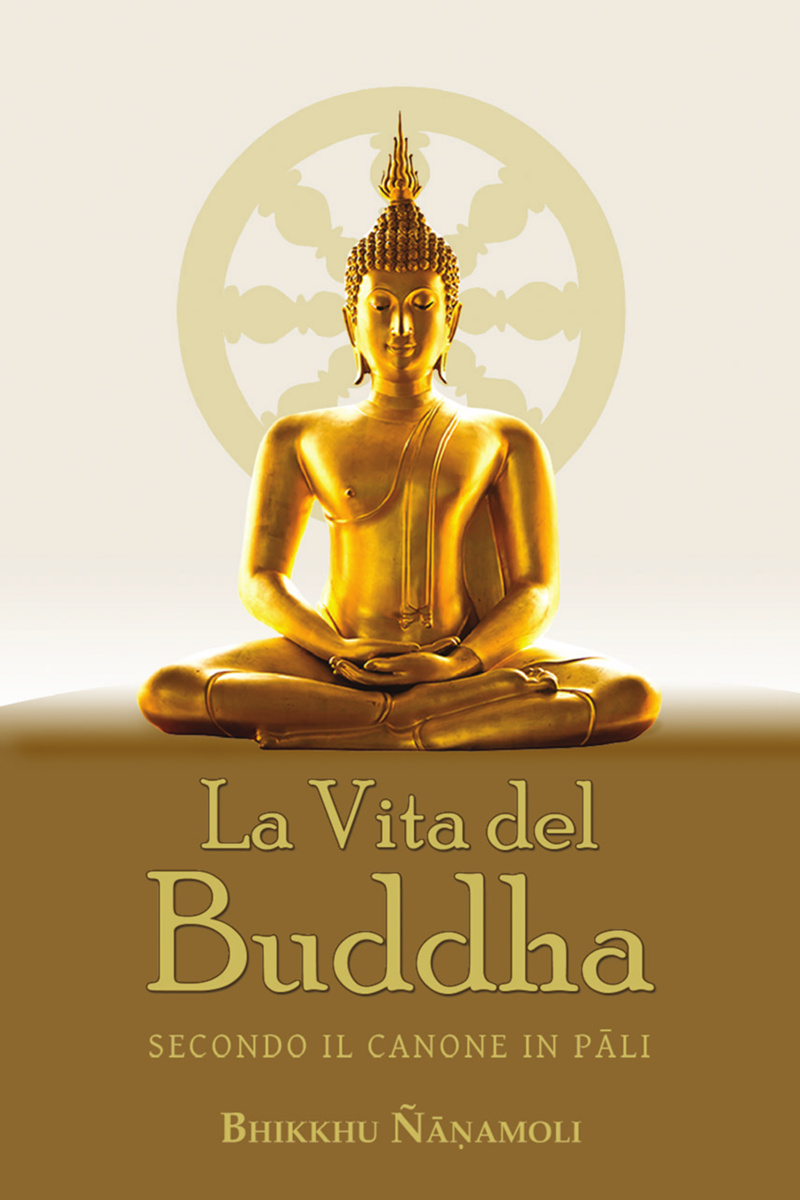
\includegraphics[height=\paperheight]{./desktop-cover.jpg}}
\fi

\cleartorecto
\thispagestyle{empty}
\vspace*{5em}

{\centering

\settowidth{\titleLength}{%
  {\Large\chapterTitleFont\scshape\MakeLowercase{\thetitle}}%
}

{\Large\chapterTitleFont\scshape\MakeLowercase{\thetitle}}\\[0.3\baselineskip]
\setlength{\xheight}{\heightof{X}}
\raisebox{0.5\xheight}{\color[gray]{0.4}\rule{\titleLength}{0.25pt}}\\[0.3\baselineskip]
{\itshape
\thesubtitle}

\vfill

\theauthor

\vspace*{5em}

}



\cleartoverso
\thispagestyle{empty}

{\copyrightsize
\centering
\setlength{\parindent}{0pt}%
\setlength{\parskip}{0.8\baselineskip}%

\thetitle\ -- \thesubtitle\\
by \theauthor

Published by \thePublisher

ISBN \theISBN

Copyright \copyright\ \thePublisher\ 2020

\vfill

{\footnotesize

This work is licensed under a Creative Commons\\
Attribution-NonCommercial-NoDerivatives 4.0 International~License.

Produced with the \LaTeX\ typesetting system, set in Gentium and Crimson Roman.

\theEditionInfo

}}


\cleartorecto
\thispagestyle{empty}

\mbox{}\vfill

{\centering

{\spectralScFont \textls{Sabbadānaṃ dhammadānaṃ jinati}}\\
``Il dono del Dhamma supera tutti i doni''

\vspace*{2\baselineskip}


\includegraphics[width=25mm]{santacittarama-logo.png}

\vspace*{4\baselineskip}

{\itshape

  Vorremmo manifestare il nostro apprezzamento,\\
  per il supporto ricevuto da molte persone\\
  nella preparazione e pubblicazione\\
  di questo libro.

  \vspace*{2\baselineskip}

  In particolare,\\
  cogliamo l’occasione per ringraziare\\
  l’Unione Buddhista Italiana (U.B.I.)\\
  che ha in gran parte finanziato la stampa\\
  mediante i fondi dell’8x1000.

}

}

\vfill\mbox{}

\clearpage
\thispagestyle{empty}

\mbox{}\vfill

{\centering

\emph{Namo tassa bhagavato arahato sammā sambuddhassa}

\vspace*{8\baselineskip}

\emph{Sabba-pāpassa akaraṇaṃ, kusalassa upasampadā,\\
sacitta-pariyodāpanaṃ; etaṃ buddhāna sāsanaṃ.}

\vspace*{2\baselineskip}

Non compiere cattive azioni, fare il bene,\\
purificare il cuore; questo è l’insegnamento dei Buddha.\\
D. 14

}

\vfill\mbox{}

\cleartorecto
\tableofcontents*

\setlength{\parindent}{18pt}
\setlength{\parskip}{0pt}

\openany

\chapter{Abbreviazioni}

{\setlength{\parindent}{0pt}\setlength{\parskip}{10pt}

\begin{tabular}{@{\hspace{15pt}} l l}
  Vin. & \emph{Vinaya Piṭaka} \\
  Sv. & \emph{Sutta-vibhanga} \\
  Pārā. & \emph{Pārājika} \\
  Saṅgh. & \emph{Saṅghādisesa} \\
  Pāc. & \emph{Pācittiya} \\
  Mv. & \emph{Mahāvagga} \\
  Cv. & \emph{Cullavagga} \\
\end{tabular}

\section{Sutta Piṭaka}

  \begin{tabular}{@{\hspace{15pt}} l l}
  D. & \emph{Dīgha-nikāya} \\
  M. & \emph{Majjhima-nikāya} \\
  S. & \emph{Saṃyutta-nikāya} \\
  A. & \emph{Anguttara-nikāya} \\
\end{tabular}

\section{Khuddaka-Nikāya}

  \begin{tabular}{@{\hspace{15pt}} l l}
  Khp. & \emph{Khuddaka-pāṭha} \\
  Ud. & \emph{Udāna} \\
  Iti. & \emph{Itivuttaka} \\
  Sn. & \emph{Sutta-nipāta} \\
  Dh. & \emph{Dhammapada} \\
  Thag. & \emph{Theragāthā} \\
\end{tabular}

I rinvii sono al capitolo (\emph{khandhaka}) e al numero della sezione per il
\emph{Mahāvagga} e per il \emph{Cullavagga}, al numero della regola per gli
altri libri del \emph{Vinaya Piṭaka,} al discorso mediante il numero o mediante
il gruppo e il numero per i libri principali del \emph{Sutta Piṭaka}, e al
numero del verso per il \emph{Dhammapada} e per le \emph{Theragāthā}.

\begin{tabular}{@{\hspace{15pt}} l l}
NDT & nota del traduttore italiano \\
\end{tabular}

}

\chapter{Prefazione dell’editore}

Questo volume è stato pubblicato dalle carte postume del defunto
venerabile bhikkhu Ñāṇamoli, la cui biografia è collocata alla fine di
questo volume. La maggior parte del libro ha ricevuto la sua forma
finale dall’autore stesso e il dattiloscritto fu preparato da lui con
accuratezza e ordine. L’introduzione era però una bozza e le appendici
menzionate nel manoscritto non furono ritrovate tra le carte
dell’autore. Più della metà del testo di questo volume era stato
pubblicato in precedenza, a puntate, in una rivista buddhista
quindicinale, \emph{Buddha Jayanti} (Colombo, 1954-1956), benché con alcuni
passi differenti. Per questa versione, verso gli ultimi suoi anni,
l’autore rivide e aumentò considerevolmente la sua traduzione dei testi
canonici e integrò la struttura dell’opera, ingegnosamente ideata,
incorporando ampio materiale dalle fonti non canoniche. Tale struttura è
spiegata nella sezione che s’intitola “Voci”.

Egli inoltre offrì nuove interpretazioni di un certo numero di parole e
termini dottrinali. In relazione a cinque di essi, l’editore ha ritenuto
opportuno tornare alle interpretazioni precedenti, apparse nella sua
traduzione pubblicata in \emph{Buddha Jayanthi} nella sua traduzione del
\emph{Visuddhimagga.} Rinvii ad alcune di queste poche alterazioni sono
contenuti nelle note dell’editore presenti a piè di pagina. Come
indicano alcune correzioni autografe presenti nel manoscritto, l’autore
ritenne che alcune di queste sue interpretazioni non potessero essere
coerentemente applicate a tutti i contesti, un fatto che ha contribuito
a far sì che l’editore abbia proceduto nel modo suddetto.

\bigskip

{\raggedleft
Nyanaponika Thera \\
Forest Hermitage \\
Kandy, Ceylon \\
Settembre 1971
\par}



\chapter{Nota alla terza edizione}

In questa terza edizione dell’ormai classica \emph{Vita del Buddha} del
venerabile Ñāṇamoli sono state corrette alcune minime incongruenze
presenti nella precedente edizione, nonché riviste alcune formulazioni
sintattiche. Per di più, vari termini dottrinali in lingua pāli che
l’autore aveva tradotto sono stati reintegrati nella stessa lingua pāli,
in quanto divenuti familiari ai lettori dei testi buddhisti ed entrati
nella terminologia corrente del Dhamma. Questi termini sono: “Buddha”,
per lo più tradotto dall’autore con “Illuminato”, una parola d’altro
canto mantenuta nel testo quando lo si è ritenuto opportuno; “Dhamma”,
da lui reso con “Legge”; “Saṅgha”, da lui indicato con “Comunità”;
“Nibbāna” spesso tradotto nell’edizione originale con “estinzione”.

Le note seguite da “Nyp.” tra parentesi tonde sono di Nyanaponika Thera,
quelle seguite da “BB” sono mie. Tutte le altre sono dell’autore.

In questa nuova edizione è presente \emph{l’Elenco delle fonti}, che
consente agli studiosi dei sutta in lingua pāli di rintracciare
facilmente i testi. Il nucleo originario di questa sezione è stato
compilato da bhikkhu Ñāṇajivako, ma è stato implementato per renderlo il
più completo possibile.

\bigskip

{\raggedleft
Bhikkhu Bodhi
\par}



\chapter{Nota alla traduzione italiana}

Per rendere più agevole la lettura, a differenza dell’edizione inglese
le note sono state collocate al fondo della pagina e non alla fine dei
capitoli. In pochissimi casi si è ritenuto opportuno aggiungere delle
note supplementari che, però, non alterano la numerazione delle note
dell’opera originale, perché anch’esse inserite al fondo della pagina ma
prive di numerazione e contrassegnate dalla sigla NDT.

Nella prima edizione la traduzione è stata
revisionata e corretta da bhikkhu Mahāpañño e poi da Danilo Briarava,
Francesca Fenu, Roberto Bertozzi e Sara Bellettato. In questa seconda edizione
l’impegno di molti ha consentito di eliminare vari refusi presenti nella prima
edizione. Con la consueta attenzione ci ha accompagnati pure Roberto Luongo,
che ha aiutato anche per la versione digitale del libro. Siamo davvero contenti
di aver avuto l’opportunità di mettere a disposizione dei lettori italiani questa
importante – anche perché fedele al Canone in pāli – biografia del Buddha.

«Ogni traduzione è una distorsione», scrisse bhikkhu Ñāṇamoli nella sua
introduzione, riferendosi ai problemi di traduzione dalla lingua pāli
all’inglese. Inevitabilmente, ciò vale anche per questo lavoro, che si è
cercato di realizzare nel modo più coscienzioso possibile. Una
traduzione letterale è stata ovviamente impossibile: sono stati perciò
necessari alcuni ritocchi che, miranti a facilitare la comprensione
del testo da parte di quanti leggeranno questa \emph{Vita del Buddha}, hanno
però inevitabilmente ritoccato anche qualche intendimento dell’autore di
questo splendido libro e, forse, pure il senso di talune parole del
Canone. Sempre per favorire la comprensione del testo, è stato
necessario inserire tra [ ] alcune parole assenti nell’edizione inglese.

\enlargethispage{\baselineskip}

In questa traduzione sono stati indicati in tondo quei termini in lingua
pāli che, come dice bhikkhu Bodhi nella \emph{Nota alla terza edizione}, sono
entrati nella terminologia corrente del Dhamma: “Buddha”, “Dhamma”,
“Saṅgha”, “Nibbāna”, “Tathāgata”. A queste si aggiungano anche
“Arahant”, “bhikkhu”, “bhikkhuṇī”, “bodhi”, “brāhmaṇa”, “deva”, “jhāna”,
“sutta”, “Vinaya” e, ovviamente, tutti i nomi di luogo (inclusi fiumi e
monti), di persona e di stirpe.

{\raggedleft
Roberto Paciocco
\par}


\chapter{La pronuncia nella lingua pāli}

Per quanto riguarda l’accento, si seguono convenzionalmente le regole
del latino: l’accento cade sulla penultima sillaba se è lunga per natura
(una vocale lunga sormontata da un trattino, oppure i dittonghi e e o,
per esempio \emph{Nibbāna, kilèsa}) o per posizione (una vocale che
precede due consonanti, per esempio \emph{avijjā}), oppure se la parola è
bisillaba; se la penultima sillaba è breve, l’accento si ritira sulla
terzultima (per esempio \emph{yàmaka}), salvo in parole di quattro o più
sillabe in cui penultima e terzultima siano brevi: in questo caso
l’accento si ritrae sulla quartultima. Nei composti, ogni parola
conserva il suo accento (per esempio \emph{Bùddha-ghòsa, Visùddhi-màgga}).
Inoltre:

\bigskip

{\setlength{\parindent}{0pt}%
\renewcommand\arraystretch{1.3}%
\fontsize{10}{14}\selectfont

\begin{tabular}{p{10mm} p{90mm}@{}}

  \emph{c} & rappresenta sempre una palatale sorda, anche davanti alle vocali \emph{a, o, u} (p. es., \emph{citta}; ma anche \emph{cakkhu}, pronunciato “ciakkhu”); \\

  \emph{g} & rappresenta sempre una gutturale sonora, anche davanti alle vocali \emph{e, i} (per esempio, \emph{garu}; ma anche \emph{gilāna}, pron. “ghìlana”); \\

  \emph{h} & è una consonante che indica un’aspirazione che deve essere pronunciata (lo \emph{hadaya}); l’aspirazione si deve far sentire anche quando segue una consonante occlusiva (p. es. in Dhamma); \\

  \emph{j} & rappresenta sempre una palatale sonora, anche davanti alle vocali \emph{a, o, u} (p. es., \emph{jana}, pron. “giana”); \\

  \emph{ṃ} & indica una nasalizzazione (p. es., \emph{saṃsāra}); \\

  \emph{ñ} & è il suono \emph{gn} dell’italiano \emph{gnosi} (p. es. in \emph{kañcuka}); \\

  \emph{ṇ} & è la nasale retroflessa (un suono intermedio fra la palatale di gnosi e la dentale di \emph{anta}) (p. es. in \emph{paṇḍu}); \\

  \emph{ṭ, h,\newline ḍ, ḍh} & sono consonanti occlusive retroflesse, pronunciate alla maniera inglese (\emph{t} di \emph{tree}) o siciliana (\emph{d} di \emph{bedda}); \\

  \emph{s} & è la sibilante sorda dell’italiano sarto (p. es. \emph{sutta}); si noti che nella lingua pāli non esiste il suono dell’italiano \emph{caso}, cioè la \emph{s} sonora o “dolce” intervocalica. \\

\end{tabular}

}

\vfill

\noindent
{\footnotesize
  (Quanto segue è ripreso, con lievi modifiche, dalla tabella posta
  all’inizio del volume \emph{Therīgāthā. Canti spirituali della monache
    buddhiste,} a cura di A.S. COMBA, Raleigh 2016.)
\par}


\chapter{Introduzione}

Quanto poco alla fine del Settecento gli europei conoscessero il Buddha
e il suo insegnamento lo sottolineò il Gibbon in una nota al XIV
capitolo del suo \emph{Decline and Fall}. Egli disse che «l’idolo
Fó»\footnote{NDT. Fó è il nome attribuito al Buddha in Cina}
è «il Fó dell’India, la cui venerazione è dominante
tra le sette dell’Hindustan, del Siam, del Tibet, della Cina e del
Giappone. Questo personaggio misterioso è, però, ancora avvolto in una
nebbia che i ricercatori della nostra Asiatic Society possono
gradualmente eliminare». Nei fatti, un gran numero di informazioni
affidabili era giunto in Europa dall’Oriente, ma esse non erano ancora
state pubblicate e restavano chiuse a chiave in forma manoscritta nelle
biblioteche. Ad esempio, il missionario gesuita Filippo Desideri portò
dal Tibet nel primo quarto del XVIII secolo un lungo e accurato
resoconto sia della vita del Buddha sia della sua dottrina: tutto ciò
rimase non pubblicato per duecento anni. Altrettanto avvenne per altri
resoconti

La “nebbia” del mistero fu dispersa dalle ricerche del XIX secolo, ma
solo per essere rimpiazzata da un pulviscolo di controversie suscitato
dalle dispute degli studiosi, nelle quali l’appena scoperta personalità
storica del Buddha parve nuovamente svanire. Non di meno, anch’esso si
disperse e, al volgere di quello stesso secolo, l’esistenza storica del
Buddha non fu più messa in dubbio, i documenti furono accertati e i
testi fissati. Tra questi documenti, il cui numero è enorme, il Canone
in lingua pāli, o \emph{Tipiṭaka}, come esso è chiamato, era considerato sia
allora sia oggi il più antico: un po’ più antico della sua controparte
in sanscrito, benché alcuni studiosi di questa lingua ancora oppongano
resistenza a tale idea. A questo proposito, lo studioso della lingua
pāli T.W. Rhys Davids appena più di un secolo dopo Gibbon poté scrivere:
«Se si pensa che Gotama Buddha lasciò dietro di sé non un certo numero
di semplici detti dai quali i suoi seguaci in seguito costruirono un
sistema o dei sistemi, ma che fu lui stesso a elaborare accuratamente la sua
dottrina ancor prima di iniziare la sua missione per quanto concerne i punti
fondamentali, e dopo la precisò solo in parte, relativamente ai dettagli. E che nel corso della
sua lunga carriera di insegnante, ebbe molto tempo per ripetere
continuamente i principi e i dettagli del sistema ai suoi discepoli e di
mettere alla prova la loro conoscenza di esso. E che, infine, i suoi
discepoli eminenti furono, come lui stesso, abituati alle più sottili
distinzioni metafisiche e addestrati in quella meravigliosa padronanza
della memoria che gli asceti dell’India di allora possedevano. Quando
questi dati di fatto vengono richiamati alla mente, si vedrà che a
ragione si può far più affidamento sugli aspetti dottrinali delle
Scritture buddhiste che non sulle altre e successive registrazioni delle
altre religioni».

La bibliografia europea sulla storia del buddhismo è ora molto ampia e,
allo stesso modo, lo è quella sulla sua letteratura e sulle sue
dottrine. L’accordo per gran parte raggiunto nell’ambito storico e
letterario, tuttavia, non si riflette su quello della dottrina. Ci sono
stati, e tuttora ci sono, numerosi e vari tentativi di dimostrare che il
buddhismo insegna il nichilismo e l’eternalismo, che è negativistico,
positivistico, ateistico, teistico, oppure che è privo di coerenza, che
è un Vedānta riformato, un umanesimo, un pessimismo, un assolutismo, un
pluralismo, un monismo, che è una filosofia, una religione, un sistema
etico, o tutto quel che vi pare opportuno. Non di meno, le parole dello
studioso russo Teodoro Stcherbatsky, scritte alla fine degli anni Venti
del XX secolo, valgono anche oggi: «Benché siano passati un centinaio
d’anni da quando gli studi scientifici sul buddhismo sono iniziati in
Europa, tuttavia brancoliamo ancora nel buio in relazione agli
insegnamenti fondamentali di questa religione e della sua filosofia.
Certo, non vi è nessun’altra religione che si sia dimostrata così
refrattaria ad essere formulata con chiarezza».

Tutti i libri che, nel Canone in lingua pāli, il \emph{Tipiṭaka}, contengono
materiale storico e discorsi sono composti in forma antologica. Il Libro
della Disciplina, il \emph{Vinaya Piṭaka}, consiste di raccolte di regole
monastiche con racconti di avvenimenti, talora molto lunghi, correlati
in un qualche modo al loro pronunciamento. I Discorsi nel \emph{Sutta Piṭaka}
sono raggruppati insieme sotto numerosi e vari titoli, ma mai
organizzati storicamente. Alla storia per scopi storici non si era a
quel tempo molto interessati in India. Perciò, una narrazione
cronologica continua della vita del Buddha deve essere messa insieme da
materiale sparso ovunque nel \emph{Vinaya Piṭaka} e nel \emph{Sutta Piṭaka}.
Questi libri contengono un quadro in sé completo e, nella sua
semplicità, fortemente contrastante con le adorne e floride versioni
successive, ad esempio con il \emph{Lalitavistarā}, che ispirò Edwin Arnold
nella sua \emph{Light of Asia}, o con la meno conosciuta introduzione alle
\emph{Storie delle Nascite} in lingua pāli nel Commentario ai \emph{Jātaka} di
Ācariya Buddhaghosa. Se confrontato con questi, il racconto offerto fino
al periodo dell’Illuminazione pare snello e lucido come una spada, come
la fiamma di una candela o una zanna d’avorio non intagliata.

Nel compilare questo racconto, è stato incluso tutto il materiale
canonico (ad eccezione del \emph{Buddhavaṃsa}) riguardante il periodo che va
dall’Ultima Nascita fino al secondo anno successivo all’Illuminazione, e
quello relativo all’ultimo anno, un materiale che praticamente
rappresenta tutta la cronologia offerta dal Canone stesso. All’evidenza
cronologica offerta dal Canone è stato dato il primo posto. La
successiva più autorevole fonte in lingua pāli, ma quanto affidabile è
difficile dirlo, è rappresentata dai \emph{Commentari} di Ācariya Buddhaghosa
(V secolo d.C), che mettono in ordine molto del materiale canonico fino
al ventesimo anno successivo all’Illuminazione, aggiungendo dettagli,
come pure la storia di Devadatta. Essi aggiungono pure un certo numero
di avvenimenti non canonici, che non sono stati qui inclusi. Infine c’è
un lavoro birmano, il \emph{Mālālaṅkāravatthu} (XV sec.?). È stato tradotto
in inglese dal vescovo Bigandet con il titolo \emph{The Story of the Burmese
Buddha} – che data qualche episodio canonico in più, ma non ha affatto,
probabilmente, autorevolezza storica ed è stato seguito solo in mancanza
di altre indicazioni. Queste sono le tre fonti utilizzate per la
sistemazione degli eventi contenuti nel \emph{Tipiṭaka}. Altri eventi
canonici di particolare interesse, benché non databili, sono stati
comunque inclusi nel capitolo “Il periodo di mezzo”. Uno o due
avvenimenti, in particolare la morte del re Bimbisāra e quella del re
Pasenadi, che sono offerti solo nei Commentari, sono stati anch’essi
aggiunti siccome la loro fonte è chiaramente indicata e perché ben si
prestano a integrare alcuni scenari. Lo scopo principale della
compilazione è quello di includere tutti gli eventi importanti fino al
ventesimo anno successivo all’Illuminazione e l’ultimo anno. I capitoli
9° e 10° sono inevitabilmente episodici. Il capitolo 11° è dedicato a
descrivere la personalità del Buddha. La “personalità”, però, è un
argomento di centrale importanza nella dottrina buddhista e, così, il
capitolo 12°, “La dottrina”, è necessariamente coinvolto in tale
argomento. In questo stesso capitolo gli elementi principali della
dottrina sono stati grosso modo messi insieme seguendo l’ordine
suggerito dai Discorsi. Non è stata tentata alcuna interpretazione: si
veda però più avanti, il paragrafo sulla “traduzione”. Il materiale è
stato invece riunito in modo tale da aiutare il lettore a fornirne una
sua propria. Un’interpretazione stereotipata corre il rischio di
scivolare in una delle metafisiche errate visioni, che il Buddha stesso
ha descritto dettagliatamente. Se il capitolo 12° è piuttosto
difficoltoso, che le ultime parole di Anāthapiṇḍika, riportate nel
capitolo 6°, siano accolte a giustificazione per la sua inclusione, e
quanti non lo trovano di loro gusto non lo leggano, in parte o del
tutto.

La lingua pāli, la cui letteratura è molto ampia, è una lingua del tutto
riservata a un solo argomento, per la precisione all’insegnamento del
Buddha. Con questo giungiamo a una differenza rispetto al buddhismo
sanscrito o alla chiesa latina: si tratta di un fatto che gli conferisce
una particolare nettezza, senza riscontri in Europa. È una delle lingue
del gruppo indo-europeo ed è imparentata con il sanscrito, ma ha un
differente sapore. Lo stile dei sutta (Discorsi) è connotato da una
produttiva semplicità, che si accoppia a una ricchezza idiomatica che lo
rende un veicolo particolarmente raffinato al quale è difficile rendere
giustizia con una traduzione. Questo è il problema principale. Ce n’è
però un altro. La speciale caratteristica delle ripetizioni parola per
parola di passi, frasi e proposizioni che si presentano in
continuazione. Questa peculiarità è con ogni probabilità originariamente
dovuta al fatto che questi “libri” furono pensati per la recitazione. In
Europa siamo abituati a ripetizioni formali nella musica sinfonica
durante i concerti e magari alle ripetizioni in poesia, ma le troviamo
strane nella prosa. Al lettore non abituato a tali ripetizioni, nella
misura in cui esse compaiono nella lingua pāli, paiono sgradevoli su una
pagina a stampa. Perciò, esse sono state per la maggior parte eliminate
nella traduzione mediante vari stratagemmi, tuttavia sempre prestando
particolare attenzione alla conservazione dell’originaria architettura
della forma dei discorsi, che è una delle più rimarchevoli
caratteristiche espressive del Buddha. Nello stesso tempo, però, alcune
ripetizioni sono state conservate, in quanto valorizzano la preziosa
tecnica del “repetita iuvant”. Queste ripetizioni, se riscontrabili
parola per parola in lingua pāli, sono tradotte parola per parola anche
in inglese. Non è stato facile conciliare i due principali obiettivi di
questa traduzione, fedeltà letterale e corrispondenza idiomatica. Ogni
traduzione è una distorsione. Una gran cura è stata tuttavia riposta
nella coerente restituzione di termini tecnici – evitando “variazioni
eleganti” – e tali termini in lingua pāli potranno essere rinvenuti
nell’Indice, a fianco degli equivalenti in lingua
inglese.\footnote{NDT. Nell’Indice di questo volume, tali termini in lingua pāli è possibile rinvenirli tra (), a fianco delle parole italiane.}
La scelta dei termini equivalenti in inglese
è stata effettuata con grande attenzione e assistita dall’intento di
consentire una coerente analisi delle forme inglesi per uno studio di
genere ontologico e della teoria percettiva e cognitiva insita – non a
caso, sembrerebbe – nei Discorsi.

Vi sono casi in cui la spiegazione dei Commentari in relazione al
significato delle parole è in conflitto con quella offerta dal
\emph{Dictionary} della Pāli Text Society. In tali casi la preferenza è stata
data ai Commentari. Dei casi più importanti si rende conto nelle
note.\footnote{NDT. Segue un paragrafo, qui omesso, relativo alla pronuncia delle parole in lingua pāli per gli anglofoni. In relazione alla pronuncia di tali parole per gli italiani, si veda la \emph{Nota del traduttore}.}

Infine, qualche parola sulla forma di questa compilazione. La forma in
cui si presenta, non pensata per una divulgazione di massa, è stata
suggerita dal materiale che, come è stato detto, fu all’origine recitato
oralmente. Il Vinaya Piṭaka stesso suggerisce le “Voci” (si veda il cap.
16 e l’elenco delle voci precedenti il cap. 1) che “recitarono” il
Canone durante i Concili. I due “Narratori” sono, per così dire, due
compagni di uguale rango. In contrasto con quello che le “Voci” hanno da
dire, le parti spettanti ai “Narratori” sono per scelta caratterizzate
sia da uno stile piatto sia dalla massima brevità.

\bigskip

{\raggedleft
Bhikkhu Ñāṇamoli
\par}



\setlength{\parindent}{0pt}
\setlength{\parskip}{8pt}

\chapter{Mappa dell'India centro-orientale}

\vspace*{\baselineskip}

{\centering
  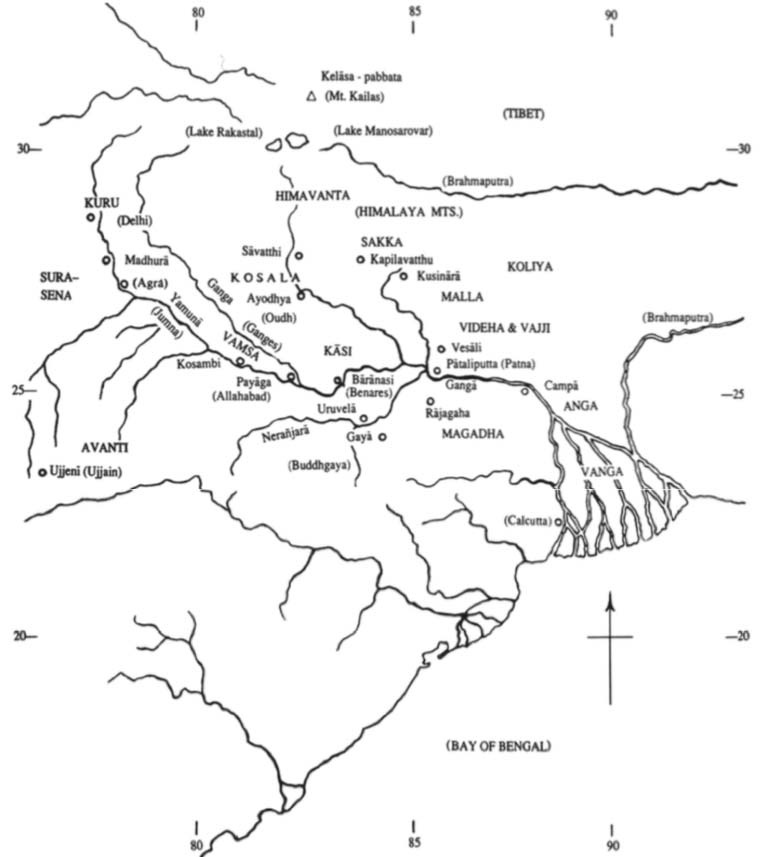
\includegraphics[width=\linewidth]{mappa.jpg}
\par}

\vspace*{1.5\baselineskip}

La mappa — tratta dalla \emph{Cambridge History of India, I: Ancient India}, ed.
by E.J. R Apson, Cambridge 1922, Map. 5 — mostra alcuni dei principali nomi
di luogo menzionati nel Canone in lingua pāli. I nomi moderni sono
racchiusi tra parentesi tonde.


\chapter{Voci}

\narrator{Primo narratore.} È un commentatore del nostro tempo che offre cognizioni
introduttive, un osservatore imparziale con una generale conoscenza
degli eventi.

\narrator{Secondo narratore.} È un commentatore che propone informazioni storiche e
culturali presenti solo nei Commentari in lingua pāli, soprattutto in
quelli di Buddhaghosa, che risalgono al V secolo d.C. Ha la funzione di
offrire il materiale strettamente indispensabile per una
contestualizzazione storica e, occasionalmente, sintetizza parti del
Canone stesso.

\voice{Prima voce.} È la voce di Ānanda, discepolo e assistente personale del
Buddha, che recitò i Discorsi (o sutta) durante il Primo Concilio,
tenutosi a Rājagaha tre mesi dopo la morte e il \emph{Parinibbāna} del
Buddha.

\voice{Seconda voce.} È la voce di Upāli, discepolo del Buddha, che durante il
Primo Concilio recitò la Disciplina (o Vinaya).

\voice{Terza voce.} È un partecipante al Secondo Concilio, tenutosi cento anni
dopo il \emph{Parinibbāna} del Buddha, che nel XVI capitolo narra gli eventi
verificatisi prima e dopo il Primo Concilio.

\cantor{Cantore}

\begin{quote}
Questa voce recita alcuni versi \\
in forma di brevi poemi o inni \\
che nel Canone in lingua pāli \\
non sono introdotti \\
dalle tradizionali parole \\
pronunciate da Ānanda, «Così ho udito», \\
né sono presenti nella Disciplina.
\end{quote}



\openright

% Page 1 is the first page of the first chapter.
\mainmatter

\chapter{La nascita e i primi anni}

\narrator{Primo narratore.} La storia dell’India inizia con la vita del Buddha
Gotama. Più esattamente, è a questo punto che la memoria storica rimpiazza
l’archeologia e la leggenda. Le notizie fornite dalla vita e dagli insegnamenti
del Buddha – sono i primi testi a essere ritenuti storicamente attendibili –
indicano l’esistenza di una civiltà stabile e assai sviluppata che richiese
molto tempo per giungere a maturazione. Il Buddha ottenne l’Illuminazione nei
pressi di Uruvelā, nella pianura del Gange, chiamata la “Terra di Mezzo”. In
base al modo in cui sono misurate le distanze in India, non si trattava di
luoghi molto distanti dall’antichissima e santa città di Benares. Egli aveva
trentacinque anni, e per sei anni s’era sforzato per ottenere l’Illuminazione.
D’allora in poi, per quarantacinque anni, errò fra vari luoghi dell’India
centrale, spiegando in continuazione le Quattro Nobili Verità da lui scoperte.
Così come calcolato in Europa, il \emph{Parinibbāna} finale ebbe luogo nel 483
a.C., secondo la tradizione nel giorno di luna piena del mese di maggio. Il
periodo nel quale egli visse sembra essere stato eccezionalmente calmo, la
società era stabile e i governi ben organizzati, in forte contrasto rispetto a
quanto avvenne prima e dopo.

\narrator{Secondo narratore.} Tre mesi dopo il \emph{Parinibbāna} del Buddha, i
suoi discepoli più longevi sopravvissutigli convocarono un concilio di
cinquecento monaci anziani per mettersi d’accordo sulla forma in cui
l’insegnamento del Maestro doveva essere tramandato alla posterità. Tra questi
cinquecento monaci, che avevano tutti realizzato l’Illuminazione, Upāli fu
l’autorità riconosciuta per le regole di condotta e le circostanze che avevano
indotto a stilarle. La parte principale del “Canestro della Disciplina” – il
\emph{Vinaya Piṭaka} – fu composto durante il concilio, sulla base della sua
recitazione.

Quando ebbe finito, Ānanda fu invitato a recitare i Discorsi. Ānanda, che era
stato l’assistente personale del Buddha durante gli ultimi suoi ventiquattro
anni, era dotato di una memoria straordinaria. Quasi tutta la raccolta dei
Discorsi, con le rispettive ambientazioni, contenuti nel “Canestro dei Discorsi”
(il \emph{Sutta Piṭaka}) fu composto sulla base della sua recitazione. Upāli
iniziò ogni resoconto con le parole \emph{tena samayena} – «Avvenne questo» –
mentre Ānanda cominciò ogni discorso riferendo il luogo in cui il Buddha parlò e
la persona alla quale egli si rivolse, iniziando con le parole \emph{evaṃ me
  sutaṃ} – «Così ho udito».

\narrator{Primo narratore.} Questa narrazione della vita del Buddha è tratta da
tali due “Canestri”. Come siano riusciti a giungere fino a noi, lo diremo in
seguito. Qui, per cominciare, offriamo il racconto dell’ultima nascita del
Buddha, descritta da lui stesso e in seguito riferita da Ānanda durante il
concilio. Le parole furono pronunciate nella lingua del Buddha, nota come lingua
pāli.

\voice{Prima voce.} Così ho udito. Una volta il Beato\footnote{Una traduzione
  letterale dell’aggettivo \emph{bhagavant} è impossibile. Viene perciò reso con
  “Beato”. Buddhaghosa nel suo \emph{Visuddhimagga} (VII, pp. 53 ss.) offre
  numerose spiegazioni in merito.} soggiornava a Sāvatthī, nel Boschetto di
Jeta, nel parco di Anāthapiṇḍika. Un certo numero di bhikkhu\footnote{La parola
  “bhikkhu” (in sanscrito: \emph{bhikṣhu}) è stata lasciata in lingua pāli.
  Etimologicamente deriva da \emph{bhikkhā} (elemosina). Vi sono però altre
  derivazioni “semantiche” più antiche: \emph{saṃsāre bhayaṃ ikkhatī ti bhikkhu}
  («colui che vede la paura nel ciclo delle rinascite, e perciò è un “veggente
  della paura”»). Un bhikkhu è un membro a pieno titolo della comunità monastica
  (Saṅgha), ma il fatto che vi sia pienamente accolto non comporta alcun voto
  irrevocabile.} era in attesa nella sala delle riunioni, dove si erano raccolti
al ritorno dalla questua, dopo il termine del pasto. Frattanto, dicevano tra
loro: «È meraviglioso, amici, è stupefacente come il potere e l’energia del
Perfetto gli consentano di avere conoscenza dei Buddha del passato che
realizzarono la completa estinzione delle contaminazioni, che sbrogliarono la
matassa, che spezzarono il cerchio, che posero fine al girare in tondo e che
andarono al di là di ogni sofferenza, e così di sapere: queste furono le nascite
di quei Beati, questi i loro nomi, questa la loro stirpe, questa la loro virtù,
questa la loro concentrazione, questa la loro comprensione, questo il loro
dimorare, questo il modo della loro liberazione».

Dopo che queste parole furono pronunciate, il venerabile Ānanda disse ai
bhikkhu: «Gli Esseri Perfetti sono meravigliosi, amici, e hanno meravigliose
qualità. Gli Esseri Perfetti sono stupefacenti e hanno stupefacenti qualità».

Il loro discorso non era ancora terminato quando già era sera, e il Beato, che
aveva interrotto il suo ritiro, raggiunse la sala delle riunioni e si mise a
sedere nel posto preparatogli. Chiese allora ai bhikkhu: «Per parlare di quale
argomento vi siete qui riuniti? Quale discorso è stato lasciato incompiuto?».

Gli fu allora riferito quello che i bhikkhu e il venerabile Ānanda avevano
detto, e loro soggiunsero: «Signore, questo è il discorso lasciato incompiuto
perché è arrivato il Beato». Il Beato allora si rivolse al venerabile Ānanda:
«Se è così, Ānanda, spiega più a fondo le meravigliose e stupefacenti qualità
degli Esseri Perfetti».

«Ho sentito e imparato questo, Signore, dalle labbra stesse del Beato.
Consapevole e con piena presenza mentale il Bodhisatta, l’Essere Dedito
all’Illuminazione, apparve nel paradiso dei Gioiosi.\footnote{Il paradiso dei
  Gioiosi (\emph{Tusita}). La cosmologia di quei tempi descrive molti paradisi:
  in particolare sei paradisi nei quali sono goduti tutti i piaceri sensoriali;
  al di sopra di questi, dodici paradisi di Brahmā – il “Mondo della Suprema
  Divinità” – nei quali la consapevolezza è del tutto purificata dalla brama,
  benché non lo sia da una sua futura potenzialità. Secondo il Commentario, in
  questi ultimi paradisi la forma materiale è rarefatta dall’assenza dei tre
  sensi dell’odorato, del gusto e del tatto, nonché del sesso; tali paradisi
  corrispondono agli stati raggiungibili dagli esseri umani nei primi quattro
  jhāna (stati di assorbimento meditativo). Oltre a questi, per meglio dire,
  affinamenti dei quattro jhāna, vi sono quattro stati infiniti “privi di
  forma”, nei quali ogni percezione della forma materiale e delle differenze è
  trascesa: corrispondono all’infinità dello spazio e della coscienza, al
  nulla-è, alla né-percezione-né-non-percezione. La rinascita in ognuno di essi
  è impermanente e seguìta da nuove rinascite fino a quando non si ottiene il
  Nibbāna, il non-creato.} Ed è questo che io ricordo come meravigliosa e
stupefacente qualità del Beato».

«Ho sentito e imparato questo, Signore, dalle labbra stesse del Beato.
Consapevole e con piena presenza mentale il Bodhisatta restò nel paradiso dei
Gioiosi».

«Per l’intera durata di quella vita il Bodhisatta restò nel paradiso dei
Gioiosi».

«Consapevole e con piena presenza mentale scomparve dal paradiso dei Gioiosi e
discese nel grembo di sua madre».

«Quando il Bodhisatta scomparve dal paradiso dei Gioiosi ed entrò nel grembo di
sua madre, una luce grande e incommensurabile che superava per splendore quella
degli dèi apparve nel mondo con i suoi deva, con i suoi Māra e con le sue
divinità, in questa generazione con i suoi monaci e brāhmaṇa, con i suoi
principi e uomini.\footnote{Seguendo il Commentario, \emph{sadevamanussānaṃ} è
  stato tradotto con «con i suoi principi e uomini». È il senso complessivo a
  richiederlo, mentre “deva” era anche la forma normale per rivolgersi a un re.}
E anche nelle intercapedini di quell’abissale mondo fatto di vuoto, tenebre e
assoluta oscurità, dove la luna e il sole, potenti e possenti come sono, non
riescono a far prevalere la loro luce – pure là comparve una luce grande e
incommensurabile che superava per splendore quella degli dèi, e le creature nate
in queste intercapedini grazie a quella luce riuscirono a percepirsi
vicendevolmente: “Così, sembra che altre creature siano apparse qui!”. E questo
sistema di diecimila mondi si scosse, tremò e vacillò, e anche lì comparve una
luce grande e incommensurabile che superava per splendore quella degli dèi».

«Quando il Bodhisatta discese nel grembo di sua madre, quattro divinità giunsero
a proteggerlo dai quattro angoli del mondo, così che nessun essere umano,
non-umano né alcun altro potesse in alcun modo nuocere a lui o a sua madre».

«Quando il Bodhisatta discese nel grembo di sua madre, lei divenne
intrinsecamente pura, si astenne dall’uccidere esseri viventi, dal prendere quel
che non è dato, dal comportamento non casto, dalla falsa parola, e
dall’indulgere al vino, ai liquori e alle bevande fermentate».

«Quando il Bodhisatta discese nel grembo di sua madre, lei non fu più toccata
dai cinque aspetti del desiderio sensoriale, e divenne inaccessibile per gli
uomini di mente lussuriosa».

«Quando il Bodhisatta discese nel grembo di sua madre, lei nel contempo
possedeva i cinque aspetti del desiderio sensoriale, ed essendone dotata e
corredata, ne era gratificata».

«Quando il Bodhisatta discese nel grembo di sua madre, in lei non sorse alcun
genere di afflizione: era beata e priva di ogni affaticamento corporale».

«Come se un filo blu, giallo, rosso, bianco o marrone fosse introdotto in una
pregiata gemma di berillo ben tagliata a otto facce, trasparente come acqua
purissima, e un uomo con gli occhi sani la prendesse in mano esaminandola in
questo modo – “Questa è una pregiata gemma di berillo ben tagliata a otto facce,
trasparente come acqua purissima, e un filo blu, giallo, rosso, bianco o marrone
è introdotto in essa” – così anche la madre del Bodhisatta lo vedeva nel proprio
grembo con tutte le sue membra, dotato di ogni facoltà».

«Sette giorni dopo la nascita del Bodhisatta, sua madre morì e rinacque nel
paradiso dei Gioiosi».

«Altre donne partoriscono dopo aver tenuto in grembo il bambino per nove o dieci
mesi, ma non la madre del Bodhisatta. Lei partorì dopo averlo tenuto in grembo
per dieci mesi esatti».

«Altre donne partoriscono sedute o distese, ma non la madre del Bodhisatta. Lei
lo partorì stando in piedi».

«Quando il Bodhisatta uscì dal grembo della madre, egli non toccò la terra. Le
quattro divinità lo accolsero e lo posero di fronte alla madre, dicendo:
“Gioisci, o regina, hai dato alla luce un figlio con un grande potere”».

«Quando il Bodhisatta uscì dal grembo della madre, fu come se una gemma fosse
messa in un panno di Benares. La gemma non macchierebbe il panno né il panno
macchierebbe la gemma – perché no? – perché entrambi sono puri. Così anche il
Bodhisatta uscì dal grembo della madre immacolato, senza essere macchiato da
acqua, umori, sangue o qualsiasi altro genere d’impurità, uscì pulito e
immacolato.

«Quando il Bodhisatta uscì dal grembo della madre, due getti d’acqua si
riversarono dal cielo, uno fresco e uno caldo, per lavare il Bodhisatta e sua
madre».

«Appena il Bodhisatta nacque, rimase saldamente in piedi sul terreno, poi fece
sette passi a nord e, mentre un bianco parasole era tenuto sul suo capo,
sorvegliò ogni angolo del mondo. Proferì le parole del Signore del Branco: “Nel
mondo sono il Supremo, nel mondo sono il Migliore, nel mondo sono l’Eminente.
Questa è l’ultima nascita, ora non ci saranno più rinascite in vite future”».

«Quando il Bodhisatta uscì dal grembo della madre, una luce grande e
incommensurabile, che superava per splendore quella degli dèi, apparve nel mondo
con i suoi deva, con i suoi Māra e con le sue divinità, in questa generazione
con i suoi monaci e brāhmaṇa, con i suoi principi e uomini. E anche nelle
intercapedini di quell’abissale mondo fatto di vuoto, tenebre e assoluta
oscurità, dove la luna e il sole, potenti e possenti come sono, non riescono a
far prevalere la loro luce – pure là comparve una luce grande e incommensurabile
che superava per splendore quella degli dèi, e le creature nate in queste
intercapedini grazie a quella luce riuscirono a percepirsi vicendevolmente:
“Così, sembra che altre creature siano apparse qui!”. E questo sistema di
diecimila mondi si scosse, tremò e vacillò, e anche lì comparve una luce grande
e incommensurabile che superava per splendore quella degli dèi».

«Tutte queste cose ho udito e imparato dalle labbra stesse del Beato. E io le
ricordo come meravigliose e stupefacenti qualità del Beato».

«Se è così, Ānanda, ricorda anche questa come meravigliosa e stupefacente
qualità di un Essere Perfetto: le sensazioni piacevoli, dolorose o neutre di un
Essere Perfetto sono da lui conosciute quando sorgono, sono da lui conosciute
quando sono presenti, e sono da lui conosciute quando si placano; le sue
percezioni sono da lui conosciute quando sorgono, sono da lui conosciute quando
sono presenti, sono da lui conosciute quando si placano; i suoi pensieri sono da
lui conosciuti quando sorgono, sono da lui conosciuti quando sono presenti, sono
da lui conosciuti quando si placano».

«E anche questo ricordo, o Signore, come meravigliosa e stupefacente qualità del
Beato».

Questo è ciò che il venerabile Ānanda disse. Il Maestro approvò. I bhikkhu
furono soddisfatti, e si deliziarono delle parole del venerabile Ānanda.

\suttaRef{M. 123; cf. D. 14}

\narrator{Primo narratore.} Come un veggente brāhmaṇa – un veggente del “divino”
o della casta dei sacerdoti – predisse la futura Illuminazione è raccontato in
un canto.

\begin{quote}
\cantor{Cantore}

Il Saggio Asita, nella sua meditazione diurna, \\
vide che gli dèi, quelli della Compagnia dei Trenta, \\
erano felici e gioiosi e, vestiti di splendore, sventolavano bandiere, \\
rumorosamente si rallegravano assieme al loro sovrano Sakka. \\
Quando vide gli dèi così felici ed esultanti, \\
rispettosamente li salutò e rivolse loro questa domanda:

«Perché la Compagnia degli dèi è così gioiosa? \\
Perché sventolano bandiere in questo modo? \\
Mai ci fu una celebrazione del genere, \\
nemmeno dopo la battaglia con i dèmoni, \\
quando gli dèi vinsero e i dèmoni furono sconfitti. \\
Qual è la meraviglia che hanno udito e che tanto li delizia? \\
Guardate come cantano, gridano e strimpellano chitarre, \\
come applaudono e danzano ovunque. \\
O voi, che dimorate sugli ariosi picchi del Monte Meru, \\
vi prego, non lasciatemi nel dubbio, buoni signori».

«In una città dei Sakya, nella terra di Lumbinī \\
è nato nel mondo degli uomini \\
un Essere che otterrà l’Illuminazione, un Gioiello Inestimabile \\
che porterà loro benessere e floridezza. \\
Per questo siamo gioiosi in modo così stravagante. \\
L’Essere Unico, la Personalità Sublime, \\
il Signore di tutti gli Uomini e l’Eminente del genere umano \\
farà girare la Ruota nel Boschetto degli Antichi Veggenti \\
con il ruggito del leone, il sovrano di tutti gli animali».

Quando udì queste parole, il Saggio si affrettò, \\
andò nella dimora di Suddhodana. \\
Lì sedette: «Dov’è il bimbo?». \\
Ai Sakya chiese: «Mostratemelo» \\
Quando i Sakya mostrarono il bimbo ad Asita \\
il suo colore era puro \\
come i raggi d’oro brillante lavorato in un crogiolo, \\
splendente e chiaro.

La gioia del rapimento estatico inondò il cuore di Asita \\
nel vedere il bimbo luminoso come una fiamma e puro \\
come il Signore delle Stelle che cavalca nel cielo, \\
abbagliante come il sole in un autunno senza nubi \\
mentre nella volta celeste gli dèi tenevano sul suo capo \\
un parasole nervato da migliaia di cerchi, \\
brandendo dorati piumini scaccia-insetti, \\
senza che nessuno vedesse \\
chi reggeva il parasole e i piumini.

Il saggio dai capelli intrecciati, chiamato
Kaṇhasiri,\footnote{\emph{Kaṇhasiri} significa “Buio Splendore” (l’equivalente in sanscrito di \emph{Kaṇha} è \emph{Kṛṣṇa}).} \\
vedendo il bimbo come un gioiello d’oro su broccato, \\
con il bianco parasole tenuto sul suo capo, \\
lo accolse colmo di gioia e di felicità. \\
Appena ricevette il Signore dei Sakya, \\
l’esperto interprete di marchi e segni \\
esclamò con cuore pronto e fiducioso: \\
«Tra la razza dei bipedi egli è unico». \\
Ricordò e vedendo il suo stesso destino \\
per la grande tristezza le lacrime gli velarono gli occhi. \\
I Sakya lo videro piangere, e gli chiesero: \\
«Qualche sventura accadrà al nostro principe?». \\
Ai Sakya ansiosi egli rispose: \\
«Prevedo che nessun pericolo toccherà il bimbo, \\
tanto meno qualche rischio l’attende. \\
Siate certi che non è uomo di secondo rango, \\
perché egli raggiungerà la sommità della vera conoscenza. \\
Un profeta d’impareggiabile purezza, \\
grazie alla compassione per la moltitudine metterà \\
in moto la Ruota del Dhamma e diffonderà la sua santa vita. \\
A me resta poco però da vivere, \\
nel frattempo morirò. Non potrò ascoltare \\
l’incomparabile Eroe insegnare il Buon Dhamma. \\
È questo a intristirmi, è questa la perdita che m’addolora».

Colui che visse la santa vita lasciò la stanza centrale del palazzo \\
dopo aver colmato i Sakya di sovrabbondante gioia. \\
Andò dal figlio di sua sorella e, mosso da compassione, \\
gli disse del futuro dell’impareggiabile Eroe che trova il Dhamma.

«Quando sarai raggiunto dalla notizia che egli è illuminato, \\
e sta vivendo il Dhamma da lui stesso scoperto, \\
va da lui, chiedigli il suo insegnamento \\
e vivi con il Beato la santa vita».

Così Nālaka, che aveva accumulato grandi meriti, \\
avvisato da chi il suo bene voleva, da chi aveva predetto \\
la venuta dell’Essere Perfetto, conseguì la massima purezza, \\
attese con i sensi raffrenati, aspettando il Vittorioso.

Sentendo che il Nobile Vittorioso \\
aveva fatto girare la Ruota, andò da lui. \\
Vide il Signore di tutti i Veggenti, \\
e credette in lui quando lo vide. \\
Adempiendo il volere di Asita, \\
egli chiese al Perfetto Saggio \\
del Silenzio Supremo.
\end{quote}

\suttaRef{Sn. 3:11}

\narrator{Primo narratore.} Benché la letteratura successiva offra molti
dettagli sui primi anni, il \emph{Tipiṭaka} dice pochissimo in proposito. Fa
riferimento a due soli episodi. Innanzitutto, il ricordo della meditazione sotto
l’albero di melarosa mentre il padre del Bodhisatta era al lavoro. Stava
svolgendo l’aratura cerimoniale per l’apertura della stagione della semina, dice
il Commentario. È un ricordo sul quale ci soffermeremo in seguito. Poi il
racconto delle “tre riflessioni”, che corrispondono a tre dei “messaggeri” –
l’anziano, il malato e il defunto – visti dal precedente Buddha Vipassī.

\suttaRef{D. 14}

\voice{Prima voce.} «Ero delicato, molto delicato, massimamente
delicato.\footnote{Queste circostanze sono altrove considerate essere costanti
  per tutti i Bodhisatta nella loro ultima esistenza (D. 14). Nel
  \emph{Tipiṭaka} la narrazione dei “quattro messaggeri” – l’anziano, il malato,
  il cadavere e il monaco – è riferita solo al precedente Buddha Vipassī, non al
  Buddha Gotama. Racconti successivi la collegano anche al Buddha Gotama.}
Laghetti adorni di fiori erano allestiti nella casa di mio padre per mio solo
beneficio. In uno fiorivano gigli blu, in un altro gigli bianchi, in un altro
ancora gigli rossi. Non usavo legno di sandalo a meno che non provenisse da
Benares. Il mio turbante, la mia tunica, gli indumenti della parte più bassa del
corpo e il mantello erano fatti di stoffa di Benares. Un bianco parasole era
tenuto sul mio capo di giorno e di notte, così che né il freddo né il caldo, né
la polvere né la sabbia e neanche la rugiada potessero infastidirmi».

«Avevo tre palazzi. Uno per la stagione fredda, uno per la stagione calda e un
altro per quella delle piogge. Nel palazzo per le piogge ero intrattenuto da
menestrelli, tra i quali non c’erano uomini. Durante i quattro mesi delle piogge
non scendevo mai nella parte inferiore del palazzo. Benché in altre case i pasti
per i domestici e gli inservienti prevedevano riso spezzato e zuppa di
lenticchie, nella casa di mio padre a loro era dato riso bianco e carne».

«Mentre godevo di tale autorità e buona sorte, tuttavia pensavo: “Quando un uomo
ignorante e ordinario, che è soggetto all’invecchiamento, non è al sicuro
dall’invecchiamento, vede un altro che è anziano, si sente scosso, umiliato e
disgustato perché dimentica che lui stesso non fa eccezione. Anch’io sono
soggetto all’invecchiamento, non sono al sicuro dall’invecchiamento, e perciò
non mi si addice essere scosso, umiliato e disgustato vedendo un altro che è
anziano”. Quando facevo questa riflessione, la vanità della giovinezza mi
abbandonava del tutto».

«Pensavo: “Quando un uomo ignorante e ordinario, che è soggetto alle malattie,
non è al sicuro dalle malattie, vede un altro che è malato, si sente scosso,
umiliato e disgustato perché dimentica che lui stesso non fa eccezione. Anch’io
sono soggetto alle malattie, non sono al sicuro dalle malattie, e perciò non mi
si addice essere scosso, umiliato e disgustato vedendo un altro che è malato”.
Quando facevo questa riflessione, la vanità della salute mi abbandonava del
tutto».

«Pensavo: “Quando un uomo ignorante e ordinario, che è soggetto alla morte, non
è al sicuro dalla morte, vede un altro che è morto, si sente scosso, umiliato e
disgustato perché dimentica che lui stesso non fa eccezione. Anch’io sono
soggetto alla morte, non sono al sicuro dalla morte, e perciò non mi si addice
essere scosso, umiliato e disgustato vedendo un altro che è morto”. Quando
facevo questa riflessione, la vanità della vita mi abbandonava del tutto».

\suttaRef{A. 3:38}


\chapter{Lo sforzo per l'Illuminazione}

\narrator{Primo narratore.} Il racconto della Rinuncia offerto nei Piṭaka è,
nella sua nuda semplicità, suggestivo. In questa più antica versione, gli
elaborati dettagli di quelle successive sono assenti, come lo sono quelli della
nascita e dei primi anni. Ecco il racconto tratto da vari discorsi pronunciati
per diverse persone.

\voice{Prima voce.} «Prima della mia Illuminazione, quando ero ancora solo un
Bodhisatta non illuminato, essendo io stesso ancora soggetto a nascita,
vecchiaia, malattia, morte, dolore e contaminazioni, cercavo quel che era pure
soggetto a queste cose. Allora pensai: “Perché, essendo io stesso soggetto a
nascita, vecchiaia, malattia, morte, dolore e contaminazioni, cerco quel che è
pure soggetto a queste cose? E se, essendo io stesso soggetto a queste cose e
vedendo in esse il pericolo, cercassi invece la suprema e incontaminata
cessazione della schiavitù, il Nibbāna, privo di nascita, privo di vecchiaia,
privo di malattia, privo di morte e privo di dolore?”».

\suttaRef{M. 26}

«Prima della mia Illuminazione, quando ero ancora solo un Bodhisatta non
illuminato, pensai: “La vita in famiglia è affollata e polverosa, l’abbandono di
essa comporta spaziose aperture. Vivendo in famiglia non è facile condurre una
santa vita assolutamente perfetta e immacolata come una conchiglia ben lucidata.
E se mi rasassi i capelli e la barba, indossassi l’abito ocra, e rinunciassi
alla vita in famiglia per una senza dimora?”».

\suttaRef{M. 36, 100}

«In seguito, quando ero ancora giovane, un ragazzo dai capelli neri benedetto
dalla giovinezza, mi rasai i capelli e la barba e – benché mia madre e mio padre
desiderassero altro per me e si addolorassero con il volto pieno di lacrime –
indossai l’abito ocra e rinunciai alla vita in famiglia per una senza dimora».

\suttaRef{M. 26, 36, 85, 100}

\cantor{Cantore}

\begin{quote}
Ora racconterò la rinuncia alla vita in famiglia, \\
come egli, il possente Veggente, lasciò la sua casa, \\
cosa gli fu chiesto e come descrisse \\
la ragione della sua rinuncia. \\
La vita affollata vissuta in una casa \\
esala un’atmosfera polverosa, \\
ma il suo abbandono comporta spaziose aperture: \\
questo egli vide, e scelse l’abbandono della vita in famiglia. \\
Nel farlo rifiutò \\
ogni cattiva azione del corpo, \\
respinse ogni genere di errata parola \\
e rese inoltre retti i suoi mezzi di sostentamento. \\
Andò nella città di Rājagaha, \\
nel castello di Magadha, \\
là, egli – il Buddha – fece la questua, \\
con più di un marchio d’eccellenza. \\
Il re Bimbisāra \\
lo vide passare dal suo palazzo, \\
e quando egli vide l’eccellenza \\
di tutti i suoi marchi, egli disse: \\
«Guardate, signori, quanto è bello quell’uomo, \\
quanto è maestoso, quanto pura e perfetta è la sua condotta, \\
con gli occhi bassi e consapevole, guarda \\
alla sola distanza d’un giogo d’aratro davanti a lui, \\
non è di basso lignaggio. \\
Mandate subito dei messi reali \\
che seguano la strada percorsa dal bhikkhu». \\
I messi vennero subito inviati \\
e seguirono la sua scia dappresso: \\
«Che strada prenderà il bhikkhu? \\
Qual è il luogo che ha scelto per dimora? \\
Vaga di casa in casa, \\
custodendo le porte dei sensi con vero contenimento, \\
pienamente consapevole e cosciente. \\
Ha subito colmato la sua ciotola per l’elemosina, \\
ora ha terminato la sua questua. \\
Il Saggio s’incammina e lascia la città, \\
prendendo la via per Paṇḍava: \\
deve vivere sull’altura di Paṇḍava».

Quando egli raggiunse la sua dimora \\
i messi lo raggiunsero, \\
ma uno di loro tornò indietro \\
per portare al re la risposta alla sua domanda:

«Il bhikkhu, sire, come una tigre, \\
come un toro o come un leone, \\
abita nella caverna di un monte \\
sul versante orientale di Paṇḍava».

Il guerriero ascoltò il racconto del messaggero, \\
prendendo poi una carrozza reale \\
in fretta uscì dalla città \\
verso l’altura di Paṇḍava. \\
Con il carro andò più lontano che poté, \\
e poi ne discese, \\
percorse a piedi la breve distanza che restava \\
finché arrivò vicino al Saggio.

Il re sedette, scambiò saluti, \\
e gli chiese delle sue condizioni fisiche. \\
Quando questo scambio di cortesie \\
fu terminato, il re gli disse queste parole: \\
«Sei piuttosto giovane, un ragazzo, \\
un uomo nella prima fase della vita. \\
Hai il bell’aspetto d’un uomo \\
d’alto e nobile lignaggio guerriero, \\
uno adatto ad adornare un esercito di prim’ordine \\
per guidare le truppe di elefanti. \\
Ti offro una fortuna: afferrala. \\
Quali i tuoi natali? Dimmelo».

«C’è una terra prosperosa, sire, \\
e forte, proprio di fronte alle pendici dell’Himalaya, \\
abitata dai Kosala \\
la cui stirpe prende il nome dal Sole, \\
il lignaggio è quello dei Sakya. \\
Non ho però lasciato la vita in famiglia per cercare il piacere dei
sensi. \\
Avendo visto il pericolo in essi, sono andato via per sforzarmi, \\
e per cercare un sicuro rifugio nella rinuncia. \\
Questo è il desiderio del mio cuore».
\end{quote}

\suttaRef{Sn. 3:1}

\voice{Prima voce.} «Ho abbandonato la vita in famiglia per una senza dimora per
cercare ciò che è buono,\footnote{Kusala: salutare, vantaggioso} per cercare il
supremo stato della pace sublime. Per questo andai da Āḷāra Kālāma e gli dissi:
“Amico Kālāma, voglio condurre la santa vita in questo Dhamma e in questa
Disciplina”».

«Quando questo fu detto, Āḷāra Kālāma mi rispose: “Il venerabile può restare
qui. Quest’insegnamento è fatto in modo tale che in un tempo non lungo un uomo
saggio può entrare in esso e dimorarvi, realizzando lui stesso per mezzo della
conoscenza diretta quello che il suo stesso maestro conosce”».

«Imparai presto l’insegnamento. Ritenni che, per quanto concerne la recitazione
e la ripetizione del suo insegnamento, potevo parlare con conoscenza e certezza,
e che perciò sapevo e vedevo, e c’erano altri che facevano altrettanto».

«Pensai: “Non è per sola fede che Āḷāra Kālāma dichiara il suo insegnamento, è
perché egli è entrato in esso e vi dimora, realizzandolo lui stesso per mezzo
della conoscenza diretta. È certo che egli dimora in questo insegnamento,
conoscendo e vedendo”».

«Allora andai da Āḷāra Kālāma, e gli dissi: “Amico Kālāma, fino a che punto
dichiari di essere entrato in questo insegnamento, realizzandolo tu stesso per
mezzo della conoscenza diretta?”».

«Quando questo fu detto, egli dichiarò la dimensione del nulla-è. Mi venne in
mente: “Āḷāra Kālāma non è il solo ad avere fede, energia, consapevolezza,
concentrazione e comprensione, anch’io ho queste facoltà. E se io mi sforzassi
di realizzare l’insegnamento nel quale egli dichiara di entrare e di dimorare,
realizzandolo io stesso per mezzo della conoscenza diretta?”».

«Presto ci riuscii. Allora andai da Āḷāra Kālāma, e gli dissi: “Amico Kālāma, è
fino a questo punto che dichiari di essere entrato e di dimorare in questo
insegnamento, realizzandolo tu stesso per mezzo della conoscenza diretta?”. Egli
mi rispose che era così».

«Anch’io, amico, fino a questo punto sono entrato e dimoro in questo
insegnamento, realizzandolo io stesso per mezzo della conoscenza diretta».

«Siamo fortunati, amico, siamo davvero fortunati, di aver trovato un uomo così
venerabile come nostro compagno nella santa vita. Così nell’insegnamento nel
quale io dichiaro di essere entrato, realizzandolo io stesso per mezzo della
conoscenza diretta, vi sei entrato e vi dimori anche tu, realizzandolo tu stesso
per mezzo della conoscenza diretta. E l’insegnamento nel quale sei entrato e
dimori, realizzandolo tu stesso per mezzo della conoscenza diretta, è lo stesso
nel quale io dichiaro di essere entrato, realizzandolo io stesso per mezzo della
conoscenza diretta. Allora, tu conosci l’insegnamento che io conosco, io conosco
l’insegnamento che tu conosci. Come sono io, così sei tu. Vieni, amico, guidiamo
insieme questa comunità”. Così Āḷāra Kālāma, il mio maestro, mi mise alla pari
con lui, concedendomi il più alto onore».

«Pensai: “Questo insegnamento non conduce al disincanto, al dissolvimento della
brama, alla cessazione, alla pace, alla conoscenza diretta, all’Illuminazione,
al Nibbāna, ma solo alla dimensione del nulla-è”. Questo insegnamento non mi
soddisfaceva. Lo lasciai per proseguire la mia ricerca».

«Ancora alla ricerca di ciò che è buono, alla ricerca del supremo stato della
pace sublime, andai da Uddaka Rāmaputta, e gli dissi: “Amico, voglio condurre la
santa vita in questo Dhamma e in questa Disciplina”».

\suttaRef{M. 26, 36, 85, 100}

\narrator{Primo narratore.} La sua esperienza sotto la guida di Uddaka Rāmaputta
è narrata esattamente con le stesse parole, con la differenza che egli imparò da
lui l’ancora più alta fruizione della dimensione della
né-percezione-né-non-percezione, e che Uddaka Rāmaputta gli offrì di essere da
solo l’unica guida della comunità. La conclusione, però, fu la stessa.

\voice{Prima voce.} «Pensai: “Questo insegnamento non conduce al disincanto, al
dissolvimento della brama, alla cessazione, alla pace, alla conoscenza diretta,
all’Illuminazione, al Nibbāna, ma solo alla dimensione della
né-percezione-né-non-percezione”. Questo insegnamento non mi soddisfaceva. Lo
lasciai per proseguire la mia ricerca».

«Ancora alla ricerca di ciò che è buono, alla ricerca del supremo stato della
pace sublime, vagai facendo varie tappe attraverso il regno di Magadha e infine
arrivai a Senānigāma nei pressi di Uruvelā. Là vidi un piacevole appezzamento di
terra, un delizioso boschetto, un fiume che scorreva limpido con sponde piane e
gradevoli e, nei pressi, un villaggio adatto per la questua. Pensai: “Questo
sarà utile per lo sforzo di un uomo di rango che cerca un tale sforzo.”».

\suttaRef{M. 26, 36, 85, 100}

«Prima della mia Illuminazione, quando ero ancora solo un Bodhisatta non
illuminato, pensai: “È difficile sopportare di dimorare in remote boscaglie
della foresta, la solitudine è difficile da vivere, è difficile dilettarsi
dell’isolamento. Si potrebbe pensare che la foresta può rubare la mente a un
bhikkhu privo di concentrazione».

«Pensai: “Supponiamo che un monaco o un brāhmaṇa sia impuro nella condotta del
corpo, della parola o della mente, oppure nei suoi mezzi di sussistenza, che sia
avido o molto sensibile alla bramosia per i desideri sensoriali, o malevolo, con
pensieri di odio, oppure preda del torpore e della sonnolenza, o che sia nervoso
e agitato di mente; che sia incline a vantarsi e a denigrare gli altri; che sia
soggetto alla paura e all’orrore, che desideri guadagni, onore e fama; che sia
pigro e privo di energia, smemorato e non pienamente consapevole, non
concentrato e confuso di mente, privo di comprensione e fanfarone – quando un
monaco o un brāhmaṇa così dimora in una remota boscaglia della foresta, allora a
causa di questi difetti egli evoca paura e terrore non
salutari.\footnote{Akusala: originariamente qui tradotto con “infruttuose”
  (Nyp.)} Io però non dimoro in una remota boscaglia della foresta come uno di
quelli. Io non ho nessuno di questi difetti. Io dimoro in una remota boscaglia
della foresta come uno degli Esseri Nobili, che sono liberi da questi difetti”.
Vedendo in me stesso tale libertà da questi difetti, provo grande consolazione a
vivere nella foresta».

«Pensai: “Ci sono però le notti particolarmente sacre della luna piena e della
luna nuova, della quattordicesima e quindicesima notte, e della mezza luna,
dell’ottava notte. E se io trascorressi queste notti in dimore che incutono
timore come templi fatti di boschi, templi fatti di foreste, templi fatti di
alberi, che fanno rizzare i capelli – incontrerei forse quella paura e quel
terrore?”».

«E più tardi, io trascorsi queste notti particolarmente sacre della luna piena e
della luna nuova, della quattordicesima e quindicesima notte, e della mezza
luna, dell’ottava notte, in dimore che incutono timore come templi fatti di
boschi, templi fatti di foreste, templi fatti di alberi, che fanno rizzare i
capelli. Quando dimorai lì, mi si avvicinò un cervo, o un pavone ruppe un ramo,
o il vento fece frusciare le foglie. Pensai: “Certamente sono quella paura e
quel terrore che arrivano”».

«Pensai: “Perché dimoro in constante attesa della paura e del terrore? Perché
non domino quella paura e quel terrore mantenendo la postura nella quale mi
trovo quando vengono da me?”».

«E mentre camminavo, la paura e il terrore vennero da me, ma io non rimasi fermo
in piedi, né mi misi seduto o disteso finché non dominai quella paura e quel
terrore. Mentre stavo in piedi, la paura e il terrore vennero da me, ma io non
camminai, né mi misi seduto o disteso finché non dominai quella paura e quel
terrore. Mentre stavo seduto, la paura e il terrore vennero da me, ma io non
camminai, né mi misi in piedi o disteso finché non dominai quella paura e quel
terrore. Mentre ero disteso, la paura e il terrore vennero da me, ma io non
camminai, né mi misi in piedi o seduto finché non dominai quella paura e quel
terrore».

\suttaRef{M. 4}

«Mi vennero allora in mente tre similitudini, in modo spontaneo, mai udite
prima».

«Supponiamo che un pezzo di legno bagnato e ricco di linfa sia nell’acqua, e che
un uomo arrivi con un bastoncino di legno per accendere il fuoco, pensando:
“Accenderò un fuoco, produrrò calore”. Che cosa pensi, quell’uomo potrebbe
accendere un fuoco e produrre calore prendendo il bastoncino di legno e
sfregandolo sul pezzo di legno bagnato e ricco di linfa che è nell’acqua?». –
«No, Signore». – «Perché no? Perché è un pezzo di legno bagnato e ricco di
linfa, e per di più è nell’acqua. Perciò, quell’uomo raccoglierà stanchezza e
delusione». – «Allo stesso modo, se un monaco o un brāhmaṇa vive ancora con il
corpo e con la mente non appartati dai piaceri sensoriali, e se la sua bramosia,
affezione, passione, sete e febbre per i piaceri sensoriali non sono ancora del
tutto abbandonate e placate dentro di lui, allora, se il buon monaco o brāhmaṇa
prova sensazioni dolorose, laceranti, penetranti imposte dallo sforzo, o se non
le prova, in entrambi i casi egli è incapace di ottenere la conoscenza, la
visione profonda e la suprema Illuminazione. Questa fu la prima similitudine che
mi venne in mente in modo spontaneo, mai udita prima».

«Ancora, supponiamo che un pezzo di legno bagnato e ricco di linfa sia sulla
terraferma, lontano dall’acqua, e che un uomo arrivi con un bastoncino di legno
per accendere il fuoco, pensando: “Accenderò un fuoco, produrrò calore”. Che
cosa pensi, quell’uomo potrebbe accendere un fuoco e produrre calore prendendo
il bastoncino di legno e sfregandolo sul pezzo di legno bagnato e ricco di linfa
che è sulla terraferma, lontano dall’acqua?». – «No, Signore». – «Perché no?
Perché è un pezzo di legno bagnato e ricco di linfa, benché sia sulla
terraferma, lontano dall’acqua. Perciò, quell’uomo raccoglierà stanchezza e
delusione». – «Allo stesso modo, se un monaco o un brāhmaṇa vive ancora
appartato solo con il corpo dai piaceri sensoriali, e se la sua bramosia,
affezione, passione, sete e febbre per i piaceri sensoriali non sono ancora del
tutto abbandonate e placate dentro di lui, allora, se il buon monaco o brāhmaṇa
prova sensazioni dolorose, laceranti, penetranti imposte dallo sforzo, o se non
le prova, in entrambi i casi egli è incapace di ottenere la conoscenza, la
visione profonda e la suprema Illuminazione. Questa fu la seconda similitudine
che mi venne in mente in modo spontaneo, mai udita prima».

«Ancora, supponiamo che un pezzo di legno secco e privo di linfa sia sulla
terraferma, lontano dall’acqua, e che un uomo arrivi con un bastoncino di legno
per accendere il fuoco, pensando: “Accenderò un fuoco, produrrò calore”. Che
cosa pensi, quell’uomo potrebbe accendere un fuoco e produrre calore prendendo
il bastoncino di legno e sfregandolo sul pezzo di legno secco e privo di linfa
che è sulla terraferma, lontano dall’acqua?». – «Sì, Signore». – Perché sì?
Perché è un pezzo di legno secco e privo di linfa, e per di più è sulla
terraferma, lontano dall’acqua». – «Allo stesso modo, se un monaco o un brāhmaṇa
vive con il corpo e con la mente appartati dai piaceri sensoriali, e se la sua
bramosia, affezione, passione, sete e febbre per i piaceri sensoriali sono del
tutto abbandonate e placate dentro di lui, allora, se il buon monaco o brāhmaṇa
prova sensazioni dolorose, laceranti, penetranti imposte dallo sforzo, o se non
le prova, in entrambi i casi egli è capace di ottenere la conoscenza, la visione
profonda e la suprema Illuminazione. Questa fu la terza similitudine che mi
venne in mente in modo spontaneo, mai udita prima».

«Pensai: “E se, con i denti serrati e la lingua premuta contro il palato,
abbattessi, costringessi e schiacciassi la mia mente con la mente?”. Allora,
come un uomo forte potrebbe afferrarne uno più debole per la testa o per le
spalle e abbatterlo, costringerlo e schiacciarlo, così con i denti serrati e la
lingua premuta contro il palato, io abbattei, costrinsi e schiacciai la mia
mente con la mente. Il sudore scorreva dalle mie ascelle mentre lo facevo».

«Benché in me fosse sorta un’instancabile energia e si fosse instaurata
un’incessante consapevolezza, tuttavia il mio corpo era affaticato e agitato
perché ero esausto per lo sforzo doloroso. Quando però in me sorsero queste
sensazioni dolorose, esse non ebbero potere sulla mia mente».

«Pensai: “E se io praticassi la meditazione senza respirare?”. Bloccai le
inspirazioni e le espirazioni nella bocca e nel naso. Quando lo feci, un forte
suono di venti provenne dai fori dei miei orecchi, come il forte suono che si
produce quando vengono gonfiati i mantici di un fabbro».

«Bloccai le inspirazioni e le espirazioni nella bocca e nel naso. Quando lo
feci, venti violenti torturarono la mia testa, come se un uomo forte mi stesse
spaccando la testa con una spada affilata. E allora nella mia testa ci furono
violenti dolori, come se un uomo forte stesse stringendo una spessa striscia di
cuoio attorno alla testa, come una fascia per la testa. E allora venti violenti
mi lacerarono il ventre, come quando un abile macellaio o il suo apprendista
lacerano il ventre di un bue con un coltello affilato. Poi nel mio ventre v’era
un violento bruciore, come se due uomini forti avessero afferrato un uomo più
debole con entrambe le braccia e lo arrostissero su una fossa di carboni
ardenti».

«E ogni volta, benché in me fosse sorta un’instancabile energia e si fosse
instaurata un’incessante consapevolezza, tuttavia il mio corpo era affaticato e
agitato perché ero esausto per lo sforzo doloroso. Quando però in me sorsero
queste sensazioni dolorose, esse non ebbero potere sulla mia mente».

«Quando le divinità mi videro, dissero: “Il monaco Gotama è morto”. Altre
divinità dissero: “Il monaco Gotama non è morto, sta morendo”. Altre divinità
ancora dissero: “Il monaco Gotama non è morto né sta morendo, il monaco Gotama è
un Arahant, un santo, perché questa è la strada dei santi”».

«Pensai: “E se eliminassi il cibo del tutto?”. Allora delle divinità vennero da
me e dissero: “Caro Signore, non eliminare il cibo del tutto. Se lo fai, noi ti
inietteremo del cibo divino nei pori e tu vivrai di questo”. Pensai: “Se affermo
di digiunare completamente, e queste divinità mi iniettano del cibo divino nei
pori e io vivo di questo, allora mentirò”. Le congedai dicendo: “Non ve n’è
bisogno”».

«Pensai: “E se assumessi pochissimo cibo, una manciata ogni tanto, diciamo, che
si tratti di zuppa di fagioli o di zuppa di lenticchie o di zuppa di piselli?”.
Così feci. Quando lo feci, il mio corpo si ridusse in uno stato estremamente
emaciato, a causa dello scarsissimo cibo i miei arti divennero come degli steli
congiunti di vite o di bambù. Le mie natiche divennero come gli zoccoli d’un
cammello, le sporgenze della mia colonna vertebrale si spinsero in fuori come
perle infilate, le mie costole divennero prominenti come le false travi di un
vecchio fienile senza tetto, il luccichio dei miei occhi affossati nelle orbite
sembrava il luccichio dell’acqua nel fondo di un pozzo profondo, il mio cuoio
capelluto divenne striminzito e avvizzito come una zucca verde striminzisce e
avvizzisce al vento e al sole. Se toccavo la pelle del mio ventre, incontravo la
mia colonna vertebrale e, se toccavo la mia colonna vertebrale, incontravo la
pelle del mio ventre, perché la pelle del mio ventre s’era attaccata alla mia
colonna vertebrale. Se urinavo o evacuavo il mio intestino, vi cadevo sopra con
il viso. Se cercavo di dare sollievo al mio corpo strofinandomi gli arti con le
mani, i peli, decompostisi alla radice a causa dello scarsissimo cibo, cadevano
dal mio corpo mentre strofinavo».

«Quando gli esseri umani mi videro, dissero: “Il monaco Gotama è un uomo di
pelle scura”. Altri esseri umani dissero: “Il monaco Gotama non è un uomo di
pelle scura, è un uomo di pelle semi-scura”. Altri esseri umani ancora dissero:
“Il monaco Gotama non è un uomo di pelle scura, né un uomo di pelle semiscura, è
di pelle chiara”. Il colore della mia pelle si era deteriorato fino a questo
punto a causa dello scarsissimo cibo».

\suttaRef{M. 36, 85, 100}

\cantor{Cantore}

\begin{quote}
Quando mi sforzavo per vincere me stesso, \\
accanto al vasto Nerañjarā, \\
risolutamente assorbito per ottenere \\
la vera cessazione della schiavitù, \\
Namucī arrivò e mi parlò \\
con parole adorne di compassione, così: \\
«Oh, sei emaciato e pallido, \\
e sei pure al cospetto della morte, \\
mille parti di te sono promesse alla morte, \\
ma una parte di te possiede ancora la vita. \\
Vivi, Signore! La vita è la cosa migliore, \\
se vivi puoi ottenere meriti.

Vieni, vivi la santa vita e riversa \\
libagioni sui santi fuochi, \\
e così otterrai un mondo di meriti. \\
Che cosa puoi mai fare ora con i tuoi sforzi? \\
Il sentiero dello sforzo è aspro \\
e difficile e duro da sopportare». \\
Mentre Māra pronunciava questi versi \\
si appressò fino a venirgli vicino. \\
Il Beato gli rispose così: \\
«O Malvagio, \\
o cugino del Negligente, \\
sei venuto fino qui per i tuoi fini. \\
Non ho affatto bisogno di meriti, \\
che Māra parli di meriti \\
a chi di essi ha bisogno. \\
Perché io ho fiducia ed energia, \\
e anche comprensione. \\
Così, mentre io soggiogo me stesso \\
perché mi parli della vita? \\
C’è questo vento che soffia e che può asciugare \\
perfino la corrente dei fiumi che scorre: \\
così, mentre io soggiogo me stesso \\
perché non dovrebbe disseccare il mio sangue? \\
E quando il sangue si dissecca, la bile \\
e il flegma si asciugano, la carne che si consuma \\
acquieta la mente: io avrò più \\
Consapevolezza, Comprensione, \\
avrò maggiore Concentrazione. \\
Perché vivendo in questo modo giungerò a conoscere \\
i limiti della sensazione. \\
La mia mente non guarda ai desideri sensoriali: \\
tu vedi la purezza di un essere. \\
Il tuo primo squadrone è Desiderio Sensoriale, \\
il secondo è chiamato Noia, poi \\
Fame e Sete compongono il terzo, e \\
Bramosia è il quarto della serie, \\
il quinto è Torpore e Accidia, \\
mentre la Codardia si allinea come sesto, \\
Incertezza è il settimo, l’ottavo è \\
Malizia congiunta a Ostinazione, \\
Guadagno, Onore e Fama inoltre, e \\
Notorietà malamente conquistata, \\
Lode di Se Stessi e Denigrazione degli Altri. \\
Questi sono i tuoi squadroni, Namucī, \\
questi sono gli squadroni armati dell’Oscuro, \\
nessuno, solo il coraggioso li sconfiggerà e \\
otterrà la beatitudine della vittoria. \\
Io agito lo stendardo che rifiuta ogni ritirata. \\
Miserevole è qui la vita, io affermo. \\
Meglio morire adesso in battaglia \\
piuttosto che scegliere di vivere nella sconfitta. \\
Ci sono qui asceti e brāhmaṇa \\
che si sono arresi e non \\
si sono visti più: non conoscono \\
i sentieri percorsi dal pellegrino. \\
Così, vedendo ora gli squadroni di Māra \\
schierati con elefanti tutt’intorno, \\
io esco di gran carriera per combattere, per \\
non essere scacciato dal mio presidio. \\
Tu hai schierato degli squadroni che il mondo \\
con tutte le sue divinità non può sconfiggere, \\
ma io li abbatterò con la Comprensione, \\
come una pietra un vaso d’argilla cruda».\footnote{Ciò a cui gli ultimi versi (qui omessi ma inclusi nel cap. 4, pag. \pageref{pag70A} -- \emph{C'era un corvo che camminava\ldots}) di questo canto fanno riferimento è collocato dai \emph{Commentari} un anno più tardi rispetto al resto.}
\end{quote}

\suttaRef{Sn. 3:2}

«Pensai: “Ogni volta che un monaco o un brāhmaṇa ha provato in passato, prova
adesso o proverà in futuro sensazioni dolorose, laceranti e penetranti imposte
dallo sforzo, è possibile che queste siano uguali ad esse, ma non più forti. Da
questa faticosa penitenza, però, non ho ottenuto alcuna caratteristica superiore
alla condizione umana, degna della conoscenza e della visione degli Esseri
Nobili. Può esserci un’altra via per l’Illuminazione?”».

«Pensai al tempo in cui mio padre, il Sakya, era al lavoro e io sedevo alla
frescura, all’ombra d’un albero di melarosa, del tutto discosto dai desideri
sensoriali, e discosto da cose non salutari entrai e dimorai nel primo
jhāna,\footnote{NDT. Assorbimento mentale (jhāna), uno stato di forte
  concentrazione focalizzata su una singola sensazione fisica (che conduce a un
  \emph{rūpajjhāna}), oppure su di una nozione mentale (che conduce a un
  \emph{arūpajjhāna}). I quattro jhāna sono descritti appena più avanti pag.
  \pageref{pag27} -- \emph{Dopo aver mangiato cibo solido\ldots}; si veda anche
  la narrazione dell’ottenimento del Nibbāna finale (\emph{Parinibbāna}) del
  Buddha (cf. pag. \pageref{pag364} -- \emph{Queste furono le ultime parole del
    Beato\ldots}).} che è accompagnato dal pensiero e dall’esplorazione uniti
alla felicità e al piacere nati dall’isolamento.\footnote{NDT. Qui come in
  seguito, allorché questo passo si ripete, i due termini “pensiero” ed
  “esplorazione” – nel testo inglese si legge «by thinking and exploring» – si
  riferiscono ai vocaboli in pāli \emph{vitakka} e \emph{vicāra}, i quali sono
  talora tradotti in altro modo sia in inglese sia in italiano. Si è comunque
  preferito restare più vicini alle scelte di Bhikkhu Ñāṇamoli.} Pensai: “Che
sia questa la via per l’Illuminazione?”».

«Allora pensai: “Perché temo questo piacere? È un piacere che non ha nulla a che
vedere con i piaceri sensoriali e con le cose non salutari”. Poi pensai: “Non
temo questo piacere perché non ha nulla a che vedere con i piaceri sensoriali e
con le cose non salutari».

«Pensai: “Non è possibile giungere a tale piacere con un corpo eccessivamente
emaciato. E se mangiassi un po’ di cibo solido, del riso bollito e del
pane?”».\footnote{Il dizionario della Pāli Text Society ha “junket” (giuncata)
  per \emph{kummāsa}, che i \emph{Commentari} dicono essere tuttavia fatta di
  farina (\emph{yava}).}

«In quel tempo i cinque bhikkhu che erano al mio servizio pensavano: “Se il
monaco Gotama perverrà a qualche conoscenza, ci informerà”. Appena mangiai del
cibo solido, il riso bollito e il pane, i cinque bhikkhu se ne andarono
disgustati pensando: “Il monaco Gotama è diventato autoindulgente, ha rinunciato
allo sforzo ed è tornato alla lussuria”».

\suttaRef{M. 36, 85, 100}

\narrator{Primo narratore.} A questo punto il Bodhisatta fece cinque sogni.

\narrator{Secondo narratore.} Avvenne nella notte precedente l’Illuminazione, e
questi sogni erano una premonizione del fatto che stava per raggiungere il suo
obiettivo.

\voice{Prima voce.} «Appena prima di conseguire l’Illuminazione, il Perfetto,
realizzato e completamente illuminato, fece cinque sogni importanti. Quali
cinque? Quando era ancora solo un Bodhisatta non illuminato, la Grande Terra era
il suo letto. L’Himalaya, il re delle montagne, era il suo cuscino. La sua mano
sinistra stava nell’Oceano Orientale, la sua mano destra stava nell’Oceano
Occidentale, i suoi piedi stavano nell’Oceano Meridionale. Questo fu il suo
primo sogno, ed esso premoniva la sua scoperta della piena e suprema
Illuminazione. Quando era ancora solo un Bodhisatta non illuminato, una pianta
rampicante crebbe dal suo ombelico e giunse a toccare le nuvole. Questo fu il
suo secondo sogno, ed esso premoniva la sua scoperta del Nobile Ottuplice
Sentiero. Quando era ancora solo un Bodhisatta non illuminato, dei bruchi
bianchi con la testa nera si arrampicarono sui suoi piedi e risalirono le sue
ginocchia fino a ricoprirlo completamente. Questo fu il suo terzo sogno, ed esso
premoniva che molti laici vestiti di bianco avrebbero scelto il Perfetto come
rifugio durante la sua vita. Quando era ancora solo un Bodhisatta non
illuminato, quattro uccelli di diverso colore giunsero dai quattro punti
cardinali e, quando si posarono ai suoi piedi, divennero tutti bianchi. Questo
fu il suo quarto sogno, ed esso premoniva che le quattro caste – i nobili
guerrieri, i sacerdoti brāhmaṇa, i commercianti e artigiani, i servi – avrebbero
realizzato la suprema liberazione allorché il Dhamma e la Disciplina sarebbero
state proclamate dal Perfetto. Quando era ancora solo un Bodhisatta non
illuminato, egli camminava su un’enorme montagna di sporcizia senza essere
contaminato dal sudiciume. Questo fu il suo quinto sogno, ed esso premoniva che
il Perfetto avrebbe ottenuto i generi di prima necessità – abito, cibo ricevuto
in elemosina, dimora e medicinali – e tuttavia li avrebbe usati senza bramosia
né illusioni o attaccamento, percependone i pericoli e comprendendone gli
scopi».

\suttaRef{A. 5:196}

\narrator{Primo narratore.} L’Illuminazione stessa è descritta in vari discorsi
e da diverse numerose angolazioni, come se un albero dovesse essere descritto
dall’alto, dal basso e da vari lati, o un viaggio per terra, per acqua e per
aria.\footnote{I diversi modi nei quali i discorsi descrivono l’Illuminazione
  sono: in termini di genesi interdipendente (originazione interdipendente o
  coproduzione condizionata) (S. 12:10, 65; cf. D. 14); di tre vere conoscenze o
  scienze (M. 4, 100); gratificazione, inadeguatezza (pericolo) e fuga nel caso
  dei cinque aggregati (S. 22:26), degli elementi (S. 14:31), dei desideri
  sensoriali (S. 35:117; M. 14), della sensazione (S. 36:24), del mondo (A.
  3:101); in termini di quattro imprese (A. 5:68), di quattro fondamenti della
  consapevolezza (S. 47:31), di quattro basi per il successo spirituale (S.
  51:9), dell’abbandono dei cattivi pensieri (M. 19), ecc.}

\narrator{Secondo narratore.} Vi è una descrizione dell’Illuminazione come
conquista delle tre vere conoscenze raccontata nel modo seguente, sulla base
dello sviluppo della meditazione. Vi sono poi descrizioni di essa in termini
d’una scoperta della struttura della condizionalità nell’impermanente processo
dell’esistenza, e in termini di ricerca di un’interpretazione non ingannevole,
di una vera scala di valori, nel mondo problematico delle idee, delle azioni e
delle cose, delle probabilità e delle certezze. Questa è la descrizione in
termini di meditazione che conduce alla scoperta delle Quattro Nobili Verità.

\voice{Prima voce.} \label{pag27}«Dopo aver mangiato cibo solido e aver
riacquistato le forze, allora, del tutto discosto dai desideri sensoriali,
discosto da cose non salutari entrai e dimorai nel primo jhāna, che è
accompagnato dal pensiero e dall’esplorazione uniti alla felicità e al piacere
nati dall’isolamento. Quando però in me sorse questa sensazione piacevole, non
le consentii d’impossessarsi della mia mente. Con l’acquietarsi del pensiero e
dell’esplorazione entrai e dimorai nel secondo jhāna, che, privo di pensiero ed
esplorazione, è accompagnato da fiducia interiore e unificazione della mente
unite alla felicità e al piacere nati dalla concentrazione. Quando però in me
sorse questa sensazione piacevole, non le consentii d’impossessarsi della mia
mente. Con lo svanire anche di questa felicità, mentre provavo ancora piacere
nel corpo, dimorai nell’equanimità contemplativa, consapevole e pienamente
presente entrai e dimorai nel terzo jhāna, in relazione al quale gli Esseri
Nobili affermano: “Dimora piacevolmente osservando con equanimità e
consapevolezza”. Quando però in me sorse questa sensazione piacevole, non le
consentii d’impossessarsi della mia mente. Con l’abbandono del piacere e del
dolore del corpo, e con la precedente scomparsa della gioia e dell’afflizione
mentale, entrai e dimorai nel quarto jhāna, nel quale non c’è né piacere né
dolore e la purezza della consapevolezza è dovuta all’equanimità contemplativa.
Quando però in me sorse questo piacere, non gli consentii d’impossessarsi della
mia mente».

\label{pag27b}«Quando la mia mente fu così concentrata, purificata, luminosa,
immacolata e priva di imperfezioni, allorché divenne malleabile, duttile,
stabile e imperturbabile, la indirizzai e la rivolsi alla conoscenza del ricordo
delle vite precedenti, ricordai la molteplicità delle mie vite passate, vale a
dire una nascita, due, tre, quattro, cinque nascite, dieci, venti, trenta,
quaranta, cinquanta nascite, un centinaio di nascite, un migliaio di nascite,
centomila nascite, molte età di contrazione del mondo, molte età di espansione
del mondo, molte età di contrazione e di espansione del mondo: “Là ero chiamato
in tal modo, ero di quella razza, con tale aspetto, tale il cibo, tale
esperienza di piacere e dolore, tale durata della vita. E morto là, ricomparivo
da qualche altra parte e lì ero chiamato in tal modo, ero di quella razza, con
tale aspetto, tale esperienza di piacere e dolore, tale durata della vita. E
morto lì, ricomparvi qui”. Così, in modo dettagliato e particolareggiato
ricordai la molteplicità delle mie vite passate. Questa fu la prima vera
conoscenza da me conseguita nella prima veglia notturna. L’ignoranza fu bandita
e sorse la vera conoscenza, l’oscurità fu bandita e sorse la luce, come avviene
in chi è diligente, ardente e dotato di autocontrollo. Quando però in me sorse
questa sensazione piacevole, non le consentii d’impossessarsi della mia mente».

\label{pag28}«Quando la mia mente fu così concentrata …​ la indirizzai e la
rivolsi alla conoscenza della morte e della rinascita degli esseri. Con l’occhio
divino, che è purificato e supera quello umano, vidi gli esseri morire e
rinascere, inferiori e superiori, belli e brutti, felici e infelici nelle loro
destinazioni. Compresi come gli esseri scompaiono e ricompaiono in accordo con
le loro azioni: “Questi esseri meritevoli della loro sorte che ebbero una
cattiva condotta con il corpo, con la parola e con la mente, che oltraggiarono
gli Esseri Nobili, con errate visioni, che diedero seguito all’errata visione
nelle loro azioni, alla dissoluzione del corpo, dopo la morte, sono riapparsi in
una condizione di privazione, in una destinazione infelice, nella perdizione,
perfino all’inferno. Ma questi esseri meritevoli della loro sorte che ebbero una
buona condotta con il corpo, con la parola e con la mente, che non oltraggiarono
gli Esseri Nobili, con rette visioni, che diedero seguito alla retta visione
nelle loro azioni, alla dissoluzione del corpo, dopo la morte, sono riapparsi in
una destinazione felice, perfino in un paradiso celeste”. Così, con l’occhio
divino, che è purificato e supera quello umano, vidi gli esseri morire e
rinascere, inferiori e superiori, belli e brutti, felici e infelici nelle loro
destinazioni. Compresi come gli esseri scompaiono e ricompaiono in accordo con
le loro azioni. Questa fu la seconda vera conoscenza da me conseguita nella
seconda veglia notturna. L’ignoranza fu bandita e sorse la vera conoscenza,
l’oscurità fu bandita e sorse la luce, come avviene in chi è diligente, ardente
e dotato di autocontrollo. Quando però in me sorse questa sensazione piacevole,
non le consentii d’impossessarsi della mia mente».

«Quando la mia mente fu così concentrata …​ la indirizzai e la rivolsi alla
conoscenza dell’esaurimento delle contaminazioni. Ebbi la diretta conoscenza,
come invero è, che “Questa è la sofferenza”, che “Questa è l’origine della
sofferenza”, che “Questa è la cessazione della sofferenza” e che “Questo è il
Sentiero che conduce alla cessazione della sofferenza”. Ebbi la diretta
conoscenza, come invero è, che “Queste sono contaminazioni”, che “Questa è
l’origine delle contaminazioni”, che “Questa è la cessazione delle
contaminazioni” e che “Questo è il Sentiero che conduce alla cessazione delle
contaminazioni”. Conoscendo e vedendo in questo modo, il mio cuore fu liberato
dalla contaminazione del desiderio sensoriale, dalla contaminazione dell’essere
e dalla contaminazione dell’ignoranza. Quando il mio cuore fu liberato, giunse
la conoscenza: “È liberato”. Ebbi la diretta conoscenza: “La nascita è
distrutta, la santa vita è stata vissuta, quel che doveva essere fatto è stato
fatto, non ci sarà altra rinascita”. Questa fu la terza vera conoscenza da me
conseguita nella terza veglia notturna. L’ignoranza fu bandita e sorse la vera
conoscenza, l’oscurità fu bandita e sorse la luce, come avviene in chi è
diligente, ardente e dotato di autocontrollo. Quando però in me sorse questa
sensazione piacevole, non le consentii d’impossessarsi della mia mente».

\suttaRef{M. 36}

\narrator{Secondo narratore.} Questa è la descrizione nei termini della
struttura della condizionalità, in altre parole della genesi
interdipendente.\footnote{Per la genesi interdipendente (originazione
  interdipendente o coproduzione condizionata), si veda il capitolo 12.} Dovremo
tornare in seguito su questo argomento.

\voice{Prima voce.} «Prima della mia Illuminazione, quando ero ancora solo un
Bodhisatta non illuminato, pensai: “Questo mondo è caduto in un pantano perché è
nato, invecchia e muore, scompare e riappare, e tuttavia non conosce una via
d’uscita da questa sofferenza. Quando sarà individuata una via d’uscita da
questa sofferenza?”».

«Pensai: “Che cos’è che fa giungere all’esistenza l’invecchiamento e la morte?
Quali sono le condizioni di cui necessitano?”. Allora mediante un’appropriata
attenzione\footnote{Oppure: approfondita considerazione, saggia riflessione
  (\emph{yoniso manasikāra}) (Nyp.).} riuscii a capire: “La vecchiaia e la morte
giungono all’esistenza quando c’è la nascita, la nascita è la condizione di cui
necessitano”».

«Pensai: “Che cos’è che fa giungere all’esistenza la nascita? Qual è la
condizione di cui necessita?”. Allora mediante un’appropriata attenzione riuscii
a capire: “La nascita giunge all’esistenza quando c’è divenire, il divenire è la
condizione di cui necessita”».

«Pensai: “Che cos’è che fa giungere all’esistenza il divenire? Qual è la
condizione di cui necessita?”. Allora mediante un’appropriata attenzione riuscii
a capire: “Il divenire giunge all’esistenza quando c’è l’attaccamento,
l’attaccamento è la condizione di cui necessita”».

«…​ L’attaccamento giunge all’esistenza quando c’è la brama …​».

«…​ La brama giunge all’esistenza quando c’è la sensazione (piacevole, dolorosa o
neutra) …​».

«…​ La sensazione giunge all’esistenza quando c’è il contatto …​».

«…​ Il contatto giunge all’esistenza quando c’è la sestuplice base per il
contatto …​».

«Pensai: “Che cos’è che fa giungere all’esistenza la sestuplice base per il
contatto? Qual è la condizione di cui necessita?”. Allora mediante
un’appropriata attenzione riuscii a capire: “La sestuplice base per il contatto
giunge all’esistenza quando c’è nome-e-forma, nome-e-forma è la condizione di
cui necessita”».

«Pensai: “Che cos’è che fa giungere all’esistenza nome-e-forma? Qual è la
condizione di cui necessita?”. Allora mediante un’appropriata attenzione riuscii
a capire: “Nome-e-forma giunge all’esistenza quando c’è la coscienza, la
coscienza è la condizione di cui necessita”».

«Pensai: “Che cos’è che fa giungere all’esistenza la coscienza? Qual è la
condizione di cui necessita?”. Allora mediante un’appropriata attenzione riuscii
a capire: “La coscienza giunge all’esistenza quando c’è nome-e-forma,
nome-e-forma è la condizione di cui necessita”».

«Pensai: “Questa coscienza gira su se stessa, non va al di là di nome-e-forma.
Ed è questo che succede quando si nasce, si invecchia e si muore, si scompare o
si riappare. Vale a dire: nome-e-forma è la condizione per l’esistenza della
coscienza; la coscienza, per nome-e-forma; nome-e-forma, per la sestuplice base
per il contatto; il contatto, per la sensazione; la sensazione, per la brama; la
brama, per l’attaccamento; l’attaccamento, per il divenire; il divenire, per la
nascita; la nascita, per l’invecchiamento e la morte, e anche per l’afflizione,
il lamento, il dolore, il dispiacere e la disperazione. Così ha origine tutto
questo aggregato di sofferenza”. L’origine, l’origine: questa fu l’intuizione,
la conoscenza, la comprensione, la visione, la luce che sorse in me per cose mai
udite prima».

«Pensai: “Che cos’è che non fa giungere all’esistenza l’invecchiamento e la
morte? Che cosa deve cessare perché cessino l’invecchiamento e la morte?”.
Allora mediante un’appropriata attenzione riuscii a capire: “Quando non c’è
nascita, non giunge all’esistenza l’invecchiamento e la morte, con la cessazione
della nascita c’è la cessazione dell’invecchiamento e della morte”».

«…​ Quando non c’è il divenire, non giunge all’esistenza la nascita …​».

«…​ Quando non c’è l’attaccamento, non giunge all’esistenza il divenire …​».

«…​ Quando non c’è la brama, non giunge all’esistenza l’attaccamento …​».

«…​ Quando non c’è la sensazione, non giunge all’esistenza la brama …​».

«…​ Quando non c’è il contatto, non giunge all’esistenza la sensazione …​».

«…​ Quando non c’è la sestuplice base per il contatto, non giunge all’esistenza
il contatto …​».

«…​ Quando non c’è nome-e-forma, non giunge all’esistenza la sestuplice base per
il contatto …​».

«…​ Quando non c’è la coscienza, non giunge all’esistenza nome-e-forma …​».

«Pensai: “Che cos’è che non fa giungere all’esistenza la coscienza? Che cosa
deve cessare perché cessi la coscienza?”. Allora mediante un’appropriata
attenzione riuscii a capire: “Quando non c’è nome-e-forma, non giunge a esistere
la coscienza, con la cessazione di nome-e-forma c’è la cessazione della
coscienza”».

«Pensai: “Questo è il Sentiero per l’Illuminazione che ora ho raggiunto, vale a
dire: con la cessazione di nome-e-forma, c’è la cessazione della coscienza; con
la cessazione della coscienza, la cessazione di nome-e-forma; con la cessazione
di nome-e-forma, la cessazione della sestuplice base; con la cessazione della
sestuplice base, la cessazione del contatto; con la cessazione del contatto, la
cessazione della sensazione; con la cessazione della sensazione, la cessazione
della brama; con la cessazione della brama, la cessazione dell’attaccamento; con
la cessazione dell’attaccamento, la cessazione del divenire; con la cessazione
del divenire, la cessazione della nascita; con la cessazione della nascita,
cessano l’invecchiamento e la morte, e anche l’afflizione, il lamento, il
dolore, il dispiacere e la disperazione. Così c’è la cessazione di tutto questo
aggregato di sofferenza”. La cessazione, la cessazione: questa fu l’intuizione,
la conoscenza, la comprensione, la visione, la luce che sorse in me per cose mai
udite prima».

«Supponiamo che vagando in una foresta selvaggia una persona trovi un antico
sentiero, un antico percorso, usato dagli uomini di un tempo, che lo segua e
che, facendolo, scopra un’antica città, un’antica capitale di un regno, dove
avevano vissuto gli uomini di un tempo, con parchi e boschetti e laghi,
circondata da mura e bella a vedersi. Così anche io ho trovato l’antico
sentiero, l’antico percorso, usato dagli Esseri Completamente Illuminati di un
tempo».

«E qual era quell’antico sentiero, quell’antico percorso? Era questo Nobile
Ottuplice Sentiero, vale a dire: retta visione, retta intenzione, retta parola,
retta azione, retto modo di vivere, retto sforzo, retta consapevolezza, retta
concentrazione».

«Lo seguii. Facendolo, conobbi direttamente l’invecchiamento e la morte, la loro
origine, la loro cessazione e la via che conduce alla loro cessazione. Conobbi
direttamente il divenire …​ l’attaccamento …​ la brama …​ la sensazione …​ il
contatto …​ la sestuplice base …​ nome-e-forma …​ la coscienza …​ Conobbi
direttamente le formazioni mentali, la loro origine, la loro cessazione e la via
che conduce alla loro cessazione».

\suttaRef{S. 12:65; cf. D. 14}

\narrator{Secondo narratore.} Ecco infine la descrizione in termini d’un retto
giudizio del mondo degli atti e delle idee condizionate, classificati in questo
discorso nei cinque aggregati, all’interno dei quali tutta l’esperienza dei
fenomeni condizionati può, allorché essa viene analizzata, rientrare.

\voice{Prima voce.} «Prima della mia Illuminazione, quando ero ancora solo un
Bodhisatta non illuminato, pensai: “Nel caso della forma materiale, della
sensazione (piacevole, dolorosa o neutra), della percezione, delle formazioni
mentali, della coscienza, qual è la gratificazione, qual è il pericolo, qual è
la via d’uscita?”. Allora pensai: “Nel caso di ognuna di esse la gratificazione
è rappresentata dal piacere corporeo e dalla gioia mentale che sorge in
dipendenza da queste cose (i cinque aggregati). Il fatto che queste cose sono
tutte impermanenti, dolorose e soggette al cambiamento è il pericolo. Il
disciplinamento, l’abbandono del desiderio e della bramosia per essi sono la via
d’uscita».

Fino a quando non conobbi per mezzo di una conoscenza diretta, così com’è in
realtà, che quella era la gratificazione, quello il pericolo e quella la via
d’uscita, nel caso dei cinque aggregati affetti dall’attaccamento, fino ad
allora non affermai di aver scoperto la Suprema Illuminazione nel mondo con i
suoi deva, con i suoi Māra e con le sue divinità, in questa generazione con i
suoi monaci e brāhmaṇa, con i suoi principi e uomini. Però, appena conobbi per
mezzo di una conoscenza diretta, così com’è in realtà, che quella è la
gratificazione, quello il pericolo e quella la via d’uscita, nel caso dei cinque
aggregati affetti dall’attaccamento, allora affermai di aver scoperto la Suprema
Illuminazione nel mondo con i suoi deva, con i suoi Māra e con le sue divinità,
in questa generazione con i suoi monaci e brāhmaṇa, con i suoi principi e
uomini».

\suttaRef{S. 22:26}

«Essendo io stesso soggetto a nascita, invecchiamento, malattia, morte, dolore e
contaminazioni, vedendo il pericolo in quel che è soggetto a queste cose, e
cercando la suprema cessazione della schiavitù, ciò che non nasce, non
invecchia, non si ammala, non muore, ciò che è senza dolore e senza
contaminazioni, il Nibbāna, lo ottenni. La conoscenza e la visione sorsero in
me: “La mia Liberazione è certa, questa è la mia ultima nascita, ora non ci
saranno più rinascite in vite future”».

\suttaRef{M. 26}

\narrator{Secondo narratore.} L’Illuminazione è stata ora raggiunta. E la
tradizione afferma che le prime parole pronunciate dal Buddha – non più
Bodhisatta – furono queste.

\cantor{Cantore}

\begin{quote}
Cercando il costruttore della casa, ma senza trovarlo, \\
in tondo ho viaggiato per innumerevoli vite.

Oh! è doloroso nascere ancora e poi ancora. \\
Costruttore della casa, ora ti ho visto, \\
non costruirai di nuovo la casa. \\
Le tue assi sono state rimosse, \\
anche la tua trave di colmo è stata spezzata.

La mia mente ha raggiunto l’increato Nibbāna \\
e la fine di ogni genere di brama.
\end{quote}

\suttaRef{Dh. 153-54}

\narrator{Secondo narratore.} Se queste furono le prime parole pronunciate
dall’Illuminato, esse secondo la tradizione non lo furono tuttavia ad alta voce.
Le prime parole pronunciate ad alta voce furono quelle contenute nella prima
delle tre strofe che cominciano: «Quando le cose sono del tutto manifeste …​» (si
veda l’inizio del prossimo capitolo).


\chapter{Dopo l’Illuminazione}

\voice{Prima voce.} Così ho udito. Una volta, quando il Beato aveva appena
ottenuto l’Illuminazione, si trovava a Uruvelā presso le sponde del fiume
Nerañjarā ai piedi dell’albero della bodhi, l’albero dell’Illuminazione. Allora
il Beato si mise a sedere ai piedi dell’albero della bodhi per sette giorni
senza interruzione, provando la beatitudine della Liberazione.

Al termine dei sette giorni emerse da quella concentrazione, e nella prima
veglia della notte la sua mente fu occupata dalla genesi interdipendente in
ordine diretto, in questo modo: «Quello giunge all’esistenza quando c’è questo;
quello sorge con il sorgere di questo. Vale a dire: l’ignoranza è la condizione
che fa giungere all’esistenza le formazioni mentali; con le formazioni mentali
quale condizione, la coscienza; con la coscienza quale condizione, nome-e-forma;
con nome-e-forma quale condizione, la sestuplice base; con la sestuplice base
quale condizione, il contatto; con il contatto quale condizione, la sensazione;
con la sensazione quale condizione, la brama; con la brama quale condizione,
l’attaccamento; con l’attaccamento quale condizione, il divenire; con il
divenire quale condizione, la nascita; con la nascita quale condizione giungono
all’esistenza l’invecchiamento e la morte, e anche l’afflizione, il lamento, il
dolore, il dispiacere e la disperazione. Così ha origine tutto questo aggregato
di sofferenza».

Conoscendo il significato di ciò, il Beato esclamò queste parole:

\begin{quote}
  Quando le cose sono del tutto manifeste \\
  all’ardente brāhmaṇa\footnote{Vi è un costante gioco di parole, ammesso che
    quest’espressione sia adatta, tra i termini “brāhmaṇa” (casta divina, un
    eremita, un divino sacerdote), \emph{brahma} (divino, celeste, perfetto) e
    \emph{Brahmā} (divinità, Alta Divinità, o divinità al di là degli dèi dei
    sei paradisi sensoriali). Il sacerdozio dei brāhmaṇa proviene da questa
    stessa casta, per la quale si rivendica un legame particolare con
    \emph{Brahmā}, ed è questo che può giustificare la traduzione “divino”. Di
    solito la parola non viene tradotta. Altri termini che riecheggiano questi
    significati sono le Divine Dimore (\emph{brahmāvihara}: cap. 10, pag.
    \pageref{pag200} -- \emph{Questo dovrebbe essere fatto}) della compassione
    amorevole, ecc., la “santa” o “divina vita” (\emph{brahmacariya}) o “pura
    condotta”, che è tale in virtù della “divina” caratteristica della castità,
    il “divino veicolo”
    (\emph{brahmayāna}: cap. 12, pag. \pageref{pag281} -- \emph{Un mattino il venerabile Ānanda\ldots}), e così via.} che pratica la meditazione \\
  tutti i suoi dubbi svaniscono, perché egli sa \\
  che ogni cosa deve avere la sua causa.
\end{quote}

Nella seconda veglia della notte la sua mente fu occupata dalla genesi
interdipendente in ordine inverso, in questo modo: «Quello non giunge
all’esistenza quando non c’è questo; quello cessa con la cessazione di questo.
Vale a dire: con la cessazione dell’ignoranza c’è la cessazione delle formazioni
mentali; con la cessazione delle formazioni mentali, la cessazione della
coscienza; con la cessazione della coscienza, la cessazione di nome-e-forma; con
la cessazione di nome-e-forma, la cessazione della sestuplice base; con la
cessazione della sestuplice base, la cessazione del contatto; con la cessazione
del contatto, la cessazione della sensazione; con la cessazione della
sensazione, la cessazione della brama; con la cessazione della brama, la
cessazione dell’attaccamento; con la cessazione dell’attaccamento, la cessazione
del divenire; con la cessazione del divenire, la cessazione della nascita; con
la cessazione della nascita, la cessazione dell’invecchiamento e della morte, e
anche dell’afflizione, del lamento, del dolore, del dispiacere e della
disperazione. Così c’è la cessazione di tutto questo aggregato di sofferenza».

Conoscendo il significato di ciò, il Beato esclamò queste parole:

\begin{quote}
Quando le cose sono del tutto manifeste \\
all’ardente brāhmaṇa che pratica la meditazione \\
tutti i suoi dubbi svaniscono, perché egli sa \\
come giungono alla fine i fenomeni condizionati.
\end{quote}

Nella terza veglia della notte la sua mente fu occupata dalla genesi
interdipendente in ordine diretto e inverso, in questo modo: «Quello giunge
all’esistenza quando c’è questo; quello sorge con il sorgere di questo. Vale a
dire: l’ignoranza è la condizione che fa giungere all’esistenza le formazioni
mentali; con le formazioni mentali quale condizione, la coscienza; … con la
nascita quale condizione giungono all’esistenza l’invecchiamento e la morte, e
anche l’afflizione, il lamento, il dolore, il dispiacere e la disperazione. Così
ha origine tutto questo aggregato di sofferenza. Con la cessazione
dell’ignoranza c’è la cessazione delle formazioni mentali; con la cessazione
delle formazioni mentali, la cessazione della coscienza; … con la cessazione
della nascita, la cessazione dell’invecchiamento e della morte, e anche
dell’afflizione, del lamento, del dolore, del dispiacere e della disperazione.
Così c’è la cessazione di tutto questo aggregato di sofferenza».

Conoscendo il significato di ciò, il Beato esclamò queste parole:

\begin{quote}
Quando le cose sono del tutto manifeste \\
all’ardente brāhmaṇa che pratica la meditazione \\
ecco, come il sole che illumina il cielo \\
egli respinge le orde di Māra.
\end{quote}

\suttaRef{Ud. 1:1-3; cf. Vin. Mv. 1:1}

Al termine dei sette giorni,\footnote{La collocazione di questo e del successivo
  episodio in tale punto è indicata dagli stessi testi. Anche il
  \emph{Mālālaṅkāravatthu} inserisce qui la tentazione delle figlie di Māra.
  Ācariya Buddhaghosa, però, ne parla in relazione al primo anno dopo
  l’Illuminazione (si veda il cap. 4, pag. \pageref{pag70} -- \emph{Allora le
    tre figlie di Māra\ldots}). Un altro episodio, qui non incluso, di alcuni
  brāhmaṇa che rimproverano il Buddha per non aver prestato loro omaggio (cf.
  cap. 9, pag. \pageref{pag137} -- \emph{Avvenne questo. Il Buddha\ldots}), è
  correlato ad A. 4:22.} dopo essere emerso da quella concentrazione, il Beato
esaminò il mondo con l’occhio di un Illuminato. Quando lo fece, vide gli esseri
che bruciavano per molti generi di fiamme ed erano consumati da molte febbri
generate dalla brama, dall’odio e dall’illusione.

Conoscendo il significato di ciò, egli esclamò queste parole:

\begin{quote}
Il mondo è angosciato in quanto esposto al contatto, \\
perfino quel che il mondo chiama “io” è nei fatti nocivo, \\
e non importa che cosa concepisca (i concetti dell’io) \\
perché la cosa è sempre diversa da quello (che esso concepisce). \\
Il mondo, i cui esseri in altro si stanno trasformando, \\
è destinato all’esistenza, esposto all’esistenza, \\
apprezza solo l’esistenza, \\
tuttavia ciò che apprezza reca solo paura, \\
e quel che si teme è dolore. \\
Questa santa vita è vissuta per abbandonare la
sofferenza.\footnote{Questi sono due versi difficili. È davvero necessario tradurre la parola \emph{bhava} più o meno coerentemente con “esistenza” piuttosto che con “divenire”. Gli “essenziali dell’esistenza” sono altrove spiegati come riferiti a tutte le componenti dell’esistenza, dai possessi personali oggettivi alle bramosie e attitudini soggettive.}
\end{quote}

«Qualsiasi monaco o brāhmaṇa che abbia descritto la liberazione dall’esistenza
come avvenuta per mezzo dell’amore dell’esistenza, nessuno di loro, questo dico,
si è liberato dall’esistenza. E qualsiasi monaco o brāhmaṇa che abbia descritto
la via d’uscita dall’esistenza come avvenuta per mezzo dell’amore della
non-esistenza, nessuno di loro, questo dico, si è liberato dall’esistenza. Per
mezzo di quel che è essenziale all’esistenza, sorge la sofferenza. Quando tutti
gli attaccamenti sono esauriti, la sofferenza non c’è più».

\begin{quote}
Guarda questo grande mondo: \\
gli esseri esposti all’ignoranza lo assaporano, \\
non si liberano mai dell’esistenza. \\
Quale che sia il tipo di esistenza, in ogni modo, in qualsiasi luogo, \\
tutto è impermanente, \\
infestato dal dolore e soggetto al cambiamento. \\
Perciò, un uomo che lo vede così com’è \\
abbandona la brama per l’esistenza, \\
non è attratto dalla non-esistenza. \\
Il dissolversi senza residuo, il cessare,
l’Estinzione\footnote{“Estinzione” e “Nibbāna” sono ovunque utilizzati in modo
  intercambiabile. “Estinzione” deve essere intesa come estinzione del fuoco (S.
  35:28, cit. nel cap. 4, pag. \pageref{pag73} -- \emph{Il Sermone del Fuoco})
  della bramosia, dell’odio e dell’illusione, e delle loro conseguenze. Non deve
  essere intesa per significare l’“estinzione di una persona vivente” (si veda
  il cap. 11, pag. \pageref{pag226} -- \emph{Colui che è Così-Andato\ldots}). La
  moderna etimologia fa derivare la parola \emph{nibbāna} (sanscrito:
  \emph{nirvāṇa}) dal prefisso negativo \emph{ni}(r) cui si aggiunge la radice
  vā (soffiare), con il senso di “cessazione del soffio vitale”. Il significato
  originario fu probabilmente estinzione di un fuoco per la cessazione del
  soffio di un mantice, ad esempio il fuoco di un fabbro. Pare che tale
  significato sia poi stato applicato all’estinzione del fuoco mediante
  qualsiasi mezzo, ad esempio l’esaurimento della fiamma di una lampada
  (\emph{nibbāyati}: M. 140; \emph{nibbanti}: Sn. 2:1, v. 14). Per via analogica
  ciò fu esteso all’estinzione della brama e al riposo, del tutto raggiunti da
  un Arahant durante la vita. Alla sua morte fisica la processualità legata ai
  cinque aggregati si dissolverà senza essere rinnovata. Nibbāna è un termine
  erroneamente identificato come “estinzione di un sé esistente” e, allo stesso
  modo, della perpetuazione del sé (si veda il cap. 12, pag. \pageref{pag254} -- \emph{Le sei basi, di per se stesse\ldots}).} \\
con la fine assoluta di ogni brama. \\
Quando un bhikkhu raggiunge il Nibbāna \\
mediante il non-attaccamento, \\
per lui non ci sarà altra esistenza. \\
Māra è sconfitto, vinta è la battaglia, \\
quando uno come lui ha oltrepassato ogni esistenza.
\end{quote}

\suttaRef{Ud. 3:10}

\voice{Seconda voce.} Avvenne anche questo allorché al termine dei sette giorni
il Beato emerse da quella concentrazione e dai piedi dell’albero della bodhi si
recò ai piedi dell’albero \emph{ajapāla nigrodha}, il baniano del guardiano
delle greggi di capre. Si mise a sedere ai piedi dell’\emph{ajapāla nigrodha}
per sette giorni senza interruzione, provando la beatitudine della Liberazione.

Allora uno della casta dei brāhmaṇa, dell’altezzosa discendenza degli Huhuṅka,
andò dal Beato e scambiò con lui dei saluti. Quando furono terminati i formali
doveri di reciproca cortesia, si mise in piedi da un lato e disse: «Chi è un
brāhmaṇa, Maestro Gotama? Quali sono le cose che fanno un brāhmaṇa?».

Conoscendo il significato di ciò, il Beato esclamò queste parole:

\begin{quote}
Il brāhmaṇa che ha vinto le cose malvagie, \\
non altezzoso, privo di contaminazioni e dotato di autocotrollo, \\
con perfetta conoscenza e che vive la vita brāhmaṇica, \\
può a ragione utilizzare la parola “brāhmaṇa”, \\
se non è fiero di nulla che sta nel mondo.
\end{quote}

\suttaRef{Vin. Mv. 1:2; cf. Ud. 1:4}

Inoltre, avvenne pure questo allorché al termine dei sette giorni il Beato
emerse da quella concentrazione e dai piedi dell’\emph{ajapāla nigrodha} si recò
ai piedi dell’albero di Mucalinda.

In quell’occasione ci fu una grande tempesta fuori stagione, con sette giorni di
pioggia, di venti freddi e oscurità. Allora Mucalinda, il nāga, il reale
serpente, uscì dal suo regno. Avvolse sette volte il corpo del Beato nelle sue
spire, e rimase lì, con il suo grande cappuccio allargato sopra il capo del
Beato, pensando: «Facciamo in modo che il Beato non senta né il freddo né il
caldo, e neanche il tocco dei tafani, delle zanzare, del vento, del sole e delle
creature striscianti».

Al termine dei sette giorni Mucalinda vide che il cielo era luminoso e senza
nuvole. Egli svolse le sue spire dal corpo del Beato. Fece allora svanire la sua
stessa forma, assunse quella di un giovane brāhmaṇa e si mise in piedi davanti
al Beato con le mani giunte in alto in segno di reverenza.

Conoscendo il significato di ciò, il Beato esclamò queste parole:

\begin{quote}
L’isolamento è felicità per chi è appagato, \\
per chi ha imparato il Dhamma, e ha visto. \\
La cordialità nei riguardi del mondo è felicità \\
per lui, che è paziente con gli esseri viventi. \\
Disinteresse per il mondo è felicità \\
per lui che ha superato il desiderio sensoriale. \\
Vincere però l’orgoglio dell’“io sono” \\
questa è la felicità più grande di tutte.
\end{quote}

\suttaRef{Vin. Mv. 1:3; cf. Ud. 2:1}

Una volta, quando il Beato emerse da quella concentrazione dai piedi dell’albero
di Mucalinda si recò ai piedi dell’albero \emph{rājāyatana} per sette giorni
senza interruzione, provando la beatitudine della Liberazione.

\label{pag41}%
In quell’occasione due mercanti, Tapussa e Bhalluka, stavano viaggiando sulla
strada che viene da Ukkalā. Una divinità, che in una vita passata era stata una
loro parente, disse loro: «Signori, c’è questo Beato che, da poco illuminatosi,
vive alle radici dell’albero \emph{rājāyatana}. Andate a prestargli omaggio e
offritegli un dolce di riso e del miele. Questo vi porterà benessere e
felicità».

Così, costoro portarono un dolce di riso e del miele al Beato, e, dopo avergli
prestato omaggio, si misero in piedi da un lato. Poi dissero: «Signore, che il
Beato accetti questo dolce di riso e questo miele, così che ciò possa portarci
benessere e felicità».

Il Beato pensò: «Gli Esseri Perfetti non accettano cibo direttamente nelle loro
mani. In qual modo potrei accettare questo dolce di riso e questo miele?».
Allora i Quattro Divini Sovrani, consapevoli nelle loro menti del pensiero del
Beato, portarono quattro ciotole di cristallo dai quattro punti cardinali:
«Signore, che il Beato accetti il dolce di riso e il miele in queste ciotole».

Il Beato accettò il dolce di riso e il miele in una delle nuove ciotole di
cristallo e, dopo averlo fatto, mangiò. Allora i mercanti, Tapussa e Bhalluka,
dissero: «Noi prendiamo rifugio nel Beato e nel Dhamma. Da oggi che il Beato ci
consideri suoi seguaci che hanno preso rifugio in lui per tutto il tempo che
durerà il loro respiro».

Poiché costoro furono i primi seguaci al mondo, essi presero solo due rifugi.

\suttaRef{Vin. Mv. 1:4}

\voice{Seconda voce.} Una volta, inoltre, alla fine dei sette giorni il Beato
emerse da quella concentrazione e dai piedi dell’albero \emph{rājāyatana} si
recò all’\emph{ajapāla nigrodha}, l’albero di baniano del guardiano di capre.

\voice{Prima voce.} Mentre il Beato era in ritiro da solo sorse in lui questo
pensiero: «Ci sono cinque facoltà spirituali che, se mantenute in essere e
sviluppate, sfociano in Ciò Che Non Muore, raggiungono Ciò Che Non Muore e
terminano in Ciò Che Non Muore. Quali cinque? Sono le facoltà della fede,
dell’energia, della consapevolezza, della concentrazione e della comprensione».

\label{pag45}%
Allora Brahmā Sahampati nella sua mente fu consapevole del pensiero sorto nella
mente del Beato, e con la stessa velocità con cui un uomo forte distende il suo
braccio piegato o piega il suo braccio disteso, scomparve dal mondo di Brahmā e
apparve di fronte a lui. Sistemò la veste superiore su una spalla e, alzando le
mani giunte verso il Beato, disse: «Così è, Beato, così è, Sublime. Quando
queste cinque facoltà sono mantenute in essere e sviluppate, sfociano in Ciò Che
Non Muore, raggiungono Ciò Che Non Muore e terminano in Ciò Che Non Muore. Un
tempo, Signore, vivevo la santa vita sotto il Buddha Kassapa. Allora ero
conosciuto come il bhikkhu Sahaka. Fu mantenendo in essere e sviluppando queste
cinque facoltà che la mia bramosia per i desideri sensoriali svanì e che alla
dissoluzione del corpo, dopo la morte, ricomparvi in una destinazione felice,
nel mondo di Brahmā. Là sono noto come Brahmā Sahampati. Così è, Beato, cosi è,
Sublime. Conosco e capisco come queste cinque facoltà, quando sono mantenute in
essere e sviluppate, sfociano in Ciò Che Non Muore, raggiungono Ciò Che Non
Muore e terminano in Ciò Che Non Muore».

\suttaRef{S. 48:57}

Ora, mentre il Beato era in ritiro da solo sorse in lui questo pensiero: «Questo
sentiero, ossia i quattro fondamenti della consapevolezza, è un sentiero che va
verso una sola direzione:\footnote{Invece di «che va verso una sola direzione»,
  il termine composto \emph{ekāyana} è di solito tradotto con «l’unica via»; si
  veda però l’uso di tale termine in M. 12.} verso la purificazione degli
esseri, verso il superamento dell’afflizione e del lamento, verso la scomparsa
del dolore e del dispiacere, verso l’ottenimento del vero scopo, verso la
realizzazione del Nibbāna. Quali quattro? Un bhikkhu dovrebbe dimorare
contemplando il corpo come corpo, ardente, pienamente presente e consapevole,
avendo messo da parte bramosia e afflizione per il mondo. Oppure dovrebbe
dimorare contemplando le sensazioni come sensazioni, ardente, pienamente
presente e consapevole, avendo messo da parte bramosia e afflizione per il
mondo. Oppure dovrebbe dimorare contemplando la coscienza come coscienza,
ardente, pienamente presente e consapevole, avendo messo da parte bramosia e
afflizione per il mondo. Oppure dovrebbe dimorare contemplando gli oggetti
mentali come oggetti mentali, ardente, pienamente presente e consapevole, avendo
messo da parte bramosia e afflizione per il mondo».

Giunse allora Brahmā Sahampati, che espresse la sua approvazione come prima.

\suttaRef{S. 47:18, 43}

Ora, mentre il Beato era in ritiro da solo sorse in lui questo pensiero: «Sono
libero da quella penitenza, sono del tutto libero da quell’inutile penitenza.
Assolutamente certo e consapevole, ho ottenuto l’Illuminazione».

Allora Māra il Malvagio nella sua mente fu consapevole del pensiero sorto nella
mente del Beato, andò da lui e pronunciò queste strofe:

\begin{quote}
«Tu hai abbandonato il sentiero dell’ascetismo \\
mediante il quale gli uomini purificano se stessi, \\
tu non sei puro, tu immagini di essere puro. \\
Il sentiero della purezza è lontano da te».
\end{quote}

Il Beato riconobbe Māra il Malvagio, e gli rispose con queste strofe:

\begin{quote}
«Conosco queste penitenze per ottenere Ciò Che Non Muore, \\
quale che sia il loro genere, sono vane \\
come i remi e il timone di una barca sulla terra ferma. \\
Ma è a causa dello sviluppo \\
di virtù, concentrazione, comprensione, \\
che ho raggiunto l’Illuminazione; e tu, \\
Sterminatore, ora sei stato sconfitto».
\end{quote}

Allora Māra il Malvagio seppe: «Il Beato mi conosce, il Sublime mi conosce».
Triste e deluso, subito sparì.

\suttaRef{S. 4:1}

Ora, mentre il Beato era in ritiro da solo sorse in lui questo pensiero: «Chi
non ha nulla da venerare e nessuno al quale obbedire vive infelice. Dov’è qui
però un monaco o un brāhmaṇa sotto il quale posso vivere, onorandolo e
rispettandolo?».

Allora pensò: «Potrei vivere sotto un altro monaco o brāhmaṇa e rispettarlo per
perfezionare un imperfetto codice di virtù, o un codice di concentrazione, o un
codice di comprensione, o un codice di liberazione, o un codice di conoscenza e
visione della liberazione. Non vedo però in questo mondo con i suoi deva, con i
suoi Māra e con le sue divinità, in questa generazione con i suoi monaci e
brāhmaṇa, con i suoi principi e uomini, nessun monaco o brāhmaṇa in cui queste
cose siano più perfette che in me, sotto il quale potrei vivere, onorandolo e
rispettandolo. C’è però questo Dhamma scoperto da me. E se io vivessi sotto
questo Dhamma, onorandolo e rispettandolo?».

Allora Brahmā Sahampati nella sua mente fu consapevole del pensiero sorto nella
mente del Beato. Egli apparve di fronte al Beato: «Questo è bene, Signore. I
Beati dei tempi passati, realizzati e completamente illuminati, vivevano sotto
il Dhamma, onorandolo e rispettandolo. E anche in futuro faranno nello stesso
modo».

\suttaRef{S. 6:2; A. 4:21}

\voice{Seconda voce.} Ora, mentre il Beato era in ritiro da solo sorse in lui
questo pensiero: «Questo Dhamma che io ho conseguito è profondo e difficile da
vedere, difficile da scoprire. È la meta più serena, superiore a tutte le altre,
non raggiungibile con il solo raziocinio, sottile, il saggio lo deve
sperimentare personalmente. Questa generazione però confida nell’attaccamento,
apprezza l’attaccamento, si delizia nell’attaccamento. Per una generazione come
questa è difficile vedere la verità, ossia la condizionalità specifica, la
genesi interdipendente. Ed è difficile vedere questa verità, ossia l’acquietarsi
di tutte le formazioni, la rinuncia agli essenziali dell’esistenza,
l’esaurimento della brama, il dissolversi dell’avidità, la cessazione, il
Nibbāna. Se io insegnassi il Dhamma, gli altri non mi capirebbero, e questo
sarebbe per me pesante e fastidioso».

A quel punto gli vennero in modo spontaneo in mente queste strofe, mai udite
prima:

\begin{quote}
Basta con l’insegnamento del Dhamma \\
che anche per me è stato difficile da raggiungere, \\
perché non sarà mai compreso \\
da coloro che vivono nella brama e nell’odio. \\
Gli uomini sono intrisi di bramosia, e chi è avvolto \\
da una nube di oscurità non vedrà mai \\
ciò che va contro la corrente, che è sottile, \\
profondo e difficile da vedere, astruso.
\end{quote}

Pensando questo, la sua mente inclinò verso l’inattività, il non insegnamento
del Dhamma.

Allora Brahmā Sahampati, che nella sua mente fu consapevole del pensiero sorto
nella mente del Beato, pensò: «Il mondo sarà perduto, il mondo sarà del tutto
perduto, perché la mente del Beato, realizzato e completamente illuminato,
inclina verso l’inattività, verso il non insegnamento del Dhamma».

Così, con la stessa velocità con cui un uomo forte distende il suo braccio
piegato o piega il suo braccio disteso, Brahmā Sahampati scomparve dal mondo di
Brahmā e apparve di fronte al Beato. Sistemò la veste su una spalla e, mettendo
il ginocchio destro a terra e alzando le mani giunte verso il Beato, disse:
«Signore, che il Beato insegni il Dhamma, che il Sublime insegni il Dhamma. Ci
sono esseri che hanno solo poca polvere negli occhi, saranno perduti se non
ascoltano il Dhamma. Alcuni di loro otterranno la conoscenza finale del Dhamma».

Dopo aver detto questo, Brahmā Sahampati aggiunse:

\begin{quote}
A Magadha fino ad ora è apparso \\
\emph{dhamma} impuro insegnato da uomini impuri: \\
apri i Cancelli di Ciò Che Non Muore: consenti loro di ascoltare \\
il Dhamma Immacolato. \\
Ascendi, o Saggio, la torre del Dhamma, \\
e, come vede la gente tutt’intorno \\
chi sta in piedi su una solida colonna di pietra, \\
sonda, o Saggio Privo di Dolore e Che Tutto Vede, \\
questa razza umana inghiottita da quel dolore \\
che nascita e vecchiaia portano con sé. \\
Sorgi, o Eroe, Vittorioso, Portatore di Conoscenza, \\
Libero da Ogni Debito, e vai per il mondo.

Proclama il Dhamma, perché alcuni, \\
o Beato, capiranno.
\end{quote}

Il Beato ascoltò la supplica di Brahmā Sahampati. Per compassione verso gli
esseri egli sondò il mondo con l’occhio di un Buddha. Come in uno stagno di
fiori di loto blu, rossi o bianchi, alcuni fiori di loto che sono nati e
cresciuti nell’acqua prosperano immersi nell’acqua senza uscirne fuori, e altri
che sono nati e cresciuti nell’acqua poggiano sulla superficie dell’acqua, e
altri ancora che sono nati e cresciuti nell’acqua ne escono fuori e stanno ritti
e puliti, senza essere bagnati da essa, allo stesso modo egli vide esseri con
poca polvere negli occhi e con molta polvere negli occhi, con facoltà intense e
facoltà spente, con buone qualità e cattive qualità, ai quali è facile insegnare
e difficile insegnare, e altri che dimoravano vedendo paura e biasimo nell’altro
mondo. Quando ebbe visto questo, rispose:

\begin{quote}
Spalancati sono i portali di Ciò Che Non Muore. \\
Che abbiano fede coloro che ascoltano.\footnote{«Che abbiano fede coloro che ascoltano» (\emph{ye sotavanto pamuñcantu saddhaṃ}) è un passo molto controverso. Di solito viene reso con «Che coloro che ascoltano rinuncino alla loro fede». Questo significato, però, stride con lo spirito dell’insegnamento. Esso dipende anche dall’interpretazione della parola \emph{vissajjentu} (che il Commentario glossa con \emph{pamuñcantu}) come «fate che rinuncino», ma questa parola può anche significare «che loro diano» o «che loro impieghino». Così \emph{pamuñcantu}: «che loro mostrino, che loro mettano in evidenza». Che il Commentario intenda il passo in questo modo è confermato da quanto si legge alla fine del relativo paragrafo: «Lasciate che ognuno proponga la sua fede»: Comm. a M. 26), nel quale \emph{upanetu} parafrasa \emph{pamuñcantu}. L’espressione idiomatica ricorre in Sn. 1146, dove sfortunatamente è stata talvolta confusa con un’altra espressione idiomatica, \emph{saddhā-vimutto}: “liberazione mediante la fede”.} Se pensavo di \\
non insegnare il sublime Dhamma che conosco, \\
era perché m’importunava pensare all’insegnamento.
\end{quote}

Allora Brahmā Sahampati pensò: «Ho reso possibile che il Dhamma sia insegnato
dal Beato». E dopo avergli prestato omaggio, girandogli a destra, subito
scomparve.

\suttaRef{Vin. Mv. 1:5; cf. M. 26 e 85; S. 6:1}

Il Beato pensò: «A chi per primo insegnerò il Dhamma? Chi comprenderà subito
questo Dhamma?». Poi pensò: «Āḷāra Kālāma è saggio, sapiente e acuto. Da lungo
tempo ha poca polvere negli occhi. E se per primo insegnassi il Dhamma a lui? Lo
comprenderà subito».

Allora delle invisibili divinità dissero al Beato: «Signore, Āḷāra Kālāma è
morto sette giorni fa». E la conoscenza e la visione sorsero in lui: «Āḷāra
Kālāma è morto sette giorni fa». Pensò: «Quel che Āḷāra Kālāma ha perduto è
molto. Se avesse ascoltato questo Dhamma, lo avrebbe subito compreso».

Il Beato pensò: «Uddaka Rāmaputta è saggio, sapiente e acuto. Da lungo tempo ha
poca polvere negli occhi. E se per primo insegnassi il Dhamma a lui? Lo
comprenderà subito».

Allora delle invisibili divinità dissero al Beato: «Signore, Uddaka Rāmaputta è
morto la scorsa notte». E la conoscenza e la visione sorsero in lui: «Uddaka
Rāmaputta è morto la scorsa notte». Pensò: «Quel che Uddaka Rāmaputta ha perduto
è molto. Se avesse ascoltato questo Dhamma, lo avrebbe subito compreso».

Il Beato pensò: «A chi per primo insegnerò il Dhamma? Chi comprenderà subito
questo Dhamma?». Poi pensò: «I bhikkhu del gruppo dei cinque che mi assistevano
nel mio sforzo erano molto servizievoli. E se per primi insegnassi il Dhamma a
loro?». Pensò inoltre: «Dove vivono adesso i bhikkhu del gruppo dei cinque?». E
con l’occhio divino, che è purificato e supera quello umano, vide che stavano
vivendo a Benares, nel Parco delle Gazzelle a Isipatana, nella Località dei
Veggenti.

Il Beato restò a Uruvelā per tutto il tempo che volle, e poi partì per recarsi a
Benares per tappe.

Tra il luogo dell’Illuminazione e Gayā, il monaco Upaka lo vide per strada.
Disse: «Le tue facoltà sono rasserenate, amico. Il colore della tua pelle è
chiaro e luminoso. Sotto chi hai praticato la vita religiosa? Chi è il tuo
maestro? Quale Dhamma professi?».

Quando ciò fu detto, il Beato si rivolse al monaco Upaka in strofe:

\begin{quote}
Io sono Chi Tutto Trascende,\footnote{“Chi Tutto Trascende” (\emph{sabbābhibhū}): un derivato della radice \emph{bhū} (essere), nel senso di “al di là dell’esistenza” o “chi ha superato ogni esistenza”. \emph{Abhibhū}, che incontreremo di nuovo più avanti, è parafrasato da alcuni traduttori con “maestria” (come in \emph{abhibhāyatana}) o Conquistatore come epiteto di Mahā-brahmā. Può essere ritenuto come uno degli esempi dell’uso di un termine corrente da parte del Buddha, ma in un contesto che ne trasforma il significato.} un Onnisciente, \\
incontaminato dalle cose, rinunciando a tutto, \\
mediante la libertà della cessazione della brama. Ciò lo devo \\
alla mia stessa saggezza. A chi altri dovrei attribuire tutto questo? \\
Non ho alcun maestro, e uno simile a me \\
non esiste da nessuna parte in tutto il mondo \\
con tutti i suoi dèi, perché \\
persona a me omologa non c’è. \\
Io nel mondo sono il Maestro \\
senza pari, finanche realizzato, \\
e io solo sono completamente illuminato, \\
spento, i cui fuochi sono tutti estinti. \\
Io ora vado nella città di Kāsi \\
per mettere la Ruota del Dhamma \\
in moto: in un mondo bendato \\
io vado a rullare il Tamburo di Ciò Che Non Muore.

Secondo quel che dici, amico, tu sei un Vittorioso Universale.

I vittoriosi come me, Upaka, \\
sono coloro le cui contaminazioni sono del tutto esaurite. \\
Ho riportato la vittoria su ogni stato del male: \\
è per questo che io sono un Vittorioso.
\end{quote}

Quando ciò fu detto, il monaco Upaka commentò: «Così sia, amico». Scrollando il
capo, prese un sentiero secondario e se ne andò.

Viaggiando per tappe, il Beato giunse infine a Benares, nel Parco delle Gazzelle
a Isipatana, dove si trovavano i bhikkhu del gruppo dei cinque. Da lontano
videro che arrivava. Si misero allora d’accordo: «Amici, sta arrivando il monaco
Gotama, che è diventato autoindulgente, ha rinunciato allo sforzo ed è tornato
alla lussuria. Non dobbiamo prestargli omaggio né alzarci in piedi per lui, e
neanche ricevere la sua ciotola e la veste superiore. Gli possiamo lasciare un
posto a sedere. Che sieda, se vuole».

Però, non appena il Beato si avvicinò, furono incapaci di prestare fede al loro
accordo. Uno gli andò incontro e prese la ciotola e la veste superiore, un altro
preparò un posto a sedere, un altro preparò dell’acqua, uno sgabello e un
asciugamano. Il Beato si mise a sedere nel posto preparatogli e si lavò i piedi.
Loro si rivolsero a lui chiamandolo per nome e “amico”.

Quando ciò fu detto, lui disse loro: «Bhikkhu, non rivolgetevi al Perfetto
chiamandolo per nome e “amico”: il Perfetto è realizzato e completamente
illuminato. Ascoltate, bhikkhu, Ciò Che Non Muore è stato raggiunto. Vi
istruirò. Vi insegnerò il Dhamma. Praticando dopo essere stati istruiti,
realizzandolo voi stessi qui e ora per mezzo della conoscenza diretta, entrerete
e dimorerete in quella suprema meta della santa vita per la quale gli uomini di
famiglia giustamente lasciano la loro casa per una vita priva di fissa dimora».

Allora i bhikkhu del gruppo dei cinque dissero: «Amico Gotama, quando praticavi
con disagi, privazioni e mortificazioni non hai ottenuto alcuna caratteristica
superiore alla condizione umana, degna della conoscenza e della visione degli
Esseri Nobili. Ora che sei autoindulgente, hai rinunciato allo sforzo e sei
tornato alla lussuria, come puoi aver ottenuto tali caratteristiche?».

Allora il Beato disse al gruppo dei cinque: «Il Perfetto non è autoindulgente,
non ha rinunciato allo sforzo, non è tornato alla lussuria. Il Perfetto è
realizzato e completamente illuminato. Ascoltate, bhikkhu, Ciò Che Non Muore è
stato raggiunto. Vi istruirò. Vi insegnerò il Dhamma. Praticando dopo essere
stati istruiti, realizzandolo voi stessi qui e ora per mezzo della conoscenza
diretta, entrerete e dimorerete in quella suprema meta della santa vita per la
quale gli uomini di famiglia giustamente lasciano la loro casa per una vita
priva di fissa dimora».

Una seconda volta i bhikkhu del gruppo dei cinque gli dissero la stessa cosa, e
una seconda volta egli rispose loro nella stessa maniera. Una terza volta loro
dissero la stessa cosa. Quando ciò fu detto, egli chiese loro: «Bhikkhu, mi
avete mai sentito parlare in questo modo in precedenza?». «No, Signore».

«Il Perfetto è realizzato e completamente illuminato. Ascoltate, bhikkhu, Ciò
Che Non Muore è stato raggiunto. Vi istruirò. Vi insegnerò il Dhamma. Praticando
dopo essere stati istruiti, realizzandolo voi stessi qui e ora per mezzo della
conoscenza diretta, entrerete e dimorerete in quella suprema meta della santa
vita per la quale gli uomini di famiglia giustamente lasciano la loro casa per
una vita priva di fissa dimora».

\suttaRef{Vin. Mv.1:6; cf. M. 26 e 85}

Il Beato riuscì a convincerli. Loro intesero il Beato, ascoltarono e aprirono i
loro cuori alla conoscenza. Allora il Beato si rivolse ai bhikkhu del gruppo dei
cinque in questo modo:

(\emph{La Messa in Moto della Ruota del Dhamma})

«Bhikkhu, ci sono questi due estremi che non dovrebbero essere coltivati da chi
lascia la propria casa. Quali due? La dedizione alla ricerca dei desideri
sensoriali, che è cosa bassa, grossolana, volgare, ignobile e dannosa, e la
dedizione all’automortificazione, che è dolorosa, ignobile e dannosa. La Via di
Mezzo scoperta dal Perfetto evita entrambi questi estremi, dà la visione, dà la
conoscenza e conduce alla pace, alla conoscenza diretta, all’Illuminazione, al
Nibbāna. E qual è questa Via di Mezzo? È questo Nobile Ottuplice Sentiero, vale
a dire: retta visione, retta intenzione, retta parola, retta azione, retto modo
di vivere, retto sforzo, retta consapevolezza e retta concentrazione. Questa è
la Via di Mezzo scoperta dal Perfetto, che dà la visione, dà la conoscenza, e
conduce alla pace, alla conoscenza diretta, all’Illuminazione, al Nibbāna».

«C’è questa nobile verità della sofferenza: la nascita è sofferenza,
l’invecchiamento è sofferenza, la malattia è sofferenza, la morte è sofferenza,
afflizione e lamento, dolore, dispiacere e disperazione sono sofferenza,
associarsi con quel che si detesta è sofferenza, separarsi da quel che si ama è
sofferenza, non ottenere quel che si vuole è sofferenza. In breve, i cinque
aggregati affetti dall’attaccamento\footnote{Degli “aggregati affetti
  dall’attaccamento” (\emph{upādānakkhandha}) si tratta nel cap. 12.} sono
sofferenza».

«C’è questa nobile verità dell’origine della sofferenza: è la brama, che produce
rinnovate esistenze, è accompagnata da diletto e lussuria, diletto per questo e
per quello. In altre parole, brama per desideri sensoriali, brama di essere,
brama di non-essere».

«C’è questa nobile verità della cessazione della sofferenza: è il dissolversi e
il cessare senza residuo, la rinuncia, l’abbandono, il lasciar andare e il
rifiuto di questa stessa brama».

«C’è questa nobile verità della via che conduce alla cessazione della
sofferenza: è questo Nobile Ottuplice Sentiero, vale a dire: retta visione,
retta intenzione, retta parola, retta azione, retto modo di vivere, retto
sforzo, retta consapevolezza e retta concentrazione».

«“C’è questa nobile verità della sofferenza”: questa fu l’intuizione, la
conoscenza, la comprensione, la visione, la luce che sorse in me su cose mai
udite prima. “Questa nobile verità deve essere penetrata conoscendo pienamente
la sofferenza”: questa fu l’intuizione, la conoscenza, la comprensione, la
visione, la luce che sorse in me su cose mai udite prima. “Questa nobile verità
è stata penetrata conoscendo pienamente la sofferenza”: questa fu l’intuizione,
la conoscenza, la comprensione, la visione, la luce che sorse in me su cose mai
udite prima».

«“C’è questa nobile verità dell’origine della sofferenza”: questa fu
l’intuizione, la conoscenza, la comprensione, la visione, la luce che sorse in
me su cose mai udite prima. “Questa nobile verità deve essere penetrata
abbandonando l’origine della sofferenza”: questa fu l’intuizione, la conoscenza,
la comprensione, la visione, la luce che sorse in me su cose mai udite prima.
“Questa nobile verità è stata penetrata abbandonando l’origine della
sofferenza”: questa fu l’intuizione, la conoscenza, la comprensione, la visione,
la luce che sorse in me su cose mai udite prima».

«“C’è questa nobile verità della cessazione della sofferenza”: questa fu
l’intuizione, la conoscenza, la comprensione, la visione, la luce che sorse in
me su cose mai udite prima. “Questa nobile verità deve essere penetrata
realizzando la cessazione della sofferenza”: questa fu l’intuizione, la
conoscenza, la comprensione, la visione, la luce che sorse in me su cose mai
udite prima. “Questa nobile verità è stata penetrata realizzando la cessazione
della sofferenza”: questa fu l’intuizione, la conoscenza, la comprensione, la
visione, la luce che sorse in me su cose mai udite prima».

«“C’è questa nobile verità della via che conduce alla cessazione della
sofferenza”: questa fu l’intuizione, la conoscenza, la comprensione, la visione,
la luce che sorse in me su cose mai udite prima. “Questa nobile verità deve
essere penetrata mantenendo in essere\footnote{\emph{bhāvetabbaṃ}: “deve essere
  coltivata, sviluppata” (Nyp.).} la via che conduce alla cessazione della
sofferenza”: questa fu l’intuizione, la conoscenza, la comprensione, la visione,
la luce che sorse in me su cose mai udite prima. “Questa nobile verità è stata
penetrata mantenendo in essere la via che conduce alla cessazione della
sofferenza”: questa fu l’intuizione, la conoscenza, la comprensione, la visione,
la luce che sorse in me su cose mai udite prima».

«Finché la mia corretta conoscenza e visione di questi dodici aspetti – in
queste tre fasi di penetrazione di ognuna delle Quattro Nobili Verità – non fu
del tutto pura, non affermai di aver ottenuto la piena Illuminazione in questo
mondo con i suoi deva, con i suoi Māra e con le sue divinità, in questa
generazione con i suoi monaci e brāhmaṇa, con i suoi principi e uomini. Però,
appena la mia corretta conoscenza e visione di questi dodici aspetti – in queste
tre fasi di penetrazione di ognuna delle Quattro Nobili Verità – fu del tutto
pura, allora affermai di aver ottenuto la piena illuminazione in questo mondo
con i suoi deva, con i suoi Māra e con le sue divinità, in questa generazione
con i suoi monaci e brāhmaṇa, con i suoi principi e uomini».

«La conoscenza e visione sorsero in me: “La liberazione del mio cuore è certa,
questa è l’ultima nascita, non ci saranno più rinnovate esistenze”».

\suttaRef{Vin. Mv. 1:6; S. 56:11}

Ora, mentre questo discorso veniva pronunciato, la pura, immacolata visione del
Dhamma sorse nel venerabile Kondañña in questo modo: tutto quel che sorge deve
cessare.

E quando la Ruota del Dhamma fu messa in moto dal Beato, le divinità della Terra
esclamarono: «A Benares, nel Parco delle Gazzelle a Isipatana, il Perfetto,
realizzato e completamente illuminato, ha messo in moto l’incomparabile Ruota
del Dhamma, che non può essere fermata da monaci o brāhmaṇa, da divinità, da
Māra o da chiunque altro nel mondo». Sentendo l’esclamazione delle divinità
della Terra, le divinità del paradiso dei Quattro Sovrani esclamarono: «A
Benares …». Le divinità Tāvatiṃsa (le Trentatré Divinità) … le divinità Tusita
(i Gioiosi) … le divinità Yāma (i Beati) … le divinità Nimmānarati (Coloro che
si deliziano nel creare) … le divinità Paranimmitavasavatti (Coloro che
detengono il potere sulle creazioni altrui) … le divinità del Seguito di Brahmā
esclamarono: «A Benares …».

In quel minuto, in quel momento, in quell’istante, la notizia si propagò fino al
mondo di Brahmā. E questo sistema di diecimila mondi si scosse, tremò e vacillò,
mentre una luce grande e incommensurabile che superava per splendore quella
degli dèi apparve nel mondo.

Il Beato esclamò: «Kondañña conosce, Kondañña conosce!» E fu così che quel
venerabile ottenne il nome Aññāta Kondañña, Kondañña che conosce.

Allora Aññāta Kondañña, che aveva visto e raggiunto e trovato e penetrato il
Dhamma, che si era lasciato alle spalle ogni incertezza e i cui dubbi erano
svaniti, che aveva ottenuto una perfetta fiducia ed era divenuto indipendente
dagli altri nella Dispensazione del Maestro, disse al Beato: «Signore, desidero
abbracciare la vita religiosa e ricevere la piena ammissione dal Beato».

«Vieni bhikkhu», disse il Beato. E aggiunse: «Il Dhamma è ben proclamato. Vivi
la santa vita per completare la fine della sofferenza». E questa fu la piena
ammissione.

Allora il Beato insegnò agli altri bhikkhu e li istruì con un discorso di
Dhamma. Quando lo fece, nel venerabile Vappa e nel venerabile Bhaddiya sorse la
pura, immacolata visione del Dhamma: tutto quel che sorge deve cessare. Anche
loro chiesero e ricevettero la piena ammissione.

Così, vivendo del cibo portato che loro gli portavano, il Beato insegnò agli
altri bhikkhu e li istruì con un discorso di Dhamma. Tutti e sei vissero del
cibo che veniva portato da tre di loro. Allora nel venerabile Mahānāma e nel
venerabile Assaji sorse la pura, immacolata visione del Dhamma, e anche loro
chiesero e ricevettero la piena ammissione.

Allora il Beato si rivolse ai bhikkhu in questo modo:

\suttaRef{Vin. Mv. 1:6}

(\emph{Il Discorso della Caratteristica del Non-Sé})

«Bhikkhu, la forma materiale è non-sé. Se la forma materiale fosse un sé, questa
forma materiale non condurrebbe all’afflizione, e si potrebbe a essa ingiungere:
“Che la mia forma materiale sia così, che la mia forma materiale non sia così”.
E siccome la forma materiale è non-sé, essa conduce all’afflizione, e a essa non
si può ingiungere: “Che la mia forma materiale sia così, che la mia forma
materiale non sia così”».

«La sensazione è non-sé …».

«La percezione è non-sé …».

«Le formazioni mentali sono non-sé …».

«La coscienza è non-sé. Se la coscienza fosse un sé, questa coscienza non
condurrebbe all’afflizione, e si potrebbe a essa ingiungere: “Che la mia
coscienza sia così, che la mia coscienza non sia così”. E siccome la coscienza è
non-sé, essa conduce all’afflizione, e a essa non si può ingiungere: “Che la mia
coscienza sia così, che la mia coscienza non sia così”».

«Che cosa ne pensate, bhikkhu, la forma materiale è permanente o impermanente?».
«Impermanente, Signore». «Ciò che è impermanente è spiacevole o piacevole?».
«Spiacevole, Signore». «A riguardo di ciò che è impermanente, spiacevole e
soggetto al cambiamento, è giusto dire: “Questo è mio, questo è quel che io
sono, questo è il mio sé?”». «No, Signore».

«Che cosa ne pensate, bhikkhu, la sensazione è permanente o impermanente? …».
«Che cosa ne pensate, bhikkhu, la percezione è permanente o impermanente? …».
«Che cosa ne pensate, bhikkhu, le formazioni mentali sono permanenti o
impermanenti? …».

«Che cosa ne pensate, bhikkhu, la coscienza è permanente o impermanente?».
«Impermanente, Signore». «Ciò che è impermanente è spiacevole o piacevole?».
«Spiacevole, Signore». «A riguardo di ciò che è impermanente, spiacevole e
soggetto al cambiamento, è giusto dire: “Questo è mio, questo è quel che io
sono, questo è il mio sé?”». «No, Signore».

«Per questa ragione, bhikkhu, qualsiasi forma materiale, passata, futura o
presente, interna o esterna, grossolana o sottile, inferiore o superiore,
lontana o vicina, dovrebbe essere considerata come realmente è per mezzo della
retta comprensione in questo modo: “Questo non è mio, questo non è quel che io
sono, questo non è il mio sé”».

«Qualsiasi sensazione …».

«Qualsiasi percezione …».

«Qualsiasi formazione mentale …».

«Qualsiasi coscienza, passata, futura o presente, interna o esterna, grossolana
o sottile, inferiore o superiore, lontana o vicina, dovrebbe essere considerata
come realmente è per mezzo della retta comprensione in questo modo: “Questo non
è mio, questo non è quel che io sono, questo non è il mio sé”».

«Con questa comprensione, bhikkhu, un saggio nobile discepolo diventa
disincantato nei riguardi della forma materiale, diventa disincantato nei
riguardi della sensazione, diventa disincantato nei riguardi della percezione,
diventa disincantato nei riguardi delle formazioni mentali, diventa disincantato
nei riguardi della coscienza. Diventando disincantato, la sua brama svanisce.
Con lo svanire della brama, il suo cuore è liberato. Quando il suo cuore è
liberato, giunge la conoscenza: “È liberato”. Egli comprende: “La nascita è
distrutta, la santa vita è stata vissuta, quel che doveva essere fatto è stato
fatto, non ci sarà altra rinascita”».

Questo è quel che il Beato disse. I bhikkhu del gruppo dei cinque erano lieti,
le sue parole li deliziarono. Ora, mentre questo discorso era tenuto, i cuori
dei bhikkhu del gruppo dei cinque furono liberati dalle contaminazioni mediante
il non-attaccamento. E allora ci furono sei Arahant, sei esseri realizzati, nel
mondo.

\suttaRef{Vin. Mv. 1:6; cf. S. 22:59}


\chapter{La diffusione del Dhamma}

\voice{Seconda voce.} Avvenne questo. C’era un uomo di nobile stirpe, chiamato
Yasa. Era il figlio di un ricco mercante, allevato tra gli agi.
Possedeva tre palazzi, uno per la stagione fredda, uno per la stagione
calda e un altro per quella delle piogge. Nel palazzo per la stagione
delle piogge era intrattenuto da menestrelli, tra i quali non c’era
alcun uomo. Per i quattro mesi della stagione delle piogge non si recava
mai nel piano inferiore del palazzo.


Ora, mentre Yasa si dilettava, godendo dei cinque tipi di piaceri
sensoriali a sua disposizione, benché fosse ancora presto si addormentò,
e si addormentarono pure le sue inservienti. Però, una lampada notturna
era accesa, e quando Yasa si svegliò, vide le sue inservienti che
dormivano. Una aveva il liuto sotto il braccio, un’altra aveva il
tamburello sotto il mento, un’altra ancora il tamburo sotto il braccio.
I capelli di una s’erano slegati, dalla bocca di un’altra usciva bava,
un’altra ancora stava bofonchiando. Sembrava un carnaio. Allorché vide
tutto questo, quando fu direttamente colpito da un tale squallore, il
suo cuore si sentì male ed egli esclamò: «È spaventoso, è
orribile!».\footnote{Nel \emph{Tipiṭaka} il racconto dei menestrelli che dormono è narrato solo in relazione a Yasa, ma versioni successive lo legano anche al Bodhisatta quale ragione diretta per la sua rinuncia.}


Allora calzò le sue pantofole d’oro e andò alla porta della casa, e
degli esseri non-umani aprirono la porta, così che nessuno potesse
impedirgli di abbandonare la sua casa e la vita famigliare per la vita
religiosa. Egli si recò poi al cancello della città, e degli esseri
non-umani aprirono il cancello, così che nessuno potesse impedirgli di
abbandonare la casa e la vita famigliare per la vita religiosa.


Camminò fino al Parco delle Gazzelle di Isipatana. Quella notte il Beato
si era alzato presto, verso l’alba, e stava facendo la meditazione
camminata all’aperto. Quando vide in lontananza che Yasa stava
arrivando, smise di camminare e si mise a sedere nel posto preparatogli.
Quando Yasa non fu lontano dal Beato, esclamò: «È spaventoso, è
orribile!».


Allora il Beato disse: «Non è spaventoso, non è orribile. Vieni, Yasa,
siediti. Ti insegnerò il Dhamma».


Yasa pensò: «Non è spaventoso, non è orribile». Fu felice e pieno di
speranza. Si tolse le sue pantofole d’oro e si recò dove si trovava il
Beato. Dopo avergli prestato omaggio, si mise a sedere da un lato.
Quando l’ebbe fatto, il Beato gli impartì un insegnamento progressivo,
ossia gli parlò della generosità, della virtù e dei paradisi. Gli spiegò
i pericoli, la vanità e la contaminazione dei piaceri sensoriali e le
benedizioni della rinuncia. Quando vide che la mente di Yasa era pronta,
recettiva, libera da impedimenti, ardente e fiduciosa, gli espose
l’insegnamento peculiare dei Buddha:\footnote{Questa traduzione di \emph{sāmukkaṃsika} è basata sul Commentario a A.7:12. Non c’è dubbio che il P.T.S. Dictionary sia qui in errore.} la sofferenza, la
sua origine, la sua cessazione e il sentiero per la sua cessazione.
Proprio come una stoffa pulita, dalla quale sono state rimosse tutte le
macchie, può essere tinta in modo uniforme, così, mentre Yasa stava lì
seduto, sorse in lui la pura, immacolata visione del Dhamma: tutto quel
che sorge deve cessare.


La madre di Yasa salì al palazzo di Yasa. Non vedendolo, andò dal
mercante e disse: «Non riesco a trovare tuo figlio, Yasa».


Egli allora inviò messaggeri in tutte e quattro le direzioni, ed egli
stesso si recò al Parco delle Gazzelle di Isipatana. Vide le orme delle
pantofole d’oro, e le seguì. Il Beato vide che stava arrivando. Pensò:
«E se usassi il mio potere sovrannaturale per far sì che il mercante,
mentre sta seduto qui, non veda che pure Yasa è seduto qui?». Così fece.
Allora il mercante giunse dal Beato e gli chiese: «Signore, il Beato ha
forse visto Yasa?».


«Ora mettiti a sedere, e mentre sei seduto qui forse potrai vedere che
pure Yasa è seduto qui».


Quando il mercante udì queste parole fu felice, prestò omaggio al Beato
e si mise a sedere da un lato. Quando l’ebbe fatto, il Beato gli parlò
come aveva fatto con Yasa. Allora il mercante vide, raggiunse, trovò e
penetrò il Dhamma. Si lasciò alle spalle ogni incertezza, e i suoi dubbi
svanirono, ottenne una perfetta fiducia e divenne indipendente dagli
altri nella Dispensazione del Maestro. Disse: «Magnifico, Signore,
magnifico, Signore! Il Dhamma è stato chiarito in molti modi dal Beato,
come se egli avesse raddrizzato quel che era capovolto, rivelato quel
che era nascosto, indicato la via a chi è smarrito, alzato una lampada
nel buio per chi ha occhi per vedere forme visibili. Prendo rifugio nel
Beato, nel Dhamma e nel Saṅgha dei bhikkhu. Da oggi, Signore, il Beato
mi accolga come suo seguace che si è recato da lui per prendere rifugio
finché durerà il mio respiro». Ed egli fu il primo al mondo a prendere
il Triplice Rifugio.


Mentre il Dhamma era insegnato al padre, Yasa passò in rassegna il
livello di conoscenza che aveva visto e sperimentato, e per mezzo del
non-attaccamento il suo cuore fu liberato dalle contaminazioni. Allora
il Beato pensò: «Dopo questo conseguimento Yasa non è più in grado di
tornare a ciò che si è lasciato alle spalle e di godere dei piaceri
sensoriali nella casa famigliare come era solito fare. E se io smettessi
di usare il mio potere sovrannaturale?».


Così fece. Il mercante vide suo figlio che stava lì seduto. Gli disse:
«Yasa, figlio mio, tua madre è addolorata e afflitta. Rendi la vita a
tua madre».


Yasa guardò il Beato. Il Beato disse al mercante: «Che cosa ne pensi? Se
Yasa avesse visto il Dhamma con la conoscenza del
discente\footnote{Questo termine si riferisce a “Chi è Entrato nella Corrente” (\emph{sotāpanna}) (Nyp.).} e con gli occhi del discente, come anche tu
hai fatto, e se egli avesse poi passato in rassegna il livello di
conoscenza che ha visto e sperimentato, e se per mezzo del
non-attaccamento il suo cuore si fosse liberato dalle contaminazioni,
sarebbe egli in grado di tornare a ciò che si è lasciato alle spalle e
di godere dei piaceri sensoriali nella casa famigliare come era solito
fare?».


«No, Signore».


«Però, è quel che Yasa ha fatto. Egli non è ora più in grado di tornare
a ciò che si è lasciato alle spalle e di godere dei piaceri sensoriali
nella casa famigliare come era solito fare».


«È un guadagno, Signore, è un grande guadagno per Yasa, che per mezzo
del non-attaccamento il suo cuore si sia liberato dalle contaminazioni.
Signore, che il Beato, con Yasa e il suo monaco attendente, accettino da
me il pasto di oggi». Il Beato accettò in silenzio. Quando il mercante
seppe che il Beato aveva accettato, si alzò dal posto in cui sedeva e,
dopo aver prestato omaggio al Beato, se ne andò girandogli a destra.


Appena se ne fu andato, Yasa disse al Beato: «Signore, desidero
abbracciare la vita religiosa e ricevere la piena ammissione dal Beato».


«Vieni bhikkhu», disse il Beato. E aggiunse: «Il Dhamma è ben
proclamato. Vivi la santa vita per completare la fine della sofferenza».
E questa fu la piena ammissione del venerabile Yasa.


E allora ci furono sette Arahant nel mondo.


Poiché s’era fatto mattino, il Beato si vestì, prese la ciotola e la
veste superiore, si recò con il venerabile Yasa e il suo monaco
attendente nella casa del mercante, e si mise a sedere sul seggio
preparatogli.


Allora la madre del venerabile Yasa assieme a colei che in precedenza
era stata sua moglie si recarono dal Beato e, dopo avergli prestato
omaggio, si misero a sedere da un lato. Egli parlò a loro come aveva
fatto con Yasa e con suo padre. La pura, immacolata visione del Dhamma
sorse anche nelle due donne: tutto quel che sorge deve cessare. Videro
il Dhamma come aveva fatto il mercante, e presero il Triplice Rifugio:
«A partire da oggi, Signore, il Beato ci accolga come sue seguaci che si
sono recate da lui per prendere rifugio finché durerà il nostro
respiro». E loro furono le prime donne al mondo a prendere il Triplice
Rifugio.


Allora la madre, il padre e colei che in precedenza era stata la moglie
del venerabile Yasa servirono il Beato e il venerabile Yasa con le loro
stesse mani, e li soddisfecero con differenti tipi di buon cibo. Quando
il Beato aveva finito di mangiare e non teneva più la ciotola in mano,
loro si misero a sedere da un lato. Poi il Beato, dopo averli istruiti,
esortati, risvegliati e incoraggiati con un discorso di Dhamma, si alzò
dal posto in cui sedeva e andò via.


Ora, quattro amici del venerabile Yasa che appartenevano alle principali
famiglie di mercanti di Benares, i cui nomi erano Vimala, Sabāhu,
Puṇṇaji e Gavampati, sentirono dire: «Pare che Yasa, uomo di rango, si
sia rasato i capelli e la barba, abbia indossato l’abito ocra e lasciato
la casa e la vita famigliare per la vita religiosa». Quando sentirono
queste cose, pensarono: «Se Yasa si è comportato così, deve trattarsi di
un Dhamma e di una Disciplina non usuali, non può trattarsi dell’usuale
andar via da casa e dalla vita famigliare».


Si recarono dal venerabile Yasa, e dopo avergli prestato omaggio, si
misero in piedi da un lato. Il venerabile Yasa li condusse allora dal
Beato. Dopo averli presentati al Beato, disse: «Signore, che il Beato li
consigli e li istruisca». Allora il Beato parlò a loro come già aveva
fatto, e anche loro divennero indipendenti dagli altri nella
Dispensazione del Maestro. Dissero: «Signore, desideriamo abbracciare la
vita religiosa e ricevere la piena ammissione dal Beato».


«Venite bhikkhu», disse il Beato. E aggiunse: «Il Dhamma è ben
proclamato. Vivete la santa vita per completare la fine della
sofferenza». E questa fu l’ammissione di questi venerabili. Allora il
Beato consigliò e istruì questi bhikkhu nel Dhamma, e mentre erano così
consigliati e istruiti, i loro cuori per mezzo del non-attaccamento
furono liberati dalle contaminazioni.


E allora ci furono undici Arahant nel mondo.


Ora, cinquanta amici del venerabile Yasa, figli delle famiglie
principali e secondarie della campagna, allo stesso modo sentirono dire
che egli aveva lasciato la casa e la vita famigliare per la vita
religiosa. Si recarono dal venerabile Yasa, che li condusse dal Beato. E
quando il Beato ebbe parlato a costoro, anche loro chiesero di
abbracciare la vita religiosa e ricevere la piena ammissione. Dopo che
furono consigliati e istruiti dal Beato, i loro cuori per mezzo del
non-attaccamento furono liberati dalle contaminazioni. E allora ci
furono sessantuno Arahant nel mondo.


Il Beato si rivolse allora ai bhikkhu: «Bhikkhu, io sono libero da tutte
le catene, sia umane sia divine. Andate ora errando per il benessere e
per la felicità di molti, per compassione nei riguardi del mondo, per il
beneficio, il benessere e la felicità di dèi e uomini. Insegnate il
Dhamma che è salutare al principio, salutare nel mezzo e salutare alla
fine, con il significato e il senso letterale. Spiegate la santa vita
che è assolutamente perfetta e pura. Ci sono esseri che hanno solo poca
polvere negli occhi, i quali saranno perduti se non ascoltano il Dhamma.
Alcuni di loro comprenderanno il Dhamma. Io andrò a Uruvelā, a
Senānigāma, per insegnare il Dhamma».


Allora Māra il Malvagio si recò dal Beato e si parlarono con queste
strofe:


\begin{quote}
Tu sei legato da tutte le catene \\
sia umane sia divine, \\
i legami che ti vincolano sono forti, \\
e tu non mi sfuggirai, monaco.


Io sono libero da tutte le catene \\
sia umane sia divine, \\
libero dai vincoli più forti, e tu \\
sei ora sconfitto, Sterminatore.


Quella catena che sta nell’aria, \\
essa sta sulla mente, con essa \\
ti terrò legato per sempre, \\
e tu non mi sfuggirai, monaco.


Sono privo di desiderio per immagini, \\
suoni, sapori, e odori, e cose da toccare, \\
per quanto essi buoni paiano, \\
e tu sei ora sconfitto, Sterminatore.
\end{quote}

Allora Māra il Malvagio seppe: «Il Beato mi conosce, il Sublime mi
conosce». Triste e deluso, subito sparì.


I bhikkhu che erano andati errando per la diffusione del Dhamma da varie
direzioni e regioni stavano ormai portando uomini che volevano
abbracciare la vita religiosa e ricevere la piena ammissione, affinché
la ricevessero dal Beato. Ciò era problematico sia per i bhikkhu sia per
chi voleva abbracciare la vita religiosa e ricevere la piena ammissione.
Il Beato considerò tale questione e, quando fu sera, chiamò a raccolta
il Saṅgha dei bhikkhu per questa ragione. Dopo aver tenuto un discorso
di Dhamma, si rivolse a loro in questo modo:


«Bhikkhu, quando ero in ritiro da solo questo pensiero sorse nella mia
mente: “I bhikkhu da varie direzioni e regioni stanno portando uomini
che vogliono abbracciare la vita religiosa e ricevere la piena
ammissione, affinché la ricevano da me. Ciò è problematico sia per i
bhikkhu sia per chi vuole abbracciare la vita religiosa e ricevere la
piena ammissione. Perché non dovrei autorizzare i bhikkhu a dar il
consenso per far abbracciare la vita religiosa e ricevere la piena
ammissione, in qualsiasi direzione, in qualsiasi regione dovessero
trovarsi?”. Nei fatti è questo che vi autorizzo a fare. E ciò deve
essere fatto in questo modo: prima devono essere rasati i capelli e la
barba. Poi, indossata la veste ocra, la veste superiore deve essere
ripiegata su una spalla e deve essere prestato omaggio ai piedi del
bhikkhu. Poi, inginocchiati e con le palme delle mani giunte, si deve
dire questo: “Prendo rifugio nel Buddha, prendo rifugio nel Dhamma,
prendo rifugio nel Saṅgha. Per la seconda volta …​ Per la terza volta
…​”. Autorizzo i bhikkhu a dar il consenso per far abbracciare la vita
religiosa e ricevere la piena ammissione mediante il Triplice Rifugio».


Ora, quando il Beato aveva trascorso la stagione delle piogge a Benares,
egli si rivolse ai bhikkhu in questo modo:


«Bhikkhu, è con attenzione metodica, con sforzo metodico, che io ho
raggiunto e realizzato la Liberazione suprema. È con attenzione
metodica, con sforzo metodico, che anche voi, bhikkhu, avete raggiunto e
realizzato la Liberazione suprema».


Allora Māra il Malvagio si recò dal Beato e gli parlò con queste strofe:


\begin{quote}
Tu sei legato dalle catene di Māra \\
sia umane sia divine. \\
Tu sei legato dai vincoli di Māra, \\
e tu non mi sfuggirai, monaco.


Io sono libero dalle catene di Māra \\
sia umane sia divine. \\
Libero dai vincoli di Māra, \\
e tu sei ora sconfitto, Sterminatore.
\end{quote}

Allora Māra il Malvagio seppe: «Il Beato mi conosce, il Sublime mi
conosce». Triste e deluso, subito sparì.


Allorché il Beato aveva soggiornato a Benares per tutto il tempo che
volle, si mise in viaggio per tappe verso Uruvelā. Quando era in
cammino, lasciò la strada per recarsi in una foresta, e lì si mise a
sedere ai piedi di un albero. In quel momento trenta amici con le loro
mogli tenevano una festa speciale, si divertivano insieme nella foresta.
Uno di loro non aveva moglie, e per lui era stata portata una
prostituta. Mentre si stavano divertendo sconsideratamente, la
prostituta lo derubò dei suoi beni e scappò via. Così, al fine di
aiutarlo, i suoi amici andarono alla ricerca della donna. Mentre se ne
andavano in giro per la foresta, videro il Beato che sedeva ai piedi di
un albero. Andarono da lui e gli chiesero: «Signore, il Beato ha visto
una donna?». «Ragazzi, perché cercate quella donna?». Loro gli
raccontarono l’accaduto.


«Che cosa ne pensate? Che cosa è meglio per voi? Dovreste cercare una
donna oppure dovreste cercare voi stessi?».\footnote{Non pare si debba leggere nelle parole \emph{attānaṃ gaveseyyātha} («dovreste cercare voi stessi») più di quel che è contenuto nell’oracolo delfico «conosci te stesso». Nella lingua pāli la parola \emph{attā} (sé) non è usata al plurale, e non c’è nulla di strano se tale forma singolare è applicata a un gruppo (gli alfabeti indiani non hanno maiuscole).}


«Signore, per noi è meglio cercare noi stessi».


«Sedete, allora, e vi insegnerò il Dhamma».


«Nonostante tutto, così sia, Signore», risposero. Dopo avergli prestato
omaggio, si misero a sedere da un lato.


Il Beato impartì loro un insegnamento progressivo. A tempo debito sorse
in loro la pura, immacolata visione del Dhamma. E infine divennero
indipendenti dagli altri nella Dispensazione del Maestro. Allora
dissero: «Desideriamo abbracciare la vita religiosa e ricevere la piena
ammissione dal Beato».


«Venite bhikkhu», disse il Beato. E aggiunse: «Il Dhamma è ben
proclamato. Vivete la santa vita per completare la fine della
sofferenza». E questa fu l’ammissione di questi venerabili.


Il Beato viaggiò per tappe finché giunse finalmente a Uruvelā. In quel
tempo a Uruvelā vivevano tre asceti dai capelli intrecciati, di nome
Kassapa di Uruvelā, Kassapa del fiume, e Kassapa di Gayā. Kassapa di
Uruvelā era il caposcuola, il capofila, il capo, la guida e il
principale di cinquecento asceti dai capelli intrecciati, Kassapa del
fiume di trecento, e Kassapa di Gayā di duecento.


Il Beato si recò al romitorio di Kassapa di Uruvelā, e disse: «Kassapa,
se non hai nulla da obiettare, vorrei trascorrere una notte nella tua
camera del fuoco».


«Non ho nulla da obiettare, Grande Monaco. Lì c’è però un serpente
\emph{nāga} reale e selvaggio. Ha poteri sovrannaturali. È velenoso,
terribilmente velenoso, in grado di ucciderti».


Il Beato chiese una seconda e una terza volta e ricevette la stessa
risposta. Egli disse: «Forse non mi annienterà, Kassapa. Concedimi la
camera del fuoco».


«Allora restaci per tutto il tempo che vuoi, Grande Monaco».


Così, il Beato andò nella camera del fuoco.


Stese una stuoia a terra e si mise a sedere, incrociò le gambe e, con il
corpo eretto, fissò la consapevolezza di fronte a lui. Quando il \emph{nāga}
vide il Beato entrare si infuriò, e produsse del fumo. Allora il Beato
pensò: «E se io neutralizzassi il suo fuoco con del fuoco, senza
danneggiare la sua pelle esterna o la sua pelle interna, o le sue carni
o i suoi tendini o le sue ossa o il suo midollo?». Così fece, e produsse
del fumo. Allora il \emph{nāga}, senza contenere più la sua furia, produsse
delle fiamme. Il Beato entrò nell’elemento fuoco e produsse anch’egli
delle fiamme. La camera del fuoco parve bruciare, divampare e ardere per
le loro fiamme. Gli asceti dai capelli intrecciati si riunirono lì
attorno, e dissero: «Il Grande Monaco, così bello, è stato annientato
dal \emph{nāga}».


Quando la notte fu terminata e il Beato ebbe neutralizzato con il fuoco
il fuoco del \emph{nāga} senza danneggiarlo, lo mise nella sua ciotola e lo
mostrò a Uruvelā Kassapa: «Questo è il tuo \emph{nāga}, Kassapa. Il suo fuoco
è stato neutralizzato con il fuoco». Allora Uruvelā Kassapa pensò: «Il
Grande Monaco è davvero poderoso e possente, giacché è in grado di
neutralizzare con il fuoco il fuoco del serpente \emph{nāga} reale e
selvaggio con poteri sovrannaturali che è velenoso, terribilmente
velenoso. Lui però non è un Arahant come me».


Il Beato andò a vivere in una foresta non distante dal romitorio di
Kassapa. Quando era notte inoltrata, i Quattro Divini Sovrani, che erano
meravigliosi a vedersi e illuminavano l’intera foresta, si recarono dal
Beato e, dopo avergli prestato omaggio, si misero in piedi ai quattro
punti cardinali, come pilastri fiammeggianti. Quando la notte fu
trascorsa, l’asceta dai capelli intrecciati Uruvelā Kassapa andò dal
Beato e disse: «È ora, Grande Monaco, il pasto è pronto. Chi è venuto da
te questa notte?».


«Erano i Divini Sovrani dei Quattro Punti Cardinali, Kassapa. Sono
venuti da me per ascoltare il Dhamma».


Allora Kassapa pensò: «Il Grande Monaco è davvero poderoso e possente,
giacché i Quattro Sovrani sono andati da lui per ascoltare il Dhamma.
Lui però non è un Arahant come me».


Durante le notti successive, Sakka, Sovrano degli dèi, e Brahmā
Sahampati andarono dal Beato. Furono visti da Kassapa, e le cose
andarono nella stessa maniera.


In quel mentre doveva essere celebrata la grande cerimonia sacrificale
di Uruvelā Kassapa, e la gente giunse entusiasta da tutto l’Anga e il
Magadha portando grandi quantità di vari generi di cibo. Allora Kassapa
pensò: «Ora la mia grande cerimonia sacrificale deve essere celebrata, e
la gente sta giungendo entusiasta da tutto l’Anga e il Magadha e sta
portando grandi quantità di vari generi di cibo. Se il Grande Monaco
operasse un miracolo al cospetto di tutta questa gente, la sua fama e
rinomanza crescerebbe e la mia diminuirebbe. Se solo il Grande Monaco
domani non venisse!».


Il Beato fu consapevole nella sua mente del pensiero sorto nella mente
di Kassapa. Così, si recò nella regione occidentale di Uttarakuru e lì
elemosinò del cibo. Allora portò il cibo elemosinato al lago di Anotatta
nell’Himalaya e lì mangiò e passò l’intera giornata. Quando la notte fu
trascorsa, Kassapa andò dal Beato e disse: «È ora, Grande Monaco, il
pasto è pronto. Perché il Grande Monaco non è venuto ieri? Ci siamo
chiesti perché non sia venuto. La sua porzione di cibo era stata
preparata». Il Beato glielo disse. Allora Kassapa pensò: «Il Grande
Monaco è davvero poderoso e possente, giacché è consapevole nella sua
mente del pensiero sorto nella mia mente. Lui però non è un Arahant come
me».


Quando il Beato ebbe finito di mangiare il pasto di Uruvelā Kassapa,
tornò a vivere nella stessa foresta. In quel mentre un panno scartato
giunse in possesso del Beato. Egli pensò: «Dove laverò questo panno
scartato?». Allora Sakka, Sovrano degli dèi, fu consapevole nella sua
mente del pensiero sorto nella mente del Beato. Con la sua mano scavò
uno stagno, e disse al Beato: «Signore, che il Beato lavi qui il panno
scartato».


Poi il Beato pensò: «Su che cosa batterò questo panno scartato?». Allora
Sakka, Sovrano degli dèi, consapevole nella sua mente del pensiero sorto
nella mente del Beato, pose sul terreno una grande pietra: «Signore, che
il Beato batta qui il panno scartato».


Poi il Beato pensò: «Dove stenderò questo panno scartato?». Allora una
divinità che viveva in un albero \emph{kakudha} piegò un ramo: «Signore, che
il Beato stenda qui il panno scartato».


Quando la notte fu trascorsa, Kassapa andò dal Beato e disse: «È ora,
Grande Monaco, il pasto è pronto. Però, Grande Monaco, come mai qui c’è
uno stagno che prima non c’era? Chi ha messo qui questa pietra che prima
non c’era? Come mai questo ramo \emph{kakudha}s’è piegato, mentre prima non lo
era?».


Il Beato gli disse quel che era avvenuto. Allora Kassapa pensò: «Il
Grande Monaco è davvero poderoso e possente, giacché Sakka, Sovrano
degli dèi, si prende cura di lui. Lui però non è un Arahant come me».


Di nuovo, quando la notte fu trascorsa, Kassapa andò dal Beato e disse:
«È ora, Grande Monaco, il pasto è pronto». Il Beato lo congedò, dicendo:
«Vai Kassapa, ti seguirò». Andò all’albero di melarosa, dal quale ha
preso il nome la regione indiana di Melarosa, e prese un frutto. Poi
arrivò per primo e si mise a sedere nella camera del fuoco. Kassapa lo
vide lì seduto e gli chiese: «Grande Monaco, quale strada hai percorso?
Io sono partito prima di te, ma tu sei arrivato prima di me e sei qui,
seduto nella camera del fuoco». Il Beato gli disse dove era stato, e
aggiunse: «Qui c’è una melarosa. È colorita, profumata e saporita.
Mangiala tu, se vuoi».


«No, Grande Monaco, sei stato tu a portarla. Dovresti mangiarla tu».


Allora Kassapa pensò: «Il Grande Monaco è davvero poderoso e possente,
giacché mi ha fatto andar via per primo e poi è andato all’albero di
melarosa, ha preso un frutto, è arrivato prima di me ed è qui, seduto
nella camera del fuoco. Lui però non è un Arahant come me». Più tardi il
Beato tornò nella foresta.


Di nuovo, in circostanze simili, il Beato andò all’albero di melarosa e
da un albero lì vicino prese un mango …​ da un albero lì vicino prese
una noce di galla …​ da un albero lì vicino prese una gialla noce di
galla …​ andò nel paradiso delle Trentatré Divinità e colse un fiore
dall’albero \emph{pāricchattaka}. Ogni volta Kassapa ebbe gli stessi pensieri
di prima.


In quel mentre gli asceti dai capelli intrecciati, che volevano
alimentare i loro fuochi, non furono in grado di spaccare i tronchi di
legno. Pensarono: «Deve essere a causa dei poteri sovrannaturali del
Grande Monaco che non riusciamo a spaccare i tronchi di legno».


Il Beato chiese a Kassapa: «I tronchi di legno dovrebbero spaccarsi,
Kassapa?». «Dovrebbero spaccarsi, Grande Monaco».


Subito i cinquecento tronchi si spaccarono. Allora Kassapa pensò: «Il
Grande Monaco è davvero poderoso e possente, giacché i tronchi di legno
non potevano essere spaccati. Lui però non è un Arahant come me».


E di nuovo, in circostanze simili, gli asceti dai capelli intrecciati,
volendo alimentare i loro fuochi, non riuscivano ad accendere i loro
fuochi …​ non riuscivano a spegnere i loro fuochi. E ogni volta Kassapa
ebbe gli stessi pensieri di prima.


In quelle fredde notti invernali, durante gli “otto giorni di ghiaccio”
gli asceti dai capelli intrecciati s’immergevano nel fiume Nerañjarā e
ne emergevano, s’immergevano e ne emergevano in continuazione. Allora il
Beato creò cinquecento bracieri per riscaldare gli asceti dai capelli
intrecciati quando uscivano dall’acqua. Essi pensarono: «Questi bracieri
devono essere stati creati dai poteri sovrannaturali del Grande Monaco».
Allora Kassapa pensò: «Il Grande Monaco è davvero poderoso e possente,
giacché ha creato così tanti bracieri. Lui però non è un Arahant come
me».


Sempre in quei giorni scoppiò fuori stagione un gran temporale e si
verificò un’enorme inondazione. Il posto nel quale il Beato viveva era
del tutto sommerso. Allora egli pensò: «E se io facessi in modo che
l’acqua restasse bloccata indietro tutt’intorno, così da poter camminare
sul terreno asciutto?». Così egli fece.


Kassapa pensò: «Spero che il Grande Monaco non sia stato trascinato via
dall’acqua». Così, accompagnato un certo numero di asceti dai capelli
intrecciati si recò con una barca nel posto in cui il Beato viveva. Vide
che il Beato aveva fatto restare l’acqua bloccata indietro tutt’intorno
e stava camminando sul terreno asciutto. Quando vide, disse:


«Sei tu, Grande Monaco?».


«Sì, Kassapa».


Il Beato si librò nell’aria e andò a posarsi sulla barca. Allora Kassapa
pensò: «Il Grande Monaco è davvero poderoso e possente, giacché neanche
l’acqua è riuscita a sopraffarlo. Lui però non è un Arahant come me».


Allora il Beato pensò: «Questo fuorviato continuerà per sempre a pensare
“Lui però non è un Arahant come me”. E se io gli dessi uno scossone?».
Disse a Kassapa: «Kassapa tu non sei né un Arahant né sei sulla strada
per diventarlo. In quel che tu fai non c’è nulla che ti possa far
diventare un Arahant o far entrare nella via per diventarlo».


A quel punto l’asceta dai capelli intrecciati prostrò il capo ai piedi
del Beato e gli disse: «Signore, desidero abbracciare la vita religiosa
e ricevere l’ammissione dal Beato».


«Kassapa, tu sei però il caposcuola, il capofila, il capo, la guida e il
principale di cinquecento asceti dai capelli intrecciati. Prima devi
consultarli, in modo che loro facciano quel che ritengono giusto».


Così, Uruvelā Kassapa andò dagli altri asceti e disse loro: «Voglio
vivere la santa vita sotto il Grande Monaco. Fate quel che ritenete
giusto».


«Da tempo abbiamo fede nel Grande Monaco. Se tu vuoi vivere la santa
vita sotto di lui, tutti noi faremo lo stesso».


Allora gli asceti dai capelli intrecciati presero i loro capelli, le
loro ciocche intrecciate, i loro beni, gli arredi del fuoco sacrificale
e li gettarono in acqua, affinché fossero portati via da essa. Poi
andarono dal Beato, prostrarono il capo ai suoi piedi e dissero:
«Signore, desideriamo abbracciare la vita religiosa e ricevere
l’ammissione dal Beato».


«Venite bhikkhu», disse il Beato. E aggiunse: «Il Dhamma è ben
proclamato. Vivete la santa vita per completare la fine della
sofferenza». E questa fu la piena ammissione di quei venerabili.


L’asceta dai capelli intrecciati Kassapa del fiume vide i capelli, le
ciocche intrecciate, i beni e gli arredi del fuoco sacrificale portati
via dall’acqua. Pensò: «Spero che mio fratello non sia stato vittima di
un disastro». Inviò degli asceti dai capelli intrecciati: «Andate a
vedere che cosa è successo a mio fratello». Poi andò egli stesso con i
suoi trecento asceti dai capelli intrecciati dal venerabile Uruvelā
Kassapa, e gli chiese: «Questo è meglio, Kassapa?».


«Sì, amico, questo è meglio».


Allora quegli asceti dai capelli intrecciati presero i loro capelli, le
loro ciocche intrecciate, i loro beni, gli arredi del fuoco sacrificale
e li gettarono in acqua, affinché fossero portati via da essa. Poi
andarono dal Beato, prostrarono il capo ai suoi piedi e chiesero di
abbracciare la vita religiosa, e di ricevere l’ammissione. E l’asceta
dai capelli intrecciati Kassapa di Gayā con i suoi duecento asceti dai
capelli intrecciati fece quel che aveva fatto Kassapa del fiume.


\suttaRef{Vin. Mv. 1:7-20}


\voice{Prima voce.} Così ho udito. Una volta il Beato soggiornava a Uruvelā nei
pressi dell’albero \emph{ajapāla nigrodha} sulla riva del fiume Nerañjarā.
Māra il Malvagio stava seguendo il Beato da sette anni alla ricerca di
un’opportunità, ma senza riuscire a trovarne nessuna. Allora si recò dal
Beato e si rivolse a lui con queste strofe:


\begin{quote}
Sogni di boschi, immerso nel dolore? \\
Hai perso la ricchezza, o ti stai struggendo per essa? \\
Hai commesso qualche crimine in città? \\
Perché non hai amici tra la gente? \\
E non c’è nessuno che tu possa chiamare amico?


La radice del dolore è sradicata da me. \\
Senza dolermi, medito nell’innocenza \\
e libero dalle contaminazioni, o Cugino della Distrazione, \\
come chi ha vinto ogni brama per l’esistenza.


Le cose per cui gli uomini dicono “è mio” \\
e pronunciano la parola “mio”: \\
se tu hai pensieri apparentati a queste cose, \\
non puoi allora sfuggirmi, monaco.


Le cose che chiamano “mie” non così io le chiamo, \\
non sono uno che parla in questo modo. \\
Ascolta questo, allora, Malvagio, il Sentiero che \\
io conosco tu neanche a vederlo riesci.


Se hai trovato davvero un Sentiero \\
che conduce in tutta sicurezza a Ciò Che Non Muore, \\
percorrilo. Ma fallo da solo. \\
Che bisogno c’è che lo conoscano altri?


Le persone che cercano di andare al di là \\
mi chiedono dov’è che la morte non prevale. \\
Interrogato in questo modo, racconto la Fine di Tutto, \\
laddove non c’è sostanza per rinascite.
\end{quote}

«Supponi, Signore, che non lontano da una città o da un villaggio ci sia
uno stagno nel quale vive un granchio, e che un gruppo di ragazzi o di
ragazze esca dalla città o dal villaggio per recarsi allo stagno, che si
rechino allo stagno e mettano il granchio fuori dall’acqua, e lo poggino
sulla terraferma. E tutte le volte che il granchio allunga una zampa
gliela taglino, gliela rompano e la schiaccino con bastoni e pietre, di
modo che il granchio, con tutte le zampe tagliate, rotte e schiacciate,
non sia in grado di tornare nello stagno. Così, anche le deformazioni,
le parodie e i travestimenti di Māra sono stati tagliati, rotti e
schiacciati dal Beato, e ora non posso più avvicinarmi al Beato alla
ricerca di un’opportunità».


Allora Māra pronunciò queste strofe di delusione alla presenza del
Beato:


\suttaRef{S. 4:24}


\begin{quote}
Passo passo per sette anni \\
seguii il Beato. \\
L’Essere Completamente Illuminato, in possesso della \\
Consapevolezza, non mi diede occasione alcuna.
\end{quote}

\suttaRef{Sn. 3:2}


\begin{quote}
C’era un (FIXME label pag70A)corvo che camminava intorno a \\
una pietra che sembrava un grumo di grasso: \\
“Ci sarà qualcosa di morbido qui dentro? \\
Ci sarà qualcosa di saporito qui?”. \\
Egli, non trovando nulla di saporito, \\
fuggì via. Anche noi da Gotama \\
andiamo via, delusi, \\
come il corvo che provò con la pietra.
\end{quote}

Pieno di tristezza l’infelice demone si lasciò scivolare il suo liuto da
sotto il braccio, e poi svanì.


\suttaRef{Sn. 3:2; S. 4:24}


Ora, Māra il Malvagio, dopo aver pronunciato queste strofe di delusione
alla presenza del Beato, abbandonò quel posto e si mise a sedere in
terra a gambe incrociate non lontano dal Beato, grattando il terreno con
un bastoncino, in silenzio, costernato, con le spalle cadenti e a testa
bassa, abbattuto e senza aver nulla da dire.


(FIXME label pag70)Allora le tre figlie di Māra, Taṇhā, Aratī e Ragā – Brama, Noia e
Lussuria – andarono dal padre e gli parlarono in strofe:


\begin{quote}
O Padre, perché sei sconsolato? \\
Su chi stai rimuginando? \\
Lo possiamo catturare, \\
preparando una trappola con la lussuria, lo legheremo, \\
proprio come si cattura un elefante della foresta, \\
per ricondurlo di nuovo in tuo potere.


C’è al mondo un sublime Arahant, \\
e quando un uomo sfugge dalla sfera di Māra \\
non ci sono astuzie per adescarlo di nuovo \\
con la lussuria, ed è per questo che sono così addolorato.
\end{quote}

Allora le tre figlie di Māra, Taṇhā, Aratī e Ragā andarono dal Beato e
gli dissero: «O Monaco, ci prostriamo ai tuoi piedi». Il Beato, però,
non se ne curò, poiché era libero per la fine definitiva degli
essenziali dell’esistenza.


Loro si ritirarono da una parte e si consultarono: «I gusti degli uomini
sono vari. E se ognuna di noi creasse le forme di un centinaio di
ragazze?». Così fecero, e andarono dal Beato e dissero: «O Monaco, ci
prostriamo ai tuoi piedi». Di nuovo, per la stessa ragione, il Beato non
se ne curò.


Allora si ritirarono da una parte e si consultarono: «I gusti degli
uomini sono vari. E se ognuna di noi creasse le forme di un centinaio di
vergini …​ di donne che hanno partorito una volta …​ di donne che
hanno partorito due volte …​ di donne mature …​ di donne anziane?».
Fecero tutto questo e poi andarono dal Beato e dissero: «O Monaco, ci
prostriamo ai tuoi piedi». E di nuovo, per la stessa ragione, il Beato
non se ne curò.


Allora si ritirarono da una parte e dissero: «Pare che nostro padre
abbia ragione, perché se avessimo tentato in questo modo un qualsiasi
monaco o brāhmaṇa non libero dalla lussuria, il suo cuore si sarebbe
infiammato, oppure del sangue bollente sarebbe sgorgato dalla sua bocca,
oppure sarebbe diventato folle o matto, oppure si sarebbe avvizzito,
disseccato e appassito come un filo d’erba tagliato». Andarono dal Beato
e si misero in piedi da un lato. Taṇhā gli parlò in strofe:


\begin{quote}
Sogni di boschi, immerso nel dolore? \\
Hai perso la ricchezza, o ti stai struggendo per essa? \\
Hai commesso qualche crimine in città? \\
Perché non hai amici tra la gente? \\
E non c’è nessuno che tu possa chiamare amico?


Ho sconfitto tutte le compatte schiere \\
delle allettanti e piacevoli forme. Ho trovato la beatitudine \\
meditando da solo e ho ottenuto la beatitudine del traguardo, \\
quella beatitudine che si trova nella quiete del cuore. \\
Per questo non cerco amici tra la gente, \\
perché non c’è nessuno con cui ho bisogno di fare amicizia.
\end{quote}

Allora Aratī gli parlò in strofe:


\begin{quote}
Quale dimorare pratica qui un bhikkhu \\
che dopo aver attraversato le cinque maree\footnote{I Commentari affermano che le «cinque maree» sono «quelle della brama, ecc., connesse con le cinque porte sensoriali», mentre la «sesta» è «la marea delle contaminazioni connesse con la porta della mente».} \\
può attraversare anche la sesta? Quale pratica \\
meditativa impedisce ai piaceri sensoriali di raggiungerlo?


Tranquillo nel corpo, con la mente liberata, \\
senza escogitare nulla, consapevole e distaccato, \\
conoscendo il Dhamma, concentrato e privo di pensieri vaganti, \\
di rabbia e di ansia, di perplessità. \\
Questo è il dimorare che qui pratica un bhikkhu, \\
che dopo aver attraversato le cinque maree \\
può attraversare anche la sesta. Questa è la pratica \\
meditativa che impedisce ai piaceri sensoriali di raggiungerlo.
\end{quote}

Allora Ragā pronunciò queste strofe alla presenza del Beato:


\begin{quote}
Va accompagnato della recisa bramosia, \\
numerosi esseri lo seguiranno, ahimè! \\
E ci sono moltitudini che il Distaccato \\
strapperà dal regno della Morte e condurrà a riva. \\
I Grandi Eroi, gli Esseri Perfetti, \\
porteranno gli uomini lontano per mezzo del Buon Dhamma. \\
Quale geloso nostro livore può essere utile \\
contro il potere di guida del Buon Dhamma?
\end{quote}

Allora Taṇhā, Aratī e Ragā, le figlie di Māra, andarono da Māra il
Malvagio. Vedendole arrivare, egli pronunciò queste strofe:


\begin{quote}
Stolte! Avete cercato di spaccare una roccia \\
colpendola con steli di giglio, \\
di cavare una collina con le vostre unghie, \\
di masticare del ferro con i vostri denti, \\
di trovare un appoggio su una scogliera \\
con una grande pietra sulla vostra testa, \\
di abbattere un albero con il vostro petto. \\
E così siete state disilluse da Gotama.
\end{quote}

\suttaRef{S. 4:24-25}


\voice{Seconda voce.} Ora, dopo essere rimasto a Uruvelā per tutto il tempo che
volle, il Beato si avviò verso Gayāsīsa con un gran seguito di bhikkhu,
con un migliaio di bhikkhu, con tutti quelli che prima erano stati
asceti dai capelli intrecciati. Il Beato si fermò a Gayāsīsa, nei pressi
di Gayā, con i mille bhikkhu. Lì si rivolse ai bhikkhu in questo modo:


(FIXME label pag73)(\emph{Il Sermone del Fuoco})


«Bhikkhu, tutto brucia. E che cos’è che brucia?».


«L’occhio brucia. Le forme visibili bruciano. La coscienza visiva
brucia. Il contatto visivo brucia. Anche la sensazione, piacevole o
dolorosa o né-dolorosa-né piacevole, che sorge con il contatto visivo
quale sua condizione, anch’essa brucia. Con che cosa brucia? Brucia con
il fuoco della brama, con il fuoco dell’avversione, con il fuoco
dell’illusione. Brucia con la nascita, l’invecchiamento e la morte, e
anche con l’afflizione, il lamento, il dolore, il dispiacere e la
disperazione, questo vi dico».


«L’orecchio brucia. I suoni bruciano …​».


«Il naso brucia. Gli odori bruciano …​».


«La lingua brucia. I sapori bruciano …​».


«Il corpo brucia. Gli oggetti tangibili bruciano …​».


«La mente brucia. Gli oggetti mentali bruciano. La coscienza mentale
brucia. Anche la sensazione, piacevole o dolorosa o né-dolorosa-né
piacevole, che sorge con il contatto mentale quale sua condizione,
anch’essa brucia. Con che cosa brucia? Brucia con il fuoco della brama,
con il fuoco dell’avversione, con il fuoco dell’illusione. Brucia con la
nascita, l’invecchiamento e la morte, e anche con l’afflizione, il
lamento, il dolore, il dispiacere e la disperazione, questo vi dico».


«Con questa comprensione, bhikkhu, un saggio nobile discepolo diventa
disincantato nei riguardi dell’occhio, nei riguardi delle forme
visibili, nei riguardi della coscienza visiva, nei riguardi del contatto
visivo. Diventa disincantato anche nei riguardi della sensazione,
piacevole o dolorosa o né-dolorosa-né-piacevole, che sorge con il
contatto visivo quale sua condizione».


«Diventa disincantato nei riguardi dell’orecchio, nei riguardi dei suoni
…​».


«Diventa disincantato nei riguardi del naso, nei riguardi degli odori
…​».


«Diventa disincantato nei riguardi della lingua, nei riguardi dei sapori
…​».


«Diventa disincantato nei riguardi del corpo, nei riguardi degli oggetti
tangibili …​».


«Diventa disincantato nei riguardi della mente, nei riguardi degli
oggetti mentali, nei riguardi della coscienza mentale, nei riguardi del
contatto mentale. Diventa disincantato anche nei riguardi della
sensazione, piacevole o dolorosa o né-dolorosa-né piacevole, che sorge
con il contatto mentale quale sua condizione».


«Diventando disincantato, la sua brama svanisce, con lo svanire della
brama, il suo cuore è liberato. Quando il suo cuore è liberato, giunge
la conoscenza: “È liberato”. Egli comprende: “La nascita è distrutta, la
santa vita è stata vissuta, quel che doveva essere fatto è stato fatto,
non ci sarà altra rinascita”».


E mentre questo discorso era tenuto, i cuori dei mille bhikkhu furono
liberati dalle contaminazioni mediante il non-attaccamento.


\suttaRef{Vin. Mv. 1:21; S. 35:28}


Allorché il Beato aveva vissuto a Gayāsīsa per tutto il tempo che volle,
si mise in viaggio per tappe verso Rājagaha con un gran seguito di
bhikkhu, con un migliaio di bhikkhu, con tutti quelli che prima erano
stati asceti dai capelli intrecciati. Viaggiando per tappe egli giunse
infine a Rājagaha, e lì soggiornò nel Boschetto degli Alberelli, nel
Sacrario di Supaṭṭhita.


Seniya Bimbisāra, re di Magadha, udì: «Sembra che il monaco Gotama, il
figlio dei Sakya, che abbandonò un clan dei Sakya e la vita famigliare
per la vita religiosa, è giunto a Rājagaha e soggiorna nel Boschetto
degli Alberelli del Sacrario di Supaṭṭhita». La rinomanza del Maestro
Gotama si era diffusa in questo modo: «Quel Beato è tale poiché è
realizzato, completamente illuminato, perfetto nella conoscenza e nella
condotta, sublime, conoscitore dei mondi, incomparabile guida degli
uomini che devono essere addestrati, insegnante di dèi e uomini,
illuminato, beato. Ha rivelato questo mondo con i suoi deva, con i suoi
Māra e con le sue divinità, in questa generazione con i suoi monaci e
brāhmaṇa, con i suoi principi e uomini, che lui stesso ha compreso per
mezzo di una conoscenza diretta. Insegna il Dhamma che è salutare al
principio, salutare nel mezzo e salutare alla fine, con il significato e
il senso letterale, e spiega la santa vita che è assolutamente perfetta
e pura». «È bene andare a incontrare un tale essere realizzato».


Allora Seniya Bimbisāra, re di Magadha, accompagnato da dodici schiere
di centoventimila capifamiglia brāhmaṇa di Magadha, andò dal Beato, e
dopo avergli prestato omaggio, si mise a sedere da un lato. Tra le
dodici schiere di capifamiglia brāhmaṇa, alcuni prestarono omaggio al
Beato e si misero a sedere da un lato. Altri scambiarono con lui dei
saluti e, quando furono terminati i formali doveri di reciproca
cortesia, si misero a sedere da un lato. Altri levarono le palme giunte
delle loro mani in saluto del Beato e si misero a sedere da un lato.
Altri pronunciarono il nome loro e quello della loro stirpe alla
presenza del Beato, e si misero a sedere da un lato. Altri ancora
restarono in silenzio e si misero a sedere da un lato.


Si chiedevano: «È il Grande Monaco a condurre la santa vita sotto
Uruvelā Kassapa o è Uruvelā Kassapa a condurre la santa vita sotto il
Grande Monaco?». Però, il Beato nella sua mente fu consapevole del
pensiero sorto nella loro mente, e si rivolse al venerabile Uruvelā
Kassapa in strofe:


\begin{quote}
Che cosa vide, lo scarno insegnante che dimora \\
a Uruvelā, da fargli lasciare i fuochi? \\
Ti faccio questa domanda, Kassapa: \\
per quale ragione hai smesso di adorare il fuoco?


Immagini e suoni e sapori e concubine \\
sono le ricompense promesse per il sacrificio. \\
Delle cose mondane ho visto che erano una contaminazione. \\
Allora non ho più gioito della venerazione e del sacrificio.


Se però il tuo cuore non si delizia più per queste cose, \\
Kassapa, disse il Beato, \\
per immagini e suoni, come anche per i sapori, \\
che cosa allora delizia il tuo cuore, qui, in questo mondo \\
di dèi e uomini, Kassapa? Dimmelo.


Ho visto la condizione di pace, non di questo mondo, \\
dove non ci sono possessi, e neanche esseri sensoriali, \\
né alterità, né esseri guidati da altri. \\
Allora non ho più gioito della venerazione e del sacrificio.
\end{quote}

Poi il venerabile Uruvelā Kassapa si alzò dal posto in cui sedeva,
sistemò la veste [superiore] su una spalla, e prostrò il capo ai piedi
del Beato, dicendo: «Signore, il Beato è la mia guida, io sono un
discepolo. Il Beato è la mia guida, io sono un discepolo».


Allora le dodici schiere di capifamiglia brāhmaṇa di Magadha pensarono:
«Uruvelā Kassapa conduce la santa vita sotto il Beato». Il Beato,
consapevole nella sua mente del pensiero sorto nella loro mente, impartì
loro un insegnamento progressivo. Infine la pura, immacolata visione del
Dhamma sorse lì e allora in undici delle dodici schiere di capifamiglia
brāhmaṇa di Magadha: tutto quel che sorge deve cessare. E i componenti
di una schiera divennero dei seguaci.


Allora Seniya Bimbisāra, re di Magadha, vide, raggiunse, trovò e penetrò
il Dhamma. Si lasciò alle spalle ogni incertezza e i suoi dubbi
svanirono, ottenne una perfetta fiducia e divenne indipendente dagli
altri nella Dispensazione del Maestro.


Egli disse al Beato: «Signore, quando ero ragazzo avevo cinque
aspirazioni. Ora sono realizzate. Una volta, quando ero ragazzo, pensai:
“Se solo fossi consacrato su un trono”. Questa fu la mia prima
aspirazione, ed è stata realizzata. La seconda fu: “Se solo incontrassi
un Arahant completamente illuminato durante la mia vita”. Ed essa è
stata realizzata. La terza fu: “Se solo fossi in grado di onorare quel
Beato”. Ed essa è stata realizzata. La quarta fu: “Se solo il Beato
m’insegnasse il Dhamma”. Ed essa è stata realizzata. La quinta fu: “Se
solo fossi in grado di comprendere il Dhamma del Beato”. E anch’essa è
stata realizzata».


«Magnifico, Signore, magnifico, Signore! Il Dhamma è stato chiarito in
molti modi …​ Signore, il Beato mi accolga come suo seguace che si è
recato da lui per prendere rifugio finché durerà il mio respiro. Ora,
Signore, che il Beato con il Saṅgha dei bhikkhu accetti da me il pasto
di domani».


Il Beato accettò in silenzio. Quando il re vide che il Beato aveva
accettato, si alzò dal posto in cui sedeva e, dopo avergli prestato
omaggio, se ne andò girandogli a destra.


Quando la notte fu trascorsa, egli aveva preparato buon cibo di vario
genere e annunciò: «È ora, Grande Monaco, il pasto è pronto».


Poiché era mattino, il Beato si vestì, prese la ciotola e la veste
superiore, andò a Rājagaha con un gran seguito di bhikkhu, con un
migliaio di bhikkhu, con tutti quelli che prima erano stati asceti dai
capelli intrecciati. Quando andarono, Sakka, Sovrano degli dèi, assunse
la forma di un giovane brāhmaṇa e si mise in piedi dinanzi al Beato, e
levò le palme giunte delle sue mani di fronte al Saṅgha guidato dal
Beato, cantando queste strofe:


\begin{quote}
Venne a Rājagaha, controllato e libero, \\
e con lui quelli che prima erano stati asceti dai capelli intrecciati. \\
Controllato e libero, luminoso come un aureo gioiello \\
il Beato entrò a Rājagaha.


Venne a Rājagaha, acquietato e libero …​ \\
Venne a Rājagaha, affrancato e libero …​ \\
Venne a Rājagaha, realizzato e libero …​


Egli con dieci modi di vita e con dieci poteri, \\
vedendo dieci cose, possessore di dieci fattori,\footnote{I «dieci modi di vita» sono i dieci modi di vita degli Esseri Nobili (D. 33). Per i dieci poteri, si veda il \hyperlink{cap-11-La-persona#pag206}{}. Le «dieci cose» sono i dieci tipi di azioni, salutari e non salutari (si veda ad esempio M. 9). I «dieci fattori» sono i dieci stati dell’adepto. Si veda anche il Commentario.} \\
e forte di un seguito di mille, \\
il Beato entrò a Rājagaha.
\end{quote}

Quando la folla vide Sakka, Sovrano degli dèi, disse: «Il giovane
brāhmaṇa è attraente, bello e pieno di grazia. Chi è?». Quando ciò fu
detto, egli si rivolse a essa in strofe:


\begin{quote}
Egli è un santo, sempre controllato \\
e purificato, senza pari \\
in tutto il mondo, sublime, realizzato, \\
e io sono un suo seguace.
\end{quote}

Allora il Beato andò nella dimora del re Bimbisāra, si mise a sedere nel
posto preparatogli, circondato dal Saṅgha dei bhikkhu. Con le sue stesse
mani il re servì e soddisfece il Saṅgha guidato dal Beato. Quando il
Beato aveva finito di mangiare e non teneva più la ciotola in mano, il
re si mise a sedere in terra da un lato. Quando lo ebbe fatto, egli
pensò: «Dove potrebbe vivere il Beato? In un posto che non sia né troppo
lontano dalla città né troppo vicino, con una via d’ingresso e una via
d’uscita, accessibile per la gente che lo cerca, non frequentato di
giorno e tranquillo di notte, senza voci che lo disturbino, con
un’atmosfera di separatezza, dove si può rimanere nascosti dalla gente,
favorevole al ritiro?». Poi pensò: «Questo nostro parco, il Boschetto di
Bambù, ha tutte queste qualità. E se io donassi il Boschetto di Bambù al
Saṅgha guidato dal Buddha?».


Allora egli prese una caraffa d’oro e dedicò il Boschetto di Bambù al
Beato mediante il lavacro delle mani, dicendo: «Signore, dono questo
Boschetto di Bambù al Saṅgha dei bhikkhu guidato dal Buddha».


Il Beato accettò il parco. Poi, quando ebbe istruito, esortato,
risvegliato e incoraggiato con un discorso di Dhamma Seniya Bimbisāra,
re di Magadha, si alzò dal posto in cui sedeva e se ne andò.


\suttaRef{Vin. Mv. 1:22}



\chapter{I due discepoli eminenti}

\voice{Seconda voce.} Avvenne questo. L’asceta itinerante Sañjaya si trovava a
Rājagaha con un gran seguito di asceti itineranti, con duecentocinquanta
asceti itineranti. E Sāriputta e Moggallāna stavano vivendo la vita
religiosa sotto l’asceta itinerante Sañjaya. Avevano fatto questo patto:
chi di loro avesse per primo raggiunto Ciò Che Non Muore avrebbe
informato l’altro. Ora, essendo mattino, il venerabile Assaji si vestì,
prese la ciotola e la veste superiore, e si recò a Rājagaha per la
questua. Il suo portamento ispirava fiducia e, se andava avanti o
indietro, se guardava davanti o di lato, se si piegava o si distendeva,
teneva gli occhi bassi e si muoveva con grazia. L’asceta itinerante
Sāriputta lo vide mentre faceva la questua a Rājagaha, e pensò: «Nel
mondo ci sono degli Arahant, quelli che posseggono il sentiero degli
Arahant, e questo bhikkhu è uno di loro. E se io mi avvicinassi a lui e
chiedessi sotto chi conduce la vita religiosa, chi è il suo maestro,
quale Dhamma professa?». Poi pensò: «Non è questo il momento di fare
domande a questo bhikkhu, mentre fa la questua camminando fra le case. E
se io lo seguissi per risalire a quel che hanno scoperto i cercatori?».


Quando il venerabile Assaji ebbe terminato il giro per la questua,
lasciò Rājagaha con il cibo ottenuto in elemosina. Allora l’asceta
itinerante Sāriputta si avvicinò a lui e lo salutò. Terminati i formali
doveri di cortesia, si mise in piedi da un lato e gli disse: «Amico, le
tue facoltà sono rasserenate, il colore della tua pelle è chiaro e
luminoso. Sotto chi hai praticato la vita religiosa? Chi è il tuo
maestro? Quale Dhamma professi?».


«C’è il Grande Monaco, amico, il figlio dei Sakya, che ha abbandonato un
clan dei Sakya per la vita religiosa. Ho abbracciato la vita religiosa
sotto il Beato. Egli è il mio maestro. È il Dhamma di quel Beato che io
professo».


«Che cosa dice il venerabile maestro, che cosa insegna?».


«Ho abbracciato la vita religiosa solo da poco, amico, sono appena
giunto a questo Dhamma e a questa Disciplina, non posso insegnarti il
Dhamma nei dettagli. Ti dirò, però, il suo significato in breve».


Allora Sāriputta disse: «E sia, amico».


\begin{quote}
Di' pure molto o poco, come ti sembra giusto, \\
ma dimmi ora il significato. \\
Perché ho bisogno solo del significato, \\
non mi faccio alcun pensiero dei dettagli, ora.
\end{quote}

Il venerabile Assaji offrì all’asceta itinerante Sāriputta tale schema:


\begin{quote}
Il Perfetto ha detto la causa \\
del sorgere condizionato delle cose, \\
e anche quel che conduce alla loro cessazione: \\
questa è la dottrina predicata dal Grande Monaco.
\end{quote}

Quando l’asceta itinerante Sāriputta ascoltò quest’esposizione di
Dhamma, la pura, immacolata visione del Dhamma sorse in lui: tutto quel
che sorge deve cessare.


\begin{quote}
Questa è la verità: anche se questo fosse tutto, \\
tu hai raggiunto la condizione in cui non c’è dolore \\
che noi per molte volte diecimila ere \\
abbiamo lasciato passare inosservata.
\end{quote}

L’asceta itinerante Sāriputta andò dall’asceta itinerante Moggallāna.
L’asceta itinerante Moggallāna lo vide arrivare. Gli disse: «Le tue
facoltà sono rasserenate, il colore della tua pelle è chiaro e luminoso.
Hai forse trovato Ciò Che Non Muore?». «Sì, amico, ho trovato Ciò Che
Non Muore». «Come hai fatto a trovarlo, amico?».


L’asceta itinerante Sāriputta raccontò quello che era avvenuto. Quando
l’asceta itinerante Moggallāna ascoltò quell’esposizione di Dhamma:


\begin{quote}
Il Perfetto ha detto la causa \\
del sorgere condizionato delle cose, \\
e anche quel che conduce alla loro cessazione: \\
questa è la dottrina predicata dal Grande Monaco.
\end{quote}

La pura, immacolata visione del Dhamma sorse in lui: tutto quel che
sorge deve cessare.


\begin{quote}
Questa è la verità: anche se questo fosse tutto, \\
tu hai raggiunto la condizione in cui non c’è dolore \\
che noi abbiamo lasciato passare inosservata \\
per molte volte diecimila ere.
\end{quote}

Allora Moggallāna disse: «Amico, andiamo dal Beato. Il Beato è il nostro
maestro».


«Però, amico, questi duecentocinquanta asceti itineranti che vivono qui
dipendono da noi, noi siamo il loro punto di riferimento. Prima devono
essere consultati. Loro faranno quello che ritengono giusto».


Insieme si recarono dagli asceti itineranti e dissero loro: «Amici, noi
stiamo andando dal Beato. Il Beato è il nostro maestro».


«Noi viviamo in dipendenza dai venerabili, sono loro il nostro punto di
riferimento. Se loro vanno a vivere la santa vita sotto il Grande
Monaco, anche noi faremo lo stesso».


Così, Sāriputta e Moggallāna andarono da Sañjaya l’asceta itinerante e
gli dissero quello che stavano per fare.


«Va bene così, amici, non andate. Guidiamo tutti e tre insieme questa
comunità».


Una seconda e una terza volta loro dissero la stessa cosa e ricevettero
la stessa risposta.


Allora Sāriputta e Moggallāna andarono con i duecentocinquanta asceti
itineranti al Boschetto di Bambù. Sangue bollente sgorgò dalla bocca
dell’asceta itinerante Sañjaya.


Il Beato vide da lontano che arrivavano Sāriputta e Moggallāna. Quando
li vide, disse ai bhikkhu: «Stanno arrivando questi due amici, Kolita e
Upatissa. Questi due saranno i miei discepoli eminenti, una coppia di
buon auspicio».


\begin{quote}
Fu allora che il Maestro li annunciò – \\
loro, che erano già liberati \\
nel campo della profonda conoscenza, \\
nella suprema distruzione della materia dell’esistenza, \\
già prima che raggiungessero il Boschetto di Bambù – \\
dicendo: «Stanno arrivando questi due amici, \\
Kolita e Upatissa. \\
Questi due saranno i miei discepoli eminenti, \\
una coppia di buon auspicio».
\end{quote}

Sāriputta e Moggallāna si avvicinarono al Beato e si prostrarono ai suoi
piedi. Gli dissero: «Signore, desideriamo abbracciare la vita religiosa
sotto il Beato, e l’ammissione».


«Venite bhikkhu», disse il Beato. E aggiunse: «Il Dhamma è ben
proclamato. Vivete la santa vita per completare la fine della
sofferenza». E quella fu l’ammissione di quei venerabili.


Ora, in quel tempo, un certo numero di ben noti uomini di rango di
Magadha stavano conducendo la vita santa sotto il Beato. La gente
disapprovava, mormorava e protestava: «Il monaco Gotama sta causando
assenza di prole e vedovanza, sta distruggendo le stirpi. Già un
migliaio di asceti dai capelli intrecciati ha abbracciato la vita
religiosa, come pure questi duecentocinquanta asceti itineranti, e ora
anche questi ben noti uomini delle stirpi di Magadha sono andati a
condurre la santa vita sotto il monaco Gotama!». Quando la gente vedeva
i bhikkhu, li sbeffeggiava con queste strofe:


\begin{quote}
Gotama il monaco è arrivato \\
alla Fortezza di Magadha, \\
ha portato via tutto il gruppo di Sañjaya. \\
Chi porterà via oggi?
\end{quote}

I bhikkhu udirono queste parole, andarono dal Beato e gliele riferirono.
Egli disse: «È una cosa che non durerà a lungo. Durerà solo sette
giorni. Al termine di sette giorni cesserà. Così, quando la gente vi
sbeffeggia con quelle strofe, potete rispondere rimproverandola con
queste strofe:


\begin{quote}
Sono portati dal Dhamma, loro che sono anche \\
Grandi Eroi ed Esseri Perfetti. \\
E perciò, giacché sono portati dal Dhamma, \\
per quale ragione essere gelosi?
\end{quote}

Così, quando la gente li sbeffeggiava, loro rispondevano
rimproverandola. Allora la gente cominciò a pensare: «I monaci figli del
Sakya sono portati dal Dhamma, sembra, non vanno contro il Dhamma». E la
cosa durò sette giorni, e al termine di sette giorni cessò.


\suttaRef{Vin. Mv. 1:23-24}


\narrator{Secondo narratore.} L’Anziano Moggallāna ottenne la condizione di
Arahant sette giorni dopo essersi recato dal Buddha. L’Anziano Sāriputta
trascorse invece due settimane a passare in rassegna e ad analizzare con
la visione profonda tutti i livelli della coscienza. Come divenne un
Arahant è narrato nel modo seguente.


\voice{Prima voce.} Così ho udito. Mentre il Beato soggiornava a Rājagaha, nella
Caverna Sūkarakhatā, l’asceta itinerante Dīghanakha andò da lui e
scambiò i saluti. Poi disse: «La mia teoria e il mio punto di vista è
questo, Maestro Gotama: “Niente mi piace”».


«Questo è il tuo punto di vista, Aggivessana, “Niente mi piace”: nemmeno
questo punto di vista ti piace?».


«Anche se questo mio punto di vista mi piacesse, tutto sarebbe uguale,
Maestro Gotama, tutto sarebbe uguale».


«Al mondo sono in molti a dire “tutto sarebbe uguale”, e non solo non
riescono ad abbandonare questo punto di vista, ma si attaccano pure ad
altri punti di vista. E al mondo sono pochi a dire “tutto sarebbe
uguale”, e abbandonano questo punto di vista senza attaccarsi ad altri
punti di vista».


«Alcuni monaci e brāhmaṇa hanno questa teoria e punto di vista “Tutto mi
piace”, altri “Niente mi piace”, e altri ancora “Qualcosa mi piace” e
“Qualcosa non mi piace”. Ora, il punto di vista di quelli la cui teoria
e punto di vista è “Tutto mi piace” è prossimo alla brama, alla
schiavitù, all’assaporare, all’adesione, all’attaccamento. Il punto di
vista di quelli la cui teoria e punto di vista è, però, “Niente mi
piace” è prossimo alla non-brama, alla non-schiavitù, al non-assaporare,
alla non-adesione, al non-attaccamento».


L’asceta itinerante Dīghanakha osservò: «Il Maestro Gotama loda il mio
punto di vista, il Maestro Gotama loda il mio punto di vista».


«E il punto di vista di quelli la cui teoria e punto di vista è
“Qualcosa mi piace” e “Qualcosa non mi piace” è, in ciò che a loro
piace, prossimo alla brama, alla schiavitù, all’assaporare,
all’adesione, all’attaccamento, mentre, in ciò che a loro non piace, è
prossimo alla non-brama, alla non-schiavitù, al non-assaporare, alla
non-adesione, al non-attaccamento».


«Un uomo saggio che, tra questi monaci e brāhmaṇa la cui teoria e punto
di vista è “Tutto mi piace”, farebbe questa considerazione: “Il mio
punto di vista è che tutto mi piace”. Se però lo fraintendessi e
insistessi dicendo: “Solo questo è vero, qualsiasi altra cosa è
sbagliata”, allora mi scontrerei con entrambi gli altri gruppi: con i
monaci e brāhmaṇa la cui teoria e punto di vista è “Niente mi piace” e
con i monaci e brāhmaṇa la cui teoria e punto di vista è “Qualcosa mi
piace” e “Qualcosa non mi piace”. Mi scontrerei con questi due gruppi. E
quando c’è scontro, ci sono dispute, ci sono discussioni. E quando ci
sono discussioni, c’è danno».


«Quando presagisce questo, egli abbandona quel punto di vista senza
attaccarsi a qualche altro punto di vista. È in questo modo che tali
punti di vista vengono abbandonati, lasciati».


\narrator{Secondo narratore.} Lo stesso è ripetuto per l’“uomo saggio” il cui
punto di vista è “Niente mi piace”, “Qualcosa mi piace” e “Qualcosa non
mi piace”.


\voice{Prima voce.} Ora, Aggivessana, questo corpo che ha una forma materiale
consiste di quattro grandi entità: terra, acqua, fuoco e aria. È
procreato da madre e padre, e cresciuto con riso e pane. Esso è soggetto
all’impermanenza, a essere unto e sfregato, alla dissoluzione e alla
disintegrazione. Deve essere considerato impermanente, come una
sofferenza, come una piaga, come una freccia, come una calamità, come
un’afflizione, come un estraneo, come in via di disintegrazione, come
vuoto, come non-sé. Quando è considerato in questo modo, si abbandona
ogni desiderio e amore per esso e l’abitudine di trattarlo come base
necessaria di tutte le sue inferenze».\footnote{«Abitudine di trattarlo (il corpo fisico) come base di tutte le sue inferenze» (\emph{kāyanvayatā}) rinvia al modo di pensare secondo il quale il corpo fisico è una realtà basilare, una verità empirica, per poi costruire su tale assunto un sistema (il materialismo, nei fatti, la visione fisiologica della mente, o la visione della coscienza come un “epifenomeno” della materia). Sia questo punto di vista sia il suo opposto, che considera la materia come subordinata alla mente, sono discusse all’inizio di M. 36.}


«Ci sono tre generi di sensazioni: sensazione piacevole, sensazione
dolorosa e sensazione-né-dolorosa-né-piacevole. Quando un uomo prova una
di queste tre, non prova le altre due. La sensazione piacevole è
impermanente, formata, originata in dipendenza di qualcos’altro,
soggetta a esaurirsi, diminuire, svanire e cessare. E così è pure per
la sensazione dolorosa e per la sensazione neutra».


«Quando un ben istruito nobile discepolo vede questo, diventa
disincantato nei riguardi della sensazione piacevole e della sensazione
dolorosa e della sensazione neutra. Diventando disincantato, la sua
brama svanisce. Con lo svanire della brama, il suo cuore è liberato.
Quando il suo cuore è liberato, giunge la conoscenza: “È liberato”. Egli
comprende: “La nascita è distrutta, la santa vita è stata vissuta, quel
che doveva essere fatto è stato fatto, non ci sarà altra rinascita”. Un
bhikkhu con il cuore così liberato non parteggia per nessuno, non
disputa con nessuno e utilizza, ma senza fraintendimenti, il linguaggio
corrente del mondo».


Per tutto il tempo, il venerabile Sāriputta era stato in piedi dietro il
Beato per fargli aria con un ventaglio. Allora pensò: «Il Beato, il
Sublime, sembra che parli per diretta conoscenza dell’abbandono e della
rinuncia a queste cose». E quando pensò in questo modo il suo cuore fu
liberato dalle contaminazioni mediante il non-attaccamento.


Nel frattempo la pura, immacolata visione del Dhamma sorse nell’asceta
itinerante Dīghanakha … Egli disse: «… Prendo rifugio nel Maestro
Gotama, e nel Dhamma e nel Saṅgha».


\suttaRef{M. 74}


\narrator{Secondo narratore.} In questo tempo il re Suddhodana mandò Kāludāyī, il
figlio di uno dei suoi ministri, a Rājagaha al fine di persuadere suo
figlio, il Buddha, a visitare Kapilavatthu. Prima di comunicare la sua
missione, Kāludāyī divenne un bhikkhu. Alla fine della stagione fredda –
era la prima dopo l’Illuminazione – egli comunicò tuttavia la sua
missione con questi versi, miranti a persuadere il Buddha a mettersi in
viaggio.


\begin{quote}
\cantor{Cantore}


Signore, ci sono alberi che ora ardono come brace, \\
sperando nei frutti, hanno lasciato cadere i loro verdi veli \\
e bruciano audacemente con una fiamma scarlatta: \\
è l’ora, Grande Eroe, Degustatore della Verità. \\
Alberi pienamente in fiore che sono una delizia per la mente, \\
effondono profumi ai quattro venti, \\
le loro foglie hanno lasciato cadere, in attesa dei frutti: \\
è l’ora, o Eroe, di partire da qui. \\
Per i viaggi ora, Signore, la stagione è piacevole \\
perché non è troppo freddo né troppo caldo. \\
Consentite ai Sakya e ai Koliya di vedervi \\
rivolto a occidente, mentre attraversate il fiume
Rohiṇī.\footnote{Secondo il Commentario alle \emph{Theragāthā}, il fiume Rohiṇī scorre verso sud e separa, a ovest, il territorio dei Sakya da quello dei Koliya, che è a est. Rājagaha si trova molto più a sud, oltre il Gange, così che chi avesse viaggiato da questa città attraversando il Vajji e poi il territorio dei Koliya, avrebbe attraversato il fiume guardando verso occidente.}


I campi sono arati con speranza, \\
i semi sono piantati con speranza, \\
i commercianti salpano con speranza \\
attraverso il mare per la ricchezza: \\
possa la speranza che nutro \\
avere successo!


Ancora e poi ancora si piantano i semi, \\
ancora e poi ancora il Divino Sovrano invia la pioggia, \\
ancora e poi ancora i contadini arano i campi, \\
ancora e poi ancora il regno miete il grano, \\
ancora e poi ancora i mendicanti chiedono l’elemosina, \\
ancora e poi ancora i generosi offrono i loro doni, \\
ancora e poi ancora l’offerta dei loro doni \\
ancora e poi ancora fa trovare loro un posto in paradiso.


Quale che sia il lignaggio nel quale è nato, \\
un Eroe, detentore della vera comprensione, \\
nobilita le sette precedenti generazioni – \\
Tu, più grande degli dèi, lo sento, puoi fare ben di più, \\
perché la parola “Perfetto” si è fatta vera in te.
\end{quote}

\suttaRef{Thag. 527-33}


\voice{Seconda voce.} Allorché il Beato era rimasto a Rājagaha per tutto il
tempo che volle, si mise in viaggio per Kapilavatthu. Viaggiando per
tappe, alla fine vi arrivò, e rimase nel Parco di Nigrodha. Ora, quando
fu mattino, il Beato si vestì, prese la ciotola e la veste superiore, si
recò alla residenza di Suddhodana il Sakya, e si mise a sedere nel posto
preparatogli.


\suttaRef{Vin. Mv. 1:54}


\narrator{Primo narratore.} Il racconto di questa visita offerto dal Canone è
breve, perfino lapidario. Perciò, prima di continuare con tale racconto,
alcuni dettagli tratti dal Commentario renderanno più chiara la
situazione.


\narrator{Secondo narratore.} Quando il Buddha arrivò a Kapilavatthu, gli uomini
del lignaggio Sakya, ben noti per il loro orgoglio, non erano inclini a
prestargli omaggio. A quel punto egli compì il miracolo doppio, causando
il simultaneo comparire di getti di fuoco e di acqua da tutte le sue
membra. A ciò seguì la predicazione della Storia della Nascita di
Vessantara. Dopo il primo pasto cerimoniale offertogli nel palazzo di
suo padre, egli predicò la Storia della Nascita di Dhammapāla, e il re
ottenne il terzo, o penultimo, livello di realizzazione. Egli morì come
Arahant circa quattro anni dopo. Nel contempo la regina, Mahāpajāpati,
madre del principe Nanda e zia del Buddha, ottenne il primo livello di
realizzazione. Quello stesso giorno era stato scelto per la celebrazione
dell’imminente matrimonio del principe Nanda, unico figlio della regina
Mahāpajāpati. Ora, quando il Buddha si alzò per andar via, diede al
principe Nanda la sua ciotola e si avviò. Non sapendo che cosa fare, il
principe Nanda lo seguì con la ciotola, e quando si incamminò, la sua
futura sposa gli disse: «Torna presto, principe». Quando arrivarono nel
luogo in cui il Buddha dimorava, il Buddha gli chiese se volesse
lasciare la casa famigliare. Più per venerazione che per propensione,
egli accettò. Al settimo giorno il Buddha consumò di nuovo il suo pasto
nel palazzo del padre.


\narrator{Primo narratore.} Ora continua il racconto canonico.


\voice{Seconda voce.} La madre del principe Rāhula disse al principe Rāhula:
«Questo è tuo padre, Rāhula. Vai a chiedergli la tua eredità». Allora il
principe Rāhula andò dal Beato e si mise in piedi di fronte a lui: «Il
tuo aspetto è gradevole, monaco».


Allora il Beato si alzò dal posto in cui sedeva e se ne andò. Il
principe Rāhula andò dietro al Beato, dicendo: «Dammi la mia eredità,
monaco, dammi la mia eredità, monaco».


Allora il Beato disse al venerabile Sāriputta: «Sāriputta, ammettilo
alla vita religiosa».\footnote{\emph{Pabbajjā}: l’ordinazione di un novizio (Nyp.).}


«Come faccio ad ammetterlo alla vita religiosa, Signore?». Il Beato,
allora, per questo motivo e per questa occasione offrì un discorso di
Dhamma e si rivolse ai bhikkhu in questo modo: «Consento che
l’ammissione alla vita religiosa sia impartita mediante i Tre Rifugi.
L’ammissione deve però avvenire in questo modo. Prima devono essere
rasati i capelli e la barba, e indossata la veste ocra. Poi, chi sta per
essere ammesso deve ripiegare la veste superiore su una spalla, deve
prestare omaggio ai piedi del bhikkhu, si deve inginocchiare e, con le
palme delle mani giunte, deve dire: “Prendo rifugio nel Buddha, prendo
rifugio nel Dhamma, prendo rifugio nel Saṅgha. Per la seconda volta …
Per la terza volta …”».


Allora il venerabile Sāriputta impartì l’ammissione alla vita religiosa
al principe Rāhula. Suddhodana il Sakya andò dal Beato e, dopo avergli
prestato omaggio, si mise a sedere da un lato. Egli disse: «Chiedo un
favore al Beato».


«Gli Esseri Perfetti si sono lasciati alle spalle i favori, Gotama».


«Si tratta di una cosa possibile e non riprovevole, Signore».


«Chiedi, allora, Gotama».


«Signore, ho provato non poco dolore quando il Beato se ne andò di casa
per abbracciare la vita religiosa. Poi fu la volta di Nanda. Rāhula è
troppo. L’amore per i nostri figli taglia la pelle esterna. Dopo aver
tagliato la pelle esterna, taglia la pelle interna. Dopo aver tagliato
la pelle interna, taglia le carni. Dopo aver tagliato le carni, taglia i
tendini. Dopo aver tagliato i tendini, taglia le ossa. Dopo aver
tagliato le ossa, raggiunge il midollo e là resta. Signore, sarebbe bene
che i venerabili non impartissero l’ammissione alla vita religiosa senza
il consenso dei genitori».


Il Beato istruì, esortò, risvegliò e incoraggiò Suddhodana il Sakya con
un discorso di Dhamma. Allora Suddhodana il Sakya si alzò dal suo
seggio, e dopo aver prestato omaggio al Beato, se ne andò girandogli a
destra.


Il Beato, allora, per questo motivo e per questa occasione offrì un
discorso di Dhamma, e si rivolse ai bhikkhu in questo modo: «Bhikkhu,
non dovete ammettere dei bambini alla vita religiosa senza il consenso
dei genitori. Se qualcuno lo fa, commette un’infrazione per atto errato.


\suttaRef{Vin. Mv. Kh. 1:54}


\narrator{Primo narratore.} Secondo la tradizione, la decisione del cugino del
Buddha, Ānanda, e di altri di lasciare la casa famigliare per la vita
religiosa avvenne al tempo di questa visita. Il Buddha era già andato
via da Kapilavatthu, ma si trovava ancora nei territori a nord di
Kosala. Essa dovette verificarsi in corrispondenza dei due seguenti
episodi, benché non vi siano precise indicazioni per collocarla.


\voice{Prima voce.} Così ho udito. Una volta il Beato stava viaggiando
attraverso la regione di Kosala con il venerabile Nāgasamāla, il suo
monaco attendente. Il venerabile Nāgasamāla vide che la strada si
biforcava. Egli disse al Beato: «Signore, questa è la direzione, andiamo
in quella direzione».


Quando ciò fu detto, il Beato replicò: «Questa è la direzione,
Nāgasamāla. Andiamo in questa direzione».


Una seconda e una terza volta il venerabile Nāgasamāla disse la stessa
cosa e ricevette la stessa risposta. Poi poggiò la ciotola e la veste
superiore del Beato in terra e se ne andò. Quando percorse quella strada
comparvero dei ladroni che lo percossero con calci e pugni, gli ruppero
la ciotola e strapparono la veste superiore fatta di toppe. In seguito
tornò dal Beato con la ciotola rotta e la veste superiore fatta di toppe
strappata, e gli raccontò quello che era avvenuto. Conoscendo il
significato di quest’avvenimento, il Beato esclamò queste parole:


\begin{quote}
Un saggio e un folle \\
camminavano e vivevano in compagnia. \\
Per bere il latte le gru lasciano le acque paludose: \\
i saggi abbandonano quel che sanno essere male.
\end{quote}

\suttaRef{Ud. 8:7}


Ora, quando il Beato risiedeva nella regione di Kosala, ad Araññakuṭika,
alle pendici dell’Himalaya, mentre era in ritiro da solo sorse in lui
questo pensiero: «È possibile governare senza uccidere e ordinare
esecuzioni capitali, senza confiscare e sequestrare, senza addolorarsi e
causare dolori, in altre parole, governare rettamente?». Allora Māra il
Malvagio nella sua mente fu consapevole del pensiero sorto nella mente
del Beato, e andò da lui e disse: «Che il Beato governi, che il Sublime
governi senza uccidere e ordinare esecuzioni capitali, senza confiscare
e sequestrare, senza addolorarsi e causare dolori, in altre parole,
governi rettamente».


«Malvagio, qual è il fine per cui ti rivolgi a me in questo modo?».
«Signore le quattro basi del successo [spirituale]\footnote{Le “quattro basi per il successo” (o vie per il potere) sono descritte come «la base per il successo che ha concentrazione fondata sul desiderio-di-agire e risolutezza motivata dallo sforzo-controllato» (M. 16). Questa è la prima. Per le altre tre, sostituire, rispettivamente, “energia”, “(naturale purezza della) mente”, e “investigazione” al “desiderio-di-agire”. Esse rappresentano i quattro tipi di approccio dello sviluppo, da regolare sulla base delle avversioni individuali.} sono state costantemente mantenute
in essere e praticate dal Beato, rese
veicolo e base, sono state fondate, consolidate e propriamente
intraprese. E così, Signore, se il Beato decidesse: “Che l’Himalaya, re
delle montagne, diventi d’oro”, esso diventerebbe una montagna d’oro».


\begin{quote}
E se tutta quella montagna fosse di oro giallo, \\
il doppio non basterebbe a soddisfare i desideri di un uomo. \\
Sapere questo è agire di conseguenza. \\
Un uomo che ha visto la sofferenza e la sua fonte \\
come potrebbe volgersi verso i desideri sensoriali? \\
Sapendo che è questa sostanza della rinascita \\
a legarlo al mondo, un uomo \\
non può far altro che addestrarsi per liberarsene.
\end{quote}

Allora Māra il Malvagio seppe: «Il Beato mi conosce, il Sublime mi
conosce». Triste e deluso, subito sparì.


\suttaRef{S. 4:20}


\voice{Seconda voce.} Avvenne questo. Mentre il Beato soggiornava a Anupiyā –
una città dei Malla è chiamata Anupiyā – molti ben noti principi Sakya
abbracciarono la vita religiosa sotto il Beato. C’erano due fratelli,
Mahānāma il Sakya e Anuruddha il Sakya. Anuruddha era stato allevato tra
gli agi. Possedeva tre palazzi, uno per la stagione fredda, uno per la
stagione calda e un altro per quella delle piogge. Per quattro mesi era
intrattenuto nel palazzo per la stagione delle piogge da menestrelli,
tra i quali non c’era alcun uomo e non si recava mai nel piano inferiore
del palazzo.


Mahānāma pensò: «Molti ben noti principi Sakya hanno abbracciato la vita
religiosa sotto il Beato. Nella nostra famiglia, però, nessuno ha
lasciato la propria casa per abbracciare la vita religiosa. E se fossi
io a farlo, o Anuruddha?».


Andò allora da Anuruddha e gli disse quel che aveva pensato. Anuruddha
disse: «Io sono stato allevato tra gli agi. Non posso lasciare la nostra
casa per abbracciare la vita religiosa. Sarai tu a farlo».


«Vieni allora Anuruddha, ti istruirò nella vita famigliare. Un campo
deve essere prima arato, poi deve essere seminato, poi in esso si deve
condurre l’acqua, poi l’acqua deve essere drenata, poi bisogna estirpare
l’erba, poi deve essere mietuto il raccolto, poi questo va riunito e
ammucchiato, poi deve essere trebbiato, poi si deve rimuovere la paglia,
poi si deve eliminare la pula, poi si deve setacciarlo e poi lo si deve
immagazzinare. Ora, quando si è fatto tutto questo, bisogna poi farlo di
nuovo l’anno successivo, e l’anno dopo ancora. Il lavoro non finisce
mai. Non c’è fine per il lavoro».


«Quand’è che ci sarà una fine per il lavoro? Quando avremo mai modo di
gratificare i cinque lidi dei desideri sensoriali dei quali siamo dotati
e provvisti?».


«Mio caro Anuruddha, il lavoro non finisce mai, non c’è fine per il
lavoro. Nostro padre e nostro nonno sono morti entrambi quando il lavoro
non era ancora finito. Questo è ciò che devi sapere su questa vita
famigliare. Io lascerò la vita famigliare per abbracciare la vita
religiosa».


Anuruddha andò dalla madre e le disse: «Madre, desidero lasciare la vita
famigliare per abbracciare la vita religiosa. Per favore, accordami il
tuo permesso».


Quando questo fu detto, lei gli disse: «Voi due, figli miei, mi siete
cari e preziosi, non sgraditi. Qualora moriste, dovremmo perdervi contro
i nostri desideri. Perché allora, giacché siete ancora in vita, dovrei
darvi il permesso di lasciare la vita famigliare per abbracciare la vita
religiosa?». Lui lo chiese una seconda e una terza volta. Allora la
madre disse: «Mio caro Anuruddha, se Bhaddiya il regio Sakya che governa
i Sakya abbraccerà la vita religiosa, potrai farlo anche
tu».\footnote{Non è chiaro se la parola \emph{rājā} (qui resa con “che governa”) applicata a Bhaddiya il Sakya significhi “re” (nel qual caso implicita è la morte del re Suddhodana) o solo “reggente”. Qui è stata seguita la collocazione dell’evento offerta dal Commentario.}


In quel tempo Bhaddiya il regio Sakya che stava governando i Sakya era
un amico di Anuruddha e sua madre aveva pensato: «Bhaddiya è un amico di
Anuruddha. Egli non è ansioso di lasciare la vita famigliare per
abbracciare la vita religiosa». Per questa ragione lei aveva parlato in
quel modo.


Allora Anuruddha andò da Bhaddiya e disse: «Che io abbracci o no la vita
religiosa dipende da te».


«Se che tu abbracci la vita religiosa dipende da me, che non sia più
così, allora. Tu ed io lo vogliamo … puoi abbracciare la vita
religiosa quando vuoi».


«Vieni, lasciamo insieme la vita famigliare e abbracciamo la vita
religiosa».


«Io non posso. Farò qualsiasi altra cosa per te. Sarai tu ad abbracciare
la vita religiosa».


«Mia madre ha detto: “Mio caro Anuruddha, se Bhaddiya il regio Sakya che
governa i Sakya abbraccerà la vita religiosa, potrai farlo anche tu”. E
queste sono state le tue parole: “Se che tu abbracci la vita religiosa
dipende da me, che non sia più così, allora. Tu e io lo vogliamo …
puoi abbracciare la vita religiosa quando vuoi”. Vieni, lasciamo insieme
la vita famigliare e abbracciamo la vita religiosa».


In quel tempo la gente era solita dire la verità, era solita essere di
parola. Bhaddiya disse ad Anuruddha: «Aspetta sette anni. Al termine dei
sette anni abbracceremo entrambi la vita religiosa».


«Sette anni sono troppi. Non posso aspettare sette anni».


«Aspetta sei anni. Al termine dei sei anni abbracceremo entrambi la vita
religiosa».


«Sei anni sono troppi. Non posso aspettare sei anni».


«Aspetta cinque anni … quattro … tre … due anni … un anno …
sette mesi … due mesi … un mese … Aspetta mezzo mese. Al termine
di mezzo mese abbracceremo entrambi la vita religiosa».


«Mezzo mese è troppo. Non posso aspettare mezzo mese».


«Aspetta sette giorni. Al termine di sette giorni abbracceremo entrambi
la vita religiosa. Così io posso tramandare il regno ai miei figli e
fratelli».


«Sette giorni non sono troppi. Aspetterò».


Allora Bhaddiya il regio Sakya, Anuruddha, Ānanda, Bhagu, Kimbila e
Devadatta, insieme a Upāli il barbiere, che era il settimo, partirono
alla testa di un quadruplice esercito come se si recassero – così erano
soliti fare – per una parata nel parco.\footnote{La data in cui l’Anziano Ānanda abbracciò la vita religiosa non è del tutto certa. I versi da lui pronunciati nelle \emph{Theragāthā} indicano un momento successivo.} Allorché ebbero
percorso una certa distanza, abbandonarono l’esercito. Poi
attraversarono il confine di un altro regno e lì lasciarono le loro
insegne. Le avvolsero in una veste e dissero a Upāli il barbiere:
«Upāli, faresti meglio a tornare indietro. Qui per te c’è abbastanza di
cui vivere».


Da parte sua, Upāli pensò: «Questi Sakya sono feroci. Per questo
potrebbero anche mettermi a morte, per essere stato complice
dell’abbandono della vita famigliare da parte dei principi. Così, questi
principi Sakya stanno abbandonando la vita famigliare per la vita
religiosa. Che fare?». Aprì il fagotto e appese le cose a un albero,
dicendo: «Colui che le trova le prenda in dono». Poi tornò indietro dai
principi Sakya. Quando lo videro arrivare, gli chiesero: «Perché sei
tornato?».


Lui raccontò l’accaduto e aggiunse: «E così sono tornato».


«Hai fatto bene a non tornare a casa, Upāli, perché i Sakya sono feroci.
Per questo avrebbero potuto anche metterti a morte, per essere stato
complice dell’abbandono della vita famigliare da parte dei principi
Sakya».


Allora i principi Sakya si recarono dal Beato con Upāli il barbiere e,
dopo avergli prestato omaggio, si misero a sedere da un lato. Dopo
averlo fatto, dissero al Beato: «Signore, siamo Sakya orgogliosi. Upāli,
il barbiere, ci ha assistiti per lungo tempo. Che il Beato lo ammetta
per primo alla vita religiosa, così da potergli prestare omaggio,
alzarci in piedi per lui e offrirgli saluti reverenziali e onori. Così,
l’orgoglio dei Sakya sarà umiliato in noi Sakya». Allora il Beato ammise
per primo Upāli il barbiere alla vita religiosa e poi i principi Sakya.


Fu durante questa stagione delle piogge che il venerabile Bhaddiya
conseguì le tre vere conoscenze. Nel venerabile Anuruddha sorse l’occhio
divino. Il venerabile Ānanda realizzò la fruizione di Chi è Entrato
nella Corrente. Devadatta ottenne i poteri sovrannaturali di un uomo
ordinario.


In quel tempo, ogni volta che il venerabile Bhaddiya si recava nella
foresta o ai piedi di un albero o in una stanza vuota, esclamava in
continuazione: «Oh beatitudine! Oh beatitudine!».


Alcuni bhikkhu andarono dal Beato e glielo riferirono, aggiungendo: «Non
pare ci siano dubbi, Signore, che il venerabile Bhaddhiya sia
insoddisfatto della santa vita. Forse sta ricordando la sua precedente
condizione di governante».


Allora il Beato lo mandò a chiamare e gli chiese se fosse vero.


«È così, Signore».


«Bhaddiya, che cosa ci trovi di buono, però, nel farlo?». «Prima,
Signore, quando la mia condizione era quella di un sovrano, c’erano
guardie ben appostate sia all’interno sia all’esterno del palazzo, sia
all’interno sia all’esterno della città e sia all’interno sia
all’esterno del distretto. Sebbene io fossi così custodito e protetto,
avevo paura, ero ansioso, sospettoso e preoccupato. Ora, però, Signore,
quando vado nella foresta o ai piedi di un albero o in una stanza vuota,
non ho più paura, non sono ansioso o sospettoso o preoccupato. Vivo a
mio agio, in tranquillità, dipendo dai doni altrui, con una mente simile
a quella di un cervo selvatico. Questo ci trovo di buono nel farlo».


Conoscendo il significato di ciò, il Beato esclamò queste parole:


\begin{quote}
Colui che dentro di sé non ha più conflitti in agguato \\
ha superato ogni genere di esistenza, \\
perché egli è senza paura, beato, libero dal dolore. \\
Nessuna divinità può gareggiare con la sua gloria.
\end{quote}

\suttaRef{Vin. Cv. 7:1; cf. Ud. 2:10}


\voice{Prima voce.} Il venerabile Nanda, il fratellastro del Beato, indossò
degli abiti variopinti e ben stirati, si truccò gli occhi e prese una
ciotola lucente. Poi andò dal Beato e, dopo avergli prestato omaggio, si
mise a sedere da un lato. Quando lo ebbe fatto, il Beato gli disse:
«Nanda, non è opportuno che tu, un uomo di rango che ha lasciato la sua
casa e la vita famigliare per la vita religiosa, abbia indossato degli
abiti variopinti e ben stirati, ti sia truccato gli occhi e abbia preso
una ciotola lucente. Quel che è opportuno per te, un uomo di rango che
ha lasciato la sua casa e la vita famigliare per la vita religiosa, è
dimorare nella foresta, mangiare solo cibo ottenuto in elemosina,
indossare vesti cucite con panni scartati, e dimorare senza alcun
interesse per i desideri sensoriali».


\suttaRef{S. 21:8}


\narrator{Secondo narratore.} Nel frattempo il novizio Rāhula, che ora aveva dieci
anni, viveva sotto le cure dell’Anziano Sāriputta ad Ambalaṭṭhikā, nei
pressi di Rājagaha, dove il Buddha tornò a tempo debito.


\voice{Prima voce.} Così ho udito. Una volta il Beato soggiornava a Rājagaha,
nel Boschetto di Bambù, nel Sacrario degli Scoiattoli e il venerabile
Rāhula viveva ad Ambalaṭṭhikā. Il venerabile Rāhula lo vide arrivare,
preparò per lui un posto a sedere e dell’acqua per lavarsi i piedi. Il
Beato si mise a sedere nel posto preparatogli e si lavò i piedi. Poi il
venerabile Rāhula gli prestò omaggio e si mise a sedere da un lato. Il
Beato versò una piccola quantità d’acqua nel mestolo e rivolse al
venerabile Rāhula queste parole: «Rāhula, vedi questo po’ d’acqua nel
mestolo?».


«Sì, Signore».


«Se le persone non fanno attenzione a evitare di mentire
intenzionalmente, altrettanto poco di buono vi è in loro».


Allora il Beato gettò via quella piccola quantità d’acqua, e chiese:
«Rāhula, vedi quel po’ d’acqua che ho gettato via?».


«Sì, Signore».


«Se le persone non fanno attenzione a evitare di mentire
intenzionalmente, quel che di buono che c’è in loro è gettato via in
questo modo».


Allora il Beato capovolse il mestolo e chiese: «Rāhula, vedi questo
mestolo capovolto?».


«Sì, Signore».


«Se le persone non fanno attenzione a evitare di mentire
intenzionalmente, quel che di buono v’è in loro è trattato in questo
modo».


Poi il Beato rimise il mestolo dritto e chiese: «Rāhula, vedi questo
mestolo completamente vuoto?».


«Sì, Signore».


«Se le persone non fanno attenzione a evitare di mentire
intenzionalmente, loro sono allo stesso modo vuoti di bene. Ora, Rāhula,
supponiamo che ci sia un elefante reale con le zanne lunghe come le aste
di un carro, del tutto cresciuto in statura, molto addestrato e ben
abituato a combattere, e che in battaglia usi le sue zampe anteriori e
le sue zampe posteriori, la parte anteriore del suo corpo e la parte
posteriore del suo corpo, la sua testa e i suoi orecchi e le sue zanne,
e tuttavia tenga indietro la proboscide. L’uomo che sta dietro di lui
penserebbe: “Benché faccia uso di tutte le sue membra, tiene indietro la
sua proboscide, e perciò non ha ancora offerto la sua vita al re”. Però,
se l’elefante usasse tutte le sue membra e anche la sua proboscide,
l’uomo che sta dietro di lui penserebbe: “Usa tutte le sue membra e
anche la sua proboscide, e perciò ha offerto la sua vita al re, non ha
più bisogno di essere addestrato”. Allo stesso modo, Rāhula, se le
persone non fanno attenzione a evitare di mentire intenzionalmente, di
loro non dico che non hanno più bisogno di essere addestrate. Perciò,
Rāhula, devi addestrarti a non affermare mai il falso, neanche per
scherzo. A che cosa pensi che serva uno specchio, Rāhula?».


«Per vedere se stessi, Signore».


«Proprio nello stesso modo devi continuare a osservare le tue azioni, le
tue parole e i tuoi pensieri».


\suttaRef{M. 61}


\narrator{Secondo narratore.} Il Buddha continuò impartendogli istruzioni
dettagliate su come esaminare ogni azione prima, durante e dopo che sia
stata compiuta, giudicandola non salutare qualora essa sia a danno
proprio o degli altri e di entrambi, oppure giudicandola salutare se non
lo è, modellando di conseguenza le azioni future.



\chapter{Anāthapiṇḍika}

\narrator{Secondo narratore.} Il Buddha trascorse la prima stagione delle piogge
dopo la sua Illuminazione a Benares. La seconda e la terza stagione le
trascorse a Rājagaha nel Boschetto di Bambù. È dopo questa terza
stagione delle piogge che comparve Anāthapiṇḍika, il Nutritore del
Povero.


\voice{Seconda voce.} Avvenne questo. Il Buddha, il Beato, in quel tempo
soggiornava a Rājagaha nel Boschetto di Bambù, e fino a quel momento non
si era pronunciato a proposito delle dimore dei bhikkhu. Loro vivevano
qui e là, nelle foreste, ai piedi di un albero, sotto rocce sporgenti,
in crepacci, in caverne, in carnai, in boscaglie, all’aperto, su mucchi
di paglia. Quando il mattino presto lasciavano questi posti ispiravano
fiducia se andavano o se tornavano, se guardavano davanti o di lato, se
si piegavano o si distendevano. Tenevano gli occhi bassi e si muovevano
con grazia.


In quel tempo un ricco mercante di Rājagaha visitò il parco. Egli li
vide comportarsi in questo modo e nel suo cuore sorse fiducia nei loro
riguardi. Li avvicinò e chiese: «Signori, se io costruissi delle dimore,
voi vivreste in esse?».


«Il Beato non ha accordato il suo permesso riguardo alle dimore».


«Allora, Signori, chiedete al Beato e riferitemi cosa ha detto». Loro ne
parlarono al Beato. Egli accordò il suo permesso e, dopo che lo ebbe
fatto, lo dissero al mercante, che in un solo giorno fece costruire
sessanta dimore. Poi invitò il Beato e il Saṅgha per il pasto del giorno
seguente. Al termine del pasto offrì formalmente le dimore al Saṅgha.


La sorella del mercante era la moglie di Anāthapiṇḍika, che allora aveva
deciso di venire a Rājagaha per alcuni affari e altre cose ancora,
proprio in quel momento, quando il Saṅgha dei bhikkhu guidato dal Buddha
era stato invitato dal mercante per il giorno seguente. Il mercante
stava impartendo istruzioni ai suoi domestici e inservienti:
«Svegliatevi presto. Cucinate del brodo di riso, riso e salse. E dolci».


Anāthapiṇḍika pensò: «Prima, quando arrivavo, questo capofamiglia
metteva da parte tutte le sue faccende per darmi il benvenuto. Ora
sembra impegnato a dare istruzioni ai suoi inservienti. C’è qualche
matrimonio? O qualche grande cerimonia sacrificale? Oppure ha forse
invitato per domani Seniya Bimbisāra, re di Magadha, con tutto il suo
seguito?».


Quando il mercante ebbe finito di impartire istruzioni ai suoi
inservienti, andò da Anāthapiṇḍika e gli diede il benvenuto. Poi, dopo
che si fu seduto al suo fianco, Anāthapiṇḍika gli raccontò i suoi
pensieri. Egli rispose: «Non c’è alcun matrimonio e neanche è stato
invitato il re con tutto il suo seguito. C’è però una grande cerimonia
sacrificale: ho invitato per domani il Saṅgha dei bhikkhu guidati dal
Buddha, l’Illuminato».


«Hai detto il Buddha?».


«Ho detto il Buddha».


«Hai detto il Buddha?».


«Ho detto il Buddha».


«Hai detto il Buddha?».


«Ho detto il Buddha».


«Questo evento, “il Buddha, il Buddha” è difficile che accada nel mondo.
È possibile andare e vedere il Beato, realizzato e completamente
illuminato, ora, in questo momento?».


«Non è questo il momento per andare e vederlo. Lo potrai vedere
domattina presto».


Allora Anāthapiṇḍika pensò: «Domattina presto potrò vedere un Beato,
realizzato e completamente illuminato».


Si mise disteso pensando al Buddha. Durante la notte si alzò tre volte,
immaginando che fosse l’alba. Poi andò alla Porta di Sīvaka. Degli
esseri non-umani aprirono la porta. Appena fu uscito dalla città, lasciò
la luce dietro di sé e davanti a lui ci fu l’oscurità. In lui sorsero
paura, sgomento e orrore. Voleva tornare indietro, ma lo spirito
invisibile di Sīvaka si fece sentire:


\begin{quote}
Cento elefanti, cento cavalli, \\
Cento carri trainati da mule, \\
centomila fanciulle adornate di gemme e orecchini: \\
tutte queste cose non sono nemmeno degne della \\
sedicesima parte di un passo in avanti, adesso.
\end{quote}

«Vai avanti capofamiglia, vai avanti. È meglio che tu vada avanti invece
che indietro».


Quando quello spirito lo ebbe detto per la terza volta, lasciò
l’oscurità dietro di sé e davanti a lui ci fu la luce. In lui cessarono
paura, sgomento e orrore. Egli si recò allora nel Fresco Boschetto ove
il Buddha si trovava. In quell’occasione il Beato si era alzato presto,
verso l’alba, e stava facendo la meditazione camminata all’aperto. Vide
che Anāthapiṇḍika stava arrivando. Quando lo vide, smise di camminare e
si mise a sedere nel posto preparatogli. Quando lo ebbe fatto, disse ad
Anāthapiṇḍika: «Vieni Sudatta».


Anāthapiṇḍika pensò: «Si è rivolto a me chiamandomi per nome!» e fu
felice e pieno di speranza. Andò dal Beato e si prostrò ai suoi piedi, e
disse: «Mi auguro che il Beato abbia dormito bene».


\begin{quote}
Un vero brāhmaṇa\footnote{Un’espressione che indica un Arahant (BB.).} dorme sempre bene. \\
Chi ha raggiunto il pieno Nibbāna, \\
i desideri sensoriali lo lasciano intatto, \\
sereno, privo di sostanza per l’esistenza. \\
Ha respinto ogni attaccamento, \\
Non ci sono conflitti nel suo cuore. \\
Dorme beato chi è in pace \\
con la pace fondata nella mente.
\end{quote}

Allora il Beato impartì ad Anāthapiṇḍika un insegnamento progressivo.
Mentre Anāthapiṇḍika stava lì seduto, sorse in lui la pura, immacolata
visione del Dhamma: tutto quel che sorge deve cessare. Egli divenne
indipendente dagli altri nella Dispensazione del Maestro. Disse:
«Magnifico, Signore! … A partire da oggi che il Beato mi accolga come
suo seguace che si è recato da lui per prendere rifugio finché durerà il
mio respiro. Signore, che il Beato con il Saṅgha accetti il pasto di
domani da me».


Il Beato accettò in silenzio. Poi, sapendo che il Beato aveva accettato,
si alzò dal posto in cui sedeva e, dopo aver prestato omaggio al Beato,
se ne andò girandogli a destra.


Il ricco mercante di Rājagaha sentì dire: «Sembra che il Saṅgha dei
bhikkhu guidato dal Buddha sia stato invitato da Anāthapiṇḍika». Perciò
egli disse ad Anāthapiṇḍika: «Il Saṅgha dei bhikkhu guidato dal Buddha è
stato invitato da te per domani. Tu sei però un ospite. Ti darò del
denaro per procurarti il cibo per il Saṅgha dei bhikkhu guidato dal
Buddha».


«Non ce n’è bisogno. Ho del denaro per procurarmi il cibo per il Saṅgha
dei bhikkhu guidato dal Buddha».


Un abitante della città di Rājagaha sentì e si offrì per procurargli del
denaro, ma Anāthapiṇḍika rifiutò. E Seniya Bimbisāra, re di Magadha, gli
fece la stessa offerta, ma egli rifiutò.


Allora, quando quella notte fu terminata, Anāthapiṇḍika ebbe del buon
cibo di vario genere preparato presso l’abitazione del mercante, e
annunciò al Beato che era giunto il tempo: «È ora, Signore, il pasto è
pronto».


Essendo mattino, il Beato si vestì, prese la ciotola e la veste
superiore e, accompagnato dal Saṅgha dei bhikkhu, andò alla casa del
mercante e si mise a sedere nel posto preparatogli. Allora il
capofamiglia Anāthapiṇḍika servì con le sue stesse mani il Saṅgha
guidato dal Buddha e lo soddisfece con differenti tipi di buon cibo.
Quando il Beato aveva finito di mangiare e non teneva più la ciotola in
mano, Anāthapiṇḍika si mise a sedere da un lato. Egli disse al Beato:
«Signore, che il Beato con il Saṅgha dei bhikkhu acconsentano a dimorare
con me a Sāvatthī per la stagione delle piogge».


«Gli Esseri Perfetti sono deliziati da stanze vuote, capofamiglia».


«Lo so, Beato, lo so, Sublime».


Poi, quando il Beato ebbe istruito, esortato, risvegliato e incoraggiato
Anāthapiṇḍika con un discorso di Dhamma, si alzò dal posto in cui sedeva
e andò via.


In quel tempo Anāthapiṇḍika aveva molti amici e conoscenti. Quando ebbe
terminato i suoi affari a Rājagaha, partì per Sāvatthī. Per strada
impartì istruzioni alla gente: «Signori, approntate giardini, costruite
dimore, preparate doni in cibo. Un Buddha è apparso nel mondo. È stato
invitato da me. Passerà per questa strada».


Quella gente seguì le istruzioni da lui impartite.


Quando Anāthapiṇḍika arrivò a Sāvatthī, cercò un posto adatto in tutta
la città, un luogo di ritiro adatto, finché vide il parco per la
ricreazione del principe Jeta, che aveva tutte le qualità richieste.
Andò dal principe Jeta e disse: «Signore, consentitemi di utilizzare il
vostro parco».


«Questo parco può essere ceduto solo per la somma di centomila monete
d’oro cosparse su di esso».


«Il parco è ceduto, signore».


«Il parco non è ceduto, capofamiglia».


Chiesero un arbitrato ai sovrintendenti del principe, per sapere se il
parco fosse ceduto o no. I sovrintendenti dissero: «Appena avete fissato
un prezzo, signore, il parco era da considerarsi ceduto».


Allora Anāthapiṇḍika fece portare l’oro con dei carri e cosparse il
Boschetto di Jeta con centomila monete d’oro. L’oro portato all’inizio
non fu sufficiente per coprirlo del tutto e in prossimità dell’entrata
c’era un piccolo spazio ancora scoperto. Anāthapiṇḍika ordinò alla gente
di andare a prendere dell’oro per coprire quello spazio. Il principe
Jeta allora pensò: «Se Anāthapiṇḍika spende tanto oro deve trattarsi di
una ragione fuori dal comune». Egli disse ad Anāthapiṇḍika: «Va bene
così, capofamiglia, non coprire quello spazio. Lascialo a me. Sarà il
mio dono».


Anāthapiṇḍika pensò: «Questo principe Jeta è una persona prominente e
ben nota. Sarà un’ottima cosa se persone tanto note acquistano fiducia
nel Dhamma e nella Disciplina». Così lasciò quello spazio al principe
Jeta, che fece costruire un annesso in prossimità del cancello
d’entrata. Allora Anāthapiṇḍika costruì delle dimore nel Boschetto di
Jeta e delle ampie terrazze, cancelli, padiglioni per l’attesa, saune,
magazzini e ripostigli, sentieri per la meditazione camminata, pozzi,
gabinetti, stanze per il bagno, laghetti e padiglioni.


\emph{Vin. Cv. 6:4; S. 10:8}


\voice{Prima voce.} Così ho udito.\footnote{Non ci sono argomenti per indicare quando avvenne questo incontro con Māra.} Quando il Beato viveva a
Rājagaha, nel Boschetto di Bambù, una volta stava seduto all’aperto
nell’oscurità della notte mentre piovigginava lievemente. Allora Māra il
Malvagio, che voleva spaventarlo e fargli rizzare i capelli, assunse la
forma di un gigantesco serpente reale nāga e si avvicinò al Beato. Il
suo corpo era grande come una barca fatta con il tronco di un solo
albero, il suo cappuccio era ampio come la stuoia di un birraio, i suoi
occhi erano come i piatti di bronzo dei Kosala, la sua lingua saettava
dentro e fuori dalla bocca come un fulmine biforcuto dentro e fuori da
una nube tuonante, il suo respiro sembrava il soffio del mantice di un
fabbro.


Allora il Beato riconobbe Māra il Malvagio e si rivolse a lui con queste
strofe:


\begin{quote}
Un eremita perfetto nel contenimento \\
trascorre la sua vita in posti solitari, \\
egli che ha rinunciato è lì che deve vivere, \\
perché ciò è giusto per lui e per i suoi simili. \\
Molti sono gli animali selvaggi, molti i terrori, \\
molti gli insetti che pungono e gli esseri che strisciano. \\
Quando un saggio si addestra nei luoghi selvaggi, \\
nulla di tutto questo può fargli rizzare i capelli. \\
Anche se il cielo si spacca, anche se la terra trema, \\
anche se gli esseri tutti provano spavento, anche se gli uomini \\
affondano un pugnale nel suo petto, \\
nessun Risvegliato si rivolgerà a chiedere aiuto \\
alle cose del mondo, agli essenziali dell’esistenza.
\end{quote}

Allora Māra il Malvagio seppe: «Il Beato mi conosce, il Sublime mi
conosce». Triste e deluso, subito sparì.


\emph{S. 4:6}


\voice{Seconda voce.} Ora, dopo essere rimasto a Rājagaha per tutto il tempo che
volle, il Beato si avviò per tappe verso Vesālī. Quando infine vi
arrivò, andò a vivere nel Salone con il Tetto Aguzzo nella Grande
Foresta. Allora la gente si dedicava con entusiasmo ai lavori di
costruzione, e i bhikkhu che sovrintendevano ai lavori erano
generosamente assistiti con vesti, cibo in elemosina, alloggio e, quelli
malati, con medicine.


C’era un povero sarto, che pensò: «Se questa gente si dedica con
entusiasmo ai lavori di costruzione e i bhikkhu sovrintendono ai lavori
generosamente assistiti con vesti, cibo in elemosina, alloggio e
medicine, deve trattarsi di una ragione fuori dal comune. E se
costruissi anch’io qualche edificio?».


Allora il povero sarto impastò un po’ di argilla, fece alcuni mattoni e
allestì un’impalcatura. Per mancanza di abilità, costruì il suo muro
storto ed esso cadde. La stessa cosa capitò una seconda e una terza
volta. Il povero sarto s’irritò e brontolò, lamentandosi: «I figli dei
Sakya consigliano e istruiscono le persone che offrono loro vesti e cibo
in elemosina e alloggio e medicine, ma io sono povero. Nessuno mi
consiglia e istruisce, o sovrintende alla costruzione del mio edificio».


I bhikkhu sentirono parlare di questa cosa e la riferirono al Beato.
Egli, allora, per questa ragione, tenne un discorso di Dhamma e si
rivolse ai bhikkhu in questo modo: «Bhikkhu, consento che i lavori di
costruzione siano formalmente distribuiti. Un bhikkhu che sovrintende ai
lavori di costruzione si prenderà cura di vedere che la dimora sia
celermente condotta a termine ed egli riparerà quel che è danneggiato o
rotto».


Quando il Beato restò a Vesālī per tutto il tempo che volle, partì per
recarsi per tappe a Sāvatthī. In quell’occasione i seguaci dei bhikkhu
che facevano parte di un certo gruppo di sei andarono più avanti del
Saṅgha dei bhikkhu guidati dal Buddha, e s’impadronirono di alloggi e
letti con queste parole: «Questo sarà per i nostri precettori, questo
sarà per i nostri insegnanti, questo sarà per noi». Quando il venerabile
Sāriputta arrivò dopo il Saṅgha dei bhikkhu guidati dal Buddha, gli
alloggi e i letti erano stati tutti presi. Non trovando alcun letto, si
andò a sedere ai piedi di un albero. Quando la notte stava per finire ed
era quasi l’alba, il Beato si alzò e tossì. Anche il venerabile
Sāriputta tossì.


«Chi è là?».


«Sono io, Sāriputta, Beato».


«Perché sei seduto lì, Sāriputta?».


Allora il venerabile Sāriputta gli riferì quel che era avvenuto. Per
questa ragione il Beato riunì i bhikkhu e chiese loro se fosse vero.
Loro dissero che era così. Egli li rimproverò: «Bhikkhu, questo non fa
sorgere la fiducia in chi non ne ha, né fa aumentare la fiducia in chi
ne ha. Fa invece restare privo di fiducia chi non ne ha e danneggia la
fiducia di chi ne ha».


Dopo che li ebbe rimproverati e tenuto un discorso di Dhamma, si rivolse
ai bhikkhu in questo modo: «Bhikkhu, chi è degno del luogo a sedere
migliore, dell’acqua migliore, del cibo in elemosina migliore?».


Alcuni bhikkhu dissero che lo era chi aveva abbracciato la vita
religiosa lasciando una famiglia di nobili guerrieri. Altri che lo era
chi aveva abbracciato la vita religiosa lasciando una famiglia di
brāhmaṇa … la famiglia di un capofamiglia. Altri che lo era chi è
specializzato nella recitazione dei Discorsi, nella recitazione della
Disciplina, chi predica il Dhamma … chi ha conseguito il primo jhāna …
il secondo jhāna … il terzo jhāna … il quarto jhāna … Chi è Entrato
nella Corrente … Chi Torna una Sola Volta … Chi è Senza Ritorno … un
realizzato Arahant …. che lo era chi ha le tre vere conoscenze. Altri
ancora dissero che lo era chi ha i sei generi di conoscenza diretta.
Allora il Beato si rivolse ai bhikkhu con queste parole:


«Una volta, bhikkhu, sull’Himalaya c’era un gigantesco baniano, sotto il
quale vivevano tre compagni: una pernice, una scimmia e un elefante.
Spesso erano scortesi e irrispettosi tra loro, e vivevano senza tenersi
in reciproca considerazione. Pensarono: “Se solo potessimo scoprire chi
di noi tre è il più anziano, allora potremmo onorarlo, rispettarlo,
riverirlo, venerarlo e seguire i suoi consigli”».


«La pernice e la scimmia chiesero all’elefante: “Quanto indietro riesci
ad andare con i tuoi ricordi?”».


«“Quando ero piccolo, ero solito camminare su questo baniano ed esso mi
passava tra le gambe, e la sua cima mi toccava la pancia”».


«Allora la pernice e l’elefante chiesero alla scimmia: “Quanto indietro
riesci ad andare con i tuoi ricordi?”».


«“Quando ero un cucciolo, ero solito sedere a terra e cibarmi dei
germogli più alti di questo baniano”».


«Allora la scimmia e l’elefante chiesero alla pernice: “Quanto indietro
riesci ad andare con i tuoi ricordi?”».


«“Da qualche parte c’era un grande baniano. Mangiai uno dei suoi semi e
lo evacuai in questo posto, e questo baniano crebbe da quel seme.
Perciò, sono più anziano di voi”».


«Allora la scimmia e l’elefante dissero alla pernice: “Sei più anziana
di noi. Ti onoreremo, rispetteremo, riveriremo, venereremo e seguiremo i
tuoi consigli”. Dopo di che la pernice fece assumere i cinque precetti
alla scimmia e all’elefante, e li assunse lei stessa. E furono cortesi e
rispettosi gli uni nei riguardi degli altri e vissero tenendosi in
reciproca considerazione. Alla dissoluzione del corpo, dopo la morte,
ricomparvero in una destinazione felice, in un mondo paradisiaco. E così
questa fu chiamata “la santa vita della pernice”».


\begin{quote}
Coloro che riveriscono un anziano \\
sono considerati abili nel Dhamma, \\
perché ottengono lodi qui e ora \\
e un felice destino nell’aldilà.
\end{quote}

«Ora, bhikkhu, questi animali poterono essere cortesi e rispettosi gli
uni nei riguardi degli altri e vissero tenendosi in reciproca
considerazione. Cercate di fare come loro. Che voi siate scortesi e
irrispettosi e viviate senza tenervi in reciproca considerazione sotto
un Dhamma e una Disciplina ben proclamata come questa, non fa sorgere la
fiducia in chi non ne ha, né fa aumentare la fiducia in chi ne ha. Fa
invece restare privo di fiducia chi non ne ha e danneggia la fiducia di
chi ne ha».


Viaggiando per tappe il Beato arrivò infine a Sāvatthī. Lì andò a stare
nel Boschetto di Jeta, nel Parco di Anāthapiṇḍika. Allora Anāthapiṇḍika
andò dal Beato e lo invitò per il pasto del giorno seguente, che il
Beato accettò in silenzio. Quando il pasto fu finito e il Beato non
tenne più la ciotola in mano, Anāthapiṇḍika si mise a sedere da un lato
e chiese: «Signore, come dovrei comportarmi con questo Boschetto di
Jeta?».


«Capofamiglia, puoi offrirlo al Saṅgha dei bhikkhu dei quattro angoli
del mondo, a quello passato, futuro e presente».


«Così sia, Signore» egli rispose, e così fece. Allora il Beato si
rivolse a lui con queste strofe:


\begin{quote}
Tiene lontani freddo e caldo, \\
come pure animali selvatici, \\
esseri striscianti e mosche, \\
nonché brividi e pioggia. \\
E offre protezione \\
quando il sole e il vento sono agguerriti. \\
Il fine è di essere riparati e a proprio agio \\
per concentrarsi e praticare la visione profonda. \\
Donare dimore all’Ordine \\
è cosa altamente elogiata dal Buddha. \\
Perciò, un uomo dotato di saggezza, \\
che vede dove sia il suo bene, \\
costruisce dimore confortevoli \\
e in esse fa vivere i sapienti. \\
Egli può dare loro cibo e bevande \\
e vesti e un luogo in cui riposare, \\
lasciando che il suo cuore riponga la sua fiducia \\
in coloro che camminano in rettitudine, \\
e loro gli insegneranno il Dhamma \\
per la libertà da ogni sofferenza. \\
Conoscendo il Dhamma, egli ottiene qui \\
il Nibbāna ed è libero dalle contaminazioni.
\end{quote}

Quando gli ebbe dato la sua benedizione, si alzò dal posto in cui sedeva
e se ne andò.


\emph{Vin. Cv. 6:5-9}


\narrator{Primo narratore.} Il Buddha, che ora si trovava a Sāvatthī, capitale del
Kosala, proveniva dal regno di Magadha, la cui capitale era Rājagaha. In
quel tempo Magadha era uno dei più potenti regni dell’India centrale.
Era a sud del Gange e il suo confine settentrionale era il fiume stesso.
Il suo re era Bimbisāra, che si era già dichiarato seguace del Buddha.
Il cognato di Bimbisāra, il re Pasenadi, governava l’altro grande regno,
detto di Kosala, che si estendeva a nord, dalla riva settentrionale del
Gange ai piedi dell’Himalaya. Sembra che il re Pasenadi non avesse fino
a quel momento incontrato il Buddha.


\voice{Prima voce.} Così ho udito. Quando il Beato viveva a Sāvatthī, morì un
amatissimo figlio unico di un cittadino di Sāvatthī. Il padre andò dal
Beato, che gli disse: «Capofamiglia, le tue facoltà sembrano quelle di
uno fuori di senno, le tue facoltà non sembrano in uno stato normale».


«Come potrebbero essere le mie facoltà nel loro stato normale, Signore?
Il mio amatissimo figlio unico è morto. Da quando è morto non ho più
pensato al mio lavoro o a mangiare. Continuo ad andare al carnaio per
piangere e gridare: “Figlio mio, dove sei? Figlio mio, dove sei?”».


«È così, capofamiglia, è così. Le persone che ci sono care portano
afflizione e lamento, dolore, dispiacere e disperazione».


«Chi penserebbe mai in questo modo, signore? Le persone che ci sono care
portano felicità e gioia».


Egli si alzò, dissentendo e disapprovando le parole del Beato, e se ne
andò. In quell’occasione alcuni stavano giocando ai dadi non lontano dal
Beato. Il capofamiglia andò da loro e riferì la conversazione. Loro
dissero: «È così, capofamiglia, è così. Le persone che ci sono care
portano felicità e gioia».


Allora – pensando «Sono d’accordo con i giocatori di dadi» – si alzò e
se ne andò per la sua strada.


Infine questa storia giunse al palazzo reale. Il re Pasenadi di Kosala
disse alla regina: «Mallikā, perché il monaco Gotama ha detto: “Le
persone che ci sono care portano afflizione e lamento, dolore,
dispiacere e disperazione”?».


«Sire, se il Beato ha detto così, allora è così». «Non importa quel che
il monaco Gotama dice, Mallikā è sempre d’accordo: “Se il Beato ha detto
così, allora è così”. Lei parla come un’allieva che è sempre d’accordo
con quel che il maestro dice: “È così, maestro, è così”. Vattene
Mallikā, vai via di qui!».


Allora la regina Mallikā disse a Nāḷijangha della casta dei brāhmaṇa:
«Vai dal Beato e prestagli omaggio in mio nome. E chiedigli: “Signore,
queste parole sono state dette dal Beato: ‘Le persone che ci sono care
portano afflizione e lamento, dolore, dispiacere e disperazione’?”.
Prendi nota della sua risposta e vieni a riferirmela, perché gli Esseri
Perfetti non dicono nulla che non sia vero».


Lui fece come gli era stato richiesto. Il Beato disse: «Così è,
brāhmaṇa, così è. Le persone che ci sono care portano afflizione e
lamento, dolore, dispiacere e disperazione. E che sia così è possibile
capirlo da questo: una volta, in questa stessa Sāvatthī, c’era una donna
la cui madre era morta e per questo lei uscì di senno e, in preda alla
follia, vagò per strade e crocevia chiedendo: “Avete visto mia madre?
Avete visto mia madre?”».


\narrator{Secondo narratore.} Il Buddha proseguì raccontando un gran numero di
episodi con lo stesso significato e concluse in questo modo:


\voice{Prima voce.} «Una volta, in questa stessa Sāvatthī, c’era una donna
sposata che viveva con la famiglia del marito. I suoi parenti, però,
volevano che divorziasse dal marito per darla in moglie a un altro, che
a lei non piaceva. Lei lo raccontò al marito. Lui la bastonò a morte e
si uccise, pensando: “Saremo uniti dalla morte”. Anche da questo si può
capire come le persone che ci sono care portino afflizione e lamento,
dolore, dispiacere e disperazione».


Nāḷijangha tornò dalla regina e le raccontò quel che era stato detto.
Lei si recò dal re Pasenadi e gli chiese: «Sire, qual è la vostra
opinione? La principessa Vajirī vi è cara?».


«Si, Mallikā, mi è cara».


«Sire, qual è la vostra opinione? Se un cambiamento, un’alterazione
avvenisse nella principessa Vajirī, ciò porterebbe afflizione e lamento,
dolore, dispiacere e disperazione?».


«Qualsiasi cambiamento, qualsiasi alterazione che avvenisse nella
principessa Vajirī sarebbe un’alterazione nella mia vita. Come
potrebbero afflizione e lamento, dolore, dispiacere e disperazione non
sorgere in me?».


«Sire, è per questo motivo che il Beato, che conosce e vede, che è
realizzato e completamente illuminato, ha detto: “Le persone che ci sono
care portano afflizione e lamento, dolore, dispiacere e disperazione”».


\narrator{Secondo narratore.} La regina insistette con gli esempi della regina
Vāsabhā, del figlio del re Viḍūḍabha, di se stessa, e dei regni di Kāsa
e Kosala, nello stesso modo. Allora il re disse:


\voice{Prima voce.} «Mallikā, è meraviglioso, è stupefacente, fino a che punto
il Beato capisca e veda con comprensione. Vieni, portami l’acqua per
l’abluzione».


Allora il re Pasenadi si alzò dal posto in cui sedeva e, sistemando la
sua veste superiore su una spalla, levò le palme delle mani giunte verso
il luogo in cui il Beato si trovava ed esclamò per tre volte: «Onore al
Beato, realizzato e completamente illuminato!».


\emph{M. 87}


\narrator{Primo narratore.} Il prossimo episodio forse registra come il re
incontrò per la prima volta il Buddha.


\voice{Prima voce.} Così ho udito. Una volta, quando il Beato viveva a Sāvatthī,
il re Pasenadi di Kosala andò da lui. Scambiò dei saluti con lui e,
quando questi formali doveri di cortesia ebbero termine, si mise a
sedere da un lato. Dopo averlo fatto, disse: «Il Maestro Gotama sostiene
di aver scoperto la piena Illuminazione?».


«Gran re, rettamente parlando si può dire che se qualcuno ha scoperto la
suprema piena Illuminazione, allora è di me che rettamente parlando si
può dirlo».


«Maestro Gotama, ci sono però questi monaci e brāhmaṇa, ognuno con il
proprio ordine, con il proprio gruppo da loro condotto, ognuno dei quali
è un rinomato e famoso filosofo, considerato da molti come un santo: mi
riferisco a Pūraṇa Kassapa, Makkhali Gosāla, Nigaṇṭha Nāthaputta,
Sañjaya Belaṭṭhiputta, Pakudha Kaccāyana e Ajita Kesakambali. Ora,
quando ho chiesto loro se sostenevano di aver scoperto la suprema piena
Illuminazione, loro non lo sostenevano. Com’è possibile? Perché il
Maestro Gotama è sia giovane negli anni sia ha da poco lasciato la vita
famigliare per la vita religiosa».


«Gran re, ci sono quattro cose che non si dovrebbero guardare dall’alto
in basso e disprezzare perché sono giovani. Quali quattro? Un nobile
guerriero, un serpente, un fuoco e un bhikkhu».


Così disse il Beato. Il Sublime, il Maestro, dopo aver detto queste
cose, proseguì:


\begin{quote}
Che un uomo non disprezzi né condanni \\
un giovane guerriero nato in un famoso lignaggio \\
per la sua giovinezza. Forse quel giovane guerriero \\
può diventare un sovrano dispotico e vendicativo \\
e andarlo a trovare per sovrana vendetta. \\
Che lo eviti, allora, e salvi la propria vita.


Che un uomo non disprezzi né condanni \\
il serpente che vede contorcersi in città o nella foresta \\
per la sua giovinezza. Un serpente viaggia veloce \\
in molti modi, può attaccare e mordere \\
un uomo o una donna distratti in ogni momento. \\
Che lo eviti, allora, e salvi la propria vita.


Che un uomo non disprezzi né condanni \\
il fuoco che affamato arde e lascia una nera scia dietro di sé \\
per la sua giovinezza. Se riesce a trovare combustibile \\
per crescere e diffondersi, può attaccare e bruciare \\
un uomo o una donna distratti in ogni momento. \\
Che lo eviti, allora, e salvi la propria vita.


Benché gli incendi possano bruciare le foreste, \\
tuttavia pochi giorni dopo che sono passati compaiono germogli, ma chi
sarà bruciato dal fuoco di un bhikkhu virtuoso,\footnote{«Chi sarà bruciato dal fuoco di un bhikkhu virtuoso». Ecco il commento di Ācariya Buddhaghosa: «Un bhikkhu che aggredisce chi l’ha aggredito …​ non è in grado di bruciare con il fuoco di un bhikkhu. Quando egli (il bhikkhu) però non aggredisce in risposta a chi lo ha aggredito, costui (chi lo ha aggredito) gli manca di rispetto ed è bruciato dal fuoco della sua (del bhikkhu) virtù, ossia, non ha né figli né figlie, e nemmeno bestiame, ecc.. Il significato è che tali individui sono ridotti a nulla, “come ceppi di palma”. Essendo bruciati dal fuoco dei bhikkhu, diventano come una palma alla quale sia stata tagliata la corona delle foglie e alla quale resta solo il tronco. Il significato è che per loro non ci saranno incrementi a riguardo di figli, figlie e così via». – NDT. Questi versi – come pure altri passi di questa vita del Buddha tratta dal canone in lingua pāli – possono sembrare duri e arroganti, e forse perfino incomprensibili, soprattutto se si dimentica che il concetto di \emph{kamma} implica l’assunzione di una diretta responsabilità delle proprie intenzioni e azioni.} \\
non avrà prole, non ci sarà chi ne erediterà il patrimonio. \\
Come un ceppo di palma, non avrà né bambini né eredi.


Perciò l’uomo saggio, pensando al proprio bene, \\
tratterà rettamente il serpente e il fuoco, \\
il nobile guerriero e il bhikkhu virtuoso.
\end{quote}

Quando ciò fu detto, il re Pasenadi disse al Beato: «Magnifico, Signore!
…​ Che il Beato mi accolga come suo seguace che si è recato da lui per
prendere rifugio finché durerà il mio respiro».


\emph{S. 3:1}


\voice{Seconda voce.} Avvenne questo. Il Beato viveva a Rājagaha, nel Boschetto
di Bambù, nel Sacrario degli Scoiattoli, in un momento nel quale la
residenza presso un solo posto durante la stagione delle piogge non era
ancora stata resa obbligatoria dal Beato. I bhikkhu vagavano durante la
stagione fredda, durante la stagione calda e durante la stagione delle
piogge. La gente era infastidita, e mormorava e protestava: «Come fanno
questi monaci, questi figli dei Sakya, a vagare in tutte e tre le
stagioni, calpestando l’erba, molestando gli esseri che hanno solo il
tatto, uno solo dei sei sensi, e danneggiando molte piccole creature?
Perfino gli appartenenti ad altre sette, con i loro conclamati cattivi
insegnamenti, restano almeno nel luogo in cui risiedono durante le
piogge. Perfino questi avvoltoi che fanno i loro nidi sulle cime degli
alberi, almeno restano nel luogo in cui risiedono durante le piogge.
Questi monaci Sakya, invece, vagano in tutte e tre le stagioni,
calpestando l’erba, molestando gli esseri che hanno solo il tatto, uno
solo dei sei sensi, e danneggiando molte piccole creature».


I bhikkhu sentirono queste parole. Le raccontarono al Beato. Egli per
questa occasione offrì un discorso di Dhamma e si rivolse ai bhikkhu in
questo modo: «Bhikkhu, autorizzo ad avere una residenza fissa per la
stagione delle piogge».


\emph{Vin. Mv. 3:1}


\narrator{Primo narratore.} Benché la morte di Anāthapiṇḍika avvenne molto tempo
dopo – non è certo quando – è tuttavia opportuno raccontarla qui.


\narrator{Secondo narratore.} Durante la sua ultima malattia, Anāthapiṇḍika inviò
un messaggio all’Anziano Sāriputta, chiedendogli di andarlo a trovare.
Di conseguenza i due Anziani, Sāriputta e Ānanda, si recarono da lui.
Egli disse loro che la sua malattia stava peggiorando e così l’Anziano
Sāriputta lo istruì nel modo seguente.


\voice{Prima voce.} «Allora, capofamiglia, dovresti addestrarti così: “Non mi
attaccherò all’occhio; non ci sarà nessuna coscienza che abbia per base
l’occhio”. Così dovresti addestrarti».


\narrator{Secondo narratore.} Poi proseguì a istruirlo nello stesso modo sui
quattro altri sensi e sulla mente, su questi cinque generi di coscienza
e di contatto e di sensazione, sugli elementi terra, acqua, fuoco, aria,
sullo spazio e sulla coscienza, sui cinque aggregati, sui quattro stati
privi di forma, su questo mondo e su ciò che sta al di là di esso, e
infine su tutto ciò che è visto, udito, sentito – mediante il naso, la
lingua e il corpo – e percepito e cercato dalla mente e a essa
accessibile.


\voice{Prima voce.} Quando ciò fu detto, Anāthapiṇḍika pianse e le lacrime
scorsero sul suo viso. Allora il venerabile Ānanda gli chiese: «Ti stai
attaccando? Stai fallendo?». «Non mi sto attaccando, venerabile Ānanda,
non sto fallendo. Benché io abbia a lungo servito il Maestro e i bhikkhu
che praticano la meditazione, tuttavia non ho mai sentito un discorso di
Dhamma come questo». «Questi discorsi di Dhamma non sono offerti ai
devoti laici vestiti di bianco, capofamiglia, sono offerti a coloro che
hanno lasciato la vita famigliare». «Venerabile Sāriputta, nonostante
che questi discorsi di Dhamma siano offerti loro, ci sono alcuni che
hanno solo poca polvere negli occhi e saranno perduti se non ascoltano
questi discorsi di Dhamma. Alcuni otterranno la conoscenza ultima del
Dhamma».


\emph{M. 143}


\narrator{Secondo narratore.} Anāthapiṇḍika spirò quello stesso giorno, e si
racconta che egli sia rinato in paradiso come Chi è Entrato nella
Corrente, perciò con non più di sette rinascite davanti a lui.



\chapter{L'Ordine delle monache}

\narrator{Primo narratore.} Il racconto appena offerto ha mostrato come il Buddha
acconsentì a trascorrere la stagione delle piogge a
Sāvatthī.\footnote{Il \emph{Mālālaṅkāravatthu} dice che questa stagione delle piogge fu trascorsa a Rājagaha, nel Boschetto di Bambù, ma ciò è errato.} Perciò,
se il computo tradizionale delle
prime tre piogge successive all’Illuminazione è esatto, la quarta
stagione delle piogge fu trascorsa nel Boschetto di Jeta. Questo è un
episodio che potrebbe appartenere a quel periodo.


\voice{Prima voce.} Così ho udito. Una volta, quando il Beato soggiornava a
Sāvatthī, nel Boschetto di Jeta, nel Parco di Anāthapiṇḍika, il
venerabile Nanda, il figlio della zia materna del Beato, disse a un
certo numero di bhikkhu: «Amici, sto conducendo la santa vita
insoddisfatto. Non posso continuare la santa vita. Rinuncerò
all’addestramento e tornerò a ciò che ho abbandonato».


Allora quei bhikkhu andarono dal Beato e glielo raccontarono. Il Beato
disse a un bhikkhu: «Bhikkhu, vai a dire al bhikkhu Nanda queste parole
a nome mio: “Il Maestro ti chiama, amico”».


«E sia, Signore», rispose il bhikkhu. Ed egli si recò dal venerabile
Nanda e gli portò il messaggio. Il venerabile andò dal Beato, che gli
chiese: «Nanda, è vero, come sembra, che tu stai conducendo la santa
vita insoddisfatto, che tu non puoi continuare la santa vita, e che tu
rinuncerai all’addestramento e tornerai a ciò che hai abbandonato?».


«Sì, Signore».


«Perché, Nanda?».


«Signore, quando sono andato via per rinunciare alla vita famigliare, la
bellissima Sakya Janapadakalyāṇī, con i suoi capelli un po’ tirati
indietro, mi seguì con lo sguardo e disse: “Torna presto, principe”.
Quando penso a questo, conduco la santa vita insoddisfatto».


Allora il Beato prese il venerabile Nanda per un braccio e, con la
stessa velocità con cui un uomo forte distende il suo braccio piegato o
piega il suo braccio disteso, scomparvero entrambi dal Boschetto di Jeta
e apparvero nel paradiso delle Trentatré Divinità. In quel momento
cinquecento ninfe dai piedi di colomba erano giunte per prendersi cura
di Sakka, Sovrano degli dèi. Il Beato chiese al venerabile Nanda:
«Nanda, vedi queste cinquecento ninfe dai piedi di colomba?».


«Sì, Signore».


«Cosa ne pensi, Nanda, cosa è più adorabile, più bello, più
affascinante, la bellezza Sakya di Janapadakalyāṇī oppure queste
cinquecento ninfe dai piedi di colomba?».


«Signore, la bellezza Sakya di Janapadakalyāṇī è quella di una scimmia
ustionata con il naso e le orecchie mozzate, se paragonata a queste
cinquecento ninfe dai piedi di colomba. Lei non conta nulla, non è
affatto come loro, non è possibile alcun confronto. Queste cinquecento
ninfe sono infinitamente più adorabili, belle e affascinanti».


«Prova diletto nella santa vita, Nanda, dilettati in essa e ti
garantisco che avrai cinquecento ninfe dai piedi di colomba».


«Signore, se il Beato mi garantisce che le avrò, allora proverò diletto
nella santa vita».


Allora il Beato prese il venerabile Nanda per un braccio e, come prima,
scomparvero entrambi dal paradiso delle Trentatré Divinità e riapparvero
nel Boschetto di Jeta.


I bhikkhu ascoltarono: «Sembra che il venerabile Nanda stia conducendo
la santa vita per amore delle ninfe, sembra che il Beato gli abbia
garantito che avrà cinquecento ninfe dai piedi di colomba». Allora
coloro che tra i bhikkhu erano suoi amici lo trattarono come un
mercenario che aveva venduto se stesso: «Sembra che il venerabile Nanda
sia un mercenario, poiché conduce la santa vita per amore delle ninfe.
Sembra che il Beato gli abbia garantito che avrà cinquecento ninfe dai
piedi di colomba».


Egli si vergognò, si sentì umiliato e costernato quando udì queste
parole dai suoi compagni. Andò così a dimorare in solitudine, appartato,
diligente, ardente e dotato di autocontrollo, fino a che lui stesso
realizzò la conoscenza diretta, e qui e ora entrò e dimorò in quella
suprema meta della santa vita per la quale gli uomini di famiglia
giustamente lasciano la loro casa per una vita priva di fissa dimora.


Egli ne ebbe la conoscenza diretta: «La nascita è distrutta, la santa vita è stata vissuta, quel che doveva
essere fatto è stato fatto, non ci sarà altra rinascita». E il
venerabile Nanda divenne uno degli Arahant.


Quando la notte fu ben avanzata, una divinità di straordinaria bellezza
e che illuminava tutto il Boschetto di Jeta, andò dal Beato e, dopo
avergli prestato omaggio, si mise in piedi da un lato.
La divinità disse:


«Signore, il venerabile Nanda, il fratellastro del Beato, figlio della
sorella di sua madre, ha lui stesso realizzato la conoscenza diretta, e
qui e ora è entrato e dimora nella liberazione della mente e nella
liberazione per mezzo della comprensione, che è priva delle
contaminazioni per l’esaurimento delle contaminazioni». E anche il Beato
conosceva questo fatto.


Alla fine della notte il venerabile Nanda andò dal Beato e disse:
«Signore, benché il Beato mi abbia garantito che avrei ottenuto
cinquecento ninfe dai piedi di colomba, io lo libero da quella
promessa».


«Avevo già letto la tua mente con la mia mente, Nanda. Anche delle
divinità me l’hanno detto. Così, quando il tuo cuore fu liberato dalle
contaminazioni, io ero già libero dalla mia promessa». E conoscendo il
significato di ciò, il Beato esclamò queste parole:


\begin{quote}
Quando un bhikkhu ha superato la palude \\
e frantumato la spina dei desideri sensoriali \\
e raggiunto la distruzione dell’illusione, \\
piaceri e dolori non lo scuoteranno più.
\end{quote}

\suttaRef{Ud. 3:2}


\narrator{Primo narratore.} La successiva stagione delle piogge, la quinta, fu
trascorsa a Vesālī, la capitale del Videha, un territorio collocato a
sud-est di Kosala e sulla riva occidentale del Gange. Era una
confederazione retta da un’oligarchia, non da una monarchia.


\narrator{Secondo narratore.} Nei mesi che seguirono, il re Suddhodana cadde malato
e morì come Arahant. Il Buddha visitò nuovamente la sua città natale.


\voice{Seconda voce.} Avvenne questo. Il Buddha, il Beato, stava vivendo tra i
Sakya nel Parco di Nigrodha a Kapilavatthu. Mahāpajāpatī Gotamī si recò
da lui. Gli prestò omaggio e si mise in piedi da un lato. Allora lei
disse: «Signore, sarebbe cosa buona se le donne potessero ottenere di
abbandonare la casa e la vita famigliare per la vita religiosa nel
Dhamma e nella Disciplina dichiarate dal Perfetto».


«Basta così, Gotamī, non chiedere che le donne ottengano di abbandonare
la casa e la vita famigliare per la vita religiosa nel Dhamma e nella
Disciplina dichiarate dal Perfetto».


Lei lo chiese per una seconda e per una terza volta, ma ottenne un
rifiuto. Allora pensò: «Il Beato non lo consente». Divenne triste e
infelice. Prestò omaggio al Beato e andò via, girandogli a destra.


Ora, allorché il Beato era rimasto a Kapilavatthu per tutto il tempo che
volle, si mise in viaggio per tappe verso Vesālī. Quando infine vi
giunse, andò a vivere nel Salone con il Tetto Aguzzo nella Grande
Foresta.


Nel frattempo Mahāpajāpatī Gotamī si era tagliata i capelli e aveva
indossato la veste ocra. Con un certo numero di donne Sakya partì per
Vesālī. All’arrivo, andò nel Salone con il Tetto Aguzzo nella Grande
Foresta e si mise in piedi fuori dalla veranda. I suoi piedi erano
gonfi, le sue membra coperte di polvere ed era triste e infelice,
singhiozzava e le lacrime le scendevano sul volto. Mentre stava in piedi
in questo modo, il venerabile Ānanda la vide. Le chiese: «Gotamī, perché
stai così, fuori dalla veranda?».


«Venerabile Ānanda, è perché il Beato non consente che le donne
ottengano di abbandonare la casa e la vita famigliare per la vita
religiosa nel Dhamma e nella Disciplina dichiarate dal Perfetto».


«Gotamī, aspetta qui fino a quando io stesso non lo avrò chiesto al
Beato». Il venerabile Ānanda andò dal Beato, gli raccontò l’accaduto e
poi disse: «Signore, sarebbe cosa buona se le donne potessero ottenere
di abbandonare la casa e la vita famigliare per la vita religiosa nel
Dhamma e nella Disciplina dichiarate dal Perfetto».


«Basta così, Ānanda, non chiedere che le donne ottengano di abbandonare
la casa e la vita famigliare per la vita religiosa nel Dhamma e nella
Disciplina dichiarate dal Perfetto».


Lui lo chiese per una seconda e per una terza volta, ma ottenne un
rifiuto. Allora pensò: «Il Beato non lo consente. E se io lo chiedessi
al Beato in un altro modo?». Allora disse: «Signore, le donne sono in
grado, dopo aver abbandonato la casa e la vita famigliare per la vita
religiosa nel Dhamma e nella Disciplina dichiarate dal Perfetto, di
realizzare il frutto di Chi è Entrato nella Corrente o di Chi Torna una
Sola Volta o di Chi è Senza Ritorno o la condizione di Arahant?».


«Lo sono, Ānanda».\footnote{Almeno due dei discorsi più esoterici del \emph{Sutta Piṭaka} (M. 44 and S. 44:1) furono pronunciati da bhikkhunī. Un certo numero di donne si distinsero per particolari virtù (A. 1:14) e c’è una collezione di versi pronunciati da loro allorché raggiunsero la condizione di Arahant. - NDT. Si veda ora \emph{Therīgāthā. Canti spirituali della monache buddhiste}, a cura di A.S. COMBA, Raleigh 2016; per una scelta di brani di P.FILIPPANI-RONCONI, cf. \emph{Canone buddhista. Discorsi brevi}, Torino 2004, pp. 695-724.}


«Se è così, Signore, poiché Mahāpajāpatī Gotamī è stata di grande aiuto
al Beato allorché, come sorella della madre, gli è stata nutrice, madre
adottiva, gli ha dato il latte, ha allattato il Beato quando sua madre
morì. Dal momento che è così, Signore, sarebbe cosa buona se le donne
potessero ottenere di abbandonare la casa e la vita famigliare per la
vita religiosa».


«Ānanda, se Mahāpajāpatī Gotamī accetta otto punti capitali, questo
significherà la sua piena ammissione. Questi sono gli otto punti. Una
bhikkhuṇī che è stata ammessa anche da cento anni deve porgere omaggio,
alzarsi, rendere onore reverenziale e salutare in modo rispettoso un
bhikkhu che è stato ammesso in quello stesso giorno. Una bhikkhuṇī non
deve trascorrere una stagione delle piogge in un luogo in cui non ci
siano bhikkhu. Ogni mezzo mese una bhikkhuṇī deve attendersi due cose
dal Saṅgha dei bhikkhu: l’incontro per il giorno dell’osservanza,
l’\emph{Uposatha}, ogni mezzo mese, e una visita per l’esortazione. Alla fine
delle piogge una bhikkhuṇī deve prestarsi a essere ripresa da entrambi i
Saṅgha a riguardo di tre argomenti, ossia se qualcosa d’improprio nel
suo comportamento è stato visto, sentito o sospettato. Quando una
bhikkhuṇī si è resa responsabile di una grave offesa, deve fare
penitenza di fronte a entrambi i Saṅgha. Una persona in prova che chiede
l’ammissione, deve chiederla a entrambi i Saṅgha dopo essersi addestrata
nei sei precedenti punti per due anni. Per nessuna ragione una bhikkhuṇī
deve trovare difetti o maltrattare un bhikkhu. Da oggi in poi non è
consentito alle bhikkhuṇī di fare discorsi ai bhikkhu, mentre è
consentito ai bhikkhu di fare discorsi alle bhikkhuṇī. Queste otto cose
devono essere onorate, rispettate, riverite e venerate e non si deve a
esse trasgredire per tutto il tempo che dura la vita. Se Mahāpajāpatī
Gotamī accetta questi otto punti capitali, questo significherà la sua
piena ammissione».


Quando il venerabile Ānanda ebbe imparato questi otto punti capitali dal
Beato, andò da Mahāpajāpatī Gotamī e le comunicò quel che il Beato aveva
detto.


«Venerabile Ānanda, se una donna – o un uomo – giovane, giovanile,
appassionata di ornamenti, con la testa lavata, ottenesse una ghirlanda
di fiori di loto, di gelsomini o di rose, la accetterebbe con entrambe
le mani e se la metterebbe sul capo. Allo stesso modo, io accetto questi
otto punti capitali per non trasgredirli finché dura la mia vita».


Allora il venerabile Ānanda tornò dal Beato e gli disse: «Signore,
Mahāpajāpatī Gotamī ha accettato gli otto punti capitali. Ora ha la
piena ammissione».


«Ānanda, se le donne non avessero ottenuto di abbandonare la casa e la
vita famigliare per la vita religiosa nel Dhamma e nella Disciplina
dichiarate dal Perfetto, la santa vita sarebbe durata a lungo, la santa
vita sarebbe durata un migliaio di anni. Ora, però, poiché le donne
l’hanno ottenuto, la santa vita non durerà a lungo, la santa vita durerà
solo cinquecento anni».


«Proprio come le stirpi con molte donne e pochi uomini vanno facilmente
in rovina a causa di ladri e banditi, allo stesso modo il Dhamma e la
Disciplina nei quali le donne ottengono di abbandonare la casa per la
vita religiosa non durano a lungo. Proprio come quando quella piaga
chiamata muffa grigia cade su un campo di riso in maturazione e quel
campo di riso in maturazione non dura a lungo, proprio come quando
quella piaga chiamata ruggine rossa cade su un campo di canne da
zucchero in maturazione e quel campo di canne da zucchero in maturazione
non dura a lungo, allo stesso modo il Dhamma e la Disciplina nei quali
le donne ottengono di abbandonare la casa per la vita religiosa non
durano a lungo. Così come un uomo costruisce in anticipo un argine per
far sì che l’acqua di un grande bacino non causi un’inondazione, io ho
resi noti in anticipo questi otto punti capitali che le bhikkhuṇī non
devono trasgredire finché dura la loro vita».


\suttaRef{Vin. Cv. 10:1; A. 8:51}


\narrator{Secondo narratore.} Quando lei in seguito chiese istruzioni per le donne
Sakya che l’avevano accompagnata, il Buddha ordinò che i bhikkhu
avrebbero dovuto dare loro la piena ammissione come bhikkhuṇī. Le
bhikkhuṇī, ottenuta la piena ammissione, reclamarono allora che, a
differenza di loro, Mahāpajāpatī non aveva ottenuto la piena ammissione.
Mediante l’Anziano Ānanda lei si appellò al Buddha, che risolse la
controversia ripetendo che nel suo caso l’accettazione degli otto punti
rappresentava la piena ammissione. Poi si recò ancora dall’Anziano
Ānanda chiedendogli che il Buddha consentisse a bhikkhu e bhikkhuṇī di
prestare omaggio agli anziani indipendentemente da quale delle due
comunità appartenessero. Il Buddha rispose che nessun bhikkhu doveva
prestare omaggio a una bhikkhuṇī.


\voice{Seconda voce.} Un’altra volta Mahāpajāpatī Gotamī andò dal Beato. Dopo
avergli prestato omaggio si mise in piedi da un lato e disse: «Signore,
sarebbe bene che il Beato m’istruisse brevemente, in modo che dopo aver
ascoltato il Dhamma dal Beato, io possa dimorare sola, ritirata,
diligente, ardente e dotata di autocontrollo».


«Gotamī, quelle cose di cui tu sai: “Queste cose conducono alla
passione, non alla diminuzione della passione. All’attaccamento, non
all’assenza di attaccamento. All’accumulo di \emph{kamma} per la rinascita,
non all’assenza di accumulo. All’ambizione, non alla modestia. A
sentirsi scontenti, non a sentirsi appagati. A voler stare in compagnia,
non alla solitudine. All’indolenza, non all’energico vigore. Alla
lussuria, non alla frugalità”. A proposito di queste cose puoi
certamente dire: “Questo non è il Dhamma, questo non è la Disciplina,
questo non è l’insegnamento del Maestro”. Però, quelle cose di cui tu
sai: “Queste cose conducono alla diminuzione della passione, non alla
passione. All’assenza di attaccamento, non all’attaccamento. All’assenza
di accumulo di \emph{kamma} per la rinascita, non all’accumulo. Alla
modestia, non all’ambizione. A sentirsi appagati, non a sentirsi
scontenti. Alla solitudine, non a voler stare in compagnia. All’energico
vigore, non all’indolenza. Alla frugalità, non alla lussuria”. A
proposito di queste cose puoi certamente dire: “Questo è il Dhamma,
questo è la Disciplina, questo è l’insegnamento del Maestro”».


\suttaRef{Vin. Cv. 10:5; A. 8:53}



\chapter{La disputa di Kosambī}

\narrator{Secondo narratore.} La tradizione afferma che la sesta stagione delle
piogge fu trascorsa sul monte Makula e che durante l’anno successivo avvenne
nuovamente il miracolo doppio a Sāvatthī, dopo di che il Buddha ascese nel
paradiso delle Trentatré Divinità. Lì egli trascorse la settima stagione delle
piogge, esponendo l’\emph{Abhidhamma} alle divinità, compresa colei che in
precedenza era stata sua madre. Al termine di quella stagione delle piogge,
quando il Buddha tornò sulla terra ebbe luogo la “discesa degli dèi”. Egli
trascorse l’ottava stagione delle piogge a Suṃsumāragira e la nona a Kosambī.

\narrator{Primo narratore.} Kosambī era la capitale del piccolo regno di Vaṃsa,
incuneato tra il Gange e il Jumna. Il suo re, Udena, è a mala pena menzionato
nel Canone. La maggior parte degli eventi collocati in questi anni dalla
tradizione più tarda, inclusa la visita al paradiso delle Trentatré Divinità e
la discesa degli dèi, non sono menzionati nel Canone.

\narrator{Secondo narratore.} Per iniziare, questo è il racconto della triviale
circostanza che condusse alla prima grande disputa, che minacciò di produrre uno
scisma nel Saṅgha. Pare che in un monastero vi fossero due bhikkhu, uno era
esperto nella Disciplina e l’altro insegnava i Discorsi. Quest’ultimo un giorno
andò nella latrina e lasciò lì un catino con dell’acqua, inutilizzata, per
lavarsi. L’altro vi andò più tardi e lo trovò là. Egli chiese all’insegnante dei
Discorsi: «Hai lasciato tu quel catino con dell’acqua dentro?». «Sì». «Sai che
si tratta di un’infrazione?». «No, non lo so». «Si tratta di un’infrazione,
amico». «Allora la confesso». «Se però l’hai fatto non intenzionalmente e per
dimenticanza, non è un’infrazione». L’insegnante di Discorsi andò via con
l’impressione di non aver fatto nulla di sbagliato. L’esperto nella Disciplina,
tuttavia, disse ai suoi allievi: «L’insegnante di Discorsi non sa quando
commette un’infrazione». Loro dissero ai discepoli dell’altro: «Il vostro
precettore ha commesso un’infrazione, anche se ha l’impressione di non averla
commessa». Quando lo raccontarono al loro precettore, lui disse: «Questo esperto
nella Disciplina ha prima detto che non c’era alcuna infrazione e ora dice che,
invece, ce n’è una. È un bugiardo». Loro allora dissero ai discepoli
dell’esperto nella Disciplina: «Il vostro precettore è un bugiardo». La sua
risposta consistette nel convocare un capitolo e sospendere l’insegnante di
Discorsi.

\narrator{Primo narratore.} Questo è il racconto canonico di quel che successe
in seguito.

\voice{Seconda voce.} Avvenne questo. Mentre il Buddha, il Beato, viveva a
Kosambī nel Parco di Ghosita, un bhikkhu fu coinvolto in un’infrazione. Egli
considerò l’infrazione come un’infrazione, ma l’altro bhikkhu non considerò
l’infrazione come un’infrazione. Poi, lui stesso non considerò quell’infrazione
come un’infrazione, ma l’altro considerò l’infrazione come un’infrazione. Quei
bhikkhu allora gli dissero: «Amico, hai commesso un’infrazione. La vedi,
l’infrazione?».

«Amici, non vedo alcuna infrazione da me commessa».

Quei bhikkhu furono allora d’accordo a sospendere il bhikkhu, anche se lui non
vedeva la sua infrazione. Quel bhikkhu, però, era istruito. Conosceva il Canone
ed era esperto nel Dhamma e nella Disciplina e nei Codici. Era saggio, sagace,
intelligente, modesto, scrupoloso e desideroso di addestrarsi. Andò dai suoi
compagni più intimi e disse: «Questa non è un’infrazione, questa non è
un’infrazione, non ho infranto nulla … io non sono sospeso, sono stato sospeso
mediante un atto errato, non valido e privo di fondamento. Che i venerabili si
schierino dalla mia parte nel Dhamma e nella Disciplina».

Egli ottenne che fossero dalla sua parte, e mandò dei messaggeri ai suoi amici e
compagni di quel paese. Allora i bhikkhu che appoggiavano il bhikkhu sospeso si
recarono da coloro che lo avevano sospeso e affermarono la loro tesi. Quando ciò
fu fatto, gli altri confermarono la validità del loro atto di sospensione e
dissero: «Che i venerabili non appoggino e non seguano un bhikkhu sospeso».
Però, benché ai bhikkhu che appoggiavano il bhikkhu sospeso fossero state dette
queste parole, loro continuarono ad appoggiarlo e a seguirlo.

Allora un bhikkhu andò dal Beato e gli raccontò l’accaduto. Il Beato disse: «Ci
sarà uno scisma nel Saṅgha, ci sarà uno scisma nel Saṅgha». Si alzò dal posto in
cui sedeva e andò dai bhikkhu che avevano organizzato la sospensione. Egli si
mise a sedere nel posto preparatogli, e disse loro: «Bhikkhu, non pensiate che
questo o quel bhikkhu debba essere sospeso semplicemente per questa ragione:
“Noi pensiamo così”. Prendete il caso di un bhikkhu che ha commesso
un’infrazione e, benché egli non la consideri tale, gli altri bhikkhu tale la
considerino. Ora, i bhikkhu che conoscono la gravità di uno scisma nel Saṅgha
non dovrebbero sospendere quel bhikkhu fino a quando egli non consideri la sua
infrazione come un’infrazione. Se loro lo giudicano in questo modo: “Lui è
istruito e desideroso di addestrarsi. Se lo sospendiamo senza che lui veda la
sua infrazione, non saremo in grado di tenere il santo giorno di osservanza
\emph{Uposatha} con lui, né la cerimonia \emph{Pavāraṇā} – l’Invito alla Critica
– alla fine della stagione delle piogge, né di effettuare gli atti del Saṅgha,
né di sedere nello stesso posto, né di condividere il brodo di riso, né di
condividere la mensa, né di vivere sotto lo stesso tetto, né di compiere atti di
rispetto nei riguardi degli anziani con lui. Dovremo fare tutte queste cose
senza di lui e, a causa di ciò, ci saranno litigi, risse, dispute, contestazioni
e infine atti di scisma, divisione e dissenso nel Saṅgha”».

Quando ebbe detto queste cose, si alzò e andò dai bhikkhu che seguivano il
bhikkhu sospeso. Egli si mise a sedere nel posto preparatogli, e disse loro:
«Bhikkhu, non pensiate che, essendo stata commessa un’infrazione, non si debba
fare ammenda semplicemente perché pensate: “Non l’abbiamo commessa”. Prendete il
caso di un bhikkhu che ha commesso un’infrazione e, benché egli non la consideri
tale, gli altri bhikkhu tale la considerino. Ora, un bhikkhu che conosce la
gravità di uno scisma nel Saṅgha dovrebbe riconoscere l’infrazione per fiducia
negli altri, se li giudica in questo modo: “Loro sono istruiti e desiderosi di
addestrarsi. È assurdo andar fuori strada per fervore, odio, illusione e timore
a causa mia oppure a causa degli altri. Se questi bhikkhu mi sospendono per
un’offesa che io non considero tale, loro non saranno in grado di tenere il
santo giorno di osservanza \emph{Uposatha} con me, né la cerimonia
\emph{Pavāraṇā} – l’Invito alla Critica – alla fine della stagione delle piogge,
né di effettuare gli atti del Saṅgha, né di sedere nello stesso posto, né di
condividere il brodo di riso, né di condividere la mensa, né di vivere sotto lo
stesso tetto, né di compiere atti di rispetto nei riguardi degli anziani con me.
Dovranno fare tutte queste cose senza di me e, a causa di ciò, ci saranno
litigi, risse, dispute, contestazioni e infine atti di scisma, divisione e
dissenso nel Saṅgha”».

Dopo che il Beato ebbe detto queste cose, si alzò e se ne andò.

\suttaRef{Vin. Mv. 10:1}

\voice{Prima voce.} Però, nel Saṅgha scoppiarono litigi, risse e dispute, e i
bhikkhu si ferirono a vicenda con frecce fatte di parole. Non riuscivano a
comporre la loro lite. Allora un bhikkhu andò dal Beato e, dopo avergli prestato
omaggio, si mise in piedi da un lato. Gli raccontò che cosa stava avvenendo e
aggiunse: «Signore, sarebbe bene che il Beato per compassione si recasse da quei
bhikkhu».

Il Beato acconsentì in silenzio. Allora andò da quei bhikkhu e disse loro:
«Basta così, bhikkhu, no ai litigi, no alle risse, no alle dispute, no alle
contestazioni».

Quando ciò fu detto, un bhikkhu replicò: «Signore, che il Beato, il Maestro del
Dhamma, attenda, che il Beato viva dedicandosi a dimorare piacevolmente nel qui
e ora, e non si preoccupi di questa cosa. Siamo noi che dobbiamo occuparci di
questi litigi, di queste risse, dispute e contestazioni».

Una seconda e una terza volta il Beato disse la stessa cosa e ricevette la
stessa risposta. Poi pensò: «Questi uomini fuorviati paiono degli ossessi. È
impossibile farli ragionare». Si alzò e se ne andò.

Quando si fece mattina si vestì, prese la ciotola e la veste superiore, e andò a
Kosambī per la questua. Quando ebbe fatto il giro per la questua e tornò dopo il
pasto, mise in ordine il posto nel quale riposava e prese la ciotola e la sua
veste superiore. Poi pronunciò queste strofe:

\suttaRef{M. 128; cf. Vin. Mv. 10:2-3}

\begin{quote}
Quando molte voci urlano contemporaneamente, \\
non vi è chi pensa d’essere un folle, \\
l’Ordine è diviso, nessuno pensa: \\
«Vi ho preso parte, ho contribuito a questo». \\
Hanno dimenticato il saggio parlare, parlano \\
con la mente ossessionata dalle sole parole, \\
sfrenate le loro labbra, sbraitano a volontà, \\
nessuno sa che cosa l’abbia indotto a comportarsi così.
\end{quote}

\suttaRef{M. 128; Jā. 3:488; Ud. 5:9}\\
\suttaRef{Thag. 275; Vin, Mv. 10:3}

\begin{quote}
«Mi ha insultato, mi ha picchiato, \\
mi ha sconfitto, mi ha derubato!» \\
L’odio non si placa mai in chi \\
ha a cuore l’inimicizia. \\
«Mi ha insultato, mi ha picchiato, \\
mi ha sconfitto, mi ha derubato!» \\
L’odio certamente si placa in chi \\
non ha a cuore l’inimicizia. \\
Siccome inimicizia è ricambiata con inimicizia \\
questo mondo non ha mai pace. \\
Trova pace con l’amicizia, \\
questo è un antico principio. \\
Quegli altri non riconoscono \\
che qui dovremmo contenere noi stessi.\footnote{Non vi è accordo sul significato della parola \emph{yamāmase}, se debba essere resa con «dovremmo contenere noi stessi» oppure con «potremmo essere distrutti».} \\
Qui tuttavia alcuni ne sono consapevoli \\
e perciò le loro liti sono sedate.
\end{quote}

\suttaRef{M. 128; Dh. 3-6; Jā. 3:212, 488; Vin. Mv. 10:3}

\begin{quote}
Spaccaossa e assassini, \\
ladri di bestiame, di cavalli, di patrimoni: \\
mentre sono intenti a saccheggiare il reame, \\
perfino costoro possono agire in concordia. \\
Perché allora voi non potete fare altrettanto?
\end{quote}

\suttaRef{M. 128; Jā. 3:488; Vin. Mv. 10:3}

\begin{quote}
Se riuscite a trovare un compagno degno di fede, \\
col quale camminare, virtuoso e risoluto, \\
camminate con lui soddisfatti e consapevoli, \\
vincendo ogni minaccia e pericolo. \\
Se non riuscite a trovare un compagno degno di fede, \\
col quale camminare, virtuoso e risoluto, \\
allora, come un re che abbandona un regno sconfitto, \\
camminate soli come un rinoceronte nella foresta.

È meglio camminare da soli, \\
non c’è amicizia con i folli. \\
Camminate da soli, non ferite nessuno, senza conflitti, \\
siate come un rinoceronte solo nella foresta.
\end{quote}

\suttaRef{M. 128; Jā. 3:488; Vin. Mv. 10:3}\\
\suttaRef{Dh. 328-30; cf. Sn. 45-46}

Dopo aver pronunciato queste strofe, il Beato se ne andò a Bālakaloṇakāragāma.
In quel tempo lì viveva il venerabile Bhagu. Quando vide in lontananza che il
Beato stava arrivando, gli preparò un posto a sedere e dell’acqua per lavarsi i
piedi, uno sgabello e un asciugamano. Il Beato si mise a sedere nel posto
preparatogli e si lavò i piedi. Il venerabile Bhagu gli prestò omaggio e si mise
a sedere da un lato. Allora il Beato gli disse: «Bhikkhu, spero che tu stia
bene, che ti senta a tuo agio e non abbia problemi a riguardo della questua».

«Sto bene, Beato, mi sento a mio agio e non ho problemi a riguardo della
questua».

Allora il Beato istruì, esortò, risvegliò e incoraggiò il venerabile Bhagu con
un discorso di Dhamma, dopo il quale si alzò dal posto in cui sedeva e partì per
recarsi al Parco Orientale di Bambù. Il venerabile Anuruddha, il venerabile
Nandiya e il venerabile Kimbila in quel tempo vivevano lì. Il custode del parco
vide che il Beato stava arrivando. Gli disse: «Non entrare in questo parco,
monaco. Ci sono tre uomini di rango che sono alla ricerca del loro bene. Non
disturbarli».

Il venerabile Anuruddha sentì il custode del parco che parlava al Beato. Disse
al custode del parco: «Amico custode del parco, non far restare fuori il Beato.
È arrivato il nostro Maestro, il Beato».

Il venerabile Anuruddha andò dal venerabile Nandiya e dal venerabile Kimbila e
disse: «Venite fuori, venerabili signori, venite fuori, è arrivato il nostro
Maestro».

Allora si recarono tutti e tre a incontrare il Beato. Uno prese la ciotola e la
sua veste superiore, uno gli preparò un posto a sedere e uno dell’acqua per
lavarsi i piedi. Il Beato si mise a sedere nel posto preparatogli e si lavò i
piedi. Poi loro gli prestarono omaggio e si misero a sedere da un lato. Il Beato
disse: «Spero che voi stiate bene, Anuruddha, che vi sentiate a vostro agio e
non abbiate problemi a riguardo della questua».

«Stiamo bene, Beato, ci sentiamo a nostro agio e non abbiamo problemi a riguardo
della questua».

«Spero che viviate tutti in concordia, Anuruddha, in amicizia e senza
discussioni come il latte con l’acqua, guardandovi l’un l’altro con occhi
gentili».

«Certamente ci comportiamo così, Signore».

«Anuruddha, come si fa a vivere così?».

Il venerabile Anuruddha rispose: «Signore, penso che sia un profitto e una
fortuna per me che vivo la santa vita qui, avere compagni come questi. Mantengo
in essere atti, parole e pensieri di gentilezza amorevole verso questi
venerabili sia in pubblico sia in privato. Penso: “Perché non dovrei mettere da
parte quel che io intendo fare, e fare solo quel che loro intendono fare?”. e mi
comporto di conseguenza. Abbiamo un corpo differente, Signore, ma una sola
mente, penso».

Gli altri due dissero la stessa cosa. Aggiunsero: «Signore, è così che viviamo
in amicizia e senza discussioni come il latte con l’acqua, guardandoci l’un
l’altro con occhi gentili».

«Bene, bene, Anuruddha. Spero che dimoriate diligenti, ardenti e
autocontrollati».

«Certamente, Signore».

«Anuruddha, come si fa a dimorare così?».

«Signore, chiunque di noi torni per primo dal villaggio con il cibo ottenuto
dalla questua prepara i posti a sedere, l’acqua da bere e per lavarsi, e mette
al suo posto il secchiello per i rifiuti. Chiunque di noi torni per ultimo
mangia il cibo rimasto, se lo desidera. Altrimenti lo getta dove non c’è erba o
in acqua dove non c’è vita. Ripone i posti a sedere, l’acqua da bere e per
lavarsi. Ripone il secchiello per i rifiuti dopo averlo lavato, e spazza il
refettorio. Chiunque noti che nei recipienti l’acqua da bere, per lavarsi o per
il gabinetto scarseggia o è finita, se ne occupa. Se è troppo pesante per lui,
fa un cenno a un altro con un gesto della mano e lo spostiamo, aiutandoci. Non
parliamo per tale scopo. Ogni cinque giorni, però, sediamo fuori insieme nella
notte parlando di Dhamma. In questo modo dimoriamo diligenti, ardenti e
autocontrollati».

\suttaRef{M. 128; Vin. Mv. 10:4}

\voice{Seconda voce.} Quando il Beato li ebbe istruiti, esortati, risvegliati e
incoraggiati con un discorso di Dhamma, si alzò dal posto in cui sedeva. Partì
viaggiando per tappe per recarsi a Pārileyyaka. Infine vi giunse e andò a vivere
nella giungla Rakkhita, ai piedi di un fausto albero \emph{sāla}. Mentre era
solo in ritiro, questo pensiero sorse nella sua mente: «Prima vivevo a disagio,
infastidito da quei bhikkhu di Kosambī che disputavano, discutevano,
altercavano, si aggredivano a parole e litigavano nel bel mezzo del Saṅgha. Ora
sono solo e senza compagni, vivo a mio agio e comodamente, lontano da tutti
loro».

C’era un pachiderma che aveva vissuto infastidito da altri elefanti, da
elefantesse, da elefanti giovani ed elefanti cuccioli, aveva dovuto mangiare
erba pestata e rametti spezzati, aveva dovuto bere acqua sporca e il suo corpo
era stato spintonato dalle elefantesse quando usciva dal luogo in cui aveva
fatto il bagno. Considerando tutte queste cose, pensò: «Perché non dovrei
dimorare in solitudine, appartato dalla folla?». E così aveva abbandonato il
branco ed era andato a Pārileyyaka, nella giungla Rakkhita, ai piedi del fausto
albero \emph{sāla} dove si trovava il Beato. Si prese cura del Beato,
procurandogli cibo e acqua, e con la sua proboscide spazzava via le foglie.
Pensò: «Prima vivevo infastidito da altri elefanti … Ora, solo e ritirato dal
branco, vivo a mio agio e comodamente, lontano da tutti quegli elefanti».

Il Beato, assaporando la sua solitudine, fu consapevole nella sua mente del
pensiero sorto nella mente di quell’elefante. Esclamò queste parole:

\begin{quote}
Qui un pachiderma va d’accordo con un altro pachiderma, \\
l’elefante con zanne lunghe \\
come colonne si delizia a star solo nella foresta: \\
così i loro cuori sono in armonia.
\end{quote}

\suttaRef{Vin. Mv. 10:4; cf. Ud. 4:5}

\voice{Prima voce.} Subito dopo che il Beato aveva lasciato Kosambī, un bhikkhu
andò dal venerabile Ānanda e disse: «Amico Ānanda, il Beato ha messo in ordine
il posto in cui riposava, ha preso la sua ciotola e la sua veste superiore ed è
partito per errare da solo e privo di compagnia senza informare i suoi
attendenti o congedarsi dal Saṅgha dei bhikkhu».

«Amico, quando il Beato fa così, allora vuole vivere solo e non deve essere
seguito da nessuno».

Qualche tempo dopo un certo numero di bhikkhu andò dal venerabile Ānanda e
disse: «Amico Ānanda, da molto tempo non sentiamo un discorso di Dhamma dalle
labbra del Beato. Ci piacerebbe ascoltarlo».

Così il venerabile Ānanda si recò con quei bhikkhu dal Beato ai piedi del fausto
albero \emph{sāla} a Pārileyyaka e, dopo avergli prestato omaggio, si misero a
sedere da un lato. Allora il Beato li incoraggiò con un discorso di Dhamma.

\suttaRef{S. 22:81}

\voice{Seconda voce.} Quando il Beato era rimasto a Pārileyyaka per tutto il
tempo che volle, partì viaggiando per tappe verso Sāvatthī. Infine vi arrivò, e
andò a vivere nel Boschetto di Jeta, nel Parco di Anāthapiṇḍika.

Nel frattempo i seguaci laici di Kosambī pensarono: «Questi venerabili bhikkhu
di Kosambī ci stanno arrecando un gran danno. Hanno a tal punto infastidito il
Beato che egli è andato via. Non presteremo più omaggio a loro, né ci alzeremo
per loro, né li saluteremo con riverenza, né li tratteremo in modo cortese, non
li onoreremo, rispetteremo, riveriremo o venereremo, non daremo più loro cibo in
elemosina nemmeno se vengono per la questua. Così, quando loro non riceveranno
onore, rispetto, riverenza o venerazione da noi, quando saranno costantemente
ignorati, se ne andranno altrove o lasceranno il Saṅgha oppure si recheranno a
fare ammenda dal Beato».

Così si comportarono. Di conseguenza i bhikkhu di Kosambī decisero: «Andiamo a
Sāvatthī, amici, e componiamo questa lite alla presenza del Beato». Misero
perciò in ordine il posto nel quale riposavano, presero la loro ciotola e la
veste superiore e partirono per Sāvatthī.

Il venerabile Sāriputta sentì che stavano arrivando. Andò dal Beato e gli
chiese: «Signore, pare che quei bhikkhu di Kosambī che disputavano, discutevano,
altercavano, si aggredivano a parole e litigavano nel bel mezzo del Saṅgha
stiano arrivando qua a Sāvatthī. Come li devo trattare, Signore?».

«Attieniti al Dhamma, Sāriputta».

«Signore, come faccio a sapere che cosa è Dhamma oppure che cosa non lo è?». «Ci
sono diciotto modi mediante i quali uno che dice ciò che non è Dhamma può essere
riconosciuto. Un bhikkhu mostra quel che non è Dhamma come Dhamma e quel che è
Dhamma come non Dhamma. Mostra quel che non è Disciplina come Disciplina e quel
che è Disciplina come non Disciplina. Mostra quel che non è stato affermato dal
Beato come se lo fosse stato e quel che è stato affermato dal Beato come se non
lo fosse stato. Mostra quel che non è stato praticato dal Beato come se lo fosse
stato e mostra quel che è stato praticato dal Beato come se non lo fosse stato.
Mostra quel che non è un’infrazione come un’infrazione e quel che è
un’infrazione come una non-infrazione. Mostra una lieve infrazione come grande e
una grande infrazione come lieve. Mostra un’infrazione con residuo come senza
residuo e una senza residuo come con residuo. Mostra un’infrazione importante
come non importante e una non importante come importante. Uno che dice ciò che è
Dhamma può essere riconosciuto nel modo opposto».

Il venerabile Mahā-Moggallāna, il venerabile Mahā Kassapa, il venerabile Mahā
Kaccāna, il venerabile Mahā Koṭṭhita, il venerabile Mahā Kappina, il venerabile
Mahā Cunda, il venerabile Anuruddha, il venerabile Revata, il venerabile Upāli,
il venerabile Ānanda e il venerabile Rāhula sentirono che stavano arrivando.
Ognuno di loro si recò dal Beato e ricevette le stesse istruzioni.

Mahāpajāpatī Gotamī sentì, andò dal Beato e gli chiese come avrebbe dovuto
trattarli.

«Ascolta il Dhamma da entrambe le parti, Gotamī. Dopo averlo fatto, approva le
inclinazioni, le opinioni e i giudizi di coloro che dicono quel che è Dhamma.
Quel che il Saṅgha delle bhikkhuṇī deve attendersi dal Saṅgha dei bhikkhu deve
provenire da coloro che parlano in accordo con il Dhamma».

Anāthapiṇḍika e Visākhā, la madre di Migāra, sentirono e andarono dal Beato per
ricevere consigli. Egli disse loro: «Offrite doni a entrambe la parti. Approvate
i punti di vista di coloro che parlano in accordo con il Dhamma».

Infine i bhikkhu di Kosambī giunsero a Sāvatthī. Il venerabile Sāriputta andò
dal Beato e gli chiese: «Signore, pare che quei bhikkhu di Kosambī siano
arrivati a Sāvatthī. Dove dovrebbero dimorare?».

«Alloggiateli separati gli uni dagli altri».

«Se però non ci sono dimore isolate, Signore, che cosa si deve fare?». «Allora
distribuiscile dopo averle rese isolate, Sāriputta. Dico che per nessuna
ragione, tuttavia, deve essere negato un luogo in cui riposare a un bhikkhu
anziano. Chi si comporta così commette un’infrazione di atto errato».

«Signore, come ci si deve comportare per il cibo e per tutte le altre cose?».

«Il cibo e tutte le altre cose devono essere distribuite equamente a tutti».

Ora, mentre il bhikkhu sospeso stava riflettendo sulla Disciplina, gli venne in
mente: «Era un’infrazione, non una non-infrazione, ho commesso un’infrazione …
sono sospeso. Sono stato sospeso mediante un atto legale che non può essere
annullato e che ha validità». Allora andò a comunicarlo ai suoi sostenitori, e
disse loro: «I venerabili possono reintegrarmi».

I suoi seguaci lo condussero dal Beato e, dopo avergli prestato omaggio, si
misero a sedere da un lato. Raccontarono quel che il bhikkhu sospeso aveva detto
e chiesero: «Signore, come dobbiamo comportarci?».

«Bhikkhu, era un’infrazione, non una non-infrazione, egli ha commesso
un’infrazione … egli è sospeso. È stato sospeso mediante un atto legale che non
può essere annullato e che ha validità. Siccome quel bhikkhu, che ha commesso
quell’infrazione e che è stato sospeso ha visto l’infrazione, potete
reintegrarlo».

Dopo che i seguaci del bhikkhu sospeso lo ebbero reintegrato, andarono dal
bhikkhu che lo aveva sospeso e dissero: «Amici, a proposito del caso sul quale
vi era contrasto e disunione nel Saṅgha, il bhikkhu ha commesso un’infrazione, è
stato sospeso. Ora lui ha visto l’infrazione ed è stato reintegrato. Celebriamo
un atto di composizione al cospetto del Saṅgha per chiudere la questione».

Allora il bhikkhu che aveva pronunciato la sospensione andò dal Beato e gli
raccontò quel che era avvenuto. L’atto di composizione fu approvato e la
procedura seguita.

\suttaRef{Vin. Mv. 10:5}


\chapter{La fine del primo ventennio}

\narrator{Secondo narratore.} La decima stagione delle piogge successiva
all’Illuminazione fu trascorsa a Pārileyyaka, mentre la disputa di
Kosambī era al culmine. La stessa tradizione riporta che l’undicesima
stagione delle piogge fu trascorsa nelle colline del sud – le colline a
sud di Rājagaha – e che allora accadde il seguente evento.


\voice{Prima voce.} Così ho udito. Una volta il Beato soggiornava nel regno di
Magadha, nel villaggio di Ekanālā. Era il tempo della semina e Kasi
(l’“aratore”) Bhāradvāja della casta dei brāhmaṇa aveva ben cinquecento
aratri al lavoro. Di mattino presto il Beato si vestì, prese la ciotola
e la veste superiore, e andò dove si stava svolgendo il lavoro di Kasi
Bhāradvāja. Allora il brāhmaṇa stava distribuendo il cibo. Il Beato andò
dove era distribuito il cibo e si mise in piedi da un lato. Il brāhmaṇa,
vedendolo attendere per la questua, disse:


«Io aro, monaco, e semino, e siccome ho arato e seminato, mangio. Anche
tu, monaco, dovresti arare e seminare e, dopo aver arato e seminato,
mangerai».


«Anche io, brāhmaṇa, aro e semino e, dopo aver arato e seminato,
mangio».


«Non vediamo alcun giogo, né aratro, né ganascia, né pungolo e neanche i
buoi del Maestro Gotama. Tuttavia il Maestro Gotama ha detto: “Anche io,
brāhmaṇa, aro e semino e, dopo aver arato e seminato, mangio”». Egli
allora si rivolse al Beato in strofe:


\begin{quote}
Tu pretendi di essere un aratore, tuttavia \\
noi non vediamo la tua aratura. \\
Rispondi perciò, signore, così che \\
si possa vedere la tua aratura.


Il seme è la fede, la mia pioggia è l’autocontrollo, \\
il mio aratro e il mio giogo sono la comprensione, \\
il mio palo è la coscienza, la mente è la mia cinghia, \\
e la consapevolezza è la mia ganascia e il mio pungolo. \\
Controllato nel corpo e nella parola \\
e modesto nell’assunzione del cibo, \\
la Verità è il mio raccolto, \\
la rinuncia è la mia libertà dal giogo. \\
Il mio bue imbrigliato è l’energia \\
che conduce alla cessazione dei legami \\
per andare dove non c’è alcun dolore, \\
senza che si torni di nuovo indietro. \\
Questa è la mia aratura, \\
Ciò Che Non Muore è il suo frutto. \\
Chi ara in questo modo sarà libero \\
Da ogni genere di sofferenza.
\end{quote}

Allora Kasi Bhāradvāja riempì una grande ciotola di bronzo con riso
cotto nel latte e la portò dal Beato: «Che il Maestro Gotama mangi il
riso cotto nel latte. Il Maestro Gotama è un aratore perché la sua
aratura ha come frutto Ciò Che Non Muore».


\begin{quote}
Non posso ottenere ricompense per i miei versi, \\
questa è la legge dei profeti. Gli Esseri Illuminati \\
non accettano ricompense per i loro versi, \\
questo è il loro costume finché prevale la loro legge. \\
Quando un profeta è libero dalle contaminazioni, \\
placati i conflitti – come voi direste: \\
“ha raggiunto l’Assoluto”\footnote{Il termine \emph{kevalī} (“ha raggiunto l’Assoluto”) pare fosse usato dal Buddha quando si rivolgeva ai brāhmaṇa.} – \\
allora offrite a lui doni con altri pensieri nella mente: \\
egli è il campo per coloro che mieteranno meriti.
\end{quote}

«A chi darò questo riso cotto nel latte, Maestro Gotama?».


«Brāhmaṇa, in questo mondo con i suoi deva, con i suoi Māra e con le sue
divinità, in questa generazione con i suoi monaci e brāhmaṇa, con i suoi
principi e uomini, non vedo nessuno che possa ben digerire questo riso
cotto nel latte dopo averlo mangiato, salvo che non sia un Essere
Perfetto o un suo discepolo. Perciò, brāhmaṇa, getta via quel riso cotto
nel latte ove non c’è erba o versalo in acqua ove non ci sia vita».


Kasi Bhāradvāja il brāhmaṇa versò il riso cotto nel latte in acqua ove
non c’era vita. Appena lo ebbe versato nell’acqua, esso sibilò e bollì
ed emise fumo e vapore. Proprio come una ganascia per arare riscaldata
per un giorno intero e gettata nell’acqua avrebbe sibilato e bollito ed
emesso fumo e vapore, così avvenne al riso cotto nel latte.


Allora il brāhmaṇa fu colto dallo sgomento e i suoi capelli si
rizzarono. Andò dal Maestro Gotama, si prostrò ai suoi piedi e disse:
«Magnifico, Maestro Gotama! Desidero abbracciare la vita religiosa e
ricevere l’ammissione dal Maestro Gotama». E non molto tempo dopo il
venerabile Bhāradvāja divenne uno degli Arahant.


\emph{Sn. 1:4; S. 7:11}


\narrator{Secondo narratore.} Il novizio Rāhula, il figlio del Buddha, aveva ora
diciotto anni. Il Buddha dimorava nel Boschetto di Jeta e un mattino era
andato in città per la questua. Suo figlio lo seguiva da vicino e,
mentre lo seguiva, i suoi pensieri vagarono e cominciò a chiedersi quale
avrebbe potuto essere il suo futuro se suo padre fosse diventato un
Monarca Universale, com’era stato predetto, e non avesse rinunciato alla
vita famigliare.


\voice{Prima voce.} Mentre il venerabile Rāhula lo stava seguendo da vicino, il
Beato si girò e lo guardò, e si rivolse a lui in questo modo: «Rāhula,
qualsiasi forma materiale, sia essa passata, futura o presente, interna
o esterna, grossolana o sottile, inferiore o superiore, vicina o
lontana, dovrebbe essere considerata per quello che realmente è, con
retta comprensione, in questo modo: “Questo non è mio, questo non è ciò
che io sono, questo non è il mio sé”».


«Solo la forma materiale, Beato? Solo la forma materiale, Sublime?».


«La forma materiale, Rāhula, la sensazione, la percezione, le formazioni
mentali e la coscienza».


Allora il venerabile Rāhula pensò: «Chi mai può entrare in città per la
questua dopo essere stato pubblicamente ammonito dal Beato?». Ed egli
tornò indietro e si mise a sedere sotto un albero a gambe incrociate,
con il corpo eretto e con la consapevolezza fissa davanti a lui. Il
venerabile Sāriputta lo vide mentre stava così e gli disse: «Rāhula,
mantieni in essere la consapevolezza del respiro. Se la mantieni in
essere e la sviluppi bene, essa reca grande frutto e molte benedizioni».


Quando fu sera, il venerabile Rāhula si alzò dal ritiro e andò dal
Beato. Dopo avergli prestato omaggio, si mise a sedere da un lato.
Allora egli disse: «Signore, come dovrebbe essere mantenuta in essere e
ben sviluppata la consapevolezza del respiro affinché essa possa recare
grande frutto e molte benedizioni?».


\emph{M. 62}


\narrator{Secondo narratore.} Il Buddha gli descrisse prima in dettaglio i quattro
elementi primari della forma materiale – terra o solidità, acqua o
coesione, fuoco o temperatura e maturazione, e aria o dilatazione e
movimento – e dello spazio, e come ognuno di essi dovrebbe essere
considerato allo stesso modo della forma materiale. Allora egli disse:


\voice{Prima voce.} «Cerca di essere come la terra, Rāhula. Così facendo, quando
sorgono i contatti piacevoli o spiacevoli, essi non invaderanno il tuo
cuore e non resteranno lì, proprio come quando la gente butta cose
pulite o cose sporche o escrementi o urina o sputo o pus o sangue sulla
terra, e la terra non prova vergogna, umiliazione o disgusto. Cerca di
essere come l’acqua, Rāhula. Quando la gente lava via queste cose con
l’acqua, l’acqua non prova vergogna, umiliazione o disgusto. Cerca di
essere come il fuoco Rāhula. Quando il fuoco brucia queste cose, il
fuoco non prova vergogna, umiliazione o disgusto. Cerca di essere come
l’aria, Rāhula. Così facendo, quando sorgono i contatti piacevoli o
spiacevoli, essi non invaderanno il tuo cuore e non resteranno lì,
proprio come quando il vento porta via cose pulite o sporche, o
escrementi o urina o sputo o pus o sangue sulla terra, e l’aria non
prova vergogna, umiliazione o disgusto. Cerca di essere come lo spazio,
Rāhula. Così facendo, quando sorgono i contatti piacevoli o spiacevoli,
essi non invaderanno il tuo cuore e non resteranno lì, perché lo spazio
non ha luogo in cui restare».


«Pratica la gentilezza amorevole per vincere la malevolenza. Pratica la
compassione per vincere la crudeltà. Pratica la gioia empatica per
vincere l’apatia. Pratica l’equanimità per vincere il risentimento.
Pratica la contemplazione della repulsività del corpo per vincere la
lussuria. Pratica la contemplazione dell’impermanenza per vincere la
presunzione dell’“io sono”. Pratica la consapevolezza del respiro,
perché quando essa è mantenuta in essere e ben sviluppata, reca gran
frutto e molte benedizioni».


\emph{M. 62}


\narrator{Secondo narratore.} Il Buddha descrisse allora i sedici modi in cui può
essere praticata la consapevolezza del respiro.


\narrator{Primo narratore.} Il raggiungimento della condizione di Arahant da parte
del novizio Rāhula è narrato in seguito.


\narrator{Secondo narratore.} Nella successiva stagione delle piogge, la
dodicesima, il Buddha si trovò a Verañjā.


(FIXME label pag137)\textbf{Seconda voce.} Avvenne questo. Il Buddha, il Beato, soggiornava a
Verañjā, ai piedi dell’albero \emph{nimba} di Naḷeru con una grande comunità
di bhikkhu, di cinquecento bhikkhu, quando un brāhmaṇa di Verañjā sentì
parlare del Beato e decise di andare ad incontrarlo. Andò da lui e
scambiò con lui dei saluti e, quando furono terminati i formali doveri
di reciproca cortesia, egli si mise a sedere da un lato. Disse: «Maestro
Gotama, ho sentito che il monaco Gotama non presta omaggio ai brāhmaṇa
che sono vecchi, anziani, gravati dagli anni, avanti nella vita e giunti
allo stadio finale, che egli non si alza in piedi per loro né li invita
a sedersi. E, inoltre, vedo che, infatti, così è, perché il Maestro
Gotama in realtà non fa queste cose. Questo non va bene, Maestro
Gotama».


«Brāhmaṇa, in questo mondo con i suoi deva, con i suoi Māra e con le sue
divinità, in questa generazione con i suoi monaci e brāhmaṇa, con i suoi
principi e uomini, non vedo nessuno al quale io possa prestare omaggio o
per il quale alzarmi in piedi o invitarlo a sedersi, perché se un Essere
Perfetto prestasse omaggio o si alzasse per qualcuno o lo invitasse a
sedersi, a costui gli si spaccherebbe la testa».


«Il Maestro Gotama è privo di gusto».


«C’è una ragione per la quale si potrebbe giustamente dire che il monaco
Gotama è privo di gusto: gusto per le forme visibili, gusto per i suoni,
odori, sapori e oggetti tangibili. Queste cose sono rigettate da un
Essere Perfetto, tagliate alla radice, rese come ceppi di palma,
eliminate e non più soggette a sorgere in futuro. È però sicuro,
brāhmaṇa, che tu intenda questo?».


«Il Maestro Gotama non ha il senso dei valori».


«C’è una ragione per la quale si potrebbe giustamente dire che il monaco
Gotama non ha il senso dei valori: il senso del valore delle forme
visibili, il senso del valore dei suoni, degli odori, dei sapori e degli
oggetti tangibili. Queste cose sono rigettate da un Essere Perfetto … e
non più soggette a sorgere in futuro. È però sicuro, brāhmaṇa, che tu
intenda questo?».


«Il Maestro Gotama insegna che non si dovrebbe fare
nulla».\footnote{Alcuni dei giochi di parole presenti in questo passo mettono a dura prova le qualità di un traduttore. «Insegna che non ci sono cose da fare» (\emph{akiriyavādī}) indica colui il quale afferma che le azioni sono amorali e non fanno maturare effetti, né buoni né cattivi. «Insegna il nichilismo» (\emph{ucchedavādī}) indica colui il quale crede che alcuni tipi di anima o di sé abbiano una permanenza temporanea, che a un certo punto viene però interrotta. Essa presuppone l’esistenza di un’anima temporanea. «Uno da portare via» (\emph{venayika}) è l’espressione più difficile. La parola \emph{vineti} (letteralmente “portare via”) significa sia portare via sia, metaforicamente, disciplinare. “Portare via” è pure utilizzato dal Buddha nel senso di condurre i discepoli lontano dalla sofferenza e, dai suoi oppositori, per insultarlo come uno che porta la gente fino alla distruzione, procurata dal nichilismo, l’“abisso del nulla”, e, di conseguenza, per loro egli è uno “da portare via”, ossia di cui sbarazzarsi.}


«C’è una ragione per la quale si potrebbe giustamente dire che il monaco
Gotama insegna che non si dovrebbe fare nulla: io insegno che non si
dovrebbero compiere atti corporei o verbali errati o alimentare pensieri
malsani e molti altri generi di cose malvagie e non salutari. È però
sicuro, brāhmaṇa, che tu intenda questo?».


«Il Maestro Gotama insegna il nichilismo».


«C’è una ragione per la quale si potrebbe giustamente dire che il monaco
Gotama insegna il nichilismo: io insegno l’annichilimento della brama,
dell’odio e dell’illusione, e di molti generi di cose malvagie e non
salutari. È però sicuro, brāhmaṇa, che tu intenda questo?».


«Il Maestro Gotama è fastidioso».


«C’è una ragione per la quale si potrebbe giustamente dire che il monaco
Gotama è fastidioso: io sono fastidioso in relazione ad atti corporei o
verbali errati o pensieri malsani e molti altri generi di cose non
salutari. È però sicuro, brāhmaṇa, che tu intenda questo?».


«Il monaco Gotama è uno da portare via».


«C’è una ragione per la quale si potrebbe giustamente dire che il monaco
Gotama è uno da portare via: io insegno il Dhamma che porta via dalla
brama, dall’odio e dall’illusione, e da molti generi di cose malvagie e
non salutari. È però sicuro, brāhmaṇa, che tu intenda questo?».


«Il monaco Gotama è un mortificatore».


«C’è una ragione per la quale si potrebbe giustamente dire che il monaco
Gotama è un mortificatore: dico che gli atti corporei o verbali errati o
pensieri malsani sono cose malvagie e non salutari da mortificare, e
chiamo mortificatore colui nel quale le cose malvagie e non salutari da
mortificare sono rifiutate, tagliate alla radice, rese come ceppi di
palma, eliminate e non più soggette a sorgere nel futuro, e in un Essere
Perfetto queste cose sono rifiutate … e non più soggette a sorgere nel
futuro. È però sicuro, brāhmaṇa, che tu intenda questo?».


«Il monaco Gotama ha mancato la sua rinascita».


«C’è una ragione per la quale si potrebbe giustamente dire che il monaco
Gotama ha mancato la sua rinascita. Quando il rientro di una persona in
un utero e il suo pervenire alla nascita sono rifiutati … e non sono più
soggetti a sorgere nel futuro, allora di tale persona dico che ha
mancato la sua rinascita, e nell’Essere Perfetto il rientro in un utero
e una futura rinascita sono rifiutati … e non sono più soggetti a
sorgere nel futuro. È però sicuro, brāhmaṇa, che tu intenda questo?».


«Supponiamo che una chioccia stia covando otto, dieci o dodici uova, che
le covi e le faccia schiudere con cura: il primo di quei pulcini a
forare il guscio con la punta del suo becco e gli artigli delle sue
zampe, il primo a uscir fuori sano, dovrebbe essere chiamato il più
anziano o il più giovane?».


«Dovrebbe essere chiamato il più anziano, Maestro Gotama, perché è il
più anziano di quei pulcini».


«Allo stesso modo, brāhmaṇa, in questa generazione dominata
dall’ignoranza, racchiusa in un uovo d’ignoranza, sigillata
dall’ignoranza, sono io l’unico al mondo ad aver scoperto la suprema e
piena Illuminazione forando il guscio dell’ignoranza, della nescienza.
Sono perciò io il più anziano ed eminente nel mondo».


\emph{Vin. Sv. Pārā. 1; A. 8:11}


\narrator{Secondo narratore.} Il Buddha poi descrisse come, mediante l’ottenimento
dei quattro jhāna e delle tre vere conoscenze, pervenne a conoscere
direttamente che non vi era più nascita per lui. Il brāhmaṇa si convinse
e prese i Tre Rifugi. Egli allora offrì ricovero e sostegno al Buddha
per la successiva stagione delle piogge, e il Buddha accettò.


\voice{Seconda voce.} A Verañjā ottenere cibo in elemosina era difficile. C’era
carestia ed erano stati emessi dei buoni per ottenere il cibo. Non era
facile sopravvivere neanche spigolando strenuamente. Tuttavia, alcuni
commercianti del nord del paese con cinquecento cavalli avevano allora
preso alloggio per la stagione delle piogge a Verañjā. Avevano fatto
sapere che per ogni bhikkhu ci sarebbe stata una misura di crusca presso
i recinti dei cavalli.


Un mattino i bhikkhu si vestirono, presero le loro ciotole e la veste
superiore, e si avviarono per la questua a Verañjā. Quando non ottennero
alcun cibo, si recarono presso i recinti dei cavalli e ognuno di loro
portò una misura di crusca in monastero, ove la pestarono in un mortaio
e la mangiarono. Il venerabile Ānanda macinò una misura di crusca su una
pietra e la portò al Beato. Il Beato la mangiò.


Egli aveva sentito il rumore di un mortaio. Gli Esseri Perfetti sanno e
chiedono, ma, anche, sanno e non chiedono. Chiedono quando lo reputano
opportuno e si astengono dal chiedere quando lo reputano inopportuno.
Gli Esseri Perfetti chiedono al fine di promuovere il bene, per
nessun’altra ragione. Nel caso degli Esseri Perfetti il ponte verso il
male è demolito. Gli Esseri Illuminati, gli Esseri Perfetti, interrogano
i bhikkhu per due ragioni: per insegnare il Dhamma o per rendere noto un
precetto d’addestramento ai discepoli. Per quell’occasione il Beato
chiese al venerabile Ānanda: «Ānanda, che cos’è quel rumore di
mortaio?». Il venerabile Ānanda glielo spiegò.


«Bene, bene, Ānanda. Ci siete riusciti, come brave persone. Nelle future
generazioni, però, ci saranno alcuni che guarderanno dall’alto in basso
perfino pasti di riso fino cotto con la carne».


Il venerabile Mahā-Moggallāna andò dal Beato. Egli disse: «Signore, è
ora difficile procurarsi cibo in elemosina a Verañjā. C’è carestia e
sono stati emessi dei buoni per ottenere il cibo. Non è facile
sopravvivere neanche spigolando strenuamente. Signore, sotto la
superficie di questa terra vi è un humus ricco e dolce come il miele.
Sarebbe bene che io rivoltassi la terra. Così i bhikkhu sarebbero in
grado di cibarsi dell’humus sul quale vivono le piante acquatiche».


«Moggallāna, che cosa ne sarebbe, però, delle creature che dipendono
dall’humus?».


«Signore, renderò una mia mano larga come la grande terra e prenderò le
creature che dipendono dall’humus e le metterò lì. Rivolterò la terra
con l’altra mano».


«Basta così, Moggallāna, non suggerire di rivoltare la terra. Le
creature saranno confuse».


«Signore, sarebbe bene che il Saṅgha dei bhikkhu andasse nel Continente
Settentrionale di Uttarakuru per la questua».


«Basta così, Moggallāna, non suggerire che il Saṅgha dei bhikkhu vada
nel Continente Settentrionale di Uttarakuru per la questua».


Mentre il venerabile Sāriputta era in ritiro da solo sorse in lui questo
pensiero: «La santa vita di quale Buddha non durò a lungo? La santa vita
di quale Buddha durò a lungo?».


«Al tempo dei Beati Vipassī, Sikhī e Vessabhū la santa vita non durò a
lungo, Sāriputta. Al tempo dei Beati Kakusandha, Koṇāgamana e Kassapa la
santa vita durò a lungo».


«Signore, per quale ragione al tempo dei Beati Vipassī, Sikhī e Vessabhū
la santa vita non durò a lungo?».


«Quei Beati non furono solleciti a insegnare il Dhamma ai loro discepoli
dettagliatamente e pronunciarono pochi Fili di Discorsi
(sutta),\footnote{C’è un gioco di parole sul termine sutta, letteralmente “filo” e metaforicamente “filo di discorsi” o insieme di idee connesse. È in quest’ultimo senso che i discorsi del Buddha sono chiamati “sutta”, perché in essi l’insegnamento è tenuto assieme nella forma di un filo di argomenti legati l’uno con l’altro.} Canti, Esposizioni, Strofe, Esclamazioni,
Detti, Storie di Nascite, Meraviglie e Domande. Non fu resa nota alcuna
regola di addestramento per i discepoli. Il \emph{Pātimokkha}, il Codice
Monastico, non fu esposto. Proprio come quando vari fiori sono posti su
un tavolo senza essere tenuti assieme da fili possono venire facilmente
sparpagliati, spazzati via e andare perduti – perché? Perché non sono
tenuti assieme da fili – allo stesso modo, quando quei Buddha, quei
Beati e i loro discepoli da loro personalmente illuminati scomparvero,
allora i discepoli che in seguito abbracciarono la vita religiosa,
chiamati in vari modi, appartenenti a varie razze e varie stirpi, fecero
estinguere la vita religiosa. Quei Beati leggevano di norma la mente dei
loro discepoli e li consigliavano di conseguenza. Una volta, il Beato
Vessabhū, realizzato e completamente illuminato, in una boscaglia d’una
giungla che ispirava timore lesse la mente di un Saṅgha forte di un
migliaio di bhikkhu, e così li esortò e istruì: “Pensate così, non
pensate così. Prestate attenzione così, non prestate attenzione così.
Abbandonate questo, entrate e dimorate in questo”. Poi, seguendo le sue
istruzioni, i loro cuori furono liberati dalle contaminazioni per mezzo
del non-attaccamento. E la boscaglia di quella giungla ispirava a tal
punto timore che di solito avrebbe fatto rizzare i capelli a un uomo se
egli non fosse stato libero dalla brama. Questa fu la ragione per cui la
vita santa di quei beati non durò a lungo».


«Signore, per quale ragione al tempo dei Beati Kakusandha, Koṇāgamana e
Kassapa la santa vita durò a lungo?».


«Quei Beati furono solleciti a insegnare il Dhamma ai loro discepoli
dettagliatamente e pronunciarono molti Fili di Discorsi, Canti,
Esposizioni, Strofe, Esclamazioni, Detti, Storie di Nascite, Meraviglie
e Domande. Furono rese note regole di addestramento per i discepoli. Il
Pātimokkha, il codice monastico, fu esposto. Proprio come quando vari
fiori sono posti su un tavolo tenuti ben legati assieme da fili, e non
possono venire sparpagliati, spazzati via e andare perduti – perché?
Perché sono tenuti ben legati assieme da fili – allo stesso modo, quando
quei Buddha, quei Beati e i loro discepoli da loro personalmente
illuminati scomparvero, allora i discepoli che in seguito abbracciarono
la vita religiosa, chiamati in vari modi, appartenenti a varie razze e
varie stirpi, fecero continuare la vita religiosa per lungo tempo.
Questa fu la ragione per cui la vita santa di quei beati durò a lungo».


Allora il venerabile Sāriputta si alzò dal posto in cui sedeva e,
sistemandosi la sua veste su una spalla, levò le palme giunte delle sue
mani verso il Beato e disse: «Questo è il tempo, Beato, questo è il
tempo che il Beato renda note le regole di addestramento, che esponga il
\emph{Pātimokkha}, in modo che la santa vita possa durare a lungo».


«Aspetta Sāriputta, aspetta! L’Essere Perfetto saprà quando è il momento
di farlo. Il Maestro non renderà note le regole di addestramento per i
discepoli né esporrà il \emph{Pātimokkha} fino a quando non si manifesteranno
alcune cose che generano contaminazioni qui nel Saṅgha. Appena questo
avverrà, allora il Maestro si occuperà di entrambe queste cose, al fine
di allontanare queste cose che generano contaminazioni. Alcune cose che
generano contaminazioni non si manifesteranno finché il Saṅgha non si
sarà ingrandito in quanto fondato da tempo, e sarà cresciuto [quanto al
numero dei bhikkhu]: sarà allora che esse si manifesteranno e sarà
allora che il Maestro renderà note le regole di addestramento per i
discepoli, e esporrà il \emph{Pātimokkha} al fine di allontanare queste cose
che generano contaminazioni. Alcune cose che generano contaminazioni non
si manifesteranno finché il Saṅgha non si sarà ingrandito mediante
completezza … non si sarà ingrandito mediante beni eccessivi … non si
sarà ingrandito mediante erudizione … Al momento, però, il Saṅgha è
libero da infezioni, libero da pericoli, è immacolato, puro ed è fatto
di durame. Perché di questi cinquecento bhikkhu chi si trova più
indietro è nella condizione di Chi è Entrato nella Corrente, non è più
soggetto alla perdizione, certo nella rettitudine e destinato
all’Illuminazione».


Allora il Beato si rivolse al venerabile Ānanda: «Ānanda, è costume
degli Esseri Perfetti di non avviarsi a errare per il paese senza
essersi congedati da coloro che li hanno invitati per la stagione delle
piogge. Andiamo e congediamoci dal brāhmaṇa di Verañjā».


«E sia, Signore», rispose il venerabile Ānanda.


Allora il Beato si vestì, prese la ciotola e la veste superiore, e andò
con il venerabile Ānanda quale suo attendente nella casa del brāhmaṇa di
Verañjā, ove si mise a sedere nel posto preparatogli.


Il brāhmaṇa arrivò e gli prestò omaggio. Il Beato disse: «Abbiamo
trascorso la stagione delle piogge qui, invitati da te, brāhmaṇa, e ora
ci congediamo. Desideriamo avviarci a errare per il paese».


«È vero, Maestro Gotama. Siete stati invitati da me a trascorrere qui la
stagione delle piogge. Quel che avrebbe dovuto essere dato non è stato
dato. Ciò, però, non è avvenuto perché non avevamo capito o perché non
fossimo disposti a dare. Come potevamo fare? La vita laica è piena di
impegni, molte sono le cose da fare. Che il Maestro Gotama assieme al
Saṅgha dei bhikkhu accetti il pasto di domani da me».


Il Beato accettò in silenzio. Poi, dopo aver istruito il brāhmaṇa con un
discorso di Dhamma, si alzò e andò via.


Il giorno seguente, quando il pasto fu terminato, il brāhmaṇa di Verañjā
offrì al Beato la stoffa per una veste e a ogni bhikkhu due pezzi di
stoffa. E il Beato, dopo averlo istruito con un discorso di Dhamma, se
ne andò.


\emph{Vin. Sv. Pārā. 1}


\narrator{Secondo narratore.} Il seguente episodio si verificò mentre la
tredicesima stagione delle piogge veniva trascorsa a Cālikā.


\voice{Prima voce.} Così ho udito. Mentre il Beato soggiornava a Cālikā, sulla
Rupe Cālikā, il suo attendente era allora il venerabile Meghiya. Egli
andò dal Beato e gli disse: «Signore, voglio entrare a Jantugāma per la
questua».


«È tempo, Meghiya, di fare quel che reputi opportuno».


Allora era mattino e così il venerabile Meghiya si vestì, prese la
ciotola e la veste superiore ed entrò a Jantugāma per la questua.
Allorché ebbe fatto il giro per la questua e stava tornando dopo il
pasto, giunse sulla riva del fiume Kimikālā. Mentre stava camminando ed
errando lungo la riva del fiume per muoversi un po’, vide un grazioso e
invitante boschetto di alberi di mango. Pensò: «Questo grazioso e
invitante boschetto di alberi di mango sarà utile per lo sforzo di un
uomo di rango che cerca un tale sforzo. Se il Beato lo consente, verrò
in questo boschetto di alberi di mango per lo sforzo».


Egli allora si recò dal Beato e gliene parlò. Il Beato disse: «Aspetta,
Meghiya, siamo ancora soli. Aspetta che arrivino altri bhikkhu».


Una seconda volta il venerabile Meghiya disse: «Il Beato non ha molto
altro da fare, Signore. Non v’è bisogno di confermare ciò che egli ha
già fatto. Noi, però, abbiamo ancora qualcosa da fare. Abbiamo bisogno
di confermare ciò che abbiamo già fatto. Se il Beato lo consente,
Signore, vorrei andare in quel boschetto di alberi di mango per lo
sforzo».


Una seconda volta il Beato disse: «Aspetta, Meghiya, siamo ancora soli.
Aspetta che arrivino altri bhikkhu».


Una terza volta il venerabile Meghiya ripeté la sua richiesta.


«Dal momento che tu parli di “sforzo”, Meghiya, che cosa posso dirti? È
tempo che tu faccia quel che reputi opportuno».


Allora il venerabile Meghiya si alzò dal posto in cui sedeva e, dopo
aver prestato omaggio al Beato, girandogli a destra, si avviò verso il
boschetto di alberi di mango, ove si mise a sedere ai piedi di un
albero, sua dimora diurna. Allora, per quasi tutto il tempo che egli
rimase nel boschetto di alberi di mango, tre generi di pensieri non
salutari occuparono la sua mente, ossia pensieri di desideri sensoriali,
pensieri di malevolenza e pensieri di crudeltà. Gli capitò così di
pensare: «È meraviglioso, è stupefacente! Eccomi qui, ho abbandonato la
vita famigliare per fede e ora sono tormentato da questi tre generi di
pensieri malvagi e non salutari».


Quando fu sera, si alzò dal ritiro e andò dal Beato. Gli disse quel che
era avvenuto.


«Meghiya, quando la liberazione del cuore è ancora immatura, cinque cose
la conducono a maturazione. Quali cinque? Primo, un bhikkhu con buoni
amici e buoni compagni. Secondo, un bhikkhu è perfetto nella virtù,
contenuto con il contenimento del \emph{Pātimokkha}, perfetto per condotta e
per modo di vivere, vede il pericolo nella più piccola colpa, si
addestra portando a effetto i precetti dell’addestramento. Terzo,
ascolta volentieri senza problemi o riserve discorsi che riguardano
l’annientamento, che favoriscono la liberazione del cuore, che conducono
al totale disincanto, allo svanire, al cessare, alla pacificazione, alla
conoscenza diretta, all’Illuminazione, al Nibbāna, ossia a volere poco,
ad accontentarsi, all’isolamento, al dissociarsi dalla società,
all’energia, alla virtù, alla concentrazione, alla comprensione, alla
liberazione, alla conoscenza e alla visione della liberazione. Quarto,
un bhikkhu è energico nell’abbandonare cose non salutari e a portare a
effetto le cose salutari, è risoluto, costante e instancabile riguardo
alle cose salutari. Quinto, un bhikkhu ha comprensione, ha la penetrante
comprensione propria degli Esseri Nobili a riguardo del sorgere e dello
svanire che conduce alla cessazione completa della sofferenza».


«Ora, quando un bhikkhu ha buoni amici e buoni compagni, da lui ci si
può attendere che sarà virtuoso … che ascolterà volentieri … discorsi
che riguardano l’annientamento … che sarà energico nell’abbandonare cose
non salutari e a portare a effetto le cose salutari … che egli avrà la
penetrante comprensione propria degli Esseri Nobili a riguardo del
sorgere e dello svanire che conduce alla completa cessazione della
sofferenza».


«Per fondare dentro di sé queste cinque cose, però, un bhikkhu dovrebbe,
per di più, mantenere in essere queste quattro cose. La ripugnanza (in
relazione all’aspetto repellente del corpo)\footnote{“Ripugnanza” è un termine che indica l’oggetto di contemplazione consistente sia nelle “trentuno parti del corpo” (trentadue nei Commentari) sia la decomposizione dei cadaveri (\hyperlink{cap-12-La-Dottrina#pag270}{}). Lo scopo è ridurre l’attaccamento al corpo fisico dimostrando che è non attraente ma transitorio.} dovrebbe
essere mantenuta in essere al fine di abbandonare la lussuria. La
gentilezza amorevole al fine di abbandonare la malevolenza. La
consapevolezza del respiro al fine di interrompere i pensieri
discorsivi. La percezione dell’impermanenza al fine di eliminare la
presunzione dell’“io sono”. Perché quando si percepisce l’impermanenza,
la percezione del non-sé si fonda, e quando si percepisce il non-sé, si
giunge all’eliminazione della presunzione dell’“io sono” e questo è il
Nibbāna qui e ora».


Conoscendo il significato di ciò, il Beato esclamò queste parole:


\begin{quote}
Pensieri meschini, pensieri triviali \\
arrivano a tentare la mente e poi volano via. \\
Non comprendendo questi pensieri nella mente, \\
il cuore vaga avanti e indietro rincorrendoli. \\
Un uomo che comprende questi pensieri nella sua mente \\
li espelle con consapevolezza vigorosa. \\
E un Essere Illuminato se n’è sbarazzato \\
perché le tentazioni non agitano più la sua mente.
\end{quote}

\emph{Ud. 4:1; A. 9:3}


\narrator{Secondo narratore.} Il figlio del Buddha aveva ora vent’anni. Gli fu di
conseguenza impartita la piena ammissione (in quanto non conferibile
prima di tale età). E la tradizione riporta che fu in questo stesso anno
che il Buddha pronunciò il discorso che fu per lui la causa per ottenere
la condizione di Arahant.


\voice{Prima voce.} Così ho udito. Allora il Beato soggiornava a Sāvatthī, nel
Boschetto di Jeta, nel Parco di Anāthapiṇḍika. Ora, mentre egli era solo
in meditazione questo pensiero sorse nella sua mente: «Le cose che
giungono a maturazione nella Liberazione sono mature nella mente di
Rāhula. E se io lo conducessi al definitivo esaurimento delle
contaminazioni?».


Quando fu mattino il Beato si vestì, prese la ciotola e la veste
superiore, e si recò a Sāvatthī per la questua. Quando ebbe fatto il
giro per la questua a Sāvatthī, tornò dopo il pasto e disse al
venerabile Rāhula: «Rāhula, prendi con te una stuoia su cui sedere e
andiamo a trascorrere la giornata nel Boschetto del Cieco».


«Così sia, Signore», rispose il venerabile Rāhula e, dopo aver preso con
sé una stuoia, seguì il Beato. In quella circostanza, però, anche molte
migliaia di divinità seguirono il Beato, pensando: «Oggi il Beato sta
per condurre il venerabile Rāhula al definitivo esaurimento delle
contaminazioni».


Allora il Beato entrò nel Boschetto del Cieco e si mise a sedere ai
piedi di un albero. E il venerabile Rāhula prestò omaggio al Beato e si
mise a sedere da un lato. Dopo che lo ebbe fatto, il Beato disse:


(1a) «Cosa ne pensi, Rāhula, l’occhio è permanente o impermanente?».


«Impermanente, Signore».


«Quel che è impermanente è però spiacevole o piacevole?».


«Spiacevole, Signore».


«A riguardo di ciò che è impermanente, spiacevole e soggetto al
cambiamento, è giusto dire: “Questo è mio, questo è quel che io sono,
questo è il mio sé?”».


«No, Signore».


(1b) «Cosa ne pensi, Rāhula, le forme visibili sono permanenti o
impermanenti?». …


(1c) «Cosa ne pensi, Rāhula, la coscienza visiva è permanente o
impermanente?». …


(1d) «Cosa ne pensi, Rāhula, il contatto visivo è permanente o
impermanente?». …


(1e) «Cosa ne pensi, Rāhula, è permanente o impermanente una sensazione,
una percezione, una formazione [mentale], una coscienza che sorge avendo
come condizione il contatto visivo?». …


\narrator{Secondo narratore.} Le cinque stesse proposizioni da (a) a (e) furono
ripetute per (2) orecchio e suoni, (3) naso e odori, (4) lingua e
sapori, (5) corpo e oggetti tangibili, (6) mente e oggetti mentali.


\voice{Prima voce.} «Con questa comprensione, Rāhula, il saggio nobile discepolo
diventa disincantato nei riguardi dell’occhio, delle forme visibili,
della coscienza visiva e del contatto visivo, ed egli diventa
disincantato nei riguardi della sensazione, della percezione, delle
formazioni mentali e della coscienza che sorge avendo come condizione il
contatto visivo».


«Diventa disincantato nei riguardi dell’orecchio e dei suoni … nei
riguardi del naso e degli odori … nei riguardi della lingua e dei sapori
… nei riguardi del corpo e degli oggetti tangibili … nei riguardi della
mente e degli oggetti mentali …».


«Diventando disincantato, la sua brama svanisce. Con lo svanire della
brama, il suo cuore è liberato. Quando il suo cuore è liberato, giunge
la conoscenza: “È liberato”. Egli comprende: “La nascita è distrutta, la
santa vita è stata vissuta, quel che doveva essere fatto è stato fatto,
non ci sarà altra rinascita”».


Questo è ciò che il Beato disse. Il venerabile Rāhula si rallegrò per
queste parole. E, quando questo discorso fu terminato, il cuore del
venerabile Rāhula fu liberato dalle contaminazioni mediante il
non-attaccamento. E in quelle molte migliaia di divinità sorse la pura,
immacolata visione del Dhamma: tutto quel che sorge deve cessare.


\emph{M. 147}


\narrator{Secondo narratore.} Le sei successive stagioni delle piogge – ossia dalla
quattordicesima alla diciannovesima – furono trascorse in luoghi
differenti. La ventesima a Sāvatthī, nel Boschetto di Jeta. Secondo la
tradizione dei Commentari, il Buddha decise allora di trascorrere
regolarmente ogni stagione delle piogge a Sāvatthī, e scelse in modo
permanente come suo attendente l’anziano Ānanda. Due eventi di rilievo
narrati nei Piṭaka sono collocati dalla tradizione in questo anno. Si
tratta della conversione del bandito Aṅgulimāla e di un tentativo di
screditare il Buddha messo in atto da alcuni suoi oppositori.


\voice{Prima voce.} Così ho udito. Una volta, quando il Beato soggiornava a
Sāvatthī, comparve un bandito nel regno del re Pasenadi di Kosala. Era
chiamato Aṅgulimāla, ossia “Collana di Dita”, ed era un assassino, un
sanguinario, dedito alle percosse e alla violenza, crudele con tutti gli
esseri viventi. Devastava villaggi, città e distretti. Continuava a
uccidere le persone, e indossava una collana fatta con le loro dita.


Un mattino il Beato prese la ciotola e la veste superiore, e andò a
Sāvatthī per la questua. Quando ebbe fatto il giro per la questua a
Sāvatthī e fu ritornato dopo il pasto, mise in ordine il posto nel quale
riposava e, poi, portando con sé la ciotola e la veste superiore, si
incamminò verso il luogo in cui si trovava Aṅgulimāla. Bovari, pastori,
agricoltori e viaggiatori\footnote{La parola \emph{padhāvino} (viaggiatori) compare nella stessa frase in M. 50, ma è pronunciata \emph{pathāvino} (P.T.S. ed.). È stato seguito il Commentario a M. 50. Il Dizionario della P.T.S. offre entrambi i termini, ma con significati differenti, benché l’inclusione di \emph{padhāvin} sia un errore.} videro il Beato e dissero:
«Non incamminarti per quella strada, monaco. Su quella strada c’è il
bandito Aṅgulimāla. Uomini hanno percorso quella strada in bande di
dieci, venti, trenta e anche quaranta di tanto in tanto, ma sono tutti
caduti nelle mani di Aṅgulimāla».


Quando ciò fu detto, il Beato proseguì in silenzio. Una seconda volta
avvenne la stessa cosa, e il Beato proseguì in silenzio. Una terza volta
avvenne la stessa cosa, e il Beato proseguì in silenzio.


Vedendolo arrivare da lontano, il bandito Aṅgulimāla pensò: «È
meraviglioso, è davvero stupefacente! Uomini hanno percorso questa
strada perfino in bande di quaranta di tanto in tanto. E ora questo
monaco arriva da solo, non accompagnato. Si potrebbe pensare che era
destino che venisse. Perché non dovrei prendere la vita di questo
monaco?».


Prese spada e scudo, allacciò l’arco e la faretra, e andò alla ricerca
del Beato. Allora il Beato compì un atto miracoloso, così che
Aṅgulimāla, per quanto corresse, non fu in grado di raggiungere il Beato
che, invece, camminava a passo normale. Allora Aṅgulimāla pensò: «È
meraviglioso, è stupefacente! Ero solito raggiungere e catturare un
elefante al galoppo, allo stesso modo di un cavallo al galoppo, di un
carro al galoppo o di un daino al galoppo. Per quanto stia correndo più
velocemente che posso, però, non riesco a raggiungere questo monaco che
sta camminando a passo normale».


Si fermò e gridò: «Fermati, monaco! Fermati, monaco!».


«Io mi sono fermato, Aṅgulimāla, fermati anche tu».


Il bandito pensò: «Questi monaci, figli dei Sakya, dicono la verità,
affermano la verità. Questo monaco però sta camminando e, tuttavia egli
dice: “Io mi sono fermato, Aṅgulimāla, fermati anche tu”. E se
rivolgessi delle domande a questo monaco?». Allora si rivolse al Beato
in strofe:


\begin{quote}
Mentre stai camminando, monaco, \\
mi dici di esserti fermato, \\
ma ora che mi sono fermato, \\
mi dici che non mi sono fermato. \\
Ti chiedo, o monaco, qual è di questo il significato? \\
Com’è che tu ti sei fermato, e io no?


Aṅgulimāla, io mi sono fermato per sempre, \\
giurando di rinunciare a compiere violenza \\
verso ogni essere vivente, \\
tu, invece, non conosci contenimento verso nulla. \\
Per questo io mi sono fermato e tu no.


Oh, che viva a lungo un saggio che io posso riverire, \\
questo monaco è ora apparso in questa grande foresta. \\
Certamente io rinuncerò per molto tempo a ogni malvagità \\
ascoltando la tua esposizione in strofe del Dhamma.


Così dicendo, il bandito prese spada e armi \\
e le gettò in una fossa, in una voragine. \\
Il bandito si prostrò ai piedi del Sublime, venerandolo, \\
e poi gli chiese l’ammissione alla vita religiosa.


L’Illuminato, il Saggio di grande compassione, \\
l’insegnante del mondo con le sue divinità, \\
si rivolse a lui con queste parole: «Vieni, bhikkhu» \\
e fu così che lui divenne un bhikkhu.
\end{quote}

Il Beato si mise poi in viaggio per tappe per Sāvatthī con Aṅgulimāla
come suo monaco attendente. Infine arrivarono a Sāvatthī e il Beato si
fermò nel Boschetto di Jeta. Allora molta folla era riunita nei pressi
del cancello del palazzo del re Pasenadi, chiassosa e turbolenta, per
chiedere che il bandito fosse eliminato. A mezzogiorno il re si avviò
verso il parco, accompagnato da cinquecento cavalieri. Procedette finché
la strada lo consentì alle carrozze e poi scese e si avvicinò a piedi al
Beato. Poi gli prestò omaggio e si mise a sedere da un lato. Il Beato
gli chiese: «Che cosa succede, gran re? Seniya Bimbisāra, re di Magadha,
ti sta attaccando? Oppure i Licchavi di Vesālī, o qualche altro
governante ostile?».


«No, Signore. Un bandito è apparso nel mio regno. Egli continua a
uccidere le persone, e indossa una collana fatta con le loro dita. Non
riuscirò mai a eliminarlo, Signore».


«Gran re, se però tu vedessi che Aṅgulimāla si è rasato barba e capelli,
ha indossato la veste ocra e ha rinunciato alla vita famigliare per la
vita religiosa, e che si astiene dall’uccidere e dal rubare, che mangia
solo una volta e prima di mezzogiorno, che vive la santa vita, virtuoso,
con la bontà quale suo ideale, che cosa ne faresti di lui?».


«Signore, dovremmo prestargli omaggio, oppure dovremmo alzarci, o
invitarlo a sedersi, oppure chiedergli di accettare vesti, cibo in
elemosina, alloggio e medicinali o organizzarci per proteggerlo, dargli
asilo e difenderlo. Signore, lui è però un miscredente che ha il male
quale suo ideale. Come potrebbe avere una tale virtù e un tale
contenimento?».


Proprio allora, tuttavia, il venerabile Aṅgulimāla era lì seduto, non
lontano. Il Beato allungò il suo braccio destro e disse: «Gran re, ecco
Aṅgulimāla».


Il re fu sconvolto e impaurito, e gli si rizzarono i capelli. Il Beato
vide tutto questo e disse: «Non temere, gran re, non temere. Non c’è
nulla di cui aver paura».


Allora lo sconvolgimento e la paura del re si placarono. Egli si
avvicinò al venerabile Aṅgulimāla e disse: «Signore, Aṅgulimāla era un
nobile, o no?».


«Sì, gran re».


«Qual era la famiglia del padre del nobile? Qual era la famiglia della
madre?».


«Mio padre, gran re, era un Gagga. Mia madre era una Mantāṇī».


«Che il nobile signore Gagga Mantāṇīputta mi consenta di provvedere alle
sue vesti, al cibo in elemosina, all’alloggio e ai medicinali».


In quel tempo, tuttavia, il venerabile Aṅgulimāla era un monaco che
dimorava nella foresta, mangiava solo cibo ottenuto dalla questua,
indossava solo vesti cucite di panni scartati e si limitava a tre sole
vesti. Egli rispose: «Non ce n’è bisogno gran re, il mio abito, composto
dalle tre vesti, è al completo».


Il re Pasenadi tornò dal Beato e, dopo avergli prestato omaggio, si mise
a sedere da un lato. Egli disse: «È meraviglioso, Signore, è
stupefacente come il Beato domi gli indomiti, acquieti gli inquieti,
porti l’estinzione in ciò che non è estinto. Uno che non poté essere
domato con punizioni e armi, il Beato lo ha domato senza punizioni o
armi. E ora, Signore, noi andiamo, siamo impegnati e abbiamo molto da
fare».


«È tempo ora, gran re, di fare quel che ritieni opportuno».


Allora il re Pasenadi si alzò dal posto in cui sedeva e, dopo aver
prestato omaggio, se ne andò, girando alla destra del Beato.


Un mattino il venerabile Aṅgulimāla prese la ciotola e la veste
superiore e entrò in Sāvatthī per la questua. Quando stava vagando di
casa in casa a Sāvatthī per la questua, vide una donna che stava
partorendo un bimbo deforme. Pensò: «Di quali contaminazioni soffrono le
creature! Oh, di quali contaminazioni soffrono le creature!». Poi andò
dal Beato e gli raccontò l’accaduto.


«Allora, Aṅgulimāla, vai a Sāvatthī e di' a quella donna: “Sorella, da
quando sono nato non ho mai preso di proposito la vita a un essere
vivente. Grazie a questa verità, che tu e il bimbo possiate ottenere la
pace”».


«Signore, ma io non dovrei evitare di mentire in piena consapevolezza?
Io ho preso di proposito la vita a molti esseri viventi».


«Allora, Aṅgulimāla, vai a Sāvatthī e di' a quella donna: “Sorella, da
quando sono nato con questa nobile nascita non ho mai preso di proposito
la vita a un essere vivente. Grazie a questa verità, che tu e il bimbo
possiate ottenere la pace”».


«Così sia, Signore», egli rispose, e andò a Sāvatthī e disse a quella
donna: “Sorella, da quando sono nato con questa nobile nascita non ho
mai preso di proposito la vita a un essere vivente. Grazie a questa
verità, che tu e il bimbo possiate avere la pace”». E la donna e il
bimbo ottennero la pace.


Allora, dimorando in solitudine, ritirato, diligente, ardente e
autocontrollato, il venerabile Aṅgulimāla, realizzandolo da se stesso
mediante conoscenza diretta, qui e ora entrò e dimorò in quella suprema
meta della santa vita per la quale gli uomini di famiglia giustamente
lasciano la loro casa per una vita priva di fissa dimora. Comprese
direttamente: “La nascita è distrutta, la santa vita è stata vissuta,
quel che doveva essere fatto è stato fatto, non ci sarà altra
rinascita”». E il venerabile Aṅgulimāla divenne uno degli Arahant.


Un mattino il venerabile Aṅgulimāla si vestì, prese la ciotola e la
veste superiore e entrò a Sāvatthī per la questua. In quell’occasione,
una zolla tiratagli da qualcuno colpì il suo corpo, e un bastone
tiratogli da qualcuno colpì il suo corpo, un coccio tiratogli da
qualcuno colpì il suo corpo. Allora, con la testa rotta e con il sangue
che ne fuoriusciva, con la ciotola in pezzi e la rappezzata veste
superiore strappata, andò dal Beato. Vedendolo arrivare, il Beato disse:
«Sopporta, brāhmaṇa, sopporta. Tu hai sperimentato qui e ora, in questa
vita, la maturazione delle azioni che potresti aver sperimentato
all’inferno per molti anni, per molti secoli, per molti millenni».


Quando il venerabile Aṅgulimāla era solo in ritiro assaporando la
beatitudine della Liberazione, esclamò queste parole:


\begin{quote}
Chi ha in precedenza vissuto con avventatezza \\
e poi così più non vive \\
illumina il mondo come la luna piena \\
quando le nuvole non la mascherano. \\
Chi esamina alla luce delle azioni salutari \\
le malvage azioni già compiute \\
illumina il mondo come la luna piena \\
quando le nuvole non la mascherano. \\
Chi, giovane bhikkhu, mostra \\
devozione al Dhamma del Buddha \\
illumina il mondo come la luna piena \\
quando le nuvole non la mascherano.


Oh, fate che i miei nemici ascoltino discorsi di Dhamma, \\
oh, fate che i miei nemici giungano all’insegnamento del Buddha, \\
oh, fate che i miei nemici si mettano al servizio di queste persone \\
per servire il Dhamma ed essere in pace. \\
Oh, fate che i miei nemici prestino orecchio di tanto in tanto \\
e ascoltino il Dhamma da chi predica pazienza e tolleranza, \\
da chi parla lodando pure la gentilezza, \\
e fanno sì che le loro azioni siano adeguate alle loro parole. \\
Certamente non desidereranno allora nuocermi, \\
né cercheranno di recare danno ad altri esseri viventi. \\
Così, chi tutti gli esseri protegge, deboli o forti che siano, \\
possa ottenere la pace suprema.


I costruttori di canali convogliano l’acqua, \\
i costruttori di archi addrizzano le frecce, \\
i falegnami raddrizzano le travi, \\
i saggi cercano di domare se stessi. \\
Alcuni domano con le percosse, \\
altri con pungoli e altri ancora con la sferza. \\
Chi non ha bacchetta né armi: \\
da costui io sono domato.


Innocente\footnote{NDT. Il nome attribuito ad Aṅgulimāla dal padre, un brāhmaṇa, fu Ahiṃsaka, che significa appunto “innocente”, “non violento”, “innocuo”.} è il mio nome, \\
fui nocivo agli altri in passato. \\
Il mio nome oggi è vero: \\
non faccio male ad alcuno. \\
Benché io sia vissuto da bandito \\
con il nome “Collana di Dita”, \\
guardate ora quale rifugio ho trovato: \\
non esiste più ciò che conduce alla rinascita. \\
Benché abbia compiuto molte azioni che promettevano \\
una nascita in infelici destinazioni, \\
i loro risultati mi hanno raggiunto ora, \\
e così mangio senza essere più in debito.


Oh, è folle e privo di intelligenza \\
chi si consegna all’avventatezza, \\
ma chi è diligente nel contenimento sensoriale \\
e lo considera come il bene più grande, \\
oh, non dà spazio all’avventatezza, \\
né nutre amore per i desideri sensoriali, \\
ma pratica la meditazione diligentemente \\
per raggiungere la più alta beatitudine.


Sia allora benvenuta questa mia scelta \\
la si lasci così com’è, non fu cosa mal fatta, \\
la triplice conoscenza è stata ottenuta \\
e quel che il Veggente ha ordinato è stato fatto.
\end{quote}

\emph{M. 86}


\narrator{Secondo narratore.} Questa è la storia di un tentativo di screditare il
Buddha.


\voice{Prima voce.} Così ho udito. Una volta, quando il Beato soggiornava a
Sāvatthī, era onorato, rispettato, riverito, venerato e lodato. Otteneva
vesti, cibo in elemosina, alloggio e medicinali, e così pure il Saṅgha
dei bhikkhu. Per gli asceti itineranti di altre sette, però, le cose
andavano diversamente. Non potevano sopportare il rispetto dimostrato al
Beato e al Saṅgha dei bhikkhu, e perciò si recarono dalla monaca errante
Sundarī e dissero: «Sorella, cerca di aiutare i tuoi cugini».


«Che cosa devo fare, signori? Che cosa posso fare? La mia stessa vita è
promessa per il bene dei miei cugini».


«Allora, sorella, recati regolarmente nel Boschetto di Jeta».


«Così sia, signori», lei rispose. E si recò regolarmente nel Boschetto
di Jeta.


Quando gli asceti itineranti seppero che lei era stata vista da molte
persone recarsi regolarmente nel Boschetto di Jeta, la uccisero e la
seppellirono in una buca scavata in un fossato del Boschetto di Jeta.
Poi si recarono dal re Pasenadi di Kosala e dissero: «Gran re, non
riusciamo a trovare la monaca itinerante Sundarī».


«Dove sospettate che sia?».


«Nel Boschetto di Jeta, gran re».


«Allora perlustrate il Boschetto di Jeta».


Gli asceti itineranti perlustrarono il Boschetto di Jeta e la
dissotterrarono dalla buca nel fossato in cui l’avevano sepolta. La
collocarono su un letto e, dopo essere entrati a Sāvatthī, si recarono
di via in via, di crocicchio in crocicchio, dichiarando alla gente:
«Guardate, signori, guardate che cosa hanno fatto questi figli dei
Sakya! Questi figli dei Sakya sono svergognati, sfacciati, malvagi,
bugiardi e pure lussuriosi! Loro, che pretendono di procedere nel Dhamma
con equità e purezza, di dire il vero, di essere virtuosi e buoni, loro
non hanno nulla dei monaci, non hanno nulla dei brāhmaṇa. Sono solo
travestiti da monaci e da brāhmaṇa. In loro dov’è il monaco e il
brāhmaṇa? Sono molto lontani dall’essere monaci e brāhmaṇa. Com’è che un
uomo può fare quello che l’uomo fa con una donna, e poi ucciderla?».


Quando la gente vide i bhikkhu, li maltrattò, li maledisse, li insultò e
li rimproverò con parole scortesi e dure: «Questi figli dei Sakya sono
svergognati, sfacciati, malvagi, bugiardi e pure lussuriosi!» E
ripeterono l’intera accusa. I bhikkhu, sentendo queste cose, le
riferirono al Beato.


«Questo clamore non durerà a lungo, bhikkhu. Durerà solo sette giorni.
Al termine di sette giorni cesserà. Così, quando la gente vi insulta in
questo modo, ammonitela con questa strofa:»


\begin{quote}
Il bugiardo va all’inferno, come colui che agisce \\
e poi dichiara: «Non sono stato io», \\
quando muoiono entrambi viaggiano allo stesso modo \\
nella vita successiva, come uomini dal comportamento abietto.
\end{quote}

I bhikkhu impararono questa strofa dal Beato. Quando la gente li
insultò, loro la ammonirono con essa. La gente pensò: «Questi monaci,
questi figli dei Sakya, non l’hanno fatto. Non sono stati loro a farlo.
Lo giurano».


Questo clamore non durò a lungo. Durò solo sette giorni. Al termine di
sette giorni cessò. Allora un certo numero di bhikkhu andò dal Beato e
disse: «È meraviglioso, Signore, è magnifico quanto esatta sia stata la
predizione del Beato!».


Conoscendo il significato di ciò, il Beato esclamò allora queste parole:


\begin{quote}
Uomini incauti provocano con parole come frecce \\
fatte volare contro un elefante in battaglia. \\
Ma quando parole dure sono rivolte a un bhikkhu, \\
che egli sopporti con mente imperturbata.
\end{quote}

\emph{Ud. 4:8}


\narrator{Primo narratore.} Non sappiamo quando gli eventi di seguito narrati si
verificarono, ma con essi possiamo chiudere i primi venti anni.


\voice{Prima voce.} Così ho udito. Una volta il Beato soggiornava a Cātumā in un
boschetto di mirabolano. In quell’occasione cinquecento bhikkhu guidati
dal venerabile Sāriputta e dal venerabile Mahā-Moggallāna erano giunti a
Cātumā per vedere il Beato. Mentre i bhikkhu in visita scambiavano
saluti con i bhikkhu che lì risiedevano e stavano preparando i giacigli,
mettendo via le ciotole e le vesti superiori, avvenne che fecero molto
tumulto e rumore. Allora il Beato si rivolse al venerabile Ānanda:
«Ānanda, chi sono queste persone che fanno tanto tumulto e rumore? Si
potrebbe pensare che siano pescatori che cercano di vendere il pesce
pescato».


Quando il venerabile Ānanda glielo disse, egli rispose: «Allora, Ānanda,
vai a dire a questi bhikkhu da parte mia: “Il Maestro vi chiama,
venerabili”». E il venerabile così fece. Loro si recarono dal Beato e,
dopo avergli prestato omaggio, si misero a sedere da un lato. Dopo che
lo ebbero fatto, il Beato chiese loro: «Bhikkhu, perché fate tanto
tumulto e rumore? Si potrebbe pensare che siate pescatori che cercano di
vendere il pesce pescato».


«Signore, questi sono cinquecento bhikkhu guidati dal venerabile
Sāriputta e dal venerabile Mahā-Moggallāna che sono venuti a vedere il
Beato. Mentre stavano scambiando saluti con i bhikkhu che lì risiedevano
e stavano preparando i giacigli, mettendo via le ciotole e le vesti
superiori, fecero molto tumulto e rumore». «Andate, bhikkhu. Io vi
congedo. Non potete vivere con me».


«Sì, Signore», replicarono, si alzarono dal posto in cui sedevano e,
dopo aver prestato omaggio al Beato, se ne andarono girandogli a destra,
ravvolsero i loro giacigli, presero la loro ciotola e la veste
superiore, e se ne andarono.


In quell’occasione i Sakya di Cātumā si trovavano nel loro salone per le
riunioni per alcuni affari e altre cose ancora. Videro da lontano i
bhikkhu che arrivavano. Uscirono a incontrarli e chiesero loro: «Dove
state andando, Signori?».


«Amici, il Saṅgha dei bhikkhu è stato congedato dal Beato».


«Allora che i venerabili restino seduti per un po’. Forse saremo in
grado di far tornare la fiducia nel Beato».


Così, i Sakya di Cātumā andarono dal Beato e, dopo avergli prestato
omaggio, si misero a sedere da un lato. Dopo averlo fatto, dissero:
«Signore, che il Beato perdoni il Saṅgha dei bhikkhu, che il Beato dia a
loro il benvenuto e li aiuti, come era solito fare in passato. Signore,
ci sono nuovi bhikkhu che hanno appena abbracciato la vita religiosa,
che da poco sono giunti a questo Dhamma e Disciplina. Se non hanno
l’opportunità di vedere il Beato, nei loro cuori può avvenire qualche
cambiamento, qualche alterazione. Signore, proprio come quando delle
giovani piantine non ricevono acqua, in esse può avvenire qualche
cambiamento, qualche alterazione, oppure proprio come quando un giovane
vitello non vede la madre, nel suo cuore può avvenire qualche
cambiamento, qualche alterazione, altrettanto potrebbe avvenire a loro.
Signore, che il Beato dia il benvenuto al Saṅgha dei bhikkhu e lo aiuti,
come era solito fare in passato».


E Brahmā Sahampati scomparve dal mondo di Brahmā, apparve di fronte al
Beato e fece la stessa richiesta.


Tutti insieme furono in grado di far tornare la fiducia nel Beato con le
immagini delle piantine e del giovane vitello.


Allora il venerabile Mahā-Moggallāna si rivolse ai bhikkhu in questo
modo: «Alzatevi, amici, prendete la vostra ciotola e la veste. I Sakya
di Cātumā e Brahmā Sahampati hanno fatto tornare la fiducia nel Beato
con le immagini delle piantine e del giovane vitello».


Quando furono tornati alla presenza del Beato, egli chiese al venerabile
Sāriputta: «Che cosa hai pensato, Sāriputta, quando il Saṅgha dei
bhikkhu è stato da me congedato?».


«Signore, ho pensato: “Adesso il Beato dimorerà inoperoso, si voterà a
dimorare piacevolmente nel qui e ora, e anche noi adesso dimoreremo
inoperosi, ci voteremo a dimorare piacevolmente nel qui e ora”».


«Basta così, Sāriputta, basta così! Pensieri come questi non devono più
venirti in mente». Allora il Beato chiese al venerabile Mahā-Moggallāna:
«Che cosa hai pensato, Mahā-Moggallāna, quando il Saṅgha dei bhikkhu è
stato da me congedato?».


«Signore, ho pensato: “Adesso il Beato dimorerà inoperoso, si voterà a
dimorare piacevolmente nel qui e ora, mentre io e il venerabile
Sāriputta continueremo a guidare il Saṅgha dei bhikkhu”».


«Bene, bene, Moggallāna. O sarò io a continuare a guidare il Saṅgha dei
bhikkhu oppure lo faranno Sāriputta e Moggallāna».


\emph{M. 67}


\narrator{Secondo narratore.} Il Buddha raccontò ai bhikkhu di essere stato negli
alti paradisi del mondo di Brahmā.


\voice{Prima voce.} «Bhikkhu, una volta, quando vivevo a Ukkaṭṭhā nel Boschetto
di Subhaga ai piedi di un reale albero \emph{sāla}, in Brahmā Baka era sorto
un pernicioso modo di vedere (in relazione alla sua stessa permanenza e
assolutezza). Io nella mia mente fui consapevole del pensiero sorto
nella mente di Brahmā, e … comparvi in quel mondo. Brahmā Baka mi vide
arrivare e disse: “Vieni, buon signore! Benvenuto, buon signore! È da
molto tempo, buon signore, che non hai avuto occasione di venire qui.
Ora, buon signore, questo è permanente, questo dura per sempre, questo è
eterno, questo è il tutto, questo non è soggetto a svanire, perché
questo non è né nato, né invecchia, né muore, né svanisce e neanche
ricompare, e oltre a questo non c’è altra via di fuga”».


«Allora Māra il Malvagio entrò in uno di coloro che componevano
l’assemblea di Brahmā e mi disse: “Bhikkhu, bhikkhu, non pensare che non
dica il vero, non pensare che non dica il vero, perché questo Brahmā è
il Gran Brahmā, Essere Trascendente Intrasceso, Lungimirante Branditore
della Maestria, Signore Artefice e Creatore, Altissima Provvidenza,
Maestro e Padre di coloro che sono e potranno essere. In un periodo a te
precedente, bhikkhu, nel mondo c’erano monaci e brāhmaṇa che
condannavano la terra provando disgusto per la terra, che condannavano
l’acqua … il fuoco … l’aria … gli esseri … gli dèi … Pajāpati, Signore
della Creazione … che condannavano Brahmā provando disgusto per Brahmā.
Alla dissoluzione del corpo, quando il loro respiro si interruppe,
rinacquero in un corpo inferiore. In un periodo a te precedente,
bhikkhu, nel mondo c’erano monaci e brāhmaṇa che lodavano tutte queste
cose provando amore per esse. Alla dissoluzione del corpo, quando il
loro respiro si interruppe, rinacquero in un corpo superiore. Perciò,
bhikkhu, questo ti dico: ‘Mettiti al sicuro, buon signore, fai solo quel
che dice Brahmā. Non trasgredire mai la parola di Brahmā. Se lo farai,
bhikkhu, tu sarai come un uomo che, raggiunto da un raggio di luce,
cerca di deviarlo con una bacchetta, oppure come un uomo che perde la
presa della terra con le mani e con i piedi e scivola in un abisso
profondo. Sii certo, buon signore, fai solo quel che dice Brahmā. Non
trasgredire mai la parola di Brahmā. Non vedi la Divina Assemblea che è
qui seduta, bhikkhu?’ ”. E Māra il Malvagio chiamò a testimonianza la
Divina Assemblea».


«Quando ciò fu detto, io mi rivolsi a Māra il Malvagio: “Io ti conosco,
Malvagio, non immaginare: ‘Lui non mi conosce’. Tu sei Māra il Malvagio,
e Brahmā e la Divina Assemblea con tutti i suoi membri sono tutti caduti
nelle tue mani, sono tutti caduti in tuo potere. Tu, Malvagio, pensi che
pure io sia caduto in tuo potere, ma non è così”».


«Quando ciò fu detto, Brahmā Baka mi disse: “Buon signore, del
permanente dico che è permanente, di quel che dura per sempre che dura
per sempre, dell’eterno che è eterno, del tutto che è il tutto, di quel
che non è soggetto a svanire che non è soggetto a svanire, di quel che
non è nato, né invecchia, né muore, né svanisce e neanche ricompare che
non è nato, né invecchia, né muore, né svanisce e neanche ricompare, e
di quello al di là del quale non c’è via di fuga, che non c’è via di
fuga al di là di quello. In un periodo a te precedente, bhikkhu, nel
mondo c’erano monaci e brāhmaṇa il cui ascetismo durò tanto a lungo
quanto la tua vita stessa. Loro sapevano che quando al di là c’era una
via di fuga, che al di là c’era una via di fuga, e che quando al di là
non c’era una via di fuga, che al di là non c’era una via di fuga.
Perciò, bhikkhu, questo io ti dico: ‘Al di là di questo non troverai via
di fuga, e se cercherai di farlo alla fine otterrai stanchezza e
delusione. Se crederai nella\footnote{“Se crederai nella”: letteralmente \emph{sace …​ ajjhosissasi} significa “se accetterai” oppure, come dice il Commentario: “Se, per mezzo della fiducia (ossia dell’accettazione), della deglutizione, dell’assimilazione, presupporrai mediante bramosia, presunzione e opinioni”.} terra … nell’acqua … nel
fuoco … nell’aria … negli esseri … negli dèi … in Pajāpati … Se crederai
in Brahmā, tu sarai uno di quelli che stanno al mio fianco, risiederai
nel mio dominio, quando sarà giunto per me il momento di esercitare la
mia volontà e di punire’ ”».


«“Io conosco anche te, Brahmā. Comprendo così in tal modo fin dove puoi
arrivare e la tua influenza: ‘Il potere di Brahmā Baka, la sua potenza,
il suo seguito, si estende fino a questo punto e non oltre’ ”».


«“Ora, buon signore, com’è che intendi l’estensione di fin dove posso
arrivare e il mio influsso?”».


\begin{quote}
Quant’è ampio il tragitto circolare di luna e sole, \\
il loro splendore e luminosità nelle quattro direzioni, \\
più di mille volte l’ampiezza di un mondo, \\
il tuo potere può esercitare il suo influsso. \\
E colà tu conosci sia l’alto sia il basso, \\
e coloro che sono governati dalla lussuria e da essi liberi, \\
la condizione di ciò che è così e altrimenti, \\
e la provenienza delle creature e la loro destinazione.
\end{quote}

«“Così intendo l’estensione di fin dove puoi arrivare e il tuo influsso.
Ci sono tuttavia altri tre corpi principali di dèi Brahmā che tu non
conosci e neanche vedi, ma io lo conosco e vedo. C’è il corpo chiamato
Ābhassara (della Fluente Radianza), dalla quale sei scomparso per
ricomparire qui. Il tuo lungo dimorare qui, però, lo ha fatto cancellare
dalla tua memoria, e così tu non lo conosci e neanche vedi, ma che io
conosco e vedo. Io che sto qui, non sono allo stesso tuo livello di
conoscenza diretta, io non so meno di te, ma di più. E lo stesso dicasi
per gli altri ancor più alti corpi di Subhakiṇṇa (della Rifulgente
Gloria) e di Vehapphala (del Grande Frutto)”».


«“Ora, Brahmā, avendo avuto conoscenza diretta della terra in quanto
terra, e avendo avuto conoscenza diretta di quel che non è coessenziale
rispetto all’essenza della terra, io non pretendo di essere
terra,\footnote{L’enfasi è sulla nozione dell’essere (“essere o non essere”). L’attribuzione di espressioni e letture è tratta dall’edizione birmana, che qui è più affidabile di qualsiasi altra e ha \emph{nāpahosiṃ} invece di \emph{nāhosi}. Così si dovrebbe ad esempio leggere: \emph{sabbaṃ kho ahaṃ brahme sabbato abhiññāya yāvatā sabbassa sabbattena ananubhūtaṃ, tad abhiññāya sabbaṃ nāpahosiṃ, sabbasmiṃ nāpahosiṃ, sabbato nāpahosiṃ, sabbam me ti nāpahosiṃ, sabbaṃ nābhivadiṃ} (“Avendo avuto conoscenza del tutto in quanto tutto …” ). Sia in questo sutta sia in D. 11 la riga \emph{Viññāṇam anidassanam anantaṃ sabbatopabhaṃ} (“La coscienza che non si mostra …”) è menzionata dal Buddha (\hyperlink{pag162}{} e anche \hyperlink{pag167}{}). Questa frase è stata un problema per molti. Il Commentario al \emph{Majjhima} ha un’ampiezza molto maggiore del Commentario al \emph{Dīgha} e propone una derivazione dalla radice \emph{bhū} (essere) per \emph{pabhaṃ} (o \emph{pahaṃ}). Seguendo questo suggerimento, sebbene non del tutto in linea con quanto suggerito dal Commentario, possiamo ritenere che \emph{sabbatopabhaṃ} sia costituito da \emph{sabbato} e da una forma contratta del participio presente di \emph{pahoti} (= \emph{pabhavati}), ossia \emph{pahaṃ} (= \emph{pabhaṃ}). Questo si lega con il precedente \emph{sabbato abhiññāya … sabbaṃ nāpahosiṃ = sabbato apabhaṃ} (“non pretendo di essere separato dal tutto”). Le lettere \emph{h} e \emph{bh} vengono facilmente confuse in Singalese. In D. 11, nel quale ricorre la stessa frase, il Buddha cita probabilmente da questo discorso. Abbiamo qui materiale per un interessante punto per uno studio ontologico.} non pretendo che la terra sia mia, non affermo
nulla a riguardo della terra. Avendo avuto conoscenza diretta dell’acqua
in quanto acqua … del fuoco … dell’aria … degli esseri … degli dèi … di
Pajāpati … di Brahmā … di Ābhassara … di Subhakiṇṇa … di Vehapphala …
dell’Essere Trascendente (Abhudhū) … Avendo avuto conoscenza diretta del
tutto in quanto tutto, e avendo avuto conoscenza diretta di quel che non
è coessenziale con la totalità del tutto, io non pretendo di essere
tutto, io non pretendo di essere nel tutto, io non pretendo di essere
separato dal tutto, io non pretendo che il tutto sia mio, non affermo
nulla a riguardo del tutto. Io che sto qui, inoltre, io non so meno di
te, ma di più”».


«“Buon signore, se tu pretendi d’aver acceduto a quel che non è
coessenziale alla totalità del tutto, che non si possa affermare che tu
sia vano e vuoto!”».


\begin{quote}
(FIXME label pag162)La coscienza che non si mostra \\
e che nemmeno ha a che fare con la finitezza, \\
pretendendo di non essere separata dal tutto
\end{quote}

non è coessenziale all’essenza della terra, all’essenza dell’acqua …
all’essenza del tutto.


«“Allora, buon signore, io sparirò dal tuo cospetto”».


«“Allora, Brahmā, sparisci dal mio cospetto, se puoi”».


«Brahmā Baka, pensando: “Io sparirò dal cospetto del monaco Gotama, io
sparirò dal cospetto del monaco Gotama”, non fu in grado di farlo. Io
dissi: “Allora, Brahmā, io sparirò dal tuo cospetto”».


«“Allora, buon signore, sparisci dal mio cospetto, se puoi”».


«Definii il potere sovrannaturale in questo modo: “Solo in relazione a
Brahmā e all’Assemblea, che loro sentano il suono della mia voce senza
vedermi”, e dopo essere scomparso, esclamai questa strofa:


\begin{quote}
Ho visto la paura in ogni tipo di esistenza \\
inclusi gli esseri che cercano la non-esistenza; \\
non c’è tipo di esistenza, affermo, \\
che non provi diletto per ciò a cui si attacca.
\end{quote}

«Allora Brahmā e l’Assemblea e tutti i suoi componenti si stupirono e si
meravigliarono, e dissero: “È meraviglioso, signori, è stupefacente!
Questo monaco Gotama che ha abbandonato la stirpe dei Sakya ha una forza
e un potere talmente grandi che noi mai abbiamo visto in qualsiasi altro
monaco o brāhmaṇa! Signori, benché viva in una generazione che si
delizia nell’esistenza, che ama l’esistenza, che prova contentezza
nell’esistenza, egli ha estirpato l’esistenza e le sue radici!”».


«Allora Māra il Malvagio entrò in uno di coloro che componevano
l’assemblea di Brahmā e disse: “Buon signore, se questo è quel che
conosci, se questo è quel che hai scoperto, non condurre a questo i tuoi
discepoli laici o coloro che hanno lasciato la propria casa per la vita
religiosa, non insegnare a loro il tuo Dhamma, né fai sorgere in loro il
desiderio per esso. In un periodo a te precedente, bhikkhu, nel mondo
c’erano monaci e brāhmaṇa che pretendevano di essere realizzati e
completamente illuminati, e lo fecero. Alla dissoluzione del corpo,
però, quando il loro respiro si interruppe, rinacquero in un corpo
inferiore. In un periodo a te precedente, bhikkhu, nel mondo c’erano
pure monaci e brāhmaṇa che questo pretendevano, e non lo fecero. Alla
dissoluzione del corpo, quando il loro respiro si interruppe, rinacquero
in un corpo superiore. Perciò, bhikkhu, questo ti dico: ‘Mettiti al
sicuro, buon signore, dimorando inattivo, dedicati a dimorare
piacevolmente nel qui e ora. È meglio che queste cose non vengano
dichiarate, buon signore, e perciò non informarne nessun altro’ ”».


«Quando ciò fu detto, io risposi: “Io ti conosco, Malvagio. Non è per
compassione o per il desiderio del mio bene che tu parli in questo modo.
Tu stai pensando che coloro ai quali insegnerò questo Dhamma andranno al
di là delle tue possibilità di raggiungerli. Questi tuoi monaci e
brāhmaṇa che pretendevano di essere realizzati e completamente
illuminati, in realtà non lo furono. Io però lo sono, realizzato e
completamente illuminato. Un Essere Perfetto è tale sia che insegni il
suo Dhamma ai discepoli sia che non lo faccia, sia che guidi i suoi
discepoli sia che non lo faccia. Perché? Perché quegli inquinanti che
contaminano, portano a rinnovate esistenze, recano ansietà, maturano
nella sofferenza, producono rinascita, invecchiamento e morte, sono in
lui recisi alla radice, resi come ceppi di palma, eliminati, così che
non sono più soggetti a sorgere nel futuro, proprio come una palma non
può più crescere quando la sua corona è tagliata”. Così, poiché Māra non
aveva più nulla da dire, e in ragione dell’invito a me fatto da Brahmā
(di sparire), questo discorso può essere intitolato “Dietro invito di un
Brahmā”».


\emph{M. 49}


Una volta il Beato soggiornava a Nālandā nel Boschetto di Pāvārikā.
Allora il figlio del capofamiglia Kevaḍḍha si recò da lui e, dopo
avergli prestato omaggio, si mise a sedere da un lato. Egli disse:
«Signore, Nālandā ha successo, è prosperosa, popolosa, affollata da
esseri umani e ha fiducia nel Beato. Signore, sarebbe cosa buona se il
Beato incaricasse un bhikkhu di operare un miracolo con poteri
sovrannaturali maggiori di quelli propri della condizione umana, così
che Nālandā possa avere una fiducia ancora maggiore nel Beato».


Il Beato rispose: «Kevaḍḍha, non insegno il Dhamma ai bhikkhu in questo
modo: “Venite, bhikkhu, operate un miracolo con poteri sovrannaturali
maggiori di quelli propri della condizione umana per i laici vestiti di
bianco”».


\narrator{Secondo narratore.} Il Buddha diede la stessa risposta quando tale
domanda fu ripetuta una seconda volta. Quando fu ripetuta ancora una
volta, egli rispose di conoscere per esperienza tre tipi di miracoli: il
miracolo del potere sovrannaturale che consiste nell’abilità di
moltiplicarsi e di passare attraverso i muri, di volare nell’aria e di
camminare sull’acqua, perfino di recarsi nel mondo di Brahmā (si veda il
capitolo 16); il miracolo di divinazione che consiste nell’abilità di
leggere le menti; e il miracolo della guida che consiste nell’istruire
la gente, in breve o dettagliatamente, a proposito di che cosa fare per
il proprio bene. I primi due tipi di miracoli, se operati per
impressionare le persone, non sono diversi dalle arti magiche
dette rispettivamente \emph{gandhārī} e \emph{maṇikā}, e si potrebbe ben dire che
se un bhikkhu si comportasse in questo modo, praticherebbe tali arti.
Questa è la ragione per cui Egli, il Buddha, considerava questi miracoli
come fonte di vergogna, di umiliazione e di disgusto. Il terzo tipo di
miracolo, quello della guida, consisteva nell’insegnamento così com’era
da lui impartito, il quale, benché includesse proprio queste
manifestazioni [miracolose], aveva come scopo l’esaurimento delle
contaminazioni e la fine della sofferenza. Al fine di sottolineare
l’inadeguatezza dei primi due conseguimenti, il Buddha raccontò la
vicenda di un bhikkhu che possedeva questi poteri magici, e come questi
non gli fossero serviti a nulla nella sua ricerca per una via d’uscita
dalla sofferenza.


\voice{Prima voce.} «C’era un bhikkhu in questo Saṅgha di bhikkhu che ebbe
questo pensiero: “Dov’è che queste quattro entità cessano senza residuo,
ossia l’elemento terra, l’elemento acqua, l’elemento fuoco e l’elemento
aria?”. Egli entrò in uno stato tale di concentrazione che, quando la
sua mente fu concentrata, gli si manifestò il sentiero verso gli dèi.
Allora si recò dalle divinità del Regno dei Quattro Divini Sovrani e
chiese loro: “Amici, dov’è che queste quattro entità cessano senza
residuo?”. Esse risposero: “Non lo sappiamo, bhikkhu. Ci sono però
questi stessi Quattro Divini Sovrani che sono più grandi di noi e a noi
superiori. Loro dovrebbero saperlo”. Così egli andò da loro».


\narrator{Secondo narratore.} Essi gli diedero la stessa risposta e lo inviarono
nel paradiso Tāvatiṃsa, e così egli andò attraverso tutti i cieli
dell’esistenza sensoriale fino a che fu inviato al di là di essi, nel
mondo di Brahmā, il mondo delle supreme divinità. Egli pose agli dèi
dell’Assemblea di Brahmā la stessa domanda. Loro gli dissero:


\voice{Prima voce.} «“Non lo sappiamo, bhikkhu. C’è però Brahmā, il Gran Brahmā,
Essere Trascendente Intrasceso, Lungimirante Branditore della Maestria,
Signore Artefice e Creatore, Altissima Provvidenza, Maestro e Padre di
coloro che sono e potranno essere, che è più grande di noi e a noi
superiore. Lui dovrebbe saperlo”. “Dov’è ora questo Brahmā, amici?”.
“Bhikkhu, noi non sappiamo il dove, il come e il quando del Gran Brahmā.
Solo che Brahmā si manifesterà quando si percepiranno dei segni, quando
apparirà una luce, quando si manifesterà una radiosità, perché tutto
questo precorre alla manifestazione di Brahmā”».


«Subito dopo il Gran Brahmā si manifestò. Il bhikkhu si avvicinò e pose
la sua domanda. Quando essa fu formulata, Brahmā rispose: “Bhikkhu, io
sono Brahmā, il Gran Brahmā, Essere Trascendente Intrasceso,
Lungimirante Branditore della Maestria, Signore Artefice e Creatore,
Altissima Provvidenza, Maestro e Padre di coloro che sono e potranno
essere”. Il bhikkhu chiese una seconda volta: “Amico, non ti ho
domandato questo. Ti ho chiesto: ‘Dov’è che queste quattro entità
cessano senza residuo?’. Il Gran Brahmā diede la stessa risposta di
prima. Quando la domanda fu posta per la terza volta, il Gran Brahmā
prese il bhikkhu per un braccio e lo condusse in disparte. Egli disse:
“Bhikkhu, gli dèi dell’Assemblea di Brahmā pensano in questo modo: ‘Non
c’è nulla che Brahmā non abbia visto, conosciuto e realizzato’. Per
questa ragione non ti ho risposto alla loro presenza. Amico, io non so
dov’è che queste quattro entità cessano senza residuo. Così tu hai
sbagliato, hai trasgredito, a questo proposito hai trascurato il Beato e
cercato una risposta alla tua domanda lontano da lui. Vai e poni al
Beato la tua domanda e, quando ti risponderà, dovresti ricordare quella
sua risposta”».


«Allora il bhikkhu sparì da quel mondo e venne a farmi quella stessa
domanda. Io gli dissi: “Bhikkhu, i commercianti che vanno per mare,
salpano portando con sé un uccello in grado di trovare la costa e,
quando dalla loro nave non si vede la terra, liberano l’uccello. Va a
est, a sud, a ovest e a nord, in alto e nel mezzo. Se vede la terra da
una parte, va in quella direzione, ma se non la vede torna indietro
sulla nave. Allo stesso modo, bhikkhu, ovunque tu abbia cercato, perfino
nel mondo di Brahmā non hai trovato una risposta alla tua domanda, e sei
tornato da me. La domanda, però, non dovrebbe essere posta in quel modo,
dovrebbe essere posta così»:


\begin{quote}
Dimmi, allora, dov’è che non trovano appoggio \\
acqua, terra, fuoco e aria? \\
Come pure il lungo e il corto, \\
il piccolo e il grande, il giusto e il disonesto? \\
Dov’è che nome-e-forma \\
cessano senza residuo?
\end{quote}

Questa è la risposta:


\begin{quote}
(FIXME label pag167)La coscienza che non si mostra \\
né ha a che fare con la finitezza, \\
senza ritenere di essere separata dal tutto: \\
là è che acqua, terra, \\
fuoco e aria non trovano appoggio, \\
come pure il lungo e il corto, \\
il piccolo e il grande, il giusto e il disonesto. \\
Là è che nome-e-forma \\
cessano senza residuo.
\end{quote}

\emph{D. 11}



\chapter{Il periodo di mezzo}

\narrator{Primo narratore.} Dopo il ventesimo anno successivo all’Illuminazione
– da quando il Buddha aveva cinquantacinque anni – tutte le tradizioni
rinunciano fino all’ultimo anno al tentativo di offrire un ordine cronologico
per gli eventi. L’evidenza intrinseca al \emph{Tipiṭaka} stesso ci porta, da un
punto di vista cronologico, solo fino alla comparsa dei primi due discepoli
eminenti, nel corso del secondo anno. La tradizione incorporata nei commentari
di Ācariya Buddhaghosa traccia alcuni schemi molto generali per i primi
vent’anni, consentendoci di collocare un bel po’ di altro materiale dei
\emph{Piṭaka.} La tradizione molto posteriore del \emph{Mālāḷankāravatthu}
colloca certi eventi, alcuni dei quali non canonici e perciò non inseriti qui,
in ognuno di questi anni. Ogni tradizione successiva presenta dei supplementi a
quella precedente. Le affermazioni contenute nelle scritture canoniche sono
storicamente attendibili. In assenza di contraddizioni, con prove rinvenibili al
di fuori dei Commentari, anche le affermazioni di questi ultimi possono essere
accettate. Quanto si trova nella tradizione successiva è, però, probabilmente,
frutto di congetture. Questa tuttavia non sembra essere una ragione sufficiente
per non accettare degli avvenimenti altrimenti impossibili da datare. E la
maggior parte del materiale presente nel Vinaya e nel Sutta Piṭaka non è
databile, benché talora sia possibile elaborare una certa successione degli
eventi. Segue ora un certo numero di episodi e di discorsi, molti dei quali
possono essere fatti risalire a qualsiasi tempo.

\narrator{Secondo narratore.} Deve essere innanzitutto menzionato un evento, che
la tradizione successiva colloca trentuno anni dopo l’Illuminazione. Si tratta
della donazione del Monastero Orientale a Sāvatthī effettuata da Visākhā, devota
laica. Ella fu scelta dal Buddha stesso come la più eminente fra le sue seguaci.
Poiché lei fu determinante per la conversione all’insegnamento del suocero,
Migāra, nella Dispensazione [del Maestro] divenne nota con il nome di “Madre di
Migāra”.

\narrator{Primo narratore.} Questo è un episodio che ben la descrive.

\voice{Seconda voce.} Avvenne questo. Il Beato, dopo essere rimasto a Benares
per tutto il tempo che volle, si mise in viaggio per tappe verso Sāvatthī.
Quando infine vi giunse, andò a stare nel Boschetto di Jeta, nel Parco di
Anāthapiṇḍika. Allora Visākhā, Madre di Migāra, andò dal Beato e, dopo avergli
prestato omaggio, si mise a sedere da un lato. Dopo che il Beato la ebbe
istruita con un discorso di Dhamma, lei disse: «Signore, che il Beato con il
Saṅgha dei bhikkhu accetti domani il pasto da me».

Il Beato accettò in silenzio. Quando lei vide che il Beato aveva accettato, si
alzò dal posto in cui sedeva e, dopo aver prestato omaggio, andò via girandogli
a destra.

Ora, in quell’occasione, verso la fine della notte un’ampia nuvola stava facendo
piovere su tutti i continenti. Allora il Beato si rivolse ai bhikkhu in questo
modo: «Bhikkhu, come sta piovendo sul boschetto di Jeta, così sta piovendo su
tutti i quattro i continenti. Consentite che la pioggia bagni il vostro corpo,
bhikkhu, questa è l’ultima volta che c’è una grande nuvola colma di pioggia su
tutti e quattro i continenti».

«E sia, Signore», risposero, e misero le loro vesti da una parte e consentirono
che la pioggia bagnasse il loro corpo.

Quando Visākhā ebbe finito di preparare buon cibo di vario genere, disse a una
domestica: «Vai al parco e annuncia che è giunto il momento in questo modo: “È
ora, Signore, il pasto è pronto”».

«Sì, signora», ella rispose.

Andò nel parco e lì vide i bhikkhu con le loro vesti messe da una parte,
consentendo che la pioggia bagnasse il loro corpo. Pensò: «Non ci sono bhikkhu
nel parco, ci sono asceti nudi che consentono alla pioggia di bagnare il loro
corpo». Tornò indietro e lo disse a Visākhā.

Allora Visākhā, che era saggia, intelligente e sagace, pensò: «Certamente sarà
avvenuto che i signori abbiano messo le loro vesti da una parte e consentito
alla pioggia di bagnare il loro corpo. Questa ingenua ragazza ha pensato che non
ci fossero bhikkhu, ma solo asceti nudi che consentono alla pioggia di bagnare
il loro corpo». Così, inviò di nuovo la domestica con il messaggio.

Allora i bhikkhu avevano rinfrescato le loro membra e il loro corpo, avevano
preso le loro vesti e si erano recati nelle loro dimore. Quando la domestica non
vide alcun bhikkhu, pensò: «Non ci sono bhikkhu, il parco è vuoto». Tornò
indietro e lo disse a Visākhā.

Allora Visākhā, che era saggia, intelligente e sagace, pensò: «Certamente i
signori hanno rinfrescato le loro membra e il loro corpo, e devono aver preso le
loro vesti ed essersi recati nelle loro dimore. Questa ingenua ragazza ha
pensato che non ci fossero bhikkhu nel parco e che esso fosse vuoto». Così,
inviò di nuovo la domestica con il messaggio.

Allora il Beato si rivolse ai bhikkhu con queste parole: «Bhikkhu, prendete la
vostra ciotola e la veste superiore. È tempo, il pasto è pronto».

«Così sia, Signore», risposero.

Allora, essendo mattino, il Beato si vestì e, dopo aver preso la ciotola e la
veste superiore, con la stessa velocità con cui un uomo forte distende il suo
braccio piegato o piega il suo braccio disteso, scomparve dal Boschetto di Jeta
e apparve alla porta di Visākhā. Poi il Beato si mise a sedere nel posto
preparatogli e lo stesso fece il Saṅgha dei bhikkhu. Visākhā disse: «È
meraviglioso, Signore, è magnifico quanto forte e potente sia il Perfetto,
perché sebbene l’alluvione giunga fino alle ginocchia e fino alla vita, né i
piedi né l’abito di un solo bhikkhu sono bagnati». E lei fu felice ed esultante.
Allora con le sue stesse mani servì il Saṅgha dei bhikkhu guidato dal Beato e li
soddisfece con buon cibo di vario genere. Quando il Beato ebbe finito di
mangiare e non teneva più la ciotola in mano, lei si mise a sedere da un lato e
disse: «Signore, chiedo otto favori al Beato».

«Gli Esseri Perfetti si sono lasciati alle spalle i favori, Visākhā».

«Si tratta di cose possibili e non riprovevoli, Signore».

«Chiedi, allora, Visākhā».

«Signore, mi piacerebbe procurare al Saṅgha vesti per la pioggia finché dura la
mia vita. E allo stesso modo mi piacerebbe procurare cibo per i bhikkhu in
visita, cibo per chi parte per un viaggio, cibo per gli ammalati e cibo per chi
assiste gli ammalati. E allo stesso modo mi piacerebbe procurare medicine e
offrire costantemente del brodo di riso. E allo stesso modo mi piacerebbe
procurare per il Saṅgha delle bhikkhuṇī le vesti per il bagno».

«Visākhā, quali benefici però prevedi, quando chiedi al Perfetto questi otto
favori?».

«Signore, quando ho inviato una domestica per annunciare il tempo del pasto, lei
ha visto i bhikkhu con le loro vesti messe da una parte, consentendo che la
pioggia bagnasse il loro corpo. Lei ha pensato che non ci fossero bhikkhu nel
parco, ma solo asceti nudi che consentivano alla pioggia di bagnare il loro
corpo, e me lo disse. La nudità, Signore, è impropria, è disgustosa e
repellente. Questo è il beneficio che prevedo quando voglio procurare delle
vesti per la pioggia al Saṅgha finché dura la mia vita».

«Inoltre, Signore, un bhikkhu in visita che non conosce le strade e le località
per la questua, si stanca quando vaga per la questua. Dopo aver mangiato il cibo
da me offerto per un visitatore, può andare a conoscere le strade e le località
per la questua senza stancarsi a vagare per la questua. Questo è il beneficio
che prevedo quando voglio procurare del cibo ai visitatori finché dura la mia
vita».

«Inoltre, Signore, quando un bhikkhu parte per un viaggio, può perdere la sua
carovana perché deve cercare il cibo per sé, oppure può arrivare tardi nel posto
in cui vuole andare, e si stanca per il viaggio. Dopo aver mangiato il cibo da
me offerto per chi parte per un viaggio, egli non soffrirà in quel modo. Questo
è il beneficio che prevedo quando voglio procurare del cibo per chi parte finché
dura la mia vita».

«Inoltre, Signore, quando un bhikkhu ammalato non ha cibo adatto, la sua
malattia può peggiorare e lui può morire. Quando però mangia il cibo da me
offerto per gli ammalati può non peggiorare e può non morire. Questo è il
beneficio che prevedo quando voglio procurare del cibo agli ammalati del Saṅgha
finché dura la mia vita».

«Inoltre, Signore, quando un bhikkhu che assiste un ammalato deve cercarsi il
cibo per sé, può portare il cibo al bhikkhu ammalato dopo mezzogiorno e, così,
ci sarebbe un’infrazione alla regola di non mangiare dopo mezzogiorno. Quando
però mangia il cibo da me offerto per chi assiste gli ammalati, egli può portare
al bhikkhu ammalato il suo cibo in tempo, e non ci sarà un’infrazione alla
regola. Questo è il beneficio che prevedo quando voglio procurare del cibo per
chi assiste gli ammalati del Saṅgha finché dura la mia vita».

«Inoltre, Signore, quando un bhikkhu ammalato non ha le medicine adatte, la sua
malattia può peggiorare e lui può morire. Quando però usa le medicine da me
offerte per gli ammalati, la sua malattia può non peggiorare e può non morire.
Questo è il beneficio che prevedo quando voglio procurare medicine per gli
ammalati del Saṅgha finché dura la mia vita».

«Inoltre, Signore, il brodo di riso fu consentito ad Andhakavinda dal Beato, che
in esso vide dieci vantaggi. Vedendo questi dieci vantaggi, voglio offrire
costantemente del brodo di riso al Saṅgha finché dura la mia vita».

«Inoltre, Signore, le bhikkhuṇī fanno il bagno nude nello stesso posto del fiume
Aciravatī in cui fanno il bagno le prostitute. Le prostitute prendono in giro le
bhikkhuṇī, dicendo: “Signore, perché praticare la santa vita quando siete così
giovani? Non si devono godere i piaceri sensoriali? Potete vivere la santa vita
quando siete anziane. Così avrete i benefici di entrambe [le età]”. Quando le
prostitute le prendono in giro in questo modo, le bhikkhuṇī sono contrariate. La
nudità per le donne è impropria, Signore, è disgustosa e repellente. Questo è il
beneficio che prevedo quando voglio procurare delle vesti per il bagno alle
bhikkhuṇī finché dura la mia vita».

«Visākhā, quali benefici prevedi per te stessa, però, quando chiedi al Perfetto
questi otto favori?».

«Per quanto concerne questo, Signore, i bhikkhu che hanno trascorso la stagione
delle piogge in vari luoghi verranno a Sāvatthī per vedere il Beato. Gli si
avvicineranno e gli faranno questa domanda: “Signore, il bhikkhu che portava
questo nome è morto. Qual è la sua destinazione? Qual è la sua rinascita?”. Il
Beato dirà com’è quando uno ottiene il frutto di Chi è Entrato nella Corrente,
di Chi Torna Una Sola Volta, di Chi è Senza Ritorno o della condizione di
Arahant. Io li avvicinerò e chiederò loro: “Signori, quel bhikkhu è mai giunto a
Sāvatthī?”. Se loro risponderanno di sì, io giungerò alla conclusione che
certamente sono stati usati una veste per la pioggia o il cibo per i visitatori
o del cibo per chi parte per un viaggio o del cibo per un ammalato o del cibo
per chi assiste un ammalato o delle medicine per un ammalato o del brodo di riso
costantemente offerto».

«Quando lo ricorderò, sarò contenta. Quando sarò contenta, sarò felice. Quando
la mia mente sarà felice, il mio corpo sarà tranquillo. Quando il mio corpo sarà
tranquillo, proverò piacere. Quando proverò piacere, la mia mente sarà
concentrata. Questo conserverà le mie facoltà spirituali in essere, come pure i
miei poteri spirituali e anche i fattori per l’Illuminazione. Questo, Signore, è
il beneficio che prevedo per me stessa quando chiedo gli otto favori al
Perfetto».

«Bene, bene, Visākhā. È bene che tu abbia chiesto al Perfetto gli otto favori
prevedendo questi benefici. Otterrai questi otto favori». Allora il Beato diede
la sua benedizione con queste strofe:

\begin{quote}
Quando una donna, discepola di un Sublime, \\
contenta della virtù, offre sia cibo sia bevande, \\
e, dopo aver sconfitto l’avarizia, elargisce un dono \\
che conduce in paradiso, seda il dolore e reca beatitudine, \\
ella ottiene la santa vita con un cammino \\
ugualmente senza macchia e immacolato. \\
Così, amando il merito, con felicità e benessere, \\
a lungo ella gioisce nel mondo paradisiaco.
\end{quote}

\suttaRef{Vin. Mv. 8:15}

\voice{Prima voce.} Così ho udito. Una volta il Beato soggiornava a Sāvatthī nel
Palazzo della Madre di Migāra, nel Parco Orientale. Allora morì una cara e amata
nipotina di Visākhā. In pieno giorno Visākhā andò dal Beato con gli abiti e i
capelli bagnati. Dopo avergli prestato omaggio, ella si mise a sedere da un lato
e il Beato le disse: «Da dove vieni Visākhā, in pieno giorno con gli abiti e i
capelli bagnati?».

«Signore, una mia cara e amata nipotina è morta. Per questa ragione sono venuta
qui in pieno giorno con gli abiti e i capelli bagnati».

«Visākhā, vorresti avere tanti figli e nipoti quanti sono gli abitanti di
Sāvatthī?».

«Signore, vorrei avere tanti figli e nipoti quanti sono gli abitanti di
Sāvatthī».

«Visākhā, quante persone muoiono però a Sāvatthī ogni giorno?». «Dieci persone
muoiono a Sāvatthī ogni giorno, Signore, oppure nove o otto o sette o sei o
cinque o quattro o tre o due, oppure una persona muore a Sāvatthī ogni giorno. A
Sāvatthī muore sempre qualcuno».

«Cosa ne pensi, Visākhā, i tuoi abiti e i tuoi capelli sarebbero mai asciutti?».

«No Signore. Di figli e nipoti ne ho a sufficienza!».

«Chi ha centinaia di persone care ha centinaia di dolori. Chi ha novanta persone
care ha novanta dolori. Chi ha ottanta persone care ha ottanta dolori … venti …
dieci … cinque … quattro … tre … due persone ha due dolori. Chi ha una persona
cara ha un dolore. Chi non ha persone care non ha dolori. Sono privi di dolore,
distaccati, non afflitti, questo dico».

\begin{quote}
Dolore e lutto nel mondo, \\
sofferenza di ogni genere, \\
succedono a causa delle persone care, \\
ma non succedono quando non ce ne sono. \\
È felice e privo di dolore \\
chi non ha persone care al mondo. \\
Chi cerca il distacco senza dolore \\
non deve avere persone care al mondo.
\end{quote}

\suttaRef{Ud. 8:8}

\narrator{Primo narratore.} Lasciamo ora Visākhā.

\voice{Seconda voce.} Avvenne questo. Il Beato stava soggiornando a Rājagaha sul
Picco dell’Avvoltoio, e a quel tempo gli asceti itineranti di altre sette
avevano l’abitudine di riunirsi nelle mezze lune del quattordicesimo e del
quindicesimo [giorno] e nel quarto di luna dell’ottavo [giorno], e di predicare
il loro Dhamma. La gente andava ad ascoltare il Dhamma da loro. Si era molto
affezionata a questi asceti itineranti e credeva in loro. Gli asceti itineranti
ottenevano così supporto.

Ora, mentre Seniya Bimbisāra, re di Magadha, era solo in ritiro prese in
considerazione questa cosa e pensò: «Perché non dovrebbero riunirsi in questi
giorni pure i venerabili?».

Allora andò dal Beato e gli disse quel che aveva pensato, aggiungendo: «Signore,
sarebbe cosa buona se in questi giorni si riunissero pure i venerabili».

Il Beato istruì il re con un discorso di Dhamma, dopo il quale il re se ne andò.
Allora il Beato per quest’occasione tenne un discorso di Dhamma e si rivolse ai
bhikkhu con queste parole: «Bhikkhu, consento che ci si riunisca nelle mezze
lune del quattordicesimo e del quindicesimo [giorno] e nel quarto di luna
dell’ottavo [giorno]».

Così i bhikkhu si riunirono in questi giorni come il Beato aveva consentito, ma
loro si misero a sedere in silenzio. La gente andò ad ascoltare il Dhamma. Era
annoiata, brontolava e protestava: «Come possono i monaci, i figli dei Sakya,
riunirsi in questi giorni e stare seduti in silenzio muti come maiali? Non
dovrebbero predicare il Dhamma quando si incontrano?».

I bhikkhu sentirono. Andarono dal Beato e glielo raccontarono. Per
quest’occasione tenne un discorso di Dhamma e si rivolse ai bhikkhu con queste
parole: «Bhikkhu, consento che si predichi il Dhamma quando c’è una riunione
nelle mezze lune del quattordicesimo e del quindicesimo [giorno] e nel quarto di
luna dell’ottavo [giorno]».

\suttaRef{Vin. Mv. 2:1.2}

\narrator{Primo narratore.} Nel Vinaya Piṭaka vi è un racconto degli eventi che
condussero all’istituzione del \emph{Pātimokkha} (o Codice delle Regole). Il
racconto è molto lungo e perciò qui lo riassumiamo.

\narrator{Secondo narratore.} Sudinna era il figlio di un ricco mercante di
Kalanda, un villaggio nei pressi di Vesālī. Era sposato ma non aveva figli.
Ascoltò il Buddha predicare a Vesālī e il risultato fu che chiese l’ammissione
alla vita religiosa, ma gli venne detto che doveva ottenere il consenso dei suoi
genitori. Ci fu un lungo conflitto con loro e solo dopo che egli rifiutò di
mangiare glielo concessero. In seguito, dopo che aveva abbandonato la vita
famigliare, ci fu una carestia ed egli pensò: «E se io vivessi con il supporto
della mia famiglia? I miei parenti mi procureranno offerte per il mio supporto e
in questo modo loro otterranno meriti, i bhikkhu ne beneficeranno e io non sarò
a corto di cibo in elemosina». I suoi parenti di Vesālī gli portarono gran
quantità di offerte.

Un giorno egli si recò a Kalanda con la sua ciotola e giunse alla casa di suo
padre, senza comunque annunciare il suo arrivo. Una domestica lo riconobbe e lo
disse al padre, che lo spinse a venire da lui per il pasto del giorno seguente.
Il giorno seguente, quando egli arrivò, i suoi genitori usarono ogni mezzo per
convincerlo a tornare alla vita laica. La madre gli disse: «Sudinna, la nostra
famiglia è ricca e ha grandi possedimenti … per questo motivo tu devi generare
un erede. Non consentire ai Licchavi di prendere possesso della nostra proprietà
priva di eredi». Egli rispose: «Questo posso farlo, madre». Così la madre gli
portò nei pressi del Grande Bosco colei che era stata sua moglie. Egli la
condusse nel Bosco. Pensando che non ci fosse nulla di male, siccome non c’era
alcuna regola d’addestramento al riguardo, ebbe per tre volte rapporti sessuali
con lei. Lei rimase incinta. Allora le divinità della terra si lamentarono con
clamore: «Buoni signori, benché il Saṅgha dei bhikkhu sia finora stato libero da
infezioni e libero da pericoli, ora però infezioni e pericoli sono stati in esso
seminati da Sudinna di Kalanda». Il clamore giunse in alto e attraversò tutti i
paradisi, finché raggiunse il mondo di Brahmā.

Colei che in precedenza era stata la moglie del venerabile Sudinna diede alla
luce un figlio. Gli amici lo chiamarono “Bījaka” e la madre la chiamarono la
“Madre di Bījaka”, e il venerabile Sudinna lo chiamarono il “Padre di Bījaka”.
In seguito sia Bījaka sia la madre lasciarono la vita famigliare e abbracciarono
la vita religiosa.

\voice{Seconda voce.} Il venerabile Sudinna ebbe però dei rimorsi. A causa della
sua cattiva coscienza divenne magro e infelice. Quando un bhikkhu gli chiese che
cosa c’era che non andava, egli confessò. Venne rimproverato e la questione
venne esposta al Beato. Il Beato disse:

«Uomo fuorviato, questo è disdicevole, indecoroso, improprio e indegno di un
monaco, è scorretto e non deve essere fatto. Come hai potuto vivere la santa
vita non in completa perfezione e purezza dopo aver abbracciato la vita
religiosa in un Dhamma e in una Disciplina come questa? Uomo fuorviato, non ho
insegnato il Dhamma in molti modi per il distacco, non per la passione? Non ho
insegnato il Dhamma per la liberazione dalle catene, non per l’incatenamento?
Non ho insegnato il Dhamma per l’abbandono, non per l’attaccamento? Il Dhamma
così da me insegnato per il distacco, la liberazione dalle catene e per
l’abbandono tu l’hai concepito per la passione, per l’incatenamento e per
l’attaccamento. Il Dhamma non è stato da me insegnato in molti modi per il
distacco, per la disintossicazione, per curare la sete, per abolire
l’attaccamento, per recidere il ciclo dell’esistenza, per estinguere la brama,
per il distacco, per la cessazione, per il Nibbāna? Non ho descritto in molti
modi l’abbandono dei desideri sensoriali, la piena comprensione delle percezioni
dei desideri sensoriali, la cura della sete per i desideri sensoriali, lo
sradicamento dei pensieri per i desideri sensoriali, la mitigazione della febbre
per i desideri sensoriali?».

«Uomo fuorviato, sarebbe stato meglio per te (che hai abbracciato la vita
religiosa) che il tuo membro fosse entrato nelle fauci di un’orrenda e velenosa
vipera o di un orrendo e velenoso cobra, piuttosto che in una donna. Sarebbe
stato meglio per te che il tuo membro fosse entrato in una fossa di carboni
infuocati, ardenti e incandescenti, piuttosto che in una donna. Perché? Per la
prima ragione tu avresti rischiato la morte o sofferenze mortali, ma non, alla
dissoluzione del corpo, dopo la morte, di riapparire in una condizione di
privazione, in una destinazione infelice, nella perdizione, perfino all’inferno.
Per la seconda ragione, è quello che potrebbe succedere. Perciò, uomo fuorviato,
a causa di questo atto tu hai voluto perseguire l’opposto del Dhamma, hai voluto
perseguire l’ideale basso e volgare che è impuro e termina con quelle abluzioni
che le coppie compiono in segretezza. Tu sei il primo ad attuare più che qualche
idea sbagliata. Questo non fa sorgere la fiducia in chi non ne ha, né fa
aumentare la fiducia in chi ne ha. Fa invece restare privo di fiducia chi non ne
ha e danneggia la fiducia di chi ne ha».

Allora, quando ebbe rimproverato il venerabile Sudinna (che non fu espulso
perché non era stata ancora prodotta alcuna regola), dopo aver tenuto un
discorso di Dhamma, si rivolse ai bhikkhu con queste parole: «Bhikkhu, a causa
di ciò istituirò una regola per l’addestramento dei bhikkhu. Lo farò per dieci
ragioni: per la prosperità del Saṅgha, per il benessere del Saṅgha, per il
contenimento di coloro che hanno cattivi pensieri, in supporto dei bhikkhu
virtuosi, per il contenimento delle contaminazioni in questa vita, per la
prevenzione delle contaminazioni nella vita futura, in beneficio dei non
credenti, per la crescita dei credenti, per il fondamento del Buon Dhamma e per
garantire le regole per il contenimento. Questa (prima) regola deve essere così
nota: ogni bhikkhu che indulga in rapporti sessuali è sconfitto, egli non è più
in comunione».

È così che questa regola d’addestramento fu resa nota dal Beato.

\suttaRef{Vin. Sv. Pārā. 1}

Una volta, mentre il Beato era solo in ritiro, questo pensiero sorse nella sua
mente: «E se io consentissi che le regole già da me rese note fossero recitate
dai bhikkhu come loro \emph{Pātimokkha}? Ciò costituirebbe il loro giorno di
osservanza \emph{Uposatha}, il loro santo giorno di osservanza».

Quando fu sera, si alzò dal ritiro e per questa occasione tenne un discorso di
Dhamma, si rivolse ai bhikkhu e riferì loro la sua decisione.

\suttaRef{Vin. Mv. 2:3}

Avvenne questo. Il Beato soggiornava a Sāvatthī nel Palazzo della Madre di
Migāra, nel Parco Orientale. Era allora il giorno di \emph{Uposatha}, e il Beato
stava sedendo attorniato dal Saṅgha dei bhikkhu.

In piena notte, quando era finita la prima veglia notturna, il venerabile Ānanda
si alzò dal posto in cui sedeva e, dopo aver sistemato la veste su una spalla,
levò le palme delle mani giunte verso il Beato e disse: «Signore, ora siamo in
piena notte e la prima veglia notturna è finita. Il Saṅgha dei bhikkhu ha seduto
a lungo. Che il Beato reciti il \emph{Pātimokkha} ai bhikkhu».

Quando ciò fu detto, il Beato rimase in silenzio.

Una seconda volta, in piena notte, quando era finita la seconda veglia notturna,
il venerabile Ānanda si alzò dal posto in cui sedeva e, dopo aver sistemato la
veste su una spalla, levò le palme delle mani giunte verso il Beato e disse:
«Signore, ora siamo in piena notte e la seconda veglia notturna è finita. Il
Saṅgha dei bhikkhu ha seduto a lungo. Che il Beato reciti il \emph{Pātimokkha}
ai bhikkhu».

Una seconda volta il Beato rimase in silenzio.

Una terza volta, in piena notte, quando era finita la terza veglia notturna,
mentre la rossa alba sorgeva gioiosa sul volto della notte, il venerabile Ānanda
si alzò dal posto in cui sedeva e, dopo aver sistemato la veste su una spalla,
levò le palme delle mani giunte verso il Beato e disse: «Signore, ora siamo in
piena notte e la terza veglia notturna è finita, mentre la [rossa] alba sorge
gioiosa sul volto della notte. Il Saṅgha dei bhikkhu ha seduto a lungo. Che il
Beato reciti il \emph{Pātimokkha} ai bhikkhu».

«L’assemblea non è pura, Ānanda».

Allora il venerabile Mahā-Moggallāna pensò: «A chi si riferisce il Beato,
dicendo questo?». Con la sua mente lesse le menti di tutto il Saṅgha dei
bhikkhu. Vide quella persona, non virtuosa, scellerata, impura, di abitudini
sospette, che nascondeva i suoi atti, che non era monaco ma pretendeva di
esserlo, che non conduceva la santa vita ma pretendeva di condurla, guasto
dentro, libidinoso e pieno di corruzione, che sedeva nel mezzo del Saṅgha. Andò
da lui e disse: «Alzati, amico, sei stato visto dal Beato. Per te non è
possibile vivere in comunione con il Saṅgha dei bhikkhu».

Quando ciò fu detto, quella persona rimase in silenzio. Quando ciò gli fu detto
una seconda e una terza volta, rimase in silenzio. Allora il venerabile
Mahā-Moggallāna lo prese per un braccio e lo mise fuori della porta, che
sprangò. Andò dal Beato e disse: «Signore, ho espulso quella persona. Ora
l’assemblea è pura. Che il Beato reciti il \emph{Pātimokkha} al Saṅgha dei
bhikkhu».

«È meraviglioso, Moggallāna, è stupefacente come quell’uomo fuorviato abbia
aspettato fino a che non è stato preso per un braccio». Poi il Beato si rivolse
ai bhikkhu con queste parole: «Bhikkhu, d’ora in poi non parteciperò
\emph{all’Uposatha}. Non reciterò il \emph{Pātimokkha}. D’ora in poi
parteciperete all’\emph{Uposatha} e reciterete il \emph{Pātimokkha} senza di me.
È impossibile, non può avvenire che un Perfetto partecipi all’\emph{Uposatha} e
reciti il \emph{Pātimokkha} in un’assemblea impura».

«Bhikkhu, ci sono otto qualità meravigliose e stupefacenti del grande oceano per
le quali i dèmoni \emph{asura} si deliziano quando le vedono. Allo stesso modo
ci sono otto qualità meravigliose e stupefacenti di questo Dhamma e Disciplina
per le quali i bhikkhu si deliziano quando le vedono. Quali otto?».

«Proprio come il grande oceano inclina e scende senza alcuna improvvisa
pendenza, così anche in questo Dhamma e Disciplina c’è un graduale
addestramento, lavoro e pratica senza alcuna penetrazione improvvisa della
conoscenza finale. Ancora, proprio come il grande oceano è stabile e si mantiene
nei limiti dei suoi riflussi e fluisce senza eccederli, così anche i miei
discepoli non trasgrediscono le regole d’addestramento da me rese note. Ancora,
proprio come il grande oceano non tollera un cadavere, ma quando c’è in esso un
cadavere, subito lo scaglia a riva, lo getta sulla terra asciutta, così anche il
Saṅgha non tollera una persona non virtuosa, scellerata, impura, di abitudini
sospette, che nasconde i suoi atti, che non è monaco ma pretende di esserlo, che
non conduce la santa vita ma pretende di condurla, guasto dentro, libidinoso e
pieno di corruzione, ma quando si trovano insieme subito lo getta fuori. E anche
se può star seduto nel mezzo del Saṅgha, egli è tuttavia lontano dal Saṅgha e il
Saṅgha è lontano da lui».

«Ancora, proprio come tutti i grandi fiumi, il Gange, la Yamunā, l’Aciravatī, la
Sarabhū e la Mahī, rinunciano ai loro precedenti nomi e le loro precedenti
identità quando raggiungono il grande oceano, e divengono tutt’uno con lo stesso
grande oceano, così anche queste quattro caste – i nobili guerrieri
\emph{khattiya}, i sacerdoti \emph{brāhmaṇa}, i commercianti e artigiani
\emph{vessa} e i servi \emph{sudda} – quando hanno rinunciato alla vita
familiare per la vita religiosa nel Dhamma e Disciplina dichiarati dal Perfetto,
rinunciano ai loro precedenti nomi e lignaggi, e divengono tutt’uno con i
bhikkhu che sono figli dei Sakya. Ancora, proprio come i grandi fiumi del mondo
fluiscono nel grande oceano e la pioggia del cielo cade in esso, ma per tutto
questo il grande oceano non è mai descritto come non pieno o pieno, così, benché
molti bhikkhu ottengano il Nibbāna definitivo per mezzo dell’elemento Nibbāna
senza alcun residuo del passato attaccamento, per tutto questo anche l’elemento
Nibbāna non è mai descritto come non pieno o pieno. Ancora, proprio con il
grande oceano ha un solo sapore, il sapore del sale, così anche questo Dhamma e
Disciplina hanno un solo sapore, il sapore della Liberazione. Ancora, proprio
come il grande oceano custodisce molti e vari tesori – tesori come perle,
cristalli, berilli, conchiglie, marmi, coralli, argento, oro, rubini, opali –
così anche questo Dhamma e Disciplina custodiscono molti e vari tesori – tesori
come i quattro fondamenti della consapevolezza, i quattro retti sforzi, le
quattro basi per il successo [spirituale], le cinque qualità spirituali, i
cinque poteri, i sette fattori dell’Illuminazione e il Nobile Ottuplice
Sentiero.

«Ancora, proprio come il grande oceano è la dimora di grandi esseri – esseri
come balene, serpenti di mare, dèmoni, mostri e tritoni – e nel grande oceano ci
sono creature che misurano cento leghe, due, tre, quattro, cinquecento leghe,
così anche questo Dhamma e questa Disciplina sono la dimora di grandi esseri –
esseri come Chi è Entrato nella Corrente, e colui che è sulla via per realizzare
il frutto di Chi è Entrato nella Corrente; come Chi Torna Una Sola Volta, e
colui che è sulla via per realizzare il frutto di Chi Torna Una Sola Volta; come
Chi è Senza Ritorno, e colui che è sulla via per realizzare il frutto di Chi è
Senza Ritorno; come l’Arahant, e colui che è sulla via per realizzare il frutto
della condizione di Arahant».

Conoscendo il significato di ciò, il Beato esclamò queste parole:

\begin{quote}
La pioggia infradicia quel che è tenuto ravvolto, \\
ma non quel che è aperto. \\
Si scopra, allora, quel che è celato, \\
affinché essa non l’infradici.
\end{quote}

\suttaRef{Vin. Cv. 9:1; Ud. 5:5; A. 8:20}

\voice{Prima voce.} Così ho udito. Una volta, quando il Beato soggiornava a
Sāvatthī, il venerabile Mahā-Kassapa andò da lui. Gli chiese: «Signore, qual è
la causa, qual è la ragione, perché prima c’erano meno regole per
l’addestramento e più bhikkhu che raggiungevano e dimoravano nella conoscenza
finale? Qual è la causa, qual è la ragione, perché ora ci sono più regole per
l’addestramento e meno bhikkhu raggiungono e dimorano nella conoscenza finale?».

«Così stanno le cose, Kassapa. Quando gli esseri stanno degenerando e il Buon
Dhamma va scomparendo, giungono più regole per l’addestramento e meno bhikkhu
raggiungono e dimorano nella conoscenza finale. Il Buon Dhamma non scompare fino
a quando la contraffazione del Buon Dhamma non sorge nel mondo, ma appena la
contraffazione del Buon Dhamma sorge nel mondo, il Buon Dhamma scompare, proprio
come l’oro non scompare dal mondo fino a quando l’oro contraffatto non compare,
ma appena l’oro contraffatto compare nel mondo, l’oro scompare. Non sarà
l’elemento terra né l’elemento acqua né l’elemento fuoco né l’elemento aria a
causare la scomparsa del Buon Dhamma. Saranno piuttosto gli uomini fuorviati che
compariranno qui a causare la scomparsa del Buon Dhamma. La scomparsa del Buon
Dhamma, però, non avverrà come affonda una nave, tutta in una volta».

«Ci sono queste cinque cose deleterie che conducono alla dimenticanza del Buon
Dhamma e alla sua sparizione. Quali cinque? I bhikkhu e le bhikkhuṇī, i seguaci
laici e le seguaci laiche divengono irrispettosi e sprezzanti nei riguardi del
Maestro, nei riguardi del Dhamma, nei riguardi del Saṅgha, nei riguardi
dell’addestramento e nei riguardi della concentrazione. Ci sono anche queste
cinque cose che conducono alla durevolezza del Buon Dhamma, al suo non essere
dimenticato e alla sua non sparizione. Quali cinque? I bhikkhu e le bhikkhuṇī, i
seguaci laici e le seguaci laiche sono rispettosi e devoti nei riguardi del
Maestro, nei riguardi del Dhamma, nei riguardi del Saṅgha, nei riguardi
dell’addestramento e nei riguardi della concentrazione.

\suttaRef{S. 16:13; cf. A. 7:56}

Una volta il Beato soggiornava a Vesālī, nel Salone con il Tetto Aguzzo nella
Grande Foresta. Allora un certo bhikkhu Vajjiputtaka andò dal Beato … e disse:
«Signore, ogni due settimane bisogna recitare più di centocinquanta regole di
condotta. Non riesco ad addestrarmi in tutte queste regole».

«Puoi addestrarti in queste tre regole, bhikkhu? La regola d’addestramento della
più alta virtù, la regola d’addestramento della più alta consapevolezza e la
regola d’addestramento della più alta comprensione?».

«Posso farlo, Signore».

«Allora, bhikkhu, addestrati in queste tre regole d’addestramento. Appena hai
portato a termine quell’addestramento, allora, del tutto addestrato, in te
saranno stati abbandonati brama, avversione e illusione. Con ciò, tu non
compirai atti non salutari né coltiverai il male».

In seguito quel bhikkhu portò a termine quell’addestramento; allora, del tutto
addestrato, furono in lui completamente abbandonati brama, avversione e
illusione. Con ciò, egli non compì atti non salutari né coltivò il male.

\suttaRef{A. 3:83}

\voice{Seconda voce.} Avvenne questo. Dopo che il Beato aveva soggiornato a
Rājagaha per tutto il tempo che volle, si avviò per tappe verso Vesālī. Ora,
mentre era in viaggio tra le due città vide molti bhikkhu carichi di vesti, con
fardelli di vesti sul loro capo, sulle loro spalle e ai loro fianchi. Pensò:
«Questi uomini fuorviati con le loro vesti tornano con troppa facilità al lusso.
E se stabilissi un massimo, un limite per le vesti monastiche?».

Allora, al termine del suo viaggio il Beato giunse infine a Vesālī, dove
soggiornò nel Sacrario di Gotamaka. In quel tempo il Beato sedeva all’aperto,
durante le notti invernali degli “otto giorni di ghiaccio”, indossò solo una
veste, ma senza sentire il freddo. Quando la prima veglia della notte fu
terminata, sentì freddo, indossò una seconda veste e non sentì più freddo.
Quando la veglia mediana fu terminata, sentì freddo, indossò una terza veste e
non sentì più freddo. Quando l’ultima veglia fu terminata, mentre la rossa alba
sorgeva gioiosa sul volto della notte, sentì freddo, indossò una quarta veste e
non sentì più freddo. Allora pensò: «Perfino gli uomini di rango che sono
sensibili al freddo, che temono il freddo, che hanno abbandonato la vita
famigliare per questo Dhamma e Disciplina possono sopravvivere con tre vesti.
Perché non dovrei stabilire un massimo, un limite per le vesti monastiche,
consentendone tre?».

Il Beato allora si rivolse ai bhikkhu e, dopo aver detto loro quel che aveva
pensato, annunciò la regola che prevedeva di non indossare più di tre vesti
monastiche: «Bhikkhu, consento che siano indossate tre vesti: una veste esterna
rappezzata di doppio spessore, una sola veste interna e un solo panno da portare
alla vita».

\suttaRef{Vin. Mv. 8:13}

Un’altra volta il Beato, quando era in viaggio da Rājagaha verso le Colline
Meridionali, disse al venerabile Ānanda: «Ānanda, vedi il territorio di Magadha,
che è a quadrati, a strisce, che ha bordi e linee trasversali?».

«Sì, Signore».

«Cerca di fare in modo che la veste dei bhikkhu sia così, Ānanda».

\suttaRef{Vin. Mv. 8:12}

\voice{Prima voce.} Così ho udito. Una volta, quando il Beato soggiornava a
Sāvatthī, il venerabile Mahā-Kaccāna soggiornava nel territorio di Avanti, sulla
Rupe di Pavatta a Kururaghara, e riceveva supporto da un seguace laico chiamato
Soṇa Kuṭikaṇṇa. Soṇa Kuṭikaṇṇa andò dal venerabile Mahā-Kaccāna e, dopo avergli
prestato omaggio, si mise a sedere da un lato. Poi gli disse: «Signore, per quel
che so del Dhamma insegnato dal venerabile Mahā-Kaccāna non è facile per chi
vive in famiglia condurre una santa vita oltremodo perfetta e immacolata come
una conchiglia lucidata. Perché non dovrei allora radermi i capelli e la barba,
indossare la veste ocra e abbandonare la vita famigliare per la vita religiosa?
Il venerabile Mahā-Kaccāna mi consentirà di abbracciare la vita religiosa?».

Il venerabile Mahā-Kaccāna gli disse: «Soṇa, è difficile vivere la vita
religiosa per la restante vita, mangiando solo in una parte del giorno e
giacendo soli. Per favore, dedicati all’insegnamento del Buddha laddove ti
trovi, nella vita famigliare, e cerca di condurre la santa vita lì, mangiando a
tempo opportuno in una sola parte del giorno e giacendo solo».

Allora l’idea di abbracciare la vita religiosa di Soṇa Kuṭikaṇṇa venne meno.

Poi egli fece di nuovo la stessa richiesta e ricevette la stessa risposta. In
seguito fece questa stessa richiesta una terza volta. Allora il venerabile
Mahā-Kaccāna gli concesse di “andare oltre”.\pagenote{%
  NDT. Nel testo inglese si ha “going forth” con il senso di “lasciare la
  propria dimora per diventare senza dimora” per tradurre il termine
  \emph{pabbajjā}, con il quale nei testi buddhisti in lingua pāli si indica il
  passaggio dalla vita laica a quella di monaco privo di dimora; tale termine è
  utilizzato nella prima ordinazione d’ingresso nel Saṅgha, tramite la quale si
  diventa novizi o \emph{sāmaṇera}. Già il Vinaya menziona in alcuni casi
  l’«attesa di tre anni» necessaria per la piena ordinazione monastica, la
  completa accettazione nel Saṅgha, indicata in lingua pāli con il termine
  \emph{upasampadā}. “Go forth” ricorre di frequente nel testo e solo quando
  strettamente necessario è letteralmente tradotto con “andare oltre”, come in
  questo caso, per rispettare la successione tra prima e completa ordinazione
  monastica. In altri punti del testo, però, questa espressione risulterebbe
  poco comprensibile per chi non ha molta familiarità con le consuetudini
  monastiche \emph{theravādin}. Così, per facilitare il lettore, altrove si è
  scelto di rendere “go forth” in modo vario, in base al contesto.}
Allora c’erano però solo pochi bhikkhu nel territorio di Avanti e fu solo dopo
tre anni che il venerabile Mahā-Kaccāna fu in grado, con problemi e difficoltà,
di radunare un collegio di dieci bhikkhu. Dopo averlo fatto, impartì
l’ammissione alla vita religiosa al venerabile Soṇa.

Dopo la stagione delle piogge, una sera si alzò dal ritiro e andò dal venerabile
Mahā-Kaccāna. Gli disse: «Signore, quando ero solo in ritiro questo pensiero
sorse in me: “Non ho mai visto il Beato di persona, ma ho sentito che lui è in
questo modo e in quest’altro. Così, Signore, se il mio precettore lo consente,
andrò e vedrò il Beato, realizzato e completamente illuminato”».

«Bene, Soṇa, bene. Vai e vedi il Beato, realizzato e completamente illuminato.
Tu vedrai il Beato, che ispira fiducia e sicurezza, le cui facoltà sensoriali
sono acquietate, il cui cuore è acquietato, che ha raggiunto il supremo
controllo e la suprema serenità, un elefante autocontrollato e autosorvegliato
con le facoltà sensoriali contenute. Quando lo vedrai, porgigli omaggio da parte
mia prostrando il tuo capo ai suoi piedi. Chiedigli se è libero da malattie,
libero da disturbi, se è sano, forte e vive a suo agio, e digli che io questo
gli chiedo».

«E sia, Signore», egli rispose. Fu contento e gioì alle parole del venerabile
Mahā-Kaccāna. Prese la ciotola e la veste superiore e partì viaggiando per tappe
verso Sāvatthī, ove il Beato si trovava. Quando fu lì, andò nel Boschetto di
Jeta e prestò omaggio al Beato. Poi si mise a sedere da un lato e gli portò il
messaggio del suo precettore.

«Stai bene, bhikkhu? Sei felice? È stato faticoso il viaggio, qualche difficoltà
per la questua?».

«Sto bene, Beato. Sono felice. Il viaggio è stato poco faticoso e non ho avuto
difficoltà per la questua».

Il Beato disse ad Ānanda: «Ānanda, che sia preparato un posto ove questo bhikkhu
in visita possa riposare».

Allora il venerabile Ānanda pensò: «Quando il Beato mi parla così, è perché
vuole stare assieme al bhikkhu in visita. Il Beato vuole stare assieme al
venerabile Soṇa». Così, nel luogo ove dimorava il Beato fu preparato un posto in
cui il bhikkhu in visita potesse riposare».

Il Beato trascorse gran parte della notte sedendo all’aperto. Poi si lavò i
piedi ed entrò nel luogo ove dimorava, e lo stesso fece il venerabile Soṇa.
Quando si avvicinò l’alba, il Beato si alzò e disse al venerabile Soṇa: «Puoi
recitare qualcosa del Dhamma, bhikkhu».

«E sia, Signore», egli rispose, e recitò, intonandoli, tutti i sedici
Ottetti.\footnote{“Gli Ottetti” sono gli \emph{Aṭṭhaka-vagga} del
  \emph{Sutta-nipāta}.} Quando ebbe finito, il Beato approvò, dicendo: «Bene,
bhikkhu, bene. Hai imparato bene tutti i sedici Ottetti. Li sai e li ricordi
bene. Hai una bella voce, incisiva e priva di difetti, che rende chiaro il
significato. Quante sono le tue stagioni delle piogge, bhikkhu?».

«Una, Signore».

«Perché hai atteso così a lungo, bhikkhu?».

«È da molto che ho visto i pericoli dei desideri sensoriali, Signore. La vita
famigliare, però, è così gravosa, molte sono le cose da fare, è così piena di
doveri».

Conoscendo il significato di ciò, il Beato esclamò queste parole:

\begin{quote}
Vedendo che il mondo è insoddisfacente, \\
conoscendo la condizione priva degli essenziali per la rinascita, \\
l’Essere Nobile non si delizia del male, \\
il male non delizia il puro di cuore.
\end{quote}

\suttaRef{Ud. 5:6; cf. Vin. Mv. 5:13}

Una volta il Beato soggiornava a Vesālī, nel Salone con il Tetto Aguzzo nella
Grande Foresta, assieme a molti discepoli anziani veramente ben addestrati: il
venerabile Cāla, il venerabile Upacāla, il venerabile Kakkaṭa, il venerabile
Kalimbha, il venerabile Nikaṭa, il venerabile Kaṭissaha e molti altri discepoli
anziani veramente ben addestrati.

Allora molti eminenti Licchavi entrarono nella Grande Foresta per vedere il
Beato e arrivarono con molte carrozze di stato con postiglioni e battistrada,
che facevano molto tumulto e rumore. Allora quei venerabili pensarono: «Ci sono
questi molti Licchavi che sono venuti a vedere il Beato … Il Beato ha però detto
che il rumore è una spina per la meditazione. E se andassimo nella Foresta degli
alberi \emph{gosiṅga sāla?} Andiamo a dimorare là con agio, e senza rumore e
compagnia».

Così andarono nella Foresta degli alberi \emph{gosiṅga sāla}, e dimorarono là
con agio, e senza rumore e compagnia. Allora il Beato si rivolse ai bhikkhu con
queste parole: «Bhikkhu, dov’è Cāla, dove sono Upacāla, Kakkaṭa, Kalimbha,
Nikaṭa e Kaṭissaha? Dove sono andati quei bhikkhu anziani?».

I bhikkhu gli dissero che cosa era avvenuto. Il Beato disse: «Bene, bhikkhu,
bene. Dicono bene coloro che dicono come hanno fatto quei grandi discepoli,
perché da me è stato detto che il rumore è una spina per la meditazione. Ci sono
queste dieci spine. Quali spine? L’amore della compagnia è una spina per chi ama
la solitudine. La devozione al segno della bellezza è una spina per chi si vota
alla contemplazione del segno della ripugnanza nel corpo. Vedere spettacoli è
una spina per chi custodisce le sue porte sensoriali. La vicinanza di donne è
una spina per chi conduce la santa vita. Il rumore è una spina per la
meditazione nel primo jhāna. Il pensiero e l’esplorazione [della mente] sono una
spina per la meditazione nel secondo jhāna. La felicità è una spina per la
meditazione nel terzo jhāna. L’inspirazione e l’espirazione sono una spina per
la meditazione nel quarto jhāna. Percezione e sensazione sono una spina per il
raggiungimento della cessazione della percezione e della sensazione. La brama è
una spina, l’odio è una spina, l’illusione è una spina. Dimorate senza spine,
bhikkhu, dimorate privi di spine, dimorate senza spine e privi di spine. Gli
Arahant sono senza spine, bhikkhu, gli Arahant sono privi di spine, gli Arahant
sono senza spine e privi di spine».

\suttaRef{A. 10:72}

Una volta il Beato soggiornava a Vesālī, nel Salone con il Tetto Aguzzo nella
Grande Foresta. Avvenne che parlò con i bhikkhu in molti modi della
contemplazione della ripugnanza (del corpo), raccomandò la contemplazione della
ripugnanza e il suo mantenimento in essere. Allora egli disse ai bhikkhu:
«Bhikkhu, desidero andare in ritiro per mezzo mese. Non devo essere avvicinato
da nessuno, ad eccezione di chi mi porta il cibo in elemosina».

«E sia, Signore», risposero, e fecero come erano stati istruiti.

Allora quei bhikkhu pensarono a quello che il Beato aveva detto per raccomandare
la contemplazione della ripugnanza (del corpo), e dimorarono devoti per
conseguire il mantenimento in essere di quella contemplazione. Nel farlo, si
sentirono umiliati, provarono vergogna e disgusto verso questo corpo e cercarono
di usare un coltello (per togliersi la vita). In un solo giorno, dieci, venti o
trenta bhikkhu usarono il coltello.

Al termine del mezzo mese il Beato si alzò dal ritiro e si rivolse al venerabile
Ānanda con queste parole: «Ānanda, come mai il Saṅgha dei bhikkhu si è così
assottigliato?».

Il venerabile Ānanda gli raccontò che cosa era avvenuto, e aggiunse: «Signore,
che il Beato annunci un altro modo affinché questo Saṅgha di bhikkhu trovi
fondamento nella conoscenza finale».

«In questo caso, Ānanda, raduna tutti i bhikkhu che vivono nel territorio di
Vesālī e falli incontrare nella sala delle riunioni».

Il venerabile Ānanda fece così e, quando i bhikkhu si erano riuniti, informò il
Beato. Allora il Beato andò nella sala delle riunioni, ove si mise a sedere nel
posto preparatogli. Dopo averlo fatto, si rivolse ai bhikkhu con queste parole:

«Bhikkhu. Quando la consapevolezza del respiro è mantenuta in essere e
sviluppata, offre sia la pace sia un più alto scopo, è intatta (dalla
ripugnanza), è una piacevole dimora e induce lo svanire dei cattivi e non
salutari oggetti mentali appena sorgono, proprio come la sporcizia e la polvere
sono portati via nell’ultimo mese della stagione calda, quando una grande
pioggia fuori stagione li fa svanire appena sorgono».

\suttaRef{S. 54:9}

Una volta, quando il Beato viveva a Rājagaha, un bhikkhu chiamato Thera viveva
da solo e raccomandava di vivere da soli. Andava in un villaggio per la questua
da solo, tornava da solo, sedeva in privato da solo e camminava su e giù da
solo. Allora un certo numero di bhikkhu andarono dal Beato e gliene parlò. Il
Beato mandò a chiedergli se fosse vero. Egli rispose che era così. Il Beato
disse: «C’è questo modo di vivere da soli, Thera, non dico che non c’è. Non di
meno, ascolta ora come vivere da soli sia perfetto nei dettagli, e presta bene
attenzione a quello che dirò».

«Sì, Signore», rispose il venerabile Thera. Il Beato disse: «E com’è che vivere
da soli è perfetto nei dettagli? Ecco, Thera, quel che è passato viene lasciato
alle spalle, si rinuncia a quello che è il futuro, e la brama e il desiderio per
l’io acquisiti nel presente sono del tutto messi da parte. In questo modo il
vivere da soli è perfetto nei dettagli».

Così disse il Beato. Dopo che il Sublime aveva detto questo, lui stesso, il
Maestro, disse ancora:

\begin{quote}
Colui che ha trasceso tutto saggiamente, che tutto conosce, \\
incontaminato da tutte le cose, rinunciando a tutto, \\
s’è liberato grazie alla cessazione della brama: lo chiamo \\
un uomo che vive da solo e in perfezione.
\end{quote}

\suttaRef{S. 21:10}

\voice{Seconda voce.} Avvenne questo. Il Beato stava soggiornando a Rājagaha sul
Picco dell’Avvoltoio quando Seniya Bimbisāra, re di Magadha, stava governando e
dominando ottantamila villaggi. In quel tempo c’era pure uno della stirpe dei
Kolivisa chiamato Soṇa, che viveva a Campā. Era il figlio di un magnate. Era
così delicato che peli nascevano sulle piante dei suoi piedi. Ora il re, che
aveva riunito rappresentanti dagli ottantamila villaggi per alcuni affari e
altre cose ancora, inviò a Soṇa Kolivisa un messaggio che diceva: «Che Soṇa
venga. Voglio che Soṇa venga».

Così i genitori di Soṇa gli dissero: «Il re vuole vedere i tuoi piedi, caro
Soṇa. Ora, non stendere i tuoi piedi in direzione del re. Siedi di fronte a lui
a gambe incrociate con le piante rivolte verso l’alto, così che egli sia in
grado di vedere i tuoi piedi quando stai lì seduto».

Lo portarono in una lettiga, ed egli andò a vedere il re. Dopo avergli prestato
omaggio, si mise a sedere a gambe incrociate di fronte a lui e il re vide le
piante dei suoi piedi con i peli che vi crescevano sopra.

Allora il re diede istruzioni ai rappresentanti degli ottantamila villaggi per
le finalità di questa vita, dopo di che li congedò dicendo: «Avete ricevuto
istruzioni da me per le finalità di questa vita. Ora andate a prestare omaggio
al Beato. Egli vi darà istruzioni per le finalità delle vite a venire».

Loro andarono sul Picco dell’Avvoltoio. Quando il Beato ebbe parlato a loro,
essi presero i Tre Rifugi. Subito dopo che se ne furono andati, però, Soṇa si
avvicinò al Beato e gli chiese di entrare nella vita religiosa. Egli ricevette
l’ammissione alla vita religiosa.

Non molto tempo dopo che era stato ammesso nel Saṅgha, egli andò a vivere nel
Fresco Boschetto. Quando faceva la meditazione camminata andando avanti e
indietro, sforzandosi per ottenere dei progressi, gli vennero le vesciche ai
piedi e il sentiero per la meditazione si coprì tutto di sangue come un
mattatoio. Il Beato andò nel luogo in cui il venerabile Soṇa dimorava e si mise
a sedere nel posto preparatogli, e il venerabile Soṇa gli prestò omaggio e si
mise a sedere da un lato. Il Beato disse: «Quando eri da solo in ritiro e non
solamente ora, Soṇa, ti è forse venuto in mente: “Tra i discepoli energici del
Beato, ci sono anch’io. Ora il mio cuore non è libero dalle contaminazioni per
mezzo del non-attaccamento. Ci sono ancora ricchezze nella mia famiglia. Potrei
usare quelle ricchezze e ottenere meriti. E se io tornassi alla vita laica e
usassi quelle ricchezze per ottenere meriti?”».

«È così, Signore».

«Cosa ne pensi, Soṇa, da laico eri un buon suonatore di liuto?».

«È così, Signore».

«Quando le corde del tuo liuto erano troppo tese, il tuo liuto suonava e
rispondeva bene?».

«No, Signore».

«Quando le corde del tuo liuto erano troppo allentate, il tuo liuto suonava e
rispondeva bene?».

«No, Signore».

«Quando le corde del tuo liuto non erano né troppo tese né troppo allentate ed
erano uniformemente accordate, il tuo liuto suonava e rispondeva bene?».

«Sì, Signore».

«Allo stesso modo, Soṇa, sforzarsi troppo conduce all’agitazione e sforzarsi
poco conduce alla rilassatezza. Perciò deciditi per l’uniformità dell’energia,
acquisisci uniformità delle facoltà spirituali, e assumi questo quale tua
indicazione».

«E sia, Signore», egli rispose.

\suttaRef{Vin. Mv. 5:1; cf. A. 6:55}

\voice{Prima voce.} Così ho udito. Una volta il Beato soggiornava a Rājagaha,
nel Boschetto di Bambù, nel Sacrario degli Scoiattoli. In quel tempo a Rājagaha
c’era un lebbroso chiamato Suppabuddha. Era un povero e miserabile sciagurato.

Quando il Beato stava seduto a esporre il Dhamma circondato da un grande raduno
di persone, il lebbroso vide da lontano quella gran folla. Pensò: «Là sarà
certamente distribuito qualcosa da mangiare. E se io mi avvicinassi a quella
gran folla? Forse otterrò qualcosa da mangiare». Si avvicinò alla folla e vide
il Beato che stava seduto a esporre il Dhamma circondato da un grande raduno di
persone. Pensò: «Non viene distribuito nulla da mangiare. È il monaco Gotama che
espone il Dhamma a un gruppo di persone. E se io ascoltassi il Dhamma?». Si mise
a sedere da un lato, pensando: «Ascolterò il Dhamma». Allora il Beato osservò
tutto l’assembramento e lesse la mente delle persone con la sua mente,
chiedendosi chi fosse in grado di comprendere il Dhamma. Vide Suppabuddha il
lebbroso lì seduto. Allora pensò: «Egli è in grado di comprendere il Dhamma».

A beneficio di Suppabuddha il lebbroso impartì un insegnamento progressivo sulla
generosità, sulla virtù e sui paradisi, e poi sull’inadeguatezza, sulla vanità e
sulle contaminazioni dei piaceri sensoriali, e sulle beatitudini della rinuncia.
Quando vide che la sua mente era pronta … espose l’insegnamento peculiare dei
Buddha: la sofferenza, la sua origine, la sua cessazione e il Sentiero per la
sua cessazione.

La pura, immacolata visione del Dhamma sorse in lui: tutto quel che sorge deve
cessare. Egli disse: «Magnifico, Signore! … Che il Beato mi ricordi come uno che
si è recato da lui per prendere rifugio finché durerà il mio respiro».

Quando Suppabuddha il lebbroso fu istruito … egli fu soddisfatto dalle parole
del Beato e, gioioso, prestò omaggio al Beato e se ne andò girandogli a destra.

Allora una mucca con un giovane vitello assalì Suppabuddha il lebbroso e lo
uccise.

In seguito molti bhikkhu andarono dal Beato. Gli dissero: «Signore, Suppabuddha,
il lebbroso che è stato istruito dal Beato … è morto. Qual è la sua
destinazione? Qual è la sua vita futura?».

«Bhikkhu, Suppabuddha il lebbroso era saggio. È entrato nella via del Dhamma,
non mi ha infastidito con discussioni sul Dhamma. Mediante la distruzione delle
tre catene [inferiori] Suppabuddha è Entrato nella Corrente, non è più soggetto
a stati di privazione, è certo della rettitudine ed è destinato
all’Illuminazione».

Quando ciò fu detto, un bhikkhu chiese: «Signore, qual è la causa, qual è la
ragione, perché Suppabuddha il lebbroso era un povero e un così miserabile
sciagurato?».

\margintodo{missing closing »}%
«Precedentemente, bhikkhu, Suppabuddha il lebbroso era il figlio di un uomo
ricco in questa stessa Rājagaha. Mentre andava in un parco di divertimenti, egli
vide il \emph{Paccekabuddha}\footnote{Un \emph{Paccekabuddha} è una persona che
  diviene illuminata senza la guida di un Buddha e che non cerca di far
  diventare illuminati gli altri (BB).} Tagarasikhī che si recava in città per
la questua. Allora egli pensò: “Chi è quel lebbroso che vaga?”. Gli sputò
addosso, lo insultò e se ne andò. Sperimentò la maturazione di quell’azione in
inferno per molti anni, molti secoli, molti millenni. Con la maturazione di
quella stessa azione ora egli è stato un povero e un miserabile sciagurato in
questa stessa Rājagaha. Per mezzo del Dhamma e della Disciplina proclamati dal
Perfetto, egli ha acquisito fiducia, virtù, saggezza, generosità e comprensione.
Con la maturazione di tutto questo, alla dissoluzione del corpo, dopo la morte,
egli è riapparso nel paradiso in compagnia delle Trentatré Divinità. Là egli
offusca le altre divinità per aspetto e rinomanza.

\suttaRef{Ud. 5:3}

\voice{Seconda voce.} Avvenne questo. C’erano due bhikkhu chiamati Yamelu e
Tekula che vivevano a Sāvatthī ed erano fratelli. Erano di casta brāhmaṇa e
avevano una bella voce e una chiara dizione. Chiesero al Beato: «Signore, ora i
bhikkhu hanno vari nomi, sono di varie razze, di varia nascita, hanno
abbracciato la vita religiosa provenendo da varie casate. Guastano le parole del
Beato usando il loro linguaggio. Consentici di rendere le parole del Beato in
metri classici».

Il Buddha, il Beato, li rimproverò: «Uomini fuorviati, come potete dire:
“Consentici di rendere le parole del Beato in metri classici”? Questo non fa
sorgere la fiducia in chi non ne ha, né fa aumentare la fiducia in chi ne ha. Fa
invece restare privo di fiducia chi non ne ha e danneggia la fiducia di chi ne
ha». Dopo averli rimproverati e offerto un discorso di Dhamma, si rivolse ai
bhikkhu con queste parole: «Bhikkhu, le parole del Buddha non devono essere rese
in metri classici. Chiunque faccia questo commette un’infrazione di atto errato.
Consento che le parole del Buddha siano imparate nella lingua propria di
ognuno».

\suttaRef{Vin. Cv. 5:33}

Una volta il Beato starnutì mentre stava esponendo il Dhamma circondato da un
gran numero di bhikkhu. I bhikkhu fecero un gran baccano nel dire: «Lunga vita a
te, Signore, lunga vita a te, Signore». Il baccano interruppe il discorso di
Dhamma. Allora il Beato si rivolse ai bhikkhu con queste parole: «Bhikkhu,
quando viene detto a qualcuno che starnutisce “Lunga vita a te”, egli può vivere
o morire a causa di ciò?».

«No, Signore».

«Bhikkhu, non bisogna dire “Lunga vita a te” a chi starnutisce. Chiunque lo fa
commette un’infrazione di atto errato».

Così, quando i bhikkhu starnutivano e i capifamiglia dicevano «Lunga vita e te,
Signore», loro si sentivano imbarazzati e non rispondevano. La gente
disapprovava, mormorava e protestava: «Come possono questi monaci, questi figli
dei Sakya, non rispondere quando a loro si dice “Lunga vita a te”?».

I bhikkhu lo riferirono al Beato. Egli disse: «Bhikkhu, i capifamiglia sono
abituati a queste superstizioni. Quando loro dicono “Lunga vita a te” vi
consento di rispondere “Che tu possa vivere a lungo”».

\suttaRef{Vin. Cv. 5:33}

\voice{Prima voce.} Così ho udito. Una volta il Beato soggiornava a Sāvatthī nel
Palazzo della Madre di Migāra, nel Parco Orientale. In quell’occasione si era
alzato dal ritiro verso sera e stava seduto fuori dal cancello, nel porticato.
Allora il re Pasenadi di Kosala lo raggiunse e, dopo avergli prestato omaggio,
si mise a sedere da un lato.

Proprio allora, però, sette asceti dai capelli intrecciati, sette Nigaṇṭha,
sette asceti nudi, sette asceti vestiti con un solo panno, sette asceti
itineranti, tutti con unghie e capelli lunghi, e dotati di varie tenute
monastiche, passarono non lontani dal Beato. Il re Pasenadi si alzò dal luogo in
cui sedeva e, dopo aver aggiustato la sua veste su una spalla, s’inginocchiò in
terra con la gamba destra. Poi, alzando le mani giunte in alto verso gli asceti,
pronunciò il suo nome per tre volte: «Signori, io sono Pasenadi, re di Kosala».

Dopo che erano passati, tornò dal Beato e, dopo avergli prestato omaggio, si
mise a sedere da un lato. Disse: «Signore, alcuni di loro sono da annoverare tra
gli Arahant del mondo, oppure sono sulla via di raggiungere la condizione di
Arahant?».

«Gran re, in quanto laico tu ti delizi con i piaceri sensoriali. Vivi ingombrato
dai figli, utilizzi legno di sandalo di Benares, indossi ghirlande, profumi e
unguenti, fai uso di oro e argento. È difficile per te sapere se le persone sono
Arahant oppure sulla via di raggiungere la condizione di Arahant. Per conoscere
la virtù di un uomo bisogna vivere con lui, dobbiamo aver a che far con lui non
solo un po’ ma per un lungo periodo, essere attenti né mancare di comprensione.
La purezza di un uomo la si conosce parlando con lui … La forza di un uomo la si
conosce in tempi di avversità … La comprensione di un uomo la si conosce
discutendo con lui, dobbiamo aver a che fare con lui non solo un po’ ma per un
lungo periodo, essere attenti né mancare di comprensione».

«È meraviglioso, Signore, è magnifico quanto il Beato si sia ben espresso! Ci
sono uomini, miei agenti, che vengono da me ancora travestiti da comuni furfanti
dopo essere stati a spiare nelle campagne. In un primo momento sono ingannato da
loro e solo in seguito capisco chi sono. Quando però si sono ripuliti da tutta
quella sporcizia e polvere, e si sono ben lavati e profumati, con la barba e i
capelli rifilati, e vestiti con abiti bianchi, deliziano se stessi circondati da
tutti e cinque i tipi di piaceri sensoriali».

Conoscendo il significato di ciò, il Beato esclamò queste parole:

\begin{quote}
È difficile conoscere un uomo dalla sua apparenza, \\
né si può giudicarlo con un colpo d’occhio. \\
L’incontinente può andare per il mondo \\
travestito da uomo contenuto, \\
perché ci sono alcuni che, nascosti da una maschera, \\
risplendono fuori e sono corrotti dentro, \\
come gioielli contraffatti di argilla \\
o monete dorate di rame.
\end{quote}

\suttaRef{S. 3:11; Ud. 6:2}

\clearpage

(\emph{Il sutta per i Kālāma})

Una volta il Beato stava viaggiando per tappe nel regno di Kosala con un certo
numero di bhikkhu. Arrivò in una città che apparteneva ai Kālāma, chiamata
Kesaputta. Quando gli abitanti di Kesaputta sentirono che il Beato era arrivato,
si recarono da lui e gli chiesero: «Signore, alcuni monaci e brāhmaṇa vengono a
Kesaputta ed espongono solo i loro principi, mentre insultano, lacerano,
censurano e inveiscono contro i principi degli altri. E anche altri monaci e
brāhmaṇa vengono a Kesaputta, e anche loro espongono solo i loro principi,
mentre insultano, lacerano, censurano e inveiscono contro i principi degli
altri. Siamo perplessi e dubbiosi nei loro riguardi, Signore. Quali di questi
reverendi monaci hanno detto il vero e quali hanno detto il falso?».

«Siete perplessi a ragione, Kālāma. Siete dubbiosi a ragione. Perché il vostro
dubbio è sorto esattamente a riguardo di ciò che deve essere messo in dubbio.
Venite, Kālāma, non accontentatevi delle dicerie o della tradizione\pagenote{%
  Se questo passo viene letto come un’ingiunzione generale a trascurare
  qualsiasi istruzione, allora sarebbe impossibile attuarla, perché allora la si
  potrebbe attuare solo non attuandola: si tratta di un ben conosciuto dilemma
  logico. Il resto del discorso dovrebbe però consentire di comprendere quel che
  si vuole dire. Per quanto concerne la fiducia (\emph{saddhā}), si veda il
  cap.~11, pag.~\pageref{pag222} -- \emph{Ora, bhikkhu, se gli altri dovessero
    chiedere a un bhikkhu\ldots}.}
o delle leggende, di quel che è esposto nelle vostre scritture o delle
congetture, delle inferenze logiche o delle ponderate evidenze, della
predilezione per un punto di vista dopo averlo esaminato voi stessi o con
l’abilità di qualcun altro oppure con il pensiero “Il monaco è il nostro
insegnante”. Quando voi conoscete dentro voi stessi: “Queste cose sono non
salutari, soggette a essere censurate, condannate dal saggio, adottate e messe
in atto portano al malanno e alla sofferenza”, allora dovete abbandonarle. Che
cosa ne pensate, Kālāma: quando la bramosia sorge in una persona, è bene o
male?». «È male, Signore». «Ora, è quando una persona è bramosa ed è vinta dalla
brama, con la mente ossessionata dalla brama, uccide esseri che respirano,
prende quel che non è dato, commette adulterio, dice il falso e porta gli altri
a fare lo stesso, è una cosa che gli sarà per lungo tempo causa di malanno e di
sofferenza». «E sia, Signore». «Che cosa ne pensate, Kālāma: quando l’odio sorge
in una persona … ? Quando l’illusione sorge in una persona … ?». «E sia,
Signore». «Che cosa ne pensate, Kālāma: queste cose sono salutari o non
salutari?». «Non salutari, Signore». «Censurabili o irreprensibili?».
«Censurabili, Signore». «Condannate o raccomandate dal saggio?». «Condannate dal
saggio, Signore». «Adottate e messe in atto, portano al malanno e alla
sofferenza oppure no, che cosa vi sembra in questo caso?». «Adottate e messe in
atto, Signore, portano al malanno e alla sofferenza. Così ci sembra in questo
caso». «Allora, Kālāma, queste sono le ragioni per cui vi ho detto: “Venite,
Kālāma, non accontentatevi delle dicerie … o del pensiero “Il monaco è il nostro
insegnante”. Quando voi conoscete dentro voi stessi: “Queste cose sono non
salutari” … allora dovete abbandonarle».

«Venite, Kālāma, non accontentatevi delle dicerie … o del pensiero “Il monaco è
il nostro insegnante”. Quando voi conoscete dentro voi stessi: “Queste cose sono
salutari, irreprensibili, raccomandate dal saggio, adottate e messe in atto
conducono al benessere e alla felicità”, allora dovreste praticarle e dimorare
in esse. Che cosa ne pensate, Kālāma: quando la non-bramosia sorge in una
persona, è bene o male?». «È bene, Signore». «Ora, è quando una persona non è
bramosa e non è vinta dalla brama, con la mente non ossessionata dalla brama,
non uccide esseri che respirano, né prende quel che non è dato, né commette
adulterio, né dice il falso, e neanche porta gli altri a fare lo stesso, è una
cosa che gli sarà per lungo tempo causa di benessere e di felicità». «E sia,
Signore». «Che cosa ne pensate, Kālāma: quando il non-odio sorge in una persona
… ? Quando la non-illusione sorge in una persona … ?». «E sia, Signore». «Che
cosa ne pensate, Kālāma: queste cose sono salutari o non salutari?». «Salutari,
Signore». «Censurabili o irreprensibili?». «Irreprensibili, Signore».
«Condannate o raccomandate dal saggio?». «Raccomandate dal saggio, Signore».
«Adottate e messe in atto, portano al benessere e alla felicità oppure no, che
cosa vi sembra in questo caso?». «Adottate e messe in atto, Signore, portano al
benessere e alla felicità. Così ci sembra in questo caso». «Allora, Kālāma,
queste sono le ragioni per cui vi ho detto: “Venite, Kālāma, non accontentatevi
delle dicerie … o del pensiero “Il monaco è il nostro insegnante”. Quando voi
conoscete dentro voi stessi: “Queste cose sono salutari” … allora dovete
praticarle e dimorare in esse».

«Ora, quando un nobile discepolo è in questo modo libero dall’avidità, libero
dalla malevolenza e privo di illusioni, allora, pienamente presente e
consapevole, dimora con un cuore dotato di gentilezza amorevole che si diffonde
nelle quattro direzioni, nella prima e allo stesso modo nella seconda, nella
terza e nella quarta, e così verso l’alto, il basso, tutt’intorno e ovunque,
verso tutto come pure verso se stesso. Egli dimora con un cuore dotato di
abbondante, elevata, smisurata gentilezza amorevole, priva di ostilità e non
afflitta dalla malevolenza, che si estende verso il mondo intero. Egli dimora
con un cuore dotato di compassione … Egli dimora con un cuore dotato di
contentezza … Egli dimora con un cuore dotato di equanimità … che si estende
verso il mondo intero».

«Con il suo cuore così privo di ostilità e non afflitto da malevolenza, così
privo di contaminazioni e unificato, un nobile discepolo qui e ora acquisisce
questi quattro benesseri. Egli pensa: “Se c’è un altro mondo e c’è il frutto e
la maturazione delle azioni buone e cattive, allora è possibile che alla
dissoluzione del corpo, dopo la morte, io possa rinascere in un mondo
paradisiaco”. Questo è il primo benessere acquisito. “Se però non c’è un altro
mondo e non c’è il frutto e la maturazione delle azioni buone e cattive, allora
qui e ora, in questa vita, io sarò libero dall’ostilità, dall’afflizione e
dall’ansia, e io vivrò felice”. Questo è il secondo benessere acquisito. “Se il
male succede a chi fa il male, allora poiché non nutro cattivi pensieri nei
riguardi di nessuno, come potranno cattive azioni portare sofferenza a me, che
non faccio del male?”. Questo è il terzo benessere acquisito. “Se però il male
non succede a chi fa il male, allora so di essere puro in questa vita da
entrambi questi punti di vista”. Questo è il quarto benessere acquisito».

\suttaRef{A. 3:65}

Una volta avvenne che un bhikkhu fosse malato di dissenteria e giacesse sporco
della propria urina e dei propri escrementi. Quando il Beato stava facendo il
giro delle dimore con il venerabile Ānanda come suo attendente, giunse nel luogo
in cui si trovava il bhikkhu. Quando lo vide giacere nel luogo in cui stava, gli
si avvicinò e disse: «Qual è la tua malattia, bhikkhu?».

«La dissenteria, Beato».

«Bhikkhu, non hai un attendente?».

«No, Beato».

«Perché i bhikkhu non si occupano di te, bhikkhu?».

«Sono inutile per i bhikkhu, Signore, per questa ragione non si occupano di me».

Allora il Beato disse al venerabile Ānanda: «Ānanda, va a prendere dell’acqua.
Laviamo questo bhikkhu».

«E sia, Signore». rispose il venerabile Ānanda, e portò dell’acqua. Il Beato
versò l’acqua e il venerabile Ānanda lavò il bhikkhu. Poi il Beato lo prese per
il capo e il venerabile Ānanda per i piedi, lo sollevarono e lo misero su un
letto.

In questa occasione e per questa ragione, il Beato convocò i bhikkhu e chiese
loro: «Bhikkhu, c’è un bhikkhu malato in qualche dimora?».

«Sì, Signore».

«Qual è la malattia di quel bhikkhu?».

«Ha la dissenteria, Signore».

«Ha qualcuno che si prenda cura di lui?».

«No, Beato».

«Perché i bhikkhu non si occupano di lui?».

«Signore, quel bhikkhu è inutile per i bhikkhu, per questa ragione non si
occupano di lui».

«Bhikkhu, non avete né una madre né un padre che si prendano cura di voi. Se non
vi prendete cura reciprocamente di voi stessi, chi si prenderà cura di voi? Chi
si prenderebbe cura di me, si prenda cura di uno che è malato. Se egli ha un
precettore, il suo precettore deve prendersi cura di lui fino a quando non
guarisce. Il suo maestro, se ne ha uno, deve fare altrettanto. Chi vive con lui,
oppure il suo allievo, o chi ha lo stesso precettore, o chi ha lo stesso
maestro. Se non ne ha, il Saṅgha deve prendersi cura di lui. Se ciò non avviene,
è un’infrazione di atto errato».\footnote{La cura del malato qui ingiunta
  riguarda un bhikkhu che si prende cura di un bhikkhu malato. La generale
  pratica della medicina da parte di bhikkhu nei riguardi dei laici è
  considerata alla stregua di un errato mezzo di sussistenza per un bhikkhu e,
  perciò, non è consentita.}

«Quando un malato ha queste cinque qualità, di lui è difficile prendersi cura.
Fa quel che non è appropriato. Non conosce la misura di quel che è appropriato.
Non prende le medicine. Non rivela la sua malattia a chi gli fa da infermiere e
mira al suo benessere, né gli dice quando va meglio o quando va peggio o quando
va uguale. È una persona che non è in grado di sopportare le sensazioni
dolorose, aspre, tormentose, pungenti, sgradevoli e minacciose per la vita che
sono sorte. Quando una persona ha le opposte cinque qualità, di lui è facile
prendersi cura».

\suttaRef{Vin. Mv. 8:26}

«Quando un infermiere ha cinque qualità, è inadatto a prendersi cura del malato.
Non è abile nel preparare la medicina. Non conosce quel che è appropriato e quel
che non è appropriato, e così porta quel che non è appropriato e porta via quel
che è appropriato. Si prende cura del malato per ragioni d’interesse invece che
con pensieri di gentilezza amorevole. È schifiltoso nel rimuovere gli
escrementi, l’urina, la saliva o il vomito. Non è abile nell’istruire, nel
sollecitare, nel risvegliare e nell’incoraggiare il malato con opportuni
discorsi di Dhamma. Quando un infermiere ha le opposte cinque qualità, è adatto
a prendersi cura del malato».

\suttaRef{Vin. Mv. 8:26; A. 5:123-24}

\voice{Prima voce.} Il Beato una volta era seduto all’aperto, nell’oscurità
della notte, e delle lampade a olio erano accese. In quell’occasione un gran
numero di falene incontravano rovina, calamità e disastro cadendo nelle lampade
a olio. Conoscendo il significato di ciò, il Beato esclamò queste parole:

\begin{quote}
Benché alcuni corteggino gli estremi, non trovano \\
alcuna essenza ma rinnovano i loro legami, \\
perché dimorano in quel che vedono e nelle loro sensazioni \\
come le falene che cadono in una fiamma.
\end{quote}

\suttaRef{Ud. 6:9}

Un giorno il Beato si vestì, prese la ciotola e la veste superiore, e si recò a
Sāvatthī per la questua. Tra il Boschetto di Jeta e Sāvatthī vide un gruppo di
ragazzi che maltrattavano dei pesci. Andò da loro e disse: «Ragazzi, temete il
dolore? Vi ripugna il dolore?».

«Sì, Signore, temiamo il dolore, ci ripugna il dolore».

Conoscendo il significato di ciò, il Beato esclamò queste parole:

\begin{quote}
Chi non vuole soffrire \\
non dovrebbe compiere cattive azioni \\
né in pubblico né in segreto. \\
Se ora fai del male \\
la sofferenza tuttavia certo ti trova \\
per quanto in seguito si possa tentare di sfuggirle.
\end{quote}

\suttaRef{Ud. 5:4}

\cantor{Cantore}\pagenote{%
  Questo canto, conosciuto come «Canto della Gentilezza Amorevole» (Mettā
  Sutta), è quello al giorno d’oggi più noto. Se viene trascurato il passo del
  discorso diretto (indicato tra «…» nella traduzione), va persa l’architettura
  del sutta. Non si tratta di un’ingiunzione, ma di una descrizione dei pensieri
  di chi pratica la Dimora Divina della gentilezza amorevole (l’\emph{iti} che
  normalmente conclude i discorsi diretti in lingua pāli è spesso escluso nei
  versi). «Questa è una Dimora Divina» significa che loro – ossia gli Esseri
  Nobili, coloro che hanno realizzato l’estinzione della brama, dell’odio e
  dell’illusione – affermano che il dimorare in tal modo proprio in questa vita
  equivale alla pura consapevolezza che si sperimenta nei paradisi più elevati.
  Le ultime quattro righe sottolineano che se le quattro Divine Dimore conducono
  al paradiso, esse tuttavia non assicurano il conseguimento di ciò che è privo
  di forma, dell’incondizionato Nibbāna – la cessazione della nascita,
  dell’invecchiamento e della morte – a meno che non sia associato con la
  visione profonda nella natura impermanente di tutto quel che sorge e che è
  condizionato, sia esso dotato di forma o privo di forma, inclusi tutti i modi
  di esistenza paradisiaca (cf. ad esempio A. 4:125-26).}

\begin{quote}

\label{pag200b}\label{pag200}%
Questo dovrebbe essere fatto da chi è abile nel bene \\
per raggiungere la condizione di pace.

Che sia valente, retto, onesto, \\
mite e gentile, non orgoglioso. \\
Appagato, che sia facile recargli sostentamento, \\
non affaccendato, ma frugale e sereno. \\
In possesso delle sue facoltà, prudente e modesto, \\
non avido tra le famiglie. \\
E che non faccia la benché minima cosa \\
che altri uomini saggi possano deplorare.

(Che poi pensi:) «In felicità e sicurezza, \\
che gioisca il cuore di ogni essere. \\
Qualsiasi creatura che respiri, \\
non importa se debole o ardita, \\
senza alcuna eccezione, lunga o grande \\
di media grandezza o corta o sottile \\
o grossa, visibile o invisibile \\
che dimori lontana o vicina, \\
nata o in procinto di nascere, \\
che il cuore di ogni essere gioisca. \\
Che nessuna di esse tradisca la fiducia dell’altra \\
né affatto la offenda, \\
né che a vicenda si augurino del male \\
per rabbia o per vendetta».

Come una madre con la sua vita stessa \\
protegge il figlio, il suo unico figlio, \\
che lui sconfinatamente estenda \\
il suo cuore per abbracciare ogni essere vivente. \\
E con amore per tutto il mondo \\
che estenda sconfinatamente \\
il suo cuore in basso e in alto e tutt’intorno, \\
senza riserve, privo di malevolenza o di odio.

Che stia in piedi o seduto, che cammini \\
o stia disteso (finché non s’addormenta) \\
che persegua questa consapevolezza: \\
questa è una Dimora Divina, loro dicono.

Lui che però non ha a che fare con le opinioni, \\
è virtuoso, dotato di perfetta visione, \\
e non brama più desideri sensoriali: \\
di nuovo non nascerà più in un utero.
\end{quote}

\suttaRef{Sn. 1:8}


\chapter{La persona}

\narrator{Primo narratore.} Per un periodo non è più possibile tracciare il corso
degli eventi, e ora bisogna fare una pausa per vedere che cosa dice il
Canone sulle qualità personali del Buddha: per vedere sia che cosa il
Buddha avesse da dire su se stesso sia che cosa disse di lui la gente
che allora lo incontrò, nelle più antiche relazioni che sono giunte fino
a noi.


\voice{Prima voce.} Così ho udito. Una volta, quando il Beato soggiornava a
Sāvatthī nel Boschetto di Jeta, nel parco di Anāthapiṇḍika, si mise a
sedere passando in rassegna le molte cose non salutari che aveva
abbandonato e le molte cose salutari perfezionate sviluppandole dentro
se stesso. Conoscendo il significato di ciò, egli esclamò queste parole:


\begin{quote}
Quel che prima era, poi non fu. \\
Quel che prima non era, poi fu. \\
Quel che né non è stato né non sarà \\
ora non è.\footnote{La prima riga di questo enigma si riferisce alle contaminazioni della brama, dell’odio e dell’illusione, la seconda alla virtù, la terza e la quarta al momento dell’Illuminazione. Così il Commentario.}
\end{quote}

\emph{Ud. 6:3}


Il Beato si mise di nuovo a sedere passando in rassegna l’abbandono
della varietà della proliferazione [mentale]\footnote{\emph{Papañca}. Per una differente interpretazione di questo difficile termine (NDT: reso da Bhikkhu Ñāṇamoli con “diversification”, “diversifying”), si veda \emph{Concept and Reality in Early Buddhist Thought} by BHIKKHU ÑĀṆANANDA (Kandy, BPS, 1971), dove, alla p. 21, è offerta una traduzione alternativa del verso seguente e della sua spiegazione nei Commentari (Nyp.).} in se
stesso. Conoscendo il significato di ciò, esclamò queste parole:


\begin{quote}
Chi, senza alcuna base per la proliferazione [mentale], \\
ha messo da parte il vincolo e anche l’ostruzione, \\
e vive come un veggente libero dalla brama, \\
dal mondo con le sue divinità non è sdegnato.
\end{quote}

\emph{Ud. 7:7}


«Bhikkhu, ci sono queste Quattro Nobili Verità: la Nobile Verità della
Sofferenza, la Nobile Verità dell’Origine della Sofferenza, la Nobile
Verità della Cessazione della Sofferenza, e la Nobile Verità del
Sentiero che conduce alla Cessazione della Sofferenza. Un Essere
Perfetto, realizzato e completamente illuminato, è chiamato in questo
modo perché ha scoperto queste Quattro Nobili Verità così come veramente
sono».


\emph{S. 56:23}


\narrator{Secondo narratore.} Il Buddha nomina i sei Buddha che lo hanno preceduto.


\voice{Prima voce.} «Novantuno ere fa, bhikkhu, il beato Vipassī, realizzato e
completamente illuminato, apparve nel mondo. Trentuno ere fa il beato
Sikhī, realizzato e completamente illuminato, apparve nel mondo. Nella
stessa trentunesima era il beato Vessabhū, realizzato e completamente
illuminato, apparve nel mondo. In questa era fausta il beato Kakusandha,
realizzato e completamente illuminato, apparve nel mondo. In questa
stessa era fausta, il beato Koṇāgamana, realizzato e completamente
illuminato, apparve nel mondo. In questa stessa era fausta, il beato
Kassapa, realizzato e completamente illuminato, apparve nel mondo. In
questa stessa era fausta, ora, io, realizzato e completamente
illuminato, sono apparso nel mondo».


\emph{D. 14 (condensato)}


\narrator{Primo narratore.} Dopo aver descritto gli altri, ecco che cosa dice di se
stesso.


\voice{Prima voce.} «Io appartengo ai Khattiya, nobile stirpe guerriera. Sono
rinato in una famiglia khattiya. Quanto al mio clan sono un Gotama. La
mia vita è corta, di breve durata e termina presto; chi vive a lungo ora
compie un secolo o poco più. Ottenni l’Illuminazione ai piedi di un
baniano \emph{assatha}, il mio albero dell’Illuminazione. I miei discepoli
eminenti sono Sāriputta e Moggallāna. Ho un’assemblea composta di
mille duecento cinquanta dicepoli, tutti Arahant. Il mio monaco
attendente, il mio principale attendente, è il bhikkhu Ānanda. Un re, di
nome Suddhodana, fu mio padre. Una regina, di nome Māyā, fu la madre che
mi generò. La città capitale del regno era Kapilavatthu».


\emph{D. 14 (condensato)}


Questo fu detto dal Beato, fu detto dal Realizzato, così ho udito:
«Bhikkhu, il mondo è stato scoperto dal Perfetto, il Tathāgata: il
Perfetto si è dissociato dal mondo. L’origine del mondo è stata scoperta
dal Perfetto: il Perfetto ha abbandonato l’origine del mondo. La
cessazione del mondo è stata scoperta dal Perfetto: il Perfetto ha
realizzato la cessazione del mondo. Il Sentiero che conduce alla
cessazione del mondo è stato scoperto dal Perfetto: il Perfetto ha
mantenuto in essere il Sentiero che conduce alla cessazione del mondo».


«Nel mondo con le sue divinità … qualsiasi cosa possa essere vista,
udita, percepita (per mezzo del naso, della lingua o del corpo), e
conosciuta, o raggiunta, ricercata e abbracciata con la mente, è stata
scoperta dal Perfetto: per questa ragione Egli è chiamato Perfetto
(Tathāgata). Tutto quel che dice, tutto quel che esclama, nel periodo
compreso tra la notte in cui Egli scoprì la suprema e totale
Illuminazione e la notte in cui otterrà il Nibbāna definitivo,
l’elemento del Nibbāna senza alcun residuo del precedente attaccamento,
è vero (\emph{tathā}), nient’altro che vero. Per questa ragione egli è
chiamato Perfetto (Tathāgata). Come egli dice, così (\emph{tathā}) egli fa.
Come egli fa, così (\emph{tathā}) egli dice. Per questa ragione egli è
chiamato Perfetto (Tathāgata). Nel mondo con le sue divinità … il
Perfetto è colui che è l’Essere Trascendente Intrasceso, Veggente del
Tutto e Detentore dei Poteri. Per questa ragione egli è chiamato
Perfetto (Tathāgata).


\emph{Iti. 112; A. 4:23}


«Qualsiasi cosa in questo mondo con le sue divinità … sia vista, udita,
percepita, e conosciuta, o raggiunta, ricercata e abbracciata con la
mente io la conosco, io l’ho direttamente conosciuta. Benché ciò sia
ammesso dal Perfetto, non di meno egli non lo usa come una base (per la
presunzione). Se dovessi dire di tutto ciò che “io non lo conosco”,
parlerei falsamente. E se dovessi dire di esso che “io lo conosco e non
lo conosco”, parlerei falsamente pure in questo caso. E se dovessi dire
di esso che “io né lo conosco né non lo conosco”, ciò sarebbe scorretto
da parte mia. Così, avendo visto quel che può essere visto, un Essere
Perfetto non concepisce la presunzione\footnote{Al verbo \emph{maññati} (“concepire la presunzione”) nei sutta corrispondono i sostantivi \emph{maññanā} (concezione) e \emph{māna} (presunzione, orgoglio). Utilizzato nel senso di concepire che “questo è quello” o semplicemente che “esso è”, esso ha un significato ontologico fondamentale (cf. M. 1 e M. 49) nell’attribuzione dell’“esistenza” a ciò che è percepito. Per il suo significato di “concepisco io sono” (\emph{asmi-māna}), si veda il \hyperlink{cap-12-La-Dottrina#pag259}{}. Concependo che “io sono meglio di un altro”, ecc., si concepisce con orgoglio (\emph{atimāna}). È importante preservare questo filo di significati nei sutta.}  per ciò che è
visto, non concepisce la presunzione per ciò che non è visto, non
concepisce la presunzione per ciò che potrebbe essere visto, non
concepisce la presunzione di alcun veggente. Avendo sentito quel che può
essere udito … Avendo percepito con i sensi quel che può essere
percepito … Avendo conosciuto quel che può essere conosciuto … egli non
concepisce la presunzione di alcun conoscitore. Un Essere Perfetto
talmente equanime verso le cose viste, sentite, percepite con i sensi o
conosciute, rimane così equanime, e non c’è alcun’altra equanimità che
sia al di là o superiore a quella equanimità, così dico».


\emph{A. 4:24}


Il re Pasenadi di Kosala chiese al Beato: «Signore, questo ho udito: “Il
monaco Gotama dice: ‘Non c’è monaco o brāhmaṇa che possa pretendere di
avere la completa conoscenza e visione di chi è onnisciente e tutto vede:
questo non è possibile’”. Signore, coloro che lo affermano, forse dicono
quel che è stato detto dal Beato e non travisano il Beato con ciò che di
fatto non è, ed esprimono idee in accordo con il Dhamma, senza che nulla
sia legittimamente deducibile dalle loro affermazioni che offra ragioni
per condannarli?».


«Gran re, coloro che affermano di dire quel che non è stato detto da me
mi travisano».


«Allora, Signore, potrebbe essere stato detto in riferimento a
qualcos’altro che il Beato disse, e la persona credette che fosse
altrimenti? Ad ogni modo, Signore, in che modo il Beato conosce
l’enunciazione che è stata pronunciata?».


«Io conosco un’enunciazione che è stata pronunciata in questo modo, gran
re: “Non c’è monaco o brāhmaṇa che conosce tutto, vede tutto, in un solo
momento”».


«Quel che il Beato dice è ragionevole».


\emph{M. 90}


(FIXME label pag206)«Un Perfetto ha questi dieci poteri di un Perfetto, possedendo i quali
egli rivendica il ruolo di guida del gregge, con il ruggito del leone
presiede le assemblee e mette in moto l’incomparabile Ruota di Brahmā.
Quali dieci?».


«Un Perfetto comprende, così come in realtà è, il possibile come
possibile e l’impossibile come impossibile».


«Egli comprende, così come in realtà è, con le connesse possibilità e
ragioni, la passata, la futura e la presente tendenza alla maturazione
delle azioni compiute».


«Egli comprende nella stessa maniera dove conducono tutte le strade».


«Egli comprende nella stessa maniera il mondo con i suoi molti e vari
elementi».


«Egli comprende nella stessa maniera le differenti inclinazioni degli
esseri».


«Egli comprende nella stessa maniera le disposizioni delle facoltà
spirituali negli altri esseri, nelle altre persone».


«Egli comprende nella stessa maniera la corruzione, la purificazione e
il progressivo emergere nelle meditazioni, nelle liberazioni, nelle
concentrazioni e nelle realizzazioni».


«Egli rammemora la sua multiforme vita passata …».


«Con l’occhio divino, che è purificato e supera quello umano, egli vede
gli esseri scomparire e ricomparire … egli comprende come gli esseri
muoiano in accordo con le loro azioni».


«Mediante la realizzazione di se stesso con la conoscenza diretta, egli
qui e ora entra e dimora nella liberazione della mente e nella
liberazione mediante comprensione immacolata per l’esaurimento delle
contaminazioni».


\emph{M. 12; cf. A. 10:21}


«Un Perfetto ha questi quattro generi di audacia,\footnote{Oppure perfetta sicurezza di sé, fiducia (\emph{vesārajja}) (Nyp.).}
possedendo i quali egli rivendica il ruolo di guida del gregge … : …​».


«Non scorgo alcun indizio per cui nel mondo un monaco o un brāhmaṇa o
una divinità, o Māra o Brahmā, possa a ragione accusarmi in questo modo:
“Tu, che pretendi di essere completamente illuminato, non hai ancora
scoperto queste cose”. Oppure: “In te, che pretendi di aver esaurito le
contaminazioni, queste contaminazioni non sono ancora esaurite”. Oppure:
“Queste cose che tu hai detto essere delle ostruzioni, in realtà non
sono ostruzioni per chi le pratica”. Oppure: “Quando il tuo Dhamma è
insegnato a beneficio di qualcuno, esso non conduce alla completa
estinzione della sofferenza in chi lo pratica”. Non scorgendo indizi in
tal senso, dimoro sicuro, privo di preoccupazioni e timori».


\emph{M. 12}


Questo fu detto dal Beato, dal Realizzato, così ho udito:


«Due pensieri spesso sorgono in un Perfetto, realizzato e completamente
illuminato: il pensiero dell’innocuità e il pensiero della solitudine.
Un Perfetto prova piacere e si delizia nella non-afflizione, e con ciò
spesso pensa: “Con questo comportamento non affliggo nessuno, timido o
spavaldo”. Un Perfetto prova piacere e si delizia nella solitudine, e
con ciò spesso pensa: “Quel che è non salutare è stato abbandonato”».


\emph{Iti. 38}


«Bhikkhu, non abbiate timore dei meriti. Meriti significa piacere, ciò
che si cerca e si desidera, che è piacevole e si ama. Ho avuto
conoscenza diretta mediante esperienza per un lungo periodo di ciò che
si cerca e si desidera, che è piacevole e si ama in quanto maturazione
dei meriti di un lungo periodo. Dopo aver mantenuto in essere la
meditazione della gentilezza amorevole per sette anni, non sono tornato
in questo mondo per sette ere di contrazione e di espansione del mondo.
Nell’era in cui il mondo si stava contraendo sono andato nel paradiso
dei Brahmā della Fluente Radiosità. Nell’era in cui il mondo si stava
espandendo sono rinato nella vacua dimora di Brahmā. Là io fui un
Brahmā, un Gran Brahmā, un Essere Trascendente Intrasceso, un Veggente
del Tutto, un Detentore dei Poteri. Sono stato trentasei volte Sakka, un
Sovrano degli dèi (della sensorialità). Sono stato molte centinaia di
volte un re come retto Monarca Universale che gira la ruota, vittorioso
in tutti e quattro i punti cardinali, con il mio regno stabile e in
possesso dei sette tesori. Che cosa è necessario dire della sovranità
mondana? Pensai: “Di quale mia azione questo è il frutto, la maturazione
del fatto che sono così possente e poderoso?”. Allora mi venne da
pensare: “È il frutto, la maturazione di tre tipi di mie azioni il fatto
che sono così possente e poderoso, ossia del donare,
dell’[auto]controllo e del contenimento”».


\emph{Iti. 22}


Una volta il Beato stava viaggiando sulla strada tra Ukkaṭṭhā e Setavyā,
e anche il brāhmaṇa Doṇa stava viaggiando su quella strada. Egli vide
nelle orme del Beato delle ruote con mille raggi, con cerchi e mozzi al
completo. Allora pensò: «È meraviglioso, è magnifico! Certo queste non
possono essere le orme di un essere umano».


Allora il Beato lasciò la strada e si mise a sedere ai piedi di un
albero, a gambe incrociate, con il corpo eretto e con la consapevolezza
fissa davanti a lui. Allora il brāhmaṇa Doṇa, che stava seguendo le
impronte, lo vide seduto ai piedi dell’albero. Il Beato ispirava fiducia
e sicurezza, le sue facoltà erano rasserenate, la sua mente era quieta e
aveva raggiunto il supremo controllo e la suprema serenità: un
pachiderma autocontrollato e custodito dal contenimento delle facoltà
sensoriali. Il brāhmaṇa andò da lui e gli chiese: «Signore, sarai un
dio?».


«No, brāhmaṇa».


«Signore, sarai un angelo celeste?».


«No, brāhmaṇa».


«Signore, sarai uno spirito?».


«No, brāhmaṇa».


«Signore, sarai un essere umano?».


«No, brāhmaṇa».


«Signore, che cosa invero sarai allora?».


«Brāhmaṇa, le contaminazioni per mezzo delle quali, non avendole
abbandonate, potrei essere un dio, un angelo celeste, uno spirito o un
essere umano sono state da me abbandonate, recise alla radice, rese come
un ceppo di palma, eliminate, e non sono più soggette e sorgere in
futuro. Proprio come un loto blu, rosso o bianco nasce nell’acqua,
cresce nell’acqua e spunta dall’acqua senza essere da essa toccato, così
anch’io, che sono nato nel mondo e cresciuto nel mondo, ho trasceso il
mondo e vivo senza essere toccato dal mondo. Ricordami come un
Illuminato».


\emph{A. 4:36}


Una volta il Beato stava di nuovo viaggiando nel territorio dei Videha
con un largo seguito di bhikkhu, con cinquecento bhikkhu. Ora, in quel
tempo il brāhmaṇa Brahmāyu viveva a Mithilā. Era vecchio, anziano,
appesantito dagli anni, avanti nella vita e giunto allo stadio finale.
Si trovava nel suo centoventesimo anno. Era esperto nei tre Veda,
conosceva il testo e il contesto degli \emph{Itihāsa}, la quinta delle
autorità brahmaniche con le loro invocazioni, liturgie e analisi
terminologiche, ed era del tutto versato nella scienza naturale e in
quella dei segni del Grande Uomo.


Egli aveva sentito parlare delle qualità del Beato e del fatto che stava
viaggiando nel territorio dei Videha. Aveva un discepolo, un giovane
studente brāhmaṇa di nome Uttara, che era tanto esperto quanto il suo
maestro e altrettanto versato nella scienza dei segni del Grande Uomo.
Il brāhmaṇa disse al suo discepolo: «Vieni, mio caro Uttara, va dal
monaco Gotama e scopri se la fama che su di lui si è ovunque diffusa è
vera o no, e se egli è uno così oppure no. Per mezzo di te noi vedremo
il monaco Gotama».


«Come farò a trovarlo, però, signore?».


«Mio caro Uttara, i trentadue segni del Grande Uomo sono stati
registrati nelle nostre scritture, e il Grande Uomo che ne è dotato ha
solo due possibili destini, non altri. Se vive la vita famigliare, egli
diviene un retto Monarca Universale, un conquistatore dei quattro angoli
del mondo, un invitto, che rende stabile il suo regno e possiede i sette
tesori: il tesoro della ruota, il tesoro dell’elefante, il tesoro del
cavallo, il tesoro dei gioielli, il tesoro della donna, il tesoro del
capofamiglia e, come settimo, il tesoro del consigliere. I suoi figli,
che superano il numero di mille, sono coraggiosi, eroici e annientano
gli eserciti nemici. Su questa terra, lambita dall’oceano, egli governa
senza un bastone, senza un’arma e con rettitudine. Se però abbandona la
vita famigliare per la vita religiosa, egli diventa un Realizzato, un
completamente illuminato, che allontana il velo del mondo. Io, però, mio
caro Uttara, sono colui che ti ha passato le scritture, tu sei colui che
le ha ricevute».


«E sia, signore», egli rispose.


Egli si alzò dal posto in cui sedeva e, dopo aver prestato omaggio al
brāhmaṇa, se ne andò girandogli a destra verso il luogo in cui il Beato
errava nel territorio dei Videha. Viaggiando per tappe, giunse nel luogo
in cui il Beato si trovava. Scambiò dei saluti con lui e, quando questi
formali doveri di cortesia ebbero termine, si mise a sedere da un lato.
Dopo averlo fatto, cercò i trentadue segni del Grande Uomo sul corpo del
Beato. Egli vide, più o meno, i trentadue segni, eccetto due. Era
dubbioso e incerto su due dei segni e non riusciva a prendere una
decisione e a convincersi in relazione a essi, a riguardo di quel che,
celato nella veste, avrebbe dovuto essere racchiuso nel prepuzio e a
riguardo della grandezza della lingua.


Allora al Beato venne in mente che egli era in dubbio in relazione a
tali due segni. Operò allora un atto di potere soprannaturale, così che
il discepolo brāhmaṇa Uttara vide che nel Beato quel che era celato
nella veste era racchiuso nel prepuzio. Allora il Beato estrasse la
lingua e toccò ripetutamente entrambi i fori degli orecchi, toccò
ripetutamente entrambi i fori delle narici e coprì tutta la fronte con
la lingua. Allora il brāhmaṇa pensò: «Il monaco Gotama è dotato dei
trentadue segni del Grande Uomo. E se io lo seguissi e osservassi come
si comporta?».


Allora egli lo seguì per sette mesi come un’ombra, senza mai lasciarlo.
Alla fine dei sette mesi partì dal territorio dei Videha per tornare a
Mithilā.


Andò da Brahmāyu il brāhmaṇa, gli prestò omaggio e si mise a sedere da
un lato. Allora il brāhmaṇa gli chiese: «Bene, mio caro Uttara, la fama
che sul monaco Gotama si è diffusa è vera o no? E il Maestro Gotama è
uno così oppure no?».


«La fama è vera, signore, non falsa. Il Maestro Gotama è uno così, non
altro. Ora, il Maestro Gotama poggia i piedi in terra ad angolo retto,
questo è in lui il segno del Grande Uomo. Sulle piante dei suoi piedi ci
sono ruote con mille raggi, con cerchi e mozzi al completo … Egli ha
calcagni sporgenti … Egli ha lunghe dita delle mani e dei piedi … Le sue
mani e i suoi piedi sono soffici e gentili … Egli ha belle mani … I suoi
piedi sono arcuati … Le sue gambe sono come quelle di un’antilope …
Quando sta in piedi, senza chinarsi entrambe le palme delle sue mani
toccano e strofinano entrambe le sue ginocchia … Quel che di lui è
celato nella veste è racchiuso nel prepuzio … Egli ha il colore dell’oro
… La sua pelle ha lucentezza dorata, ma è sottile e, a causa della
sottigliezza della sua pelle, la polvere e la sporcizia non si attaccano
al suo corpo … I peli del suo corpo crescono singolarmente, ogni pelo
cresce da solo nel suo poro … Le estremità dei peli del suo corpo si
volgono verso l’alto, e sono di colore nero bluastro, lucidi, ricci e
piegati a destra … Egli ha gli arti dritti di un Brahmā … Egli ha sette
convessità … La parte superiore del suo tronco è quella di un leone … Il
solco tra le sue spalle è piatto … Egli ha le proporzioni di un baniano,
l’ampiezza delle sue braccia eguaglia l’altezza del suo corpo, e
l’altezza del suo corpo eguaglia l’ampiezza delle sue braccia … Il suo
collo e le sue spalle sono allineate … Il suo senso del gusto è
estremamente acuto … Egli ha le mascelle di un leone … Egli ha quaranta
denti … I suoi denti sono regolari … Non c’è spazio tra un dente e
l’altro … I suoi denti sono bianchissimi … Egli ha una grande lingua …
Egli ha una voce divina, come quella di un uccello Keravīka … I suoi
occhi sono molto neri … Egli ha le ciglia di un bue … Nello spazio tra
le sue sopracciglia crescono [peli] bianchi, lucenti come soffice cotone
… Il suo capo ha la forma di un turbante, anche questo è un segno in lui
del Grande Uomo. Così, il Maestro Gotama è dotato di questi trentadue
segni del Grande Uomo».


«Quando cammina, comincia a farlo con il piede destro. Egli non poggia
il piede né troppo lontano né troppo vicino. Egli non cammina né troppo
veloce né troppo lento. Egli cammina senza che le sue ginocchia si
tocchino. Egli cammina senza che le sue caviglie si tocchino. Egli
cammina senza alzare o abbassare le cosce, né avvicinarle l’una
all’altra né discostarle. Quando egli cammina, solo la parte inferiore
del suo corpo oscilla, ed egli cammina senza alcuno sforzo corporeo.
Quando egli si volta per guardare, lo fa con tutto il suo corpo. Egli
non guarda verticalmente verso il basso. Egli non guarda verticalmente
verso l’alto. Egli non cammina guardandosi attorno. Egli guarda davanti
a sé per l’ampiezza di un giogo d’aratro ma, al di là di questo, ha la
visione di una conoscenza priva d’impedimento».


«Quando entra in una dimora, non alza né abbassa il suo corpo, e
neanche lo curva in avanti o indietro. Egli si volta quando non è troppo
lontano né è troppo vicino al luogo in cui siede. Egli non si sporge con
le mani verso il luogo in cui siede. Egli non proietta in giù il suo
corpo verso il luogo in cui siede».


«Quando è seduto all’interno, non agita le mani. Egli non agita i
piedi. Egli non siede a ginocchia incrociate. Egli non siede a caviglie
incrociate. Egli non siede con la mano che regge il mento. Quando è
seduto all’interno, egli non ha timore, egli non rabbrividisce né trema,
egli non è nervoso. Non gli si rizzano i capelli per questo motivo, ed è
intento all’isolamento».


«Quando egli riceve acqua per la ciotola, non alza né abbassa la
ciotola, né la inclina in avanti o indietro. Egli non riceve né poca
acqua né troppa acqua nella ciotola. Egli lava la ciotola senza
sciacquettii. Egli lava la ciotola senza capovolgerla. Egli non poggia
la ciotola in terra per lavarsi le mani, quando le sue mani sono lavate
la ciotola è lavata e quando la ciotola è lavata le sue mani sono
lavate. Per gettare via l’acqua dalla ciotola, egli la versa non troppo
lontano né troppo vicino, né la versa sopra [qualcosa]».


«Quando egli riceve il riso, non alza né abbassa la ciotola, né la
inclina in avanti o indietro. Egli non riceve né poco riso né troppo
riso. Egli aggiunge salse nella giusta proporzione, non esagera la
giusta quantità di salsa per un boccone. Egli sposta il boccone per
masticarlo spostandolo da una parte all’altra della sua bocca e poi lo
deglutisce, e non c’è grano di riso che entri nel suo corpo senza essere
stato masticato né che rimanga nella sua bocca, poi prende un altro
boccone. Egli assume il suo cibo sperimentando il sapore senza
sperimentare avidità per il sapore. Il cibo che egli assume ha cinque
fattori: non è per svago né per ebbrezza né per abbellirsi, ma solo per
far durare e far continuare a vivere questo corpo, per porre termine al
disagio e per sussidio alla santa vita: “In questo modo esaurirò le
vecchie sensazioni senza farne sorgere di nuove, e vivrò irreprensibile
con agio e salute”».


«Quando egli ha mangiato e riceve acqua per la ciotola, non alza né
abbassa la ciotola, né la inclina in avanti o indietro. Egli non riceve
né poca acqua né troppa acqua nella ciotola. Egli lava la ciotola senza
sciacquettii. Egli lava la ciotola senza capovolgerla. Egli non poggia
la ciotola in terra per lavarsi le mani, quando le sue mani sono lavate
la ciotola è lavata e quando la ciotola è lavata le sue mani sono
lavate. Per gettare via l’acqua dalla ciotola, egli la versa non troppo
lontano né troppo vicino, né la versa sopra [qualcosa]».


«Quando ha mangiato, egli poggia la ciotola in terra non troppo lontana
né troppo vicina, e non è né trascurato né troppo sollecito in relazione
a essa».


«Quando ha mangiato, egli siede in silenzio per un po’, ma non lascia
che il tempo per la benedizione venga meno. Quando impartisce la
benedizione dopo aver mangiato, non lo fa criticando il pasto o
attendendosene un altro. Egli istruisce, esorta, risveglia e incoraggia
l’uditorio con soli discorsi di Dhamma. Quando ha terminato di farlo, si
alza dal posto in cui siede e si allontana».


«Egli cammina non troppo veloce né troppo lento, e non lo fa come uno
che se ne vuole andare».


«Egli indossa la sua veste non troppo su né troppo giù sul corpo, non
troppo stretta né troppo lenta sul corpo, né il vento gli fa sventolare
via la veste dal corpo. La polvere e la sporcizia non contaminano il suo
corpo».


«Quando egli va nella foresta, egli siede a terra o in un posto già
pronto. Dopo essersi seduto, si lava i piedi. Non si preoccupa di
prendersi cura dei suoi piedi. Dopo essersi lavato i piedi, si siede a
gambe incrociate, erige il suo corpo e fissa la consapevolezza davanti a
lui. Egli non occupa la sua mente con afflizioni proprie o con le
afflizioni degli altri o con le afflizioni di entrambi. Egli siede con
la mente intenta al benessere proprio, al benessere degli altri e al
benessere di entrambi, nei fatti al benessere di tutto il mondo».


«Quando va in monastero, egli insegna il Dhamma all’uditorio. Egli non
lusinga né rimprovera chi ascolta, egli istruisce, esorta, risveglia e
incoraggia l’uditorio con soli discorsi di Dhamma. Il discorso che esce
dalle sue labbra ha otto qualità: è distinto, comprensibile, melodioso,
ascoltabile, risuonante, incisivo, profondo e sonoro, ma mentre la sua
voce può essere udita fino ai confini dell’uditorio, essa non si estende
al di là di tale stesso uditorio. Quando le persone sono state istruite,
esortate, risvegliate e incoraggiate da lui, loro si alzano dal luogo in
cui siedono e vanno via guardando solo verso di lui, senza occuparsi di
nient’altro».


«Signore, abbiamo visto il Maestro Gotama camminare, lo abbiamo visto
stare in piedi, lo abbiamo visto all’interno stare seduto in silenzio,
lo abbiamo visto all’interno mangiare, lo abbiamo visto all’interno
stare seduto in silenzio dopo aver mangiato, lo abbiamo visto impartire
la benedizione dopo aver mangiato, lo abbiamo visto andare in monastero,
lo abbiamo visto stare seduto in monastero in silenzio, lo abbiamo visto
in monastero mentre insegnava il Dhamma a un uditorio. Questo è il
Maestro Gotama. Questo egli è, e pure di più».


Quando ciò fu detto, Brahmāyu il brāhmaṇa si alzò dal luogo in cui
sedeva e, sistemandosi la veste superiore su una spalla, levò le mani
giunte verso il luogo in cui si trovava il Beato ed esclamò queste
parole per tre volte: «Onore al Beato, realizzato e completamente
illuminato! Onore al Beato, realizzato e completamente illuminato! Onore
al Beato, realizzato e completamente illuminato! Auguriamoci di
incontrare qualche volta il Maestro Gotama. Auguriamoci di conversare
insieme».


\emph{M. 91}


Una volta il Beato viveva a Campā, sulla riva del lago Gaggarā. Allora,
a mezzogiorno il capofamiglia Vajjiyamāhita uscì da Campā per incontrare
il Beato. Per strada, però, pensò: «Non è ancora il momento per
incontrare il Beato, egli è in ritiro. E non è ancora il momento per
vedere i bhikkhu che praticano la meditazione, loro sono in ritiro. E se
io mi recassi al parco che appartiene alle altre sette?».


Là si recò. In quel momento gli asceti itineranti di altre sette si
erano riuniti, ed erano seduti a parlare di ogni genere di bassi
discorsi, urlando e facendo un fragoroso e rumoroso clamore. Quando
videro il capofamiglia Vajjiyamāhita che da lontano si avvicinava, si
acquietarono gli uni con gli altri, dicendo: «Signori, che non si faccia
rumore qui. Non fate rumore. Il capofamiglia Vajjiyamāhita sta arrivando
ed egli è un seguace del monaco Gotama. Se a Campā vivono dei laici
vestiti di bianco che sono seguaci del monaco Gotama, lui è uno di loro.
Queste rispettabili persone amano poco rumore e sono addestrate a farne
poco, e raccomandano di fare poco rumore. Se forse egli vede che noi
siamo una congregazione poco dedita al rumore, penserà che valga la pena
di avvicinarsi».


Allora gli asceti itineranti rimasero in silenzio. Il capofamiglia
Vajjiyamāhita andò da loro e scambiò saluti. Poi si mise a sedere da un
lato. Loro gli chiesero: «Capofamiglia, è vero, come sembra, che il
monaco Gotama disapprova l’austerità e condanna e censura senza alcuna
eccezione tutti coloro che conducono la dura vita dell’austerità?».


«Non è così, signori. Il Beato disapprova quel che dev’essere
disapprovato e raccomanda quel che dev’essere raccomandato. Nel farlo,
però, egli è uno che parla con discernimento, non è uno che conduce
affermazioni unilaterali».


Allora un asceta itinerante gli disse: «Aspetta un attimo, capofamiglia,
questo monaco Gotama che tu lodi è un nichilista (uno che porta via):
egli non descrive nulla, in coerenza con quanto tu hai detto di lui».


«Al contrario, signori, dico a ragione ai venerabili che il Beato ha
descritto come certe cose sono salutari e come certe altre sono non
salutari. Così, egli è perciò uno che descrive qualcosa, non è uno che
non lo fa».


Quando ciò fu detto, gli asceti itineranti rimasero in silenzio.


\emph{A. 10:94}


\narrator{Secondo narratore.} Saccaka, un figlio di Nigaṇṭha, venne a disputare con
il Buddha a Vesālī. Il Buddha descrive come il suo sforzo precedente
l’Illuminazione gli fece scoprire che la mortificazione non conduce da
nessuna parte. Egli disse:


\voice{Prima voce.} «Ho fatto esperienza dell’insegnamento del Dhamma a
un uditorio di molte centinaia di persone. Forse qualcuno ha
fantasticato: “Il monaco Gotama sta predicando il Dhamma per me
personalmente”. Ma la cosa non dovrebbe essere considerata in questo
modo. Un Perfetto espone il Dhamma agli altri per offrire loro la
conoscenza. Quando il discorso è terminato, allora io consolido la mia
mente in me stesso, la acquieto, la conduco all’unificazione e la
concentro sullo stesso oggetto di consapevolezza sulla quale la stavo
concentrando in precedenza».


«Così ci si attende da lui, visto che il Maestro Gotama è realizzato e
completamente illuminato. Il Maestro Gotama ha, però, mai dormito di
giorno?».


«Durante l’ultimo mese della stagione calda, tornando dal giro per la
questua dopo il pasto, ho sperimentato di deporre la mia veste superiore
fatta di toppe piegata in quattro, di giacere sul lato destro e di
addormentarmi consapevole e in piena presenza mentale».


«Alcuni monaci e brāhmaṇa dicono che si tratta del modo di dimorare di
un uomo preda dell’illusione».


«Non è in quel modo che un uomo è preda dell’illusione o non è preda
dell’illusione. Io chiamo preda dell’illusione colui nel quale le
contaminazioni che inquinano, che rinnovano l’esistenza, maturano in
futura sofferenza e conducono alla nascita, all’invecchiamento e alla
morte, non sono abbandonate. Perché è con il non abbandono delle
contaminazioni che un uomo è preda dell’illusione. Io chiamo non preda
dell’illusione colui nel quale queste contaminazioni sono abbandonate.
Perché è con l’abbandono delle contaminazioni che un uomo non è preda
dell’illusione. Proprio come una palma non può più crescere quando la
sua corona è tagliata, così pure in un Perfetto queste contaminazioni
sono abbandonate, eliminate, recise alla radice, rese come un ceppo di
palma, abolite e non più soggette a sorgere in futuro».


Quando ciò fu detto, Saccaka osservò: «È meraviglioso, Maestro Gotama, è
magnifico come, quando il maestro Gotama è attaccato in continuazione
con osservazioni personali, il colore della sua pelle risplende, il
colore del suo volto schiarisce, come avviene in chi è realizzato e
completamente illuminato! Ho avuto esperienza di entrare in discussione
con Pūraṇa Kassapa, ed egli mi prevaricò e deviò il discorso e mostrò
perfino rabbia, odio e scontrosità. Lo stesso avvenne con Makkhali
Gosāla e con altri. E ora, Maestro Gotama, noi andiamo. Siamo impegnati
e abbiamo molto da fare».


\emph{M. 36}


\narrator{Secondo narratore.} Tuttavia Saccaka non si convinse e conservò i propri
punti di vista.


\narrator{Primo narratore.} C’è un episodio che mostra come il Buddha non fosse
immune dalle malattie.


\voice{Prima voce.} Una volta il Beato soggiornava nel Parco di Nigrodha a
Kapilavatthu, nel territorio dei Sakya. Era appena guarito da una
malattia. Allora Mahānāma il Sakya andò da lui e disse: «Signore, da
lungo tempo conosco il Dhamma insegnato dal Beato in questo modo: “La
conoscenza è per chi è concentrato, non per chi non è concentrato”.
Viene prima la concentrazione, Signore, e poi la conoscenza, o prima la
conoscenza e poi la concentrazione?».


Il venerabile Ānanda pensò: «Il Beato si è appena rimesso da una
malattia, e questo Sakya Mahānāma gli rivolge una domanda davvero
profonda. E se io prendessi Mahānāma da parte e gli insegnassi il
Dhamma?».


Così fece, e gli disse: «Il Beato ha dichiarato la virtù dell’allievo,
concentrazione e comprensione, e ha dichiarato la virtù dell’adepto,
concentrazione e comprensione. La virtù dell’allievo è quella di un
bhikkhu virtuoso che, contenuto con il contenimento del \emph{Pātimokkha},
perfetto nella condotta e nel modo di vivere, teme il più piccolo
errore, si addestra portando a effetto i precetti della virtù. La sua
concentrazione è quella di un bhikkhu che entra e dimora in uno dei
quattro jhāna. La sua comprensione e quella di un bhikkhu che comprende
quel che in realtà è: “Questa è la sofferenza, questa è l’origine della
sofferenza, questa è la cessazione della sofferenza, questo è il
Sentiero che conduce alla cessazione della sofferenza”. Ora, nel caso
dell’adepto, il nobile discepolo che già possiede questa virtù,
concentrazione e comprensione, mediante realizzazione di se stesso qui e
ora, entra e dimora nella liberazione della mente e nella liberazione
della mente mediante comprensione\footnote{Oppure Liberazione mediante saggezza (\emph{paññā-vimutti}) (Nyp.).} immacolata per
l’esaurimento delle contaminazioni».


\emph{A. 3:73}


\narrator{Primo narratore.} Il Buddha era di statura normale. Lo si può supporre
dalla storia del suo cambio di veste con l’Anziano Mahā-Kassapa, che
sarà offerta in seguito, e dal seguente episodio.


\voice{Seconda voce.} Avvenne questo. Il Beato stava soggiornando a Sāvatthī nel
Boschetto di Jeta, nel parco di Anāthapiṇḍika, e a quel tempo il
venerabile Nanda, il figlio della zia del Beato, si trovava là. Egli era
di bell’aspetto, e ispirava fiducia e sicurezza. Era quattro dita più
basso del Beato. Era solito indossare una veste della stessa misura
della veste del Sublime e, quando i bhikkhu più anziani videro il
venerabile Nanda che arrivava da lontano, lo scambiarono per il Beato e,
perciò, si alzarono dal luogo in cui sedevano. Quando egli però arrivò,
si accorsero del loro errore. Disapprovarono, mormorarono e
protestarono: «Come può il venerabile Nanda indossare una veste della
stessa misura della veste del Sublime?».


Lo raccontarono al Beato. Egli rimproverò il venerabile Nanda, e istituì
questa regola d’addestramento: «Qualsiasi bhikkhu che indossi una veste
della stessa misura della veste del Sublime commette un’infrazione che
comporta espiazione. Le misure della veste del Sublime sono: nove spanne
di lunghezza e sei spanne di larghezza, della spanna del Sublime».


\emph{Vin. Sv. Pāc. 92}


\narrator{Primo narratore.} La storia dell’Anziano Vakkali è qui opportuna in
quanto illustra l’attitudine del Buddha a essere presente personalmente.


\voice{Prima voce.} Così ho udito. Una volta, quando il Beato soggiornava a
Rājagaha, nel Boschetto di Bambù, nel Sacrario degli Scoiattoli, il
venerabile Vakkali viveva nella casa di un vasaio. Era afflitto,
sofferente e gravemente malato. Egli disse ai suoi monaci attendenti:
«Amici, andate dal Beato, prestate omaggio a lui da parte mia, con il
vostro capo ai suoi piedi, e dite: “Signore, il bhikkhu Vakkali è
afflitto, sofferente e gravemente malato. Egli presta omaggio con il suo
capo ai piedi del Beato”. Poi dite questo: “Signore, sarebbe bene che il
Beato andasse dal bhikkhu Vakkali mosso da compassione”».


«Sì, amico», risposero i bhikkhu. Andarono dal Beato e gli portarono il
messaggio e la richiesta. Il Beato acconsentì in silenzio. Poi si vestì,
prese la ciotola e la veste superiore, e si recò dal venerabile Vakkali.
Il venerabile Vakkali lo vide arrivare e cercò di alzarsi dal letto. Il
Beato disse: «Va bene così, Vakkali. Non alzarti dal letto. Ci sono
posti a sedere preparati, mi metterò a sedere qui». Egli si mise a
sedere in uno dei posti preparati. Poi disse: «Spero che le cose ti
vadano bene, Vakkali, spero che tu ti senta a tuo agio, che i tuoi
dolori stiano andando via, che non stiano aumentando, che sembrino
diminuire, non aumentare».


«Signore, le cose non vanno bene per me. Non mi sento a mio agio. I miei
dolori stanno crescendo, non andando via, sembrano aumentare, non
diminuire».


«Spero che tu non abbia preoccupazioni e rimorsi, Vakkali».


«Certamente, Signore, non ho alcuna preoccupazione né rimorsi».


«Spero, allora, che tu non abbia nulla da rimproverarti a riguardo del
comportamento virtuoso».


«Non ho nulla da rimproverarmi a riguardo del comportamento virtuoso,
Signore».


«Se non hai nulla da rimproverarti, Vakkali, per che cosa ti preoccupi e
provi rimorso?».


«Signore, da lungo tempo desideravo venire a vedere il Beato, ma non ho
avuto abbastanza forza fisica per farlo».


«Va bene così, Vakkali. Perché vuoi vedere questo corpo immondo? Colui
che vede il Dhamma vede me, e quando vede me vede il Dhamma. Cosa ne
pensi, Vakkali, la forma materiale è permanente o impermanente?».


\narrator{Secondo narratore.} Il Buddha proseguì ripetendo il discorso che aveva
offerto ai bhikkhu del gruppo dei cinque dopo l’Illuminazione.


\voice{Prima voce.} Il Beato, dopo aver impartito al venerabile Vakkali questa
istruzione, si alzò dal posto in cui sedeva e andò al Picco
dell’Avvoltoio.


Subito dopo che se ne fu andato, il venerabile Vakkali disse ai suoi
monaci attendenti: «Venite, amici, mettetemi su una lettiga e portatemi
al Picco Nero sulle pendici di Isigili. Come può uno come me pensare di
morire in una casa?».


«Sì, amico», risposero, e fecero come aveva detto.


Il Beato trascorse il resto di quella giornata e di quella notte sul
Picco dell’Avvoltoio. Quando la notte fu terminata, si rivolse ai
bhikkhu in questo modo: «Venite, bhikkhu, andate dal bhikkhu Vakkali e
ditegli così: “Amico Vakkali, ascolta che cosa le divinità hanno detto
al Beato. La notte scorsa due divinità dall’aspetto meraviglioso, che
illuminavano tutto il Picco dell’Avvoltoio, si sono recate dal Beato e,
dopo avergli prestato omaggio, una di loro ha detto: ‘Signore, il
bhikkhu Vakkali ha predisposto il suo cuore alla Liberazione’. E l’altra
divinità ha detto: ‘Signore, egli otterrà certamente la completa
Liberazione’. E il Beato questo ti dice, amico: ‘Non avere paura,
Vakkali, non avere paura. La tua morte sarà innocente da malvagità, il
compimento del tuo tempo sarà innocente da malvagità’ ”».


«E sia, Signore», risposero. Poi andarono dal venerabile Vakkali e gli
dissero: «Amico, ascolta un messaggio del Beato e di due divinità».


Il venerabile Vakkali disse ai suoi monaci attendenti: «Venite, amici,
fatemi scendere dal letto, com’è possibile per uno come me ascoltare il
messaggio del Beato stando seduto su di un seggio alto?».


«Sì, amico», risposero, e fecero come aveva detto. Poi gli fu comunicato
il messaggio.


Egli disse: «Ora amici, prestate omaggio al Beato da parte mia, con il
vostro capo ai suoi piedi, e dite: “Signore, il bhikkhu Vakkali è
afflitto, sofferente e gravemente malato. Egli presta omaggio con il suo
capo ai piedi del Beato, e dice questo: ‘Signore, non ho dubbi che la
forma materiale, la sensazione, la percezione, le formazioni [mentali] e
la coscienza sono impermanenti. Non ho incertezze in relazione al fatto
che quello che è impermanente è sofferenza. Non ho desiderio né brama né
affezione per quello che è impermanente, doloroso e soggetto al
cambiamento, in relazione a questo non ho incertezze’ ”».


«Sì, amico», risposero. Poi andarono. Subito dopo che se ne furono
andati il venerabile Vakkali si tolse la vita.


Quando i bhikkhu furono andati dal Beato e gli riferirono le parole del
venerabile Vakkali, Egli disse: «Andiamo al Picco Nero sulle pendici di
Isigili, bhikkhu, dove l’uomo di rango Vakkali si è tolto la vita».


«E sia, Signore», risposero. Allora il Beato andò al Picco Nero sulle
pendici di Isigili con un gruppo di bhikkhu. Egli vide da lontano il
corpo privo di sensi del venerabile Vakkali che giaceva su di un letto.
Nello stesso tempo, però, una nebbia fumosa, un’ombra cupa si muoveva
verso est e verso ovest, e verso nord e verso sud, come pure verso tutte
le direzioni intermedie. Allora il Beato disse ai bhikkhu: «Bhikkhu,
vedete quella nebbia fumosa, quell’ombra cupa?».


«Sì, Signore».


«Bhikkhu, è Māra il Malvagio. Sta cercando la coscienza dell’uomo di
rango Vakkali: “Dove s’è stabilita la coscienza dell’uomo di rango
Vakkali?”. L’uomo di rango Vakkali, però, bhikkhu, ha ottenuto il
Nibbāna definitivo, senza che la sua coscienza si sia stabilita da una
qualche parte».


\emph{S. 22:87}


\narrator{Primo narratore.} Nei Piṭaka sono riportati vari esempi di bhikkhu che si
tolgono la vita. Il Buddha disse che ciò non era riprovevole a una sola
condizione: che il bhikkhu fosse già un Arahant, privo di brama, odio o
illusione, o che lo fosse diventato prima di morire, e che il togliersi
la vita fosse connesso alla sola ragione di porre fine a una malattia
incurabile. Altrimenti, togliere la vita a un essere umano, o
consigliargli la morte, rappresenta una delle quattro Sconfitte, o
infrazioni capitali, che comportano la permanente espulsione dal Saṅgha
– le altre tre sono il furto, il rapporto sessuale, e affermare il falso
in relazione a conquiste spirituali – benché il tentato suicidio sia
un’infrazione minore di atto errato.


\narrator{Secondo narratore.} Si è in precedenza riferito come il Buddha menzionò i
sei Buddha che lo avevano preceduto. Egli menzionò pure il Buddha che
gli sarebbe succeduto in futuro, quel che sarebbe avvenuto dopo al suo
stesso insegnamento e dopo che il suo ricordo sarebbe del tutto svanito
dal mondo.


\voice{Prima voce.} «Quando la vita degli esseri umani aumenterà a ottantamila
anni, il beato Metteyya, realizzato e completamente illuminato, sorgerà
nel mondo, perfetto nella conoscenza e nella condotta, sublime,
conoscitore dei mondi, incomparabile guida degli uomini che devono
essere addestrati, insegnante di dèi e uomini, illuminato, beato,
proprio come ora lo sono io. Egli realizzerà se stesso mediante
conoscenza diretta, e lo dichiarerà a questo mondo con i suoi deva, con
i suoi Māra e con le sue divinità, in questa generazione con i suoi
monaci e brāhmaṇa, con i suoi principi e uomini, proprio come ora ho
fatto io. Insegnerà il Dhamma che è salutare al principio, salutare nel
mezzo e salutare alla fine, con il significato e il senso letterale, e
spiegherà la santa vita che è assolutamente perfetta e pura, proprio
come ora ho fatto io».


\emph{D. 26}


Questo fu detto dal Beato, dal Realizzato, così ho udito: «Bhikkhu, io
sono un brāhmaṇa, abituato alla liberalità e munifico. Questo è il mio
ultimo corpo. Io sono il medico supremo. Voi siete i figli del mio
petto, nati dalle mie labbra, nati dal Dhamma, eredi del Dhamma, non di
cose materiali. Ci sono due tipi di doni: il dono delle cose materiali e
il dono del Dhamma. Il più grande di questi è il dono del Dhamma».


\emph{Iti. 100}


(FIXME label pag222)«Ora, bhikkhu, se gli altri dovessero chiedere a un bhikkhu: “Quali sono
le prove e le certezze in ragione delle quali, tu, venerabile signore,
dici: ‘Il Beato è completamente illuminato, il Dhamma è ben proclamato,
il Saṅgha è sulla buona strada?’ ”. Allora, per rispondere rettamente,
dovete rispondere così: “Ecco, amici, mi sono avvicinato al Beato per
ascoltare il Dhamma. Il Maestro mi ha mostrato il Dhamma in ogni stadio,
sempre più in alto, per ogni livello superiore, in tutti i suoi aspetti.
In accordo con questo suo comportamento, giungendo a una conoscenza
diretta di un certo insegnamento (per l’esattezza, uno dei quattro stadi
del Sentiero della Realizzazione) tra gli insegnamenti insegnati nel
Dhamma, io ho raggiunto il mio scopo. Allora ebbi fiducia nel Maestro in
questo modo: ‘Il Beato è completamente illuminato, il Dhamma è ben
proclamato, il Saṅgha è sulla buona strada’ ”. Quando la fede di
qualcuno nel Perfetto è impiantata e radicata con queste prove, queste
frasi e queste sillabe, allora la sua fede la si dice supportata
dall’evidenza, radicata nella visione, nel suono e invincibile [se
avversata] da un monaco, da un brāhmaṇa, da Māra, da Brahmā o da
chiunque altro nel mondo».


\emph{M. 47}


«Quando i discepoli del Maestro Gotama sono consigliati e istruiti da
Lui, conseguono il supremo scopo del Nibbāna, o qualcuno non lo
consegue?».


«Qualcuno lo consegue, brāhmaṇa, qualcun altro no».


«Perché succede questo, Maestro Gotama, dal momento che il Nibbāna c’è,
e anche il Sentiero che conduce a esso c’è, e la guida è il Maestro
Gotama?».


«Per quanto concerne tutto questo, brāhmaṇa, io, di rimando, ti porrò
una domanda. Rispondi a essa come preferisci. Cosa ne pensi: ti sono
famigliari le strade che conducono a Rājagaha?».


«Sì, Maestro Gotama, mi sono famigliari».


«Cosa ne pensi: supponiamo che ci sia un uomo che vuole andare a
Rājagaha, che ti si avvicini e ti dica: “Signore, indicami la strada per
Rājagaha”. E che tu gli risponda: “Ora, buon uomo, questa strada va a
Rājagaha. Seguila per un po’ e vedrai un tal villaggio, poi una tal
città, e infine Rājagaha con i suoi giardini, boschetti, campagne e
laghi”. Benché così consigliato e istruito da te, che egli invece prenda
una strada sbagliata e prosegua verso occidente. E poi che arrivi un
secondo uomo e, dopo averti rivolto la stessa domanda e ricevuto da te
lo stesso consiglio e la stessa istruzione, egli giunga senza problemi a
Rājagaha. Ora, dal momento che Rājagaha c’è, e anche il sentiero che
conduce a essa c’è, e la guida sei tu stesso, perché succede che un uomo
prenda la strada sbagliata e vada verso occidente e un altro uomo giunga
senza problemi a Rājagaha?».


«Che cosa ho io a che fare con tutto questo, Maestro Gotama? Io sono
solo colui che indica la via».


«Così, brāhmaṇa, allo stesso modo il Nibbāna c’è, e anche il Sentiero
che conduce a esso c’è, e la guida sono io stesso, tuttavia quando i
miei discepoli sono consigliati e istruiti da me, alcuni ottengono il
Nibbāna e altri no. Che cosa ho io a che fare con tutto questo,
brāhmaṇa? Un Perfetto è solo colui che indica la via».


\emph{M. 107 (condensato)}


Una volta alcuni asceti itineranti di altre sette andarono dal
venerabile Anurādha e gli chiesero: «Amico Anurādha, chi è Perfetto, il
sommo tra gli uomini, il supremo tra gli uomini, uno che ha conseguito
la realizzazione suprema, quando viene descritto da un altro Perfetto,
in quale dei quattro seguenti modi viene descritto? Dopo la morte un
Perfetto esiste. Oppure, dopo la morte un Perfetto non esiste. Oppure,
dopo la morte un Perfetto sia esiste sia non esiste. Oppure, dopo la
morte un Perfetto né esiste né non esiste».\footnote{Si tratta di quattro delle “dieci cose non dichiarate” (\hyperlink{cap-12-La-Dottrina#pag230}{}), le quali tutte implicano un’affermazione, indipendentemente dal fatto che la risposta sia sì o no. I Greci erano soliti chiedere: «Usi un bastone per picchiare tua moglie?», e sia che la risposta fosse “sì” sia “no”, la conclusione era: «Allora tu picchi tua moglie». Per le ragioni per cui il Buddha rifiutò di rispondere si veda la fine di questo capitolo.}


«Amici, un Perfetto, descrivendolo, non lo descrive in uno di questi
quattro modi».


Quando ciò fu detto, loro rimarcarono: «Costui sarà un nuovo bhikkhu
oppure un Anziano che non da molto ha abbracciato la vita religiosa, e
che è stolto e privo d’esperienza». Poi, privi di fiducia nel venerabile
Anurādha e pensando che egli avesse da poco abbracciato la vita
religiosa, si alzarono dal luogo in cui erano seduti e se ne andarono.
Poi, appena se ne furono andati, egli si chiese: «Se mi avessero rivolto
altre domande, come avrei potuto rispondere in modo da dire quel che il
Beato dice senza travisarlo con ciò che nei fatti non è, ed esprimendo
idee in accordo con il Dhamma, senza che nulla sia legittimamente
deducibile dalle mie affermazioni e che possa offrire ragioni per
incolparmi?». Così si recò dal Beato e gli raccontò quanto era avvenuto.


«Cosa ne pensi, Anurādha, la forma materiale è permanente o
impermanente?».


«Impermanente, Signore».


\narrator{Secondo narratore.} Il Buddha proseguì come aveva fatto nel Secondo
Sermone pronunciato ai bhikkhu del gruppo dei cinque, e dopo chiese:


«Cosa ne pensi, Anurādha? Pensi che la forma materiale sia il
Perfetto?».


«No, Signore».


«Pensi che la sensazione … la percezione … le formazioni [mentali] … la
coscienza sia il Perfetto?».


«No, Signore».


«Cosa ne pensi, Anurādha? Pensi che il Perfetto sia nella forma
materiale?».


«No, Signore».


«Pensi che il Perfetto sia separato dalla forma materiale?».


«No, Signore».


«Pensi che il Perfetto sia nella sensazione … sia separato dalla sensazione …
sia nella percezione … sia separato dalla percezione … sia nelle formazioni
[mentali] … sia separato dalle formazioni [mentali] … sia nella coscienza
… sia separato dalla coscienza?».


«No, Signore».


«Cosa ne pensi, Anurādha? Pensi che il Perfetto sia la forma materiale,
la sensazione, la percezione, le formazioni [mentali] e la coscienza?».


«No, Signore».


«Cosa ne pensi, Anurādha? Pensi che il Perfetto sia privo di forma
materiale, privo di sensazione, privo di percezione, privo di formazioni
[mentali], privo di coscienza?».


«No, Signore».


«Anurādha, quando un Perfetto è davanti a te qui e ora, incomprensibile
come vero e fondato, è appropriato dire di lui: “Amici, chi è Perfetto,
il sommo tra gli uomini, il supremo tra gli uomini, uno che ha
conseguito la realizzazione suprema, quando un Perfetto lo descrive, non
lo descrive in uno dei quattro seguenti modi? Dopo la morte un Perfetto
esiste. Oppure, dopo la morte un Perfetto non esiste. Oppure, dopo la
morte un Perfetto sia esiste sia non esiste. Oppure, dopo la morte un
Perfetto né esiste né non esiste”?».


«No, Signore».


«Bene, Anurādha, bene. Quel che io descrivo, ora come prima, è la
sofferenza e la cessazione della sofferenza».


\emph{S. 44:2}


«Perché il Beato non ha risposto a queste domande? Perché esse
descrivono tutte un Perfetto dopo la morte nei termini di forma (e così
via)» (S. 44:3). «Perché sono state poste da chi non è libero dal
desiderio, dall’amore, dalla sete, dalle febbre e dalla bramosia per la
forma (e così via)» (S. 44:5). «Perché sono state poste da chi è
attratto dalla forma (e così via) e anche dall’esistenza e
dall’attaccamento e dalla brama, e non sa come queste cose giungano a
cessazione» (S. 44:6). «Queste domande fanno parte della boscaglia delle
opinioni … della catena delle opinioni: sono collegate alla sofferenza,
all’angoscia, alla disperazione e alla febbre, e non conducono al
distacco, al disincanto, alla cessazione, all’acquietamento, alla
conoscenza diretta, all’Illuminazione, al Nibbāna».


\emph{M. 72}


(FIXME label pag226)«Colui che è Così-Andato (Tathāgata, un Perfetto)\footnote{La parola \emph{tathāgata} (qui tradotta non letteralmente con “il Perfetto”) fu inizialmente usata dal Buddha per se stesso subito dopo l’Illuminazione (\hyperlink{cap-03-Dopo-l-Illuminazione#pag41}{}). In seguito la utilizzò per gli Arahant. Il Commentario la fa derivare in vari modi (ne tratta in sette pagine): «perché Egli è \emph{tathāgato}, così-venuto, per mezzo dell’aspirazione all’Illuminazione, come fecero i precedenti Buddha; perché Egli è \emph{tathāgato}, così-andato, per mezzo della pratica e della realizzazione, come pure i precedenti Buddha; perché Egli è \emph{tatha-lakkhaṇaṃ āgato}, venuto a conoscenza della caratteristica della realtà», ecc.} è qui
e ora inconoscibile, dico. Nel dire questo, nel proclamare questo, sono
stato senza alcun fondamento, vanamente, falsamente, erratamente
frainteso da alcuni monaci e brāhmaṇa in questo modo: “Il monaco Gotama
è uno che porta via (verso il nichilismo) perché egli descrive
l’annullamento, la perdita, la non-esistenza di una creatura
esistente”».


\emph{M. 22}


«Il sé può essere acquisito in questi tre modi. Il sé grossolano, il sé
costituito dalla mente e il sé privo di forma … Il primo ha una forma
(materiale), consiste di quattro grandi elementi e consuma cibo fisico.
Il secondo è costituito dalla mente, è completo di tutte le sue parti,
non mancante di alcuna facoltà. Il terzo è privo di forma e consiste
nella percezione … Io insegno il Dhamma per l’abbandono delle
acquisizioni del sé affinché in voi, che mettete l’insegnamento in
pratica, possano essere abbandonate le qualità contaminate e accresciute
quelle purificatrici, e affinché voi possiate, realizzando voi stessi
qui e ora con la conoscenza diretta, entrare e dimorare nella pienezza
della perfezione conoscitiva … Se si pensa che ciò sia un dimorare
doloroso, non è così. Al contrario, così facendo c’è contentezza,
felicità, tranquillità, consapevolezza, piena presenza mentale e un
piacevole dimorare».


\narrator{Secondo narratore.} Il Buddha continuò a dire che, da una rinascita
all’altra, a ognuno di questi tre modi di acquisizione del sé può
seguirne un altro. Stando così le cose, non è possibile sostenere a
ragione che solo uno di essi è vero e che gli altri sono errati. Si può
solo dire che il termine che descrive ognuno di essi non è adatto agli
altri due. Proprio come il latte da una mucca, la cagliata dal latte, il
burro dalla cagliata, il burro chiarificato dal burro, l’estratto di
burro chiarificato dal burro chiarificato, ogni termine è adatto a ciò
che descrive e a nessuno degli altri, benché, tuttavia, ognuno non sia
slegato dall’altro. Il Buddha concluse:


\voice{Prima voce.} «Questi sono usi del mondo, linguaggio del mondo, termini
per la comunicazione del mondo, descrizioni del mondo, tramite i quali
un Perfetto comunica senza fraintenderli».


\emph{D. 9 (condensato)}



\chapter{La dottrina}

\section*{Questioni varie}

\narrator{Primo narratore.} Che cos’è il “Dhamma” che è “ben proclamato” dal
“Medico Supremo”? È un tentativo di realizzare una completa descrizione del
mondo? È un sistema metafisico?

\voice{Prima voce.} Una volta il Beato soggiornava a Sāvatthī, nel Boschetto di
Jeta. Una divinità di nome Rohitassa andò da lui a notte tarda, gli prestò
omaggio e chiese: «Signore, la fine del mondo, nella quale non si nasce, né si
invecchia, né si muore, né si scompare e neanche si ricompare: è possibile
conoscerla o vederla viaggiando fin là?».

«Amico, che ci sia una fine del mondo, nella quale non si nasce, né si
invecchia, né si muore, né si scompare e neanche si ricompare, che possa essere
conosciuta o vista arrivando fin là: questo non lo dico. Non dico tuttavia che
ci sia una fine della sofferenza senza raggiungere la fine del mondo. Piuttosto
è in questa carcassa lunga un braccio, con le sue percezioni e la sua mente che
io descrivo il mondo, l’origine del mondo, la cessazione del mondo, e la via che
conduce alla cessazione del mondo».

\begin{quote}
È assolutamente impossibile \\
raggiungere la fine del mondo camminando. \\
Nessuno però sfugge alla sofferenza \\
a meno che non sia stata raggiunta la fine del mondo.

È un Saggio, un conoscitore del mondo, colui \\
che raggiunge la fine del mondo, ed è da lui \\
che è stata vissuta la santa vita. \\
Conoscendo la fine del mondo egli è in pace \\
e non ripone speranza né in questo mondo né nel successivo.
\end{quote}

\suttaRef{S. 2:36; A. 4:46}

Una volta il Beato soggiornava a Kosambī, in una foresta di alberi
\emph{siṃsapa}. Prese poche foglie in mano e chiese ai bhikkhu: «Cosa ne pensate
bhikkhu, sono di più le poche foglie che ho in mano o quelle degli alberi nella
foresta?».

«Le foglie che il Beato ha preso in mano sono poche, Signore. Quelle nella
foresta sono molte di più».

«Allo stesso modo, bhikkhu, le cose che ho conosciuto per conoscenza diretta
sono molte, le cose che vi ho detto sono solo poche. Perché non ve le ho dette?
Perché esse non recano beneficio, progresso nella santa vita e perché non
conducono al distacco, al disincanto, alla cessazione, all’acquietamento, alla
conoscenza diretta, all’Illuminazione, al Nibbāna. Per questa ragione non ve le
ho dette. E quali sono le cose che vi ho detto? “Questa è la sofferenza, questa
è l’origine della sofferenza, questa è la cessazione della sofferenza, questo è
il Sentiero che conduce alla cessazione della sofferenza”. Queste sono le cose
che vi ho detto. Perché ve le ho dette? Perché esse recano beneficio, progresso
nella santa vita e perché conducono al distacco, al disincanto, alla cessazione,
all’acquietamento, alla conoscenza diretta, all’Illuminazione, al Nibbāna. Così,
bhikkhu, che questo sia il vostro compito: Questa è la sofferenza, questa è
l’origine della sofferenza, questa è la cessazione della sofferenza, questo è il
Sentiero che conduce alla cessazione della sofferenza».

\suttaRef{S. 56:31}

\narrator{Primo narratore.} Non si tratta, allora, di un tentativo di realizzare
una completa descrizione del mondo, sia interiore sia esteriore. È un sistema
metafisico, una costruzione logica coerente? E, se è così, su quale fondamento
poggia?

\label{pag230}%
\voice{Prima voce.} Una volta, quando il Beato era entrato a Rājagaha per la
questua, l’asceta itinerante nudo Kassapa andò da lui e, dopo averlo salutato,
disse: «Qualora il Maestro Gotama acconsentisse a darci una risposta, vorremmo
chiedere una cosa al Maestro Gotama». – «Non è il momento di fare domande,
Kassapa, ci troviamo in mezzo ad abitazioni». Egli chiese una seconda e una
terza volta e ricevette la stessa risposta. Poi disse: «Non è molto quel che
vogliamo chiedere, Maestro Gotama». – «Domanda, allora, Kassapa, quel che vuoi
domandare».

«Com’è che stanno le cose, Maestro Gotama, la sofferenza è una propria
creazione?». – «Non metterla in questi termini, Kassapa». – Allora la sofferenza
è la creazione di un altro?». – «Non metterla in questi termini, Kassapa». –
«Allora la sofferenza è una creazione sia propria sia di un altro?». «Non
metterla in questi termini, Kassapa». – «Allora la sofferenza non è una
creazione propria né di un altro, bensì accidentale?». – «Non metterla in questi
termini, Kassapa». – «Allora non c’è sofferenza?». – «Non è un dato di fatto che
non ci sia la sofferenza, la sofferenza c’è, Kassapa». – «Allora il Maestro
Gotama non conosce né vede la sofferenza?». – «Non è un dato di fatto che io non
conosca né veda la sofferenza: io sia conosco sia vedo la sofferenza, Kassapa».

\suttaRef{S. 12:17}

Una volta anche l’asceta itinerante Uttiya andò dal Beato e, dopo averlo
salutato, si mise a sedere da un lato. Poi gli chiese: «Com’è, Maestro Gotama,
il mondo è eterno: questa è la sola verità e tutto il resto è errato?». – «A
questo non ho dato risposta, Uttiya». – «Allora il mondo non è eterno: questa è
la sola verità e tutto il resto è errato?». – «Nemmeno a questo ho dato
risposta, Uttiya». – «Allora il mondo è finito: questa è la sola verità e tutto
il resto è errato?». – «Nemmeno a questo ho dato risposta, Uttiya». – «Allora il
mondo è infinito: questa è la sola verità e tutto il resto è errato?». –
«Nemmeno a questo ho dato risposta, Uttiya». – «Allora, l’anima è la stessa cosa
del corpo: questa è la sola verità e tutto il resto è errato?». – «Nemmeno a
questo ho dato risposta, Uttiya». – «Allora l’anima è una cosa e il corpo
un’altra: questa è la sola verità e tutto il resto è errato?». – «Nemmeno a
questo ho dato risposta, Uttiya». – «Dopo la morte un Perfetto esiste: questa è
la sola verità e tutto il resto è errato?». – «Nemmeno a questo ho dato
risposta, Uttiya». – «Dopo la morte un Perfetto non esiste: questa è la sola
verità e tutto il resto è errato?». – «Nemmeno a questo ho dato risposta,
Uttiya». – «Allora dopo la morte un Perfetto sia esiste sia non esiste: questa è
la sola verità e tutto il resto è errato?». – «Nemmeno a questo ho dato
risposta, Uttiya». – «Allora dopo la morte un Perfetto né esiste né non esiste:
questa è la sola verità e tutto il resto è errato?». – «Nemmeno a questo ho dato
risposta, Uttiya».

«Perché il Maestro Gotama rifiuta di rispondere quando gli pongo queste domande?
A quali domande risponde allora il Maestro Gotama?».

«Io insegno il Dhamma ai discepoli per mezzo della conoscenza diretta, Uttiya,
per la purificazione degli esseri, per il superamento dell’afflizione e del
lamento, per la fine del dolore e del dispiacere, per il raggiungimento della
meta suprema, per l’ottenimento del Nibbāna».

«Maestro Gotama, questo Dhamma fornisce una via d’uscita dalla sofferenza per
tutto il mondo, oppure per la metà o per un terzo?».

Quando questo fu detto, il Beato rimase in silenzio.

Allora il venerabile Ānanda pensò: «L’asceta itinerante Uttiya non deve
concepire un punto di vista pernicioso quale “Quando al monaco Gotama è posta
una domanda insolita che mi è tipica e non è di nessun altro, si trova in
difficoltà e non risponde, ciò avviene perché non è in grado di farlo?”. Ciò gli
procurerebbe danno e sofferenza». Così egli disse: «Amico Uttiya, ti offrirò una
similitudine, perché qui alcuni saggi comprendono il significato di ciò che
viene detto tramite la conoscenza mediante una similitudine. Supponiamo che un
re abbia una città con profondi fossati, forti terrapieni e bastioni, e una sola
porta, e abbia un guardiano saggio, intelligente, sagace che blocchi alla porta
chi non conosce e faccia entrare solamente chi conosce. E siccome lui stesso ha
fatto un giro intorno alla città e non ha visto varchi nei terrapieni né alcun
foro abbastanza grande per farci passare un gatto, può giungere alla conclusione
che esseri viventi più grandi d’una certa dimensione debbano entrare e uscire
usando la porta. Così, amico Uttiya, interesse di un Perfetto non è che
“Mediante questo [Dhamma] trovi una via d’uscita tutto il mondo, oppure la metà
o un terzo”, bensì che “Chiunque abbia trovato o trovi o troverà una via
d’uscita dal mondo della sofferenza, questo avviene sempre abbandonando i cinque
impedimenti – ossia desiderio di sensorialità, malevolenza,
torpore-e-sonnolenza, agitazione-e-preoccupazione, dubbio – contaminazioni che
indeboliscono la comprensione, e mantenendo in essere i sette fattori
dell’Illuminazione con la mente ben fondata sui quattro fondamenti della
consapevolezza”. La domanda che hai posto al Beato era presentata in modo
sbagliato, per questa ragione il Beato non ha risposto».

\suttaRef{A. 10:95}

Un’altra volta l’asceta itinerante Vacchagotta andò dal Beato e scambiò con lui
saluti. Poi gli chiese: «Com’è che stanno le cose, Maestro Gotama, il sé
esiste?». Quando ciò fu detto, il Beato rimase in silenzio. «Com’è che stanno le
cose, Maestro Gotama, il sé non esiste?». E per la seconda volta il Beato rimase
in silenzio. Allora l’asceta itinerante Vacchagotta si alzò dal luogo in cui
sedeva e se ne andò. Non molto tempo dopo che era andato via, il venerabile
Ānanda chiese al Beato: «Signore, com’è che al Beato sono state poste delle
domande e lui non ha risposto?».

«Se quando mi è stato chiesto “Il sé esiste?”. io avessi risposto “Il sé
esiste”, ciò avrebbe implicato la credenza di coloro che sostengono la teoria
dell’eternalismo. E se quando mi è stato chiesto “Il sé non esiste?”. io avessi
risposto “Il sé non esiste”, ciò avrebbe implicato la credenza di coloro che
sostengono la teoria del nichilismo. Inoltre, se quando mi è stato chiesto “Il
sé esiste?” io avessi risposto “Il sé esiste”, ciò sarebbe stato conforme con la
mia conoscenza che tutte le cose sono non-sé? E se quando mi è stato chiesto “Il
sé non esiste? Io avessi risposto “Il sé non esiste” allora, confuso com’è,
l’asceta itinerante Vacchagotta sarebbe diventato ancor più confuso, pensando:
“Certamente prima avevo un sé e ora non ce l’ho”».

\suttaRef{S. 44:10}

Una volta il Beato soggiornava a Sāvatthī e a quel tempo un gran numero di
asceti itineranti e brāhmaṇa di varie sette si erano recati a Sāvatthī per la
questua. Avevano differenti punti di vista, opinioni e nozioni, e per ottenere
supporto contavano sui loro differenti punti di vista. C’erano alcuni asceti e
brāhmaṇa che asserivano e credevano che «Il mondo è eterno: questa è la sola
verità e tutto il resto è errato», e altri che asserivano e credevano in ognuno
degli altri nove punti di vista. Litigavano, bisticciavano, disputavano e si
ferivano a vicenda con frecce fatte di parole: «Il Dhamma è così, il Dhamma non
è così! Il Dhamma non è così, il Dhamma è così!».

Allora un gruppo di bhikkhu di ritorno dal giro per la questua lo raccontò al
Beato. Il Beato disse:

«Bhikkhu, una volta a Sāvatthī c’era un re. Egli disse a un uomo: “Vieni, uomo,
riunisci tutti gli uomini che a Sāvatthī sono nati ciechi”. – “Sì, Signore”,
egli rispose. E quando lo ebbe fatto, lo comunicò al re, il quale disse: “Mostra
loro un elefante”. Lo fece dicendo: “Voi, uomini che siete ciechi fin dalla
nascita, così è un elefante”, e ad alcuni fece toccare la testa dell’elefante,
ad altri un orecchio, ad altri una zanna, ad altri la proboscide, ad altri il
corpo, ad altri una zampa, ad altri la parte posteriore, ad altri la coda e ad
altri ancora il ciuffo di peli alla fine della coda. Poi andò dal re e gli disse
quel che aveva fatto. Il re allora si recò dagli uomini ciechi fin dalla nascita
e chiese loro: “Vi è stato mostrato un elefante?”. – “Sì, sovrano”. –
“Descrivetemi allora com’è un elefante”. Coloro ai quali era stata fatta toccare
la testa dissero “Sovrano, l’elefante è come una giara”, coloro ai quali era
stato fatto toccare un orecchio dissero “È come un setaccio”, coloro ai quali
era stata fatta toccare una zanna dissero “È come un palo”, coloro ai quali era
stata fatta toccare la proboscide dissero “È come l’asta di un aratro”, coloro
ai quali era stato fatto toccare il corpo dissero “È come un granaio”, coloro ai
quali era stata fatta toccare una zampa dissero “È come la base di una colonna”,
coloro ai quali era stata fatta toccare la parte posteriore dissero “È come un
mortaio”, coloro ai quali era stata fatta toccare la coda dissero “È come un
pestello” e coloro ai quali era stato fatto toccare il ciuffo di peli alla fine
della coda dissero “È come una scopa”. Si prendevano a pugni, urlando “Un
elefante è così, non è così. Un elefante non è così, è così!”. Il re, però, era
compiaciuto. Allo stesso modo, anche gli asceti itineranti di altre sette sono
ciechi e privi di occhi. Per questa ragione litigano, bisticciano, disputano e
si feriscono a vicenda con frecce fatte di parole: “Il Dhamma è così, il Dhamma
non è così! Il Dhamma non è così, il Dhamma è così!”».

\suttaRef{Ud. 6:4}

\narrator{Primo narratore.} Sarebbe perciò un errore definire l’insegnamento del
Buddha sia un tentativo di realizzare una completa descrizione del mondo sia un
sistema metafisico costruito mediante la logica. Esso è allora un comandamento
etico, una religione di fede rivelata o, semplicemente, un codice
comportamentale stoico? Prima di tentare di trovare delle risposte a queste
domande, è necessario un sommario delle dottrine insegnate. Il materiale
contenuto nei Discorsi sembra, nei fatti, avere piuttosto le caratteristiche del
materiale necessario all’elaborazione di una mappa, per consentire a ognuno di
realizzarne una propria, ma che conduca tutti verso una sola direzione. Queste
descrizioni orientate di sfaccettature dell’esperienza, infatti, consentono a
una persona di valutare la propria posizione e di giudicare da sé cosa sia
meglio fare. I Discorsi offrono non tanto una descrizione quanto, piuttosto, una
serie di descrizioni sovrapposte. In un esame condotto da vicino, dell’esistenza
si rinviene sempre un qualcosa che ha le qualità d’un miraggio e, dietro
l’apparenza, d’un paradosso, ma delle conclusioni non è mai possibile
individuarle. Le numerosissime diverse sfaccettature offerte nei sutta con
innumerevoli ripetizioni di alcune di tali sfaccettature in varie combinazioni e
contesti, ricorda un insieme di fotografie aeree mediante le quali si debbano
realizzare delle mappe. Le sfaccettature presenti nei Discorsi sono tutte
orientate verso la cessazione della sofferenza, grazie a una bussola i cui
quattro punti cardinali sono le Quattro Nobili Verità. Proviamo a realizzare una
mappa campione da una parte di questi materiali. Siccome da qualche parte pur si
deve cominciare, possiamo farlo prendendo la nascita come punto di partenza,
che, assieme alla morte, rappresenta per l’uomo comune un evento quotidiano e,
nello stesso tempo, un mistero irrisolvibile.

\section*{Non c’è un Primo Inizio}

\narrator{Secondo narratore.} La coscienza è concepibile senza un passato? Si
può dire che abbia un inizio?

\voice{Prima voce.} «Bhikkhu, il cerchio non ha inizio. Degli esseri che
viaggiano e arrancano in questo cerchio, rinserrati come sono nell’ignoranza e
incatenati dalla brama, non si può descrivere alcun inizio».

\suttaRef{S. 15:1}

«Che sia io sia voi abbiamo dovuto viaggiare e arrancare in questo lungo cerchio
è dovuto al fatto che non abbiamo scoperto, non abbiamo penetrato quattro
verità. Quali quattro? Esse sono: (I) la Nobile Verità della Sofferenza, (II) la
Nobile Verità dell’Origine della Sofferenza, (III) la Nobile Verità della
Cessazione della Sofferenza, e (IV) la Nobile Verità del Sentiero che conduce
alla Cessazione della Sofferenza».

\suttaRef{D. 16}

\section*{Le Quattro Nobili Verità}

\narrator{Secondo narratore.} Ecco una descrizione delle Quattro Nobili Verità.

\voice{Prima voce.} I. «Qual è la Nobile Verità della Sofferenza? La nascita è
sofferenza, la vecchiaia è sofferenza, la malattia è sofferenza, la morte è
sofferenza. L’afflizione, il lamento, il dolore, il dispiacere e la disperazione
sono sofferenza. Associarsi con quel che si detesta è sofferenza, separarsi da
quel che si ama è sofferenza, non ottenere ciò che si vuole è sofferenza. In
breve, i cinque aggregati affetti dall’attaccamento sono sofferenza».\pagenote{%
  I “cinque aggregati affetti dall’attaccamento” (\emph{upādāna-kkhanda})
  possono essere considerati come le cinque apposite “classi” o categorie sotto
  le quali ogni componente dell’esperienza (nel senso più ampio del termine) che
  si trova a sorgere può essere raggruppato per l’analisi e la discussione. Esse
  non hanno esistenza separata dai componenti che li rappresentano. Quel che
  rappresentano non si verifica separatamente. Essi sono d’altra parte
  interdipendenti, come un bicchiere di vetro implica contemporaneamente
  materiale (il vetro), affettività (attraente, non attraente o indifferente),
  caratteristiche individuali (forma, colore, ecc.), determinatezza (essere
  formato) quanto all’utilità (tutte cose che sono costitutive di
  “nome-e-forma”), e la coscienza di tutto ciò che non è.}

\suttaRef{S. 56:11}

II. «Qual è la Nobile Verità dell’Origine della Sofferenza? È la brama, che
rinnova l’esistenza e che è accompagnata dal diletto e dal desiderio,
dall’assaporare questo e quello: in altre parole, brama per i desideri
sensoriali, brama per l’esistenza, brama per la non-esistenza. Su cosa sorge e
fiorisce, però, questa brama? Ovunque ci sia qualcosa che sembra amabile e
gratificante, su questo sorge e fiorisce».

\suttaRef{D. 22}

«È con l’ignoranza quale condizione che le formazioni [mentali] giungono a
esistere; con le formazioni [mentali] quale condizione, la coscienza; con la
coscienza quale condizione, nome-e-forma; con nome-e-forma quale condizione, la
sestuplice base per il contatto; con la sestuplice base quale condizione, il
contatto; con il contatto quale condizione, la sensazione; con la sensazione
quale condizione, la brama; con la brama quale condizione, l’attaccamento; con
l’attaccamento quale condizione, l’esistenza; con l’esistenza quale condizione,
la nascita; con la nascita quale condizione, giungono all’esistenza la vecchiaia
e la morte, e anche l’afflizione, il lamento, il dolore, il dispiacere e la
disperazione. Così ha origine tutto questo aggregato di sofferenza. Questa è
detta Nobile Verità dell’Origine della Sofferenza».

\suttaRef{A. 3:61}

III. «Qual è la Nobile Verità della Cessazione della sofferenza? È lo svanire
senza residuo e la cessazione di quella stessa brama, il rifiuto, l’abbandono,
la rinuncia a essa. Ma dove questa brama è abbandonata e fatta cessare? Ovunque
ci sia qualcosa che sembra amabile e gratificante, è qui che essa è abbandonata
e condotta a cessazione».

\suttaRef{D. 22}

Con lo svanire senza residuo e la cessazione dell’ignoranza, c’è la cessazione
delle formazioni [mentali]; con la cessazione delle formazioni [mentali], la
cessazione della coscienza … con la cessazione della nascita, la vecchiaia e la
morte cessano, e anche l’afflizione, il lamento, il dolore, il dispiacere e la
disperazione. Così c’è la cessazione di tutto questo aggregato di sofferenza.
Questa è detta Nobile Verità della Cessazione della Sofferenza».

\suttaRef{A. 3:61}

IV. «Qual è la Nobile Verità del Sentiero che conduce alla Cessazione della
Sofferenza? È il Nobile Ottuplice Sentiero, ossia: retta visione, retta
intenzione, retta parola, retta azione, retto modo di vivere, retto sforzo,
retta consapevolezza, retta concentrazione».

\suttaRef{D. 22}

«Di queste Quattro Nobili Verità, la Nobile Verità della Sofferenza deve essere
penetrata con piena comprensione della sofferenza; la Nobile Verità dell’Origine
della Sofferenza deve essere penetrata mediante l’abbandono della brama; la
Nobile Verità della Cessazione della Sofferenza deve essere penetrata
realizzando la cessazione della brama; la Nobile Verità del Sentiero che conduce
alla Cessazione della Sofferenza deve essere penetrata mantenendo in essere il
Nobile Ottuplice Sentiero».

\suttaRef{S. 56:11 e 29 (adattati)}

«Queste Quattro Nobili Verità (Realtà) sono reali, non irreali, non diverse da
quello che sembrano».

\suttaRef{S. 56:27}

\narrator{Primo narratore.} Ognuna delle Quattro Nobili Verità è analizzata e
definita dettagliatamente.

\section*{La Verità della Sofferenza}

\narrator{Secondo narratore.} È stato detto che la Verità della Sofferenza era
«in breve, i cinque aggregati affetti dall’attaccamento». Ecco una definizione
di essi.

\voice{Prima voce.} I. «Quali sono i cinque aggregati affetti dall’attaccamento?
Essi sono l’aggregato della forma (materiale) affetto dall’attaccamento,
l’aggregato della sensazione affetto dall’attaccamento, l’aggregato della
percezione affetto dall’attaccamento, l’aggregato delle formazioni [mentali]
affetto dall’attaccamento e l’aggregato della coscienza affetto
dall’attaccamento».

\suttaRef{D. 22}

«Perché si dice “forma”? Essa è deformata (\emph{ruppati}), ecco perché è
chiamata “forma” (\emph{rūpa}). Deformata da che cosa? Dal freddo e dal caldo,
dalla fame e dalle sete, dal contatto con i tafani, le zanzare, il vento, le
scottature del sole e le cose striscianti».

\suttaRef{S. 22:79}

«Che cos’è la forma? Le quattro grandi entità e ogni forma ricavata da esse per
mezzo dell’attaccamento sono chiamate forma».

\suttaRef{S. 22:56}

«Ogni cosa in un essere, appartenente a un essere, che sia solida, solidificata
e attaccata [a qualcosa di organico], come capelli, peli, unghie, denti, pelle,
carne, muscoli, ossa, midollo osseo, reni, cuore, fegato, diaframma, milza,
polmoni, intestino, viscere, cibo non digerito, feci, o qualsiasi altra cosa in
un essere, che appartiene a un essere, che sia solida, solidificata e attaccata:
ciò è chiamato elemento terra\footnote{La “terra” rappresenta la solidità,
  l’“acqua” la coesione, il “fuoco” sia la temperatura sia la maturazione,
  l’“aria” sia l’estensione (distensione) sia il moto.} in un essere. Ora,
l’elemento terra in un essere e l’elemento terra esteriore sono solo elemento
terra».

«Ogni cosa in un essere … che sia acqua, acquosa e attaccata, come bile, flegma,
pus, sangue, sudore, grasso, lacrime, materia oleosa, saliva, muco, liquido
sinoviale, urina, o qualsiasi altra cosa in un essere … che sia acqua, acquosa e
attaccata: ciò è chiamato elemento acqua in un essere. Ora, l’elemento acqua in
un essere e l’elemento acqua esteriore sono solo elemento acqua».

«Ogni cosa in un essere … che sia fuoco, infuocata e attaccata, come ciò per
mezzo del quale ci si scalda, si invecchia e ci si consuma, e per mezzo del
quale ciò che è mangiato, bevuto, masticato e gustato viene digerito e
assimilato, o qualsiasi altra cosa in un essere … che sia fuoco, infuocata e
attaccata: ciò è chiamato elemento fuoco in un essere. Ora, l’elemento fuoco in
un essere e l’elemento fuoco esteriore sono solo elemento fuoco».

«Ogni cosa in un essere … che sia aria, ariosa e attaccata, come i venti (forze)
che vanno verso l’alto, i venti (forze) che vanno verso il basso, i venti
(forze) nella pancia e nelle viscere, i venti (forze) che pervadono tutte le
membra, l’inspirazione e l’espirazione, o qualsiasi altra cosa in un essere …
che sia aria, ariosa e attaccata: ciò è chiamato elemento aria in un essere.
Ora, l’elemento aria in un essere e l’elemento aria esteriore sono solo elemento
aria».

«Ogni cosa in un essere … che sia spazio, spaziosa e attaccata, come il foro
dell’orecchio, il foro della bocca, la porta della bocca, e ciò (l’apertura)
mediante cui si deglutisce quel che si mangia, beve, mastica e assapora, e ciò
in cui questo è contenuto, e ciò mediante cui questo passa verso il basso, o
qualsiasi altra cosa in un essere … che sia spazio, spazioso e attaccato: ciò è
chiamato elemento spazio [in un essere]. Ora, l’elemento spazio in un essere e
l’elemento spazio esteriore sono solo elemento spazio … E l’elemento spazio non
ha alcun luogo nel quale può esistere di per sé».

\suttaRef{M. 62}

«Qualsiasi forma, passata, futura o presente, in un essere oppure esteriore,
grossolana o sottile, inferiore o superiore, lontana o vicina, che sia affetta
da contaminazioni e provochi l’attaccamento: essa è chiamata aggregato della
forma affetto da attaccamento».

\suttaRef{S. 22:48}

«Perché si dice “sensazione”? È sentita, ecco perché è chiamata “sensazione”.
Sentita come che cosa? Sentita come piacere, come dolore, oppure come
né-dolore-né-piacere».

\suttaRef{S. 22:79; cf. M. 43}

«Qualsiasi cosa sia sentita con il corpo o con la mente come piacevole e
gratificante è sensazione piacevole. Qualsiasi cosa sia sentita con il corpo o
con la mente come dolorosa e lesiva è sensazione dolorosa. Qualsiasi cosa sia
sentita con il corpo o con la mente come né gratificante né lesiva è sensazione
né-dolorosa-né-piacevole … La sensazione piacevole è piacevole in ragione della
presenza e dolorosa in ragione del cambiamento. La sensazione dolorosa è
dolorosa in ragione della presenza e piacevole in ragione del cambiamento. La
sensazione né-dolorosa-né-piacevole è piacevole in ragione della conoscenza e
dolorosa in ragione della mancanza di conoscenza».

\suttaRef{M. 44}

«Ci sono questi sei corpi di sensazione: la sensazione nata dal contatto con
l’occhio, dal contatto con l’orecchio, dal contatto con il naso, dal contatto
con la lingua, dal contatto con il corpo e dal contatto con la mente».

\suttaRef{S. 22:56}

«Qualsiasi sensazione … che sia affetta da contaminazioni e provochi
l’attaccamento: essa è chiamata aggregato della sensazione affetto da
attaccamento».

\suttaRef{S. 22:48}

«Perché si dice “percezione”? È percepita, ecco perché è chiamata “percezione”.
Percepita come che cosa? Percepita, ad esempio, blu e gialla e rossa e bianca».

\suttaRef{S. 22:79}

«Ci sono questi sei corpi della percezione: percezione delle forme (visibili),
dei suoni, degli odori, dei sapori, degli oggetti tangibili e delle idee».

\suttaRef{S. 22:56}

«Qualsiasi percezione … che sia affetta da contaminazioni e provochi
l’attaccamento: essa è chiamata aggregato della percezione affetto da
attaccamento».

\suttaRef{S. 22:48}

«Perché si dice “formazioni”? Danno forma al formato, ecco perché si chiamano
“formazioni”. Che cos’è il formato al quale danno forma? La forma (materiale),
in quanto stato (essenza) della forma, è il formato (composto) al quale esse
danno forma (il composto). La sensazione, in quanto stato della sensazione, è il
formato al quale esse danno forma. La percezione, in quanto stato della
percezione, è il formato al quale esse danno forma. Le formazioni, in quanto
stato delle formazioni, è il formato al quale esse danno forma. La coscienza, in
quanto stato della coscienza, è il formato al quale esse danno
forma».\pagenote{%
  «Qualsiasi cosa abbia la caratteristica di dare forma dovrebbe essere
  compresa, tutt’insieme, come aggregato delle formazioni … ha la caratteristica
  di agglomerare … (e) ha la funzione di accumulare»; cf. \emph{The Path of
    Purification (Visuddhimagga)}, tr. da Ñāṇamoli, XIV, 131 (Nyp.).}

\suttaRef{S. 22:79}

«Tre tipi di formazioni: formazione del merito (in quanto azione che matura in
piacere), formazione del demerito (in quanto azione che matura in dolore), e
formazione dell’imperturbabilità (in quanto azione, ossia, la meditazione, che
matura in stati privi di forma che, per il tempo che durano, non sono perturbati
dalla percezione della forma, della resistenza o della differenza)».

\suttaRef{D. 33}

«Tre formazioni: inspirazione ed espirazione appartengono a un corpo, queste
sono cose legate a un corpo, per questa ragione sono formazioni corporee. Dopo
aver pensato ed esplorato, si irrompe nel parlare, per questa ragione pensare ed
esplorare sono formazioni verbali. Percezione e sensazione appartengono alla
coscienza, queste sono cose legate alla coscienza, per questa ragione esse sono
formazioni mentali».

\suttaRef{M. 44; cf. M. 9}

«Che cosa sono le formazioni? Ci sono sei corpi di
scelta:\footnote{\emph{Cetanā}, di solito tradotto con “volizione”, volontà
  (Nyp.).} scelta tra le forme visibili, tra i suoni, tra gli odori, tra i
sapori, tra gli oggetti tangibili e tra gli oggetti mentali».

\suttaRef{S. 22:56}

«Chiamo azione la scelta».

\suttaRef{A. 6:63}

«Qualsiasi formazione … che sia affetta da contaminazioni e provochi
l’attaccamento: essa è chiamata aggregato delle formazioni affetto da
attaccamento».

\suttaRef{S. 22:48}

«Perché si dice “coscienza”? Essa ha cognizione, ecco perché si chiama
“coscienza”. Di che cosa ha cognizione? Essa ha cognizione, ad esempio,
dell’aspro, dell’amaro, del pungente, del dolce, dell’alcalino, del non
alcalino, del salato e del non salato».

\suttaRef{S. 22:79}

«Di che cosa ha cognizione la coscienza? Essa ha cognizione, ad esempio, che c’è
il piacere, che c’è il dolore, che c’è né-dolore-né-piacere».

\suttaRef{M. 43, 140}

«Ci sono questi sei corpi della coscienza: coscienza visiva, coscienza uditiva,
coscienza olfattiva, coscienza gustativa, coscienza corporea e coscienza
mentale».

\suttaRef{S. 22:56}

«La coscienza ha un nome in base alle condizioni che la fanno sorgere. Quando la
coscienza sorge a causa dell’occhio e delle forme, è chiamata coscienza visiva.
Se sorge a causa dell’orecchio e dei suoni, coscienza uditiva … Se sorge a causa
della mente e delle idee, coscienza mentale».

\suttaRef{M. 38}

«Sensazione, percezione e coscienza sono congiunte, non disgiunte, ed è
impossibile separarle una dall’altra al fine di descrivere le loro differenti
potenzialità. Perché quando uno ha una sensazione, è quello stesso a percepire,
e quando uno ha una percezione, è quello stesso ad averne cognizione. Mediante
la mera coscienza mentale disgiunta dalle cinque facoltà sensoriali, la base
(esterna) che consiste nell’infinitezza dello spazio può essere conosciuta come
“spazio infinito”. La base (esterna) che consiste nella infinitezza della
coscienza può essere conosciuta come “coscienza infinita”. E la base (esterna)
che consiste nel nulla può essere conosciuta come “nulla-è”. Un’idea conoscibile
è compresa mediante l’occhio della comprensione».

\suttaRef{M. 43}

«La coscienza per la sua esistenza poggia su un dualismo (il dualismo
dell’interiorità e le basi esterne per il contatto)».

\suttaRef{S. 35:93}

«Qualsiasi coscienza, passata, futura o presente, in un essere oppure esteriore,
grossolana o sottile, inferiore o superiore, lontana o vicina, che sia affetta
da contaminazioni e provochi l’attaccamento: essa è chiamata aggregato della
coscienza affetto da attaccamento».

\suttaRef{S. 22:48}

«Questi cinque aggregati affetti da attaccamento hanno il desiderio per la loro
radice … Le quattro grandi entità (di terra, acqua, fuoco e aria) sono la causa
e la condizione per descrivere l’aggregato della forma. Il contatto è la causa e
la condizione per descrivere gli aggregati della sensazione, della percezione e
delle formazioni [mentali]. Nome-e-forma è la causa e la condizione per
descrivere l’aggregato della coscienza».

\suttaRef{M. 109}

«Qualsiasi monaco o brāhmaṇa ricordi la sua vita passata nei suoi vari modi,
ricorda i cinque aggregati affetti da attaccamento o uno o l’altro di essi».

\suttaRef{S. 22:79}

\section*{La Verità dell’Origine della Sofferenza}

\narrator{Secondo narratore.} Ecco alcune definizioni dettagliate della Seconda
Nobile Verità.

\voice{Prima voce.} «Questi cinque aggregati affetti dall’attaccamento provano
desiderio per la loro radice … L’attaccamento non è la stessa cosa dei cinque
aggregati affetti dall’attaccamento, né è qualcosa di separato da essi. È il
desiderio e la brama in essi contenuto che è l’attaccamento».

\suttaRef{M. 109}

«Quello giunge all’esistenza quando c’è questo, quello sorge con il sorgere di
questo».\footnote{Nel senso di condizione necessaria.}

\suttaRef{M. 38}

«(Nell’esposizione della genesi interdipendente:)\pagenote{%
  Sulla genesi interdipendente, o originazione interdipendente e coproduzione
  condizionata, si veda \emph{The Path of Purification}, cap. XVII.}
Che cos’è l’invecchiamento? Nei vari generi di esseri è l’invecchiare, la
vecchiaia, i denti che si rompono, il grigiore dei capelli e la rugosità, il
declino della vita e l’indebolimento delle facoltà sensoriali.

Che cos’è la morte? Nei vari generi di esseri è la scomparsa, il trapasso, la
dissoluzione, lo scomparire, il morire, il completamento del tempo, la
dissoluzione degli aggregati, il giacere della carcassa.

Che cos’è la nascita? Nei vari generi di esseri è la nascita, il venire alla
nascita, il depositarsi in un utero, la generazione, la manifestazione degli
aggregati, l’acquisizione delle basi di contatto.

Che cos’è l’esistenza? Tre sono i tipi di esistenza: l’esistenza nella modalità
del desiderio sensoriale, l’esistenza nella modalità della forma, l’esistenza
nella modalità del senza forma. Che cos’è l’attaccamento? Quattro sono le
varietà di attaccamento: l’attaccamento come abitudine al desiderio sensoriale,
l’attaccamento come abitudine all’errata visione, l’attaccamento come abitudine
(al fraintendimento) della virtù e del dovere,\footnote{\emph{Sīlabbatupādāna},
  l’attaccamento a riti e rituali (Nyp.).} e l’attaccamento come abitudine alla
teoria del sé.

Che cos’è la brama? Sei sono i corpi della brama: la brama per le forme
visibili, per i suoni, per gli odori, per i sapori, per gli oggetti tangibili e
per le idee.

Che cos’è la sensazione? Sei sono i corpi (delle tre specie) della sensazione:
sensazione nata dal contatto con l’occhio, dal contatto con l’orecchio, dal
contatto con il naso, dal contatto con la lingua, dal contatto con il corpo e
dal contatto con la mente.

Che cos’è il contatto?\footnote{Il “contatto” è contatto tra l’“in-sé” e
  l’“esterno” (ad esempio, la vista insieme a ciò che è visto), il quale è reso
  possibile solo dalla presenza della coscienza (ad esempio, coscienza visiva).
  È perciò un fattore basilare nell’essenziale complessità di qualsiasi cosa
  sorga, sia percepita e formata, tanto dai cinque sensi quanto dalla mente, sia
  dai sensi e dalla mente insieme.} Sei sono i corpi del contatto: il contatto
con l’occhio, il contatto con l’orecchio, il contatto con il naso, il contatto
con la lingua, il contatto con il corpo e il contatto con la mente.

Che cos’è la sestuplice base? È la base dell’occhio, la base dell’orecchio, la
base del naso, la base della lingua, la base del corpo e la base della mente.

Che cos’è nome-e-forma?\footnote{“Nome-e-forma” è contemporaneamente il
  percepire e quel che è percepito, esperito e riconosciuto (“nominato”). È
  l’immaginato insieme alla materia, che insieme costituiscono la forma
  individualizzata e soggettivamente determinata di un oggetto. Nei sutta, però,
  esso non include la coscienza, grazie alla quale ciò è reso possibile. La
  successiva letteratura include la coscienza all’interno del “nome”, creando
  così le basi per un’opposizione tra mente e materia priva di riscontri nel
  Canone.} Quel che è chiamato nome comprende la sensazione, la percezione, la
scelta,\footnote{Altre traduzioni di \emph{cetanā} (qui reso con “scelta”) sono
  “volizione” e “intenzione”.} il contatto e l’attenzione; quel che è chiamato
forma comprende i quattro grandi elementi e qualsiasi forma da essi derivata
mediante l’attaccamento, perciò questo nome e questa forma sono ciò che viene
chiamato nome-e-forma.

Che cos’è la coscienza? Sei sono i corpi della coscienza: coscienza visiva,
coscienza uditiva, coscienza olfattiva, coscienza gustativa, coscienza corporea
e coscienza mentale.

Che cosa sono le formazioni? Tre sono le formazioni: formazioni corporee,
formazioni verbali e formazioni mentali.

Che cos’è l’ignoranza? È la nescienza in relazione alla sofferenza, all’origine
della sofferenza, alla cessazione della sofferenza e al sentiero che conduce
alla cessazione della sofferenza».

\suttaRef{S. 12:2}

«In dipendenza dall’occhio e dalle forme visibili, sorge la coscienza visiva. La
coincidenza dei tre è data dal contatto. Con il contatto quale condizione, la
sensazione. Con la sensazione quale condizione, la brama. Ecco come ha origine
la sofferenza (e così con l’orecchio … la mente)».

\suttaRef{S. 12:43}

«Infiammato dalla brama, reso furente dall’odio, confuso dall’illusione, da essi
trasceso e con la mente ossessionata, un uomo sceglie per la propria afflizione,
per l’afflizione degli altri, per l’afflizione propria e per quella degli altri,
e sperimenta dolore e afflizione».

\suttaRef{A. 3:55}

«Gli esseri sono possessori delle loro azioni, eredi delle loro azioni, hanno le
loro azioni come progenitori, le azioni come loro congiunti (e responsabilità),
le azioni come loro rifugio, sono le azioni che differenziano gli esseri in
inferiori e superiori».

\suttaRef{M. 135}

«Che cosa sono vecchie azioni? Occhio, orecchio, naso, lingua, corpo sono
vecchie azioni (già) determinate e scelte che devono essere sperimentate per
essere viste. Che cosa sono le nuove azioni? È qualsiasi azione che si compia
ora, sia per mezzo del corpo, della parola o della mente».

\suttaRef{S. 35:145}

«Questo corpo non appartiene a voi o ad altri, ma è azione passata (già)
determinata e scelta che deve essere sperimentata per essere vista».

\suttaRef{S. 12:37}

«Chiamo azione la scelta. È scegliendo che un uomo agisce con il corpo, con la
parola e con la mente. Ci sono azioni la cui maturazione sarà sperimentata
nell’inferno, nel regno degli spiriti, in un utero animale, tra gli esseri umani
e nei mondi paradisiaci. Le azioni maturano in tre modi; possono maturare qui e
ora, ricomparendo, oppure, al di là di questo, in un qualche altro processo
vitale».

\suttaRef{A. 6:63}

«Le azioni compiute dietro spinta della brama, dell’odio o dell’illusione
maturano ovunque sia generato un sé individuale, e ovunque queste azioni
maturino, là viene sperimentata la loro maturazione, sia qui e ora o in un
successivo ricomparire oppure in un qualche altro processo vitale».

\suttaRef{A. 3:33}

«Ci sono quattro cose incommensurabili, che non possono essere misurate, e un
tentativo di concepirle condurrebbe a frustrazione e follia. Quali quattro? Esse
sono la sfera d’influsso dei Buddha, la sfera d’influsso di chi ha raggiunto i
jhāna, la maturazione delle azioni e la stima del mondo».

\suttaRef{A. 4:77}

«Il mondo è condotto dalla mente».

\suttaRef{S. 1:72}

\section*{La Verità della Cessazione della Sofferenza}

\narrator{Secondo narratore.} Ecco alcune definizioni dettagliate della Terza
Nobile Verità.

\voice{Prima voce.} «Quello non giunge all’esistenza quando non c’è questo,
quello cessa con la cessazione di questo».

\suttaRef{M. 38}

«In dipendenza dall’occhio e dalle forme visibili, sorge la coscienza visiva. La
coincidenza dei tre è data dal contatto. Con il contatto quale condizione, là
sorge quel che è sentito come piacevole, o doloroso, oppure
né-doloroso-né-piacevole. Se, sperimentando il contatto con una sensazione
piacevole, non la si assapora, né le si dà il benvenuto e nemmeno la si
accoglie, e se non vi è più la soggiacente tendenza di fondo a provare desiderio
per essa. – Se, sperimentando il contatto con una sensazione dolorosa, non si
prova dispiacere, né ci si lamenta e nemmeno ci si batte il petto, si piange e
ci si sconvolge, e se non vi è più la soggiacente tendenza di fondo a resistere
a essa. – Se, sperimentando il contatto con una sensazione né-dolorosa-né-
piacevole, si comprende, così com’essa è in realtà, il sorgere, lo scomparire,
la gratificazione, la pericolosa inadeguatezza e la via di fuga nel caso di
quella sensazione, e se non vi è più la soggiacente tendenza di fondo a
ignorarla. – È allora in verità che si può porre fine alla sofferenza mediante
l’abbandono della soggiacente tendenza di fondo a provare desiderio per la
sensazione piacevole, mediante l’eliminazione della soggiacente tendenza di
fondo a resistere alla sensazione dolorosa e mediante l’abolizione della
soggiacente tendenza di fondo a ignorare la sensazione né-dolorosa-né-piacevole:
tutto questo è possibile».

\suttaRef{M. 148}

\margintodo{missing closing »}%
«Quando la brama, l’odio e l’illusione sono abbandonate, un uomo non sceglie per
la propria afflizione, per l’afflizione degli altri, per l’afflizione propria e
per quella degli altri. In questo modo giunge in essere l’estinzione qui e ora
che, senza indugio, invita all’investigazione e conduce verso l’interiorità, e
che è [direttamente] sperimentabile dal saggio.

\suttaRef{A. 3:55}

«Le azioni compiute sulla base della non-brama, del nonodio e della
non-illusione, sono compiute quando la brama, l’odio e l’illusione sono
scomparse, sono state abbandonate, [eliminate,] recise alla radice, rese come un
ceppo di palma, abolite e non più soggette a sorgere in futuro».

\suttaRef{A. 3:33}

«Gli stati privi di forma sono più sereni degli stati dotati di forma, la
cessazione è più serena degli stati privi di forma».\pagenote{%
  È necessario evitare di confondere il “privo di forma” (\emph{arūpa}), che è
  un tipo di esistenza (\emph{bhava}), con “non-formato” (o “incondizionato”,
  \emph{asaṅkhata}), che è ciò che non ha formazioni (o condizioni,
  \emph{saṅkhāra}). Quest’ultimo è un termine per il Nibbāna. Il “privo di
  forma” è sempre condizionato.}

\suttaRef{Iti. 73}

«C’è quella base (esterna) ove non (c’è) terra, acqua, fuoco, aria, e neanche
una base consistente dell’infinità dello spazio, una base consistente
dell’infinità della coscienza, una base consistente del nulla-è, una base
consistente della né-percezione-né-non-percezione, e neanche questo mondo, un
altro mondo, la luna o il sole. E questo io lo chiamo né venire, né andare, né
stare, né morire, né ricomparire. Non ha base, non ha evoluzione, non ha
supporto. È la fine della sofferenza».

\begin{quote}
Il Non-Condizionato è difficile da vedere, \\
non è facile vedere la Verità. \\
Per conoscere bisogna togliere il velo alla brama, \\
per vedere bisogna essersi affrancati dal possesso.
\end{quote}

«C’è un non-nato, un non-condotto-all’esistenza, un non-fatto, un non-formato.
Se non ci fosse, non si potrebbe far conoscere una via d’uscita a chi è nato,
condotto all’esistenza, fatto, formato. Siccome c’è un non-nato, un
non-condotto-all’esistenza, un non-fatto, un non-formato è perciò possibile
descrivere una via d’uscita a chi è nato, condotto all’esistenza, fatto,
formato».

\suttaRef{Ud. 8:1-3}

«Ci sono due elementi del Nibbāna. Quali due? C’è un elemento del Nibbāna con
residuo del passato attaccamento e l’elemento del Nibbāna senza residuo del
passato attaccamento. Qual è l’elemento del Nibbāna con residuo del passato
attaccamento? Ecco un bhikkhu che è un Arahant con le contaminazioni esaurite,
che ha vissuto la vita [santa], che ha fatto quel che doveva essere fatto, che
ha poggiato il fardello, che ha raggiunto lo scopo supremo, che ha distrutto le
catene dell’esistenza e che si è completamente liberato mediante la conoscenza
finale. Restano le sue cinque facoltà sensoriali, in ragione della cui presenza
egli ancora incontra il piacevole e lo spiacevole, ancora sperimenta il
piacevole e il doloroso. È in lui l’esaurimento della brama, dell’odio e
dell’illusione che è chiamato elemento del Nibbāna con residuo del passato
attaccamento. E qual è l’elemento del Nibbāna senza residuo del passato
attaccamento? Ecco un bhikkhu che è un Arahant [con le contaminazioni esaurite,]
che ha vissuto la vita [santa] … che si è completamente liberato mediante la
conoscenza finale. Tutte le sensazioni che in lui sono provate, poiché egli non
le assapora, si raffreddano qui, proprio in questa vita: questo è chiamato
elemento del Nibbāna senza residuo del passato attaccamento».

\suttaRef{Iti. 44}

«Quel che è l’esaurimento della brama, dell’odio e dell’illusione è chiamato
Nibbāna».

\suttaRef{S. 38:1}

\begin{quote}
«Proprio come una fiamma soffiata via dalla forza del vento, \\
Upasīva», disse il Beato, \\
«si spegne, e come tale non può più essere designata, \\
così pure il Saggio Silenzioso, essendosi liberato dal nome-corpo, \\
si spegne, e come tale non può più essere designato».

«Quando allora egli se n’è così andato, non esiste più? \\
Oppure egli è reso immortale per l’eternità? \\
Piaccia al Saggio chiarirmi questo punto, \\
poiché si tratta d’una condizione che egli ha compreso».

«Non c’è modo di definire chi se n’è così andato, \\
Upasīva», disse il Beato, \\
«e nulla di lui si può dire, \\
perché quando tutte le idee sono state abolite, \\
sono stati aboliti anche tutti i modi di dire».
\end{quote}

\suttaRef{Sn. 5:7}

\section*{La Verità del Sentiero}

\narrator{Secondo narratore.} La Quarta Nobile Verità è il Nobile Ottuplice
Sentiero. Ognuna delle sue otto componenti necessita di essere definita
separatamente.

\section*{Retta visione}

\voice{Prima voce.} «Proprio come l’alba annuncia e prevede il sorgere del sole,
così la retta visione annuncia e prevede la penetrazione delle Quattro Nobili
Verità in accordo con quel che esse in realtà sono».

\suttaRef{S. 56:37}

\narrator{Secondo narratore.} La retta visione ha molte sfaccettature.
Osserviamole una per una, iniziando con la “maturazione dell’azione” che, in
certe forme e con alcune riserve, è pure condivisa con altri insegnamenti.

\voice{Prima voce.} «Viene prima la retta visione.\footnote{Fino ad ora sono
  stati offerti solo dettagli analitici delle prime tre Nobili Verità. Qui
  incontreremo mere descrizioni che ci aiutano a comprenderle.} Come? Si
comprende l’errata visione come errata visione e si comprende la retta visione
come retta visione. Che cos’è l’errata visione? La visione che non c’è niente di
dato, offerto o sacrificato,\footnote{Ciò significa che in queste azioni non c’è
  significato morale (Nyp.).} che non c’è frutto o maturazione delle buone e
delle cattive azioni, non c’è questo mondo né un altro mondo, non c’è madre né
padre, non ci sono esseri che compaiono, non ci sono monaci buoni e virtuosi e
brāhmaṇa che hanno realizzato se stessi mediante conoscenza diretta e dichiarato
[com’è] questo mondo e l’altro mondo: questa è errata visione».

«Che cos’è la retta visione? Ci sono due tipi di retta visione: c’è quella
affetta da contaminazioni, che porta meriti e matura negli essenziali
dell’esistenza. E c’è la retta visione degli Esseri Nobili priva di
contaminazioni, che è sovramondana ed è un fattore del Sentiero. Che cos’è la
retta visione affetta da contaminazioni? La visione che c’è quel che è dato,
offerto o sacrificato, che c’è frutto e maturazione delle buone e delle cattive
azioni, e che c’è questo mondo e un altro mondo, madre e padre, ed esseri che
compaiono, e monaci buoni e virtuosi e brāhmaṇa che hanno realizzato se stessi
mediante conoscenza diretta e dichiarato [com’è] questo mondo e l’altro mondo:
questa è retta visione affetta da contaminazioni che porta meriti e matura negli
essenziali dell’esistenza. E che cos’è la retta visione degli Esseri Nobili?
Ogni comprensione, facoltà di comprensione, potere di comprensione, fattore
dell’Illuminazione d’investigazione degli stati, retta visione come fattore del
Sentiero, in chi ha la mente nobilitata e pura, possiede il Sentiero e lo
mantiene in essere: questa è la retta visione degli Esseri Nobili priva di
contaminazioni, che è sovramondana ed è un fattore del Sentiero».

\suttaRef{M. 117}

\narrator{Secondo narratore.} Ancora, è la retta visione della genesi
interdipendente – la struttura basilare dell’“insegnamento peculiare ai Buddha”
e la prima delle nuove scoperte fatte dal Buddha. Niente può sorgere da sé,
senza il supporto di altre cose dalle quali l’esistenza di una cosa dipende.

\voice{Seconda voce.}

\begin{quote}
Il Perfetto ha dichiarato la causa \\
del sorgere delle cose condizionate, \\
e anche quel che conduce alla loro cessazione: \\
questa è la dottrina predicata dal Grande Monaco.
\end{quote}

«La pura, immacolata visione del Dhamma sorse in lui: tutto quel che sorge deve
cessare».

\suttaRef{Vin. Mv. 1:23}

\voice{Prima voce.} «Quello giunge all’esistenza quando c’è questo, quello sorge
con il sorgere di questo. Quello non giunge all’esistenza quando non c’è questo,
quello cessa con la cessazione di questo».

\suttaRef{M. 38}

«Chi vede la genesi interdipendente vede il Dhamma, chi vede il Dhamma vede la
genesi interdipendente».

\suttaRef{M. 28}

«Che gli Esseri Perfetti compaiano o no, questo elemento resta, questa struttura
delle cose (dei fenomeni), questa certezza nelle cose, ossia: una specifica
condizionalità. Un Perfetto l’ha scoperta».

\suttaRef{S. 12:20}

«Se non ci fosse affatto nascita, di nulla, da nessuna parte … non essendoci
nascita, con la cessazione della nascita, potrebbero essere descritte la
vecchiaia e la morte?». – «No, Signore». – «Di conseguenza, questa è una
ragione, una fonte, un’origine, una condizione per la vecchiaia e la morte». (E
così via, con le altre coppie della formula della genesi interdipendente.)

\suttaRef{D. 15}

«Signore, “retta visione, retta visione” è stato detto. A che cosa si riferisce
la “retta visione”?». – «Di solito, Kaccāyana, questo mondo dipende dal dualismo
dell’esistenza e della non-esistenza. Quando però uno vede l’origine del mondo
com’è nella realtà con retta comprensione, per lui non c’è niente della
(cosiddetta) non-esistenza nel mondo, e quando egli vede la cessazione del mondo
com’è nella realtà con retta comprensione, per lui non c’è niente della
(cosiddetta) esistenza nel mondo».

«Di solito il mondo è incatenato da pregiudizi, attaccamenti e ostinazioni, ma
per uno come costui (che ha retta visione) – il quale, invece di accogliere
pregiudizi, invece di aggrapparsi e invece di decidere in relazione a “me
stesso” con questi pregiudizi, con quest’aggrapparsi e con queste decisioni
legati alla soggiacente tendenza di fondo a ostinarsi – non ci sono dubbi o
incertezze sul fatto che quel che sorge è solo sofferenza che sorge, e che quel
che cessa è solo sofferenza che cessa, e in questo la sua conoscenza è
indipendente dagli altri. A questo si riferisce “retta visione”. “(Un) tutto
esiste è un estremo”, “(un) tutto non esiste” è l’altro estremo. Invece di
ricorrere a uno di questi due estremi, un Perfetto espone il Dhamma mediante la
Via di Mezzo: “È con l’ignoranza quale condizione che le formazioni [mentali]
giungono all’esistenza; con le formazioni [mentali] quale condizione, la
coscienza; con la coscienza…” (e così via sia con il sorgere sia con il
cessare)».

\suttaRef{S. 12:15}

«Se si afferma: “Chi produce (sofferenza), (la) prova: essendo egli fin
dall’inizio, è lui stesso a produrre la sua sofferenza”, allora si giunge
all’eternalismo. Se però si afferma: “Uno produce (sofferenza), un altro (la)
prova: essendo egli schiacciato dalla sensazione, la sua sofferenza è prodotta
da un altro”, allora si giunge al nichilismo. Invece di ricorrere a uno di
questi due estremi, un Perfetto espone il Dhamma mediante la Via di Mezzo: …
(ossia, mediante la genesi interdipendente e la cessazione)».

\suttaRef{S. 12:17}

«Tutti gli esseri sono mantenuti dal nutrimento».

\suttaRef{D. 33; A. 10:27, 28; Khp. 2}

«Che cos’è il nutrimento? Ci sono questi quattro generi di nutrimento per
mantenere gli esseri che già esistono, e per soccorrere quelli che cercano di
tornare a esistere: essi sono il cibo fisico come nutrimento grossolano o
sottile, il secondo è il contatto, la scelta è il terzo e la coscienza è il
quarto».

\suttaRef{S. 12:63; M. 38}

\narrator{Secondo narratore.} La stessa essenza della retta visione è, tuttavia,
la comprensione delle Quattro Nobili Verità, la quale abbraccia la genesi
interdipendente e costituisce l’“insegnamento peculiare dei Buddha”. Esse
costituiscono l’oggetto del Primo Sermone.

\voice{Prima voce.} «Che cos’è la retta visione? È la conoscenza della
sofferenza, dell’origine della sofferenza, della cessazione della sofferenza e
del Sentiero che conduce alla cessazione della sofferenza: questa è detta retta
visione».

\suttaRef{S. 45:8; D. 22}

(I) «“Quattro serpenti velenosi” è un nome per i quattro grandi elementi (terra,
acqua, fuoco e aria)».

\suttaRef{S. 35:197}

\begin{quote}
La forma è come un grumo di schiuma, \\
la sensazione è come una bolla d’acqua, \\
la percezione anche è come un miraggio, \\
le formazioni [mentali] come il tronco di un banano.\footnote{Il tronco di un banano è fatto solo d’un involucro, è privo di nucleo.} \\
E la coscienza, manifestazione dei figli di Āditi,\footnote{NDT. L’espressione rinvia ai figli del Dio Sole (Āditi), dodici come i mesi dell’anno nel \emph{Bhāgavata Purāṇa}, che si manifestano appunto in modo via via differente.} \\
altro non è che un gioco di prestigio.
\end{quote}

\suttaRef{S. 22:95}

\label{pag254}%
«Le sei basi, di per se stesse, possono essere definite come un villaggio vuoto,
perché se un uomo saggio le investiga quali occhio, orecchio, naso, lingua,
corpo o mente, esse appaiono come cavità, vuote e vacue. Le sei basi esterne
possono essere definite come briganti che fanno incursioni in un villaggio,
perché l’occhio è assillato da forme gradevoli e sgradevoli, l’orecchio da suoni
siffatti, il naso da odori siffatti, la lingua da sapori siffatti, il corpo da
oggetti tangibili siffatti e la mente da oggetti mentali siffatti».

\suttaRef{S. 35:197}

\begin{quote}
(II) Nel mondo vedo questa generazione tormentata \\
dalla brama per l’esistenza, \\
miserevoli uomini che farfugliano di fronte alla Morte, \\
ancora bramosi, speranzosi per un qualche tipo di esistenza. \\
Guardate come fremono per quel che pretendono essere “mio”, \\
come pesci in una pozzanghera che si sta prosciugando.
\end{quote}

\suttaRef{Sn. 4:2}

(III) «Questa è (la più alta) serenità, questa è (la meta) superiore (a tutto),
ossia è la pacificazione di tutte le formazioni [mentali], l’abbandono di tutti
gli essenziali dell’esistenza, l’esaurimento della brama, la cessazione, il
Nibbāna».

\suttaRef{A. 10:60}

\begin{quote}
(IV) La più grande delle acquisizioni (mondane) è la ricchezza, \\
il Nibbāna è la più grande beatitudine. \\
Il Nobile Ottuplice Sentiero è il sentiero migliore, \\
per arrivare al sicuro a Ciò che Non Muore.
\end{quote}

\suttaRef{M. 75}

\narrator{Secondo narratore.} È di nuovo la retta visione delle tre
caratteristiche universali dell’impermanenza, della sofferenza (o insicurezza) e
del non-sé, che esprime globalmente quel che la genesi interdipendente esprime
strutturalmente. Esse costituiscono l’oggetto del Secondo Sermone.

\voice{Prima voce.} «Tre sono le caratteristiche formate di ciò che è
formato:\pagenote{%
  “Formato” è \emph{saṅkhata}, tradotto anche con “composto” o “condizionato”;
  “non-formato” è \emph{asaṅkhata}, tradotto anche con “non-composto” o
  “incondizionato”. Quest’ultimo è identificato come Nibbāna (Nyp.)}
il sorgere è evidente, il declino è evidente e l’alterazione di ciò che è
presente è evidente. Tre sono le caratteristiche non-formate di ciò che è
non-formato: il non-sorgere è evidente, il nondeclino è evidente e la
non-alterazione è evidente».

\suttaRef{A. 3:47}

«Allorché si comprende come forma, sensazione, percezione, formazioni [mentali]
e coscienza (e come l’occhio, ecc.) sono impermanenti, in ciò si possiede retta
visione».

\suttaRef{S. 22:51; 35:155}

«Tutto è impermanente. E che cos’è il tutto che è impermanente? L’occhio è
impermanente, le forme sono impermanenti, la coscienza visiva è impermanente …
il contatto con l’occhio, qualsiasi cosa sia sentita come piacevole, dolorosa o
né-dolorosa-né-piacevole nata dal contatto con l’occhio è impermanente.
L’orecchio, ecc. … Il naso, ecc. … La lingua, ecc. … Il corpo, ecc. … La mente è
impermanente, gli oggetti mentali … la coscienza mentale … il contatto mentale …
qualsiasi cosa sia sentita … nata dal contatto mentale è impermanente».

\suttaRef{S. 35:43}

«Quel che è impermanente è sofferenza, quel che è sofferenza è non-sé».

\suttaRef{S. 35:1; 22:46}

«Che un Perfetto compaia o no, questo elemento resta, questa struttura delle
cose (dei fenomeni), questa certezza nelle cose: tutte le formazioni sono
impermanenti, tutte le formazioni sono sofferenza, tutte le cose sono non-sé».

\suttaRef{A. 3:134}

«Bhikkhu, io non disputo con il mondo: il mondo disputa con me. Chi proclama il
Dhamma non disputa con nessuno nel mondo. Quello che gli uomini saggi del mondo
dicono non esserci, anche io dico non esserci. E quel che gli uomini saggi del
mondo dicono esserci, anche io dico esserci. Gli uomini saggi del mondo dicono
che non c’è forma permanente, durevole, eterna che non sia soggetta al
cambiamento, e anche io dico che non ce n’è alcuna. (E così anche degli altri
quattro aggregati.) Gli uomini saggi del mondo dicono che c’è una forma
impermanente, che è sofferenza e soggetta al cambiamento, e anche io dico che
c’è. (E così con gli altri quattro.)».

\suttaRef{S. 22:94}

«Questo corpo è impermanente, è formato ed è sorto in dipendenza».

\suttaRef{S. 36:7}

«Per un uomo ignorante e ordinario sarebbe meglio trattare come se fosse un sé
questo corpo, che è costruito sulla base di quattro grandi elementi, invece che
la mente.\footnote{\emph{citta}: mente, mentalità, cognizione} Perché? Perché
questo corpo può durare un anno, due anni … cento anni. Quel che però è chiamato
“mente” e “coscienza” sorge e cessa in vari modi notte e giorno, proprio come
una scimmia che attraversa una foresta passando di ramo in ramo e, lasciandone
uno, ne afferra un altro».

\suttaRef{S. 12:61}

«L’atto del donare è fruttuoso … tuttavia è ancor più fruttuoso prendere rifugio
con cuore fiducioso nel Buddha, nel Dhamma e nel Saṅgha, e prendere i cinque
precetti della virtù … Questo è fruttuoso … tuttavia è ancor più fruttuoso
mantenere in essere la gentilezza amorevole anche solo per il tempo di mungere
una mucca … Questo è fruttuoso … tuttavia è ancor più fruttuoso mantenere in
essere la percezione dell’impermanenza anche solo per il tempo di far schioccare
le dita».

\suttaRef{A. 9:20 (condensato)}

«Chiunque apprezza l’occhio, apprezza la sofferenza, e non sarà libero dalla
sofferenza, questo dico».

\suttaRef{S. 35:19}

«Che cos’è la maturazione della sofferenza? Quando qualcuno è sopraffatto e la
sua mente è ossessionata dalla sofferenza, o si addolora e si lamenta e,
battendosi il petto, piange e diviene sconvolto, oppure intraprende una ricerca
esteriormente: “C’è qualcuno che sa una parola, due parole, per la cessazione
della sofferenza?”. Dico che la sofferenza matura o nella confusione o nella
ricerca».

\suttaRef{A. 6:63}

«Che qualcuno possa vedere le formazioni come piacere … oppure il Nibbāna come
sofferenza, e abbia una predilezione conforme [alla Verità], questo non è
possibile. (L’opposto però) è possibile».

\suttaRef{A. 6:99}

«Qualsiasi forma, sensazione, percezione, formazione e coscienza, di qualsiasi
genere, passata, futura o presente, interna o esterna, grossolana o sottile,
inferiore o superiore, lontana o vicina, dovrebbe essere considerata come
realmente è in questo modo: “Questo non è mio, questo non è quel che io sono,
questo non è il mio sé”».

\suttaRef{S. 22:59}

«Nel mondo mediante cui si percepisce il mondo e si concepiscono concetti a
proposito del mondo, ciò è chiamato “il mondo” nella Disciplina degli Esseri
Nobili. E con che cosa si fa tutto questo nel mondo? Con l’occhio, l’orecchio,
il naso, la lingua, il corpo e la mente».

\suttaRef{S. 35:116}

«Si va logorando (\emph{lujjati}), ecco perché è chiamato “il mondo”
(\emph{loka})».

\suttaRef{S. 35:82}

«“Mondo vuoto, mondo vuoto” si dice, Signore. In quale modo si dice “mondo
vuoto”?» – «È perché è vuoto del sé e della proprietà del sé che si dice “mondo
vuoto” Ānanda. E che cosa è vuoto del sé e della proprietà del sé? L’occhio … le
forme … la coscienza visiva … il contatto visivo … qualsiasi sensazione … nata
dal contatto visivo … L’orecchio, ecc. … Il naso, ecc. … La lingua, ecc. … Il
corpo, ecc. … La mente, ecc. … qualsiasi sensazione piacevole o dolorosa oppure
né-piacevole-né-dolorosa nata dal contatto mentale è vuota del sé e della
proprietà del sé».

\suttaRef{S. 35:85}

«Quando un bhikkhu dimora molto con la sua mente fortificata dalla percezione
dell’impermanenza, la sua mente retrocede, si ritrae e indietreggia dal
guadagno, dall’onore e dalla fama invece di avvicinarsi ad essi, come la piuma
di un gallo o un brandello di tendine gettati su un fuoco retrocedono, si
ritraggono e indietreggiano invece di avvicinarsi ad esso … Quando egli dimora
molto con la sua mente fortificata dalla percezione della sofferenza
nell’impermanenza, si stabilisce in lui una vivida percezione di timore verso la
rilassatezza, l’indolenza, la pigrizia, la negligenza, la mancanza di dedizione
e di riflessione, come se si trovasse al cospetto di un assassino con un’arma
pronta a colpirlo … Quando egli dimora molto con la sua mente fortificata dalla
percezione del non-sé nella sofferenza, la sua mente si libera di quelle
presunzioni che considerano come “io” e “mio” questo corpo con la sua coscienza
e tutti i segni esteriori».

\suttaRef{A. 7:46}

\narrator{Secondo narratore.} La razionalizzata “teoria del sé” che,
indipendentemente dalla forma che assume, è chiamata «sia un’opinione sia una
catena», si fonda su una sottile distorsione di fondo nell’atto del percepire,
la «presunzione “io sono”», che è «una catena, ma non un’opinione». Le teorie
del sé possono o non possono essere formulate, ma se lo sono, non è possibile
descriverle in modo specifico senza far riferimento ai cinque aggregati. Per
questa ragione esse possono essere ricondotte, quando descritte, a uno dei tipi
di quel che è chiamata “opinione della personificazione”,\pagenote{%
  “Personificazione”: \emph{sakkāya} = \emph{sa} (“esistente” o “proprio”) più
  \emph{kāya} (corpo). L’identificazione del sé (\emph{attā}) con uno o più dei
  cinque aggregati costituisce perciò una “personificazione” di quel sé, e ciò
  fonda un’errata visione. Si noti che \emph{sakkāyadiṭṭhi è} di solito più
  tradotto con “opinione dell’io” (Nyp.).}
che è esposta schematicamente. Tutto ciò è abbandonato da Chi è Entrato nella
Corrente, anche se la presunzione “io sono” non lo è.

\label{pag259}%
\voice{Prima voce.} «Com’è che perviene a esistere l’opinione della
personificazione?». – «Un uomo ignorante e ordinario che non ha considerazione
per gli Esseri Nobili e non è versato con il loro Dhamma e Disciplina … vede la
forma come sé o il sé come dotato di una forma, o la forma come nel sé o il sé
come nella forma. (E così via con ognuno degli altri quattro aggregati:
sensazione, percezione, formazioni [mentali] e coscienza.) Un ben istruito
nobile discepolo non lo fa».

\suttaRef{M. 44; M. 109}

«L’uomo ignorante e ordinario che non ha considerazione per gli Esseri Nobili …
presta un’irragionevole (acritica) attenzione a queste cose: “In passato io
esistevo? Non esistevo io in passato? Che cos’ero io in passato? Com’ero io in
passato? Essendo stato quello, che cos’ero io in passato? Esisterò io in futuro?
Non esisterò io in futuro? Che cosa sarò io in futuro? Come sarò io in futuro?
Essendo stato quello, che cosa sarò io in futuro?”. Oppure così si domanda in
relazione a se stesso, ora, in quanto sorto nel presente: “Io sono? Io non sono?
Che cosa sono io? Come sono io? Da dove è venuto questo essere? Dov’è
diretto?”».

«Allorché egli presta un’irragionevole attenzione a queste cose, allora uno dei
sei tipi di opinione del sé sorge in lui come vera e fondata: “il mio sé esiste”
o “il mio sé non esiste”, “io percepisco il sé con il sé” o “io percepisco il
non-sé con il sé”, “io percepisco il sé con il non-sé” oppure altre opinioni
quali “questo è il mio sé che parla, ha sensazioni e sperimenta qui o là la
maturazione delle buone e delle cattive azioni, ma questo mio sé è permanente,
durevole, non soggetto al cambiamento, e durerà in eterno”. Questo ambito di
opinioni è chiamato cespuglio di opinioni, bosco di opinioni, contorsione di
opinioni, tentennamento di opinioni, catena di opinioni. L’uomo ignorante e
ordinario legato dalla catena di opinioni non è libero dalla nascita, dalla
vecchiaia e dalla morte, dall’afflizione, dal lamento, dal dolore, dal
dispiacere e dalla disperazione: egli non si è liberato dalla sofferenza, dico».

\suttaRef{M. 2}

«Bhikkhu, ci sono due tipi di (errata) visione, e quando le divinità e gli
esseri umani sono nella loro morsa, alcuni restano indietro e altri vanno troppo
oltre. Sono solo quelli con [retta] visione che vedono. Com’è che alcuni restano
indietro? Divinità ed esseri umani amano l’esistenza, si deliziano
dell’esistenza, apprezzano l’esistenza. Quando il Dhamma viene loro esposto per
la fine dell’esistenza, il loro cuore non viene raggiunto né acquisisce fiducia,
fermezza e decisione. È così che alcuni restano indietro. E com’è che alcuni
vanno troppo oltre? Alcuni si vergognano, si sentono umiliati e disgustati da
questa stessa esistenza, e guardano più oltre in direzione della non-esistenza
in questo modo: “Signori, quando alla dissoluzione del corpo questo sé è
eliminato, annullato e perciò dopo la morte non esiste più, quella è la serenità
maggiore, la meta superiore a tutte le altre, questa è la realtà”. È così che
alcuni vanno troppo oltre. E com’è che quelli con [retta] visione vedono? Un
bhikkhu vede qualsiasi cosa giunta all’esistenza come giunta all’esistenza.
Vedendo in questo modo egli si è messo sulla strada del distacco per essa, del
disincanto e della cessazione della brama per essa. È così che uno con la
[retta] visione vede».

\suttaRef{Iti. 49}

«Bhikkhu, i possedimenti che uno può possedere che siano permanenti, perenni …
Vedete possedimenti di questo genere?». – «No. Signore». – «… Una teoria del sé,
alla quale ci si attacca ovunque ci si possa attaccare, senza che faccia mai
sorgere afflizione e … disperazione in chi ad essa si attacca. Vedete una teoria
del sé di questo genere?». – «No, Signore». – «Un’opinione che sia di supporto,
che si possa prendere quale supporto senza che faccia mai sorgere afflizione e …
disperazione in chi la sceglie quale supporto. Vedete un’opinione di supporto di
questo genere?». – «No, Signore». – «… Bhikkhu, esistendo un sé, esisterebbe
anche una proprietà del sé?». – «Sì, Signore». – «Ed esistendo una proprietà del
sé, esisterebbe anche un sé?». – «Sì, Signore». – «Bhikkhu, essendo sé e
proprietà del sé inafferrabili come veri e fondati, non sarebbe allora questa
opinione: “Questo è il mondo, questo è il sé, dopo la morte io sarò permanente,
perenne, eterno, non soggetto al cambiamento, durerò per l’eternità”
[nient’altro che] la pura perfezione dell’idea di un folle?». – «Come potrebbe
non essere così, Signore? Sarebbe la pura perfezione dell’idea di un folle».

\suttaRef{M. 22}

«Ogni qual volta monaci o brāhmaṇa vedono il sé nelle sue varie forme, tutti
loro vedono i cinque aggregati affetti dall’attaccamento, o uno o l’altro di
essi. L’uomo ignorante e ordinario che non ha considerazione per gli Esseri
Nobili … vede la forma come sé o il sé come dotato di forma, la forma come nel
sé o il sé come nella forma (oppure egli fa la stessa cosa con gli altri quattro
aggregati). Egli ha perciò questo (razionalizzato) modo di pensare ed ha anche
l’attitudine (di fondo) “io sono”. Fino a quando, però, c’è l’attitudine “io
sono” c’è organizzazione delle cinque facoltà sensoriali dell’occhio,
dell’orecchio, del naso, della lingua e del corpo. Poi c’è la mente e ci sono le
idee, e c’è l’elemento dell’ignoranza. Quando un uomo ignorante e ordinario è
toccato dalla sensazione nata dal contatto con l’ignoranza, gli capita di
pensare “io sono” e “io sono questo”, “io sarò” e “io non sarò”, “io sarò dotato
di forma” e “io sarò privo di forma”, “io sarò percettivo” e “io sarò
impercettivo” e “io sarò né percettivo né impercettivo”. Nel caso però di un ben
istruito nobile discepolo, mentre le cinque facoltà sensoriali restano così come
sono, l’ignoranza a riguardo di esse è abbandonata ed è sorta la vera
conoscenza. Con essa non gli capita di pensare “io sono” o … “io sarò né
percettivo né impercettivo”».

\suttaRef{S. 22:47}

\narrator{Secondo narratore.} L’uomo ignorante e ordinario è ignaro della
sottile attitudine di fondo, della soggiacente tendenza o presunzione “io sono”.
Essa, nella percezione di un percetto, lo fa automaticamente e simultaneamente
presumere in termini di “io”, presupponendo una relazione dell’io con il
percetto, come identica con esso o come contenuta all’interno di esso, o come
separata da esso oppure in termini di possesso. Quest’attitudine, questa
concezione, è abbandonata solo con il raggiungimento della condizione di
Arahant, non prima (si veda ad es. M. 1 e M. 49).

\voice{Prima voce.} «“Io sono” è una derivazione, non una non-derivazione. Una
derivazione da che cosa? È una derivazione da forma, sensazione, percezione,
formazioni [mentali] e coscienza».

\suttaRef{S. 22:83}

«Quando ogni monaco o brāhmaṇa con la forma (e il resto) quale mezzo, che è
impermanente, è sofferenza e soggetta al cambiamento, pensa “io sono superiore”,
“io sono uguale” o “io sono inferiore”, che cos’è questo se non cecità rispetto
a quello che in realtà è?».

\suttaRef{S. 22:49}

(Interrogato dagli Anziani, l’Anziano Khemada disse:) «In questi cinque
aggregati affetti dall’attaccamento non vedo alcun sé o proprietà del sé …
tuttavia non sono un Arahant con le contaminazioni esaurite. Al contrario, ho
ancora l’attitudine “io sono” riguardo a questi cinque aggregati affetti
dall’attaccamento sebbene io non pensi “io sono questo” rispetto ad essi … Non
dico “io sono forma”, “io sono sensazione”, “io sono percezione”, “io sono
formazioni [mentali] o “io sono coscienza”, e nemmeno dico “io sono separato
dalla forma … separato dalla coscienza”. Tuttavia ho ancora l’attitudine “io
sono” rispetto ai cinque aggregati affetti dall’attaccamento sebbene io non
pensi “io sono questo” rispetto ad essi. Benché un nobile discepolo possa aver
abbondonato le cinque catene inferiori (si veda sotto), la sua presunzione “io
sono”, il desiderio “io sono”, la soggiacente tendenza “io sono” rispetto ai
cinque aggregati affetti dall’attaccamento non è ancora abolita. In seguito egli
dimora contemplando il sorgere e lo scomparire in questo modo: “Questa è la
forma, questa è la sua origine, questo è il suo scomparire” (e così con gli
altri quattro [aggregati], finché, così facendo, alla fine la sua presunzione
“io sono” giunge a essere abolita».

\suttaRef{S. 22:89}

\narrator{Secondo narratore.} Siamo infine giunti alle dieci catene, che sono
progressivamente spezzate dai quattro stadi della realizzazione.

\voice{Prima voce.} «L’uomo ignorante e ordinario che non ha considerazione per
gli Esseri Nobili … vive con il suo cuore posseduto e reso schiavo dall’opinione
della personificazione, dal dubbio, dall’errata comprensione della virtù e del
dovere,\footnote{Oppure “attaccamento a riti e rituali”
  (\emph{sīlabbata-parāmāsa}) (Nyp.).} dal desiderio sensoriale e dalla
malevolenza, ed egli non vede come sfuggire ad essi quando sorgono. Questi,
quando sono abituali e permangono non sradicati in lui, sono chiamati catene
inferiori».

\suttaRef{M. 64}

«Le cinque catene superiori sono: desiderio per la forma, desiderio per i
fenomeni privi di forma, presunzione (la presunzione “io sono”), agitazione e
ignoranza».

\suttaRef{D. 33}

«Ci sono bhikkhu che, con l’esaurimento delle (prime) tre catene, sono Entrati
nella Corrente, e non sono più soggetti alla perdizione, sono certi della
rettitudine e destinati all’Illuminazione. Ci sono bhikkhu che, con
l’esaurimento delle tre catene e l’attenuazione della brama, dell’odio e
dell’illusione, Tornano una Sola Volta: tornando una sola volta in questo mondo,
porranno fine alla sofferenza. \label{pag263}Ci sono bhikkhu che, con la
distruzione delle cinque catene inferiori, sono [Senza Ritorno, sono] destinati
a ricomparire spontaneamente altrove e lì otterranno il Nibbāna definitivo,
senza tornare nel frattempo da quel mondo. Ci sono bhikkhu che sono Arahant con
le contaminazioni esaurite, che hanno vissuto la vita [santa], che hanno fatto
quel che doveva essere fatto, che hanno poggiato il fardello, che hanno
raggiunto lo scopo supremo, che hanno distrutto le catene dell’esistenza e che
si sono completamente liberati mediante la conoscenza finale».

\suttaRef{M. 118}

«L’esaurimento della brama, dell’odio e dell’illusione è chiamato condizione di
Arahant».

\suttaRef{S. 38:2}

«Quando un bhikkhu viaggia in molti paesi, gente colta di ogni condizione
sociale gli pone delle domande. Persone colte e indagatrici gli chiederanno:
“Che cosa dice il Maestro degli esseri venerabili, che cosa predica?”. Per
rispondere rettamente, potete dire: “Il nostro Maestro predica la rimozione del
desiderio e della brama”. E se vi chiedono: “Rimozione del desiderio e della
brama per che cosa?”, potete rispondere: “Rimozione del desiderio e della brama
per la forma (e così via)”. E se poi vi chiedono: “Quale inadeguatezza
(pericolo) vedete in queste cose?”, potete rispondere: “Quando uno non è privo
di brama, desiderio, amore, sete, febbre e avidità per queste cose, poi, con il
loro cambiamento e alterazione, sorgono in lui l’afflizione, il lamento, il
dolore, il dispiacere e la disperazione”. E se poi vi chiedono: “E quale
vantaggio vedete nel fare in questo modo?”, potete rispondere: “Quando uno è
libero da brama, desiderio, amore, sete, febbre e avidità per forma, sensazione,
percezione, formazioni [mentali] e coscienza, poi, con il loro cambiamento e
alterazione, non sorgono in lui l’afflizione, il lamento, il dolore, il
dispiacere e la disperazione”».

\suttaRef{S. 22:2}

\section*{Retta intenzione}

\narrator{Secondo narratore.} Il riassunto della retta visione è concluso. Il
successivo fattore del Nobile Ottuplice Sentiero è la retta intenzione.

\voice{Prima voce.} «Che cos’è la retta intenzione? È l’intenzione della
rinuncia, l’intenzione della non-malevolenza, l’intenzione della non-crudeltà:
questa è chiamata retta intenzione».

\suttaRef{S. 45:8; D. 22}

«Quando un nobile discepolo ha chiaramente visto con retta comprensione come in
realtà stanno le cose, quanto sia piccola la gratificazione offerta dai desideri
sensoriali e quanto dolore e disperazione essa comporti, e quanto grande sia la
loro inadeguatezza, e consegue la felicità e il piacere dissociati dai desideri
sensoriali e dagli stati non salutari, o qualcosa di ancor più alto di questo,
allora egli non è più interessato ai desideri sensoriali».

\suttaRef{M. 14}

«Anche se dei banditi lo tagliassero a pezzi con una sega da boscaiolo, se nel
suo cuore concepisse odio nei loro riguardi, costui non potrebbe essere
considerato uno che segue il mio insegnamento».

\suttaRef{M. 21}

«Egli non sceglie per la propria afflizione, per l’afflizione degli altri o per
l’afflizione propria e per quella degli altri».

\suttaRef{M. 13}

\section*{Retta parola}

\label{pag265}%
\narrator{Secondo narratore.} Questi due fattori della retta visione e della
retta intenzione insieme costituiscono (quel gruppo dei fattori del Sentiero
chiamato) “saggezza” (\emph{paññā}). Passiamo ora al terzo fattore, la retta
parola.

\voice{Prima voce.} «Che cos’è la retta parola? Astenersi dalla menzogna, dalla
calunnia, dall’insulto e dal pettegolezzo. Questo è la retta parola».

\suttaRef{S. 45:8; D. 22}

«Qualcuno abbandona la menzogna: quando è convocato in giudizio, in una riunione
e alla presenza dei suoi parenti o dell’associazione della quale fa parte o al
cospetto della famiglia reale, se richiesto come testimone in questo modo
“Allora, buon uomo, dicci quello che sai”, se egli non sa dice “io non so”, se
egli sa dice “io so”, se non ha visto dice “io non ho visto”, se ha visto dice
“io ho visto”. Egli non afferma il falso in piena consapevolezza a suo
vantaggio, a vantaggio di un altro o di un qualche meschino fine terreno. Egli
abbandona la calunnia: come chi non ripete altrove quel che ha sentito qui allo
scopo di causare divisioni da questi, né ripete a questi ciò che ha udito
altrove allo scopo di causare divisioni da quelli, ed egli così riunisce ciò che
è diviso, è promotore dell’amicizia, gioisce della concordia, si rallegra nella
concordia, si delizia nella concordia, pronuncia parole che promuovono la
concordia. Egli abbandona l’insulto: pronuncia parole che non suscitano
sofferenza, che sono piacevoli da ascoltare e amabili, che vanno [dritte] al
cuore, che sono educate, desiderate da molti e a molti care. Egli abbandona il
pettegolezzo: come chi dice quel che è opportuno, concreto, buono, e il Dhamma e
la Disciplina, parla con un linguaggio giusto che merita di essere ricordato,
che è motivato, preciso e connesso al bene».

\suttaRef{M. 41}

\section*{Retta azione}

\narrator{Secondo narratore.} Il quarto fattore, retta azione.

\voice{Prima voce.} «Che cos’è la retta azione? Astenersi dall’uccidere esseri
viventi, dal rubare, da una cattiva condotta sessuale. Questo è la retta
azione».

\suttaRef{S. 45:8; D. 22}

«Quando un seguace laico possiede cinque cose, egli vive fiducioso nella propria
casa, e si troverà in paradiso tanto certamente come se fosse stato trascinato
via e messo là». Quali cinque? Si astiene dall’uccidere esseri viventi, dal
prendere ciò che non gli è stato dato, dalla cattiva condotta sessuale, dal dire
il falso e dall’indulgere ai liquori, al vino e alle bevande fermentate».

\suttaRef{A. 5:172-73}

\section*{Retti mezzi di sostentamento}

\narrator{Secondo narratore.} Il quinto fattore, retti mezzi di sostentamento.

\voice{Prima voce.} «Che cosa sono i retti mezzi di sostentamento? Un nobile
discepolo abbandona gli errati mezzi di sostentamento e si guadagna da vivere
mediante retti mezzi di sostentamento».

\suttaRef{S. 45:8; D. 22}

«Manovrare (ingannare), persuadere, alludere, sminuire, mercanteggiare. Questi
sono errati mezzi di sostentamento (per i bhikkhu)».

\suttaRef{M. 117}

«Cinque sono i tipi di commercio che un seguace laico non dovrebbe esercitare.
Quali cinque? Commerciare armi, esseri viventi, carne, liquori e veleni».

\suttaRef{A. 5:177}

\section*{Retto sforzo}

\narrator{Secondo narratore.} Gli ultimi tre fattori, retta parola, retta azione
e retti mezzi di sostentamento, costituiscono (quel gruppo dei fattori del
Sentiero chiamato) “virtù” (\emph{sīla}). Sono noti in quanto stadio preliminare
del Sentiero. Ora si giunge al sesto fattore, il retto sforzo.

\voice{Prima voce.} «Che cos’è il retto sforzo? Un bhikkhu risveglia il
desiderio per il non-sorgere degli stati non salutari non sorti, per cui egli si
sforza, suscita energia, esercita la sua mente, si applica intensamente … Egli
risveglia il desiderio per l’abbandono degli stati non salutari già sorti, per
cui egli si sforza … Egli risveglia il desiderio per il sorgere degli stati
salutari non sorti, per cui egli si sforza … Egli risveglia il desiderio per la
continuazione, la non-corruzione, il rafforzamento, il mantenimento in essere e
il perfezionamento degli stati salutari già sorti, per cui egli si sforza,
suscita energia, esercita la sua mente, si applica intensamente. Questo è
chiamato retto sforzo».

\suttaRef{S. 45:8; D. 22}

\section*{Retta presenza mentale}

\label{pag267}%
\narrator{Secondo narratore.} Siamo giunti al settimo fattore, la retta presenza
mentale.

\voice{Prima voce.} «Che cos’è la retta presenza mentale? Un bhikkhu dimora
contemplando il corpo come corpo, ardente, con piena consapevolezza e presenza
mentale, avendo messo da parte la cupidigia e il rimpianto per il mondo. Dimora
contemplando le sensazioni come sensazioni, ardente … Dimora contemplando la
coscienza come coscienza, ardente … Dimora contemplando gli oggetti mentali come
oggetti mentali, ardente, con piena consapevolezza e presenza mentale, avendo
messo da parte la cupidigia e il rimpianto per il mondo. Questa è la retta
presenza mentale».

\suttaRef{S. 45:8; D. 22}

«Come dimora un bhikkhu contemplando il corpo come corpo? Un bhikkhu, recatosi
nella foresta o ai piedi di un albero o in una stanza vuota, siede a terra. Dopo
aver incrociato le gambe, siede con il corpo eretto e fissa la consapevolezza di
fronte a sé, consapevole inspira, consapevole espira.\pagenote{%
  L’esercizio qui descritto è l’osservazione mentale, non lo sviluppo corporeo
  mediante controllo del respiro come nell’\emph{hathayoga}. Questo sutta, il
  \emph{Satipaṭṭhāna Sutta,} è attualmente molto noto quale fondamento della
  pratica meditativa. L’argomento di cui tratta, la costituzione della
  consapevolezza, è la pietra angolare dell’insegnamento del Buddha.}
Come un tornitore esperto o come un suo esperto apprendista quando fa una
tornitura lunga sa “io sto facendo una tornitura lunga”, o quando fa una
tornitura corta sa “io sto facendo una tornitura corta”, allo stesso modo quando
sta facendo un’inspirazione lunga un bhikkhu sa “sto facendo un’inspirazione
lunga”, o quando fa un’espirazione lunga sa “sto facendo un’espirazione lunga”;
quando sta facendo un’inspirazione corta, egli sa “sto facendo un’inspirazione
corta”, o quando fa un’espirazione corta, egli sa “sto facendo un’espirazione
corta”. Egli si addestra in questo modo: “Inspirerò sperimentando l’intero corpo
(del respiro)”. Egli si addestra in questo modo: “Espirerò sperimentando
l’intero corpo (del respiro)”. Egli si addestra in questo modo: “Inspirerò
tranquillizzando la formazione corporea (le funzioni corporee)”. Egli si
addestra in questo modo: “Espirerò tranquillizzando la formazione corporea (le
funzioni corporee)”».\pagenote{%
  Secondo il Commentario, “sperimentare l’intero corpo (del respiro)” significa
  essere del tutto consapevole dell’intera inspirazione e dell’intera
  espirazione. “Tranquillizzare la formazione corporea” significa rendere il
  respiro sempre più sottile e calmo (BB).}

«Egli dimora contemplando il corpo come corpo in questo modo in se stesso, o
esternamente, o in se stesso ed esternamente».\pagenote{%
  Secondo il Commentario, “esternamente” significa il corpo di qualcun altro,
  ecc. (ma potrebbe riferirsi anche alla pura oggettività vista nel proprio
  corpo); questo primo paragrafo enfatizza la concentrazione. Il secondo, sul
  sorgere e sul cessare (decadimento) si riferisce alla visione profonda (retta
  visione). Il terzo descrive la piena consapevolezza in chi ha raggiunto il
  traguardo finale.}

«Oppure egli contempla nel corpo i fattori della sua origine, o i fattori del
suo decadimento, o i fattori della sua origine e del suo decadimento».

«Oppure la consapevolezza che “c’è un corpo” si fonda in lui nella misura di
mera conoscenza e rammemorazione di essa mentre egli dimora indipendente, senza
attaccarsi a nulla nel mondo».

«Così un bhikkhu dimora contemplando il corpo come corpo».

«Ancora, quando cammina, un bhikkhu sa “sto camminando” o, quando è in piedi, sa
“sto in piedi” o, quando è seduto, sa “sto seduto” oppure, quando giace, sa “sto
giacendo”. In qualsiasi posizione si trovi il suo corpo, egli sa che è in quella
posizione».

«Egli dimora contemplando il corpo come corpo … esternamente».

«Oppure, anche, egli contempla … i fattori della sua origine e i fattori del suo
decadimento».

«Oppure, anche, la consapevolezza … senza attaccarsi a nulla nel mondo».

«È pure così che un bhikkhu dimora contemplando il corpo come corpo».

«Ancora, un bhikkhu è del tutto consapevole quando si muove avanti e indietro,
quando guarda avanti e lontano, quando piega ed estende gli arti, quando indossa
la veste superiore fatta di toppe, la ciotola e le altre vesti, quando mangia,
quando beve, quando mastica, quando assapora, quando evacua l’intestino e urina,
ed ha piena consapevolezza e presenza mentale quando cammina, quando sta in
piedi, quando sta seduto, quando va a dormire, quando si sveglia, parla e
mantiene il silenzio».

«Egli dimora contemplando …».

«È pure così che un bhikkhu dimora contemplando il corpo come corpo».

\margintodo{missing closing »}%
«Ancora, come se ci fosse una borsa con due aperture, piena di molti tipi di
granaglie, come riso delle alture, riso rosso, fagioli, piselli, miglio e riso
bianco, e un uomo dotato di buona vista l’avesse aperta e la stesse passando in
rassegna: “Questo è riso delle alture, questo è riso rosso, questi sono fagioli,
questi sono piselli, questo è miglio, questo è riso bianco”. Allo stesso modo un
bhikkhu passa in rassegna questo corpo, dalle punte dei piedi in su e dalla cima
dei capelli in giù, in quanto pieno di molte cose sudicie: “In questo corpo ci
sono capelli, peli, unghie, denti, pelle, carne, tendini, ossa, midollo osseo,
reni, cuore, fegato, diaframma, milza, polmoni, intestino, viscere, cibo non
digerito, feci, bile, flegma, pus, sangue, sudore, grasso, lacrime, materia
oleosa, saliva, muco, liquido sinoviale e urina”.

«Egli dimora contemplando …».

«È pure così che un bhikkhu dimora contemplando il corpo come corpo».

«Ancora, come se un macellaio esperto o un suo esperto apprendista avessero
macellato una mucca e stessero seduti a un crocevia con l’animale fatto a pezzi.
Allo stesso modo, un bhikkhu, in qualsiasi posizione sia il suo corpo, lo passa
in rassegna in base ai [quattro] elementi: “In questo corpo ci sono l’elemento
terra, l’elemento acqua, l’elemento fuoco e l’elemento aria”».

«Egli dimora contemplando …».

«È pure così che un bhikkhu dimora contemplando il corpo come corpo».

\label{pag270}%
«Ancora, un bhikkhu considera questo corpo come se stesse guardando un cadavere
gettato in un carnaio, morto da un giorno, morto da due giorni, morto da tre
giorni, gonfio, livido, e che trasuda materia: “Anche questo corpo ha tale
natura, sarà così, non è esente da questo”».

«Egli dimora contemplando …».

«È pure così che un bhikkhu dimora contemplando il corpo come corpo».

«Ancora, un bhikkhu considera questo corpo come se stesse guardando un cadavere
gettato in un carnaio, mentre viene divorato da corvi, nibbi, avvoltoi, cani,
sciacalli e da una molteplice varietà di vermi: … come se stesse guardando un
cadavere gettato in un carnaio, uno scheletro con carne e sangue, e tenuto
assieme da tendini … uno scheletro scarno e macchiato di sangue, e tenuto
assieme da tendini … uno scheletro senza carne e sangue, e tenuto assieme da
tendini … ossa prive di tendini, sparpagliate in tutte le direzioni, qui le ossa
di una mano, là le ossa di un piede, là le ossa di uno stinco, là un femore, là
il bacino, là la colonna vertebrale, là un teschio … ossa sbiancate, del colore
delle conchiglie … ossa ammucchiate, vecchie più di un anno … ossa decomposte e
sminuzzate fino a divenire polvere: “Anche questo corpo ha tale natura, sarà
così, non è esente da questo”».

«Egli dimora contemplando …».

«È pure così che un bhikkhu dimora contemplando il corpo come corpo».

«E come dimora un bhikkhu contemplando le sensazioni come sensazioni?».

«Un bhikkhu, quando prova una sensazione piacevole, sa “provo una sensazione
piacevole”. Quando prova una sensazione dolorosa sa “provo una sensazione
dolorosa”. Quando prova una sensazione né-dolorosa-né-piacevole, sa “provo una
sensazione né-dolorosa-né-piacevole”. Quando prova una sensazione piacevole
materiale, sa “provo una sensazione piacevole materiale”.\footnote{“Materiale”
  (\emph{āmisa}) si riferisce a cose fisiche come il cibo, il vestirsi, ecc., e
  con le sensazioni a ciò connesse.} … (E così via con le altre due.) Quando
prova una sensazione piacevole non materiale, sa “provo una sensazione piacevole
non materiale”. … (E così via con le altre due)».

«Egli dimora contemplando le sensazioni come sensazioni in questo modo in se
stesso, o esternamente, o in se stesso ed esternamente».

«Oppure egli contempla nelle sensazioni i fattori della loro origine, o i
fattori del loro decadimento, o i fattori della loro origine e del loro
decadimento».

«Oppure la consapevolezza che “ci sono sensazioni” si fonda in lui nella misura
di mera conoscenza e rammemorazione di essa mentre egli dimora indipendente,
senza attaccarsi a nulla nel mondo».

«Ecco come dimora un bhikkhu contemplando le sensazioni come sensazioni».

«E come dimora un bhikkhu contemplando la coscienza come coscienza?».

\label{pag272}%
«Un bhikkhu comprende la coscienza affetta dalla brama come affetta dalla brama,
e quella non affetta dalla brama come non affetta dalla brama. Egli comprende la
coscienza affetta dall’odio come affetta dall’odio, e quella non affetta
dall’odio come non affetta dall’odio. Egli comprende la coscienza affetta
dall’illusione come affetta dall’illusione, e quella non affetta dall’illusione
come non affetta dall’illusione. Egli comprende la coscienza contratta come
contratta, e quella distratta come distratta. Egli comprende la coscienza
esaltata come esaltata, e quella non esaltata come non esaltata. Egli comprende
la coscienza superata come superata, e quella non superata come non
superata.\footnote{“Contratta” dal torpore; “esaltata” dallo stato sensoriale a
  quello meditativo; “superata” nella meditazione o nella realizzazione.} Egli
comprende la coscienza concentrata come concentrata, e quella non concentrata
come non concentrata. Egli comprende la coscienza liberata come liberata, e
quella non liberata come non liberata».

«Egli dimora contemplando la coscienza come coscienza in questo modo in se
stesso, o esternamente, o in se stesso ed esternamente».

«Oppure egli contempla nella coscienza i fattori della sua origine, o i fattori
del suo decadimento, o i fattori della sua origine e del suo decadimento».

«Oppure la consapevolezza che “c’è la coscienza” si fonda in lui nella misura di
mera conoscenza e rammemorazione di essa mentre egli dimora indipendente, senza
attaccarsi a nulla nel mondo».

«Ecco come dimora un bhikkhu contemplando la coscienza come coscienza».

«E come dimora un bhikkhu contemplando gli oggetti mentali come oggetti
mentali?».

«Un bhikkhu dimora contemplando gli oggetti mentali come oggetti mentali nei
termini dei cinque impedimenti.\footnote{“Impedimento” dovrebbe essere inteso
  nel senso, per così dire, di barriera che fa restare nella corrente della
  brama, dell’odio e dell’illusione, piuttosto che come un ostacolo che blocca
  la strada.} E come lo si fa? Quando in lui c’è desiderio sensoriale, egli sa
“in me c’è desiderio sensoriale”, o quando in lui non c’è desiderio sensoriale,
egli sa “in me non c’è desiderio sensoriale”. Ed egli comprende anche come
giunge in essere il sorgere del non sorto desiderio sensoriale, e come giunge in
essere l’abbandono del sorto desiderio sensoriale, e come giunge in essere il
futuro non-sorgere dell’abbandonato desiderio sensoriale. Quando in lui c’è
malevolenza … Quando in lui c’è torpore e sonnolenza … Quando in lui c’è
agitazione e preoccupazione … Quando in lui c’è dubbio … egli comprende come
giunge in essere il futuro non-sorgere dell’abbandonato dubbio».

«Egli dimora contemplando gli oggetti mentali come oggetti mentali in questo
modo in se stesso, o esternamente, o in se stesso ed esternamente».

«Oppure egli contempla negli oggetti mentali i fattori della loro origine, o i
fattori del loro decadimento, o i fattori della loro origine e del loro
decadimento».

«Oppure la consapevolezza che “ci sono gli oggetti mentali” si fonda in lui
nella misura di mera conoscenza e rammemorazione di essa, mentre egli dimora
indipendente, senza attaccarsi a nulla nel mondo».

«Ecco come dimora un bhikkhu contemplando gli oggetti mentali negli oggetti
mentali nei termini dei cinque impedimenti».

«Ancora, un bhikkhu dimora contemplando gli oggetti mentali come oggetti mentali
nei termini dei cinque aggregati affetti dall’attaccamento. E come lo si fa? Un
bhikkhu comprende: “Questa è la forma, questa è la sua origine, questo è il suo
scomparire; questa è la sensazione, questa è la sua origine, questo è il suo
scomparire; questa è la percezione, questa è la sua origine, questo è il suo
scomparire; queste sono le formazioni [mentali], questa è la loro origine,
questo è il loro scomparire; questa è la coscienza, questa è la sua origine,
questo è il suo scomparire”».

«Egli dimora contemplando …».

«Ecco come dimora un bhikkhu contemplando gli oggetti mentali come oggetti
mentali nei termini dei cinque aggregati affetti dall’attaccamento».

«Ancora, un bhikkhu dimora contemplando gli oggetti mentali come oggetti mentali
nei termini delle sei basi in se stesso ed esternamente. E come lo si fa? Un
bhikkhu comprende l’occhio e le forme visibili e le catene che sorgono a causa
di entrambi. Comprende come giunge in essere il sorgere di catene non sorte, e
come giunge in essere l’abbandono delle catene sorte, e come giunge in essere il
futuro non sorgere delle catene abbandonate. Egli comprende l’orecchio e i suoni
… il naso e gli odori … la lingua e i sapori … il corpo e gli oggetti tangibili
… la mente e gli oggetti mentali e le catene che sorgono a causa di entrambi …
ed egli comprende come giunge in essere il futuro non sorgere delle catene
abbandonate».

«Egli dimora contemplando …».

«Ecco come dimora un bhikkhu contemplando gli oggetti mentali come oggetti
mentali nei termini delle sei basi in se stesso ed esternamente».

«Ancora, un bhikkhu dimora contemplando gli oggetti mentali come oggetti mentali
nei termini dei sette fattori dell’Illuminazione. E come lo si fa? Quando in lui
c’è la consapevolezza quale fattore dell’Illuminazione, un bhikkhu sa “in me c’è
la consapevolezza quale fattore dell’Illuminazione”, e quando non c’è la
consapevolezza quale fattore dell’Illuminazione, egli sa “in me non c’è la
consapevolezza quale fattore dell’Illuminazione”. Ed egli sa come giunge in
essere il sorgere della non sorta consapevolezza quale fattore
dell’Illuminazione e come giunge in essere lo sviluppo e il perfezionamento
della sorta consapevolezza quale fattore dell’illuminazione. Quando in lui c’è
l’investigazione degli stati [mentali] quale fattore dell’Illuminazione … in lui
c’è l’energia quale fattore dell’Illuminazione … in lui c’è la felicità quale
fattore dell’Illuminazione … in lui c’è la tranquillità quale fattore
dell’Illuminazione … in lui c’è la concentrazione quale fattore
dell’Illuminazione … in lui c’è l’equanimità quale fattore dell’Illuminazione …
Ed egli sa come giunge in essere il sorgere della non sorta equanimità quale
fattore dell’Illuminazione e come giunge in essere lo sviluppo e il
perfezionamento della sorta equanimità quale fattore dell’Illuminazione».

«Egli dimora contemplando …».

«Ecco come dimora un bhikkhu contemplando gli oggetti mentali come oggetti
mentali nei termini dei sette fattori dell’Illuminazione».

«Ancora, un bhikkhu dimora contemplando gli oggetti mentali come oggetti mentali
nei termini delle Quattro Nobili Verità. E come lo si fa? Un bhikkhu comprende
in accordo con ciò che nei fatti è: “Questa è la sofferenza” e “Questa è
l’origine della sofferenza” e “Questa è la cessazione della sofferenza” e
“Questo è il Sentiero che conduce alla cessazione della sofferenza”».

«Egli dimora contemplando gli oggetti mentali come oggetti mentali in questo
modo in se stesso, o esternamente, o in se stesso ed esternamente».

«Oppure egli contempla negli oggetti mentali i fattori della loro origine, o i
fattori del loro decadimento, o i fattori della loro origine e del loro
decadimento».

«Oppure la consapevolezza che “ci sono gli oggetti mentali” si fonda in lui
nella misura di mera conoscenza e rammemorazione di essa, mentre egli dimora
indipendente, senza attaccarsi a nulla nel mondo».

«Ecco come dimora un bhikkhu contemplando gli oggetti mentali come oggetti
mentali nei termini delle Quattro Nobili Verità».

«Bhikkhu, se qualcuno mantenesse in essere questi quattro fondamenti della
consapevolezza per sette anni … i sette anni a parte … per sette giorni, allora
egli si potrebbe attendere uno di questi due frutti: la conoscenza finale qui e
ora, oppure il non-ritorno».

\suttaRef{D. 22; M. 10}

«Bhikkhu, vi esporrò l’origine e lo scomparire dei quattro fondamenti della
consapevolezza: il corpo ha [bisogno del] nutrimento per la sua origine, e
scompare con la cessazione del nutrimento; le sensazioni hanno [bisogno del]
contatto per la loro origine, e scompaiono con la cessazione del contatto; la
coscienza ha [bisogno di] nome-e-forma per la sua origine, e scompare con la
cessazione di nome-e-forma; gli oggetti mentali hanno [bisogno dell’]attenzione
per la loro origine, e scompaiono con la cessazione dell’attenzione».

\suttaRef{S. 47:42}

«Tutte le cose hanno come loro radice il desiderio, l’attenzione provvede alla
loro esistenza, il contatto alla loro origine, la sensazione al loro luogo
d’incontro, la concentrazione al confronto con esse, la consapevolezza al loro
controllo, la comprensione è la più alta di esse e la liberazione il loro
nucleo».

\suttaRef{A. 8:83}

«Se s’intende custodire se stessi, sono i fondamenti della consapevolezza a
dover essere coltivati. Se s’intende custodire gli altri, sono i fondamenti
della consapevolezza a dover essere coltivati. Chi custodisce se stesso,
custodisce gli altri. Chi custodisce gli altri, custodisce se stesso».

\suttaRef{S. 47:19}

\section*{Retta concentrazione}

\narrator{Secondo narratore.} Siamo giunti all’ottavo e ultimo fattore, la retta
concentrazione.

\voice{Prima voce.} «Che cos’è la retta concentrazione? Un bhikkhu, del tutto
isolato dai desideri sensoriali, isolato dagli stati [mentali] non salutari,
entra e dimora nel primo jhāna, che è accompagnato dal pensiero e
dall’esplorazione uniti alla felicità e al piacere nati dall’isolamento».

\suttaRef{D. 2; D. 22; M. 39; S. 45:8}

«Proprio come un esperto addetto al lavacro o come un suo esperto apprendista
accumula polvere di sapone in una bacinella di metallo e, irrorandola
gradualmente d’acqua, la impasta fino a che la mistura non diventa una palla di
sapone, la impregna dentro e fuori senza che la palla diventi liquida, allo
stesso modo un bhikkhu imbeve il corpo della felicità e del piacere nati
dall’isolamento, lo immerge in essi, di essi lo ricolma fino a che non vi è
alcuna parte di tutto il corpo nella quale tale felicità e tale piacere non
giungano».

\suttaRef{D. 2; M. 39}

«Con l’acquietarsi del pensiero e dell’esplorazione egli entra e dimora nel
secondo jhāna, privo di pensiero ed esplorazione, che è accompagnato da fiducia
interiore e unificazione della mente unite alla felicità e al piacere nati dalla
concentrazione».

\suttaRef{D. 2; D. 22; M. 39; S. 45:8}

«Proprio come un lago, la cui acqua sgorga dal basso e che non ha afflussi da
est, da ovest, nord o sud, né viene riempito di tanto in tanto dalla pioggia del
cielo, e la fresca fonte d’acqua che zampilla dal lago imbeve, impregna, riempie
il lago, estendendosi del tutto in esso, e non c’è parte dell’intero lago nel
quale l’acqua fresca non si estenda, allo stesso modo un bhikkhu imbeve,
impregna, riempie questo corpo con la felicità e il piacere nati dalla
concentrazione, estendendola del tutto in esso, così che non c’è parte
dell’intero corpo nel quale tale felicità e tale piacere non giungano».

\suttaRef{D. 2; M. 39}

«Con lo svanire anche di questa felicità egli dimora nell’equanimità e,
consapevole e pienamente presente, provando ancora piacere nel corpo, entra e
dimora nel terzo jhāna, in relazione al quale gli Esseri Nobili affermano:
“Dimora piacevolmente chi osserva con equanimità e consapevolezza”».

\suttaRef{D. 2; D. 22; M. 39; S. 45:8}

«Proprio come in un laghetto alcuni fiori di loto blu, bianchi o rossi, nati
sotto la superficie dell’acqua, cresciuti sott’acqua, non fuoriescono dall’acqua
ma fioriscono immersi nell’acqua, e l’acqua li imbeve, impregna, riempie,
estendendosi dalla loro sommità fino alle loro radici, e non c’è parte di tutti
questi fiori di loto sui quale l’acqua non si estenda, allo stesso modo un
bhikkhu imbeve, impregna, riempie questo corpo con il piacere spoglio della
felicità, estendendolo del tutto in esso, così che non c’è parte dell’intero
corpo nel quale tale piacere spoglio della felicità non giunga».

\suttaRef{D. 2; M. 39}

«Con l’abbandono del piacere e del dolore, e con la precedente scomparsa della
gioia e dell’afflizione mentale, egli entra e dimora nel quarto jhāna, nel quale
non c’è né piacere né dolore, e la purezza della consapevolezza è dovuta
all’equanimità».

\suttaRef{D. 2; D. 22; M. 39; S. 45:8}

«Proprio come un uomo seduto vestito di bianco da capo a piedi, senza che ci sia
una sola parte di tutto il suo corpo sulla quale il bianco non giunga, allo
stesso modo un bhikkhu siede con una pura e luminosa cognizione che si estende
su tutto il suo corpo, senza che ci sia una sola parte di esso nella quale tale
pura e luminosa cognizione non giunga».

\suttaRef{D. 2; M. 39}

«Qual è quella retta concentrazione degli Esseri Nobili con le sue cause e il
suo corredo? È qualsiasi unificazione della mente che sia corredata dagli altri
sette fattori del Sentiero. Prima viene la retta visione: si comprendono
l’errata visione, l’errata intenzione, l’errata parola, l’errata azione, gli
errati mezzi di sostentamento come errati. Si comprendono la retta visione, la
retta intenzione, la retta parola, la retta azione, i retti mezzi di
sostentamento come retti, ossia ognuno dei due tipi come associati alle
contaminazioni e che maturano negli essenziali dell’esistenza, oppure come
sovra-mondani e come fattori del Sentiero. Si fanno sforzi per abbandonare
l’errata visione e gli altri quattro, e per acquisire la retta visione e gli
altri quattro: questo è il retto sforzo. Consapevolmente si abbandona ciò che è
errato e si entra sul Sentiero del giusto: questa è la retta presenza mentale».

\suttaRef{M. 117 (condensato)}

\narrator{Secondo narratore.} Questi ultimi tre fattori, retto sforzo, retta
presenza mentale e retta concentrazione, tutti insieme costituiscono la
“concentrazione”. Gli otto fattori, insieme alla retta conoscenza e alla retta
liberazione, sono chiamati le “dieci rettitudini”, che costituiscono la
“certezza della rettitudine” raggiunta con il Sentiero di Chi è Entrato nella
Corrente. Prima di abbandonare il tema della concentrazione, però, ci sono
quattro ulteriori stadi raggiungibili, chiamati i quattro “stati privi di
forma”. Essi sono un aggiuntivo alla “retta concentrazione”, solo degli
affinamenti del quarto jhāna.

\voice{Prima voce.} «Con il completo superamento della percezione della forma,
con la scomparsa delle percezioni della resistenza, mediante il non prestare
attenzione alle percezioni della differenza, (consapevole dello) “spazio
infinito”, un bhikkhu entra e dimora nella base consistente nell’infinità dello
spazio».

«Ancora, mediante il completo superamento della base consistente nell’infinità
dello spazio, (consapevole della) “coscienza infinita”, egli entra e dimora
nella base consistente nell’infinità della coscienza».

«Ancora, mediante il completo superamento della base consistente nell’infinità
della coscienza, (consapevole del) “non c’è nulla”, egli entra e dimora nella
base consistente nel nulla-è».

«Ancora, mediante il completo superamento della base consistente nel nulla è,
egli entra e dimora nella base consistente nella
né-percezione-né-non-percezione».

«I quattro jhāna nella Disciplina degli Esseri Nobili non sono chiamati
annullamento, nella Disciplina degli Esseri Nobili sono chiamati piacevole
dimorare qui e ora. I quattro stati privi di forma non sono chiamati
annullamento, nella Disciplina degli Esseri Nobili sono chiamati sereno
dimorare».

\suttaRef{M. 8}

«Il bhikkhu (che pratica tali otto conseguimenti) si dice che ha bendato Māra,
che ha (temporaneamente) privato Māra della vista dei suoi oggetti e che è
diventato invisibile al Malvagio».

\suttaRef{M. 25}

\narrator{Secondo narratore.} Nessuno di questi otto conseguimenti (né le
quattro Divine Dimore, cf.~pag.~\pageref{pag200b} -- \emph{Le ultime quattro
  righe sottolineano\ldots}) sono rivendicate come peculiari dell’insegnamento
dei Buddha. La loro pratica priva di retta visione conduce solo al paradiso, ma
non al Nibbāna. L’insegnamento peculiare dei Buddha consiste nelle Quattro
Nobili Verità. Un nono conseguimento, il “conseguimento della cessazione” è
descritto come raggiunto nei due più alti stadi di realizzazione ed è perciò
peculiare dei Buddha e dei loro discepoli.

\voice{Prima voce.} «Con il completo superamento della base consistente nella
né-percezione-né-non-percezione, un bhikkhu entra e dimora nella cessazione
della percezione e della sensazione, e le sue contaminazioni si esauriscono
allorché egli le vede con comprensione. Allora si dice che un bhikkhu ha bendato
Māra, che ha privato Māra della vista dei suoi oggetti e che è diventato
invisibile al Malvagio e, quel che più conta, che è andato al di là di ogni
attaccamento per il mondo».

\suttaRef{M. 25}

\begin{quote}
Quando un saggio, ben fondato nella virtù, \\
sviluppa consapevolezza e comprensione, \\
allora come un bhikkhu, ardente e sagace, \\
riesce a dipanare il groviglio.
\end{quote}

\suttaRef{S. 1:23}

«Bhikkhu, se un uomo dovesse viaggiare e arrancare attraverso un’era, allora il
cumulo, la pila, la massa delle sue ossa, se riunite né distrutte, sarebbe tanto
alto quanto il Monte Vepulla».

\suttaRef{Iti. 24}

«Supponiamo che un uomo gettasse nell’oceano un giogo con un foro in esso e,
poi, che il vento dell’est lo sospingesse a ovest, il vento dell’ovest lo
sospingesse a est, il vento del nord lo sospingesse a sud e il vento del sud lo
sospingesse a nord. E che ci fosse una tartaruga cieca che sale in superficie
solo una volta ogni cento anni. Che cosa ne pensate, bhikkhu, quella tartaruga
cieca potrebbe infilare la testa in quel giogo con un foro in esso?».

«Potrebbe, Signore, solo dopo un lungo periodo».

«Bhikkhu, la tartaruga cieca metterebbe la sua testa in quel giogo con un solo
foro in esso prima che un folle, destinato alla perdizione, possa trovare la via
per tornare alla condizione umana».

\suttaRef{M. 129}

«Bhikkhu, il Dhamma da me ben proclamato è schietto, aperto, evidente e spoglio
di parole inutili. In questo Dhamma così da me ben proclamato chiunque abbia
semplice fiducia in me, semplice amore per me, è destinato al paradiso».

\suttaRef{M. 22}

«Ciò che dovrebbe essere fatto per i discepoli per compassione da un Maestro che
cerca il loro benessere ed è compassionevole, questo ho fatto io per voi. Ci
sono questi spazi ai piedi degli alberi, queste stanze vuote: praticate la
meditazione, bhikkhu, evitate di rimandare per rimpiangerlo in seguito. Questo è
il mio insegnamento per voi».

\suttaRef{M. 8; M. 152}

\narrator{Secondo narratore.} Con questo si conclude tale esposizione. Ma come è
in realtà percorso il Sentiero?

\section*{Il Nobile Ottuplice Sentiero in pratica}

\label{pag281}%
\voice{Prima voce.} Un mattino il venerabile Ānanda si vestì, prese la ciotola e
la veste superiore e si recò a Sāvatthī per la questua. Egli vide il brāhmaṇa
Jānussoni che usciva da Sāvatthī alla guida di un carro trainato da quattro
giumente, tutto era bianco: bianchi i cavalli, bianche le imbracature, bianco il
carro, bianca la tappezzeria, bianchi i sandali, e lui stesso era rinfrescato da
un bianco ventaglio. Quando la gente vide tutto questo, disse: «Che divino
veicolo! Ecco com’è un veicolo divino!».

Quando tornò, il venerabile Ānanda lo raccontò al Beato e gli chiese: «Signore,
in questo Dhamma e Disciplina può essere individuato un divino veicolo?».

«Sì, Ānanda, disse il Beato: “Divino veicolo” è un nome per il Nobile Ottuplice
Sentiero, ed è “veicolo del Dhamma” e “impareggiabile vittoria nella battaglia”.
Per tutti i componenti del Nobile Ottuplice Sentiero esso culmina
nell’espulsione della brama, dell’odio e dell’illusione».

\suttaRef{S. 45:4}

«(Un bambino viene concepito e con la nascita e la crescita) le sue facoltà
sensoriali maturano, viene dotato e investito dei cinque componenti dei desideri
sensoriali e li utilizza. Le forme conoscibili mediante l’occhio sono ambite e
desiderate, sono gradevoli e piacevoli, connesse con il desiderio sensoriale e
inducono la brama. Lo stesso è per i suoni conoscibili mediante l’orecchio, gli
odori conoscibili mediante il naso, i sapori conoscibili mediante la lingua e
gli oggetti tangibili mediante il corpo».

«Vedendo una forma visibile con l’occhio, ascoltando un suono con l’orecchio,
sentendo un odore con il naso, gustando un sapore con la lingua, toccando un
oggetto tangibile con il corpo, conoscendo un’idea con la mente, egli li brama
se sono attraenti, oppure prova malevolenza nei loro riguardi se sono
spiacevoli. Egli dimora senza la consapevolezza del corpo fondata e con la mente
ristretta, mentre non comprende come in realtà sono la liberazione della mente e
la liberazione per mezzo della comprensione, ove questi stati non salutari
cessano senza residuo. Impegnato com’è nell’indulgere e nell’opporsi quando
prova ogni sensazione, piacevole o dolorosa oppure né-piacevole-né-dolorosa,
egli assapora quella sensazione, la conferma e l’accetta. L’assaporamento sorge
in lui quando lo fa. Ogni assaporamento di quelle sensazioni è attaccamento. Con
l’attaccamento quale condizione, l’esistenza; con l’esistenza quale condizione,
la nascita; con la nascita quale condizione, giungono all’esistenza
l’invecchiamento e la morte, e anche l’afflizione, il lamento, il dolore, il
dispiacere e la disperazione. Così ha origine tutto questo aggregato di
sofferenza».

«Un Perfetto appare nel mondo, realizzato e completamente illuminato, perfetto
per vera conoscenza e condotta, conoscitore dei mondi, incomparabile guida degli
uomini che devono essere addestrati, insegnante di dèi e uomini, illuminato,
beato. Egli dichiara a questo mondo con i suoi deva, con i suoi Māra e con le
sue divinità, a questa generazione con i suoi monaci e brāhmaṇa, con i suoi
principi e uomini che egli ha realizzato se stesso mediante conoscenza diretta.
Egli insegna un Dhamma salutare al principio, nel mezzo e alla fine, con il
significato e il senso letterale, e spiega la santa vita che è assolutamente
perfetta e pura».

«Un capofamiglia, o suo figlio, oppure uno nato nello stesso clan, ascolta
questo Dhamma. Ascoltandolo, egli ha fiducia nel Perfetto. Avendo questa
fiducia, egli pensa: “La vita in famiglia è affollata e polverosa, l’abbandono
di essa comporta spaziose aperture. Vivendo in famiglia non è facile condurre
una santa vita assolutamente perfetta e immacolata come una conchiglia ben
lucidata. E se mi rasassi i capelli e la barba, indossassi l’abito ocra, e
rinunciassi alla vita in famiglia per una senza dimora?”».

«E in un’ulteriore circostanza, abbandonando forse una piccola fortuna, forse
una grande fortuna, abbandonando forse una piccola, forse una grande cerchia di
parenti, si rasa i capelli e la barba, indossa l’abito ocra e rinuncia alla vita
in famiglia per una senza dimora».

«Avendo così abbracciato la vita religiosa e in possesso dell’addestramento e
del modo di vivere di un bhikkhu, egli abbandona l’uccidere esseri viventi,
astenendosi da ciò mettendo da parte bastoni e armi; in modo gentile e benevolo,
egli dimora nella compassione per tutti gli esseri. Egli abbandona il prendere
quel che non è dato, astenendosi da ciò prendendo solo quel che è dato;
aspettandosi solo quel che è dato, dimora puro in se stesso mediante il non
rubare. Egli abbandona il non celibato, vivendo la vita celibataria come uno che
vive appartato, astenendosi dalla volgare lascivia. Egli abbandona l’errata
parola, astenendosi da ciò dicendo il vero; aderendo al vero quando parla, egli
è affidabile, attendibile e non inganna il mondo. Egli abbandona la calunnia …
Egli abbandona l’insulto … Egli abbandona il pettegolezzo … parla con un
linguaggio giusto che merita di essere ricordato, che è motivato, preciso e
connesso al bene».\footnote{Si veda sopra, la “retta parola”,
  pag.~\pageref{pag265}, per il testo completo.}

«Egli si astiene dal danneggiare semi e piante. Egli mangia solo in una parte
del giorno, astenendosi dal cibo di notte e dai pasti tardivi. Egli si astiene
dal ballo, dal canto, dalla musica e dagli spettacoli teatrali; dall’indossare
ghirlande, dall’abbellirsi con profumi e dall’adornarsi con unguenti; da letti
alti e grandi; dall’accettare oro e argento, grano, carne cruda, donne e
ragazze, schiave e schiavi, pecore e capre, pollame e maiali, elefanti, bovini,
cavalli e cavalle, campi e terreni; dall’andare a fare commissioni; da acquisti
e vendite; da falsi pesi, falsi metalli e false misure; da truffe, raggiri,
frodi e inganni; da mutilazioni, esecuzioni, imprigionamenti, rapine, saccheggi
e violenze».

«Si accontenta dell’abito [monastico] per proteggere il corpo, del cibo ricevuto
in elemosina per sostentarsi, così che ovunque vada porta tutto con sé, proprio
come un uccello dotato di ali vola usando le proprie ali. Possedendo l’insieme
delle virtù degli Esseri Nobili, egli prova in se stesso un’irreprensibile
beatitudine».

«Egli diviene uno che, vedendo una forma con l’occhio, non afferra segni e
caratteristiche mediante i quali possa essere invaso da non salutari stati di
cupidigia e afflizione, come se egli avesse lasciato la facoltà visiva
incustodita. Pratica la via del contenimento, custodisce la facoltà visiva,
porta a effetto il contenimento della facoltà visiva. (Allo stesso modo, quando
ascolta un suono con l’orecchio, quando sente un odore con il naso, quando
assapora un sapore con la lingua, quando tocca un oggetto tangibile con il corpo
e quando concepisce un’idea con la mente.) Possedendo questa facoltà del
contenimento degli Esseri Nobili, egli prova in se stesso un’incontaminata
beatitudine».

«È del tutto consapevole quando si muove avanti e indietro … e mantiene il
silenzio».\footnote{Si veda sopra, la “retta presenza mentale”,
  pag.~\pageref{pag267}, per il testo.}

«Possedendo l’insieme delle virtù degli Esseri Nobili, e questa facoltà del
contenimento degli Esseri Nobili, e questa consapevolezza e piena presenza
mentale degli Esseri Nobili, egli si avvale di un posto isolato per riposare –
una foresta, uno spazio ai piedi di un albero, un precipizio, una caverna d’una
montagna, un carnaio, una boscaglia d’una giungla, uno spiazzo, un mucchio di
paglia. Di ritorno dal giro per l’elemosina dopo il pasto, egli si mette seduto,
a gambe incrociate, con il corpo eretto e con la consapevolezza fissa davanti a
lui».

«Abbandonando la bramosia per il mondo, egli dimora con una mente priva di
bramosia; egli purifica la sua mente dalla bramosia. Abbandonando la malevolenza
e l’odio, egli dimora privo di pensieri di malevolenza, compassionevole per il
benessere di tutti gli esseri viventi; egli purifica la sua mente dalla
malevolenza e dall’odio. Abbandonando il torpore e la sonnolenza, egli dimora
con una mente libera dal torpore e dalla sonnolenza, percettivo della luce,
consapevole e pienamente presente; egli purifica la sua mente dal torpore e
dalla sonnolenza. Abbandonando l’agitazione e la preoccupazione, egli dimora
privo di agitazione, con la mente pacificata in se stesso; egli purifica la sua
mente dall’agitazione e dalla preoccupazione. Abbandonando il dubbio, egli
dimora con una mente che ha superato il dubbio, senza più interrogarsi sugli
stati [mentali] non salutari; egli purifica la sua mente dal dubbio».

\suttaRef{M. 38}

«Supponiamo che un uomo prenda un prestito, che intraprenda delle attività e che
tali attività abbiano successo, così che egli sia in grado di restituire tutto
il denaro del vecchio prestito e gliene rimanga altro per la moglie e i figli, e
che, poi, considerando queste cose, egli si senta soddisfatto e felice. Oppure,
supponiamo che un uomo sia afflitto, sofferente e gravemente malato e che il suo
cibo non gli sia di sostegno, che il suo corpo sia privo di vigore, ma che in
seguito egli guarisca da questa afflizione e che il suo corpo riottenga vigore.
Oppure, supponiamo che un uomo sia imprigionato in una prigione, ma che in
seguito egli sia liberato dalla prigione sano e salvo, senza perdita alcuna dei
suoi beni. Oppure, supponiamo che un uomo sia in schiavitù, che non sia autonomo
ma che dipenda dagli altri e che non sia in grado di andare dove vuole, ma che
in seguito egli venga liberato da quelle catene e diventi autonomo, indipendente
dagli altri, un uomo libero in grado di andare dove vuole. Oppure, supponiamo
che un uomo il quale rechi con sé beni e possessi entri in una strada che
attraversa un deserto, ma che in seguito attraversi sano e salvo il deserto,
senza perdita alcuna dei suoi beni, e che poi, considerando queste cose, egli si
senta soddisfatto e felice. Allo stesso modo, quando i cinque impedimenti non
sono in lui abbandonati, un bhikkhu li vede rispettivamente come un debito, una
malattia, una prigione, delle catene e una strada che attraversa un deserto, e
quando sono in lui abbandonati, egli li vede come un non debito, la salute,
l’uscita dalla prigione, la libertà dalle catene e una terra sicura».

\suttaRef{M. 39}

«Avendo abbandonato i cinque impedimenti, le imperfezioni mentali che
indeboliscono la comprensione, allora, del tutto isolato dai desideri
sensoriali, isolato dagli stati [mentali] non salutari, entra e dimora nel primo
jhāna … nel secondo jhāna … nel terzo jhāna … nel quarto jhāna».

«Vedendo una forma visibile con l’occhio, ascoltando un suono con l’orecchio,
sentendo un odore con il naso, assaporando un sapore con la lingua, toccando un
oggetto tangibile con il corpo, conoscendo un’idea con la mente, egli non li
brama se sono attraenti, e non prova malevolenza nei loro riguardi se sono
spiacevoli. Egli dimora con la consapevolezza del corpo fondata e con un
incommensurabile stato mentale, mentre comprende come in realtà sono la
liberazione della mente e la liberazione per mezzo della comprensione, ove
questi stati non salutari cessano senza residuo. Avendo così abbandonato
l’indulgere e l’opporsi quando prova ogni sensazione, piacevole o dolorosa
oppure né-piacevole-né-dolorosa, egli non assapora quella sensazione, né la
conferma e nemmeno l’accetta. Quando non lo fa, l’assaporamento di quelle
sensazioni cessa. Con la cessazione del suo assaporamento, cessa l’attaccamento.
Con la cessazione dell’attaccamento, cessa l’esistenza; con la cessazione
dell’esistenza, cessa la nascita; con la cessazione della nascita, cessano
l’invecchiamento e la morte, e anche l’afflizione, il lamento, il dolore, il
dispiacere e la disperazione. Così c’è la cessazione di tutto questo aggregato
di sofferenza».

\suttaRef{M. 38}

\section*{I mezzi}

«Supponiamo che un uomo, volendo un serpente, ne veda uno grande e in seguito lo
afferri in modo sbagliato, per le spire o per la coda, così che il serpente si
giri e lo morda, e a causa di questo egli muoia o patisca sofferenze mortali. –
Perché? Perché ha afferrato il serpente in modo sbagliato. – Allo stesso modo,
alcuni uomini fuorviati imparano il Dhamma senza esaminare il significato degli
insegnamenti con comprensione, così che non acquisiscono alcun diletto nel
meditare su di essi. Imparandolo invece allo scopo di cavillare e confutare, non
riescono ad apprezzare il fine per cui il Dhamma viene imparato, ma sperimentano
che gli insegnamenti, essendo da loro stati erroneamente compresi, li conducono
per lungo tempo verso danno e sofferenza. Supponiamo invece che un uomo, volendo
un serpente, ne veda uno grande e in seguito lo catturi in modo giusto, con un
bastone a forcella per il collo, ma, benché il serpente possa avvolgere le sue
spire intorno alla sua mano o al suo braccio o ai suoi arti, a causa di questo
tuttavia egli né muoia né patisca sofferenze mortali. Allo stesso modo, alcuni
uomini di rango che imparano il Dhamma esaminando il significato degli
insegnamenti con comprensione, acquisiscono una preferenza nel meditare su di
essi. Non imparandolo allo scopo di cavillare e confutare, apprezzano il fine
per cui il Dhamma viene imparato, e sperimentano che quegli insegnamenti,
essendo da loro stati rettamente compresi, li conducono per lungo tempo verso
benessere e felicità».

«Bhikkhu, supponiamo che un viaggiatore veda una grande distesa d’acqua, la cui
riva più vicina è pericolosa e temibile e quella più lontana sicura e innocua,
ma che non ci sia né un traghetto né un ponte. Dopo aver preso in considerazione
tutto questo, che egli raccolga erba, rami, ramoscelli, foglie e che li leghi
assieme facendone una zattera, aiutato dalla quale, e sforzandosi con mani e
piedi, riesca sano e salvo nella traversata. Poi quando è riuscito, pensa:
“Questa zattera mi è stata molto utile, perché grazie ad essa sono riuscito sano
e salvo nella traversata. E se io me la caricassi sulla testa o sulle spalle e
andassi dove intendo andare?”. Farebbe in questo caso quel che deve essere fatto
con una zattera?».

«No, Signore». – «Che cosa dovrebbe fare con la zattera? Se, quando è riuscito
nella traversata, pensasse: “Questa zattera mi è stata molto utile, perché
grazie ad essa sono riuscito sano e salvo nella traversata. E se io la tirassi
in secco o la mandassi alla deriva e andassi dove intendo andare?”, allora
farebbe quel che deve essere fatto con la zattera. Vi ho così mostrato come il
Dhamma somigli a una zattera che serve alla traversata, non ad attaccarsi.
Bhikkhu, quando conoscete la Similitudine della Zattera, (allora perfino i
buoni) insegnamenti dovrebbero essere da voi abbandonati, e a maggior ragione
quelli cattivi».

\suttaRef{M. 22 (condensato)}

\section*{La Meta}

\margintodo{missing closing »}%
«La cessazione della brama, dell’odio e dell’illusione è il Non-Formato
(Incondizionato), la Meta, l’Incontaminato, la Verità, l’Altra Sponda, il
Sottile, il Molto Difficile da Vedere, l’Indeclinabile, il Perenne,
l’Indisintegrabile, l’Invisibile, l’Indiversificato, la Pace, Ciò che Non Muore,
Il Fine Supremo, la Beatitudine, la Sicurezza, l’Esaurimento della Brama, il
Magnifico, il Meraviglioso, la Non Afflizione, il Naturalmente Non Angustiato,
il Nibbāna, la Non Sofferenza (la Non Ostilità), lo Svanire del Desiderio, la
Purezza, la Libertà, l’Indipendenza dal dipendente, l’Isola, il Ricovero, il
Porto, il Rifugio, l’Oltre.

\suttaRef{S. 43:1-44}


\chapter{Devadatta}

\narrator{Secondo narratore.} Devadatta era il primo cugino del Buddha. Il suo
tentativo di usurpare il posto del Buddha è collocato trentasette anni
dopo l’Illuminazione: quando, in altre parole, il Buddha aveva
settantadue anni.


\narrator{Primo narratore.} Questo è il racconto offerto nel \emph{Vinaya Piṭaka}.


\voice{Seconda voce.} Avvenne questo. Una volta, quando Devadatta era da solo in
ritiro, questo pensiero sorse nella sua mente: «Di chi posso
conquistarmi la fiducia e così acquisire profitto, onore e fama?». Poi
pensò: «Il principe Ajātasattu. È giovane, e ha un futuro glorioso. E se
io mi guadagnassi la sua fiducia? Se lo faccio, me ne verrà molto
profitto, onore e fama».


Così Devadatta ripose il suo giaciglio, prese la ciotola e la veste
superiore e partì per Rājagaha, dove infine arrivò. Qui abbandonò la
forma della sua persona e assunse quella di un giovane con una cintura
di serpenti e, in quelle sembianze, comparve in grembo al principe
Ajātasattu. Il principe Ajātasattu divenne allora timoroso, ansioso,
sospettoso e preoccupato. Devadatta gli chiese: «Hai paura di me,
principe?».


«Sì, ho paura. Chi sei?».


«Sono Devadatta».


«Se sei Devadatta, signore, per favore mostrati nella tua forma».


Devadatta abbandonò la forma del giovane e, con la ciotola e indossando
la veste superiore rappezzata e il resto dell’abito monastico, si mise
in piedi di fronte al principe Ajātasattu. Allora il principe nutrì una
grandissima fiducia in Devadatta in ragione dei suoi poteri
sovrannaturali. Poi lo servì alla sera e al mattino con cinquecento
carrozze e cinquecento offerte di latte di riso, quale dono in derrate
di cibo. Devadatta fu travolto da profitto, onore e fama. L’ambizione
ossessionò la sua mente e un desiderio sorse nella sua mente: «Governerò
il Saṅgha dei bhikkhu». Contemporaneamente a questo pensiero svanirono i
suoi poteri sovrannaturali.


\emph{Vin. Cv. 7:2; cf. S. 17:36}


Allorché il Beato aveva soggiornato a Benares per tutto il tempo che
volle, si mise in viaggio per tappe verso Rājagaha, ove giunse a tempo
debito. Andò a vivere nel Boschetto di Bambù, nel Sacrario degli
Scoiattoli. Allora un certo numero di bhikkhu si recò da lui e gli
disse: «Signore, il principe Ajātasattu serve Devadatta ogni sera e ogni
mattino con cinquecento carrozze e cinquecento offerte di latte di riso,
quale dono in derrate di cibo».


«Bhikkhu, non invidiate a Devadatta il suo profitto, onore e fama.
Proprio come quando si rompe una cistifellea sotto il naso di un cane
inferocito e il cane s’inferocisce ancora di più, così, fino a quando il
principe Ajātasattu continua a servire Devadatta come sta facendo ora,
altrettanto a lungo si può prevedere che gli stati [mentali] salutari in
Devadatta diminuiscano e non aumentino. Proprio come un banano produce i
suoi frutti per la propria distruzione e rovina,\footnote{NDT. Dopo aver prodotto fiori e frutti, il banano muore.} allo
stesso modo il profitto, l’onore e la fama di Devadatta sono sorti per
la sua stessa distruzione e rovina».


\emph{Vin. Cv. 7:2; cf. S. 17:35-36 e A. 4:68}


Avvenne questo. Il Beato stava seduto a insegnare il Dhamma, circondato
da un grande raduno di persone, incluso il re. Allora Devadatta si alzò
dal posto in cui sedeva e, sistemando la sua veste superiore su una
spalla, levò le palme delle mani giunte verso il Beato: «Signore, il
Beato ora è anziano, gravato dagli anni, avanti nella vita e giunto allo
stadio finale. Che il Beato riposi, ora. Che dimori nella beatitudine in
questa vita. Che ceda a me il Saṅgha. Io governerò il Saṅgha dei
bhikkhu».


«Basta così, Devadatta. Non aspirare al governo del Saṅgha dei bhikkhu».


Una seconda volta Devadatta fece la stessa proposta e ricevette la
stessa risposta. Quando fece la stessa proposta per la terza volta, il
Beato disse: «Non cederei il Saṅgha dei bhikkhu neanche a Sāriputta e
Moggallāna. Come potrei cederlo a un buono a nulla, a un grumo di sputo
quale tu sei?».


Allora Devadatta pensò: «In pubblico, re compreso, il Beato mi ha
disonorato con le parole “grumo di sputo” e ha lodato Sāriputta e
Moggallāna». Era molto arrabbiato e indignato. Prestò omaggio al Beato e
se andò, girandogli a destra. Questo fu il primo rancore nei riguardi
del Beato.


Il Beato si rivolse ai bhikkhu: «Ora bhikkhu, effettuiamo un atto di
pubblica denuncia a Rājagaha contro Devadatta in questo modo: “Prima
Devadatta aveva una natura, ora ne ha un’altra. Qualsiasi cosa Devadatta
possa fare con il corpo o con la parola, si deve ritenere che né il
Beato né il Dhamma né il Saṅgha vi abbiano preso parte: solo Devadatta
stesso deve esserne ritenuto responsabile”».


Allora il Beato si rivolse al venerabile Sāriputta: «Ora, Sāriputta, tu
devi denunciare Devadatta a Rājagaha».


«Signore, finora ho parlato in favore di Devadatta in questo modo: “Il
figlio di Godhī è forte e potente”. Come posso denunciarlo a Rājagaha?».


«Quando lodavi Devadatta stavi dicendo la verità?».


«Sì, Signore».


«Allo stesso modo, dicendo la verità devi denunciarlo a Rājagaha».


«E sia, Signore», rispose il venerabile Sāriputta.


Quando il venerabile Sāriputta fu autorizzato formalmente dal Saṅgha,
egli si recò a Rājagaha accompagnato da un certo numero di bhikkhu e
denunciò Devadatta. La gente priva di fede e di fiducia, di saggezza e
di discrezione disse: «Questi monaci, figli dei Sakya, sono gelosi del
profitto, dell’onore e della fama di Devadatta». Quelli invece dotati di
fede e di fiducia, di saggezza e discrezione dissero: «Non devono essere
ragioni di poco conto a spingere il Beato a denunciare Devadatta a
Rājagaha».


Allora Devadatta andò dal principe Ajātasattu e gli disse: «Prima gli
uomini vivevano a lungo, ora vivono per poco. Forse morirai quando sei
ancora solo un principe, e allora perché non uccidi tuo padre e diventi
re? E io ucciderò il Beato e diverrò il Buddha».


Il principe Ajātasattu pensò: «Devadatta è forte e potente, lui sa». Si
allacciò un pugnale alla coscia e, spaventato, sospettoso e preoccupato,
in pieno giorno cercò di introdursi nella parte interna del palazzo. Gli
ufficiali del re che stavano all’ingresso della parte interna del
palazzo lo videro mentre tentava di entrare e lo arrestarono.
Perquisendolo, trovarono il pugnale allacciato alla coscia. Gli
chiesero: «Che cosa vuoi fare, principe?».


«Voglio uccidere mio padre».


«Chi ti ha suggerito di farlo?».


«Devadatta».


Alcuni ufficiali erano dell’opinione che il principe doveva essere
ucciso, come pure Devadatta e anche tutti i bhikkhu. Altri erano
dell’opinione che i bhikkhu non dovevano essere uccisi, perché non
avevano fatto nulla di male, ma che il principe e Devadatta dovevano
essere uccisi. Altri ancora erano dell’opinione che né il principe, né
Devadatta e nemmeno i bhikkhu dovevano essere uccisi, ma che il re
doveva essere informato e i suoi ordini eseguiti.


Allora gli ufficiali portarono il principe Ajātasattu al cospetto di
Seniya Bimbisāra, re di Magadha, e gli raccontarono quel che era
successo.


«Qual è l’opinione degli ufficiali?».


Loro lo informarono.


«Che cosa hanno a che fare il Buddha, il Dhamma e il Saṅgha con tutto
questo? Devadatta non è stato denunciato a Rājagaha dal Beato?».


Egli allora bloccò la paga a quegli ufficiali che erano stati
dell’opinione che il principe Ajātasattu, Devadatta e i bhikkhu dovevano
essere uccisi. Degradò quegli ufficiali che erano stati dell’opinione
che i bhikkhu, non avendo fatto nulla di male, non dovevano essere
uccisi, ma che il principe e Devadatta dovevano essere uccisi. Promosse
quegli ufficiali che erano stati dell’opinione che né il principe, né
Devadatta e nemmeno i bhikkhu dovevano essere uccisi, ma che il re
doveva essere informato e i suoi ordini eseguiti. Poi il re Bimbisāra
chiese: «Perché vuoi uccidermi, principe?».


«Voglio il regno, sire».


«Se vuoi il regno, principe, il regno è tuo».


Con ciò gli passò il regno.


Devadatta andò dal principe Ajātasattu e gli disse: «Gran re, invia
alcuni uomini a uccidere il monaco Gotama».


Così il principe Ajātasattu impartì l’ordine ad alcuni uomini: «Fate
come dice Devadatta». E Devadatta disse a uno degli uomini: «Vai, amico.
Il monaco Gotama vive in tal posto. Uccidilo e torna per questa strada».
Poi fece appostare due uomini su quella strada, e disse loro: «Uccidete
l’uomo che camminerà su quella strada, e tornate per questa strada». Poi
fece appostare quattro uomini su quella strada … otto uomini su quella
strada … sedici uomini su quella strada …


Allora quell’uomo prese la sua spada e il suo scudo, il suo arco e la
sua faretra, e andò dove si trovava il Beato. Egli, però, non appena si
avvicinò la sua paura crebbe, finché non rimase impalato in piedi, con
il corpo completamente rigido. Il Beato lo vide così e gli disse: «Vieni
amico, non avere paura». Allora l’uomo posò da un lato la spada e lo
scudo, e poggiò a terra l’arco e la faretra. Andò dal Beato e si prostrò
ai suoi piedi, dicendo: «Signore, ho trasgredito, ho sbagliato come un
pazzo confuso e maldestro, perché io sono giunto qui con un’intenzione
malvagia, con l’intenzione di commettere un omicidio. Signore, che il
Beato perdoni la mia infrazione al fine che mi contenga in futuro».


«Amico, certamente hai trasgredito, hai sbagliato come un pazzo confuso
e maldestro, perché sei giunto qui con un’intenzione malvagia, con
l’intenzione di commettere un omicidio. Siccome, però, hai compreso e
visto la tua infrazione come tale e, perciò, agito in accordo con il
Dhamma, ti perdoniamo, perché significa una crescita nella disciplina
degli Esseri Nobili quando un uomo vede un’infrazione come tale e,
perciò, agisce in accordo con il Dhamma e s’impegna nel contenimento per
il futuro».


Allora il Beato impartì all’uomo un insegnamento progressivo …


Infine sorse in lui la pura, immacolata visione del Dhamma … Egli
divenne indipendente dagli altri nella Dispensazione del Maestro. Egli
disse: «Magnifico, Signore! … Che il Beato mi accolga come suo seguace
…».


Il Beato gli disse: «Amico, non tornare indietro per quella strada,
prendi quest’altra». Ed egli lo congedò dall’altra strada.


Allora i due uomini pensarono: «Com’è? Quell’uomo sarebbe dovuto
arrivare da tempo». Essi seguirono la strada finché videro il Beato che
sedeva ai piedi di un albero. Lo raggiunsero e, dopo avergli prestato
omaggio, si misero a sedere da un lato. Il Beato impartì loro un
insegnamento progressivo. Infine loro dissero: «Magnifico, Signore! …
Che il Beato ci accolga come suoi seguaci …». Allora il Beato li congedò
da un’altra strada. Lo stesso avvenne con i quattro, gli otto e i sedici
uomini.


Il primo uomo andò da Devadatta e gli disse: «Non ho ucciso il Beato,
Signore. Il Beato è forte e potente».


«Basta così, amico. Non uccidere il monaco Gotama. Io stesso ucciderò il
monaco Gotama».


In quel momento il Beato stava facendo la meditazione camminata
all’ombra del Picco dell’Avvoltoio. Allora Devadatta si arrampicò sul
Picco dell’Avvoltoio e gettò giù un enorme sasso, pensando: «In questo
modo ucciderò il monaco Gotama».


Due speroni di roccia si riunirono e bloccarono la pietra, ma una sua
scheggia fece sanguinare un piede del Beato. Allora egli guardò verso
l’alto e disse a Devadatta: «Uomo fuorviato, molto è il tuo demerito,
perché con intenzione malvagia, con l’intenzione di uccidere, hai fatto
sanguinare un Perfetto».


Poi il Beato si rivolse ai bhikkhu con queste parole: «Bhikkhu, questa è
la prima azione con effetto immediato sulla rinascita che Devadatta ha
accumulato, perché con intenzione malvagia, con l’intenzione di
uccidere, ha fatto sanguinare un Perfetto».


\emph{Vin. Cv. 7:3}


\voice{Prima voce.} In quel tempo, quando il piede del Beato era stato ferito
dalla scheggia, egli soffrì per gravi sensazioni corporee, che erano
dolorose, acute, tormentose, sgradevoli e spiacevoli. Consapevole e
pienamente presente, egli le sopportò senza irritazione e, allargando la
sua veste superiore fatta di toppe ripiegata in quattro, si mise a
giacere sul lato destro nella posizione del leone, con un piede
sovrapposto all’altro, consapevole e pienamente presente.


Allora Māra il Malvagio andò da lui e gli si rivolse in strofe:


\begin{quote}
Com’è che giaci, sei inebetito? \\
Oppure sei estasiato da qualche divagazione? \\
Non ci sono molti scopi da raggiungere? \\
Perché, intento a dormire, te ne vai lontano coi sogni \\
da solo nel luogo appartato ove dimori?


Non è perché sono inebetito che sto giacendo, \\
neppure sono estasiato da qualche divagazione. \\
Il mio scopo l’ho raggiunto. \\
Dormo per compassione di tutti gli esseri \\
da solo nel luogo appartato ove dimoro.
\end{quote}

Allora Māra il Malvagio seppe: «Il Beato mi conosce, il Sublime mi
conosce». Triste e deluso, subito sparì.


\emph{S. 4:13}


\voice{Seconda voce.} I bhikkhu sentirono: «Sembra che Devadatta abbia cercato
di assassinare il Beato». Camminarono sopra, sotto e tutt’intorno al
luogo in cui il Beato dimorava. Fecero un gran rumore, un gran clamore,
recitando canti per la custodia, la salvaguardia e la protezione del
Beato. Quando il Beato sentì, chiese al venerabile Ānanda: «Ānanda, che
cos’è questo gran rumore, questo gran clamore, questa recitazione di
canti?».


«Signore, i bhikkhu hanno sentito che Devadatta ha cercato di
assassinare il Beato» e gli disse quello che stavano facendo.


«Allora, Ānanda, di' a quei bhikkhu da parte mia: “Il Maestro vi chiama,
venerabili”».


«E sia, Signore», rispose il venerabile Ānanda. Ed egli andò dai bhikkhu
e disse loro: «Il Maestro vi chiama, venerabili».


«E sia», loro risposero. E si recarono dal Beato. Il Beato disse loro:
«Bhikkhu, è impossibile, non può succedere che qualcuno uccida
violentemente un Perfetto. Quando i Perfetti raggiungono il Nibbāna
definitivo, ciò non avviene per un atto di violenza compiuto da un
altro. Tornate alle vostre dimore, bhikkhu. I Perfetti non hanno bisogno
di protezione».


In quel tempo a Rājagaha c’era un elefante, selvaggio e uccisore di
uomini, chiamato Nāḷagiri. Devadatta andò nella stalla degli elefanti di
Rājagaha. Egli disse ai mahout: «Conosco il re e sono influente. Posso
ottenere che quanti occupano posizioni basse siano promossi, e procurare
aumenti di salario e di cibo. Perciò, quando il monaco Gotama arriva su
questa strada, liberate l’elefante Nāḷagiri su questa stessa strada». «E
sia, Signore», loro risposero.


Quando fu mattino, il Beato si vestì, prese la ciotola e la veste
superiore, ed entrò a Rājagaha per la questua con un certo numero di
bhikkhu. Allora il Beato entrò in quella strada. I mahout lo videro e
lasciarono libero l’elefante Nāḷagiri su quella stessa strada.
L’elefante vide il Beato che arrivava da lontano. Quando lo vide, alzò
la proboscide e, con le orecchie aperte e la coda eretta, caricò il
Beato.


I bhikkhu lo videro arrivare da lontano. Dissero: «Signore, l’elefante
Nāḷagiri, selvaggio e uccisore di uomini, è libero sulla strada.
Signore, che il Beato torni indietro, Signore, che il Beato torni
indietro».


«Venite, bhikkhu, non abbiate paura. È impossibile, non può succedere
che qualcuno uccida violentemente un Perfetto. Quando i Perfetti
raggiungono il Nibbāna definitivo, ciò non avviene per un atto di
violenza compiuto da un altro».


Una seconda e una terza volta i bhikkhu dissero la stessa cosa e
ricevettero la stessa risposta.


Allora la gente nei palazzi, nelle case e nelle capanne attendeva con
apprensione. Chi era privo di fede e di fiducia, di saggezza e di
discrezione disse: «Il monaco Gotama, che ha un così bell’aspetto, sarà
ferito dall’elefante». Chi era invece dotato di fede e di fiducia, di
saggezza e discrezione disse: «Presto avverrà che un pachiderma combatta
un altro pachiderma».


Allora il Beato abbracciò l’elefante Nāḷagiri con pensieri di gentilezza
amorevole. L’elefante abbassò la sua proboscide, raggiunse il Beato e si
mise di fronte a lui. Il Beato accarezzò la fronte dell’elefante con la
mano destra e gli rivolse queste strofe:


\begin{quote}
Elefante, non attaccare un pachiderma, \\
perché è dannoso attaccare un pachiderma. \\
Non c’è dopo alcun felice destino \\
per chi uccide un pachiderma. \\
Avendolo fatto per vanità e avventatezza \\
l’avventato non ha felice destino. \\
Agisci perciò in modo da poterti dirigere \\
verso un felice destino.
\end{quote}

L’elefante Nāḷagiri tolse la polvere dai piedi del Beato con la sua
proboscide e la sparse sulla sua testa, e si ritirò camminando a ritroso
finché il Beato uscì dalla sua vista. Andò nella stalla degli elefanti e
si mise al suo posto. Così fu che egli venne domato. Allora la gente
cantò questa strofa:


\begin{quote}
Alcuni domano mediante bastoni, \\
altri con pungoli e sferze. \\
Qui però un saggio ha domato un pachiderma \\
senza usare né bastoni né armi.
\end{quote}

La gente era irritata, mormorava e protestava: «Questo sciagurato di
Devadatta è in realtà così malvagio da cercare di uccidere il monaco
Gotama che è così forte e potente!». E la fama e l’onore di Devadatta
svanirono mentre la fama e l’onore del Beato crebbero ancor di più.


\emph{Vin. Cv. 7:3}


Ora, dopo che la fama e l’onore di Devadatta erano svaniti, lui e i suoi
seguaci erano soliti andare a mangiare insieme presso le famiglie,
informandole in precedenza di quello che volevano. La gente era
irritata, mormorava e protestava: «Come possono dei monaci, figli dei
Sakya, andare a mangiare insieme presso le famiglie, informandole in
precedenza di quello che vogliono? Chi non prova diletto per le cose
buone? A chi non piacciono le cose buone?». Pure i bhikkhu che avevano
pochi desideri erano irritati. Lo dissero al Beato. Il Beato chiese a
Devadatta: «È vero, come sembra, che stai facendo questo?».


«È vero, Signore».


Il Beato lo rimproverò e, dopo aver tenuto un discorso di Dhamma, si
rivolse ai bhikkhu con queste parole: «Ora, bhikkhu, consentirò ai
bhikkhu di mangiare presso le famiglie in gruppi di non più di tre.
Questo per tre ragioni: per il contenimento di coloro che pensano in
modo erroneo e per l’agio di coloro che sono ragionevoli, affinché
coloro che hanno desideri malvagi non si riuniscano in fazioni e causino
uno scisma nel Saṅgha, e per compassione nei riguardi delle famiglie.
Mangiare in gruppo, però, dovrà avvenire secondo la procedura già
prevista».


\emph{Vin. Cv. 7:3; Vin. Sv. Pāc. 32}


Devadatta andò da Kokālika, Kaṭamoraka-Tissa, Khaṇḍādeyīputta e
Samuddadatta e disse: «Venite, amici, causiamo uno scisma e una
lacerazione nella concordia del Saṅgha del monaco Gotama». Kokālika
disse: «Il monaco Gotama è forte e potente, amico. Come possiamo
farlo?».


«Venite, amici, possiamo andare dal monaco Gotama e interrogarlo su
cinque punti: “Signore, il Beato ha in molti modi lodato chi ha pochi
desideri, si accontenta, si dedica all’eliminazione [della brama],
scrupoloso e amabile, dedito alla diminuzione (dell’attaccamento) ed
energico. Ora, ci sono cinque punti che conducono a questi stati.
Signore, sarebbe bene che i bhikkhu dimorassero nella foresta per tutta
la vita e che chiunque di loro andasse a vivere in un villaggio fosse
rimproverato. Che mangiassero cibo elemosinato per tutta la vita e che
chiunque di loro accettasse un invito fosse rimproverato. Che
indossassero panni scartati per tutta la vita e che chiunque di loro
indossasse una veste donata da capifamiglia fosse rimproverato. Che
dimorassero ai piedi di un albero per tutta la vita e che chiunque di
loro dimorasse in edifici fosse rimproverato. Che non mangiassero pesce
o carne per tutta la vita e che chiunque lo facesse fosse rimproverato.
Il monaco Gotama non potrà mai concedere queste cose. Così potremo
informare la gente in relazione a questi cinque punti. Sarà possibile
causare uno scisma e una lacerazione nella concordia del Saṅgha del
monaco Gotama, perché la gente ammira l’abnegazione».


Allora Devadatta andò con i suoi seguaci dal Beato e, dopo avergli
prestato omaggio, si mise a sedere da un lato. Dopo averlo fatto, egli
disse: «Signore, il Beato ha in molti modi lodato chi ha pochi desideri,
si accontenta, si dedica all’eliminazione [della brama], scrupoloso e
amabile, dedito alla diminuzione (dell’attaccamento) ed energico. Ora,
ci sono cinque punti che conducono a [questi stati] …​». Ed egli
enumerò i cinque punti.


«Basta così, Devadatta. Lascia che nella foresta dimori chi desidera
dimorarci e lascia che in un villaggio dimori chi desidera dimorarci.
Lascia che mangi cibo elemosinato chi desidera mangiarlo e lascia che
accetti inviti chi desidera accettarli. Lascia che indossi panni
scartati chi desidera indossarli e lascia che indossi una veste donata
da capifamiglia chi desidera indossarla. Vivere ai piedi di un albero è
da me permesso per otto mesi all’anno, ma non durante la stagione delle
piogge. (FIXME label pag298)Ho permesso [di mangiare] pesce o carne che sia pura per questi
tre aspetti: quando un bhikkhu non vede, sente o sospetta che
[l’animale] sia ucciso appositamente per i bhikkhu».


Devadatta fu contento ed esultante: «Il Beato non concede questi cinque
punti». Si alzò con i suoi seguaci e, dopo aver prestato omaggio al
Beato, se ne andò, girandogli a destra.


Andò a Rājagaha e iniziò a informare la gente a proposito dei cinque
punti in questo modo: «Amici, siamo stati dal monaco Gotama e lo abbiamo
interrogato su questi cinque punti …» e disse loro i cinque punti,
concludendo: «Il Beato non concede questi cinque punti. Noi, però, ci
impegniamo a vivere seguendoli».


La gente che mancava di fiducia disse: «Questi monaci, figli dei Sakya,
sono scrupolosi nell’eliminazione [della brama], invece il monaco Gotama
vive nel lusso, pensando al lusso». La gente saggia e fiduciosa, però,
era irritata, mormorava e protestava: «Come può Devadatta mirare a
causare uno scisma e una lacerazione nella concordia del Saṅgha?».


I bhikkhu li ascoltarono disapprovando. Quei bhikkhu che avevano pochi
desideri disapprovarono allo stesso modo e lo dissero al Beato. Egli
chiese a Devadatta: «Devadatta, è vero, come sembra, che tu stai mirando
a causare uno scisma e una lacerazione nella concordia del Saṅgha?».


«È vero, Signore».


«Basta così, Devadatta, non cercare di causare uno scisma e una
lacerazione nella concordia del Saṅgha. Chi lacera la concordia del
Saṅgha matura un’infelicità che dura per quanto resta di quest’era, egli
la matura nell’inferno per quanto resta di quest’era. Chi invece
riunisce il Saṅgha già diviso matura la più grande ricompensa in meriti
e gode del paradiso per quanto resta di quest’era. Basta così,
Devadatta, non cercare di causare uno scisma nel Saṅgha: uno scisma nel
Saṅgha è una cosa grave».


\emph{Vin. Cv. 7:3; Vin. Sv. Saṅgh. 10}


Quando fu mattino, il venerabile Ānanda si vestì, prese la ciotola e la
veste superiore, e si recò a Rājagaha per la questua. Devadatta lo vide,
andò da lui e gli disse: «Ora, amico Ānanda, a cominciare da oggi io
osserverò il santo giorno dell’\emph{Uposatha} e adempirò gli atti del Saṅgha
separatamente dal Beato e dal Saṅgha dei bhikkhu».


Al ritorno il venerabile Ānanda lo disse al Beato. Conoscendo il
significato di ciò, il Beato esclamò queste parole:


\begin{quote}
Il bene può farlo con facilità chi è buono, \\
il bene non può farlo con facilità chi è malvagio. \\
Il male può farlo con facilità chi è malvagio, \\
gli Esseri Nobili non possono fare cattive azioni.
\end{quote}

Il successivo giorno dell’\emph{Uposatha} Devadatta organizzò una votazione:
«Amici, siamo andati dal Beato e lo abbiamo interrogato su cinque punti.
Egli non ce li ha concessi. Ora noi ci impegniamo a vivere seguendoli.
Che i venerabili votino in favore di questi cinque punti».


In quel tempo c’erano cinquecento bhikkhu che provenivano da Vesālī,
figli dei Vajji. Erano bhikkhu da poco, privi di discernimento.
Pensando: «Questo è il Dhamma, questa è la Disciplina, questo è
l’insegnamento del Maestro», votarono favorevolmente. Dopo aver causato
uno scisma nel Saṅgha, Devadatta partì per Gayāsīsa con i cinquecento
bhikkhu.


\emph{Vin. Cv. 7:3; Ud. 5:8}


\voice{Prima voce.} Il Beato stava soggiornando a Rājagaha sul Picco
dell’Avvoltoio. Era subito dopo la partenza di Devadatta. Allora, a
notte inoltrata, Brahmā Sahampati, con un aspetto meraviglioso che
illuminava tutto il Picco dell’Avvoltoio, andò dal Beato e, dopo avergli
prestato omaggio, si mise in piedi da un lato. Poi, si rivolse al Beato
con queste strofe:


\begin{quote}
L’atto di fruttificare distrugge \\
l’aloe, il banano e il bambù. \\
E la fama distrugge pure il perdigiorno, \\
come avviene alla mula con il parto.
\end{quote}

\emph{S. 6:12; cf. A. 4:68}


\voice{Seconda voce.} Sāriputta e Moggallāna andarono dal Beato. Loro gli
dissero: «Signore, Devadatta ha causato uno scisma nel Saṅgha ed è
partito per Gayāsīsa con cinquecento bhikkhu».


«Non provate pietà per quei bhikkhu inesperti? Andate, prima che la loro
rovina si compia».


«E sia, Signore», loro risposero. E poi partirono per Gayāsīsa. Dopo che
se ne furono andati, non lontano dal Beato un bhikkhu scoppiò in lacrime. Il
Beato gli chiese: «Perché piangi, bhikkhu?».


«Signore, quando i due discepoli eminenti del Beato, Sāriputta e
Moggallāna, si recheranno da Devadatta, anche loro passeranno al suo
insegnamento».


«È impossibile, bhikkhu, non può succedere che Sāriputta e Moggallāna
passino all’insegnamento di Devadatta. Loro, al contrario, convertiranno
quei bhikkhu che sono passati al suo insegnamento».


Devadatta stava seduto a insegnare il Dhamma circondato da un grande
raduno di persone. Egli vide il venerabile Sāriputta e il venerabile
Moggallāna che arrivavano da lontano. Egli disse ai bhikkhu: «Guardate,
bhikkhu, il Dhamma è da me ben proclamato. Perfino i discepoli eminenti
del monaco Gotama, Sāriputta e Moggallāna, vengono da me e passano al
mio insegnamento».


Quando ciò fu detto, Kokālika avvertì Devadatta: «Amico Devadatta, non
fidarti di loro. Sono preda di desideri malvagi».


«Basta così, amico. Loro sono benvenuti dal momento che devono passare
al mio insegnamento».


Allora Devadatta offrì al venerabile Sāriputta metà del posto in cui
sedeva: «Vieni, amico Sāriputta, siediti qui».


«Basta così, amico», rispose il venerabile Sāriputta e, prendendo posto,
si mise a sedere da un lato. Il venerabile Moggallāna fece lo stesso.
Ora, quando Devadatta ebbe istruito, esortato, risvegliato e
incoraggiato con un discorso di Dhamma i bhikkhu per gran parte della
notte, egli disse al venerabile Sāriputta: «Amico Sāriputta, il Saṅgha
dei bhikkhu è ancora libero dalla stanchezza e dalla sonnolenza. Forse
può venirti in mente un discorso di Dhamma. Mi duole la schiena, perciò
mi riposerò».


«E sia amico», rispose il venerabile Sāriputta. Allora Devadatta allargò
la sua veste superiore fatta di toppe ripiegata in quattro e si mise a
giacere sul lato destro nella posizione del leone, con un piede
sovrapposto all’altro. Però era stanco e cadde addormentato per un po’,
distratto e non pienamente presente.


Allora il venerabile Sāriputta, usando il miracolo di leggere le menti,
consigliò e ammonì i bhikkhu con un discorso di Dhamma e il venerabile
Moggallāna, usando il miracolo del potere sovrannaturale, li consigliò e
ammonì con un discorso di Dhamma, finché in loro sorse la pura,
immacolata visione del Dhamma: tutto quel che sorge deve cessare.


A quel punto il venerabile Sāriputta si rivolse ai bhikkhu: «Bhikkhu,
noi stiamo tornando dal Beato. Chiunque accolga il Dhamma del Beato
venga con noi». E così il venerabile Sāriputta e il venerabile
Moggallāna portarono con loro i cinquecento bhikkhu nel Boschetto di
Bambù.


Kokālika svegliò Devadatta: «Amico Devadatta, alzati! Sāriputta e
Moggallāna hanno portato via i bhikkhu! Non ti avevo detto di non
fidarti di loro perché hanno desideri malvagi e sono preda di desideri
malvagi?». E lì e allora sangue bollente sgorgò dalla bocca di Devadatta.


Il venerabile Sāriputta e il venerabile Moggallāna andarono dal Beato.
Loro dissero: «Signore, sarebbe bene per i bhikkhu che hanno affiancato
chi ha causato uno scisma nel Saṅgha ottenere nuovamente l’ammissione
[monastica]».


«Basta così, Sāriputta. Non proporre che i bhikkhu che hanno affiancato
chi ha causato uno scisma nel Saṅgha ottengano nuovamente l’ammissione
[monastica]. Che confessino questa grave infrazione. Come si è però
comportato Devadatta?».


«Signore, Devadatta si è comportato esattamente come quando il Beato,
dopo aver istruito, esortato, risvegliato e incoraggiato con un discorso
di Dhamma i bhikkhu per gran parte della notte, mi dice: “Sāriputta, il
Saṅgha dei bhikkhu è ancora libero dalla stanchezza e dalla sonnolenza.
Forse può venirti in mente un discorso di Dhamma. Mi duole la schiena,
perciò mi riposerò”».


Allora il Beato si rivolse ai bhikkhu: «Una volta, bhikkhu, in una
foresta c’erano alcuni elefanti che vivevano nei pressi di un grande
stagno. Entravano nello stagno e prendevano degli steli di loto con le
loro proboscidi e, dopo averli ben lavati, li masticavano e li
deglutivano quando li avevano del tutto puliti dal fango. Questo era
bene sia per il loro aspetto che per la loro salute, e non incorrevano
né nella morte né in sofferenze mortali a causa di ciò. Alcuni giovani
cuccioli, però, non istruiti da questi elefanti, entrarono nello stagno
e presero degli steli di loto con le loro proboscidi ma, senza lavarli
per bene, li masticarono e li deglutirono insieme al fango. Questo non
fu bene né per il loro aspetto né per la loro salute, e incorsero nella
morte o in sofferenze mortali a causa di ciò. Allo stesso modo, bhikkhu,
Devadatta morirà miseramente per avermi imitato».


\begin{quote}
Per avermi scimmiottato egli morirà meschinamente \\
proprio come un cucciolo che mangia il fango \\
quando imita il pachiderma che, vigile nel fiume, \\
cibandosi del loto scrolla via la terra.
\end{quote}

\emph{Vin. Cv. 7:4}


«Bhikkhu, un bhikkhu è adatto ad andare in una missione quando ha otto
qualità. Quali otto? Egli è un bhikkhu che ascolta, che ottiene che gli
altri ascoltino, che impara, che ricorda, che riconosce, che ottiene che
gli altri riconoscano, che è abile con quanto è coerente e con quanto è
incoerente e che non causa problemi. Un bhikkhu è adatto ad andare in
una missione quando ha queste otto qualità. Ora, Sāriputta ha queste
otto qualità e, di conseguenza, egli è adatto ad andare in una
missione».


\begin{quote}
Egli non vacilla quando è al cospetto \\
di un’assemblea d’alto rango. \\
Egli non perde il filo del discorso, \\
né ammanta il suo messaggio. \\
Privo di esitazione, parla, \\
nessuna domanda può turbarlo. \\
Un bhikkhu così è adatto \\
ad andare in una missione.
\end{quote}

\emph{Vin. Cv. 7:4; A. 8:16}


«Bhikkhu, Devadatta è sconfitto e la sua mente è ossessionata da otto
cose malvagie, per le quali egli inevitabilmente finirà in stati di
privazione, all’inferno, per la durata di un’era. Quali otto? Esse sono:
profitto, mancanza di profitto, fama, mancanza di fama, onore, mancanza
di onore, cattivi desideri e cattivi amici. Devadatta finirà in stati di
privazione, all’inferno, per la durata di un’era perché egli è sconfitto
e la sua mente è ossessionata da queste otto cose».


«Bhikkhu, è bene vincere costantemente ognuna e tutte queste otto cose
quando sorgono. E mirando a quale beneficio un bhikkhu lo fa? Mentre
inquinanti e febbre delle contaminazioni possono sorgere in chi non
vince costantemente ognuna e tutte queste cose quando sorgono, non ci
sono inquinanti e febbre delle contaminazioni in chi vince costantemente
ognuna e tutte queste cose quando sorgono. Perciò, bhikkhu, addestratevi
in questo modo: “Noi vinceremo costantemente ognuna e tutte queste cose
quando sorgono”».


«Devadatta è vinto e la sua mente è ossessionata da tre cose malvagie,
per le quali egli inevitabilmente finirà in stati di privazione,
all’inferno, per la durata di un’era. Quali tre? Esse sono cattivi
desideri, cattivi amici e fermarsi a mezza strada con l’ottenimento
della sola terrena distinzione dei poteri sovrannaturali».


\emph{Vin. Cv. 7:4; A. 8:7; Iti. 89}


\narrator{Secondo narratore.} Il Canone non fornisce notizie sulle effettive
circostanze della morte di Devadatta. Secondo il Commentario la terra si
aprì ed egli fu ingoiato e inghiottito nell’inferno, per rimanervi fino
alla distruzione degli inferni, fino all’avvento del successivo ciclo di
contrazione del mondo. Il Commentario – ma non il Canone – racconta pure
che, dopo l’abdicazione del re Bimbisāra, suo figlio Ajātasattu lo
imprigionò e poi lo mise a morte. La successione dell’ambizioso
Ajātasattu fu seguita da guerre tra i due regni dominanti di Magadha e
di Kosala, tra nipote e zio.


\voice{Prima voce.} Così ho udito. Il Beato viveva a Sāvatthī. Ora, in quel
tempo Ajātasattu Vedehiputta, re di Magadha, radunò un quadruplice
esercito composto di elefanti, cavalleria, carri e fanteria, e marciò
nella regione di Kāsi contro Pasenadi, re di Kosala. Il re Pasenadi lo
venne a sapere ed egli stesso, radunando un quadruplice esercito, avanzò
nella regione di Kāsi per dare battaglia al re Ajātasattu. I due sovrani
combatterono. In quella guerra il re Ajātasattu vinse il re Pasenadi,
che si ritirò nella capitale del suo regno, Sāvatthī. I bhikkhu che
facevano la questua a Sāvatthī ne sentirono parlare e andarono a
riferirlo al Beato.


Egli disse: «Bhikkhu, Ajātasattu Vedehiputta, re di Magadha, ha cattivi amici,
cattivi alleati, cattivi confidenti. Pasenadi, re di Kosala, ha buoni
amici, buoni alleati, buoni confidenti. Il re Pasenadi, però,
trascorrerà questa notte soffrendo come uno che è stato sconfitto».


\begin{quote}
La conquista genera nemici, \\
chi è vinto ha un letto fatto di dolore, \\
un uomo in pace può giacere quieto, \\
per lui non c’è vittoria né sconfitta.
\end{quote}

In seguito i due sovrani combatterono come prima. Nella battaglia, però,
il re Pasenadi catturò il re Ajātasattu vivo. Allora il re Pasenadi
pensò: «Benché questo Ajātasattu Vedehiputta, re di Magadha, mi abbia
offeso senza che io offendessi lui, è pur sempre mio nipote. Perché non
dovrei confiscare tutti i suoi elefanti, i suoi cavalli, i suoi carri e
la sua fanteria, e lasciarlo andare vivo?». I bhikkhu che facevano la
questua a Sāvatthī ne sentirono parlare e andarono a riferirlo al Beato.
Conoscendo il significato di ciò, il Beato esclamò queste parole:


\begin{quote}
Un uomo può depredare quanto vuole. \\
Quando gli altri di rinvio lo deprederanno, \\
egli, depredato, li deprederà di nuovo. \\
Il folle crede di essere fortunato \\
finché il male non matura, \\
ma quando ciò avviene, il folle paga il male.


L’assassino troverà chi lo assassina, \\
il vincitore troverà un conquistatore, \\
l’aggressore sarà aggredito, \\
il persecutore perseguitato. \\
La ruota delle azioni fa un altro giro \\
e fa diventare saccheggiati i saccheggiatori.
\end{quote}

\emph{S. 3:14-15}



\chapter{La vecchiaia}

\voice{Prima voce.} Così ho udito. Una volta, quando il Beato risiedeva a
Sāvatthī, il re Pasenadi di Kosala andò a trovarlo a mezzogiorno. Il Beato gli
chiese: «Da dove vieni, a mezzogiorno, gran re?».

«Signore, mi sono molto occupato dell’amministrazione di quelle cose che devono
essere fatte da sovrani consacrati guerrieri, ubriachi d’autorità e ossessionati
dalla brama per i piaceri sensoriali, che hanno reso stabili i loro territori e
sono sopravvissuti alla conquista di un’ampia distesa di terra».

«Cosa ne pensi, gran re? Se un uomo fidato e affidabile venisse da te giungendo
dall’est e dicesse: “Sappiate, sire, che io vengo dall’est. Là ho visto
un’imponente montagna che, alta fino ai cieli, avanza e schiaccia ogni essere
vivente. Fai quel che dovresti fare, sire”. E poi un uomo giungesse dall’ovest,
un altro dal nord e un altro ancora dal sud, e ognuno dicesse la stessa cosa.
Ora, con una minaccia così poderosa che incombe, quella di un’impietosa
distruzione dell’umanità, dell’impossibilità di conservare l’esistenza umana,
che cosa faresti?».

«In una circostanza come quella, Signore, che cos’altro potrei fare se non
camminare nel Dhamma, camminare nella rettitudine, coltivare quel che è salutare
e ottenere meriti?».

«Ti dico, gran re, ti dichiaro: la vecchiaia e la morte incombono su di te. Con
la vecchiaia e la morte che incombono su di te, gran re, che cosa faresti?».

«Con la vecchiaia e la morte che incombono su di me, Signore, che cos’altro
potrei fare se non camminare nel Dhamma, camminare nella rettitudine, coltivare
quel che è salutare e ottenere meriti? Per quanto riguarda quelle cose che
possono essere fatte da sovrani consacrati guerrieri, ubriachi d’autorità e
ossessionati dalla brama per i piaceri sensoriali, che hanno reso stabili i loro
territori e sono sopravvissuti alla conquista di un’ampia distesa di terra –
intendo battagliare con elefanti, cavalli, carri e fanteria – esse sono prive di
scopo e di utilità quando la vecchiaia e la morte incombono su di me. Nella mia
corte ci sono ministri esperti in incanti capaci di confondere l’avanzare dei
nemici, ma essi sono privi di scopo e di utilità quando la vecchiaia e la morte
incombono su di me. Nella mia corte ci sono oro e lingotti immagazzinati
sottoterra e riposti in magazzini per comprare con il denaro i nemici che
avanzano, ma essi sono privi di scopo e di utilità quando la vecchiaia e la
morte incombono su di me. Quando la vecchiaia e la morte incombono su di me,
Signore, che cos’altro potrei fare se non camminare nel Dhamma, camminare nella
rettitudine, coltivare quel che è salutare e ottenere meriti?».

«È così, gran re, è così. Quando la vecchiaia e la morte incombono su di te, che
cos’altro puoi fare se non camminare nel Dhamma, camminare nella rettitudine,
coltivare quel che è salutare e ottenere meriti?».

\suttaRef{S. 3:25}

Una volta, quando il Beato soggiornava a Sāvatthī nel Monastero Orientale, il
Palazzo della Madre di Migāra, egli si era alzato dal ritiro al crepuscolo e
stava seduto a scaldarsi la schiena ai raggi del sole che tramontava. Il
venerabile Ānanda andò da lui e gli rese omaggio. Mentre sfregava gli arti del
Beato, disse: «È meraviglioso, Signore, è magnifico! Ora il colore della pelle
del Beato non è più chiaro e luminoso. Tutte le sue membra sono flaccide e
grinzose, il suo corpo è piegato in avanti e sembra che ci sia un mutamento
nelle facoltà sensoriali dei suoi occhi, dei suoi orecchi, del suo naso, della
sua lingua e delle sue sensazioni corporee».

«È così, Ānanda, è così. La giovinezza deve invecchiare, la salute deve
ammalarsi, la vita deve morire. Ora il colore della mia pelle non è più chiaro e
luminoso. Tutte le mie membra sono flaccide e grinzose, il mio corpo è piegato
in avanti e sembra che ci sia un mutamento nelle facoltà sensoriali dei miei
occhi, dei miei orecchi, del mio naso, della mia lingua e delle mie sensazioni
corporee».

Così disse il Beato. Quando il Sublime ebbe detto questo, il Maestro disse
ancora:

\begin{quote}
Vergognati, sordida Età, \\
artefice di bruttezza! \\
L’Età ha ora calpestato \\
quella forma che un tempo aveva grazia. \\
Per vivere cento anni \\
non si può ingannare il Decadimento \\
nel quale nessuno alloggia [a lungo] \\
ma schiaccia ogni cosa.
\end{quote}

\suttaRef{S. 48:41}

Una volta il Beato soggiornava a Sāmagāna, nel territorio dei Sakya, subito dopo
che Nigaṇṭha Nāthaputta era morto a Pāvā. Dopo la sua morte i Nigaṇṭha si erano
divisi in due fazioni, e litigavano, bisticciavano, disputavano e si ferivano a
vicenda con frecce fatte di parole: «Tu non conosci questo Dhamma e Disciplina.
Come puoi comprendere questo Dhamma e Disciplina? Sei in torto. Io ho ragione.
Io sono coerente. Tu non sei coerente. Quel che avrebbe dovuto essere detto
all’inizio tu l’hai detto alla fine. Quel che avrebbe dovuto essere detto alla
fine tu l’hai detto all’inizio. Quel che hai ideato è stato capovolto. Il tuo
insegnamento è stato smentito. Sei stato sconfitto. Va e impara meglio, o
districatene da solo se puoi». Sembrava che ci fosse una conflittualità interna
tra gli allievi di Nigaṇṭha Nāthaputta. E i suoi discepoli vestiti di bianco
erano delusi, costernati e disgustati dai suoi allievi, come se costoro
dimorassero nel suo mal dichiarato Dhamma e Disciplina, che era difficile da
penetrare, che non conduceva da nessuna parte, che non era in grado di favorire
la pace, [che era stato] proclamato da chi non era completamente illuminato, [un
Dhamma e una Disciplina] il cui luogo sacro era spezzato e lasciato privo di un
rifugio.

Allora il novizio Cunda, che aveva trascorso la stagione delle piogge a Pāvā,
andò dal venerabile Ānanda e gli disse quel che era successo. Loro andarono
insieme dal Beato e il venerabile Ānanda lo informò di quello che il novizio
Cunda aveva detto. Egli aggiunse: «Signore, io penso: “Che non ci siano
controversie quando il Beato se ne sarà andato. Le controversie conducono alla
sventura e all’infelicità di molti, al danno, alla sventura e alla sofferenza di
divinità e uomini”».

«Ānanda, cosa ne pensi? Questi insegnamenti che io ho appreso per conoscenza
diretta e vi ho insegnato – ossia i quattro fondamenti della consapevolezza, i
quattro retti sforzi, le quattro basi per il successo [spirituale], le cinque
facoltà spirituali, i cinque poteri, i sette fattori dell’Illuminazione e il
Nobile Ottuplice Sentiero – vedi anche due soli bhikkhu che li descrivano in
modo discorde?».

«No, Signore, ma ci sono persone che sono ora remissive nei riguardi del Beato,
ma che potrebbero, quando egli se ne sarà andato, generare nel Saṅgha
controversie sui mezzi di sostentamento e sul Codice della Disciplina Monastica.
Queste controversie condurrebbero alla sventura e all’infelicità di molti».

«Le controversie sui mezzi di sostentamento o sul Codice della Disciplina
Monastica sono marginali, Ānanda. Se però nel Saṅgha dovessero sorgere
controversie sul Sentiero o sul modo di praticare, controversie come queste
condurrebbero davvero alla sventura e all’infelicità di molti».

\suttaRef{M. 104}

Una volta il Beato soggiornava a Vesālī, nel boschetto a nord della città.
Allora Sunakkhatta, un figlio dei Licchavi, aveva appena lasciato questo Dhamma
e Disciplina e durante le riunioni, a Vesālī, affermava questo: «Il monaco
Gotama non ha ottenuto alcuna condizione sovrumana, alcuna distinzione nella
conoscenza e nella visione che sia degna di un Essere Nobile. Il monaco Gotama
insegna un Dhamma elaborato solo mediante il pensiero, seguendo il suo proprio
modo di indagare, così come a lui è venuto in mente, e a chiunque quel Dhamma
venga insegnato per il suo beneficio, esso, se praticato, conduce solo alla
completa cessazione della sofferenza (ma a nient’altro)».

Il venerabile Sāriputta sentì queste cose e le raccontò al Beato. «Sāriputta,
Sunakkhatta, uomo fuorviato, è un uomo in collera ed è con collera che queste
parole sono pronunciate. Pensando di screditare il Perfetto, in realtà egli lo
loda. Perché significa lodare il Perfetto, quando si dice: “E a chiunque quel
Dhamma venga insegnato per il suo beneficio, esso, se praticato, conduce solo
alla completa cessazione della sofferenza”».

«Ora, come uno che ha vissuto [le cose di cui parla], ho avuto esperienza
diretta di questo genere di santa vita conosciuta come quella dotata di quattro
fattori: io ho praticato gli estremi dell’ascetismo, della rozzezza, della
scrupolosità e dell’isolamento».

«Questo era il mio ascetismo.\footnote{Le austerità qui descritte sono
  principalmente quelle raccomandate dalla religione jainista.} Andavo nudo,
rifiutavo le convenzioni, mi leccavo le mani. Non andavo quando ero chiamato,
non mi fermavo quando me lo si chiedeva. Non accettavo una cosa quando mi veniva
portata né una cosa appositamente fatta [per me], oppure un invito. Non
accettavo nulla da una pentola, da una ciotola, attraverso la soglia [di una
porta], attraverso un bastone, attraverso un pestello, da due persone che
mangiavano insieme, da una donna con un bambino, da una donna che allattava, da
un luogo in cui una donna giaceva con un uomo, dal quale veniva distribuito del
cibo, in cui c’era un cane che aspettava, nel quale c’erano mosche che
ronzavano. Non accettavo né pesce né carne, non bevevo alcolici, vino oppure
liquori fermentati. Mi attenevo a un boccone ogni casa, a due bocconi ogni due
case … a sette bocconi ogni sette case. Vivevo di un piattino [di cibo], di due
piattini … di sette piattini ogni giorno. Mangiavo una volta al giorno, una
volta ogni due giorni … una volta ogni sette giorni, e così una volta ogni due
settimane, dimoravo seguendo la pratica di mangiare a intervalli prestabiliti.
Mi cibavo di ortaggi oppure di miglio, di riso selvatico, bucce, muschio, crusca
di riso, sciacquature, farina di sesamo, erba, sterco di mucca. Vivevo delle
radici degli alberi e di frutti, come uno che si ciba di frutti fatti cadere dal
vento. Mi vestivo di canapa, in misto canapa, di sudari, di stracci scartati, di
corteccia d’albero, di pelle d’antilope, di tessuto d’erba \emph{kusa}, di
tessuto di corteccia, di tessuto di legno, di lana fatta di capelli, di lana
d’animale, di penne di gufo. Ero uno che s’estirpava capelli e barba, attuando
la pratica dell’estirparsi capelli e barba. Ero uno che stava in piedi in
continuazione, rifiutavo di mettermi a sedere. Ero uno che stava accovacciato in
continuazione, mi dedicavo a mantenere la posizione accovacciata. Ero uno che
usava giacigli di spine, usai come letto un giaciglio di spine. Dimorai nella
pratica di balnearmi per la terza volta al calar della notte. Nei fatti, dimorai
nella pratica dei supplizi e della tortura del corpo nei suoi vari aspetti. Così
era il mio ascetismo».

«Questa era la mia rozzezza. Proprio come un albero \emph{tinduka} con il tronco
che nel corso degli anni accumula strati su strati, s’incrosta e poi si scrosta,
così anche sul mio corpo nel corso degli anni la polvere e lo sporco
s’accumulavano, s’incrostavano e poi si scrostavano. Non mi veniva in mente:
“Oh, che io strofini via questa polvere e questo sporco con la mano, o che
qualcun altro strofini via questa polvere e questo sporco con la sua mano”, non
mi venne mai in mente. Così era la mia rozzezza».

«Questa era la mia scrupolosità. Ero sempre consapevole quando facevo un passo
in avanti o indietro, fino al punto che ero colmo di compassione perfino per una
goccia d’acqua: “Che io non faccia del male alle minuscole creature che stanno
nelle fenditure del terreno”. Così era la mia scrupolosità».

«Questo era il mio isolamento. Me ne andavo in una qualche foresta e là restavo.
Proprio come un cervo cresciuto nella foresta quando vede degli esseri umani
fugge da un bosco all’altro, da una boscaglia all’altra, da una cavità
all’altra, da un poggio all’altro, anche io quando vedevo un bovaro, un pastore
o qualcuno che raccoglieva erba o rami, oppure un boscaiolo, fuggivo da un bosco
all’altro, da una boscaglia all’altra, da una cavità all’altra, da un poggio
all’altro. Perché? Così loro non avrebbero visto me o io non avrei visto loro.
Così era il mio isolamento».

«Andavo a carponi per le stalle quando il bestiame era uscito e il bovaro se
n’era andato, e mi nutrivo degli escrementi dei vitelli da latte. Fin quando
duravano i miei stessi escrementi e la mia stessa urina, mi nutrivo dei miei
stessi escrementi e della mia stessa urina. Così grande era la mia deformazione
nel nutrirmi».

«Andavo in qualche bosco che ispirava timore e là vivevo, in un bosco che
ispirava un tale timore che normalmente a un uomo che non fosse stato libero
dalla brama gli si sarebbero drizzati i capelli. Di notte dimoravo all’aperto e
di giorno nel bosco, quando quelle fredde notti invernali arrivavano durante gli
“otto giorni di ghiaccio”. Di giorno dimoravo all’aperto e di notte nel bosco
nell’ultimo mese della stagione calda. E là mi venne in mente in modo spontaneo
questa strofa, mai udita prima:

\begin{quote}
Congelato di notte e bruciato di giorno, \\
da solo in boschi che ispirano timore, \\
nudo, senza un fuoco vicino al quale sedersi, \\
l’eremita ancora persegue la sua ricerca».
\end{quote}

«Dormivo in un carnaio con le ossa di un morto come cuscino. E giovani pastori
si avvicinavano e mi sputavano addosso, mi urinavano addosso, mi gettavano
sporcizia e mi conficcavano bastoncini negli orecchi. Io però non nutrii rancore
per loro. Così era la mia equanimità».

«Ci sono alcuni monaci e brāhmaṇa che sostengono e credono che la purificazione
provenga dal cibo. E dicono: “Viviamo di noci di cola”. E mangiano noci di cola,
mangiano polvere di noci di cola, bevono acqua di noci di cola e fanno molte
preparazioni con le noci di cola. Ho fatto esperienza di mangiare una sola noce
di cola al giorno. Potresti però pensare, Sāriputta, che allora una noce di cola
fosse più grande, ma non dovresti pensare così. La noce di cola allora aveva
grosso modo la stessa grandezza che ha ora. Mangiando una sola noce di cola al
giorno, il mio corpo divenne estremamente emaciato … Ancora, ci sono alcuni
monaci e brāhmaṇa che sostengono e credono che la purificazione provenga dal
cibo. E dicono: “Viviamo di fagioli” … Dicono: “Viviamo di sesamo” … Dicono:
“Viviamo di riso” … Ho fatto esperienza di mangiare un solo fagiolo … un solo
seme di sesamo … un solo grano di riso al giorno … Mediante quel rito,
quell’osservanza, quella pratica di difficili imprese, però, non ho ottenuto
alcuna condizione sovrumana, alcuna distinzione nella conoscenza e nella visione
che sia degna di un Essere Nobile. Perché no? Perché non ho acquisito la nobile
comprensione che, se acquisita, conduce alla completa cessazione della
sofferenza in chi la pratica, in quanto essa appartiene a una nobile condizione
e conduce al di là (del mondo)».

«Ci sono alcuni monaci e brāhmaṇa che sostengono e credono che la purificazione
provenga da un particolare ciclo di rinascite. È però impossibile rinvenire un
ciclo di rinascite che io non abbia già attraversato in questo lungo viaggio, ad
eccezione delle Pure Dimore,\footnote{%
  Le “Pure Dimore” sono parte dell’alto mondo di Brahmā (\emph{brahmaloka}),
  abitate solo da chi ha raggiunto la condizione di Chi è Senza Ritorno (si veda
  il cap.~12, pag.~\pageref{pag263} -- \emph{Ci sono bhikkhu che\ldots}), che
  sono là rinati alla morte e là vivono senza tornare in nessun altro mondo
  finché non raggiungono il Nibbāna definitivo.}
perché se io fossi nato nelle Pure Dimore non sarei mai dovuto tornare in questo
mondo».

«Ci sono alcuni monaci e brāhmaṇa che sostengono e credono che la purificazione
provenga da pratiche sacrificali. È però impossibile rinvenire un tipo di
sacrificio che non sia stato da me offerto in questo lungo viaggio, quale
sovrano consacrato e guerriero o quale ricco membro della casta brāhmaṇa».

«Ci sono alcuni monaci e brāhmaṇa che sostengono e credono che la purificazione
provenga dall’adorazione del fuoco. È però impossibile rinvenire quel tipo di
fuoco che non sia già stato da me venerato in questo lungo viaggio, quale
sovrano consacrato e guerriero o quale ricco membro della casta brāhmaṇa».

«Ci sono alcuni monaci e brāhmaṇa che sostengono e credono questo: “Per tutto il
tempo che questo buon uomo è ancora giovane, un ragazzo dai capelli neri,
benedetto dalla gioventù, nella prima fase della vita, altrettanto a lungo egli
sarà perfetto per lucida comprensione. Quando però questo buon uomo sarà
anziano, vecchio, appesantito dagli anni, avanti nella vita e giunto allo stadio
finale, avendo ottanta, novanta o cento anni, allora la lucidità della sua
comprensione sarà perduta”. Non si dovrebbe pensare così. Ora io sono anziano,
vecchio, appesantito dagli anni, avanti nella vita e giunto allo stadio finale:
i miei anni hanno superato gli ottanta. Supponiamo che io abbia quattro
discepoli che possano giungere ai cento anni, la cui vita possa durare cento
anni, perfetti in consapevolezza, attenzione, memoria e lucidità di comprensione
– proprio come un arciere ben dotato, addestrato, esperto e provato, può con
facilità scagliare una freccia attraverso l’ombra di una palma, supponiamo che
loro siano fino a tal punto perfetti in consapevolezza, attenzione, memoria e
lucidità di comprensione. E supponiamo che loro mi facciano continuamente
domande sui quattro fondamenti della consapevolezza, e io risponda, e loro
ricordino ogni risposta, finché non abbiano più domande supplementari, e che non
facciano pause se non per mangiare, bere, masticare e assaporare, per orinare e
defecare e per riposare per vincere la sonnolenza: e l’esposizione del Dhamma
del Perfetto, le sue spiegazioni dei fattori del Dhamma e le sue risposte alle
domande non siano ancora terminate. E che nel frattempo, però, quei quattro miei
discepoli che possono giungere ai cento anni, la cui vita può durare cento anni,
siano morti alla fine di quei cento anni. Sāriputta, anche se tu dovessi
portarmi in giro su un letto, non ci sarà alcun cambiamento nella lucidità della
comprensione del Perfetto».

\suttaRef{M. 12}

\narrator{Primo narratore.} Negli ultimi anni del Buddha si verificarono un
certo numero di vessazioni – eventi, ossia, che sarebbero stati vessatorî
secondo il comune buon senso. Poco sopra si è detto come Sunakkhatta, che in
precedenza era stato un bhikkhu (oltre che attendente personale del Buddha),
lasciò il Buddha, parlò pubblicamente contro di lui e sminuì i suoi poteri
sovrannaturali, per cui il Buddha fece il suo “ruggito del leone” , dichiarando
che non c’era automortificazione che non avesse praticato e metodo di
autopurificazione che non avesse provato. Egli avrebbe poi presto perso i suoi
due discepoli eminenti. Nel frattempo, il re Pasenadi di Kosala, suo devoto
sostenitore per più di quarant’anni, fu sempre più infastidito da problemi
politici.

\narrator{Secondo narratore.} Il re Pasenadi aveva la stessa età del Buddha e,
perciò, aveva superato gli ottant’anni. Era stato travagliato da guerre
occasionali e prive di risultati con suo nipote, re Ajātasattu di Magadha, e da
sommosse politiche all’interno del suo stesso regno. Di conseguenza a un intrigo
di palazzo, il suo comandante in armi, il generale Bandhula, fu accusato di aver
complottato contro di lui e messo a morte. Solo in seguito egli apprese che era
innocente. Il rimorso lo assediava. Forse al fine di fare ammenda, promosse a
quella stessa carica il nipote del generale, Dīgha Kārāyana.

\suttaRef{Commentario a M. 89 e D. 16}

\narrator{Primo narratore.} Il re Pasenadi andò dal Buddha per chiedergli
consiglio. Quando morì la sua devota consorte, la regina Mallikā, si recò
profondamente sconsolato dal Buddha, che allora si trovava a Sāvatthī, per
cercare consolazione.

\suttaRef{Si veda A. 5:49}

\narrator{Secondo narratore.} Il palazzo del re e la sua smagliante capitale non
gli recavano più alcun piacere. Li lasciò per un po’ per errare di luogo in
luogo con un grande seguito, ma senza alcuna meta.

\narrator{Primo narratore.} Durante questo vagare nostalgico e sconsolato,
quando la strada dell’anziano sovrano incrociava quella del Buddha, il re andava
a trovarlo. La sua morte non è registrata nel Tipiṭaka. Un discorso [del Buddha]
è però collocato dal Commentario tra gli eventi che immediatamente la
precedettero. Questo è il racconto del loro ultimo incontro.

\voice{Prima voce.} Così ho udito. Una volta il Buddha soggiornava nel
territorio dei Sakya, in una città dei Sakya chiamata Medaḷumpa. In quella
circostanza il re Pasenadi di Kosala giunse a Nāgaraka per alcuni affari e altre
cose ancora. Egli disse allora a Dīgha Kārāyana: «Amico mio, chiama a raduno le
carrozze di corte. Andiamo nel parco degli svaghi per vedere un piacevole
panorama».

«E sia, sire», rispose Dīgha Kārāyana. Quando le carrozze furono pronte, egli
informò il re: «Sire, le carrozze di corte sono pronte. È tempo ora, gran re, di
fare quel che ritenete opportuno».

Così il re Pasenadi montò su una carrozza di corte e, con tutto il seguito
regio, si diresse verso il parco. Procedette finché la strada lo consentì alle
carrozze e poi scese e continuò a piedi. Mentre stava camminando e vagando per
fare un po’ d’esercizio, osservò le radici degli alberi che infondevano in lui
fiducia e sicurezza. Erano calme, le voci non le disturbavano, con un’aria
distaccata, su di esse si sarebbe potuto giacere nascosti dalla gente,
favorevoli al ritiro. Vederle gli ricordò il Beato. Allora egli disse: «Dīgha
Kārāyana, amico mio, queste radici degli alberi sono come quelle … quando noi
eravamo soliti prestare omaggio al Beato, realizzato e completamente illuminato.
Dove vive ora il Beato, realizzato e completamente illuminato?».

«C’è una città dei Sakya, sire, chiamata Medaḷumpa. Il Beato, realizzato e
completamente illuminato vive lì ora».

«Quanto dista Nāgaraka da Medaḷumpa?».

«Non dista molto, sire. Circa tre leghe. C’è abbastanza luce del giorno per
arrivare fin là».

«Allora prepara le carrozze, amico mio. Andiamo a trovare il Beato, realizzato e
completamente illuminato».

«E sia, sire», rispose Dīgha Kārāyana. Così il re condusse [il suo seguito] da
Nāgaraka fino alla città dei Sakya, Medaḷumpa, arrivando lì quando era ancora
giorno. Attraversò il parco, andando avanti finché la strada consentì alle
carrozze di procedere, e poi scese e continuò a piedi.

In quell’occasione numerosi bhikkhu stavano facendo la meditazione camminata
all’aperto. Il re si avvicinò a loro e chiese: «Venerabili signori, dove sta
vivendo ora il Beato, realizzato e completamente illuminato? Vorremmo vedere il
Beato, realizzato e completamente illuminato».

«Quella è la sua dimora, gran re, quella con la porta chiusa. Vai fino lì
silenziosamente, fino al porticato, senza affrettarti, poi tossisci e bussa. Il
Beato ti aprirà».

Il re Pasenadi lì e allora si tolse la spada e il turbante reale, e le consegnò
a Dīgha Kārāyana. Dīgha Kārāyana pensò: «Il re sta ora recandosi a un incontro
privato: devo ora aspettare qui da solo?».

Seguendo le indicazioni, il re si recò fino alla porta. Quando egli bussò, il
Beato aprì la porta. Il re entrò nella dimora e si prostrò ai piedi del Beato.
Ricoprì di baci i piedi del Beato, e li accarezzò con le sue mani pronunciando
il suo nome in questo modo: «Signore, io sono re Pasenadi di Kosala, Signore, io
sono re Pasenadi di Kosala».

«Gran re, quale beneficio vedi nel prestare un così estremo omaggio a questo
corpo e a mostrare una tale amicizia?».

«Signore, io credo che in relazione al Beato queste cose siano vere: il Beato è
completamente illuminato, il Dhamma è ben proclamato dal Beato, il Saṅgha dei
discepoli del Beato è sulla buona strada. Ora, Signore, io vedo alcuni monaci e
brāhmaṇa che conducono la santa vita per dieci, venti, trenta, quarant’anni, e
poi li vedo godere di tutti e cinque i tipi di piacere sensoriale e indulgere a
essi. Qui, invece, vedo i bhikkhu condurre la santa vita in tutte le sue
perfezioni per tutta la vita e finché dura il loro respiro. Infatti, Signore, da
nessun’altra parte vedo una santa vita così perfetta come qui. Ecco perché credo
che in relazione al Beato queste cose siano vere: il Beato è completamente
illuminato, il Dhamma è ben proclamato dal Beato, il Saṅgha dei discepoli del
Beato è sulla buona strada».

«Ancora una volta, Signore, i sovrani litigano con i sovrani, i nobili guerrieri
con i nobili guerrieri, i brāhmaṇa con i brāhmaṇa, i capifamiglia con i
capifamiglia, la madre con il figlio, il figlio con la madre, il padre con il
figlio, il figlio con il padre, il fratello con il fratello, il fratello con la
sorella, la sorella con il fratello, l’amico con l’amico. Qui, però, vedo i
bhikkhu dilettarsi nella concordia, vivere senza contrasti come il latte con
l’acqua e guardarsi l’un l’altro con occhi gentili. In verità, Signore, non ho
visto in alcun altro posto un gruppo di persone vivere così armoniosamente
insieme. Anche per questa ragione credo che in relazione al Beato queste cose
siano vere».

«Ancora, Signore, ho camminato e vagato di parco in parco, di giardino in
giardino, e ho visto alcuni monaci e brāhmaṇa scarni, infelici, sgradevoli,
itterici, con le vene sporgenti sulle loro membra, che a malapena si potrebbe
pensare che uno possa volerli guardare una seconda volta. Pensai: “Certamente
questi venerabili stanno conducendo la santa vita insoddisfatti, oppure hanno
commesso un qualche crimine e lo stanno nascondendo, per questo sono così”.
Andai da loro e chiesi perché fossero così, e mi risposero: “Siamo scontenti,
gran re”. Qui, invece, vedo i bhikkhu sorridenti e allegri, sinceramente
gioiosi, chiaramente deliziati, le loro facoltà sono fresche, non agitate,
imperturbate, e che vivono di ciò che gli altri donano loro, dimorando con menti
simili a quelle di un cerbiatto libero. Pensai: “Se sono così, questi venerabili
certamente percepiscono che vi siano delle qualità straordinarie e distintive
nella Dispensazione del Beato”. Anche per questa ragione credo che in relazione
al Beato queste cose siano vere».

«Ancora, Signore, in quanto nobile sovrano consacrato e guerriero, sono in grado
di far giustiziare coloro che devono essere giustiziati, di multare coloro che
devono essere multati e di esiliare coloro che devono essere esiliati. Quando
però sono seduto in consiglio, [mentre parlo] mi interrompono, benché io dica:
“Buoni uomini, quando sono seduto in consiglio [mentre parlo] non
interrompetemi, aspettate che io finisca di parlare”. Qui vedo però un uditorio
di molte centinaia di bhikkhu e, mentre il Beato espone il Dhamma, tra i suoi
discepoli non si sente neanche uno starnuto o qualcuno che si schiarisce la
gola. Una volta, mentre il Beato esponeva il Dhamma a un uditorio di molte
centinaia [di bhikkhu], un discepolo del Beato si schiarì la gola. Allora uno
dei suoi compagni nella santa vita lo toccò con il ginocchio, dicendogli:
“Silenzio, venerabile signore, non fare rumori. Il Maestro sta esponendo il
Dhamma”. Pensai: “È meraviglioso, è stupefacente come un uditorio possa essere
così ben disciplinato senza né punizioni né armi”. Infatti, Signore, non ho
visto in alcun altro posto un uditorio così ben disciplinato. Anche per questa
ragione credo che in relazione al Beato queste cose siano vere».

«Ancora, Signore, ho visto alcuni allievi di nobili guerrieri, alcuni allievi di
brāhmaṇa, alcuni allievi di capifamiglia, alcuni allievi di monaci, che erano
intelligenti e conoscevano le teorie altrui come un provetto tiratore scelto sa
tirare con l’arco: uno avrebbe pensato che sarebbero certamente riusciti a
demolire falsi punti di vista con la conoscenza che possedevano. Loro sentirono
dire: “Il monaco Gotama visiterà questo villaggio o questa città”. E formulavano
una domanda: “Se egli sarà interrogato in questo modo, egli risponderà in questo
modo, e noi refuteremo la sua teoria in questo modo. E se sarà interrogato in
quest’altro modo, egli risponderà in quest’altro modo, e noi refuteremo la sua
teoria in quest’altro modo”. Loro sentirono dire: “Il monaco Gotama è venuto a
visitare questo villaggio o questa città”. Loro andarono dal monaco Gotama. Il
monaco Gotama li istruì, esortò, risvegliò e incoraggiò con un discorso di
Dhamma. Dopo di questo non gli posero neanche la domanda: come avrebbero potuto
refutare la sua teoria? Nei fatti divennero suoi discepoli. Anche per questa
ragione credo che in relazione al Beato queste cose siano vere».

«Ancora, Signore, ci sono Isidatta e Purāṇa, due miei carpentieri, che da me
ricevono cibo e sono mantenuti, per i quali io sono colui che provvede ai loro
mezzi di sostentamento e latore della loro buona fama. Nonostante ciò loro hanno
più rispetto del Beato che di me. Una volta, quando ero uscito con un esercito
per delle manovre e stavo mettendo alla prova questi carpentieri, avvenne che
trovammo ospizio in una dimora molto stretta. Allora questi due carpentieri
trascorsero la maggior parte della notte parlando di Dhamma, dopo di che si
misero a giacere rivolgendo la loro testa verso il luogo nel quale avevano
sentito che si trovava il Beato e i loro piedi verso di me. Pensai: “È
meraviglioso, è stupefacente! Certamente questi buoni uomini percepiscono che vi
siano delle qualità straordinarie e distintive nella Dispensazione del Beato”.
Anche per questa ragione credo che in relazione al Beato queste cose siano vere:
il Beato è completamente illuminato, il Dhamma è ben proclamato dal Beato, il
Saṅgha dei discepoli del Beato è sulla buona strada».

«Ancora, Signore, il Beato è un nobile guerriero e io sono un nobile guerriero,
il Beato è un Kosala e io sono un Kosala, il Beato ha ottant’anni e io ho
ottant’anni. Queste sono le ragioni per cui penso sia opportuno porgere un così
estremo omaggio al Beato e mostrare una tale amicizia. E ora, Signore, noi
andiamo, siamo impegnati e abbiamo molto da fare».

«È tempo ora, gran re, di fare quel che ritieni opportuno».

Allora il re Pasenadi di Kosala si alzò dal posto in cui sedeva e, dopo aver
prestato omaggio al Beato, se ne andò, girandogli a destra.

Subito dopo che se ne fu andato, il Beato si rivolse ai bhikkhu con queste
parole: «Bhikkhu, questo re Pasenadi ha proferito parole monumentali sul Dhamma.
Ricordatele, perché esse favoriscono il benessere e riguardano i fondamenti
della santa vita».

Questo è ciò che il Beato disse. I bhikkhu si sentirono soddisfatti, e si
deliziarono alle sue parole.

\suttaRef{M. 89}

\narrator{Primo narratore.} Quel che avvenne dopo che il re era stato a
colloquio [con il Beato] è raccontato solo nel Commentario.

\narrator{Secondo narratore.} Quando il re entrò nel luogo in cui il Buddha
dimorava, lasciando le insegne reali a Dīgha Kārāyana, quest’ultimo,
risentitosi, divenne sospettoso. Iniziò a fantasticare, pensando che il sovrano
avesse fatto giustiziare suo zio, il generale, dopo un precedente colloquio con
il Buddha, e si chiese se ora non stesse per venire il suo turno. Appena il re
entrò nel luogo in cui il Buddha dimorava, Dīgha Kārāyana se ne andò, prese con
sé le insegne e si recò nell’accampamento. Là intimò al figlio del re, il
principe Viḍūḍabha, di salire al trono immediatamente, minacciando di farlo lui
stesso se non avesse obbedito. Il principe acconsentì. Lasciando là solo un
cavallo, una spada e una donna del gineceo, Dīgha Kārāyana e il resto del
seguito partirono molto rapidamente per Sāvatthī, dopo aver detto alla donna che
aspettava di avvertire il re di non seguirli, se alla sua vita ci teneva. Quando
il re uscì dalla dimora dal luogo in cui il Buddha dimorava, vedendo che lì non
c’era nessuno, andò ove prima si trovava l’accampamento. La donna che
l’attendeva gli disse quel che era avvenuto.

Egli decise di chiedere aiuto a suo nipote, re Ajātasattu. Durante il lungo
viaggio per Rājagaha mangiò del cibo grossolano, di un genere del quale non era
solito cibarsi e bevette molta acqua. Quando arrivò a Rājagaha era tardi e le
porte della città erano chiuse, così che fu costretto a trascorrere la notte in
un pubblico ricovero. Durante la notte fu attaccato da una violenta malattia e
verso l’alba spirò. La donna che l’aveva atteso, tra le braccia della quale il
re era spirato, lamentò ad alta voce: «Il mio signore, il re di Kosala, che
governò due regni, è morto come un povero e ora giace in un pubblico ricovero
fuori dalle mura d’una città straniera!». La notizia giunse al re Ajātasattu,
che subito ordinò un regio funerale. In seguito fece mostra d’indignazione,
ordinando un attacco punitivo contro suo cugino, ora re Viḍūḍabha, ma venne
subito persuaso dai suoi ministri che, siccome l’anziano sovrano era morto, un
tentativo del genere sarebbe stato inutile ed egli puntualmente riconobbe la
successione di suo cugino.


\chapter{L'ultimo anno}

\narrator{Primo narratore.} Gli eventi che seguono avvennero in un solo anno,
alla fine del quale il Buddha ottenne il Nibbāna definitivo. Tutti questi
eventi, ad eccezione della morte dei due discepoli eminenti, sono contenuti in
un brano o sutta. Solamente ora nel Canone ricomincia un resoconto cronologico
degli eventi.

\voice{Prima voce.} Così ho udito. Una volta il Beato stava soggiornando a
Rājagaha sul Picco dell’Avvoltoio. Il re Ajātasattu era allora ansioso di
attaccare i Vajji. Diceva: «Sterminerò questi Vajji, che sono forti e potenti,
li annienterò, li condurrò alla distruzione e alla rovina».

Il re Ajātasattu disse allora al brāhmaṇa Vassakāra, un ministro di Magadha:
«Vieni, brāhmaṇa, andiamo dal Beato e diciamogli: “Signore, Ajātasattu
Vedehiputta, re di Magadha, presta omaggio con il suo capo ai piedi del Beato, e
gli chiede se è libero dall’afflizione e dalla malattia e se è in salute, se ha
forza e felicità”. E dite: “Signore, Ajātasattu Vedehiputta, re di Magadha, è
ansioso di attaccare i Vajji. Egli dice: ‘Sterminerò questi Vajji, che sono
forti e potenti, li annienterò, li condurrò alla distruzione e alla rovina’ ”.
Prestate ben attenzione alla sua risposta e riportatemela, perché il Beato non
mente mai».

«E sia, sire», rispose Vassakāra. Chiamò poi a raccolta un certo numero di
carrozze reali. Salì su una di esse e uscì da Rājagaha, dirigendosi verso il
Picco dell’Avvoltoio, andando avanti finché la strada consentì alle carrozze di
procedere. Poi scese e continuò a piedi fino al luogo in cui si trovava il
Beato. Lo salutò e si mise a sedere da un lato. Dopo averlo fatto, egli consegnò
il suo messaggio.

Il Beato si rivolse al venerabile Ānanda, che stava dietro di lui e gli faceva
aria con un ventaglio: «Ānanda, hai sentito dire che i Vajji si riuniscono
spesso in assemblea e che le loro assemblee sono ben frequentate?».

«Sì, Signore, l’ho sentito».

«Fino a quando si comportano così, Ānanda, si possono attendere di essere
prosperi e di non andare incontro al declino. Hai sentito dire che si riuniscono
in assemblea in concordia, si alzano per andar via in concordia, assolvono ai
loro doveri come Vajji in concordia? Che evitano promulgazioni di cose non
promulgate, non aboliscono promulgazioni esistenti e procedono in accordo con le
antiche leggi Vajji in quanto promulgate? Che onorano, rispettano, riveriscono e
venerano gli anziani Vajji e pensano che debbano essere ascoltati? Che vivono
senza stuprare e rapire le donne e le ragazze dei loro clan? Che onorano,
rispettano, riveriscono e venerano i sacrari Vajji sia in città sia in campagna
senza consentire che vengano dimenticate le legittime oblazioni fino ad ora date
e ricevute? Che la legittima protezione, difesa e custodia è messa in atto fra i
Vajji per gli Arahant, così che gli Arahant che non sono giunti nel regno
possano giungervi e gli Arahant che vi sono giunti possano vivere felicemente?».

«Sì, Signore, l’ho sentito».

«Fino a quando si comportano così, Ānanda, si possono attendere di essere
prosperi e di non andare incontro al declino».

Allora il Beato si rivolse a Vassakāra: «Una volta, brāhmaṇa, quando soggiornavo
a Vesālī, nel Sacrario di Sārandada, insegnai ai Vajji queste sette cose che
prevengono il declino. Fino a quando queste cose durano e sono insegnate, i
Vajji si possono attendere di essere prosperi e di non andare incontro al
declino».

Quando ciò fu detto, Vassakāra osservò: «Se i Vajji posseggono una sola di
queste cose, Maestro Gotama, possono attendersi di essere prosperi e di non
andare incontro al declino. E che cosa si potrebbe dire, allora, se le
possedessero tutte e sette? Infatti, Maestro Gotama, re Ajātasattu non avrà mai
la meglio sui Vajji combattendo, a meno che egli non li compri o semini il
dissenso tra loro. Ora dobbiamo andare, Maestro Gotama. Siamo impegnati e
abbiamo molto da fare».

«È tempo ora, brāhmaṇa, di fare quel che ritieni opportuno».

Vassakāra fu soddisfatto. Deliziandosi delle parole del Beato, egli si alzò e,
dopo avergli espresso il suo apprezzamento, se ne andò. Appena se ne fu andato,
il Beato disse al venerabile Ānanda: «Ānanda, vai, raduna tutti i bhikkhu che
vivono nelle vicinanze di Rājagaha e falli incontrare nel salone».

«E sia, Signore», egli rispose. Quando ciò fu fatto, egli informò il Beato.
Allora il Beato si alzò dal luogo in cui sedeva e andò nel salone, ove si mise a
sedere nel posto preparatogli. Poi si rivolse ai bhikkhu: «Bhikkhu, vi insegnerò
sette cose che prevengono il declino. Ascoltate e prestate attenzione a quello
che dirò».

«E sia, Signore», loro risposero.

Il Beato disse: «Fino a quando i bhikkhu si riuniscono spesso in assemblea e le
loro assemblee sono ben frequentate; fino a quando si riuniscono in assemblea in
concordia, si alzano per andar via in concordia, assolvono ai loro doveri come
membri del Saṅgha in concordia; fino a quando evitano promulgazioni di cose non
promulgate, non aboliscono promulgazioni esistenti e procedono in accordo con i
precetti dell’addestramento in quanto promulgati; fino a quando onorano,
rispettano, riveriscono e venerano i bhikkhu anziani che hanno esperienza, che
da tempo hanno abbracciato la vita religiosa e sono padri e guide del Saṅgha, e
pensano che debbano essere ascoltati; fino a quando non cadono in potere della
brama che conduce alla rinascita; fino a quando apprezzano le dimore nella
foresta; fino a quando mantengono in se stessi la consapevolezza, di modo che
buoni compagni nella santa vita non ancora arrivati possano arrivare e buoni
compagni nella santa vita che sono giunti possano vivere felicemente;
altrettanto a lungo si possono attendere di essere prosperi e di non andare
incontro al declino».

«Altre sette cose che prevengono il declino: fino a quando i bhikkhu evitano di
deliziarsi, di gioire e prendere piacere nell’essere affaccendati, nel
pettegolezzo, nel dormire e nella compagnia; fino a quando non hanno desideri
malsani ed evitano di cadere in loro potere; fino a quando non hanno cattivi
amici ed evitano di cadere in loro potere; fino a quando non si fermano a mezza
strada con il raggiungimento delle sole distinzioni più basse e mondane,
altrettanto a lungo si possono attendere di essere prosperi e di non andare
incontro al declino».

«Altre sette cose che prevengono il declino: fino a quando i bhikkhu hanno fede,
coscienza, senso di vergogna, conoscono [il Dhamma], sono energici, consapevoli
e posseggono la comprensione, altrettanto a lungo si possono attendere di essere
prosperi e di non andare incontro al declino».

«Altre sette cose che prevengono il declino: fino a quando i bhikkhu mantengono
in essere i fattori dell’Illuminazione della consapevolezza, dell’investigazione
degli stati [mentali], dell’energia, della felicità, della tranquillità, della
concentrazione e dell’equanimità, altrettanto a lungo si possono attendere di
essere prosperi e di non andare incontro al declino».

«Altre sette cose che prevengono il declino: fino a quando i bhikkhu sviluppano
la percezione dell’impermanenza, del non-sé, della ripugnanza del corpo, del
pericolo, dell’abbandono della brama, del distacco dalla brama e della
cessazione della brama, altrettanto a lungo si possono attendere di essere
prosperi e di non andare incontro al declino».

\suttaRef{D. 16; A. 7:20}

«Sei cose che prevengono il declino: fino a quando i bhikkhu sia in pubblico sia
in privato mantengono [in essere] atti corporei, verbali e mentali di gentilezza
amorevole nei riguardi dei loro compagni nella santa vita; fino a quando sono
imparziali e condividono senza discriminazioni con i loro compagni nella santa
vita quel che di legittimo viene legittimamente acquisito, perfino ciò che è
contenuto nella ciotola; fino a quando i bhikkhu vivono tra i loro compagni
nella santa vita sia in pubblico sia in privato con virtù non lacere, non
discontinue, non macchiate, che favoriscono l’emancipazione, sono raccomandate
dal saggio, non sono fraintese e sostengono la concentrazione; fino a quando i
bhikkhu vivono in possesso della visione degli Esseri Nobili che conduce fuori
(dal ciclo delle rinascite), che conduce alla completa estinzione della
sofferenza per chi la porta a effetto, altrettanto a lungo si possono attendere
di essere prosperi e di non andare incontro al declino».

«Fino a quando queste cose che prevengono il declino persistono e sono insegnate
tra i bhikkhu, loro si possono attendere di essere prosperi e di non andare
incontro al declino».

E mentre il Beato stava soggiornando a Rājagaha sul Picco dell’Avvoltoio, egli
offrì spesso questo discorso di Dhamma ai bhikkhu: «Questa è la virtù, questa è
la concentrazione, questa è la comprensione. La concentrazione fortificata dalla
virtù reca grandi benefici e grandi frutti, la comprensione fortificata dalla
concentrazione reca grandi benefici e grandi frutti, il cuore fortificato dalla
comprensione si libera completamente dalle contaminazioni, dalla contaminazione
del desiderio sensoriale, dalla contaminazione dell’esistenza, dalla
contaminazione delle opinioni e dalla contaminazione dell’ignoranza».

Quando il Beato ebbe soggiornato a Rājagaha per tutto il tempo che volle, disse
al venerabile Ānanda: «Vieni, Ānanda, andiamo ad Ambalaṭṭhikā».

«E sia, Signore», rispose il venerabile Ānanda. Allora il Beato viaggiò verso
Ambalaṭṭhikā con un grande seguito di bhikkhu. Quando fu là visse nella Casa del
Re di Ambalaṭṭhikā.

E mentre il Beato viveva lì, spesso offrì questo discorso di Dhamma ai bhikkhu:
«Questa è la virtù, questa è la concentrazione, questa è la comprensione. La
concentrazione fortificata dalla virtù reca grandi benefici e grandi frutti, la
comprensione fortificata dalla concentrazione reca grandi benefici e grandi
frutti, il cuore fortificato dalla comprensione si libera completamente dalle
contaminazioni, dalla contaminazione del desiderio sensoriale, dalla
contaminazione dell’esistenza, dalla contaminazione delle opinioni e dalla
contaminazione dell’ignoranza».

Quando il Beato ebbe soggiornato ad Ambalaṭṭhikā per tutto il tempo che volle,
disse al venerabile Ānanda: «Vieni, Ānanda, andiamo a Nālandā».

«E sia, Signore», rispose il venerabile Ānanda. Allora il Beato viaggiò verso
Nālandā con un grande seguito di bhikkhu. Quando fu là visse nel Boschetto di
Mango di Pāvārika a Nālandā.

\suttaRef{D. 16}

Allora il venerabile Sāriputta andò dal Beato e disse: «Signore, di questo sono
certo: non c’è mai stato, mai ci sarà e non c’è un altro monaco o brāhmaṇa più
distinto per Illuminazione del Beato».

«Questa è un’affermazione grandiosa e ardita, Sāriputta, un ruggito del leone
privo di compromessi. Conosci tu, allora, tutti i Buddha del passato realizzati
e completamente illuminati, leggendo la loro mente con la tua mente in questo
modo: “Questa era la loro virtù, questa era la loro concentrazione, questa era
la loro comprensione, questa era lo stato [mentale] nel quale dimoravano, questo
il modo della loro liberazione”?».

«No, Signore».

«Conosci tu, allora, tutti i Buddha del futuro, realizzati e completamente
illuminati, leggendo la loro mente in quel modo?».

«No, Signore».

«Conosci me, allora, realizzato e completamente illuminato, leggendo la mia
mente in quel modo?».

«No, Signore».

«Come puoi allora fare quest’affermazione grandiosa e ardita, questo ruggito del
leone privo di compromessi?».

«Signore, non conosco gli Esseri del passato, del futuro e del presente
realizzati e completamente illuminati, leggendo la loro mente con la mia mente.
Non di meno, ho una certezza in relazione al Dhamma. Supponiamo che un re
possegga una città di frontiera con profondi fossati, forti terrapieni e
bastioni, e una sola porta, e abbia un guardiano saggio, intelligente, sagace
che blocca alla porta chi non conosce e fa entrare solamente chi conosce. E
siccome lui stesso ha fatto un giro intorno alla città e non ha visto varchi nei
terrapieni né alcun foro abbastanza grande per farci passare un gatto, può
giungere alla conclusione che esseri viventi più grandi d’una certa dimensione
debbano entrare e uscire usando la porta, così, Signore, ho una certezza in
relazione al Dhamma. Tutti i Beati del passato, realizzati e completamente
illuminati, hanno la mente ben salda nei quattro fondamenti della
consapevolezza. Dopo aver abbandonato i cinque impedimenti, le contaminazioni
del cuore che indeboliscono la comprensione, hanno scoperto la suprema e
completa Illuminazione mantenendo in essere i sette fattori dell’Illuminazione.
Tutti i Beati del futuro, realizzati e completamente illuminati, faranno lo
stesso. Il Beato ora, realizzato e completamente illuminato, ha fatto lo
stesso».

\suttaRef{D. 16; S. 47:12}

E mentre il Beato stava soggiornando nel Boschetto di Mango di Pāvārika a
Nālandā, egli spesso offrì questo discorso di Dhamma ai bhikkhu: «Questa è la
virtù, questa è la concentrazione, questa è la comprensione. La concentrazione
fortificata dalla virtù reca grandi benefici e grandi frutti, la comprensione
fortificata dalla concentrazione reca grandi benefici e grandi frutti, il cuore
fortificato dalla comprensione si libera completamente dalle contaminazioni,
dalla contaminazione del desiderio sensoriale, dalla contaminazione
dell’esistenza, dalla contaminazione delle opinioni e dalla contaminazione
dell’ignoranza».

Quando il Beato ebbe soggiornato a Nālandā per tutto il tempo che volle, disse
al venerabile Ānanda: «Vieni, Ānanda, andiamo a Pāṭaligāma».

«E sia, Signore», rispose il venerabile Ānanda. Allora il Beato viaggiò verso
Pāṭaligāma con un grande seguito di bhikkhu.

% FIXME missing »

I seguaci di Pāṭaligāma sentirono dire: «Sembra che il Beato sia arrivato a
Pāṭaligāma». Allora si recarono dal Beato e, dopo avergli prestato omaggio, si
misero a sedere da un lato. Dopo averlo fatto, dissero: «Che il Beato accetti di
venire nel nostro ostello. Il Beato accettò in silenzio. Vedendo che aveva
acconsentito, loro si alzarono dal posto in cui sedevano e, dopo avergli
prestato omaggio, andarono verso l’ostello girandogli a destra. Distesero
ovunque delle stuoie, prepararono dei posti a sedere e un grande contenitore
d’acqua, e appesero una lampada a olio. Poi dissero al Beato quel che avevano
fatto, aggiungendo: «È tempo ora, Signore, che il Beato faccia quel che ritiene
opportuno».

Allora il Beato si vestì, prese la ciotola e la veste superiore e andò
all’ostello. Dopo essersi lavato i piedi, entrò e si mise a sedere presso il
pilastro centrale, rivolto a est. E, dopo essersi lavati i piedi, i bhikkhu del
Saṅgha entrarono e si misero a sedere presso il muro a ovest, rivolti a est, con
il Beato davanti a loro. E i seguaci di Pāṭaligāma, dopo essersi lavati i piedi,
entrarono nell’ostello e si misero a sedere presso il muro a est, rivolti a
ovest, con il Beato davanti a loro. Allora il Beato si rivolse ai seguaci di
Pāṭaligāma con queste parole:

«Capifamiglia, l’uomo non virtuoso incorre in questi cinque pericoli per aver
mancato di virtù. Quali cinque? L’uomo non virtuoso che manca di virtù patisce
una gran perdita di ricchezza a causa della negligenza. Secondo, acquisisce una
cattiva nomea. Terzo, a qualsiasi assemblea egli prenda parte – di nobili
guerrieri, brāhmaṇa, capifamiglia o monaci – non si sente sicuro [di sé], manca
di fiducia. Quarto, muore confuso. Quinto, alla dissoluzione del corpo, dopo la
morte, riappare in una condizione di privazione, in una destinazione infelice,
nella perdizione, perfino all’inferno».

«L’uomo virtuoso, invece, ottiene questi cinque benefici mediante il
perfezionamento della virtù. Quali cinque? L’uomo virtuoso, che ha perfezionato
la virtù, ottiene grande ricchezza a causa della diligenza. Secondo, acquisisce
una buona nomea. Terzo, a qualsiasi assemblea egli prenda parte – di nobili
guerrieri, brāhmaṇa, capifamiglia o monaci – si sente sicuro [di sé], non manca
di fiducia. Quarto, muore non confuso. Quinto, alla dissoluzione del corpo, dopo
la morte, riappare in una destinazione felice, perfino in un paradiso celeste».

Poi, quando il Beato ebbe istruito, esortato, risvegliato e incoraggiato i
seguaci di Pāṭaligāma per buona parte della notte, li lasciò dicendo:
«Capifamiglia, la notte è quasi trascorsa. È tempo ora, per voi, di fare quel
che ritenete opportuno».

«E sia, Signore», loro risposero, e si alzarono dai posti in cui erano seduti,
prestarono omaggio al Beato e se ne andarono, girandogli a destra. Subito dopo
che se ne furono andati, il Beato si recò in una stanza vuota.

In quel tempo Sunidha e Vassakāra, ministri di Magadha, stavano costruendo una
città a Pāṭaligāma per tenere a bada i Vajji. Schiere di divinità, a migliaia,
si aggiravano per i campi. Divinità potenti influenzavano la mente di sovrani e
ministri potenti per far costruire le città nei posti frequentati da loro.
Divinità intermedie influenzavano la mente di sovrani e ministri intermedi per
far costruire le città nei posti frequentati da loro. Divinità minori
influenzavano la mente di sovrani e ministri minori per far costruire le città
nei posti frequentati da loro. Con l’occhio divino, che è purificato e supera
quello umano, il Beato vide queste divinità. Allora, quando la notte si
approssimava all’alba, il Beato, si alzò e chiese al venerabile Ānanda: «Ānanda,
chi sta costruendo una città a Pāṭaligāma?». «La stanno costruendo Sunidha e
Vassakāra, Signore».

«Lo stanno facendo come se fossero stati consigliati dalle Divinità del paradiso
delle Trentatré Divinità», disse il Beato, e raccontò quel che aveva visto. Egli
aggiunse: «Tra tutte le dimore dei nobili e tra tutti i centri di commercio,
Pāṭaliputta\footnote{Il villaggio di Pāṭaligāma cambia qui il suo nome in
  Pāṭaliputta per l’edificazione della nuova città (oggi chiamata Patna). In
  seguito diventerà famosa in quanto capitale dell’impero di Asoka, che si
  sviluppò dal regno di Magadha.} sarà la città più grande, luogo nel quale le
borse dei tesori sono dissigillate. Sarà a rischio per tre pericoli: il fuoco,
l’acqua e il dissenso».

Allora Sunidha e Vassakāra andarono dal Beato e lo invitarono per il pasto del
giorno seguente. Quando il pasto fu terminato, quando il Beato ebbe finito di
mangiare e non teneva più la ciotola in mano, loro presero sedili più bassi e si
misero a sedere da un lato. Allora il Beato impartì la benedizione con queste
strofe:

\begin{quote}
Dove un uomo saggio prende dimora, \\
che lì nutra il virtuoso \\
che vive la buona vita autocontrollato, \\
e faccia offerte alle divinità del luogo. \\
Per quest’onore e rispetto nei loro riguardi, \\
lo ripagheranno nello stesso modo \\
perché il loro amore per lui è come \\
l’amore di una madre per il proprio figlio. \\
E quando un uomo è amato dalle divinità, \\
lo attendono sempre cose di buon auspicio.
\end{quote}

Allora il Beato si alzò dal posto in cui sedeva e andò via. In quella
circostanza, però, Sunidha e Vassakāra seguirono il Beato, pensando: «La porta
[della città] dalla quale il Beato andrà via sarà detta la Porta di Gotama, il
guado mediante il quale attraverserà il Gange sarà detto Guado del Beato». E la
porta dalla quale il Beato andò via fu detta la Porta di Gotama. Quando però il
Beato arrivò al Gange, il fiume era talmente in piena e così colmo che perfino i
corvi vi si potevano abbeverare. Alcune persone che volevano raggiungere la riva
opposta stavano cercando delle barche, altre stavano cercando qualcosa che
galleggiasse e altre ancora stavano legando assieme delle zattere. Allora, con
la stessa velocità con cui un uomo forte distende il suo braccio piegato o piega
il suo braccio disteso, il Beato con il Saṅgha dei bhikkhu scomparve dalla riva
del Gange e si trovò sull’altra riva. Egli vide le persone che volevano
attraversare cercando delle barche, cercando qualcosa che galleggiasse e legando
assieme delle zattere. Conoscendo il significato di ciò, egli esclamò queste
parole:

\begin{quote}
Mentre coloro che vogliono attraversare la corrente \\
costruiscono ponti ed evitano gli abissi, \\
mentre la gente lega assieme zattere, \\
il saggio è già dall’altra parte.
\end{quote}

\suttaRef{D. 16; Ud. 8:6; Vin. Mv. 6:28}

Allora il Beato disse al venerabile Ānanda: «Vieni, Ānanda, andiamo a Koṭigāma».

«E sia, Signore», rispose il venerabile Ānanda. Allora il Beato viaggiò verso
Koṭigāma con un grande seguito di bhikkhu. Lì il Beato soggiornò a Koṭigāma. E
lì si rivolse ai bhikkhu con queste parole: «Bhikkhu, è a causa del non aver
scoperto, del non aver penetrato le Quattro Nobili Verità che sia io sia voi
abbiamo dovuto viaggiare e arrancare in questo lungo cerchio. Quali quattro?
Esse sono la Nobile Verità della Sofferenza, la Nobile Verità dell’Origine della
Sofferenza, la Nobile Verità della Cessazione della Sofferenza, e la Nobile
Verità del Sentiero che conduce alla Cessazione della Sofferenza. Quando però
queste Quattro Nobili Verità sono scoperte e penetrate, la brama per l’esistenza
è eliminata, la brama che conduce all’esistenza è abolita e non c’è rinnovamento
dell’esistenza».

E mentre il Beato stava soggiornando a Koṭigāma, egli spesso offrì questo
discorso di Dhamma ai bhikkhu: «Questa è la virtù, questa è la concentrazione,
questa è la comprensione. La concentrazione fortificata dalla virtù reca grandi
benefici e grandi frutti, la comprensione fortificata dalla concentrazione reca
grandi benefici e grandi frutti, il cuore fortificato dalla comprensione si
libera completamente dalle contaminazioni, dalla contaminazione del desiderio
sensoriale, dalla contaminazione dell’esistenza, dalla contaminazione delle
opinioni e dalla contaminazione dell’ignoranza».

\suttaRef{D. 16; Vin. Mv. 6:29}

Quando il Beato ebbe soggiornato a Koṭigāma per tutto il tempo che volle, disse
al venerabile Ānanda: «Vieni, Ānanda, andiamo a Nādikā».

«E sia, Signore», rispose il venerabile Ānanda. Allora il Beato viaggiò verso
Nādikā con un grande seguito di bhikkhu. Quando fu là visse nella Casa dei
Mattoni a Nādikā.

Allora il venerabile Ānanda andò dal Beato. Egli disse: «Signore, a Nādikā è
morto il bhikkhu chiamato Sāḷha. Qual è la sua destinazione? Qual è la sua
rinascita? La bhikkhuṇī chiamata Nandā, il seguace laico chiamato Sudatta, la
seguace laica chiamata Sujātā, i seguaci laici chiamati Kakudha, Kālinga,
Nikaṭa, Kaṭissabha, Tuṭṭha, Santuṭṭha, Bhadda e Subhadda, costoro sono morti a
Nādikā. Qual è la loro destinazione? Qual è la loro rinascita?».\footnote{Il
  Commentario afferma che il \emph{Janavasabha Sutta} (D. 18) fu pronunciato a
  questo punto.}

«Il bhikkhu Sāḷha, Ānanda, mediante la realizzazione qui e ora, è entrato e
dimora nella liberazione della mente e nella liberazione per mezzo della
comprensione, che è priva delle contaminazioni per l’esaurimento delle
contaminazioni. La bhikkhuṇī Nandā, mediante la distruzione delle cinque catene
inferiori, riapparirà spontaneamente altrove, e lì otterrà il Nibbāna senza mai
tornare da quel mondo. Il seguace laico Sudatta, con la distruzione delle tre
catene [inferiori] e con l’attenuazione della brama, dell’odio e dell’illusione,
ha ottenuto la condizione di Chi Torna Una Sola Volta, e tornerà una volta in
questo mondo per porre fine alla sofferenza. La seguace laica Sujātā, con la
distruzione delle tre catene [inferiori] ha ottenuto la condizione di Chi è
Entrato nella Corrente, non è più soggetto alla perdizione, è certo della
rettitudine e destinato all’Illuminazione. I seguaci laici Kakudha, Kālinga,
Nikaṭa, Kaṭissabha, Tuṭṭha, Santuṭṭha, Bhadda e Subhadda, e altri cinquanta
seguaci laici hanno tutti raggiunto la condizione di Chi è Entrato nella
Corrente. Novanta seguaci laici hanno raggiunto la condizione di Chi è Entrato
nella Corrente. Più di cinquecento seguaci laici hanno raggiunto la condizione
di Chi è Entrato nella Corrente».

«Per gli esseri umani morire è un fatto naturale, ma se tu vieni e mi poni
questa domanda tutte le volte che qualcuno muore, questo tedia il Beato. Perciò
vi offrirò un’esposizione del Dhamma chiamata “lo Specchio del Dhamma”,
conoscendo il quale un nobile discepolo può predire da sé: “Per me non c’è più
inferno, non c’è più nascita animale, non c’è più regno degli spiriti, non ci
sono più stati di privazione, destinazioni infelici o perdizione. Ho raggiunto
la condizione di Chi è Entrato nella Corrente, non sono più soggetto a
perdizione, sono certo della rettitudine e destinato all’Illuminazione».

«E qual è l’esposizione del Dhamma chiamata “lo Specchio del Dhamma”? Un nobile
discepolo ha fiducia assoluta nel Buddha: “Il Beato è così perché è realizzato,
completamente illuminato, perfetto nella conoscenza e nella condotta, sublime,
conoscitore dei mondi, incomparabile guida degli uomini che devono essere
addestrati, insegnante di dèi e uomini, illuminato, beato”. Egli ha fiducia
assoluta nel Dhamma: “Il Dhamma è ben proclamato dal Beato, il suo effetto è
visibile qui e ora, è senza tempo (non differito), invita all’investigazione,
conduce verso l’interiorità e può essere direttamente sperimentato dal saggio”.
Egli ha fiducia assoluta nel Saṅgha: “Il Saṅgha dei discepoli del Beato è sulla
buona strada, è entrato nella retta strada, nella vera strada, nella giusta
strada, ossia, [il Saṅgha] delle quattro paia di uomini, degli otto tipi di
persone;\footnote{Le “quattro paia di uomini, gli otto tipi di persone” sono
  spiegate come chi raggiunge il Sentiero e ne ottiene le fruizioni nel caso di
  ognuno dei quattro stadi (sentieri) della realizzazione. Si afferma che la
  “fruizione” segue immediatamente il raggiungimento di ognuno di tali stadi (si
  veda Sn. 2:1, vv. 5 e 6). Questo è uno dei significati dell’espressione “senza
  tempo (non differito)” usata per il Dhamma poco sopra, nel senso che il
  fruttuoso conseguimento del Sentiero non richiede attese, ad esempio fin dopo
  la morte, per la fruizione di esso.} questo Saṅgha dei discepoli del Beato
degno di doni, ospitalità, offerte e saluti reverenti, in quanto incomparabile
campo di meriti per il mondo”. Egli è perfetto nelle virtù amate dagli Esseri
Nobili, non lacere, non discontinue, non macchiate, che favoriscono
l’emancipazione, sono raccomandate dal saggio, non sono fraintese e sostengono
la concentrazione. Questa è l’esposizione del Dhamma chiamata “lo Specchio del
Dhamma”, conoscendo il quale un nobile discepolo può predire da sé: “Per me non
c’è più inferno … Ho raggiunto la condizione di Chi è Entrato nella Corrente,
non sono più soggetto a perdizione, sono certo della rettitudine e destinato
all’Illuminazione”».

E mentre il Beato stava soggiornando a Nādikā nella Casa dei Mattoni, egli
spesso offrì questo discorso di Dhamma ai bhikkhu: «Questa è la virtù, questa è
la concentrazione, questa è la comprensione. La concentrazione fortificata dalla
virtù reca grandi benefici e grandi frutti, la comprensione fortificata dalla
concentrazione reca grandi benefici e grandi frutti, il cuore fortificato dalla
comprensione si libera completamente dalle contaminazioni, dalla contaminazione
del desiderio sensoriale, dalla contaminazione dell’esistenza, dalla
contaminazione delle opinioni e dalla contaminazione dell’ignoranza».

\suttaRef{D. 16}

Quando il Beato ebbe soggiornato a Nādikā per tutto il tempo che volle, disse al
venerabile Ānanda: «Vieni, Ānanda, andiamo a Vesālī».

«E sia, Signore», rispose il venerabile Ānanda. Allora il Beato viaggiò verso
Vesālī con un grande seguito di bhikkhu. Quando fu là visse nel Boschetto di
Ambapālī a Vesālī. Là si rivolse ai bhikkhu con queste parole: «Bhikkhu, un
bhikkhu dovrebbe vivere consapevole e pienamente presente: questa è la mia
istruzione per voi. E com’è che un bhikkhu dovrebbe vivere consapevole? Un
bhikkhu dimora contemplando il corpo come corpo, ardente, pienamente presente,
consapevole, avendo messo da parte bramosia e afflizione per il mondo. Egli
dimora contemplando le sensazioni come sensazioni, ardente, pienamente presente,
consapevole, avendo messo da parte bramosia e afflizione per il mondo. Egli
dimora contemplando la coscienza come coscienza, ardente, pienamente presente,
consapevole, avendo messo da parte bramosia e afflizione per il mondo. Egli
dimora contemplando gli oggetti mentali come oggetti mentali, ardente,
pienamente presente, consapevole, avendo messo da parte bramosia e afflizione
per il mondo. E com’è un bhikkhu pienamente presente? Un bhikkhu è pienamente
presente quando si muove avanti e indietro, quando guarda avanti e lontano,
quando piega ed estende gli arti, quando indossa la veste superiore fatta di
toppe, la ciotola e le altre vesti, quando mangia, quando beve, quando mastica,
quando assapora, quando evacua l’intestino e urina, quando cammina, quando sta
in piedi, quando sta seduto, quando va a dormire, quando si sveglia, parla e
mantiene il silenzio. Un bhikkhu dovrebbe vivere consapevole e pienamente
presente: questa è la mia istruzione per voi».

\suttaRef{D. 16; cf. D. 22}

La cortigiana Ambapālī sentì dire che il Beato era giunto a Vesālī e che stava
soggiornando nel suo boschetto di manghi (\emph{amba}). Ella fece preparare un
certo numero di carrozze di corte. Salì su una di esse e la guidò fuori da
Vesālī, verso il suo boschetto di manghi, procedendo finché la strada lo
consentì alle carrozze. Poi scese e continuò a piedi fino al luogo in cui si
trovava il Beato. Gli prestò omaggio e poi si mise a sedere da un lato. Dopo che
l’ebbe fatto, il Beato la istruì, esortò, risvegliò e incoraggiò con un discorso
di Dhamma. Poi lei gli disse: «Signore, che il Beato con il Saṅgha accetti il
pasto di domani da me».

Il Beato accettò in silenzio. Quando lei vide che egli aveva accettato, si alzò
dal posto in cui sedeva e, dopo avergli prestato omaggio, se ne andò girandogli
a destra.

I Licchavi di Vesālī, però, sentirono anche loro dire che il Beato stava
soggiornando nel boschetto di mango di Ambapālī. Pure loro fecero preparare un
certo numero di carrozze di corte, salirono su di esse e le guidarono fuori da
Vesālī. Alcune erano in blu, dipinte di blu, con tappezzerie blu e ornamenti
blu. Alcune erano in giallo, dipinte di giallo, con tappezzerie gialle e
ornamenti gialli. Alcune erano in rosso, dipinte di rosso, con tappezzerie rosse
e ornamenti rossi. Alcune erano in bianco, dipinte di bianco, con tappezzerie
bianche e ornamenti bianchi.

La cortigiana Ambapālī si affiancò [con la carrozza] ai giovani Licchavi, asse
ad asse, ruota a ruota, giogo a giogo. Loro allora le dissero: «Ehi, Ambapālī,
perché ti sei affiancata [con la carrozza] ai giovani Licchavi, asse ad asse,
ruota a ruota, giogo a giogo?».

«Signori, ho appena invitato il Saṅgha dei bhikkhu guidato dal Beato per il
pasto di domani».

«Ehi, Ambapālī, cedi a noi quel pasto per centomila monete».

«Signori, non vi cederei il pasto di domani nemmeno se mi deste Vesālī con tutte
le sue terre».

Allora i Licchavi schioccarono le dita: «Oh! La ragazza dei manghi ci ha
battuti, la ragazza dei manghi è stata più astuta di noi!».

Guidarono verso il boschetto di Ambapālī. Il Beato li vide da lontano che
arrivavano. Egli disse ai bhikkhu: «Che i bhikkhu che non hanno mai visto le
Divinità del paradiso delle Trentatré Divinità guardino i Licchavi, che
osservino i Licchavi, che immaginino che le Divinità del paradiso delle
Trentatré Divinità siano come i Licchavi».

I Licchavi procedettero finché la strada lo consentì alle carrozze. Poi scesero
e continuarono a piedi fino al luogo in cui si trovava il Beato. Gli prestarono
omaggio e poi si misero a sedere da un lato. Allora il Beato li istruì, esortò,
risvegliò e incoraggiò con un discorso di Dhamma. Poi loro gli dissero:
«Signore, che il Beato con il Saṅgha accetti il pasto di domani da noi».

«Ho già accettato il pasto di domani, Licchavi, dalla cortigiana Ambapālī».

Allora i Licchavi schioccarono le dita: «Oh! La ragazza dei manghi ci ha
battuti, la ragazza dei manghi è stata più astuta di noi!».

Erano tuttavia felici e soddisfatti per le parole del Beato, e si alzarono dal
posto in cui sedevano e se ne andarono, girandogli a destra.

Così, quando la notte fu trascorsa, la cortigiana Ambapālī, che aveva fatto
preparare vari tipi di buon cibo nel suo parco, annunciò che era giunto il
momento: «È ora, Signore, il pasto è pronto».

Quando il Beato ebbe finito di mangiare e non teneva più la ciotola in mano,
Ambapālī prese un sedile più basso e si mise a sedere da un lato. Ella disse:
«Signore, offro in dono questo boschetto di manghi al Saṅgha dei bhikkhu guidato
dal Beato». Il Beato accettò il parco e, dopo averle dato istruzioni con un
discorso di Dhamma, si alzò dal posto in cui sedeva e se ne andò.

E mentre il Beato stava soggiornando a Vesālī nel boschetto di Ambapālī, egli
spesso offrì questo discorso di Dhamma ai bhikkhu: «Questa è la virtù, questa è
la concentrazione, questa è la comprensione. La concentrazione fortificata dalla
virtù reca grandi benefici e grandi frutti, la comprensione fortificata dalla
concentrazione reca grandi benefici e grandi frutti, il cuore fortificato dalla
comprensione si libera completamente dalle contaminazioni, dalla contaminazione
del desiderio sensoriale, dalla contaminazione dell’esistenza, dalla
contaminazione delle opinioni e dalla contaminazione dell’ignoranza».

\suttaRef{D. 16; cf. Vin. Mv. 6:30}

Quando il Beato ebbe soggiornato nel boschetto di Ambapālī per tutto il tempo
che volle, disse al venerabile Ānanda: «Vieni, Ānanda, andiamo a Beluvagāmaka».

«E sia, Signore», rispose il venerabile Ānanda. Allora il Beato viaggiò verso
Beluvagāmaka con un grande seguito di bhikkhu. Quando fu là visse a
Beluvagāmaka. Là si rivolse ai bhikkhu con queste parole: «Venite, bhikkhu, per
la stagione delle piogge risiedete nei pressi di Vesālī, ovunque abbiate degli
amici, dei compagni o dei conoscenti. Io risiederò qui a Beluvagāmaka».

«E sia, Signore», loro risposero. E così fecero.

Dopo che il Beato ebbe preso residenza per la stagione delle piogge, una grave
malattia lo aggredì, con violenti e mortali dolori. Egli la sopportò senza
lamentarsi, consapevole e pienamente presente. Allora egli pensò: «Non è
corretto che io ottenga il Nibbāna definitivo senza aver parlato con i miei
attendenti e senza essermi accomiatato dal Saṅgha dei bhikkhu. E se io in modo
forzato eliminassi questa malattia prolungando la volontà di vivere?». Così
fece. E la malattia cessò.

Il Beato guarì da quella malattia. Subito dopo egli uscì dal suo luogo di
ricovero e si mise a sedere nel posto preparatogli sul retro della dimora. Il
venerabile Ānanda andò da lui e disse: «Ero solito vedere il Beato a suo agio e
in salute, Signore. Infatti, durante la malattia del Beato il mio corpo era come
se fosse rigido, non vedevo bene e i miei pensieri erano tutti poco chiari.
Signore, tuttavia mi confortava sapere che il Beato non avrebbe ottenuto il
Nibbāna definitivo senza pronunciarsi in merito al Saṅgha dei bhikkhu».

«Ānanda, che cosa però si attende da me il Saṅgha? Il Dhamma che ho insegnato
non ha una versione segreta e una pubblica: qui non c’è alcun “insegnante con il
pugno chiuso” per le cose buone. Certamente potrebbe esserci qualcuno che pensa
“Io governerò il Saṅgha” oppure “Il Saṅgha dipende da me”, che potrebbe
pronunciarsi in merito al Saṅgha. Un Perfetto, però, non pensa in questo modo.
Come può allora pronunciarsi in merito al Saṅgha? Ora sono anziano, Ānanda, i
miei anni hanno superato gli ottanta: proprio come un vecchio carro può andare
avanti con l’aiuto di espedienti, allo stesso modo sento che il corpo del
Perfetto può andare avanti solo con l’aiuto di espedienti. Perché il corpo del
Perfetto è a proprio agio solo mediante la non-attenzione a tutti i segni e
mediante la cessazione di certi tipi di sensazioni, ed egli entra e dimora nella
liberazione del cuore priva di segni. Così, Ānanda, ognuno di voi deve fare di
se stesso la propria isola,\footnote{La parola \emph{dīpa} può significare sia
  “isola” sia “lampada”. Il Commentario la spiega con “isola”.} di se stesso e
di nessun altro il proprio rifugio, ognuno di voi deve fare del Dhamma la
propria isola, del Dhamma e di nient’altro il proprio rifugio. E come lo fa un
bhikkhu? Un bhikkhu dimora contemplando il corpo come corpo, ardente, pienamente
presente e consapevole, avendo messo da parte bramosia e afflizione per il
mondo. Egli dimora contemplando le sensazioni come sensazioni … contemplando la
coscienza come coscienza … contemplando gli oggetti mentali come oggetti
mentali, ardente, pienamente presente e consapevole, avendo messo da parte
bramosia e afflizione per il mondo. Sia ora sia quando me ne sarò andato, è uno
di costoro, chiunque egli sia, di quelli che fanno di se stessi la propria
isola, di se stessi e di nessun altro il proprio rifugio, che fanno del Dhamma
la propria isola, del Dhamma e di nient’altro il proprio rifugio: costui sarà il
più eminente dei miei bhikkhu, ossia di coloro che vogliono addestrarsi».

\suttaRef{D. 16; S. 47:9}

\narrator{Secondo narratore.} Benché non sia esplicitamente affermato nei
Piṭaka, a questo punto il Buddha pare che sia stato in visita a Sāvatthī, e fu
mentre si trovava lì che la notizia della morte dei suoi due discepoli eminenti
lo raggiunse.

\voice{Prima voce.} Una volta il Beato stava soggiornando a Sāvatthī, nel
Boschetto di Jeta, nel Parco di Anāthapiṇḍika. Allora il venerabile Sāriputta
stava però soggiornando a Nālagāmaka, nel territorio di Magadha: egli era
afflitto, sofferente e gravemente malato. Suo monaco attendente era il novizio
Cunda. Con quella malattia il venerabile Sāriputta ottenne il Nibbāna
definitivo. Allora il novizio Cunda prese la ciotola e l’abito monastico del
venerabile Sāriputta e si recò dal venerabile Ānanda a Sāvatthī, nel Boschetto
di Jeta. Gli prestò omaggio e disse: «Signore, il venerabile Sāriputta ha
ottenuto il Nibbāna definitivo. Questa è la sua ciotola e questo è il suo abito
monastico».

«Amico Cunda, lo dobbiamo dire al Beato per sua informazione, dobbiamo vedere il
Beato e dirgli questo. Andiamo e diciamoglielo».

«E sia, Signore», rispose il novizio Cunda. Andarono insieme dal Beato e gli
prestarono omaggio. Poi si misero a sedere da un lato e il venerabile Ānanda
disse: «Signore, questo novizio, Cunda, mi ha detto che il venerabile Sāriputta
ha ottenuto il Nibbāna definitivo e che questa è la sua ciotola e questo è il
suo abito monastico. In verità, Signore, quando ho sentito questa cosa, il mio
corpo era come se fosse rigido, non vedevo bene e i miei pensieri erano tutti
poco chiari».

«Ānanda, è perché pensi che ottenendo il Nibbāna definitivo egli abbia portato
via il codice della virtù, il codice della concentrazione, il codice della
comprensione, il codice della liberazione o il codice della conoscenza e visione
della liberazione?».

«Non è questo, Signore. Penso, però, quanto egli sia stato d’aiuto per i suoi
compagni nella santa vita, consigliandoli, informandoli, istruendoli,
esortandoli, risvegliandoli e incoraggiandoli, quanto instancabile egli sia
stato nell’insegnare loro il Dhamma. Noi ricordiamo quanto il venerabile
Sāriputta ci abbia nutriti, arricchiti e aiutati con il Dhamma».

«Ānanda, non ti ho già detto che c’è separazione, distacco e divisione da tutto
quello che ci è caro e che amiamo? Come potrebbe avvenire che quel che è nato,
giunto all’esistenza, formato e soggetto alla decadenza non decada? Questo non è
possibile. È come se il ramo principale di un grande albero fermo e massiccio
sia caduto. Allo stesso modo, Sāriputta ha ottenuto il Nibbāna definitivo in una
grande comunità ferma e massiccia. Come potrebbe avvenire che quel che è nato,
giunto all’esistenza, formato e soggetto alla decadenza non decada? Questo non è
possibile. Perciò, Ānanda, ognuno di voi deve fare di se stesso la propria
isola, di se stesso e di nessun altro il proprio rifugio, ognuno di voi deve
fare del Dhamma la propria isola, del Dhamma e di nient’altro il proprio
rifugio».

\suttaRef{S. 47:13}

Una volta il Beato stava soggiornando con una grande comunità di bhikkhu nel
territorio dei Vajji, a Ukkācelā, sulla riva del Gange. Era subito dopo che
Sāriputta e Moggallāna avevano ottenuto il Nibbāna definitivo. In
quell’occasione il Beato era seduto all’aperto, circondato dal Saṅgha dei
bhikkhu. Poi, dopo aver osservato il silenzioso Saṅgha dei bhikkhu, si rivolse a
loro con queste parole: «Ora quest’assemblea è come se fosse vuota.
Quest’assemblea è per me vuota ora che Sāriputta e Moggallāna hanno ottenuto il
Nibbāna definitivo. Non c’è luogo verso il quale si possa guardare e dire:
“Sāriputta e Moggallāna vivono là”. I Beati del passato, realizzati e
completamente illuminati, ognuno di loro aveva una coppia di discepoli uguali a
Sāriputta e Moggallāna, e così avverrà per quelli del futuro. È meraviglioso, è
stupefacente come i discepoli attuino l’insegnamento del Maestro e adempiano ai
suoi consigli, e come siano cari al Saṅgha e amati, rispettati e riveriti dal
Saṅgha! È meraviglioso, è stupefacente che il Perfetto, quando una tale coppia
di discepoli ha ottenuto il Nibbāna, non si addolori né si lamenti! Come
potrebbe avvenire che quel che è nato, giunto all’esistenza, formato e soggetto
alla decadenza non decada? Questo non è possibile».

\suttaRef{S. 47:14}

Un mattino il Beato si vestì, prese la ciotola e la veste superiore, e andò a
Vesālī per la questua. Quando ebbe fatto il giro per la questua a Vesālī e fu
ritornato dopo il pasto, disse al venerabile Ānanda: «Prendi una stuoia, Ānanda,
andiamo al Sacrario di Cāpāla a trascorrere la giornata».

«E sia, Signore», rispose il venerabile Ānanda, e prese una stuoia e seguì il
Beato fino al Sacrario di Cāpāla. Là il Beato si mise a sedere sulla stuoia
preparatagli, e il venerabile Ānanda gli prestò omaggio e si mise a sedere da un
lato. Dopo averlo fatto, il Beato disse: «Vesālī è piacevole, Ānanda, e
altrettanto il Sacrario di Udena, il Sacrario di Gotamaka, il Sacrario di
Sattambaka, il Sacrario di Bahuputta, il Sacrario di Sārananda e il Sacrario di
Cāpāla. Chiunque abbia mantenuto in essere e sviluppato le quattro basi per il
successo spirituale, le abbia rese veicolo, le abbia rese il fondamento, le
abbia instaurate, consolidate e propriamente intraprese, potrebbe, se lo
volesse, vivere per un’era o per quel che rimane di un’era. Ānanda, il Perfetto
ha fatto tutto questo. Egli potrebbe, se lo volesse, vivere per un’era o per
quel che rimane di un’era».

Pure dopo che il Beato ebbe offerto un’allusione così chiara, un’indicazione
così evidente, il venerabile Ānanda non la comprese. Egli non implorò il Beato:
«Signore, che il Beato viva per un’era, che il Beato viva un’era per il
benessere e la felicità di molti, per compassione nei riguardi del mondo, per il
bene, il benessere e la felicità di divinità e uomini»: fino a questo punto la
sua mente era sotto l’influsso di Māra. Una seconda e una terza volta il Beato
disse la stessa cosa, e la mente del venerabile Ānanda rimase sotto l’influsso
di Māra.\footnote{È opportuno notare che il Buddha decise di insegnare la sua
  dottrina dietro invito di una Divinità
  (\hyperlink{cap-03-Dopo-l-Illuminazione#pag45}{}), e che egli abbandonò la sua
  determinazione di vivere in assenza di un invito a prolungarla a causa
  dell’intervento di Māra (la “Morte”).} Allora il Beato disse al venerabile
Ānanda: «Puoi andare, Ānanda, è tempo di fare quel che reputi opportuno».

«E sia, Signore», egli rispose e, alzandosi dal posto in cui sedeva, prestò
omaggio al Beato. Poi, girandogli a destra, andò a sedersi ai piedi di un albero
che stava nelle vicinanze.

Subito dopo che se ne fu andato, Māra il Malvagio andò dal Beato e si mise in
piedi da un lato. Egli disse: «Che il Beato ottenga il Nibbāna definitivo ora,
che il Sublime ottenga il Nibbāna definitivo ora. Ora è tempo che il Beato
ottenga il Nibbāna definitivo». Allora il Beato pronunciò queste parole:
«Otterrò il Nibbāna definitivo, Malvagio, quando i bhikkhu, le bhikkhuṇī, i
seguaci laici e le seguaci laiche, miei discepoli, saranno saggi, disciplinati,
perfettamente fiduciosi e sapienti, ricorderanno il Dhamma propriamente,
praticheranno la via del Dhamma e, dopo averlo imparato dai loro insegnanti, lo
annunceranno, insegneranno, dichiareranno, istituiranno, riveleranno, esporranno
e spiegheranno, saranno in grado di confutare in modo ragionevole le teorie
degli altri che sorgono e potranno insegnare il Dhamma con i suoi prodigi». –
«Ora, però, tutto questo si è realizzato. Che il Beato ottenga il Nibbāna
definitivo ora». Il Beato pronunciò queste parole: «Otterrò il Nibbāna
definitivo, Malvagio, quando questa santa vita si sarà affermata, sarà prospera,
diffusa e disseminata tra molti, ben esemplificata dagli uomini». – «Ora, però,
tutto questo si è realizzato. Che il Beato ottenga il Nibbāna definitivo ora».

Quando ciò fu detto, il Beato rispose: «Puoi acquietarti, Malvagio. Presto avrà
luogo l’ottenimento del Nibbāna definitivo del Beato. Fra tre mesi il Perfetto
otterrà il Nibbāna definitivo».

Fu allora che, al Sacrario di Cāpāla, il Beato, consapevole e pienamente
presente, abbandonò la volontà di vivere. Quando lo fece, ci fu un gran
terremoto, pauroso e orripilante, e i tamburi del cielo risuonarono. Conoscendo
il significato di ciò, il Beato esclamò queste parole:

\begin{quote}
Il saggio rinunciò alla volontà di vivere, \\
sia commensurabile sia incommensurabile, \\
e concentrato interiormente e pure felice \\
lasciò cadere il suo autodivenire come una cotta di maglia.
\end{quote}

Il venerabile Ānanda pensò: «È meraviglioso, è stupefacente! Questo è stato un
gran terremoto, un terremoto davvero grande. È stato pauroso e orripilante, e i
tamburi del cielo hanno risuonato. Che cosa l’ha causato, qual è stata la
ragione per la manifestazione di quel gran terremoto?».

Egli andò dal Beato e, dopo avergli prestato omaggio, si mise a sedere da un
lato. Dopo averlo fatto, egli chiese al Beato del terremoto.

«Ci sono otto cause, Ānanda, otto ragioni per la manifestazione di grandi
terremoti. Quali otto? La grande terra sta nell’acqua, l’acqua sta nell’aria e
l’aria sta nello spazio. Ci sono circostanze in cui soffiano grandi venti (si
muovono grandi forze), i grandi venti soffiano (le grandi forze si muovono) e
fanno tremare l’acqua, e l’acqua che trema fa tremare la terra. Questa è la
prima ragione. Ancora, un monaco o un brāhmaṇa possiede poteri sovrannaturali e
ha raggiunto la padronanza della mente, oppure delle divinità possono essere
forti e potenti. Chi ha mantenuto in essere la percezione della terra
limitatamente e la percezione dell’acqua smisuratamente può scuotere questa
terra e farla tremare, agitare e scuotere. Questa è la seconda ragione. Ancora,
quando un Bodhisatta, consapevole e pienamente presente, scompare dal paradiso
dei Gioiosi ed entra nel grembo di sua madre, allora la terra trema, s’agita,
freme e si scuote. Questa è la terza ragione. Ancora, quando un Bodhisatta,
consapevole e pienamente presente, esce dal grembo di sua madre, allora la terra
trema … Questa è la quarta ragione. Ancora, quando un Perfetto scopre la
suprema, piena Illuminazione, allora la terra trema … Questa è la quinta
ragione. Ancora, quando un Perfetto mette in moto l’incomparabile Ruota del
Dhamma, allora la terra trema … Questa è la sesta ragione. Ancora, quando un
Perfetto, consapevole e pienamente presente, abbandona la volontà di vivere,
allora la terra trema … Questa è la settima ragione. Ancora, quando un Perfetto
ottiene il Nibbāna definitivo con l’elemento Nibbāna privo di residui del
passato attaccamento, allora la terra trema … Questa è l’ottava
ragione».\footnote{Nel testo ora segue un resoconto degli otto generi di
  assemblee, delle otto basi della trascendenza e delle otto liberazioni, qui
  omesse per ragioni di spazio.}

\suttaRef{D. 16; A. 8:70; Ud. 6:1}

«Una volta, Ānanda, quando da poco ero illuminato, mentre soggiornavo a Uruvelā,
sulla riva del fiume Nerañjarā, ai piedi del baniano del guardiano delle greggi
di capre, Māra il Malvagio venne da me e disse: “Che il Beato ottenga il Nibbāna
definitivo ora”». Allora il Beato proseguì narrando tutto quel che era avvenuto
tra lui e Māra. Poi egli disse: «E ora, Ānanda, proprio oggi, al Sacrario di
Cāpāla, il Beato, consapevole e pienamente presente, ha abbandonato la volontà
di vivere».

Il venerabile Ānanda, quando udì questo, disse: «Signore, che il Beato viva per
un’era, che il Beato viva un’era per il benessere e la felicità di molti, per
compassione nei riguardi del mondo, per il bene, il benessere e la felicità di
divinità e uomini».

«Basta così, Ānanda, non chiedere questo al Beato ora, il tempo per chiedere
questo al Beato è ormai passato».

Una seconda volta il venerabile Ānanda fece la stessa richiesta e ricevette la
stessa risposta. La terza volta il Beato disse:

«Tu riponi la tua fiducia nell’Illuminazione del Perfetto, Ānanda?».

«Sì, Signore».

«Allora perché eserciti pressioni sul Beato per tre volte?».

«Signore, ho udito e imparato questo dalle labbra stesse del Beato: “Chiunque
abbia mantenuto in essere e sviluppato le quattro basi per il successo
spirituale, le abbia rese veicolo, le abbia rese il fondamento, le abbia
instaurate, consolidate e propriamente intraprese, potrebbe, se lo volesse,
vivere per un’era o per quel che rimane di un’era. Ānanda, il Perfetto ha fatto
tutto questo. Egli potrebbe, se lo volesse, vivere per un’era o per quel che
rimane di un’era”».

«Tu hai fiducia, Ānanda?».

«Sì, Signore».

«Allora, Ānanda, tua è la mancanza, tuo è l’errore. Perché pure quando il
Perfetto ti ha offerto un’allusione così chiara, un’indicazione così evidente,
tu non sei stato in grado di comprenderla e non hai implorato il Perfetto di
vivere per un’era per il bene, il benessere e la felicità di divinità e uomini.
Se tu lo avessi fatto, il Perfetto avrebbe rifiutato due volte e, poi, la terza
volta avrebbe acconsentito. Una volta, quando soggiornavo sul Picco
dell’Avvoltoio a Rājagaha, là io ti dissi: “Rājagaha è piacevole, Ānanda, e
altrettanto lo è il Picco dell’Avvoltoio. Chiunque abbia mantenuto in essere e
sviluppato le quattro basi per il successo spirituale … potrebbe, se lo volesse,
vivere per un’era o per quel che rimane di un’era. Ānanda, il Perfetto ha fatto
tutto questo. Egli potrebbe, se lo volesse, vivere per un’era o per quel che
rimane di un’era”. Però, pure quando il Perfetto ti ha offerto un’allusione così
chiara, un’indicazione così evidente, tu non sei stato in grado di comprenderla
e non hai implorato il Perfetto: “Signore, che il Beato viva per un’era, che il
Beato viva un’era per il benessere e la felicità di molti, per compassione nei
riguardi del mondo, per il bene, il benessere e la felicità di divinità e
uomini”. Se tu lo avessi fatto, il Perfetto avrebbe rifiutato due volte e, poi,
la terza volta avrebbe acconsentito. Perciò, Ānanda, tua è la mancanza, tuo è
l’errore. Inoltre, una volta, quando soggiornavo nel Parco di Nigrodha a
Rājagaha … sulla Collina dei Rapinatori … sui pendii del Vebhāra … nella Caverna
di Sattapaṇṇi … Sul Picco Nero ai pendii di Isigili … sotto la Roccia a
Strapiombo del Lago dei Serpenti nel Bosco Fresco … nel Parco della Calda Fonte
… nel Boschetto di Bambù, nel Sacrario degli Scoiattoli … nel Boschetto di
Manghi di Jīvaka … nel Parco delle Gazzelle a Maddakucchi … Inoltre, una volta,
quando soggiornavo qui a Vesālī nel Sacrario Udena … nel Sacrario Gotamaka … nel
Sacrario Sattamba … nel Sacrario Bahuputta … nel Sacrario Sārandada … e anche
ora, qui, oggi nel Sacrario Cāpāla … Non ti ho già detto, Ānanda, che c’è
separazione, distacco e divisione da tutto quello che ci è caro e che amiamo?
Come potrebbe avvenire che quel che è nato, giunto all’esistenza, formato e
soggetto alla decadenza non decada? Questo non è possibile. Il Perfetto ha
rinunciato, lasciato cadere, lasciato andare, abbandonato, lasciato, ha
rinunciato alla volontà di vivere. Queste parole inequivocabili sono state
esclamate dal Perfetto: “Presto avrà luogo l’ottenimento del Nibbāna definitivo
del Perfetto. Fra tre mesi il Perfetto otterrà il Nibbāna definitivo”. Per il
Perfetto è impossibile tornare indietro su queste parole. Andiamo nel Salone con
il Tetto Aguzzo nella Grande Foresta, Ānanda».

«E sia, Signore», rispose il venerabile Ānanda, e quando si furono recati là, il
Beato si rivolse al venerabile Ānanda: «Ānanda, vai, raduna tutti i bhikkhu che
vivono nelle vicinanze di Vesālī e falli incontrare nel salone».

Quando ciò fu fatto, egli informò il Beato. Allora il Beato si alzò dal luogo in
cui sedeva e andò nel salone, ove si mise a sedere nel posto preparatogli, e
rivolse ai bhikkhu queste parole: «Bhikkhu, vi ho insegnato le cose che ho
direttamente conosciuto. Queste cose le dovete imparare a fondo e mantenerle in
essere, svilupparle e attuarle costantemente, così che questa santa vita possa
durare a lungo. Dovete farlo per il benessere e la felicità di molti, per
compassione nei riguardi del mondo, per il bene, il benessere e la felicità di
divinità e uomini. E quali sono queste cose? Esse sono i quattro fondamenti
della consapevolezza, i quattro retti sforzi, le quattro basi per il successo
spirituale, le cinque facoltà spirituali, i cinque poteri spirituali, i sette
fattori dell’Illuminazione e il Nobile Ottuplice Sentiero. Vi ho insegnato
queste cose, avendole direttamente conosciute. Queste cose dovete impararle a
fondo … per il benessere e la felicità di divinità e uomini».

Poi il Beato rivolse ai bhikkhu queste parole: «Infatti, bhikkhu, questo vi
dichiaro: dissolversi è nella natura di tutte le formazioni. Raggiungete la
perfezione mediante la diligenza. Presto il Beato otterrà il Nibbāna
definitivo». Così disse il Beato. Avendo il Sublime detto questo, il Maestro
aggiunse:

\begin{quote}
Matura è la mia età e poco mi resta da vivere: \\
vi lascio e vado via, il mio rifugio è pronto. \\
Siate diligenti, consapevoli e virtuosi, o bhikkhu, \\
con pensieri ben concentrati \\
continuate a sorvegliare il vostro cuore. \\
Chi vive diligentemente questo Dhamma e Disciplina \\
abbandonerà il ciclo delle rinascite e porrà fine al dolore.
\end{quote}

Quando fu mattino, il Beato si vestì, prese la ciotola e la veste superiore e si
recò a Vesālī per la questua. Dopo aver fatto la questua a Vesālī e mentre stava
tornando dopo il pasto, rivolse lo sguardo a Vesālī con lo sguardo di un
elefante. Allora egli disse al venerabile Ānanda: «Ānanda, questa è l’ultima
volta che il Perfetto vede Vesālī. Vieni, Ānanda, andiamo a Bhaṇḍagāma».

«E sia, Signore», rispose il venerabile Ānanda. Allora il Beato viaggiò verso
Bhaṇḍagāma con un grande seguito di bhikkhu. Quando fu là visse a Bhaṇḍagāma. Là
si rivolse ai bhikkhu con queste parole: «Bhikkhu, è a causa del non aver
scoperto, del non aver penetrato quattro cose che sia io sia voi abbiamo dovuto
viaggiare e arrancare in questo lungo cerchio. Quali quattro? Esse sono la virtù
degli Esseri Nobili, la concentrazione degli Esseri Nobili, la comprensione
degli Esseri Nobili e la liberazione degli Esseri Nobili. Quando però queste
quattro cose sono state scoperte e penetrate, la brama per l’esistenza è
eliminata, la brama che conduce all’esistenza è abolita e non c’è rinnovamento
dell’esistenza».

\suttaRef{D. 16; cf. A. 4:1}

E mentre il Beato stava soggiornando a Bhaṇḍagāma, egli spesso offrì questo
discorso di Dhamma ai bhikkhu: «Questa è la virtù, questa è la concentrazione,
questa è la comprensione. La concentrazione fortificata dalla virtù reca grandi
benefici e grandi frutti, la comprensione fortificata dalla concentrazione reca
grandi benefici e grandi frutti, il cuore fortificato dalla comprensione si
libera completamente dalle contaminazioni, dalla contaminazione del desiderio
sensoriale, dalla contaminazione dell’esistenza, dalla contaminazione delle
opinioni e dalla contaminazione dell’ignoranza».

Quando il Beato ebbe soggiornato a Bhaṇḍagāma per tutto il tempo che volle,
disse al venerabile Ānanda: «Vieni, Ānanda, andiamo a Hatthigāma».

«E sia, Signore», rispose il venerabile Ānanda. Allora il Beato viaggiò verso
Hatthigāma con un grande seguito di bhikkhu.

E allo stesso modo visitò Ambagāma e Jambugāma. Quando il Beato ebbe soggiornato
a Jambugāma per tutto il tempo che volle, disse al venerabile Ānanda: «Vieni,
Ānanda, andiamo a Bhoganagara».

«E sia, Signore», rispose il venerabile Ānanda. Allora il Beato viaggiò verso
Bhoganagara con un grande seguito di bhikkhu. Quando fu là visse nel Sacrario di
Ānanda a Bhoganagara. E là rivolse ai bhikkhu queste parole: «Bhikkhu, vi
insegnerò le quattro principali autorità. Ascoltate e prestate attenzione a
quello che dirò».

«E sia, Signore», loro risposero. Il Beato disse: «Bhikkhu, un bhikkhu può dire:
“L’ho udito e imparato dalle labbra stesse del Beato, questo è il Dhamma, questa
è la Disciplina, questo è l’insegnamento del Maestro”. Oppure un bhikkhu può
dire: “In un certo luogo dimorano una comunità con anziani e guide, l’ho udito e
imparato dalle labbra di quella comunità, questo è il Dhamma, questa è la
Disciplina, questo è l’insegnamento del Maestro”. Oppure un bhikkhu può dire:
“In un certo luogo dimora un anziano bhikkhu che è sapiente, esperto di
tradizioni, che ha memorizzato la Disciplina, che ha memorizzato il Codice, l’ho
udito e imparato dalle labbra di quell’anziano, questo è il Dhamma, questa è la
Disciplina, questo è l’insegnamento del Maestro”».

Ora, quest’affermazione di un bhikkhu non dev’essere né approvata né
disapprovata. Senza che sia approvata o disapprovata, queste sue parole e
sillabe devono essere ben imparate e poi verificate nel Vinaya (Disciplina) o
confermate dai sutta (Discorsi). Se si constata che non sono verificate nel
Vinaya né confermate dai sutta, la conclusione cui giungere è questa:
“Certamente questa non è la parola del Beato. Essa è stata erroneamente imparata
da quel bhikkhu o da quella comunità o da quegli anziani o da quell’anziano”, e
voi di conseguenza dovete rifiutarla. Se tuttavia si constata che sono
verificate nel Vinaya e confermate dai sutta, la conclusione cui giungere è
questa: “Certamente questa è la parola del Beato. Essa è stata giustamente
imparata da quel bhikkhu o da quella comunità o da quegli anziani o da
quell’anziano”. Dovete ricordare queste quattro principali autorità».

\suttaRef{D. 16; cf. A. 4:180}

E mentre il Beato stava soggiornando nel Sacrario di Ānanda a Bhoganagara, egli
spesso offrì questo discorso di Dhamma ai bhikkhu: «Questa è la virtù, questa è
la concentrazione, questa è la comprensione. La concentrazione fortificata dalla
virtù reca grandi benefici e grandi frutti, la comprensione fortificata dalla
concentrazione reca grandi benefici e grandi frutti, il cuore fortificato dalla
comprensione si libera completamente dalle contaminazioni, dalla contaminazione
del desiderio sensoriale, dalla contaminazione dell’esistenza, dalla
contaminazione delle opinioni e dalla contaminazione dell’ignoranza».

\suttaRef{D. 16}

Quando il Beato ebbe soggiornato a Bhoganagara per tutto il tempo che volle,
disse al venerabile Ānanda: «Vieni, Ānanda, andiamo a Pāvā».

«E sia, Signore», rispose il venerabile Ānanda. Allora il Beato viaggiò verso
Pāvā con un grande seguito di bhikkhu. Quando fu là visse nel boschetto di
manghi a Pāvā, che apparteneva a Cunda, il figlio dell’orafo.

Cunda il figlio dell’orafo sentì dire che il Beato soggiornava nel suo
boschetto. Egli allora andò dal Beato e, dopo avergli prestato omaggio, si mise
a sedere da un lato. Allora il Beato lo istruì, esortò, risvegliò e incoraggiò
con un discorso di Dhamma. Successivamente Cunda disse al Beato: «Signore, che
il Beato con il Saṅgha dei bhikkhu accetti da me il pasto di domani».

Il Beato acconsentì in silenzio. Quando Cunda vide che il Beato aveva accettato,
si alzò dal posto in cui sedeva e, dopo aver prestato omaggio, andò via
girandogli a destra.

Quando la notte fu terminata egli, che aveva fatto preparare buon cibo di vario
genere nella sua casa e carne macinata di maiale\footnote{“Carne macinata di
  maiale” (\emph{sūkara-maddava}): su tale espressione si discute da moltissimo
  tempo. Il Commentario a questo sutta dice: «Si tratta di carne già in vendita
  in un mercato (si veda Vin. Mv. 6:31), di un maiale \emph{ekajeṭṭhaka}, non
  troppo giovane né troppo anziano. Sembra che si tratti di un piatto morbido e
  succulento; significa che era preparato e cotto con cura. (Alcuni dicono però
  che \emph{sūkara-maddava} indica la ricetta di riso bollito fino a divenire
  morbido con cinque ingredienti aggiunti, tutti di provenienza vaccina, come se
  il nome di questa bevanda fosse “bibita di mucca”. Altri ancora dicono che sia
  un tipo di elisir, che rientrava nella scienza degli elisir, e che Cunda lo
  preparò pensando “che il Beato non ottenga il Nibbāna finale”. Le divinità dei
  quattro continenti, però, con le loro duemila isole, infusero in esso
  un’essenza nutritiva)». Il passo tra parentesi tonde non si trova in tutte le
  edizioni. Oltre a questo, il Commentario all’\emph{Udāna} afferma:
  «\emph{Sūkara-maddava}, secondo il Grande Commentario Cingalese (non più
  esistente), è carne di maiale tenera e succulenta in vendita al mercato.
  Alcuni dicono tuttavia che non si tratta di carne di maiale ma di germogli di
  bambù calpestati da maiali. Altri ritengono che sia un genere di funghi che
  crescono in luoghi calpestati da maiali. Inoltre, altri ancora affermano che
  sia un elisir, e che l’orafo, avendo sentito dire che quel giorno il Beato
  stava per ottenere il Nibbāna definitivo, pensò: “Forse dopo averlo consumato
  vivrà più a lungo” e lo offrì al Maestro con il desiderio di prolungare la sua
  vita» (Commentario a Ud. 8:5). Mangiare carne era consentito ai monaci dal
  Buddha a tre condizioni: che non si fosse visto, udito o sospettato che
  l’animale era stato ucciso per colui che lo avrebbe mangiato (M. 55, Vin. Mv.
  6:31, cf. A. 4:44; anche Vin. Cv. 7:4 cit. nel
  \hyperlink{cap-13-Devadatta#pag298}{}). Probabilmente non riusciremo mai a
  sapere l’esatto significato. È stato scelto “carne macinata di maiale” perché
  elusivo e vicino all’espressione originale: \emph{sūkara} = maiale;
  \emph{maddava} = dolce.} in abbondanza, annunciò che era giunto il momento: «È
ora, Signore, il pasto è pronto». Allora, essendo mattino, il Beato si vestì,
prese la ciotola e la veste superiore e andò con il Saṅgha dei bhikkhu da Cunda,
il figlio dell’orafo. Egli si mise a sedere nel posto preparatogli. Poi disse a
Cunda: «Servi a me quella carne macinata di maiale che hai preparato, Cunda, ma
servi tutto l’altro cibo che hai preparato al Saṅgha dei bhikkhu».

«E sia, Signore», rispose Cunda, e così fece. Allora il Beato gli disse: «Cunda,
se ne è rimasta un po’ di carne di maiale macinata, interrala in una buca. Oltre
al Beato non vedo nessuno in questo mondo con i suoi deva, con i suoi Māra e con
le sue divinità, in questa generazione con i suoi monaci e brāhmaṇa, con i suoi
principi e uomini, che sia in grado di digerirla se la mangia».

«E sia, Signore», rispose Cunda, e interrò in una buca la carne macinata di
maiale rimasta. Allora andò dal Beato e, dopo avergli prestato omaggio, si mise
a sedere da un lato. Allora il Beato lo istruì con un discorso di Dhamma, dopo
il quale si alzò dal posto in cui sedeva e se ne andò.

Fu dopo che il Beato aveva mangiato il cibo offerto da Cunda, il figlio
dell’orafo, che una grave malattia lo aggredì, con un flusso di sangue
accompagnato da dolori violenti e mortali. Egli la sopportò senza lamentarsi,
consapevole e pienamente presente. Poi egli disse al venerabile Ānanda: «Vieni,
Ānanda, andiamo a Kusinārā».

«E sia, Signore», rispose il venerabile Ānanda.

Durante il viaggio il Beato lasciò la strada e si recò ai piedi di un albero.
Egli disse al venerabile Ānanda: «Per favore, Ānanda, ripiega la mia veste in
quattro e distendila, sono stanco, mi metterò a sedere».

«E sia, Signore», rispose il venerabile Ānanda. Il Beato si mise a sedere nel
posto preparatogli. Quando lo ebbe fatto, disse: «Per favore, Ānanda, portami
dell’acqua. Ho sete e berrò».

Il venerabile Ānanda disse: «Signore, sono appena passati circa cinquecento
carri, l’acqua è stata smossa dalle ruote, scorre poco ed è densa e torbida. Il
fiume Kakutthā, gradevole e con le sponde piane, con la sua acqua chiara,
piacevole e fresca non è molto distante. Il Beato può bere lì e rinfrescare le
sue membra».

Il Beato chiese una seconda volta e ricevette la stessa risposta. Una terza
volta il Beato disse: «Per favore, Ānanda, portami dell’acqua. Ho sete e berrò».

«E sia, Signore», rispose il venerabile Ānanda. Prese una ciotola e si recò al
ruscello. Allora il ruscello, che era stato smosso dalle ruote, scorreva poco ed
era denso e torbido, ma appena il venerabile Ānanda lo raggiunse iniziò a
scorrere chiaro e limpido. Egli si stupì. Poi prese dell’acqua nella ciotola,
tornò dal Beato e gli raccontò quello che era avvenuto, aggiungendo: «Signore,
che il Beato beva l’acqua, che il Beato beva l’acqua». E il Beato bevve l’acqua.

\suttaRef{D. 16; Ud. 8:5}

In quel momento un Malla di nome Pukkusa, un discepolo di Āḷāra Kālāma passò per
la strada che andava da Kusinārā a Pāvā. Egli vide il Beato che sedeva ai piedi
dell’albero e andò da lui. Dopo avergli prestato omaggio si mise a sedere da un
lato e disse: «È meraviglioso, Signore, è magnifico il sereno dimorare che
ottengono coloro che abbracciano la vita religiosa. Una volta, quando Āḷāra
Kālāma era in viaggio, lasciò la strada e si mise a sedere ai piedi di un albero
che stava nei pressi per dimorarvi durante il giorno. Allora circa cinquecento
carri gli passarono molto vicini. In seguito arrivò un uomo che seguiva quella
carovana di carri, ed egli si avvicinò ad Āḷāra Kālāma e gli chiese: “Signore,
hai visto cinquecento carri passare?” – “No, amico, non li ho visti”. –
“Signore, ma non hai sentito il loro rumore?” – “No, amico, non ho sentito il
loro rumore”. – “Signore, ma allora dormivi?” – “No, amico, non dormivo”. –
“Signore, ma eri cosciente?” – “Sì, amico, ero cosciente”. – “Allora, Signore,
eri cosciente e sveglio ma non hai né visto i cinquecento carri passare vicino a
te né sentito il loro rumore, benché la tua veste superiore sia sporca di
fango?” – “Proprio così, amico”. Allora, Signore, quell’uomo pensò: “È
meraviglioso, è magnifico il sereno dimorare che ottengono coloro che
abbracciano la vita religiosa perché, mentre sono coscienti e svegli, loro non
vedono cinquecento carri passare né sentono il loro rumore!” E, dopo aver
espresso la sua grande fiducia in Āḷāra Kālāma, se ne andò per la sua strada».

«Cosa ne pensi, Pukkusa? Che cosa è meno probabile e più difficile che un uomo
cosciente e sveglio non veda cinquecento carri che gli passano molto vicini né
senta il loro rumore, oppure che un uomo cosciente e sveglio mentre c’è una
pioggia torrenziale con fulmini che lampeggiano e tuoni che rombano non veda né
senta il rumore?».

«Signore, che cosa vuoi che siano cinquecento, seicento, settecento, ottocento,
novecento carri, o perfino mille carri? È molto meno probabile e molto più
difficile che un uomo cosciente e sveglio mentre c’è una pioggia torrenziale con
fulmini che lampeggiano e tuoni che rombano non veda né senta il rumore».

«Una volta, Pukkusa, vivevo nei pressi di Ātumā in un ricovero per la
trebbiatura. Allora c’era una pioggia torrenziale con fulmini che lampeggiavano
e tuoni che rombavano, e due aratori, che erano fratelli, erano stati uccisi,
come pure quattro buoi. Una gran folla uscì allora da Ātumā e si recò dai due
fratelli e dai quattro buoi che erano stati uccisi. Quella volta, però, io ero
uscito dal ricovero per la trebbiatura e stavo facendo la meditazione camminata
all’aperto, davanti all’entrata. Un uomo si separò dalla folla e, dopo avermi
prestato omaggio, si mise in piedi da un lato. Io gli chiesi: “Perché si è
riunita questa gran folla, amico?” – “Signore, c’è stata una pioggia torrenziale
con fulmini che lampeggiavano e tuoni che rombavano, e due aratori, che erano
fratelli, sono stati uccisi, come pure quattro buoi. Ecco perché qui si è
riunita questa gran folla. Tu, però, Signore, dov’eri?” – “Ero qui, amico”. –
“Signore, ma tu hai visto?” – “No, amico, non ho visto”. – “Signore, ma non hai
sentito il rumore?” – “No, amico, non ho sentito il rumore”. – “Signore, ma
allora dormivi?” – “No, amico, non dormivo”. – “Signore, ma eri cosciente?” –
“Sì, amico, ero cosciente”. – “Allora, Signore, eri cosciente e sveglio mentre
c’era una pioggia torrenziale con fulmini che lampeggiavano e tuoni che
rombavano, ma non hai né visto né sentito il rumore?” – “Proprio così, amico”.
Allora quell’uomo pensò: “È meraviglioso, è magnifico il sereno dimorare che
ottengono coloro che abbracciano la vita religiosa perché, mentre sono coscienti
e svegli quando c’è una pioggia torrenziale con fulmini che lampeggiano e tuoni
che rombano, loro non vedono né sentono il rumore”. E, dopo aver espresso la sua
totale fiducia in me, mi prestò omaggio e se ne andò, girandomi a destra».

«Signore, la fiducia che avevo in Āḷāra Kālāma è come se fosse stata spazzata
via da un forte vento o portata via da un fiume che scorre rapido. Magnifico,
Signore, magnifico, Signore! … Io prendo rifugio nel Beato, nel Dhamma e nel
Saṅgha. Da oggi che il Beato mi consideri un suo seguace che ha preso rifugio in
lui per tutto il tempo che durerà il suo respiro».

Allora Pukkusa il Malla disse a un uomo: «Per favore, procurami due vesti
stampate in oro pronte da indossare».

«Sì, Signore», rispose l’uomo, e gliele portò. Allora Pukkusa le porse al Beato:
«Signore, che il Beato accetti da me per compassione queste due vesti stampate
in oro pronte da indossare».

«Allora, Pukkusa, puoi vestire me con una e Ānanda con l’altra».

«Sì, Signore», egli rispose, e lo fece. Allora il Beato istruì, ammonì,
risvegliò e incoraggiò Pukkusa il Malla con un discorso di Dhamma, dopo il quale
Pukkusa si alzò dal posto in cui sedeva, prestò omaggio al Beato e andò via,
girandogli a destra.

Subito dopo che egli se ne fu andato, il venerabile Ānanda mise le due vesti
stampate in oro pronte da indossare sul corpo del Beato. Allora, però, sembrò
che la loro brillantezza si estinguesse. Il venerabile Ānanda disse: «È
meraviglioso, Signore, è magnifico quanto è puro e luminoso il colore della
pelle del Beato! Quando ho messo queste due vesti stampate in oro pronte da
indossare sul corpo del Beato, è sembrato che la loro brillantezza si
estinguesse».

«È così, Ānanda, è così. Due sono le circostanze in cui il colore della pelle
del Perfetto diventa eccezionalmente chiaro e luminoso. Quali due? Alla vigilia
della scoperta della suprema e piena Illuminazione e alla vigilia del suo
ottenimento del Nibbāna definitivo, con l’elemento Nibbāna privo del residuo del
passato attaccamento. Infatti, Ānanda, è nell’ultima veglia della prossima
notte, tra i due alberi sāla gemelli nel boschetto di alberi \emph{sāla} dei
Malla sulla curva dove si svolta verso Kusinārā, che il Beato otterrà il Nibbāna
definitivo».

«E sia, Signore», rispose il venerabile Ānanda.

Allora il Beato si avvicinò al fiume Kakutthā con una grande comunità di
bhikkhu, ed entrò nel fiume, si fece il bagno e bevve, dopo di che ne uscì e
andò in un boschetto di manghi. Là disse al venerabile Cundaka: «Cundaka, per
favore, piega la mia veste superiore in quattro e distendila. Sono stanco e
voglio giacere».

Allora il Beato si mise a giacere sul suo lato destro nella posizione del leone,
con un piede sovrapposto all’altro, consapevole e pienamente presente, dopo aver
deciso il momento in cui si sarebbe svegliato. E il venerabile Cundaka si mise
seduto lì, di fronte al Beato».

\suttaRef{D. 16}

Il Beato disse al venerabile Ānanda: «Ānanda, è possibile che qualcuno possa far
provare rimorso a Cunda, figlio dell’orafo, in questo modo: “Non è un guadagno
per te, è una perdita per te, Cunda, che il Perfetto abbia ottenuto il Nibbāna
definitivo dopo aver ricevuto da te l’ultimo cibo in elemosina”. Qualsiasi
rimorso di tal genere dev’essere neutralizzato in questo modo: “È un guadagno
per te, è un gran guadagno, Cunda, che il Perfetto abbia ottenuto il Nibbāna
definitivo dopo aver ricevuto da te l’ultimo cibo in elemosina. Ho udito e
imparato questo dalle labbra stesse del Beato, amico Cunda: ‘Questi due tipi di
cibo offerto in elemosina hanno uguale frutto e uguale maturazione, e il loro
frutto e la loro maturazione è molto maggiore di qualsiasi altro. Quali due?
Essi sono il cibo offerto in elemosina dopo aver mangiato il quale un Perfetto
scopre la suprema e piena Illuminazione e il cibo offerto in elemosina dopo aver
mangiato il quale un Perfetto ottiene il Nibbāna definitivo con l’elemento
Nibbāna privo del residuo del passato attaccamento. Cunda, il figlio dell’orafo
ha accumulato un’azione che condurrà alla longevità, a una buona posizione, alla
felicità, alla buona fama e al paradiso’ ”. Qualsiasi rimorso dev’essere
neutralizzato in questo modo».

Conoscendo il significato di ciò, il Beato esclamò queste parole:

\begin{quote}
Quando un uomo dona, il suo merito crescerà, \\
nessuna ostilità può crescere in chi è contenuto. \\
Chi è abile evita il male, otterrà il Nibbāna \\
ponendo fine alla brama, all’odio e all’illusione.
\end{quote}

\suttaRef{D. 16; Ud. 8:5}

Allora il Beato disse al venerabile Ānanda: «Vieni, Ānanda, andiamo sull’altra
sponda del fiume Hiraññavatī, nel boschetto di alberi \emph{sāla} dei Malla
sulla curva dove si svolta verso Kusinārā».

«E sia, Signore», rispose il venerabile Ānanda. Allora il Beato andò con una
grande comunità di bhikkhu sull’altra sponda del fiume Hiraññavatī, nel
boschetto di alberi \emph{sāla} dei Malla sulla curva dove si svolta verso
Kusinārā. Poi egli disse al venerabile Ānanda: «Ānanda, per favore, preparami un
letto con la testa a nord tra i due alberi \emph{sāla} gemelli. Sono stanco e
voglio giacere».

«E sia, Signore», rispose il venerabile Ānanda, e così fece. Allora il Beato si
mise a giacere sul suo lato destro nella posizione del leone, con un piede
sovrapposto all’altro, consapevole e pienamente presente.

In quell’occasione, i due alberi \emph{sāla} gemelli erano completamente
ricoperti di fiori, benché non fosse la giusta stagione. Si sparsero, si
diffusero e cosparsero il corpo del Beato per venerazione nei suoi riguardi. E
dei celestiali fiori di \emph{mandārava} e della celestiale polvere di legno di
sandalo caddero dal cielo e si sparsero, si diffusero e cosparsero il corpo del
Beato per venerazione nei suoi riguardi. E della celestiale musica risuonò e
delle celestiali canzoni furono cantate nel cielo per venerazione nei suoi
riguardi.

Allora il Beato disse ad Ānanda: «Ānanda, i due alberi \emph{sāla} gemelli sono
completamente ricoperti di fiori, benché non sia la giusta stagione. Si
spargono, si diffondono e cospargono il corpo del Beato per venerazione nei suoi
riguardi. E dei celestiali fiori di mandārava e della celestiale polvere di
legno di sandalo cadono dal cielo e si spargono, si diffondono e cospargono il
corpo del Beato per venerazione nei suoi riguardi. E della celestiale musica
risuona e delle celestiali canzoni sono cantate nel cielo per venerazione nei
suoi riguardi. Non è però così che si onora, rispetta, ossequia, riverisce e
venera un Perfetto: è piuttosto un bhikkhu o una bhikkhuṇī, un seguace laico o
una seguace laica che vive in accordo con il Dhamma, che entra nella giusta
strada, che cammina nel Dhamma, che onora, rispetta, ossequia, riverisce e
venera un Perfetto con la maggiore venerazione possibile. Perciò, Ānanda,
addestratevi in questo modo: “Noi vivremo nella via del Dhamma, entreremo nella
giusta strada e cammineremo nel Dhamma”».

Proprio in quel momento il venerabile Upavāna si trovava in piedi di fronte al
Beato, facendogli aria con un ventaglio. Allora il Beato lo congedò, dicendo:
«Vai, bhikkhu, non stare di fronte a me».

Il venerabile Ānanda pensò: «Il venerabile Upavāna per lungo tempo è stato
attendente del Beato, gli è stato vicino e lo ha accompagnato da vicino.
All’ultimo momento, tuttavia, il Beato lo congeda, dicendo: “Vai, bhikkhu, non
stare di fronte a me”. Qual è la ragione?». Egli fece questa domanda al Beato,
che rispose: «Ānanda, la maggior parte delle divinità provenienti da dieci
sistemi di mondi sono giunte per vedere il Beato. Per dodici leghe tutt’intorno
al boschetto di alberi \emph{sāla} non c’è posto della grandezza corrispondente
alla punta d’un crine di cavallo che non sia occupato da divinità. Stanno
protestando: “Siamo giunti da lontano per vedere il Perfetto. Di tanto in tanto
Esseri Perfetti sorgono nel mondo, realizzati e completamente illuminati. Questa
notte, nell’ultima veglia, avrà luogo l’ottenimento del Nibbāna definitivo da
parte del Perfetto. E questo eminente bhikkhu sta di fronte al Beato e ci
ostacola la vista, così che all’ultimo momento non saremo in grado di vedere il
Perfetto”. Le divinità stanno protestando, Ānanda».

«Signore, ma quali divinità ha in mente il Beato?».

«Ci sono divinità che percepiscono la terra nello spazio. Si stanno strappando i
capelli e piangono, alzano le braccia e piangono, cadono e rotolano avanti e
indietro, gridando: “Così presto il Beato otterrà il Nibbāna definitivo! Così
presto il Sublime otterrà il Nibbāna definitivo! Così presto l’Occhio svanirà
dal mondo!”. E ci sono divinità che percepiscono la terra nella terra che stanno
facendo le stesse cose. Quelle divinità, però, che sono libere dalla brama si
rassegnano, consapevoli e pienamente presenti: “Le formazioni sono impermanenti.
Come potrebbe avvenire che quel che è nato, giunto all’esistenza, formato e
soggetto alla decadenza non decada? Questo non è possibile”».

«Signore, prima i bhikkhu che trascorrevano la stagione delle piogge in luoghi
differenti erano soliti venire a visitare il Perfetto. In questo modo erano in
grado di vedere e di prestare omaggio a bhikkhu ammirevoli. Signore, ora, però,
quando il Beato sarà andato non saremo più in grado di farlo».

«Ānanda, ci sono quattro luoghi che possono essere d’ispirazione per un uomo di
rango dotato di fede. Quali quattro? Qui il Perfetto è nato: questo è un luogo
da vedere che può essere d’ispirazione per un uomo di rango dotato di fede. Qui
il Perfetto ha scoperto la suprema e piena Illuminazione: questo è un luogo da
vedere che può essere d’ispirazione per un uomo di rango dotato di fede. Qui il
Perfetto ha messo in moto l’incomparabile Ruota del Dhamma: questo è un luogo da
vedere che può essere d’ispirazione per un uomo di rango dotato di fede. Qui il
Perfetto ha ottenuto il Nibbāna definitivo privo di residui del passato
attaccamento: questo è un luogo da vedere che può essere d’ispirazione per un
uomo di rango dotato di fede. Bhikkhu e bhikkhuṇī dotati di fede, seguaci laici
e seguaci laiche verranno, dicendo: “Qui il Perfetto è nato”, “Qui il Perfetto
ha scoperto la piena e suprema Illuminazione”, “Qui il Perfetto ha messo in moto
l’incomparabile Ruota del Dhamma”, “Qui il Perfetto ha ottenuto il Nibbāna
definitivo privo di residui del passato attaccamento”. E tutti coloro che
viaggiano per visitare questi sacrari con cuore fiducioso, alla dissoluzione del
corpo riappariranno in una destinazione felice, perfino in un paradiso celeste».

«Signore, come dobbiamo comportarci con le donne?».

«Non guardatele, Ānanda».

«Signore, se le vediamo, come dobbiamo comportarci?».

«Non rivolgetevi a loro, Ānanda».

«Signore, se ci rivolgiamo a loro, come dobbiamo comportarci?».

«La consapevolezza deve essere mantenuta in essere, Ānanda».

«Signore, come dobbiamo comportarci con i resti del Perfetto?».

«Ānanda, non preoccupatevi di venerare i resti del Perfetto. Per favore,
dedicatevi al vostro scopo, dimorate diligenti, ardenti e autocontrollati per il
vostro bene. Ci sono saggi guerrieri, brāhmaṇa e capifamiglia che credono nel
Perfetto: loro provvederanno a venerare i resti del Perfetto».

«Signore, come si dovrebbero però trattare i resti del Perfetto?».

«Trattate i resti del Perfetto nello stesso modo in cui sono trattati i resti di
un Monarca Universale\footnote{Il mito indiano del Monarca Universale che gira
  la Ruota della Giustizia (in pāli: \emph{cakkavattī}; sanscrito:
  \emph{cakravartin}) è offerto in D. 26 e M. 129} che gira la Ruota della
Giustizia».

«Signore, come si dovrebbero però trattare i resti di un Monarca Universale che
gira la Ruota della Giustizia?».

«I suoi resti vengono avvolti in una stoffa nuova, poi vengono avvolti in panno
di cotone ben battuto, e poi vengono avvolti in una stoffa nuova. E, procedendo
in questo modo, vengono avvolti in cinquecento strati doppi. Poi vengono
collocati in un recipiente di olio, fatto di ferro, che viene chiuso in un altro
recipiente [di ferro]. Poi si accende una pira con tutti i tipi di profumi e i
resti vengono bruciati. Poi gli si erige un monumento a un crocevia. Così è che
si trattano i resti di un Monarca Universale che gira la Ruota della Giustizia.
E i resti del Perfetto devono essere trattati nello stesso modo. Il monumento
del Perfetto deve essere eretto a un crocevia, e chiunque metterà fiori e
profumi su di esso, lo imbiancherà, lo venererà o proverà in cuor suo fiducia
quando si troverà lì, ciò sarà per lungo tempo a vantaggio del suo benessere e
della sua felicità. Costoro sono i quattro che sono degni di un monumento. Quali
quattro? Un Perfetto realizzato e completamente illuminato, un
\emph{Paccekabuddha}, il discepolo di un Perfetto che è un Arahant e un Monarca
Universale che gira la Ruota della Giustizia. E a quale scopo ognuno di questi
quattro è degno di un monumento? Sono in molti coloro che provano fiducia in
cuor loro, pensando: “Questo è il monumento di quel Beato, realizzato e
completamente illuminato”, “Questo è il monumento di quel Beato, un
\emph{Paccekabuddha}”, “Questo è il monumento di un discepolo di quel Beato” o
“Questo è il monumento di quel retto e legittimo sovrano”. Quando lì provano
fiducia in cuor loro, allora alla dissoluzione del corpo, dopo la morte,
riappariranno in una destinazione felice, perfino in un paradiso celeste».

Allora il venerabile Ānanda entrò in una dimora e si mise in piedi appoggiato
alla porta e pianse: «Sono ancora solo un allievo il cui compito non è stato
portato a termine. Il mio insegnante sta per ottenere il Nibbāna definitivo, il
mio insegnante che ha compassione di me!».

Allora il Beato chiese ai bhikkhu: «Bhikkhu, dov’è Ānanda?».

«Signore, è appena entrato in una dimora, e si è messo in piedi appoggiato alla
porta piangendo: “Sono ancora solo un allievo il cui compito non è stato portato
a termine. Il mio insegnante sta per ottenere il Nibbāna definitivo, il mio
insegnante che ha compassione di me!”».

Il Beato disse a un bhikkhu: «Vieni, bhikkhu, va da Ānanda e digli queste parole
a nome mio: “Il Maestro ti chiama, amico Ānanda”».

«E sia, Signore», rispose il bhikkhu, ed egli andò dal venerabile Ānanda e gli
disse: «Il Maestro ti chiama, amico Ānanda».

«E sia, amico», rispose il venerabile Ānanda, ed egli andò dal Beato e, dopo
avergli prestato omaggio, si mise in piedi da un lato. Il Beato gli disse:
«Basta così, Ānanda, non addolorarti, non lamentarti. Non ti ho detto molte
volte che c’è separazione, distacco e divisione da tutto quello che ci è caro e
che amiamo? Come potrebbe avvenire che quel che è nato, giunto all’esistenza,
formato e soggetto alla decadenza non decada? Questo non è possibile. Ānanda, tu
hai per lungo tempo e continuamente assistito il Perfetto con atti corporei di
gentilezza amorevole, in modo servizievole, volenteroso, con sincerità e senza
riserve, e altrettanto con atti verbali e mentali. Tu hai ottenuto meriti,
Ānanda. Continua a sforzarti e presto sarai libero dalle contaminazioni».

Allora il Beato si rivolse ai bhikkhu con queste parole: «Bhikkhu, anche gli
esseri realizzati e completamente illuminati del passato hanno avuto attendenti
che si comportarono con loro come Ānanda ha fatto con me. E anche gli esseri
realizzati e completamente illuminati del futuro avranno attendenti che si
comporteranno con loro come Ānanda ha fatto con me. Ānanda è saggio, bhikkhu.
Egli sa: “Questo è il momento che i bhikkhu vengano e vedano il Beato. Questo è
il momento che le bhikkhuṇī vengano e vedano il Beato. Questo è il momento che i
seguaci laici … che le seguaci laiche vengano e vedano il Beato. Questo è il
momento che i re, i ministri dei re, i settari e i discepoli dei settari vengano
e vedano il Beato».

\suttaRef{D. 16}

«Quattro sono le cose meravigliose e magnifiche in un Monarca Universale che
gira la Ruota della Giustizia. Quali quattro? Se un’assemblea di nobili
guerrieri, di brāhmaṇa, di capifamiglia o monaci giunge per vederlo, l’assemblea
è contenta di vederlo. Se egli parla, l’assemblea è lieta di ascoltarlo. Quando
egli però torna a stare in silenzio, l’assemblea non è ancora paga. Allo stesso
modo ci sono quattro cose meravigliose e magnifiche in Ānanda. Quali quattro? Se
un’assemblea di bhikkhu, di bhikkhuṇī, di seguaci laici o di seguaci laiche
giunge per vedere Ānanda, l’assemblea è contenta di vederlo. Se egli parla,
l’assemblea è lieta di ascoltarlo. Quando egli però torna a stare in silenzio,
l’assemblea non è ancora paga».

\suttaRef{D. 16; A. 4:129-30}

Dopo che egli ebbe parlato in questo modo, Ānanda disse: «Signore, che il Beato
non ottenga il Nibbāna definitivo in questa piccola città con i muri fatti di
fango, in questa città isolata, in questa cittadina di borgata. Ci sono altre
grandi città come Campā, Rājagaha, Sāvatthī, Sāketa, Kosambī e Benares. Che il
Beato ottenga il Nibbāna definitivo dove ci sono molti nobili guerrieri
prominenti, brāhmaṇa e capifamiglia che credono nel Perfetto. Loro venereranno i
resti del Perfetto».\footnote{Secondo il Commentario, a questo punto fu
  pronunciato il \emph{Mahā Sudassana Sutta} (D. 17).}

«Non dire così, Ānanda, non dire “una piccola città con i muri fatti di fango,
una città isolata, una cittadina di borgata”. Qui una volta c’era un re chiamato
Sudassana il Grande. Egli era un retto e legittimo Monarca Universale che girava
la Ruota della Giustizia, un conquistatore dei quattro angoli del mondo, che
rese stabile il suo regno e che possedette i sette tesori. La sua capitale era
Kusinārā, che allora era chiamata Kusavatī, ed essa era larga dodici leghe da
est a ovest, e ampia sette leghe da nord a sud. La regia capitale, Kusavatī, era
potente e prosperosa con tanti abitanti, così affollata di gente e colma di
abbondanza come la regia città capitale degli dèi chiamata Ālakamandā. Nella
regia capitale di Kusavatī non mancarono mai i dieci tipi di suoni, ossia, di
elefanti, cavalli, carrozze, tamburi, tamburelli, liuti, canzoni, cembali, gong,
e delle esclamazioni “Mangia!” “Bevi!” “Assaggia!”, quali dieci suoni».

\suttaRef{D. 16, 17}

«Ora, Ānanda, va a Kusinārā e annuncia ai Malla di Kusinārā: “Questa notte,
Vāseṭṭha, nell’ultima veglia, avrà luogo l’ottenimento del Nibbāna definitivo
del Perfetto. Uscite, Vāseṭṭha, uscite, per non pentirvi dopo pensando: ‘Ha
avuto luogo l’ottenimento del Nibbāna definitivo del Perfetto nel territorio
della nostra città e noi non abbiamo visto il Perfetto nell’ultima ora’ ”».

«E sia, Signore», rispose il venerabile Ānanda. Egli si vestì, prese la ciotola
e la veste superiore ed entrò a Kusinārā con un altro bhikkhu. In quel momento i
Malla di Kusinārā si trovavano nel loro salone per le riunioni per alcuni affari
e altre cose ancora. Il venerabile Ānanda andò nel salone per le riunioni e
annunciò: «Questa notte, Vāseṭṭha, nell’ultima veglia, avrà luogo l’ottenimento
del Nibbāna definitivo del Perfetto. Uscite, Vāseṭṭha, uscite, per non pentirvi
dopo pensando: “Ha avuto luogo l’ottenimento del Nibbāna definitivo del Perfetto
nel territorio della nostra città e noi non abbiamo visto il Perfetto
nell’ultima ora”».

Quando loro udirono queste parole dal venerabile Ānanda, i Malla con i loro
giovani, con le loro fanciulle e matrone furono sgomenti e atterriti.
Sopraffatti dal dolore, alcuni si strapparono i capelli e piansero, altri
alzarono le braccia e piansero, altri ancora caddero e rotolarono avanti e
indietro, gridando: «Così presto il Beato otterrà il Nibbāna definitivo! Così
presto il Sublime otterrà il Nibbāna definitivo! Così presto l’Occhio svanirà
dal mondo!».

Sgomenti e atterriti, sopraffatti dal dolore com’erano, i Malla con i loro
giovani, con le loro fanciulle e matrone andarono con il venerabile Ānanda nel
boschetto di alberi \emph{sāla} dei Malla sulla curva dove si svolta verso
Kusinārā. Allora egli pensò: «Se lascio che i Malla di Kusinārā salutino il
Beato singolarmente, la notte sarà terminata prima che possano finire. E se li
facessi salutare il Beato con una rappresentanza di ogni clan in questo modo:
“Signore, il Malla chiamato così-e-così, con i suoi figli, con sua moglie e con
il suo seguito e i suoi amici, saluta il Beato con il suo capo ai piedi del
Beato”?». E così egli fece. E in questo modo egli fece loro salutare il Beato
nella prima veglia della notte.

Un’asceta itinerante chiamato Subhadda, però, soggiornava in quel momento a
Kusinārā. Egli sentì dire: «Questa notte, nell’ultima veglia, avrà luogo
l’ottenimento del Nibbāna definitivo del monaco Gotama». Allora egli pensò: «Ho
sentito da anziani di rilievo, insegnanti tra gli asceti itineranti, che i
Perfetti appaiono nel mondo di tanto in tanto, realizzati e completamente
illuminati. E questa notte, nell’ultima veglia, avrà luogo l’ottenimento del
Nibbāna definitivo del monaco Gotama. Benché in me ci sia questo dubbio, ho
tuttavia fiducia nel monaco Gotama, che egli possa insegnarmi il Dhamma in modo
che io possa liberarmi da questo dubbio».

Egli si recò nel boschetto di alberi sāla dei Malla sulla curva dove si svolta
verso Kusinārā, si avvicinò al venerabile Ānanda e gli disse tutto quello che
aveva pensato, aggiungendo: «Se solo potessi vedere il monaco Gotama, Maestro
Ānanda».

Il venerabile Ānanda disse: «Basta così, amico Subhadda, non disturbare il
Perfetto. Il Beato è stanco».

L’asceta itinerante Subhadda fece la stessa richiesta una seconda e una terza
volta, e ricevette la stessa risposta. Il Beato ascoltò la loro conversazione.
Allora egli disse al venerabile Ānanda: «Basta così, Ānanda, non impedire a
Subhadda di avvicinarsi, lascia che veda il Perfetto. Qualsiasi cosa voglia
chiedermi, lo farà solo per ottenere la conoscenza, non per disturbarmi, e lui
capirà velocemente quel che gli dirò».

Allora il venerabile Ānanda disse all’asceta itinerante Subhadda: «Vai, amico
Subhadda, il Beato ti dà il permesso».

% FIXME missing »

Egli andò dal Beato e scambiò con lui dei saluti e, quando furono terminati i
formali doveri di reciproca cortesia, egli si mise a sedere da un lato. Allora
egli disse al Beato: «Maestro Gotama, ci sono questi monaci e brāhmaṇa, ognuno
con la propria comunità, con il proprio gruppo, che conducono un gruppo, ognuno
è un rinomato e famoso filosofo, considerato da molti come un santo. Intendo
Pūraṇa Kassapa, Makkhali Gosāla, Ajita Kesakambali, Pakudha Kaccāyana, Sañjaya
Belaṭṭhiputta e Nigaṇṭha Nāthaputta. Hanno avuto conoscenza diretta, come loro
stessi ritengono, oppure alcuni hanno avuto conoscenza diretta e altri no?

«Basta così, Subhadda. Se tutti hanno avuto conoscenza diretta, come loro
ritengono, e altri no, lascia che sia. Ti insegnerò il Dhamma, Subhadda. Ascolta
e presta bene attenzione a quello che dirò».

«E sia, Signore».

«Subhadda, in qualsiasi Dhamma e Disciplina sia assente il Nobile Ottuplice
Sentiero, là è assente il (primo) monaco, è assente il secondo monaco, è assente
il terzo monaco, è assente il quarto monaco.\footnote{I quattro “monaci” sono
  coloro che hanno realizzato la condizione di Chi è Entrato nella Corrente, di
  Chi Torna una Sola Volta, di Chi è Senza Ritorno, di Arahant} In qualsiasi
Dhamma e Disciplina sia presente il Nobile Ottuplice Sentiero, là è presente il
(primo) monaco, è presente il secondo monaco, è presente il terzo monaco, è
presente il quarto monaco. Il Nobile Ottuplice Sentiero è presente in questo
Dhamma e Disciplina, Subhadda, ed è solo qui che è presente il (primo) monaco, è
presente il secondo monaco, è presente il terzo monaco, è presente il quarto
monaco. Le altre dottrine sono prive di monaci. E se questi bhikkhu vivono
rettamente, il mondo non sarà privo di Arahant, di esseri realizzati».

\begin{quote}
All’età di ventinove anni, Subhadda, me ne andai \\
alla ricerca di quel che è salutare. \\
E ora son passati più di cinquant’anni \\
da quando me ne andai, Subhadda. \\
Al di fuori di questa Dispensazione non c’è monaco \\
che percorra, seppur in parte, la via del Dhamma.
\end{quote}

«Non c’è il secondo monaco, né il terzo monaco, né il quarto monaco. Le altre
dottrine sono prive di monaci. Se questi bhikkhu, però, vivono rettamente, il
mondo non sarà privo di Arahant».

Allora l’asceta itinerante Subhadda disse: «È meraviglioso, Signore, è
magnifico, Signore! Il Dhamma è stato chiarito in molti modi dal Beato, come se
egli avesse raddrizzato quel che era capovolto, rivelato quel che era nascosto,
indicato la via a chi è smarrito, alzato una lampada nel buio per chi ha occhi
per vedere forme visibili. Prendo rifugio nel Beato, nel Dhamma e nel Saṅgha dei
bhikkhu. Vorrei abbracciare la vita religiosa e ricevere l’ammissione dal
Beato».

«Chi fa già parte di una setta religiosa, Subhadda, e vuole abbracciare la vita
religiosa e l’ammissione in questo Dhamma e Disciplina è di solito messo in
prova per quattro mesi. Alla fine dei quattro mesi, se i bhikkhu sono
soddisfatti, gli impartiscono l’ammissione alla vita religiosa e lo ammettono
alla condizione di bhikkhu. So, però, che per alcune persone sono state fatte
delle eccezioni».

«Signore, se è così, che io sia messo in prova per quattro anni e, al termine
dei quattro anni, se i bhikkhu sono soddisfatti, mi impartiranno l’ammissione
alla vita religiosa e mi ammetteranno alla condizione di bhikkhu».

Il Beato disse però al venerabile Ānanda: «Ora, Ānanda, impartisci a Subhadda
l’ammissione alla vita religiosa».

«E sia, Signore», rispose il venerabile Ānanda.

Allora l’asceta itinerante Subhadda disse al venerabile Ānanda:\footnote{Il
  Commentario afferma che Subhadda fece questa osservazione in ragione
  dell’errata impressione che il Buddha, come alcuni maestri di altre sette, in
  questi ultimi suoi momenti stesse conferendo al suo discepolo il diritto di
  succedergli alla guida del Saṅgha. Egli non è la stessa persona del Subhadda
  menzionato poche pagine dopo.} «È un guadagno per te, amico Ānanda, è un gran
guadagno che tu sia stato consacrato qui, alla presenza del Maestro, con la
consacrazione del discepolo».

E l’asceta itinerante Subhadda ricevette l’ammissione alla vita religiosa sotto
il Beato e ottenne l’ammissione. Non molto tempo dopo la sua ammissione,
dimorando in solitudine, appartato, diligente, ardente e dotato di
autocontrollo, il venerabile Subhadda realizzò la conoscenza diretta, e qui e
ora entrò e dimorò in quella suprema meta della santa vita per la quale gli
uomini di famiglia giustamente lasciano la loro casa per una vita priva di fissa
dimora. Egli ne ebbe la conoscenza diretta: «La nascita è distrutta, la santa
vita è stata vissuta, quel che doveva essere fatto è stato fatto, non ci sarà
altra rinascita». E il venerabile Subhadda divenne uno degli Arahant. Egli fu
l’ultimo dei discepoli del Beato a testimoniare.

Allora il Beato si rivolse al venerabile Ānanda: «Ānanda, tu potresti pensare:
“La parola del Maestro è una cosa del passato, ora non abbiamo più un Maestro”.
Ma non dovresti pensare in questo modo. Il Dhamma e la Disciplina insegnati da
me e stabiliti per voi sono il vostro Maestro dopo che me ne sarò andato. Finora
i bhikkhu si sono rivolti gli uni agli altri con la parola “amico”. Questo non
lo si deve fare dopo che me ne sarò andato. Chi è bhikkhu da più tempo deve
rivolgersi a un bhikkhu più giovane usando il suo nome, il suo nome di famiglia
o “amico”. Chi è bhikkhu da meno tempo deve rivolgersi a un bhikkhu più anziano
con “signore” o con “venerabile”. Quando me ne sarò andato, il Saṅgha potrà, se
lo desidera, abolire le regole più minute e minori. Quando me ne sarò andato, la
sanzione maggiore deve essere imposta al bhikkhu Channa».\footnote{La storia di
  come il principe Siddhattha Gotama, il Bodhisatta, lasciò la sua casa durante
  la notte con il suo stalliere, Channa, e il suo cavallo, Kanthaka, non si
  trova nel Canone; vi è però un accenno a Kanthaka nel canonico
  \emph{Vimānavatthu} (vv. 7:7). Quel racconto è offerto nella sua completezza
  nell’Introduzione di Ācariya Buddhaghosa al Commentario ai \emph{Jataka}.
  Questo bhikkhu Channa (identificato con lo stalliere) appare nel Vinaya (Pār.
  4; Sangh. 12, ecc.) come orgoglioso, ostinato e intollerante alle correzioni.
  Nei sutta si racconta come egli si pentì dopo il \emph{Parinibbāna} e chiese
  aiuto all’Anziano Ānanda. Il risultato del discorso di quell’Anziano, fu che
  egli divenne un Arahant (S. 22:90).}

«Signore, qual è, però, la sanzione maggiore?».

«Qualsiasi cosa il bhikkhu Channa voglia, qualsiasi cosa egli dica, non gli si
deve parlare, né deve essere consigliato o istruito dai bhikkhu».

\suttaRef{D. 16}

Allora il Beato si rivolse ai bhikkhu con queste parole: «Bhikkhu, è possibile
che alcuni bhikkhu abbiano un dubbio o un problema riguardo al Buddha, al Dhamma
o al Saṅgha, o al Sentiero e alla via del progresso spirituale. Domandate,
bhikkhu, così da non provare poi rammarico in questo modo: “Il Maestro era
faccia a faccia con noi e noi, in presenza del Beato, non abbiamo avuto il
coraggio di domandare”».

Quando ciò fu detto, i bhikkhu rimasero in silenzio. Una seconda e una terza
volta il Beato pronunciò le stesse parole e, ogni volta, loro rimasero in
silenzio. Allora egli si rivolse a loro con queste parole: «Bhikkhu, forse non
domandate perché in presenza del Maestro vi sentite in soggezione. Che un amico
lo dica a un amico».

Quando ciò fu detto, loro rimasero in silenzio. Allora il venerabile Ānanda
disse al Beato: «È meraviglioso, Signore, è magnifico! Ho una tale fiducia nel
Saṅgha dei bhikkhu da credere che non ci sia un solo bhikkhu con un dubbio o un
problema riguardo al Buddha, al Dhamma o al Saṅgha, o al Sentiero e alla via del
progresso spirituale».

«Ānanda, tu parli in questo modo per fiducia. Il Perfetto ha però conoscenza che
qui, in questo Saṅgha di bhikkhu non c’è un solo bhikkhu con un dubbio o un
problema riguardo al Buddha, al Dhamma o al Saṅgha, o al Sentiero e alla via del
progresso spirituale. Il più indietro di questi cinquecento bhikkhu è Entrato
nella Corrente, non è più soggetto alla perdizione, certo nella rettitudine e
destinato all’Illuminazione».

Allora il Beato si rivolse ai bhikkhu con queste parole: «In verità, bhikkhu,
questo vi dichiaro: è nella natura di tutte le formazioni di dissolversi.
Raggiungete la perfezione mediante la diligenza».\footnote{Forse la traduzione
  del prof. T.W. Rhys David «addestratevi per la vostra salvezza con diligenza»,
  che T.S. Eliot ha fatto entrare nei classici della letteratura citandola nella
  sua \emph{Waste Land} meriterebbe di essere conservata; sembra però un po’
  troppo libera. Le ultime parole in lingua pāḷi sono: «Handa ‘dāni bhikkhave
  āmantayāmi vo: Vaya-dhammā sankhārā; appamādena sampādetha».}

\suttaRef{D. 16; A. 4:76}

\label{pag364}%
Queste furono le ultime parole del Beato.

Allora il Beato entrò nel primo jhāna. Emergendo da quello, entrò nel secondo
jhāna. Emergendo da quello, entrò nel terzo jhāna. Emergendo da quello, entrò
nel quarto jhāna. Emergendo da quello, entrò nella base consistente
dell’infinità dello spazio. Emergendo da quella, entrò nella base consistente
dell’infinità della coscienza. Emergendo da quella, entrò nella base consistente
del nulla-è. Emergendo da quella, entrò nella base consistente della
né-percezione-né-non-percezione. Emergendo da quella, entrò nella cessazione
della percezione e della sensazione.

Allora il venerabile Ānanda disse al venerabile Anuruddha: «Signore, il Beato ha
ottenuto il Nibbāna definitivo».

«No, amico. Il Beato non ha ottenuto il Nibbāna definitivo, ha ottenuto la
cessazione della percezione e della sensazione».

Allora il Beato, emergendo dalla cessazione della percezione e della sensazione,
entrò nella base consistente della né-percezione-né-non-percezione. Emergendo da
quella, entrò nella base consistente del nulla-è. Emergendo da quella, entrò
nella base consistente dell’infinità della coscienza. Emergendo da quella, entrò
nella base consistente dell’infinità dello spazio. Emergendo da quella, entrò
nel quarto jhāna. Emergendo da quello, entrò nel terzo jhāna. Emergendo da
quello, entrò nel secondo jhāna. Emergendo da quello, entrò nel primo jhāna.
Emergendo da quello, entrò nel secondo jhāna. Emergendo da quello, entrò nel
terzo jhāna. Emergendo da quello, entrò nel quarto jhāna. Ed emergendo dal
quarto jhāna, il Beato ottenne il Nibbāna definitivo.

All’ottenimento del Nibbāna definitivo del Beato, ci fu un gran terremoto,
pauroso e orripilante, e i tamburi del cielo risuonarono.

All’ottenimento del Nibbāna definitivo del Beato, Brahmā Sahampati esclamò
questa strofa:

\begin{quote}
Non c’è essere al mondo che non debba deporre \\
il proprio aggregato temporaneo, \\
e perfino un tal Maestro senza pari \\
in tutto il mondo, perfetto, con i poteri, \\
illuminato, ha ottenuto la completa estinzione.
\end{quote}

\suttaRef{D. 16; S. 6:15}

All’ottenimento del Nibbāna definitivo del Beato, Sakka, Sovrano degli dèi,
esclamò questa strofa:

\begin{quote}
Le formazioni sono impermanenti, \\
la loro natura è di sorgere e scomparire, \\
e qualsiasi cosa sorga deve cessare: \\
la vera beatitudine è nel loro acquietarsi.
\end{quote}

\suttaRef{D. 16; S. 6:15}

All’ottenimento del Nibbāna definitivo del Beato, il venerabile Anuruddha
esclamò questa strofa:

\begin{quote}
Perfino uno come lui, con la sua mente in pace, \\
rimase privo del respiro. Senza desideri, \\
il Veggente completò il suo tempo, intento nella pace. \\
Sopportò le sue sensazioni con cuore svincolato: \\
la liberazione del suo cuore fu come l’estinzione di una fiamma.
\end{quote}

All’ottenimento del Nibbāna definitivo del Beato, il venerabile Ānanda esclamò
questa strofa:

\begin{quote}
Oh, allora, paralizzante terrore, \\
oh, allora, capelli ritti per l’orrore – \\
l’Illuminato e supremamente onorato \\
ha ottenuto l’estinzione suprema.
\end{quote}

\suttaRef{D. 16; S. 6:15}

E all’ottenimento del Nibbāna definitivo del Beato, alcuni bhikkhu che non erano
liberi dalla brama alzarono le braccia e piansero, altri ancora caddero e
rotolarono avanti e indietro, gridando: «Così presto il Beato ha ottenuto il
Nibbāna definitivo! Così presto il Sublime ha ottenuto il Nibbāna definitivo!
Così presto l’Occhio è svanito dal mondo!». Coloro che però erano liberi dalla
brama, consapevoli e pienamente presenti, dissero: «Le formazioni sono
impermanenti. Come potrebbe avvenire che quel che è nato, giunto all’esistenza,
formato e soggetto alla decadenza non decada? Questo non è possibile».

Allora il venerabile Anuruddha si rivolse ai bhikkhu con queste parole: «Basta
così, amici, non addoloratevi, non lamentatevi. Non è già stato dichiarato dal
Beato che c’è separazione, distacco e divisione da tutto quello che ci è caro e
che amiamo? Come potrebbe avvenire che quel che è nato, giunto all’esistenza,
formato e soggetto alla decadenza non decada? Questo non è possibile. Le
divinità stanno protestando, amici».

«Signore, ma quali divinità ha in mente il venerabile Anuruddha?».

«Amici, ci sono divinità che percepiscono la terra nello spazio. Si stanno
strappando i capelli e piangono, alzano le braccia e piangono, cadono e rotolano
avanti e indietro, gridando: “Così presto il Beato ha ottenuto il Nibbāna
definitivo! Così presto il Sublime ha ottenuto il Nibbāna definitivo! Così
presto l’Occhio è svanito dal mondo!”. E ci sono divinità che percepiscono la
terra nella terra che stanno facendo le stesse cose. Quelle divinità, però, che
sono libere dalla brama si rassegnano, consapevoli e pienamente presenti: “Le
formazioni sono impermanenti. Come potrebbe avvenire che quel che è nato, giunto
all’esistenza, formato e soggetto alla decadenza non decada? Questo non è
possibile”».

Il venerabile Anuruddha e il venerabile Ānanda passarono il resto della notte in
discorsi di Dhamma. Allora il venerabile Anuruddha disse al venerabile Ānanda:
«Andiamo, amico, andiamo a Kusinārā e annunciamo ai Malla di Kusinārā:
“Vāseṭṭha, il Beato ha ottenuto il Nibbāna definitivo. Ora è tempo di fare quel
che reputate opportuno”».

«E sia, Signore», rispose il venerabile Ānanda. Ed essendo mattino, egli si
vestì, prese la ciotola e la veste superiore, ed entrò a Kusinārā con un altro
bhikkhu. In quel momento i Malla di Kusinārā si trovavano nel loro salone per le
riunioni per alcuni affari e altre cose ancora. Il venerabile Ānanda andò nel
salone per le riunioni e annunciò: «Vāseṭṭha, il Beato ha ottenuto il Nibbāna
definitivo».

Quando loro udirono queste parole dal venerabile Ānanda, i Malla con i loro
giovani, con le loro fanciulle e matrone erano sgomenti e atterriti. Sopraffatti
dal dolore, alcuni si strapparono i capelli e piansero, altri alzarono le
braccia e piansero, altri ancora caddero e rotolarono avanti e indietro,
gridando: «Così presto il Beato ha ottenuto il Nibbāna definitivo! Così presto
il Sublime ha ottenuto il Nibbāna definitivo! Così presto l’Occhio è svanito dal
mondo!».

Allora i Malla di Kusinārā impartirono ordini agli uomini: «Raccogliete profumi,
fiori e tutti gli strumenti musicali di Kusinārā». E loro portarono profumi,
fiori e tutti gli strumenti musicali di Kusinārā, e anche cinquecento lunghezze
di stoffa nel boschetto di alberi \emph{sāla} dei Malla sulla curva dove si
svolta verso Kusinārā, ove giaceva il corpo del Beato. E loro trascorsero quel
giorno prestando omaggio, rispetto, riverenza e venerazione al corpo del Beato
con danze, canzoni, musica, ghirlande e profumi, e facendo tettoie e padiglioni
di stoffa. Allora pensarono: «Oggi è troppo tardi per cremare il corpo del
Beato, lo faremo domani». E così trascorsero il secondo, il terzo, il quarto, il
quinto e il sesto giorno.

Il settimo giorno pensarono: «Portiamo il corpo del Beato fuori dalla città
verso sud, in un posto a sud della città, prestando omaggio, rispetto, riverenza
e venerazione al corpo del Beato con danze, canzoni, musica, ghirlande e
profumi, e là, a sud della città, cremiamo il corpo del Beato».

Allora otto Malla eminenti lavarono il loro capo e indossarono indumenti nuovi.
Pensando di sollevare il corpo del Beato, non riuscirono a farlo. Ne chiesero la
ragione al venerabile Anuruddha.

«Voi, Vāseṭṭha, avete un’intenzione, mentre le divinità ne hanno un’altra».

«Allora, Signore, qual è l’intenzione delle divinità?».

«La vostra intenzione, Vāseṭṭha, è questa: “Portiamo il corpo del Beato fuori
dalla città verso sud, in un posto a sud della città, prestando omaggio,
rispetto, riverenza e venerazione al corpo del Beato con danze, canzoni, musica,
ghirlande e profumi, e là, a sud della città, cremiamo il corpo del Beato”.
L’intenzione delle divinità è questa: “Portiamo il corpo del Beato fuori dalla
città verso nord, in un posto a nord della città, prestando omaggio, rispetto,
riverenza e venerazione al corpo del Beato con danze, canzoni, musica, ghirlande
e profumi, e poi, entrando dalla porta a nord, portiamo il corpo del Beato
attraversando il centro verso il centro della città, dopo di che usciamo dalla
porta a est e là, dove i Malla hanno un sacrario chiamato Makuṭabandhana a est
della città, cremiamo il corpo del Beato».

«Signore, sia come vogliono le divinità».

In quel momento Kusinārā fu tutta cosparsa, perfino i mucchi di rifiuti e i
cumuli d’immondizia, fino all’altezza delle ginocchia con fiori di
\emph{mandārava}.

Così, prestando onore, rispetto, riverenza e venerazione al corpo del Beato con
danze, canzoni, musica, ghirlande e profumi sia divini sia umani, le divinità
con i Malla di Kusinārā portarono il corpo del Beato fuori dalla città verso
nord, in un posto a nord della città, ed entrando dalla porta a nord, portarono
il corpo del Beato attraversando il centro verso il centro della città, e
uscendo dalla porta a est, dove i Malla hanno un sacrario chiamato
Makuṭabandhana a est della città, lo deposero.

Allora i Malla di Kusinārā dissero al venerabile Ānanda: «Signore, Ānanda, come
dobbiamo trattare i resti del Perfetto?».

«Trattate i resti del Perfetto, Vāseṭṭha, come sono trattati i resti di un
Monarca Universale che gira la Ruota della Giustizia».

«Signore, Ānanda, come lo si fa?».

«I resti di un Monarca Universale che gira la Ruota della Giustizia vengono
avvolti in una stoffa nuova, Vāseṭṭha, poi vengono avvolti in panno di cotone
ben battuto, e poi vengono avvolti in una stoffa nuova. E, procedendo in questo
modo, vengono avvolti in cinquecento strati doppi. Poi vengono collocati in un
recipiente di olio, fatto di ferro, che viene chiuso in un altro recipiente di
ferro. Poi si accende una pira con tutti i tipi di profumi e i resti vengono
bruciati. Poi gli si erige un monumento a un crocevia. Così è che si trattano i
resti di un Monarca Universale che gira la Ruota della Giustizia. E i resti del
Perfetto devono essere trattati nello stesso modo. Il monumento del Perfetto
deve essere eretto a un crocevia, e chiunque metterà fiori e profumi su di esso,
lo imbiancherà, lo venererà o proverà in cuor suo fiducia quando si troverà lì,
ciò sarà per lungo tempo a vantaggio del suo benessere e della sua felicità».

A quel punto i Malla di Kusinārā impartirono ordini agli uomini di raccogliere
tutto il cotone battuto dei Malla. Poi avvolsero il corpo del Beato in una
stoffa nuova, e dopo lo avvolsero nel cotone battuto, e dopo ancora lo avvolsero
in una stoffa nuova. E, avendo in quel modo avvolto il corpo del Beato in
cinquecento strati doppi, lo collocarono in un recipiente di olio, fatto di
ferro, che chiusero in un altro recipiente di ferro. Poi eressero una pira,
aggiungendo tutti i tipi di profumi, e portarono i resti del Beato sulla pira.

\suttaRef{D. 16}

In quel momento il venerabile Mahā-Kassapa stava viaggiando sulla strada
principale che da Pāvā porta a Kusinārā con un largo seguito di bhikkhu, con
cinquecento bhikkhu. Allora egli lasciò la strada e si mise a sedere ai piedi di
un albero. Nel frattempo un asceta mendicante, che aveva raccolto un fiore di
\emph{mandārava} a Kusinārā, stava viaggiando su quella strada. Il venerabile
Mahā-Kassapa lo vide arrivare. Gli chiese: «Conosci il nostro Maestro, amico?».

«Sì, amico, lo conosco. Il monaco Gotama ha ottenuto il Nibbāna definitivo sette
giorni fa. È così che ho avuto questo fiore di \emph{mandārava}».

Alcuni bhikkhu che non erano liberi dalla brama alzarono le braccia e piansero,
altri ancora caddero e rotolarono avanti e indietro, gridando: «Così presto il
Beato ha ottenuto il Nibbāna definitivo! Così presto il Sublime ha ottenuto il
Nibbāna definitivo! Così presto l’Occhio è svanito dal mondo!». Coloro che però
erano liberi dalla brama, consapevoli e pienamente presenti, dissero: «Le
formazioni sono impermamenti. Come potrebbe avvenire che quel che è nato, giunto
all’esistenza, formato e soggetto alla decadenza non decada? Questo non è
possibile».

C’era però un [bhikkhu] seduto nell’assemblea chiamato Subhadda che aveva
abbracciato la vita religiosa quando era anziano. Egli disse a quei bhikkhu:
«Basta così, amici, non addoloratevi, non lamentatevi. Ci siamo ben liberati dal
Grande Monaco. Siamo stati frustrati dalle sue parole: “Questo vi è consentito,
questo non vi è consentito”. Ora faremo quello che ci piace e non faremo quello
che non ci piace».

Allora il venerabile Mahā-Kassapa si rivolse ai bhikkhu con queste parole:
«Basta così, amici, non addoloratevi, non lamentatevi. Non è già stato
dichiarato dal Beato che c’è separazione, distacco e divisione da tutto quello
che ci è caro e che amiamo? Come potrebbe avvenire che quel che è nato, giunto
all’esistenza, formato e soggetto alla decadenza non decada? Questo non è
possibile».

\suttaRef{D. 16; Vin. Cv. 11:1}

Quattro Malla eminenti che si erano lavati il capo e avevano indossato indumenti
nuovi pensarono: «Accendiamo la pira del Beato». Non riuscirono però a farlo. Ne
chiesero la ragione al venerabile Anuruddha.

«Le divinità hanno un’altra intenzione, Vāseṭṭha».

«Allora, Signore, qual è l’intenzione delle divinità?».

«L’intenzione delle divinità è questa, Vāseṭṭha: “C’è il venerabile Mahā-Kassapa
che sta viaggiando sulla strada principale che da Pāvā porta a Kusinārā con un
largo seguito di bhikkhu, con cinquecento bhikkhu. La pira del Beato non sarà
accesa finché il venerabile Mahā-Kassapa non avrà salutato con il suo capo il
Beato”».

«Allora, Signore, sia come vogliono le divinità».

Il venerabile Mahā-Kassapa giunse alla pira del Beato nel Sacrario
Makuṭabandhana dei Malla a Kusinārā. Dopo averlo fatto, sistemò la veste
superiore su una spalla e, alzando le mani giunte, effettuò per tre volte la
circumambulazione della pira girando a destra. Allora i piedi del Beato furono
mostrati, ed egli prostrò il capo ai piedi del Beato. E i cinquecento bhikkhu
sistemarono la veste superiore su una spalla, e fecero come aveva fatto il
venerabile Mahā-Kassapa. Appena ebbero finito, però, la pira s’incendiò da sé. E
proprio come quando il burro o l’olio bruciano senza produrre brace o cenere,
allo stesso modo, quando il corpo del Beato bruciò, né la pelle esterna, né la
pelle interna, né la carne, né i tendini, né il liquido sinoviale produssero
brace o cenere. Restarono solo le ossa. E dei cinquecento strati doppi solo due
bruciarono: il più interno e il più esterno.

Quando il corpo del Beato fu consumato, una cascata d’acqua cadde dal cielo ed
estinse la pira, e altra acqua sgorgò dalla terra ed estinse la pira, e i Malla
di Kusinārā estinsero la pira con ogni genere di acqua profumata.

Allora i Malla conservarono le ossa del Beato nel salone per le riunioni per
sette giorni, e fecero un traliccio con delle lance circondato da un bastione di
archi, e prestarono onore, rispetto, riverenza e venerazione ad esse con danze,
canzoni, musica, ghirlande e profumi.

Il re Ajātasattu di Magadha sentì dire: «Sembra che il Beato abbia ottenuto il
Nibbāna definitivo a Kusinārā». Allora egli inviò un messo ai Malla di Kusinārā
con la richiesta: «Il Beato era un guerriero, anch’io sono un guerriero. Sono
degno di condividere le ossa del Beato. Anche io costruirò un monumento e
organizzerò una cerimonia».

E i Licchavi di Vesālī sentirono dire queste stesse cose e anche loro inviarono
un messo con la richiesta: «Il Beato era un guerriero, anche noi siamo
guerrieri. Anche noi siamo degni di condividere le ossa del Beato. Anche noi
costruiremo un monumento e organizzeremo una cerimonia».

E i Sakya di Kapilavatthu sentirono dire queste stesse cose e anche loro
inviarono un messo con la richiesta: «Il Beato era il più grande dei nostri
consanguinei. Anche noi siamo degni di condividere le ossa del Beato. Anche noi
costruiremo un monumento e organizzeremo una cerimonia».

E i Bulaya di Allakappaka sentirono dire queste stesse cose e anche loro
inviarono un messo con la richiesta: «Il Beato era un guerriero, anche noi siamo
guerrieri. Anche noi siamo degni di condividere le ossa del Beato. Anche noi
costruiremo un monumento e organizzeremo una cerimonia».

E i Koliya di Rāmagāma sentirono dire queste stesse cose e anche loro inviarono
un messo con la richiesta: «Il Beato era un guerriero, anche noi siamo
guerrieri. Anche noi siamo degni di condividere le ossa del Beato. Anche noi
costruiremo un monumento e organizzeremo una cerimonia».

E il brāhmaṇa dell’isola di Veṭha sentì dire queste stesse cose e anche lui
inviò un messo con la richiesta: «Il Beato era un guerriero, io sono un
brāhmaṇa. Anche io sono degno di condividere le ossa del Beato. Anche io
costruirò un monumento e organizzerò una cerimonia».

E i Malla di Pāvā sentirono dire queste stesse cose e anche loro inviarono un
messo con la richiesta: «Il Beato era un guerriero, anche noi siamo guerrieri.
Anche noi siamo degni di condividere le ossa del Beato. Anche noi costruiremo un
monumento e organizzeremo una cerimonia».

Quando ciò fu detto, i Malla riunirono i messi e risposero loro in questo modo:
«Il Beato ha ottenuto il Nibbāna definitivo nel territorio della nostra città.
Non rinunceremo alle ossa del Beato».

Allora il brāhmaṇa Doṇa si rivolse al gruppo riunitosi con queste strofe:

\begin{quote}
Signori, ascoltate da me una parola: \\
il nostro Risvegliato predicò la pazienza. \\
Così male ce ne verrà \\
se dovessimo giungere a uno scontro per la divisione delle ossa \\
di quest’eccelso personaggio. \\
Signori, che noi tutti insieme in armonia \\
si concordi una divisione in otto parti. \\
Che monumenti siano eretti ampi e lontani, \\
così che in molti possano ottenere fiducia nel Veggente.
\end{quote}

«Allora, brāhmaṇa, dividi tu stesso e distribuisci equamente in otto parti le
ossa del Beato».

«E sia, signori», egli rispose, e divise e distribuì equamente in otto parti le
ossa del Beato. Allora egli chiese al gruppo riunito in assemblea: «Datemi
questo contenitore, signori. Anche io costruirò un monumento e organizzerò una
cerimonia». E loro gli diedero il contenitore.

I Moriya di Pipphalivana sentirono dire: «Sembra che il Beato abbia ottenuto il
Nibbāna definitivo a Kusinārā». Allora inviarono un messo con la richiesta: «Il
Beato era un guerriero, anche noi siamo guerrieri. Anche noi siamo degni di
condividere le ossa del Beato. Anche noi costruiremo un monumento e
organizzeremo una cerimonia».

«Non sono rimaste altre ossa del Beato da dividere. Sono state tutte
distribuite. Potete prendere le ceneri da qui». Così loro presero le ceneri.

Allora Ajātasattu Vedehiputta, re di Magadha, fece costruire un monumento per le
ossa del Beato e organizzò una cerimonia. E tutti gli altri fecero nello stesso
modo. Ci furono così otto monumenti per le ossa del Beato, uno per il
contenitore e uno per le ceneri. Questo è quel che avvenne.

\suttaRef{D. 16}


\chapter{Il primo concilio}

\narrator{Primo narratore.} Dopo l’ottenimento del Nibbāna definitivo da parte
del Buddha, i bhikkhu si allontanarono da Kusinārā e si dispersero. L’Anziano
Mahā-Kassapa emerge quale figura più eminente nel Saṅgha dei bhikkhu.

\narrator{Secondo narratore.} Egli era già stato in precedenza menzionato dal
Buddha come il quarto nella lunga lista dei discepoli di particolare
distinzione. Il primo era l’Anziano Kondañña, il primo convertito; il secondo e
il terzo erano gli Anziani Sāriputta e Moggallāna, i due discepoli eminenti, che
già avevano ottenuto il Nibbāna definitivo. Ci sono molti racconti riguardanti
l’Anziano Mahā-Kassapa nel Canone, nel quale egli appare come una figura austera
ed energica, senza compromessi nella sua dedizione all’ascetismo. Egli impartì
più di un brusco rimprovero all’Anziano Ānanda per il suo indulgere ad atti di
gentile altruismo, invece di dedicarsi a beni più duraturi, portando a
compimento la sua perfezione, quella perfezione già raggiunta dallo stesso
Anziano Mahā-Kassapa.

\narrator{Primo narratore.} Ecco un episodio appartenente a questo periodo di
transizione, che ben illustra il suo carattere.

\voice{Prima voce.}\rangeStart{S-16-11}
Così ho udito. Una volta il venerabile Mahā-Kassapa
soggiornava a Rājagaha, nel Boschetto di Bambù, nel Sacrario degli Scoiattoli.
In quel momento il venerabile Ānanda andava errando nelle Colline Meridionali
con una larga comunità di bhikkhu. Fu allora che trenta fra coloro che
risiedevano con lui, la maggior parte dei quali erano giovani, abbandonarono
l’addestramento monastico e tornarono a quel che avevano lasciato.

Quando il venerabile Ānanda ebbe errato per le Colline Meridionali per tutto il
tempo che volle, andò dal venerabile Mahā-Kassapa nel Boschetto di Bambù, a
Rājagaha. Dopo avergli prestato omaggio, si mise a sedere da un lato. Il
venerabile Mahā-Kassapa disse: «Amico Ānanda, in ragione di quale beneficio il
Beato rese nota la regola che non più di tre bhikkhu insieme possono mangiare
presso delle famiglie?».

«Egli fece così, Venerabile Kassapa, in ragione di tre benefici: per il
contenimento delle persone che pensano in modo errato e per l’agio delle persone
ragionevoli, così che quanti hanno desideri malvagi non formino una fazione nel
Saṅgha, e per compassione nei riguardi delle famiglie».

«Allora, amico Ānanda, perché vai errando con questi nuovi bhikkhu, le cui porte
delle facoltà sensoriali sono incustodite, che non conoscono la giusta misura
nel mangiare, che non sono votati alla vigilanza? Si potrebbe pensare che vai
errando per distruggere raccolti. Si potrebbe pensare che vai errando per
distruggere famiglie. Il tuo seguito va in pezzi. I tuoi nuovi convertiti si
allontanano. E neanche questo ragazzo conosce ancora la sua propria misura!».

«Venerabile Kassapa, in realtà stanno crescendo dei capelli bianchi sulla mia
testa. Che il venerabile Kassapa la smetta di chiamarmi ragazzo».

«Questo è però quel che sei, amico Ānanda. Tu vai errando con questi nuovi
bhikkhu, le cui porte delle facoltà sensoriali sono incustodite, che non
conoscono la giusta misura nel mangiare, che non sono votati alla vigilanza. Si
potrebbe pensare che vai errando per distruggere raccolti. Si potrebbe pensare
che vai errando per distruggere famiglie. Il tuo seguito va in pezzi. I tuoi
nuovi convertiti si allontanano. E neanche questo ragazzo conosce ancora la sua
propria misura!».

La bhikkhuṇī Thullānandā\footnote{La bhikkhunī Thullānandā compare spesso nel
  Vinaya come una donna orgogliosa, intelligente e faziosa, che causò la stesura
  di numerose regole.} udì queste parole. Ella pensò: «Sembra che il Signore
Ānanda, il Veggente Videha, si sia dispiaciuto perché il Signore Kassapa l’ha
chiamato ragazzo». E lei si sentì offesa ed esclamò parole di dispiacere: «Come
può il Signore Mahā-Kassapa, che apparteneva a una setta, sognarsi di dispiacere
il Signore Ānanda, il Veggente Videha, chiamandolo ragazzo?».

Il venerabile Mahā-Kassapa la sentì mentre pronunciava queste parole. Allora
egli disse al venerabile Ānanda: «In verità, amico Ānanda, la bhikkhuṇī
Thullānandā ha parlato frettolosamente, senza riflettere. Da quando ho rasato i
capelli e la barba e indossato l’abito ocra, e rinunciato alla vita in famiglia
per una senza dimora, non ho guardato alcun altro maestro che non fosse il
Beato, realizzato e completamente illuminato. Prima ero un laico che pensava:
“La vita in famiglia è affollata e polverosa, l’abbandono di essa comporta
spaziose aperture. Vivendo in famiglia non è facile condurre una santa vita
assolutamente perfetta e immacolata come una conchiglia ben lucidata. E se mi
rasassi i capelli e la barba, indossassi l’abito ocra, e rinunciassi alla vita
in famiglia per una senza dimora?”. In seguito mi cucii una veste con dei panni
scartati. Poi mi rasai i capelli e la barba e indossai l’abito ocra per lo
stesso scopo di coloro che nel mondo sono degli Arahant, e rinunciai alla vita
in famiglia per una senza dimora».

«Quando abbracciai la vita religiosa, mentre ero in cammino su una strada, tra
Rājagaha e Nālandā vidi il Beato che sedeva nel Sacrario di Bahaputta. Allorché
lo vidi, pensai: “Se io mai riconoscessi un Maestro, che io riconosca come tale
solo il Beato. Se io mai riconoscessi un Sublime, che io riconosca come tale
solo il Beato. Se io mai riconoscessi un Essere Completamente Illuminato, che io
riconosca come tale solo il Beato”. Allora, prostrandomi ai suoi piedi, dissi:
“Signore, il Beato è il mio Maestro, io sono il suo discepolo. Il Beato è il mio
Maestro, io sono il suo discepolo”. Allora il Beato disse: “Kassapa, se qualcuno
dicesse ‘io conosco’ senza conoscere o ‘io vedo’ senza vedere a un discepolo
schietto e leale come te, la sua testa andrebbe a fuoco. È però conoscendo che
dico ‘io conosco’ e vedendo che dico ‘io vedo’. Perciò, Kassapa, devi
addestrarti in questo modo: ‘Una scrupolosa coscienza e un senso di vergogna si
insedierà in me a riguardo dei bhikkhu più anziani, dei nuovi bhikkhu e di
coloro di media anzianità monastica’. E in questo modo: ‘Io ascolterò il Dhamma
con orecchio attento, ascoltando, prestando attenzione e offrendo tutta la mia
mente a qualsiasi cosa sia favorevole a quel che è salutare’. E in questo modo:
‘Non mancherò mai di praticare volentieri la consapevolezza del corpo nel
corpo’. Devi addestrarti in questo modo”. Dopo che il Beato mi ebbe dato questi
consigli, si alzò dal posto in cui sedeva e se ne andò».

«Come un debitore mangiai cibo elemosinato in quel posto per soli sette giorni.
Nell’ottavo giorno sorse la conoscenza finale. Allora il Beato lasciò la strada
e andò ai piedi di un albero. Io piegai in quattro la mia veste fatta di panni
scartati e gli dissi: “Signore, che il Beato si metta a sedere qui, così che ciò
possa essere per lungo tempo a vantaggio del mio benessere e della mia
felicità”. Il Beato si mise a sedere nel posto preparatogli. Poi disse: “La tua
veste fatta di panni scartati è morbida, Kassapa”. – “Che il Beato accetti da me
per compassione la veste fatta di panni scartati”. – “Tu indosserai però la
veste fatta di panni scartati di canapa che io dismetterò, Kassapa?”. –
“Signore, io indosserò la veste fatta di panni scartati di canapa del Beato che
egli dismetterà”».

«Io diedi al Beato la mia veste fatta di panni scartati e, in cambio, presi la
veste fatta di panni scartati di canapa del Beato che egli aveva dismesso. Se di
qualcuno si potrebbe dire: “Egli è il figlio stesso del Beato, nato dalla sua
bocca, nato dal Dhamma, creato dal Dhamma, un erede del Dhamma, che riceve una
veste dismessa fatta di panni scartati di canapa”, è di me che in verità ciò
potrebbe essere detto».

\narrator{Primo narratore.} Egli proseguì raccontando come fosse in grado, ogni
volta che lo desiderava, di entrare e dimorare nei quattro jhāna e anche nei
quattro stati privi di forma, come pure nella cessazione della percezione e
della sensazione, avendo inoltre acquisito i cinque tipi di diretta conoscenza
mondana: ossia i poteri sovrannaturali, l’elemento dell’orecchio divino, la
penetrazione delle menti, il ricordo delle vite passate e l’occhio divino per
mezzo del quale si vede come gli esseri scompaiono e ricompaiono in accordo con
le loro azioni. Egli concluse:

\voice{Prima voce.} «Ogni volta che lo desidero, mediante la realizzazione di me
stesso con la conoscenza diretta qui e ora, io entro e dimoro nella liberazione
della mente e nella liberazione per mezzo della comprensione, che è priva delle
contaminazioni per l’esaurimento delle contaminazioni. Chi pensa che un
pachiderma alto quattordici piedi o più possa essere occultato da una foglia di
palma, può fantasticare di riuscire a superarmi a riguardo di questi sei tipi di
conoscenza diretta».

In seguito la bhikkhuṇī Thullānandā abbandonò la santa vita.

\sourceIndexRange{S-16-11}{S. 16:11}{S}{II}{217-222}{la grandezza di Mahā-Kassapa}

\narrator{Secondo narratore.} Sono passate ancora solo poche settimane dal
Parinibbāna.

\voice{Terza voce.} Il venerabile Mahā-Kassapa disse: «Ora, amici, recitiamo
l’Insegnamento e la Disciplina, il Dhamma e il Vinaya. Già erronei insegnamenti
ed erronea disciplina sono stati corteggiati, e retti insegnamenti e retta
disciplina sono stati derisi. E già sostenitori di erronei insegnamenti ed
erronea disciplina sono diventati forti, e sostenitori di retti insegnamenti e
retta disciplina si sono indeboliti».

«Allora, Signore, che l’Anziano convochi un’assemblea dei bhikkhu».

Così, il venerabile Mahā-Kassapa convocò un’assemblea di cinquecento Arahant
meno uno, perché i bhikkhu avevano detto: «C’è il venerabile Ānanda. Benché egli
sia solo un allievo – nella condizione di Chi è Entrato nella Corrente – è
tuttavia impossibile che vada a finire in una destinazione infelice a causa del
desiderio, dell’ira, dell’illusione o della paura. Egli conosce a fondo una
grande e varia parte del Dhamma e della Disciplina per essere stato in presenza
del Beato. Che l’Anziano convochi anche il venerabile Ānanda».

Così egli convocò anche il venerabile Ānanda. Allora egli chiese ai bhikkhu:
«Dove avrà luogo la ripetizione?».

I bhikkhu anziani pensarono: «Rājagaha è una grande residenza, con abbondanza di
alloggi. Perché non andare a Rājagaha e restare là per la stagione delle
piogge?». Così il venerabile Mahā-Kassapa offrì tale argomento di decisione al
cospetto del Saṅgha:

«Che il Saṅgha mi ascolti, amici. Se al Saṅgha sembra opportuno, che il Saṅgha
autorizzi quanto segue: che questi cinquecento bhikkhu restino a Rājagaha per
questa stagione delle piogge allo scopo di ripetere il Dhamma e la Disciplina, e
che nessun altro bhikkhu resti a Rājagaha per questa stagione delle piogge.
Questo è argomento di decisione. Che il Saṅgha mi ascolti, amici. Il Saṅgha
autorizzi quanto segue: che questi cinquecento bhikkhu restino a Rājagaha per
questa stagione delle piogge allo scopo di ripetere il Dhamma e la Disciplina, e
che nessun altro bhikkhu resti a Rājagaha per questa stagione delle piogge. Chi
è d’accordo resti in silenzio, chi non è d’accordo lo dica. Il Saṅgha è
d’accordo che questa decisione è autorizzata dal Saṅgha, perciò il Saṅgha resta
in silenzio. Così lo memorizzo».

Allora i bhikkhu anziani si incontrarono a Rājagaha per ripetere il Dhamma e la
Disciplina. Loro tuttavia pensarono: «La riparazione di quel che è rotto e
cadente era raccomandata dal Beato. Perciò, amici, occupiamoci di questo durante
il primo mese. Il secondo mese ci riuniremo per la ripetizione».

Intanto giunse il tempo in cui il venerabile Ānanda pensò: «L’assemblea è
domani. Non è decoroso che io mi presenti all’assemblea come un semplice
discente». Egli trascorse la maggior parte della notte nella contemplazione del
corpo nel corpo. Quando si avvicinò l’alba, egli pensò: «Mi metterò a giacere».
Egli, però, mantenne la consapevolezza del corpo nel corpo. Prima che il suo
capo toccasse il cuscino e dopo che i suoi piedi si furono staccati dal suolo,
nel corso di questo intervallo il suo cuore fu liberato dalle contaminazioni per
mezzo del non-attaccamento. Così il venerabile Ānanda si recò all’assemblea come
Arahant.

Allora il venerabile Mahā-Kassapa offrì tale argomento di decisione al cospetto
del Saṅgha: «Che il Saṅgha mi ascolti, amici. Se al Saṅgha sembra opportuno,
interrogherò il venerabile Upāli sulla Disciplina».

Allora il venerabile Upāli offrì tale argomento di decisione al cospetto del
Saṅgha: «Che il Saṅgha mi ascolti, Signori. Se al Saṅgha sembra opportuno, io,
interrogato sulla Disciplina dal venerabile Mahā-Kassapa, risponderò».

Allora il venerabile Mahā-Kassapa disse al venerabile Upāli: «Amico Upāli, dove
fu resa nota la Prima Sconfitta?».

«A Vesālī, Signore».

«A riguardo di chi?».

«A riguardo di Sudinna Kalandaputta».

«Per quale argomento?».

«Sull’argomento del rapporto sessuale».

\narrator{Secondo narratore.} L’Anziano Mahā-Kassapa allora interrogò l’Anziano
Upāli sull’argomento della Prima Sconfitta, sulla sua origine, sulla persona,
sulla proclamazione, sulle modifiche, sull’infrazione e su quel che non
rappresentava un’infrazione. Poi egli lo interrogò nello stesso modo a proposito
delle altre tre Sconfitte: rubare, uccidere degli esseri umani e fare
deliberatamente false dichiarazioni in relazione a conquiste spirituali. In
questo modo egli lo interrogò sui due Codici, ossia il \emph{Pātimokkha} dei
bhikkhu o Codice delle Regole Monastiche e quello delle bhikkhuṇī, come pure su
tutte le altre regole. L’Anziano Upāli rispose a ogni domanda.

\voice{Terza voce.} Allora il venerabile Mahā-Kassapa offrì tale argomento di
decisione al cospetto del Saṅgha: «Che il Saṅgha mi ascolti, amici. Se al Saṅgha
sembra opportuno, interrogherò il venerabile Ānanda sul Dhamma».

Allora il venerabile Ānanda offrì tale argomento di decisione al cospetto del
Saṅgha: «Che il Saṅgha mi ascolti, Signori. Se al Saṅgha sembra opportuno, io,
interrogato sul Dhamma dal venerabile Mahā-Kassapa, risponderò».

Allora il venerabile Mahā-Kassapa disse al venerabile Ānanda: «Amico Ānanda,
dove fu pronunciato il \emph{Brahmajāla Sutta?}».

«Tra Rājagaha e Nālandā, Signore, nella Casa del Re ad Ambalaṭṭhikā».

\narrator{Secondo narratore.} L’anziano lo interrogò poi sull’origine del
\emph{Brahmajāla Sutta}, il primo nella Raccolta dei Discorsi Lunghi, e sulla
persona. Poi egli lo interrogò nello stesso modo a proposito del
\emph{Sāmaññaphala Sutta}. In questa maniera egli lo interrogò su tutti i
discorsi di tutte le quattro Principali Raccolte del \emph{Sutta Piṭaka.}

\voice{Terza voce.} Allora il venerabile Ānanda disse ai bhikkhu anziani:
«Signori, il Beato nel tempo in cui ottenne il Nibbāna definitivo mi disse:
“Quando me ne sarò andato, il Saṅgha potrà, se lo desidera, abolire le regole
più minute e minori”».

«Amico Ānanda, ma tu hai chiesto al Beato quali erano le regole più minute e
minori?».

«No, Signori, non l’ho chiesto».

\narrator{Secondo narratore.} Gli anziani espressero diverse opinioni in
relazioni a quali regole, a parte le Quattro Sconfitte, dovessero essere
considerate minute e minori. Allora il venerabile Mahā-Kassapa offrì un
argomento di decisione al cospetto del Saṅgha.

\voice{Terza voce.} «Che il Saṅgha mi ascolti, amici. Ci sono alcune delle
nostre regole d’addestramento che coinvolgono i laici, mediante le quali i laici
conoscono quello che è permesso ai monaci che sono figli dei Sakya e quello che
non lo è. Se noi aboliamo queste regole più minute e minori, ci sarà chi dirà:
“Le regole d’addestramento proclamate dal monaco Gotama ai suoi discepoli
esistettero solo per il periodo che terminò con la sua cremazione; loro
osservarono le sue regole d’addestramento finché egli fu presente ma, ora che
egli ha ottenuto il Nibbāna definitivo, loro hanno rinunciato a osservare le sue
regole d’addestramento”. Se il Saṅgha lo ritiene opportuno, non permettiamo che
quello che non è stato proclamato sia proclamato e non permettiamo che quello
che è stato proclamato sia abolito. Che il Saṅgha proceda in accordo con le
regole d’addestramento così come esse sono state proclamate». Questo argomento
di decisione fu offerto al cospetto del Saṅgha e approvato.

Allora i bhikkhu anziani dissero al venerabile Ānanda: «Amico Ānanda, questa fu
una mancanza da parte tua: che tu non abbia chiesto al Beato quali fossero le
regole più minute e minori. Riconosci questa mancanza».

«Non fu deliberatamente, Signori, che non lo chiesi al Beato. Non la considero
una mancanza. Tuttavia, per fiducia nei venerabili, la riconosco come mancanza».

«Anche questa fu una mancanza da parte tua: che tu abbia camminato sulla veste
per la pioggia del Beato mentre la stavi cucendo. Riconosci questa mancanza».

«Non lo feci per mancanza di rispetto nei riguardi del Beato, Signori. Non la
considero una mancanza. Tuttavia, per fiducia nei venerabili, la riconosco come
mancanza».

«Anche questa fu una mancanza da parte tua: che tu abbia fatto salutare i resti
del Beato prima dalle donne. Riconosci questa mancanza. Loro stavano piangendo,
e i resti del Beato vennero macchiati dalle loro lacrime. Riconosci questa
mancanza».

«Sono stato costretto a comportarmi così, Signori, affinché l’ora non divenisse
inadatta per loro. Non la considero una mancanza. Tuttavia, per fiducia nei
venerabili, la riconosco come mancanza».

«Anche questa fu una mancanza da parte tua: che pure quando il Beato ti ha
offerto un’allusione così chiara, un’indicazione così evidente, tu non hai
implorato il Beato: “Signore, che il Beato viva per un’era, che il Beato viva
un’era per il benessere e la felicità di molti, per compassione nei riguardi del
mondo, per il bene, il benessere e la felicità di divinità e uomini”. Riconosci
questa mancanza».

«Fu perché la mia mente era sotto l’influsso di Māra, per questo non l’ho
chiesto al Beato. Non la considero una mancanza. Tuttavia, per fiducia nei
venerabili, la riconosco come mancanza».

«Anche questa fu una mancanza da parte tua: che tu ti sia interessato affinché
le donne abbracciassero la vita religiosa nel Dhamma e nella Disciplina
proclamate dal Beato. Riconosci questa mancanza».

«L’ho fatto, Signori, pensando che Mahāpajāpatī Gotamī era la sorella della
madre del Beato, era stata la sua nutrice, la sua madre adottiva, gli aveva dato
il latte, aveva allattato il Beato quando sua madre morì. Non la considero una
mancanza. Tuttavia, per fiducia nei venerabili, la riconosco come mancanza».

\suttaRef{Vin. Cv. 11:1-10}

In quel tempo il venerabile Purāṇa stava errando nelle Colline Meridionali con
una grande comunità di bhikkhu, con cinquecento bhikkhu. Allora, dopo che il
Dhamma e la Disciplina erano state ripetute dagli Anziani, quando l’Anziano
Purāṇa fu rimasto nelle Colline Meridionali per tutto il tempo che volle, egli
andò dagli Anziani nel Boschetto di Bambù a Rājagaha. Loro gli dissero: «Amico
Purāṇa, il Dhamma e la Disciplina sono stati ripetuti dagli Anziani. Tu appoggi
questa ripetizione?».

«Amici, il Dhamma e la Disciplina sono stati ben ripetuti dagli Anziani. Io li
ricorderò tuttavia come li ho uditi dalle labbra stesse del Beato».

\suttaRef{Vin. Cv. 11:11}

\narrator{Primo narratore.} Ecco ora un ultimo episodio, che mostra il giovane
Saṅgha che continua a vivere dopo la scomparsa del fondatore, un organismo
affermato, che è sopravvissuto in modo ininterrotto e fiorente per due millenni
e mezzo, fino a oggi.

\voice{Terza voce.} Così ho udito. Una volta il venerabile Ānanda viveva a
Rājagaha, nel Boschetto di Bambù, nel Sacrario degli Scoiattoli, non molto tempo
dopo che il Beato aveva ottenuto il Nibbāna definitivo.

In quel momento, tuttavia, il re Ajātasattu Vedehiputta di Magadha stava
fortificando Rājagaha, perché era diffidente nei riguardi del re Pajjota di
Avanti.

Al mattino il venerabile Ānanda si vestì, prese la ciotola e la veste superiore,
e andò a Rājagaha per la questua. Allora pensò: «È ancora troppo presto per
errare per la questua a Rājagaha. E se io andassi dove sono in corso i lavori
del ministro della difesa Moggallāna il brāhmaṇa?».

Così fece. Il brāhmaṇa lo vide arrivare. Allora egli disse: «Che il Maestro
Ānanda venga. Benvenuto al Maestro Ānanda. È da molto tempo che il Maestro
Ānanda non passa per questa strada. Che il Maestro Ānanda sieda. C’è un posto
preparato per lui».

Il venerabile Ānanda si mise a sedere nel posto preparatogli, mentre il brāhmaṇa
prese un seggio più basso e si mise a sedere da un lato. Egli disse: «Maestro
Ānanda, c’è un solo bhikkhu che possegga in tutti i modi e in ogni modo le
qualità che possedeva il Maestro Gotama?».

«Non c’è, brāhmaṇa. Perché il Beato fu colui che fece sorgere il sentiero non
sorto, colui che produsse il sentiero non prodotto, colui che dichiarò il
sentiero non dichiarato, il conoscitore del sentiero, il veggente del sentiero,
abile nel sentiero. Ora, però, quando i discepoli dimorano in conformità con
quel sentiero, lo padroneggiano, e fanno così seguendo lui».

Nel frattempo il loro discorso non poté essere condotto a termine, perché il
brāhmaṇa Vassakāra, ministro di Magadha, che stava ispezionando i lavori a
Rājagaha, arrivò dove si trovava il venerabile Ānanda e dove erano in corso i
lavori del ministro della difesa Moggallāna. Scambiò dei saluti e, quando questi
formali doveri di cortesia ebbero termine, si mise a sedere da un lato. Egli
disse: «Per quale discorso vi siete riuniti qui, ora? E nel frattempo quale
discorso non poté essere condotto a termine?».

Il venerabile Ānanda gli raccontò la conversazione che aveva appena avuto luogo.
Egli aggiunse: «Questo era il discorso che nel frattempo non poté essere
condotto a termine, perché tu sei arrivato».

«Maestro Ānanda, c’è un qualche bhikkhu nominato dal Maestro Gotama in questo
modo: “Costui sarà il vostro rifugio quando me ne sarò andato” e al quale potete
ora ricorrere?».

«Nessun bhikkhu fu nominato in questo modo dal Beato che conosce e vede,
realizzato e completamente illuminato».

«Allora, Maestro Ānanda, c’è un qualche bhikkhu che è stato scelto dal Saṅgha,
che è stato eletto dalla maggioranza dei bhikkhu anziani in questo modo: “Costui
sarà il nostro rifugio quando il Beato se ne sarà andato” e al quale potete ora
ricorrere?».

«Non c’è alcun bhikkhu di questo genere, brāhmaṇa. Noi abbiamo un rifugio. Il
Dhamma è il nostro rifugio».

«Maestro Ānanda, in che modo vanno comprese queste affermazioni?».

«Il Beato che conosce e vede, realizzato e completamente illuminato, ha reso
note le regole d’addestramento per i bhikkhu, e ha esposto il \emph{Pātimokkha},
il Codice delle Regole Monastiche. Tutti noi monaci che viviamo nel distretto di
un villaggio ci riuniamo nel giorno di \emph{Uposatha} ogni luna piena e ogni
luna nuova, e quando lo facciamo scegliamo un monaco che abbia familiarità con
il \emph{Pātimokkha}. Se un bhikkhu ha commesso un’infrazione, una
trasgressione, dopo che questo Codice delle Regole Monastiche è recitato, è in
accordo con il Dhamma, in accordo con il precetto, che è da lui agito
[confessando la sua trasgressione]: non sono certamente delle persone che ci
fanno agire, ma è il Dhamma che ci fa agire».

«C’è un qualche bhikkhu, Maestro Ānanda, che voi ora onorate, rispettate,
riverite e venerate, e dal quale dipendete, onorandolo e rispettandolo?».

«C’è un bhikkhu di questo genere, brāhmaṇa».

«Maestro Ānanda, quando però ti è stato chiesto: “C’è un qualche bhikkhu
nominato dal Maestro Gotama in questo modo: ‘Costui sarà il vostro rifugio
quando me ne sarò andato’ e al quale potete ora ricorrere?” tu hai risposto che
non c’è. E quando ti è stato chiesto: “C’è un qualche bhikkhu che è stato scelto
dal Saṅgha, che è stato eletto dalla maggioranza dei bhikkhu anziani in questo
modo: ‘Costui sarà il nostro rifugio quando il Beato se ne sarà andato’ e al
quale potete ora ricorrere?”, tu hai risposto che non c’è. E quando ti è stato
chiesto: “C’è un qualche bhikkhu, Maestro Ānanda, che voi ora onorate,
rispettate, riverite e venerate, e dal quale dipendete, onorandolo e
rispettandolo?” tu hai risposto che c’è. In che modo vanno comprese queste
affermazioni?».

«Brāhmaṇa, dieci cose che ispirano fede e fiducia sono state descritte dal Beato
che conosce e vede, realizzato e completamente illuminato. Noi onoriamo,
rispettiamo, riveriamo e veneriamo colui nel quale queste dieci cose si
evidenziano, e viviamo dipendendo da lui, onorandolo e rispettandolo. Quali
dieci?».

«Un bhikkhu è virtuoso, contenuto con il contenimento del \emph{Pātimokkha},
perfetto nella condotta e nel modo di vivere, egli teme il più piccolo errore,
si addestra portando a effetto i precetti dell’addestramento. Egli ha imparato
molto, e rammenta e ricorda quello che ha udito, gli insegnamenti che sono
salutari al principio, salutari nel mezzo e salutari alla fine, con il
significato e il senso letterale; egli spiega la santa vita che è assolutamente
perfetta e pura, gli insegnamenti che lui ha ben imparato, li ricorda e
consolida per mezzo della parola, li esamina nella sua mente e li penetra a
fondo mediante la retta visione. Egli è contento delle sue vesti monastiche, del
cibo ricevuto in elemosina, del suo alloggio e delle medicine. Egli ottiene a
suo piacimento, senza problemi né riserve, i quattro jhāna che appartengono alle
menti più elevate e procurano un piacevole dimorare qui e ora. Egli è dotato dei
vari tipi di poteri sovrannaturali: essendo uno può diventare molti, essendo
molti può diventare uno; compare e scompare; attraversa senza impedimenti muri,
recinti, montagne, come se fossero spazio; egli sprofonda e sorge dalla terra
come se fosse acqua; seduto a gambe incrociate viaggia nello spazio come un
uccello; con la sua mano tocca e accarezza la luna e il sole, così forte e
potente; egli esercita la padronanza del suo corpo fino al mondo di Brahmā. Con
l’elemento dell’orecchio divino, che è purificato e supera quello umano, egli
sente i quattro tipi di suoni, quelli divini e quelli umani, vicini e lontani.
Egli penetra con la sua mente nella mente degli altri esseri, delle altre
persone; egli comprende la [coscienza] affetta dalla brama come affetta dalla
brama … (si veda il cap.~12, pag.~\pageref{pag272} -- \emph{Un bhikkhu comprende
  la coscienza}) … e la [coscienza] non liberata come non liberata. Egli ricorda
la molteplicità delle sue vite passate … (si veda il cap.~2,
pag.~\pageref{pag27b} -- \emph{Quando la mia mente fu così concentrata}). Con
l’occhio divino, che è purificato e supera quello umano, egli vede gli esseri
morire e rinascere … (si veda il cap.~2, pag.~\pageref{pag28} -- \emph{Quando la
  mia mente fu così concentrata}) … comprende come gli esseri scompaiano in
accordo con le loro azioni. Mediante la realizzazione di se stesso con la
conoscenza diretta, egli qui e ora entra e dimora nella liberazione della mente
e nella liberazione mediante comprensione immacolata per l’esaurimento delle
contaminazioni. Queste sono le dieci cose».

Quando ciò fu detto, il brāhmaṇa Vassakāra si girò verso il generale Upananda e
gli chiese: «Che cosa pensi, generale? Se questo è il modo in cui queste degne
persone onorano chi dovrebbe essere onorato, non lo fanno allora a ragione? Se
non facessero così, chi in verità dovrebbero onorare, rispettare, riverire e
venerare, in dipendenza da chi dovrebbero vivere, onorandolo e rispettandolo?».

Il brāhmaṇa Vassakāra chiese poi al venerabile Ānanda: «Dove vive ora il Maestro
Ānanda?».

«Ora vivo nel Boschetto di Bambù, brāhmaṇa».

«Spero, Maestro Ānanda, che il Boschetto di Bambù sia gradevole e silenzioso,
non disturbato da voci, un luogo con un’atmosfera di separatezza, dove si può
rimanere nascosti dalla gente e favorevole al ritiro».

«In verità, brāhmaṇa, è grazie a guardiani che lo proteggono, come te, che il
Boschetto di Bambù ha tutte quelle qualità».

«In verità, Maestro Ānanda, è grazie alle brave persone che apprendono la
meditazione e la praticano, che il Boschetto di Bambù ha tutte quelle qualità,
perché queste brave persone apprendono la meditazione e la praticano. Una volta
il Maestro Gotama viveva a Vesālī, nel Salone con il Tetto Aguzzo nella Grande
Foresta. Allora mi recai là e mi avvicinai a lui. E là il Maestro Gotama parlò
della meditazione in molti modi. Il Maestro Gotama era uno che praticava la
meditazione ed era avvezzo alla meditazione. Infatti, il Maestro Gotama
raccomandava tutti i tipi di meditazione».

«Il Beato non raccomandava tutti i tipi di meditazione, brāhmaṇa. E nemmeno
condannava tutti i tipi di meditazione. Il Beato quali tipi di meditazione non
raccomandava? Quando qualcuno dimora con il cuore posseduto dalla brama, è una
preda della brama e non comprende rettamente l’abbandono della brama. Egli
impiega ancora il desiderio per tutto, e medita, medita troppo, non medita, e
rimedita di nuovo. E allo stesso modo è posseduto dalla malevolenza, dall’apatia
e dalla sonnolenza, dall’agitazione e dalla preoccupazione, o dal dubbio. Il
Beato non raccomandava questo tipo di meditazione».

«E quali tipi di meditazione raccomandava? Quando qualcuno, del tutto discosto
dai desideri sensoriali, discosto da stati [mentali] non salutari, entra e
dimora nel primo jhāna, che è accompagnato dal pensiero e dall’esplorazione
uniti alla felicità e al piacere nati dall’isolamento. Ed egli entra e dimora
nel secondo, nel terzo e nel quarto jhāna. Il Beato raccomandava questo tipo di
meditazione».

«Allora, Maestro Ānanda, sembra che il Maestro Gotama condannasse il tipo di
meditazione che meritava di essere condannato e raccomandava il tipo di
meditazione che meritava di essere raccomandato. E ora, Maestro Ānanda, noi
andiamo. Siamo impegnati e abbiamo molto da fare».

«È tempo ora, brāhmaṇa, di fare quel che ritieni opportuno».

Allora il brāhmaṇa Vassakāra, il ministro di Magadha, si alzò dal posto in cui
sedeva e, dopo aver approvato e manifestato accordo con le parole del venerabile
Ānanda, se ne andò per la sua strada. Subito dopo che se ne fu andato, il
ministro della difesa, il brāhmaṇa Moggallāna, disse: «Il Maestro Ānanda non ha
risposto alla nostra domanda».

«Non ti ho forse detto, brāhmaṇa: “Non c’è un solo bhikkhu che possegga in tutti
i modi e in ogni modo quelle qualità che il Beato, realizzato e completamente
illuminato, possedeva, perché il Beato fu colui che fece sorgere il sentiero non
sorto, colui che produsse il sentiero non prodotto, colui che dichiarò il
sentiero non dichiarato, il conoscitore del sentiero, il veggente del sentiero,
abile nel sentiero. Ora, però, quando i discepoli dimorano in conformità con
quel sentiero, sono posseduti da esso, e fanno così seguendo lui”?».

\suttaRef{M. 108}

\narrator{Secondo narratore.} Nel frattempo il re Ajātasattu era intento alla
distruzione del suo troppo possente vicino, la confederazione Vajji con capitale
a Vesālī, a nord-est al di là del Gange. Al fine di aiutarlo a raggiungere il
suo scopo, Vassakāra finse di cospirare contro di lui, si fece denunciare come
traditore e fuggì alla volta di Vesālī per chiedere asilo. I successivi tre anni
li impiegò per disseminare con astuzia sfiducia e sospetti reciproci tra i
componenti della confederazione. Quando giudicò che i tempi erano maturi,
informò segretamente il re Ajātasattu. I governanti di Vesālī erano allora
troppo disuniti per difendere il loro territorio, e Ajātasattu fu presto in
grado di riuscire con successo in una invasione e in un ampio massacro della
popolazione. Questa fu la fine dell’indipendenza dei Vajji. Il re Viḍūḍabha di
Kosala seguì velocemente l’esempio di suo cugino, invadendo il territorio dei
Sakya e dei Koliya posti sul suo confine nord-orientale, trattando nello stesso
modo le popolazioni che là vivevano.

\narrator{Primo narratore.} Tutto questo chiude il primo scenario di storia
dell’India. Per il successivo secolo e mezzo, fino alla nascita dell’Impero
Maurya con la sua nuova dinastia, vengono solo menzionati i nomi dei re di
Magadha e il racconto del Secondo Concilio degli Arahant, cento anni dopo il
Parinibbāna. In quel tempo, però, il grande regno settentrionale di Kosala era
sparito (come, non lo sappiamo) e Chandragupta (il “Sandrokottos” del
viaggiatore greco Megastene), in quanto erede dell’antico Magadha, detenne il
comando di tutta la vallata
del Gange, la cui capitale era ora a Patna (Pāṭaliputta). \\
Un racconto del Secondo Concilio fu aggiunto al \emph{Vinaya Piṭaka} senza
dubbio al tempo dello stesso concilio. Il Canone fu nuovamente recitato, e si
può ipotizzare che in tale occasione pochi sutta riguardanti il periodo
successivo al Primo Concilio vennero incorporati nel \emph{Sutta Piṭaka}. In un
terzo concilio, tenuto durante il regno dell’imperatore Asoka (il nipote di
Chandragupta), l’\emph{Abhidhamma Piṭaka} fu completato aggiungendo un libro
sulle eresie e, di fatto, il \emph{Tipiṭaka} venne chiuso.

In questo tempo erano sorte diciotto differenti “scuole”. Il \emph{Theravāda}
(la Dottrina degli Anziani) divenne dominante sotto Asoka, che abbracciò egli
stesso il buddhismo. Suo figlio (o, secondo alcune tradizioni, suo nipote),
l’Arahant Mahinda, portò il \emph{Tipiṭaka} in pāli con il suo Commentario a
Ceylon,\footnote{L’attuale Sri Lanka (BB).} mentre altri anziani si recarono in
altri territori. È questo \emph{Tipiṭaka} in pāli che è stato conservato fino ad
oggi a Ceylon, in Birmania, in Thailandia e in
Cambogia, dove ancora fiorisce il \emph{Theravāda}. \\
Se si accolgono le osservazioni del viaggiatore cinese ITsing, che arrivò in
India (ma non a Ceylon) alla fine del VII secolo, il \emph{Theravāda} prevaleva
in tutti i territori meridionali dell’India, mentre il \emph{Sarvāstivāda} (il
cui Canone, in sanscrito, è ritenuto meno antico di quello in pāli) a
settentrione, benché altre scuole fossero ampiamente diffuse in varie parti. Il
Canone \emph{Sarvāstivāda} si diffuse a nord e a nord-est, e il Canone in pāli a
sud e a sud-est. Il \emph{Mahāyāna}, che I-Tsing (lui stesso era un
Sarvāstivādin) pare suggerire avesse messo radici al suo tempo in tutte o nella
maggior parte delle scuole, sembra sia sorto da una di esse, precisamente il
\emph{Mahāsanghika}. Benché di tanto in tanto fiorente a Ceylon e in Birmania,
in questi territori esso non fu mai in grado di cancellare il suo più antico
rivale. In India, però, il buddhismo in tutte le sue forme si ritiene sia del
tutto scomparso nel XV secolo.



\backmatter

\openany

\cleartorecto
\printpagenotes

\chapter{Elenco delle fonti}

\printSource

\chapter{L'autore}

Osbert Moore, il nome con cui l’autore era conosciuto da laico, nacque
il 25 giugno 1905 in Inghilterra. Si diplomò all’Exeter College di Oxford
e durante la Seconda guerra mondiale fu ufficiale dell’esercito inglese
in Italia. Fu allora che, leggendo un libro italiano sul buddhismo,
sorse il suo interesse per quest’insegnamento. Tale testo – La dottrina
del Risveglio di J. Evola – fu in seguito tradotto da un suo amico e
compagno d’armi, Harold Musson, che, nel 1948, accompagnò Osbert Moore a
Ceylon. Entrambi ricevettero nel 1949 l’ordinazione monastica come
novizi buddhisti, nell’Island Hermitage, Dodanduwa, un monastero ubicato
su un’isola in una laguna. Nel 1950 ottennero la piena ordinazione
monastica come bhikkhu nel monastero Vajirarama di Colombo. A Osbert
Moore, il nostro autore, fu dato il nome di Ñāṇamoli e al suo amico
quello di Ñāṇavīra. Entrambi tornarono all’Island Hermitage, dove il
venerabile Ñāṇamoli trascorse quasi tutti i suoi undici anni di vita
monastica. Solo molto di rado lasciava la tranquillità dell’isola, e fu
in una di queste rare occasioni, in un giro a piedi con il monaco più
anziano dell’Island Hermitage, che egli morì all’improvviso l’8 marzo
del 1960 per un’insufficienza cardiaca. Non aveva ancora compiuto 55 anni. Il
suo trapasso avvenne in un piccolo villaggio, Veheragama, nei pressi di
Maho.


Oltre a questo volume, egli tradusse, dalla lingua pāli in un chiaro
inglese, alcuni dei più difficili testi del Buddhismo Theravādin.
L’elenco dei suoi lavori è riprodotto qui di seguito. Queste traduzioni
furono di rilievo da un punto di vista sia quantitativo sia qualitativo.
Le sue traduzioni mostrano un alto livello di competenza e di
attenzione, come pure una mente sottile e addestrata nella filosofia. Il
suo lavoro in questo campo ha rappresentato un durevole contributo agli
studi buddhisti.



\chapter{Bibliografia di Bhikkhu~Ñāṇamoli}

{\setlength{\parskip}{3pt}

\section{Buddhist Publication Society}

\emph{The Path of Purification (Visuddhimagga)} di Bhadantācariya Buddhaghosa, trad. 1956, 5a ed. 1991.

\emph{The Practice of Loving-kindness.} Texts compiled and translated from the Pāli, 1958 (Wheel, 7).

\emph{Three Cardinal Discourses of the Buddha.} Trans. with introduction and notes, 1960 (Wheel. 17).

\emph{Pathways of Buddhist Thought. Essays,} 1963 (Wheel, 52-53).

\emph{Mindfulness of Breathing (Ānāpānasati).} Texts compiled and translated from the Pāli, 1964.

\emph{A Thinker’s Notebook. Posthumous papers,} 1972.

\vspace*{-10pt}

\section{Pāli Text Society}

\emph{Minor Readings and The Illustrator.} Trad. del \emph{Khuddakapāṭha} e del \emph{Commentario,} 1960.

\emph{The Guide.} Trad. del \emph{Nettippakaraṇa,} 1962.

\emph{The Piṭaka Disclosure.} Trad. del \emph{Peṭakopadesa,} 1964.

\emph{The Path of Discrimination.} Trad. del \emph{Paṭisambhidāmagga,} 1982.

\emph{The Dispeller of Delusion.} Trad. del \emph{Sammohavinodanī.} 2 vol., 1987, 1991.

\vspace*{-10pt}

\section{Wisdom Publications}

\emph{The Middle Length Discourses of the Buddha.} Trad. del \emph{Majjhima Nikāya.}

\vspace*{-10pt}

\section{BPS Pariyatti Editions}

\emph{The Path of Purification (Visuddhimagga)} di Bhadantācariya Buddhaghosa. Trad. 1956. Prima ed. BPE: 1999.

}


{%
  \renewcommand\indexname{Indice dei nomi e delle cose notevoli}
  \fontsize{9.5}{15}\selectfont
  \raggedright

  \printindex
}

\cleartorecto
\thispagestyle{plain}

{\fontsize{10}{14}\selectfont%
\setlength{\parindent}{0pt}%
\raggedright\label{copyright-details}%
\setlength{\parskip}{7pt}%

{\centering

{\LARGE\ccbyncnd}

This work is licensed under a Creative Commons\\
Attribution-NonCommercial-NoDerivatives 4.0 International~License.\footnote{%
\href{https://creativecommons.org/licenses/by-nc-nd/4.0/}{https://creativecommons.org/licenses/by-nc-nd/4.0/}}

}

You are free to:

\begin{packeditemize}
\item Share — copy and redistribute the material in any medium or format
\end{packeditemize}

The licensor cannot revoke these freedoms as long as you follow the license terms.

Under the following terms:

\begin{packeditemize}
\item Attribution — You must give appropriate credit, provide a link to the license, and indicate if changes were made. You may do so in any reasonable manner, but not in any way that suggests the licensor endorses you or your use.
\item NonCommercial — You may not use the material for commercial purposes.
\item NoDerivatives — If you remix, transform, or build upon the material, you may not distribute the modified material.
\end{packeditemize}

No additional restrictions — You may not apply legal terms or technological measures that legally restrict others from doing anything the license permits.

Notices:

You do not have to comply with the license for elements of the material in the public domain or where your use is permitted by an applicable exception or limitation.

No warranties are given. The license may not give you all of the permissions necessary for your intended use. For example, other rights such as publicity, privacy, or moral rights may limit how you use the material.

% TODO confirm this notice with The Publisher

\thePublisher\ asserts its moral right to be identified as the author of this book.

\thePublisher\ requests that you attribute ownership of the work to \thePublisher\ on copying, distribution, display or performance of the work.

}


\emptyUntilModTwo

\end{document}
